\documentclass[10pt,a4paper,bigheadings,pdftex,bibtotoc,chapterprefix,appendixprefix,twoside,DIVcalc]{scrbook}
\usepackage{index}
\usepackage{isabelle,isabellesym}
\usepackage{holz}
%\usepackage{amsmath}
%\usepackage{amssymb}
\usepackage{pdfsetup}
\usepackage{graphicx}
\usepackage{listings}
\usepackage{varioref}
\usepackage[german,english,USenglish]{babel}
\definecolor{BrickRed}      {cmyk}{0,0.89,0.94,0.28}
\newcommand{\fixme}[1]{\mbox{}\marginpar[\small\raggedleft\hspace{0pt}\textcolor{blue}{\textit{FixMe:}}\\#1]{\small\raggedright\hspace{0pt}\textcolor{blue}{\textit{FixMe:}}\\#1}}
\newcommand{\todo}[1]{\mbox{}\marginpar[\small\raggedleft\hspace{0pt}\textcolor{BrickRed}{\textbf{ToDo:}}\\#1]{\small\raggedright\hspace{0pt}\textcolor{BrickRed}{\textbf{ToDo:}}\\#1}}

%
\setkomafont{sectioning}{\normalfont\normalcolor\bfseries}
\setkomafont{descriptionlabel}{\normalfont\normalcolor\bfseries}
% urls in roman style, theory text in math-similar italics
\urlstyle{rm}
\isabellestyle{it}
%%%%%%%%%%%%%%
\renewcommand{\isamarkupheader}[1]{\section{#1}}
\renewcommand{\isamarkupsection}[1]{\subsection{#1}}
\renewcommand{\isamarkupsubsection}[1]{\subsubsection{#1}}
\renewcommand{\isamarkupsubsubsection}[1]{\paragraph{#1}}
\renewcommand{\isamarkupsect}[1]{\subsection{#1}}
\renewcommand{\isamarkupsubsect}[1]{\subsubsection{#1}}
\renewcommand{\isamarkupsubsubsect}[1]{\paragraph{#1}}

\selectlanguage{USenglish}

\makeindex
\begin{document}

\title{The HOL-Z Reference Manual \\ Version 3.0} 

\author{\href{http://www.brucker.ch/}{Achim D. Brucker} 
        \and 
        \href{http://www.infsec.ethz.ch/~wolff/}{Burkhart Wolff}
}
%\publishers{Information Security\\Swiss Federal Institute of Technolgy (ETH)\\
%            CH-8092 Z\"urich}
\uppertitleback{ 
  Copyright (C) 2000--2006 Achim D.~Brucker and Burkhart Wolff

  Permission is granted to make and distribute verbatim copies of this
  manual provided the copyright notice and this permission notice are
  preserved on all copies.

% \begin{comment}
%    Permission is granted to process this file through TeX and print the
%    results, provided the printed document carries copying permission
%    notice identical to this one except for the removal of this paragraph
%    (this paragraph not being relevant to the printed manual).
% \end{comment}

Permission is granted to copy and distribute modified versions of this
manual under the conditions for verbatim copying, provided that the
entire resulting derived work is distributed under the terms of a
permission notice identical to this one.

Permission is granted to copy and distribute translations of this
manual into another language, under the above conditions for modified
versions, except that this permission notice may be stated in a
translation approved by the Free Software Foundation.

}
\lowertitleback{\textbf{Important note:}\\
  This manual describes }

\maketitle

\tableofcontents

\chapter{Abstract} 
HOL-Z is a proof environment for Z built as plug-in of the generic
theorem prover Isabelle/HOL (Version 2005). It allows for importing Z
specifications written in LaTeX and type-checked by the Javadfgdfg-based
ZeTa – System. HOL-Z then allows for the formal analysis of such
specifications, i.e. by proving the conjectures stated in the
specfication, generating proof obligations concerning the consistency
of state and operation schemas as well as their proof, and by
generating proof obligations resulting from refinement statements for
functional and data refinement.

Proof documents containing lemmas, analytical statements, proofs and
global checks were written in an extension of the Isabelle/ISAR proof
language and can be edited with the emacs-based ProofGeneral
interface.


\chapter{Introduction}
We present a new proof environment for the specification language Z.
The basis is a semantic representation of Z in a structure-preserving,
shallow em- bedding in Isabelle/HOL. On top of the embedding, new
proof support for the Z schema calculus and for proof structuring are
developed. Thus, we integrate Z into a well-known and trusted theorem
prover with advanced deduction technology such as higher-order
rewriting, tableaux-based provers and arithmetic decision
procedures. A further achievement of this work is the integration of
our embedding into a new tool- chain providing a Z-oriented type
checker, documentation facilities and macro support for refinement
proofs; as a result, the gap has been closed between a logical
embedding proven correct and a tool suited for applications of
non-trivial size.

As a proof environment allowing interactive proof (although comprising
highly sophisticated automated proof procedures), HOL-Z assumes two
different stakeholders during the development process: the
\emph{designer} and the \emph{proof engineer}. Both will have
different interests, may have different educational background and
should have a different prespective to a given modeling problem.  The
particular toolchain, into which HOL-Z 3.0 is embedded, allows for the
two parties to work together and make a question/answer game during
the development phase. The designers question might be: ("does
conjecture X hold"? "Is A a refinement of B"?, while answers of the
proof engineer might be: "Yes, provided that you change definition Y
as follows: ...".  This toolchain is also reflected by a particular
workflow depicted below:

\begin{figure}
  \begin{center}
    \includegraphics[width=\textwidth]{figures/workflow}
  \end{center}
  \caption{The HOL-Z Workflow\label{fig:work-flow}}
\end{figure}

The designers side (the \emph{modeling phase}) is 
essentially an editor plus a light-weight type-checker ZeTa, which
is just a JAVA app which releases the designer from the quite
heavy burden to install full Isabelle. Via a plug-in into ZeTa, 
the designer can export his/her models to the proof engineers side
(the \emph{verification phase}) which consists of an enhanced
editor (ProofGeneral based on Emacs) editing proof documents
which were incrementally checked by Isabelle/HOL-Z.

\chapter{Starting HOL-Z}
Having installed Isabelle/HOL-Z correctly, the system can be started 
for the interactive mode by the standard launcher:

\begin{verbatim}
$ISABELLE/bin/Isabelle -L HOL-Z
\end{verbatim}

where the shell variable \verb+$ISABELLE+ denotes the home of the Isabelle
package in your file system. Do not forget the option  \verb+-L HOL-Z+ which
lets ProofGeneral, when started via the launcher, load a a keyword-file
containing information on the HOL-Z specific keywords.

For the batch mode, Isabelle can be started via:
\begin{verbatim}
$ISABELLE/bin/isatool make
\end{verbatim}
provided the usual Isamakefile has been set up. (See Isabelle system documentation).

MORE TO COME.

\chapter{The Z Syntax of HOL-Z}

MORE TO COME.

\chapter{HOL-Z Commands in the ISAR Language}
We assume that the reader is familiar with the Isabelle/Isar Reference Manual for
Isabelle 2005. Given the fact that HOL-Z is just a plug-in into the Isabelle 
framework, its command-language is just a superset of the Isabelle/HOL ISAR command language.

The ISAR command language assumes a general theory file with
a header containing thory dependencies, \emph{toplevel commands} and
\emph{prooflevel commands} (which can only be entered after certain toplevel commands
let the system enter the proof mode). Furthermore, there are \emph{proof methods} which
are arguments of the preconceived prooflevel command \verb+apply+.

\section{HOL-Z Toplevel and Prooflevel Commands}

There are three general toplevel commands:
\begin{verbatim}
  load_holz "<string>"

  zlemma <name> : "<HOL-Z>"

  po "<po-name>"
\end{verbatim}
The first command just includes .holz files generated by ZeTa
containing the Z model provided by the designer. Note that in current
HOL-Z, the string must be the same as the name of the surrounding
theory (otherwise problems with namespaces will arise).  The second
command is an equivalent to the standard \verb+lemma+-command, but
uses an own parser for the mixture of e-mail-format or latex-format Z
expressions.  The last comment takes the name of a generated
obligation; in the sequel, the system is in proof mode (of this
obligation).

Most commands are part of the package that implements support for
the Z Refinement method.

There are a number of generic commands controlling the proof-obligation management:
\begin{verbatim}
   list_po       [except <po-class-name>]
   show_po       <po-name>+
   check_po      [except <po-class-name>]
   discharge_po  <po-name> 
\end{verbatim}
The first command causes a listing of the proof-obligations which are
currently not resolved (not "discharged"). Certain pre-conceived
classes of proof obligations (for the Z language, there are: "tcc",
"axdefConservative", "ccState", "ccOp", "fwRefinementFunctional",
"fwRefinementInit", "fwRefinementOp") can be excluded from listing or checking.
The second allow for the display of a given proof obligation, the third succeeds
only if none of the proof obligations remained undischarged (except those
explicitly excluded from the check). The last command can only be executed in 
a proof-state when no logical subgoals remained unproven. It corresponds roughly to
the standard command \verb+done+ but will only work for proofs started with
the \verb+po+ command (see below).

Then there is a number of Z Method specific commands related to analysis by
proof obligation management:
\begin{verbatim}
   gen_state_cc <name>
   gen_op_cc    <name>
   gen_thm_cc   <name>

   set_abs <name> ["[" functional "]" ]
   refine_init <name> <name>
   refine_op   <name> <name>
\end{verbatim}
The first group of commands generates proof-obligations related to the consistency of
Z condtructs: The first the existence of a state satisfying a state invariant captured
by a state schema, the second captures the functional implementability of an operation schema,
while the third captures the side-conditions related to the Z application operator, which
requires that each function symbol is only applied to an argument within its domain
(Not implemented at present).

The latter three commands are related o the refinement package. \verb+set_abs+ initializes
the package with the abstraction predicate (which also comprises syntactic checks). If the option
\verb+[functional]+ is set, the proof obligations for functional refinement were generated.
\verb+refine_init+ generates the proof obligations with resp. to the initialization schemas,
 \verb+refine_ops+ the the obligations for operations (depending if the refinement is done
in a relational or a functional setting).

\section{Proof Methods}
The following proof methods are available:
\begin{verbatim}
   zstrip  ["(" <goal-nr> ")" ]
   zunfold ["(" <goal-nr> ")" ] <thmname>+
   zrule   ["(" <goal-nr> ")" ] <thmname>+
   zfrule  ["(" <goal-nr> ")" ] <thmname>+
   zdrule  ["(" <goal-nr> ")" ] <thmname>+
   zerule  ["(" <goal-nr> ")" ] <thmname>+
\end{verbatim}
\verb+zstrip+ erases the topmost schema-logical operations, in
particular schema universal quantification, schema existential
quantification, or schema implications. Standard HOL universal
quantifications were also eliminted. The method does its best to
rename variables such that the resulting proof state is still
readable.  The other methods are the Z-logical equivalents to the
standard methods \verb+unfold+,\verb+rule+, \verb+erule+,\verb+frule+,
\verb+drule+, \verb+erule+, but they perform an internal \verb+zstrip+
on the resolvend and a cleanup-phase for type-checking related
constraints afterwards.

\section{Modifiers (Attributes)}
The following modifiers (called attributes in isabelle-terminology) are available:
\begin{verbatim}
   <thm>  "["zstrip"]"
   <thm>  "["zdecl "["<nr>"]""]"
   <thm>  "["zpred "["<nr>"]""]"   
\end{verbatim}
They correspond to forward reasoning.  \verb+zstrip+ erases the
topmost schema-logical operations, in particular schema universal
quantification, schema existential quantification, or schema
implications. Standard HOL universal quantifications were also
eliminted. The method does its best to rename variables such that the
resulting proof state is still readable. (see also the proof method
zstrip above which does the same in backward reasoning).  \verb+zdecl+
constructs from a schema a projection lemma (in HOL-Z syntax) into the
n`th conjoint in the declaration part of schema; \verb+zpred+
constructs from a schema a projection lemma (in HOL-Z syntax) into the
n`th conjoint in the predicate part this schema.


\section{Miscellaneous}
There is a collection of definitions for Z, called \verb+Z2HOL+, which
allows for the conversion of a number of schema or binding related
operators to standard HOL constructs. This rule set can be used by the
simplifier or the standard unfold commands.


\chapter{Isabelle Theories}
The main dependencies  are shown in Fig.~\vref{fig:session_graph}.  is build on top 
of Isabelle/HOL.\footnote{More precise,  is build on top 
of Isabelle/HOL-Complex but only to support real numbers. If you dont't
need them,  should be build just fine on top of a plain Isabelle/HOL.}

\begin{figure}
  \begin{center}
    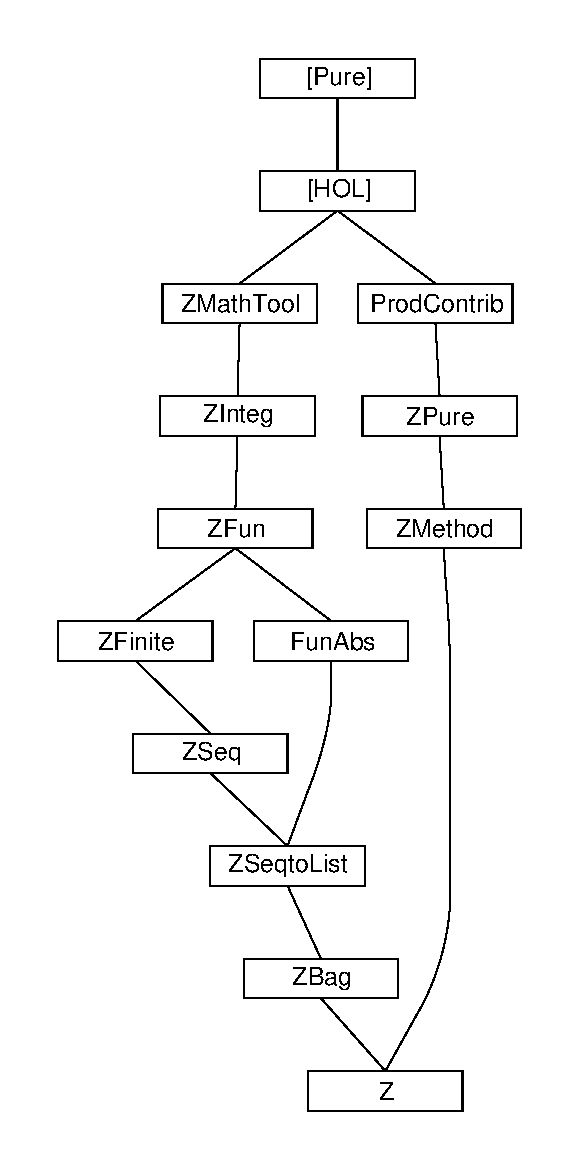
\includegraphics[width=\textwidth]{session_graph}
  \end{center}
  \caption{Session Graph\label{fig:session_graph}}
\end{figure}

%
\begin{isabellebody}%
\def\isabellecontext{ZMathTool}%
%
\isamarkupheader{Core of the Mathematical Toolkit%
}
\isamarkuptrue%
%
\isadelimtheory
%
\endisadelimtheory
%
\isatagtheory
\isacommand{theory}\isamarkupfalse%
\ ZMathTool\ \isakeyword{imports}\ \ Finite{\isacharunderscore}Set\ Sum{\isacharunderscore}Type\ Main\ \isakeyword{begin}%
\endisatagtheory
{\isafoldtheory}%
%
\isadelimtheory
%
\endisadelimtheory
\isanewline
\isanewline
\isacommand{types}\isamarkupfalse%
\ \ \ \ \ \ \ \ {\isacharparenleft}{\isacharprime}a{\isacharcomma}{\isacharprime}b{\isacharparenright}\ {\isachardoublequoteopen}{\isacharless}{\isacharequal}{\isachargreater}{\isachardoublequoteclose}\ {\isacharequal}\ {\isachardoublequoteopen}{\isacharparenleft}{\isacharprime}a{\isacharasterisk}{\isacharprime}b{\isacharparenright}\ set{\isachardoublequoteclose}\ \ \ \ \ {\isacharparenleft}\isakeyword{infixr}\ {\isadigit{2}}{\isadigit{0}}{\isacharparenright}\isanewline
\isanewline
\isacommand{consts}\isamarkupfalse%
\isanewline
\isanewline
idZ\ \ \ \ \ \ \ \ \ \ {\isacharcolon}{\isacharcolon}{\isachardoublequoteopen}{\isacharprime}a\ set\ {\isacharequal}{\isachargreater}\ {\isacharparenleft}{\isacharprime}a\ {\isacharless}{\isacharequal}{\isachargreater}\ {\isacharprime}a{\isacharparenright}{\isachardoublequoteclose}\isanewline
forw{\isacharunderscore}comp\ \ \ \ {\isacharcolon}{\isacharcolon}{\isachardoublequoteopen}{\isacharbrackleft}{\isacharprime}a\ {\isacharless}{\isacharequal}{\isachargreater}\ {\isacharprime}b{\isacharcomma}\ {\isacharprime}b\ {\isacharless}{\isacharequal}{\isachargreater}\ {\isacharprime}c{\isacharbrackright}\ {\isacharequal}{\isachargreater}\ {\isacharparenleft}{\isacharprime}a\ {\isacharless}{\isacharequal}{\isachargreater}\ {\isacharprime}c{\isacharparenright}{\isachardoublequoteclose}\ \ {\isacharparenleft}{\isachardoublequoteopen}{\isacharunderscore}\ {\isacharpercent}{\isacharsemicolon}\ {\isacharunderscore}{\isachardoublequoteclose}\ \ {\isacharbrackleft}{\isadigit{6}}{\isadigit{0}}{\isacharcomma}{\isadigit{6}}{\isadigit{1}}{\isacharbrackright}\ {\isadigit{6}}{\isadigit{0}}{\isacharparenright}\isanewline
dom{\isacharunderscore}restr\ \ \ \ {\isacharcolon}{\isacharcolon}{\isachardoublequoteopen}{\isacharbrackleft}{\isacharprime}a\ set\ {\isacharcomma}\ {\isacharprime}a\ {\isacharless}{\isacharequal}{\isachargreater}\ {\isacharprime}b{\isacharbrackright}\ {\isacharequal}{\isachargreater}\ {\isacharparenleft}{\isacharprime}a\ {\isacharless}{\isacharequal}{\isachargreater}\ {\isacharprime}b{\isacharparenright}{\isachardoublequoteclose}\ \ \ \ {\isacharparenleft}{\isachardoublequoteopen}{\isacharunderscore}\ {\isacharless}{\isacharcolon}\ {\isacharunderscore}{\isachardoublequoteclose}\ \ {\isacharbrackleft}{\isadigit{7}}{\isadigit{1}}{\isacharcomma}{\isadigit{7}}{\isadigit{0}}{\isacharbrackright}\ {\isadigit{7}}{\isadigit{0}}{\isacharparenright}\isanewline
ran{\isacharunderscore}restr\ \ \ \ {\isacharcolon}{\isacharcolon}{\isachardoublequoteopen}{\isacharbrackleft}{\isacharprime}a\ {\isacharless}{\isacharequal}{\isachargreater}\ {\isacharprime}b{\isacharcomma}\ {\isacharparenleft}{\isacharprime}b{\isacharparenright}set{\isacharbrackright}\ {\isacharequal}{\isachargreater}\ {\isacharprime}a\ {\isacharless}{\isacharequal}{\isachargreater}\ {\isacharprime}b{\isachardoublequoteclose}\ \ \ \ \ \ {\isacharparenleft}{\isachardoublequoteopen}{\isacharunderscore}\ {\isacharcolon}{\isachargreater}\ {\isacharunderscore}{\isachardoublequoteclose}\ \ {\isacharbrackleft}{\isadigit{6}}{\isadigit{5}}{\isacharcomma}{\isadigit{6}}{\isadigit{6}}{\isacharbrackright}\ {\isadigit{6}}{\isadigit{5}}{\isacharparenright}\isanewline
dom{\isacharunderscore}substr\ \ \ {\isacharcolon}{\isacharcolon}{\isachardoublequoteopen}{\isacharbrackleft}\ {\isacharparenleft}{\isacharprime}a{\isacharparenright}set\ {\isacharcomma}\ {\isacharprime}a\ {\isacharless}{\isacharequal}{\isachargreater}\ {\isacharprime}b{\isacharbrackright}\ {\isacharequal}{\isachargreater}\ {\isacharprime}a\ {\isacharless}{\isacharequal}{\isachargreater}\ {\isacharprime}b{\isachardoublequoteclose}\ \ \ \ {\isacharparenleft}{\isachardoublequoteopen}{\isacharunderscore}\ {\isacharless}{\isacharminus}{\isacharcolon}\ {\isacharunderscore}{\isachardoublequoteclose}\ {\isacharbrackleft}{\isadigit{7}}{\isadigit{1}}{\isacharcomma}{\isadigit{7}}{\isadigit{0}}{\isacharbrackright}\ {\isadigit{7}}{\isadigit{0}}{\isacharparenright}\isanewline
ran{\isacharunderscore}substr\ \ \ {\isacharcolon}{\isacharcolon}{\isachardoublequoteopen}{\isacharbrackleft}{\isacharprime}a\ {\isacharless}{\isacharequal}{\isachargreater}\ {\isacharprime}b{\isacharcomma}\ {\isacharparenleft}{\isacharprime}b{\isacharparenright}\ set{\isacharbrackright}\ {\isacharequal}{\isachargreater}\ {\isacharparenleft}{\isacharprime}a\ {\isacharless}{\isacharequal}{\isachargreater}\ {\isacharprime}b{\isacharparenright}{\isachardoublequoteclose}\ \ \ {\isacharparenleft}{\isachardoublequoteopen}{\isacharunderscore}\ {\isacharcolon}{\isacharminus}{\isachargreater}\ {\isacharunderscore}{\isachardoublequoteclose}\ {\isacharbrackleft}{\isadigit{6}}{\isadigit{5}}{\isacharcomma}{\isadigit{6}}{\isadigit{6}}{\isacharbrackright}\ {\isadigit{6}}{\isadigit{5}}{\isacharparenright}\isanewline
\isanewline
trans{\isacharunderscore}clos\ \ \ {\isacharcolon}{\isacharcolon}{\isachardoublequoteopen}{\isacharparenleft}{\isacharprime}a\ {\isacharless}{\isacharequal}{\isachargreater}\ {\isacharprime}a{\isacharparenright}\ {\isacharequal}{\isachargreater}\ {\isacharparenleft}{\isacharprime}a\ {\isacharless}{\isacharequal}{\isachargreater}\ {\isacharprime}a{\isacharparenright}\ {\isachardoublequoteclose}\ \ \ \ \ \ \ \ \ \ \ \ {\isacharparenleft}{\isachardoublequoteopen}{\isacharunderscore}\ {\isacharpercent}{\isacharplus}{\isachardoublequoteclose}\ \ \ \ \ {\isacharbrackleft}{\isadigit{1}}{\isadigit{0}}{\isadigit{0}}{\isadigit{0}}{\isacharbrackright}\ {\isadigit{9}}{\isadigit{9}}{\isadigit{9}}{\isacharparenright}\isanewline
ref{\isacharunderscore}trans{\isacharunderscore}clos{\isacharcolon}{\isacharcolon}{\isachardoublequoteopen}{\isacharparenleft}{\isacharprime}a\ {\isacharless}{\isacharequal}{\isachargreater}\ {\isacharprime}a{\isacharparenright}\ {\isacharequal}{\isachargreater}\ {\isacharparenleft}{\isacharprime}a\ {\isacharless}{\isacharequal}{\isachargreater}\ {\isacharprime}a{\isacharparenright}\ {\isachardoublequoteclose}\ \ \ \ \ \ \ \ \ \ \ {\isacharparenleft}{\isachardoublequoteopen}{\isacharunderscore}\ {\isacharpercent}{\isacharasterisk}{\isachardoublequoteclose}\ \ \ \ \ {\isacharbrackleft}{\isadigit{1}}{\isadigit{0}}{\isadigit{0}}{\isadigit{0}}{\isacharbrackright}\ {\isadigit{9}}{\isadigit{9}}{\isadigit{9}}{\isacharparenright}\isanewline
\isanewline
partial{\isacharunderscore}func\ {\isacharcolon}{\isacharcolon}{\isachardoublequoteopen}{\isacharbrackleft}{\isacharprime}a\ set{\isacharcomma}{\isacharprime}b\ set{\isacharbrackright}\ {\isacharequal}{\isachargreater}\ {\isacharparenleft}{\isacharprime}a\ {\isacharless}{\isacharequal}{\isachargreater}\ {\isacharprime}b{\isacharparenright}\ set{\isachardoublequoteclose}\ \ \ \ \ {\isacharparenleft}{\isachardoublequoteopen}{\isacharunderscore}\ {\isacharminus}{\isacharbar}{\isacharminus}{\isachargreater}\ {\isacharunderscore}{\isachardoublequoteclose}\ \ \ {\isacharbrackleft}{\isadigit{5}}{\isadigit{4}}{\isacharcomma}{\isadigit{5}}{\isadigit{3}}{\isacharbrackright}\ {\isadigit{5}}{\isadigit{3}}{\isacharparenright}\isanewline
\isanewline
total{\isacharunderscore}func\ \ \ {\isacharcolon}{\isacharcolon}{\isachardoublequoteopen}{\isacharbrackleft}{\isacharprime}a\ set{\isacharcomma}{\isacharprime}b\ set{\isacharbrackright}\ {\isacharequal}{\isachargreater}\ {\isacharparenleft}{\isacharprime}a\ {\isacharless}{\isacharequal}{\isachargreater}\ {\isacharprime}b{\isacharparenright}\ set{\isachardoublequoteclose}\ \ \ \ \ {\isacharparenleft}{\isachardoublequoteopen}{\isacharunderscore}\ {\isacharminus}{\isacharminus}{\isacharminus}{\isachargreater}\ {\isacharunderscore}{\isachardoublequoteclose}\ \ \ {\isacharbrackleft}{\isadigit{5}}{\isadigit{4}}{\isacharcomma}{\isadigit{5}}{\isadigit{3}}{\isacharbrackright}\ {\isadigit{5}}{\isadigit{3}}{\isacharparenright}\isanewline
\isanewline
partial{\isacharunderscore}inj\ \ {\isacharcolon}{\isacharcolon}{\isachardoublequoteopen}{\isacharbrackleft}{\isacharprime}a\ set{\isacharcomma}{\isacharprime}b\ set{\isacharbrackright}\ {\isacharequal}{\isachargreater}\ {\isacharparenleft}{\isacharprime}a\ {\isacharless}{\isacharequal}{\isachargreater}\ {\isacharprime}b{\isacharparenright}\ set{\isachardoublequoteclose}\ \ \ \ \ {\isacharparenleft}{\isachardoublequoteopen}{\isacharunderscore}\ {\isachargreater}{\isacharminus}{\isacharbar}{\isacharminus}{\isachargreater}\ {\isacharunderscore}{\isachardoublequoteclose}\ \ {\isacharbrackleft}{\isadigit{5}}{\isadigit{4}}{\isacharcomma}{\isadigit{5}}{\isadigit{3}}{\isacharbrackright}\ {\isadigit{5}}{\isadigit{3}}{\isacharparenright}\isanewline
\isanewline
total{\isacharunderscore}inj\ \ \ \ {\isacharcolon}{\isacharcolon}{\isachardoublequoteopen}{\isacharbrackleft}{\isacharprime}a\ set{\isacharcomma}{\isacharprime}b\ set{\isacharbrackright}\ {\isacharequal}{\isachargreater}\ {\isacharparenleft}{\isacharprime}a\ {\isacharless}{\isacharequal}{\isachargreater}\ {\isacharprime}b{\isacharparenright}\ set{\isachardoublequoteclose}\ \ \ \ \ {\isacharparenleft}{\isachardoublequoteopen}{\isacharunderscore}\ {\isachargreater}{\isacharminus}{\isacharminus}{\isachargreater}\ {\isacharunderscore}{\isachardoublequoteclose}\ \ \ {\isacharbrackleft}{\isadigit{5}}{\isadigit{4}}{\isacharcomma}{\isadigit{5}}{\isadigit{3}}{\isacharbrackright}\ {\isadigit{5}}{\isadigit{3}}{\isacharparenright}\isanewline
\isanewline
partial{\isacharunderscore}surj\ {\isacharcolon}{\isacharcolon}{\isachardoublequoteopen}{\isacharbrackleft}{\isacharprime}a\ set{\isacharcomma}{\isacharprime}b\ set{\isacharbrackright}\ {\isacharequal}{\isachargreater}\ {\isacharparenleft}{\isacharprime}a\ {\isacharless}{\isacharequal}{\isachargreater}\ {\isacharprime}b{\isacharparenright}\ set{\isachardoublequoteclose}\ \ \ \ \ {\isacharparenleft}{\isachardoublequoteopen}{\isacharunderscore}\ {\isacharminus}{\isacharbar}{\isacharminus}{\isachargreater}{\isachargreater}\ {\isacharunderscore}{\isachardoublequoteclose}\ \ {\isacharbrackleft}{\isadigit{5}}{\isadigit{4}}{\isacharcomma}{\isadigit{5}}{\isadigit{3}}{\isacharbrackright}\ {\isadigit{5}}{\isadigit{3}}{\isacharparenright}\isanewline
\isanewline
total{\isacharunderscore}surj\ \ \ {\isacharcolon}{\isacharcolon}{\isachardoublequoteopen}{\isacharbrackleft}{\isacharprime}a\ set{\isacharcomma}{\isacharprime}b\ set{\isacharbrackright}\ {\isacharequal}{\isachargreater}\ {\isacharparenleft}{\isacharprime}a\ {\isacharless}{\isacharequal}{\isachargreater}\ {\isacharprime}b{\isacharparenright}\ set{\isachardoublequoteclose}\ \ \ \ \ {\isacharparenleft}{\isachardoublequoteopen}{\isacharunderscore}\ {\isacharminus}{\isacharminus}{\isachargreater}{\isachargreater}\ {\isacharunderscore}{\isachardoublequoteclose}\ \ \ {\isacharbrackleft}{\isadigit{5}}{\isadigit{4}}{\isacharcomma}{\isadigit{5}}{\isadigit{3}}{\isacharbrackright}\ {\isadigit{5}}{\isadigit{3}}{\isacharparenright}\isanewline
\isanewline
biject\ \ \ \ \ \ \ {\isacharcolon}{\isacharcolon}{\isachardoublequoteopen}{\isacharbrackleft}{\isacharprime}a\ set{\isacharcomma}{\isacharprime}b\ set{\isacharbrackright}\ {\isacharequal}{\isachargreater}\ {\isacharparenleft}{\isacharprime}a\ {\isacharless}{\isacharequal}{\isachargreater}\ {\isacharprime}b{\isacharparenright}\ set{\isachardoublequoteclose}\ \ \ \ \ {\isacharparenleft}{\isachardoublequoteopen}{\isacharunderscore}\ {\isachargreater}{\isacharminus}{\isacharminus}{\isachargreater}{\isachargreater}\ {\isacharunderscore}{\isachardoublequoteclose}\ \ {\isacharbrackleft}{\isadigit{5}}{\isadigit{4}}{\isacharcomma}{\isadigit{5}}{\isadigit{3}}{\isacharbrackright}\ {\isadigit{5}}{\isadigit{3}}{\isacharparenright}\isanewline
\isanewline
fin{\isacharunderscore}part{\isacharunderscore}func{\isacharcolon}{\isacharcolon}{\isachardoublequoteopen}{\isacharbrackleft}{\isacharprime}a\ set{\isacharcomma}{\isacharprime}b\ set{\isacharbrackright}\ {\isacharequal}{\isachargreater}\ {\isacharparenleft}{\isacharprime}a\ {\isacharless}{\isacharequal}{\isachargreater}\ {\isacharprime}b{\isacharparenright}\ set{\isachardoublequoteclose}\ \ \ \ \ {\isacharparenleft}{\isachardoublequoteopen}{\isacharunderscore}\ {\isacharminus}{\isacharbar}{\isacharbar}{\isacharminus}{\isachargreater}\ {\isacharunderscore}{\isachardoublequoteclose}\ \ {\isacharbrackleft}{\isadigit{5}}{\isadigit{4}}{\isacharcomma}{\isadigit{5}}{\isadigit{3}}{\isacharbrackright}\ {\isadigit{5}}{\isadigit{3}}{\isacharparenright}\isanewline
\isanewline
fin{\isacharunderscore}part{\isacharunderscore}inj\ {\isacharcolon}{\isacharcolon}{\isachardoublequoteopen}{\isacharbrackleft}{\isacharprime}a\ set{\isacharcomma}{\isacharprime}b\ set{\isacharbrackright}\ {\isacharequal}{\isachargreater}\ {\isacharparenleft}{\isacharprime}a\ {\isacharless}{\isacharequal}{\isachargreater}\ {\isacharprime}b{\isacharparenright}\ set{\isachardoublequoteclose}\ \ \ \ \ {\isacharparenleft}{\isachardoublequoteopen}{\isacharunderscore}\ {\isachargreater}{\isacharminus}{\isacharbar}{\isacharbar}{\isacharminus}{\isachargreater}\ {\isacharunderscore}{\isachardoublequoteclose}\ {\isacharbrackleft}{\isadigit{5}}{\isadigit{4}}{\isacharcomma}{\isadigit{5}}{\isadigit{3}}{\isacharbrackright}\ {\isadigit{5}}{\isadigit{3}}{\isacharparenright}\isanewline
\isanewline
rel\ \ \ \ \ \ \ \ \ \ {\isacharcolon}{\isacharcolon}{\isachardoublequoteopen}{\isacharbrackleft}{\isacharprime}a\ set{\isacharcomma}\ {\isacharprime}b\ set{\isacharbrackright}\ {\isacharequal}{\isachargreater}\ {\isacharparenleft}{\isacharprime}a\ {\isacharless}{\isacharequal}{\isachargreater}\ {\isacharprime}b{\isacharparenright}\ set{\isachardoublequoteclose}\ \ \ \ {\isacharparenleft}{\isachardoublequoteopen}{\isacharunderscore}\ {\isacharless}{\isacharminus}{\isacharminus}{\isachargreater}\ {\isacharunderscore}{\isachardoublequoteclose}\ \ \ {\isacharbrackleft}{\isadigit{5}}{\isadigit{4}}{\isacharcomma}{\isadigit{5}}{\isadigit{3}}{\isacharbrackright}\ {\isadigit{5}}{\isadigit{3}}{\isacharparenright}\isanewline
rel{\isacharunderscore}appl\ \ \ \ \ {\isacharcolon}{\isacharcolon}{\isachardoublequoteopen}{\isacharbrackleft}{\isacharprime}a{\isacharless}{\isacharequal}{\isachargreater}{\isacharprime}b{\isacharcomma}{\isacharprime}a{\isacharbrackright}\ {\isacharequal}{\isachargreater}\ {\isacharprime}b{\isachardoublequoteclose}\ \ \ \ \ \ \ \ \ \ \ \ \ \ \ \ \ \ \ \ \ {\isacharparenleft}{\isachardoublequoteopen}{\isacharunderscore}\ {\isacharpercent}{\isacharcircum}\ {\isacharunderscore}{\isachardoublequoteclose}\ \ \ \ \ {\isacharbrackleft}{\isadigit{9}}{\isadigit{0}}{\isacharcomma}{\isadigit{9}}{\isadigit{1}}{\isacharbrackright}\ {\isadigit{9}}{\isadigit{0}}{\isacharparenright}\isanewline
override\ \ \ \ \ {\isacharcolon}{\isacharcolon}{\isachardoublequoteopen}{\isacharbrackleft}{\isacharprime}a\ {\isacharless}{\isacharequal}{\isachargreater}\ {\isacharprime}b{\isacharcomma}\ {\isacharprime}a\ {\isacharless}{\isacharequal}{\isachargreater}\ {\isacharprime}b{\isacharbrackright}\ {\isacharequal}{\isachargreater}\ {\isacharparenleft}{\isacharprime}a\ {\isacharless}{\isacharequal}{\isachargreater}\ {\isacharprime}b{\isacharparenright}{\isachardoublequoteclose}\ \ {\isacharparenleft}{\isachardoublequoteopen}{\isacharunderscore}\ {\isacharprime}{\isacharparenleft}{\isacharplus}{\isacharprime}{\isacharparenright}\ {\isacharunderscore}{\isachardoublequoteclose}\ \ {\isacharbrackleft}{\isadigit{5}}{\isadigit{5}}{\isacharcomma}{\isadigit{5}}{\isadigit{6}}{\isacharbrackright}\ {\isadigit{5}}{\isadigit{5}}{\isacharparenright}\isanewline
iter\ \ \ \ \ \ \ \ \ {\isacharcolon}{\isacharcolon}{\isachardoublequoteopen}{\isacharbrackleft}{\isacharprime}a\ {\isacharless}{\isacharequal}{\isachargreater}\ {\isacharprime}a{\isacharcomma}\ int{\isacharbrackright}\ {\isacharequal}{\isachargreater}\ {\isacharparenleft}{\isacharprime}a\ {\isacharless}{\isacharequal}{\isachargreater}\ {\isacharprime}a{\isacharparenright}\ {\isachardoublequoteclose}\isanewline
numb{\isacharunderscore}range\ \ \ {\isacharcolon}{\isacharcolon}{\isachardoublequoteopen}{\isacharbrackleft}int{\isacharcomma}int{\isacharbrackright}\ {\isacharequal}{\isachargreater}\ {\isacharparenleft}int{\isacharparenright}\ set{\isachardoublequoteclose}\ \ \ \ \ \ \ \ \ \ \ \ \ \ \ \ \ {\isacharparenleft}{\isachardoublequoteopen}\ {\isacharunderscore}\ {\isachardot}{\isachardot}\ {\isacharunderscore}{\isachardoublequoteclose}\ \ \ \ {\isacharbrackleft}{\isadigit{5}}{\isadigit{0}}{\isacharcomma}{\isadigit{5}}{\isadigit{1}}{\isacharbrackright}\ {\isadigit{5}}{\isadigit{0}}{\isacharparenright}\isanewline
\isanewline
\isanewline
\isacommand{syntax}\isamarkupfalse%
\ {\isacharparenleft}xsymbols{\isacharparenright}\isanewline
idZ\ \ \ \ \ \ \ \ \ \ {\isacharcolon}{\isacharcolon}{\isachardoublequoteopen}{\isacharprime}a\ set\ {\isacharequal}{\isachargreater}\ {\isacharparenleft}{\isacharprime}a\ {\isacharless}{\isacharequal}{\isachargreater}\ {\isacharprime}a{\isacharparenright}{\isachardoublequoteclose}\ \ \ \ \ \ \ \ \ \ \ \ \ \ \ \ \ \ {\isacharparenleft}{\isachardoublequoteopen}{\isasymid}{\isachardoublequoteclose}{\isacharparenright}\isanewline
forw{\isacharunderscore}comp\ \ \ \ {\isacharcolon}{\isacharcolon}{\isachardoublequoteopen}{\isacharbrackleft}{\isacharprime}a\ {\isacharless}{\isacharequal}{\isachargreater}\ {\isacharprime}b{\isacharcomma}\ {\isacharprime}b\ {\isacharless}{\isacharequal}{\isachargreater}\ {\isacharprime}c{\isacharbrackright}\ {\isacharequal}{\isachargreater}\ {\isacharparenleft}{\isacharprime}a\ {\isacharless}{\isacharequal}{\isachargreater}\ {\isacharprime}c{\isacharparenright}{\isachardoublequoteclose}\ \ {\isacharparenleft}{\isachardoublequoteopen}{\isacharunderscore}\ {\isasymcomp}\ {\isacharunderscore}{\isachardoublequoteclose}\ \ {\isacharbrackleft}{\isadigit{6}}{\isadigit{0}}{\isacharcomma}{\isadigit{6}}{\isadigit{1}}{\isacharbrackright}\ {\isadigit{6}}{\isadigit{0}}{\isacharparenright}\isanewline
dom{\isacharunderscore}restr\ \ \ \ {\isacharcolon}{\isacharcolon}{\isachardoublequoteopen}{\isacharbrackleft}{\isacharprime}a\ set\ {\isacharcomma}\ {\isacharprime}a\ {\isacharless}{\isacharequal}{\isachargreater}\ {\isacharprime}b{\isacharbrackright}\ {\isacharequal}{\isachargreater}\ {\isacharparenleft}{\isacharprime}a\ {\isacharless}{\isacharequal}{\isachargreater}\ {\isacharprime}b{\isacharparenright}{\isachardoublequoteclose}\ \ \ \ {\isacharparenleft}{\isachardoublequoteopen}{\isacharunderscore}\ {\isasymdres}\ {\isacharunderscore}{\isachardoublequoteclose}\ \ {\isacharbrackleft}{\isadigit{7}}{\isadigit{1}}{\isacharcomma}{\isadigit{7}}{\isadigit{0}}{\isacharbrackright}\ {\isadigit{7}}{\isadigit{0}}{\isacharparenright}\isanewline
ran{\isacharunderscore}restr\ \ \ \ {\isacharcolon}{\isacharcolon}{\isachardoublequoteopen}{\isacharbrackleft}{\isacharprime}a\ {\isacharless}{\isacharequal}{\isachargreater}\ {\isacharprime}b{\isacharcomma}\ {\isacharparenleft}{\isacharprime}b{\isacharparenright}set{\isacharbrackright}\ {\isacharequal}{\isachargreater}\ {\isacharprime}a\ {\isacharless}{\isacharequal}{\isachargreater}\ {\isacharprime}b{\isachardoublequoteclose}\ \ \ \ \ \ {\isacharparenleft}{\isachardoublequoteopen}{\isacharunderscore}\ {\isasymrres}\ {\isacharunderscore}{\isachardoublequoteclose}\ \ {\isacharbrackleft}{\isadigit{6}}{\isadigit{5}}{\isacharcomma}{\isadigit{6}}{\isadigit{6}}{\isacharbrackright}\ {\isadigit{6}}{\isadigit{5}}{\isacharparenright}\isanewline
dom{\isacharunderscore}substr\ \ \ {\isacharcolon}{\isacharcolon}{\isachardoublequoteopen}{\isacharbrackleft}\ {\isacharparenleft}{\isacharprime}a{\isacharparenright}set\ {\isacharcomma}\ {\isacharprime}a\ {\isacharless}{\isacharequal}{\isachargreater}\ {\isacharprime}b{\isacharbrackright}\ {\isacharequal}{\isachargreater}\ {\isacharprime}a\ {\isacharless}{\isacharequal}{\isachargreater}\ {\isacharprime}b{\isachardoublequoteclose}\ \ \ \ {\isacharparenleft}{\isachardoublequoteopen}{\isacharunderscore}\ {\isasymndres}\ {\isacharunderscore}{\isachardoublequoteclose}\ {\isacharbrackleft}{\isadigit{7}}{\isadigit{1}}{\isacharcomma}{\isadigit{7}}{\isadigit{0}}{\isacharbrackright}\ {\isadigit{7}}{\isadigit{0}}{\isacharparenright}\isanewline
ran{\isacharunderscore}substr\ \ \ {\isacharcolon}{\isacharcolon}{\isachardoublequoteopen}{\isacharbrackleft}{\isacharprime}a\ {\isacharless}{\isacharequal}{\isachargreater}\ {\isacharprime}b{\isacharcomma}\ {\isacharparenleft}{\isacharprime}b{\isacharparenright}\ set{\isacharbrackright}\ {\isacharequal}{\isachargreater}\ {\isacharparenleft}{\isacharprime}a\ {\isacharless}{\isacharequal}{\isachargreater}\ {\isacharprime}b{\isacharparenright}{\isachardoublequoteclose}\ \ \ {\isacharparenleft}{\isachardoublequoteopen}{\isacharunderscore}\ {\isasymnrres}\ {\isacharunderscore}{\isachardoublequoteclose}\ {\isacharbrackleft}{\isadigit{6}}{\isadigit{5}}{\isacharcomma}{\isadigit{6}}{\isadigit{6}}{\isacharbrackright}\ {\isadigit{6}}{\isadigit{5}}{\isacharparenright}\isanewline
\isanewline
trans{\isacharunderscore}clos\ \ \ {\isacharcolon}{\isacharcolon}{\isachardoublequoteopen}{\isacharparenleft}{\isacharprime}a\ {\isacharless}{\isacharequal}{\isachargreater}\ {\isacharprime}a{\isacharparenright}\ {\isacharequal}{\isachargreater}\ {\isacharparenleft}{\isacharprime}a\ {\isacharless}{\isacharequal}{\isachargreater}\ {\isacharprime}a{\isacharparenright}\ {\isachardoublequoteclose}\ \ \ \ \ \ \ \ \ \ \ \ {\isacharparenleft}{\isachardoublequoteopen}{\isacharunderscore}\ {\isasymplus}\ {\isachardoublequoteclose}\ \ \ {\isacharbrackleft}{\isadigit{1}}{\isadigit{0}}{\isadigit{0}}{\isadigit{0}}{\isacharbrackright}\ {\isadigit{9}}{\isadigit{9}}{\isadigit{9}}{\isacharparenright}\isanewline
ref{\isacharunderscore}trans{\isacharunderscore}clos{\isacharcolon}{\isacharcolon}{\isachardoublequoteopen}{\isacharparenleft}{\isacharprime}a\ {\isacharless}{\isacharequal}{\isachargreater}\ {\isacharprime}a{\isacharparenright}\ {\isacharequal}{\isachargreater}\ {\isacharparenleft}{\isacharprime}a\ {\isacharless}{\isacharequal}{\isachargreater}\ {\isacharprime}a{\isacharparenright}\ {\isachardoublequoteclose}\ \ \ \ \ \ \ \ \ \ \ {\isacharparenleft}{\isachardoublequoteopen}{\isacharunderscore}\ {\isasymstar}{\isachardoublequoteclose}\ \ \ \ {\isacharbrackleft}{\isadigit{1}}{\isadigit{0}}{\isadigit{0}}{\isadigit{0}}{\isacharbrackright}\ {\isadigit{9}}{\isadigit{9}}{\isadigit{9}}{\isacharparenright}\isanewline
\isanewline
partial{\isacharunderscore}func\ {\isacharcolon}{\isacharcolon}{\isachardoublequoteopen}{\isacharbrackleft}{\isacharprime}a\ set{\isacharcomma}{\isacharprime}b\ set{\isacharbrackright}\ {\isacharequal}{\isachargreater}\ {\isacharparenleft}{\isacharprime}a\ {\isacharless}{\isacharequal}{\isachargreater}\ {\isacharprime}b{\isacharparenright}\ set{\isachardoublequoteclose}\ \ \ \ \ {\isacharparenleft}{\isachardoublequoteopen}{\isacharunderscore}\ {\isasympfun}\ {\isacharunderscore}{\isachardoublequoteclose}\ \ {\isacharbrackleft}{\isadigit{5}}{\isadigit{4}}{\isacharcomma}{\isadigit{5}}{\isadigit{3}}{\isacharbrackright}\ {\isadigit{5}}{\isadigit{3}}{\isacharparenright}\isanewline
total{\isacharunderscore}func\ \ \ {\isacharcolon}{\isacharcolon}{\isachardoublequoteopen}{\isacharbrackleft}{\isacharprime}a\ set{\isacharcomma}{\isacharprime}b\ set{\isacharbrackright}\ {\isacharequal}{\isachargreater}\ {\isacharparenleft}{\isacharprime}a\ {\isacharless}{\isacharequal}{\isachargreater}\ {\isacharprime}b{\isacharparenright}\ set{\isachardoublequoteclose}\ \ \ \ \ {\isacharparenleft}{\isachardoublequoteopen}{\isacharunderscore}\ {\isasymfun}\ {\isacharunderscore}{\isachardoublequoteclose}\ \ \ {\isacharbrackleft}{\isadigit{5}}{\isadigit{4}}{\isacharcomma}{\isadigit{5}}{\isadigit{3}}{\isacharbrackright}\ {\isadigit{5}}{\isadigit{3}}{\isacharparenright}\isanewline
partial{\isacharunderscore}inj\ \ {\isacharcolon}{\isacharcolon}{\isachardoublequoteopen}{\isacharbrackleft}{\isacharprime}a\ set{\isacharcomma}{\isacharprime}b\ set{\isacharbrackright}\ {\isacharequal}{\isachargreater}\ {\isacharparenleft}{\isacharprime}a\ {\isacharless}{\isacharequal}{\isachargreater}\ {\isacharprime}b{\isacharparenright}\ set{\isachardoublequoteclose}\ \ \ \ \ {\isacharparenleft}{\isachardoublequoteopen}{\isacharunderscore}\ {\isasympinj}\ {\isacharunderscore}{\isachardoublequoteclose}\ \ {\isacharbrackleft}{\isadigit{5}}{\isadigit{4}}{\isacharcomma}{\isadigit{5}}{\isadigit{3}}{\isacharbrackright}\ {\isadigit{5}}{\isadigit{3}}{\isacharparenright}\isanewline
total{\isacharunderscore}inj\ \ \ \ {\isacharcolon}{\isacharcolon}{\isachardoublequoteopen}{\isacharbrackleft}{\isacharprime}a\ set{\isacharcomma}{\isacharprime}b\ set{\isacharbrackright}\ {\isacharequal}{\isachargreater}\ {\isacharparenleft}{\isacharprime}a\ {\isacharless}{\isacharequal}{\isachargreater}\ {\isacharprime}b{\isacharparenright}\ set{\isachardoublequoteclose}\ \ \ \ \ {\isacharparenleft}{\isachardoublequoteopen}{\isacharunderscore}\ {\isasyminj}\ {\isacharunderscore}{\isachardoublequoteclose}\ \ \ {\isacharbrackleft}{\isadigit{5}}{\isadigit{4}}{\isacharcomma}{\isadigit{5}}{\isadigit{3}}{\isacharbrackright}\ {\isadigit{5}}{\isadigit{3}}{\isacharparenright}\isanewline
partial{\isacharunderscore}surj\ {\isacharcolon}{\isacharcolon}{\isachardoublequoteopen}{\isacharbrackleft}{\isacharprime}a\ set{\isacharcomma}{\isacharprime}b\ set{\isacharbrackright}\ {\isacharequal}{\isachargreater}\ {\isacharparenleft}{\isacharprime}a\ {\isacharless}{\isacharequal}{\isachargreater}\ {\isacharprime}b{\isacharparenright}\ set{\isachardoublequoteclose}\ \ \ \ \ {\isacharparenleft}{\isachardoublequoteopen}{\isacharunderscore}\ {\isasympsurj}\ {\isacharunderscore}{\isachardoublequoteclose}\ {\isacharbrackleft}{\isadigit{5}}{\isadigit{4}}{\isacharcomma}{\isadigit{5}}{\isadigit{3}}{\isacharbrackright}\ {\isadigit{5}}{\isadigit{3}}{\isacharparenright}\isanewline
total{\isacharunderscore}surj\ \ \ {\isacharcolon}{\isacharcolon}{\isachardoublequoteopen}{\isacharbrackleft}{\isacharprime}a\ set{\isacharcomma}{\isacharprime}b\ set{\isacharbrackright}\ {\isacharequal}{\isachargreater}\ {\isacharparenleft}{\isacharprime}a\ {\isacharless}{\isacharequal}{\isachargreater}\ {\isacharprime}b{\isacharparenright}\ set{\isachardoublequoteclose}\ \ \ \ \ {\isacharparenleft}{\isachardoublequoteopen}{\isacharunderscore}\ {\isasymsurj}\ {\isacharunderscore}{\isachardoublequoteclose}\ \ {\isacharbrackleft}{\isadigit{5}}{\isadigit{4}}{\isacharcomma}{\isadigit{5}}{\isadigit{3}}{\isacharbrackright}\ {\isadigit{5}}{\isadigit{3}}{\isacharparenright}\isanewline
biject\ \ \ \ \ \ \ {\isacharcolon}{\isacharcolon}{\isachardoublequoteopen}{\isacharbrackleft}{\isacharprime}a\ set{\isacharcomma}{\isacharprime}b\ set{\isacharbrackright}\ {\isacharequal}{\isachargreater}\ {\isacharparenleft}{\isacharprime}a\ {\isacharless}{\isacharequal}{\isachargreater}\ {\isacharprime}b{\isacharparenright}\ set{\isachardoublequoteclose}\ \ \ \ \ {\isacharparenleft}{\isachardoublequoteopen}{\isacharunderscore}\ {\isasymbij}\ {\isacharunderscore}{\isachardoublequoteclose}\ \ \ {\isacharbrackleft}{\isadigit{5}}{\isadigit{4}}{\isacharcomma}{\isadigit{5}}{\isadigit{3}}{\isacharbrackright}\ {\isadigit{5}}{\isadigit{3}}{\isacharparenright}\isanewline
override{\isacharcolon}{\isacharcolon}{\isachardoublequoteopen}{\isacharbrackleft}{\isacharprime}a\ {\isacharless}{\isacharequal}{\isachargreater}\ {\isacharprime}b{\isacharcomma}\ {\isacharprime}a\ {\isacharless}{\isacharequal}{\isachargreater}\ {\isacharprime}b{\isacharbrackright}\ {\isacharequal}{\isachargreater}\ {\isacharparenleft}{\isacharprime}a\ {\isacharless}{\isacharequal}{\isachargreater}\ {\isacharprime}b{\isacharparenright}{\isachardoublequoteclose}\ \ {\isacharparenleft}{\isachardoublequoteopen}{\isacharunderscore}\ {\isasymoplus}\ {\isacharunderscore}{\isachardoublequoteclose}\ {\isacharbrackleft}{\isadigit{5}}{\isadigit{5}}{\isacharcomma}{\isadigit{5}}{\isadigit{6}}{\isacharbrackright}\ {\isadigit{5}}{\isadigit{5}}{\isacharparenright}\isanewline
numb{\isacharunderscore}range\ \ \ {\isacharcolon}{\isacharcolon}{\isachardoublequoteopen}{\isacharbrackleft}int{\isacharcomma}int{\isacharbrackright}\ {\isacharequal}{\isachargreater}\ {\isacharparenleft}int{\isacharparenright}\ set{\isachardoublequoteclose}\ \ \ \ \ \ \ \ \ \ \ \ \ \ \ \ \ {\isacharparenleft}{\isachardoublequoteopen}{\isacharunderscore}\ {\isasymupto}\ {\isacharunderscore}{\isachardoublequoteclose}\ \ {\isacharbrackleft}{\isadigit{5}}{\isadigit{0}}{\isacharcomma}{\isadigit{5}}{\isadigit{1}}{\isacharbrackright}\ {\isadigit{5}}{\isadigit{0}}{\isacharparenright}\isanewline
fin{\isacharunderscore}part{\isacharunderscore}func{\isacharcolon}{\isacharcolon}{\isachardoublequoteopen}{\isacharbrackleft}{\isacharprime}a\ set{\isacharcomma}{\isacharprime}b\ set{\isacharbrackright}\ {\isacharequal}{\isachargreater}\ {\isacharparenleft}{\isacharprime}a\ {\isacharless}{\isacharequal}{\isachargreater}\ {\isacharprime}b{\isacharparenright}\ set{\isachardoublequoteclose}\ \ \ \ \ {\isacharparenleft}{\isachardoublequoteopen}{\isacharunderscore}\ {\isasymffun}\ {\isacharunderscore}{\isachardoublequoteclose}\ \ {\isacharbrackleft}{\isadigit{5}}{\isadigit{4}}{\isacharcomma}{\isadigit{5}}{\isadigit{3}}{\isacharbrackright}\ {\isadigit{5}}{\isadigit{3}}{\isacharparenright}\isanewline
fin{\isacharunderscore}part{\isacharunderscore}inj\ {\isacharcolon}{\isacharcolon}{\isachardoublequoteopen}{\isacharbrackleft}{\isacharprime}a\ set{\isacharcomma}{\isacharprime}b\ set{\isacharbrackright}\ {\isacharequal}{\isachargreater}\ {\isacharparenleft}{\isacharprime}a\ {\isacharless}{\isacharequal}{\isachargreater}\ {\isacharprime}b{\isacharparenright}\ set{\isachardoublequoteclose}\ \ \ \ \ {\isacharparenleft}{\isachardoublequoteopen}{\isacharunderscore}\ {\isasymfinj}\ {\isacharunderscore}{\isachardoublequoteclose}\ \ {\isacharbrackleft}{\isadigit{5}}{\isadigit{4}}{\isacharcomma}{\isadigit{5}}{\isadigit{3}}{\isacharbrackright}\ {\isadigit{5}}{\isadigit{3}}{\isacharparenright}\isanewline
rel\ \ \ \ \ \ \ \ \ \ {\isacharcolon}{\isacharcolon}{\isachardoublequoteopen}{\isacharbrackleft}{\isacharprime}a\ set{\isacharcomma}\ {\isacharprime}b\ set{\isacharbrackright}\ {\isacharequal}{\isachargreater}\ {\isacharparenleft}{\isacharprime}a\ {\isacharless}{\isacharequal}{\isachargreater}\ {\isacharprime}b{\isacharparenright}\ set{\isachardoublequoteclose}\ \ \ \ {\isacharparenleft}{\isachardoublequoteopen}{\isacharunderscore}\ {\isasymrel}\ {\isacharunderscore}{\isachardoublequoteclose}\ \ \ {\isacharbrackleft}{\isadigit{5}}{\isadigit{4}}{\isacharcomma}{\isadigit{5}}{\isadigit{3}}{\isacharbrackright}\ {\isadigit{5}}{\isadigit{3}}{\isacharparenright}\isanewline
rel{\isacharunderscore}appl\ \ \ \ \ {\isacharcolon}{\isacharcolon}{\isachardoublequoteopen}{\isacharbrackleft}{\isacharprime}a{\isacharless}{\isacharequal}{\isachargreater}{\isacharprime}b{\isacharcomma}{\isacharprime}a{\isacharbrackright}\ {\isacharequal}{\isachargreater}\ {\isacharprime}b{\isachardoublequoteclose}\ \ \ \ \ \ \ \ \ \ \ \ \ \ \ \ \ \ \ \ \ {\isacharparenleft}{\isachardoublequoteopen}{\isacharunderscore}{\isasymrappll}{\isacharunderscore}{\isasymrapplr}{\isachardoublequoteclose}\ {\isacharbrackleft}{\isadigit{9}}{\isadigit{0}}{\isacharcomma}{\isadigit{9}}{\isadigit{1}}{\isacharbrackright}\ {\isadigit{9}}{\isadigit{0}}{\isacharparenright}\isanewline
\isanewline
\isanewline
\isacommand{syntax}\isamarkupfalse%
\isanewline
\ \ dom\ \ \ \ \ \ \ {\isacharcolon}{\isacharcolon}{\isachardoublequoteopen}{\isacharparenleft}{\isacharprime}a\ {\isacharless}{\isacharequal}{\isachargreater}\ {\isacharprime}b{\isacharparenright}\ {\isacharequal}{\isachargreater}\ {\isacharprime}a\ set{\isachardoublequoteclose}\isanewline
\ \ ran\ \ \ \ \ \ \ {\isacharcolon}{\isacharcolon}{\isachardoublequoteopen}{\isacharparenleft}{\isacharprime}a\ {\isacharless}{\isacharequal}{\isachargreater}\ {\isacharprime}b{\isacharparenright}\ {\isacharequal}{\isachargreater}\ {\isacharprime}b\ set{\isachardoublequoteclose}\isanewline
\ \ zinverse\ \ {\isacharcolon}{\isacharcolon}{\isachardoublequoteopen}{\isacharparenleft}{\isacharprime}a\ {\isacharless}{\isacharequal}{\isachargreater}\ {\isacharprime}b{\isacharparenright}\ {\isacharequal}{\isachargreater}\ {\isacharparenleft}{\isacharprime}b\ {\isacharless}{\isacharequal}{\isachargreater}\ {\isacharprime}a{\isacharparenright}{\isachardoublequoteclose}\ \ \ \ \ \ \ \ \ \ \ \ \ {\isacharparenleft}{\isachardoublequoteopen}{\isacharunderscore}\ {\isacharpercent}{\isachartilde}{\isachardoublequoteclose}\ \ \ \ {\isacharbrackleft}{\isadigit{1}}{\isadigit{0}}{\isadigit{0}}{\isadigit{0}}{\isacharbrackright}{\isadigit{9}}{\isadigit{9}}{\isadigit{9}}{\isacharparenright}\ \isanewline
\ \ rel{\isacharunderscore}image\ {\isacharcolon}{\isacharcolon}{\isachardoublequoteopen}{\isacharparenleft}{\isacharprime}a\ {\isacharless}{\isacharequal}{\isachargreater}\ {\isacharprime}b{\isacharparenright}\ {\isacharequal}{\isachargreater}\ {\isacharparenleft}{\isacharprime}a\ set{\isacharparenright}\ {\isacharequal}{\isachargreater}\ {\isacharprime}b\ set{\isachardoublequoteclose}\ \ \ \ \ {\isacharparenleft}{\isachardoublequoteopen}{\isacharunderscore}{\isacharprime}{\isacharparenleft}{\isacharbar}{\isacharunderscore}{\isacharbar}{\isacharprime}{\isacharparenright}{\isachardoublequoteclose}{\isacharbrackleft}{\isadigit{1}}{\isadigit{0}}{\isadigit{0}}{\isadigit{0}}{\isacharcomma}{\isadigit{0}}{\isacharbrackright}{\isadigit{9}}{\isadigit{9}}{\isadigit{9}}{\isacharparenright}\isanewline
\ \ back{\isacharunderscore}comp\ {\isacharcolon}{\isacharcolon}{\isachardoublequoteopen}{\isacharbrackleft}{\isacharprime}b\ {\isacharless}{\isacharequal}{\isachargreater}\ {\isacharprime}c{\isacharcomma}\ {\isacharprime}a\ {\isacharless}{\isacharequal}{\isachargreater}\ {\isacharprime}b{\isacharbrackright}\ {\isacharequal}{\isachargreater}\ {\isacharparenleft}{\isacharprime}a\ {\isacharless}{\isacharequal}{\isachargreater}\ {\isacharprime}c{\isacharparenright}{\isachardoublequoteclose}\ \ {\isacharparenleft}{\isachardoublequoteopen}{\isacharunderscore}\ {\isacharpercent}o\ {\isacharunderscore}{\isachardoublequoteclose}\ \ {\isacharbrackleft}{\isadigit{6}}{\isadigit{0}}{\isacharcomma}{\isadigit{6}}{\isadigit{1}}{\isacharbrackright}\ {\isadigit{6}}{\isadigit{0}}{\isacharparenright}\isanewline
\ \ prodZ\ \ \ \ \ {\isacharcolon}{\isacharcolon}{\isachardoublequoteopen}{\isacharbrackleft}{\isacharprime}a\ set{\isacharcomma}{\isacharprime}b\ set{\isacharbrackright}\ {\isacharequal}{\isachargreater}\ {\isacharparenleft}{\isacharprime}a\ {\isacharless}{\isacharequal}{\isachargreater}\ {\isacharprime}b{\isacharparenright}\ {\isachardoublequoteclose}\ \ \ \ \ \ \ \ {\isacharparenleft}{\isachardoublequoteopen}{\isacharunderscore}\ {\isacharpercent}x\ {\isacharunderscore}{\isachardoublequoteclose}\ \ {\isacharbrackleft}{\isadigit{8}}{\isadigit{1}}{\isacharcomma}{\isadigit{8}}{\isadigit{0}}{\isacharbrackright}\ {\isadigit{8}}{\isadigit{0}}{\isacharparenright}\isanewline
\ \ sumZ\ \ \ \ \ \ {\isacharcolon}{\isacharcolon}{\isachardoublequoteopen}{\isacharbrackleft}{\isacharprime}a\ set{\isacharcomma}{\isacharprime}b\ set{\isacharbrackright}\ {\isacharequal}{\isachargreater}\ {\isacharparenleft}{\isacharprime}a\ {\isacharplus}\ {\isacharprime}b{\isacharparenright}\ set{\isachardoublequoteclose}\ \ \ \ \ \ \ {\isacharparenleft}{\isachardoublequoteopen}{\isacharunderscore}\ {\isacharpercent}{\isacharplus}\ {\isacharunderscore}{\isachardoublequoteclose}\ \ {\isacharbrackleft}{\isadigit{6}}{\isadigit{6}}{\isacharcomma}{\isadigit{6}}{\isadigit{5}}{\isacharbrackright}\ {\isadigit{6}}{\isadigit{5}}{\isacharparenright}\isanewline
\ \ gen{\isacharunderscore}un\ \ \ \ {\isacharcolon}{\isacharcolon}{\isachardoublequoteopen}{\isacharprime}a\ set\ set\ {\isacharequal}{\isachargreater}\ {\isacharprime}a\ set{\isachardoublequoteclose}\ \isanewline
\ \ gen{\isacharunderscore}int\ \ \ {\isacharcolon}{\isacharcolon}{\isachardoublequoteopen}{\isacharprime}a\ set\ set\ {\isacharequal}{\isachargreater}\ {\isacharprime}a\ set{\isachardoublequoteclose}\isanewline
\ \ zint\ \ \ \ \ \ {\isacharcolon}{\isacharcolon}\ {\isachardoublequoteopen}int\ {\isacharequal}{\isachargreater}\ nat{\isachardoublequoteclose}\ \ \ \ \ \ \ \ \ \ \ \ \ \ \ \ \ \ \ \ \ \ \ \ \ \ \ \ {\isacharparenleft}{\isachardoublequoteopen}{\isachardollar}i{\isachardoublequoteclose}{\isacharparenright}\isanewline
\isanewline
\isacommand{syntax}\isamarkupfalse%
\ {\isacharparenleft}xsymbols{\isacharparenright}\isanewline
\ \ dom\ \ \ \ \ \ \ {\isacharcolon}{\isacharcolon}{\isachardoublequoteopen}{\isacharparenleft}{\isacharprime}a\ {\isacharless}{\isacharequal}{\isachargreater}\ {\isacharprime}b{\isacharparenright}\ {\isacharequal}{\isachargreater}\ {\isacharprime}a\ set{\isachardoublequoteclose}\ \ \ \ \ \ \ \ \ \ \ \ \ \ \ \ \ \ {\isacharparenleft}{\isachardoublequoteopen}{\isasymdom}{\isachardoublequoteclose}{\isacharparenright}\isanewline
\ \ ran\ \ \ \ \ \ \ {\isacharcolon}{\isacharcolon}{\isachardoublequoteopen}{\isacharparenleft}{\isacharprime}a\ {\isacharless}{\isacharequal}{\isachargreater}\ {\isacharprime}b{\isacharparenright}\ {\isacharequal}{\isachargreater}\ {\isacharprime}b\ set{\isachardoublequoteclose}\ \ \ \ \ \ \ \ \ \ \ \ \ \ \ \ \ \ {\isacharparenleft}{\isachardoublequoteopen}{\isasymran}{\isachardoublequoteclose}{\isacharparenright}\isanewline
\ \ zinverse\ \ {\isacharcolon}{\isacharcolon}{\isachardoublequoteopen}{\isacharparenleft}{\isacharprime}a\ {\isacharless}{\isacharequal}{\isachargreater}\ {\isacharprime}b{\isacharparenright}\ {\isacharequal}{\isachargreater}\ {\isacharparenleft}{\isacharprime}b\ {\isacharless}{\isacharequal}{\isachargreater}\ {\isacharprime}a{\isacharparenright}{\isachardoublequoteclose}\ \ \ \ \ \ \ \ \ \ \ \ \ {\isacharparenleft}{\isachardoublequoteopen}{\isacharunderscore}{\isasyminv}{\isachardoublequoteclose}\ \ \ \ {\isacharbrackleft}{\isadigit{1}}{\isadigit{0}}{\isadigit{0}}{\isadigit{0}}{\isacharbrackright}{\isadigit{9}}{\isadigit{9}}{\isadigit{9}}{\isacharparenright}\ \isanewline
\ \ rel{\isacharunderscore}image\ {\isacharcolon}{\isacharcolon}{\isachardoublequoteopen}{\isacharparenleft}{\isacharprime}a\ {\isacharless}{\isacharequal}{\isachargreater}\ {\isacharprime}b{\isacharparenright}\ {\isacharequal}{\isachargreater}\ {\isacharparenleft}{\isacharprime}a\ set{\isacharparenright}\ {\isacharequal}{\isachargreater}\ {\isacharprime}b\ set{\isachardoublequoteclose}\ \ \ \ \ \ {\isacharparenleft}{\isachardoublequoteopen}{\isacharunderscore}{\isasymlimg}{\isacharunderscore}{\isasymrimg}{\isachardoublequoteclose}{\isacharbrackleft}{\isadigit{1}}{\isadigit{0}}{\isadigit{0}}{\isadigit{0}}{\isacharcomma}{\isadigit{0}}{\isacharbrackright}{\isadigit{9}}{\isadigit{9}}{\isadigit{9}}{\isacharparenright}\isanewline
\ \ back{\isacharunderscore}comp\ {\isacharcolon}{\isacharcolon}{\isachardoublequoteopen}{\isacharbrackleft}{\isacharprime}b\ {\isacharless}{\isacharequal}{\isachargreater}\ {\isacharprime}c{\isacharcomma}\ {\isacharprime}a\ {\isacharless}{\isacharequal}{\isachargreater}\ {\isacharprime}b{\isacharbrackright}\ {\isacharequal}{\isachargreater}\ {\isacharparenleft}{\isacharprime}a\ {\isacharless}{\isacharequal}{\isachargreater}\ {\isacharprime}c{\isacharparenright}{\isachardoublequoteclose}\ \ {\isacharparenleft}{\isachardoublequoteopen}{\isacharunderscore}\ {\isasymcirc}\ {\isacharunderscore}{\isachardoublequoteclose}\ \ {\isacharbrackleft}{\isadigit{6}}{\isadigit{0}}{\isacharcomma}{\isadigit{6}}{\isadigit{1}}{\isacharbrackright}\ {\isadigit{6}}{\isadigit{0}}{\isacharparenright}\isanewline
\ \ prodZ\ \ \ \ \ {\isacharcolon}{\isacharcolon}{\isachardoublequoteopen}{\isacharbrackleft}{\isacharprime}a\ set{\isacharcomma}{\isacharprime}b\ set{\isacharbrackright}\ {\isacharequal}{\isachargreater}\ {\isacharparenleft}{\isacharprime}a\ {\isacharless}{\isacharequal}{\isachargreater}\ {\isacharprime}b{\isacharparenright}\ {\isachardoublequoteclose}\ \ \ \ \ \ \ \ {\isacharparenleft}{\isachardoublequoteopen}{\isacharunderscore}\ {\isasymtimes}\ {\isacharunderscore}{\isachardoublequoteclose}\ {\isacharbrackleft}{\isadigit{8}}{\isadigit{1}}{\isacharcomma}{\isadigit{8}}{\isadigit{0}}{\isacharbrackright}\ {\isadigit{8}}{\isadigit{0}}{\isacharparenright}\isanewline
\ \ sumZ\ \ \ \ \ \ {\isacharcolon}{\isacharcolon}{\isachardoublequoteopen}{\isacharbrackleft}{\isacharprime}a\ set{\isacharcomma}{\isacharprime}b\ set{\isacharbrackright}\ {\isacharequal}{\isachargreater}\ {\isacharparenleft}{\isacharprime}a\ {\isacharplus}\ {\isacharprime}b{\isacharparenright}\ set{\isachardoublequoteclose}\ \ \ \ \ \ \ {\isacharparenleft}{\isachardoublequoteopen}{\isacharunderscore}\ {\isasymsumZ}\ {\isacharunderscore}{\isachardoublequoteclose}\ \ {\isacharbrackleft}{\isadigit{6}}{\isadigit{6}}{\isacharcomma}{\isadigit{6}}{\isadigit{5}}{\isacharbrackright}\ {\isadigit{6}}{\isadigit{5}}{\isacharparenright}\isanewline
\ \ gen{\isacharunderscore}un\ \ \ \ {\isacharcolon}{\isacharcolon}{\isachardoublequoteopen}{\isacharprime}a\ set\ set\ {\isacharequal}{\isachargreater}\ {\isacharprime}a\ set{\isachardoublequoteclose}\ \ \ \ \ \ \ \ \ \ \ \ \ \ \ \ \ \ \ {\isacharparenleft}{\isachardoublequoteopen}{\isasymbigcup}\ {\isacharunderscore}{\isachardoublequoteclose}{\isacharparenright}\isanewline
\ \ gen{\isacharunderscore}int\ \ \ {\isacharcolon}{\isacharcolon}{\isachardoublequoteopen}{\isacharprime}a\ set\ set\ {\isacharequal}{\isachargreater}\ {\isacharprime}a\ set{\isachardoublequoteclose}\ \ \ \ \ \ \ \ \ \ \ \ \ \ \ \ \ \ \ {\isacharparenleft}{\isachardoublequoteopen}{\isasymbigcap}\ {\isacharunderscore}{\isachardoublequoteclose}{\isacharparenright}\isanewline
\isanewline
\isanewline
\isacommand{translations}\isamarkupfalse%
\isanewline
\ \ {\isachardoublequoteopen}dom\ r{\isachardoublequoteclose}\ \ \ \ \ \ \ \ \ {\isacharequal}{\isacharequal}\ {\isachardoublequoteopen}Domain\ r{\isachardoublequoteclose}\isanewline
\ \ {\isachardoublequoteopen}ran\ r{\isachardoublequoteclose}\ \ \ \ \ \ \ \ \ {\isacharequal}{\isacharequal}\ {\isachardoublequoteopen}Range\ r{\isachardoublequoteclose}\isanewline
\ \ {\isachardoublequoteopen}r\ {\isacharpercent}{\isachartilde}{\isachardoublequoteclose}\ \ \ \ \ \ \ \ \ \ {\isacharequal}{\isacharequal}\ {\isachardoublequoteopen}converse\ r{\isachardoublequoteclose}\isanewline
\ \ {\isachardoublequoteopen}rel{\isacharunderscore}image\ r\ s{\isachardoublequoteclose}\ {\isacharequal}{\isacharequal}\ {\isachardoublequoteopen}r{\isacharbackquote}{\isacharbackquote}s{\isachardoublequoteclose}\isanewline
\ \ {\isachardoublequoteopen}r\ {\isacharpercent}o\ s{\isachardoublequoteclose}\ \ \ \ \ \ \ \ {\isacharequal}{\isacharequal}\ {\isachardoublequoteopen}r\ O\ s{\isachardoublequoteclose}\isanewline
\ \ {\isachardoublequoteopen}a\ {\isacharpercent}x\ b{\isachardoublequoteclose}\ \ \ \ \ \ \ \ {\isacharequal}{\isacharequal}\ {\isachardoublequoteopen}a\ {\isacharless}{\isacharasterisk}{\isachargreater}\ b{\isachardoublequoteclose}\isanewline
\ \ {\isachardoublequoteopen}a\ {\isacharpercent}{\isacharplus}\ b{\isachardoublequoteclose}\ \ \ \ \ \ \ \ {\isacharequal}{\isacharequal}\ {\isachardoublequoteopen}a\ Plus\ b{\isachardoublequoteclose}\isanewline
\ \ {\isachardoublequoteopen}gen{\isacharunderscore}un\ s{\isachardoublequoteclose}\ \ \ \ \ \ {\isacharequal}{\isacharequal}\ {\isachardoublequoteopen}Union\ s{\isachardoublequoteclose}\isanewline
\ \ {\isachardoublequoteopen}gen{\isacharunderscore}int\ s{\isachardoublequoteclose}\ \ \ \ \ {\isacharequal}{\isacharequal}\ {\isachardoublequoteopen}Inter\ s{\isachardoublequoteclose}\isanewline
\ \ {\isachardoublequoteopen}zint{\isachardoublequoteclose}\ \ \ \ \ \ \ \ \ \ {\isacharequal}{\isacharequal}\ {\isachardoublequoteopen}nat{\isachardoublequoteclose}\ \ \isanewline
\isanewline
\isanewline
\isacommand{consts}\isamarkupfalse%
\isanewline
\ \ zsize\ \ \ \ \ \ \ \ {\isacharcolon}{\isacharcolon}{\isachardoublequoteopen}{\isacharparenleft}{\isacharprime}a\ set{\isacharparenright}\ {\isacharequal}{\isachargreater}\ int{\isachardoublequoteclose}\ \ \ \ \ \ \ \ \ \ \ \ \ \ \ \ \ \ \ \ \ \ \ {\isacharparenleft}{\isachardoublequoteopen}{\isacharhash}{\isachardoublequoteclose}\ {\isacharparenright}\isanewline
\ \ String\ \ \ \ \ \ \ {\isacharcolon}{\isacharcolon}{\isachardoublequoteopen}string\ set{\isachardoublequoteclose}\isanewline
\ \ Integers\ \ \ \ \ {\isacharcolon}{\isacharcolon}{\isachardoublequoteopen}int\ set{\isachardoublequoteclose}\ \ \ \ \ \ \ \ \ \ \ \ \ \ \ \ \ \ \ \ \ \ \ \ \ \ \ \ \ \ \ {\isacharparenleft}{\isachardoublequoteopen}{\isacharpercent}Z{\isachardoublequoteclose}{\isacharparenright}\isanewline
\ \ Naturals\ \ \ \ \ {\isacharcolon}{\isacharcolon}{\isachardoublequoteopen}int\ set{\isachardoublequoteclose}\ \ \ \ \ \ \ \ \ \ \ \ \ \ \ \ \ \ \ \ \ \ \ \ \ \ \ \ \ \ \ {\isacharparenleft}{\isachardoublequoteopen}{\isacharpercent}N{\isachardoublequoteclose}{\isacharparenright}\isanewline
\ \ Naturals{\isacharunderscore}{\isadigit{1}}\ \ \ {\isacharcolon}{\isacharcolon}{\isachardoublequoteopen}int\ set{\isachardoublequoteclose}\isanewline
\ \ {\isachardoublequoteopen}{\isacharless}{\isacharminus}{\isachargreater}{\isachardoublequoteclose}\ \ \ \ \ \ \ \ {\isacharcolon}{\isacharcolon}{\isachardoublequoteopen}{\isacharbrackleft}bool{\isacharcomma}\ bool{\isacharbrackright}\ {\isacharequal}{\isachargreater}\ bool{\isachardoublequoteclose}\ \ \ \ \ \ \ \ \ \ \ \ \ \ \ \ \ \ {\isacharparenleft}\isakeyword{infixr}\ {\isadigit{2}}{\isadigit{5}}{\isacharparenright}\isanewline
\ \ maplet\ \ \ \ \ \ \ {\isacharcolon}{\isacharcolon}{\isachardoublequoteopen}{\isacharbrackleft}{\isacharprime}a{\isacharcomma}\ {\isacharprime}b{\isacharbrackright}\ {\isacharequal}{\isachargreater}\ {\isacharparenleft}{\isacharprime}a\ {\isacharasterisk}\ {\isacharprime}b{\isacharparenright}{\isachardoublequoteclose}\ \ \ \ \ \ \ \ \ \ \ \ \ \ \ \ \ {\isacharparenleft}{\isachardoublequoteopen}{\isacharparenleft}{\isadigit{2}}{\isacharunderscore}\ {\isasymbar}{\isacharminus}{\isacharminus}{\isachargreater}{\isacharslash}\ {\isacharunderscore}{\isacharparenright}{\isachardoublequoteclose}\ {\isacharbrackleft}{\isadigit{6}}{\isadigit{0}}{\isacharcomma}{\isadigit{6}}{\isadigit{1}}{\isacharbrackright}\ {\isadigit{6}}{\isadigit{0}}{\isacharparenright}\ \isanewline
\ \ disjoint\ \ \ \ \ {\isacharcolon}{\isacharcolon}{\isachardoublequoteopen}{\isacharparenleft}{\isacharprime}a\ {\isacharless}{\isacharequal}{\isachargreater}\ {\isacharparenleft}{\isacharprime}b\ set{\isacharparenright}{\isacharparenright}\ {\isacharequal}{\isachargreater}\ bool{\isachardoublequoteclose}\isanewline
\ \ partition\ \ \ \ {\isacharcolon}{\isacharcolon}{\isachardoublequoteopen}{\isacharbrackleft}{\isacharparenleft}{\isacharprime}a\ {\isacharless}{\isacharequal}{\isachargreater}\ {\isacharparenleft}{\isacharprime}b\ set{\isacharparenright}{\isacharparenright}{\isacharcomma}\ {\isacharparenleft}{\isacharprime}b\ set{\isacharparenright}{\isacharbrackright}\ {\isacharequal}{\isachargreater}\ bool{\isachardoublequoteclose}\ {\isacharparenleft}\isakeyword{infixl}\ {\isadigit{6}}{\isadigit{0}}{\isacharparenright}\isanewline
\isanewline
\isanewline
\isacommand{syntax}\isamarkupfalse%
{\isacharparenleft}xsymbols{\isacharparenright}\isanewline
\ \ zsize\ \ \ \ \ \ \ \ {\isacharcolon}{\isacharcolon}{\isachardoublequoteopen}{\isacharparenleft}{\isacharprime}a\ set{\isacharparenright}\ {\isacharequal}{\isachargreater}\ int{\isachardoublequoteclose}\ \ \ \ \ \ \ \ \ \ \ \ \ \ \ \ \ \ \ \ \ \ \ {\isacharparenleft}{\isachardoublequoteopen}{\isasymzsize}{\isachardoublequoteclose}\ {\isacharparenright}\isanewline
\ \ String\ \ \ \ \ \ \ {\isacharcolon}{\isacharcolon}{\isachardoublequoteopen}string\ set{\isachardoublequoteclose}\ \ \ \ \ \ \ \ \ \ \ \ \ \ \ \ \ \ \ \ \ \ \ \ \ \ \ \ {\isacharparenleft}{\isachardoublequoteopen}{\isasymString}{\isachardoublequoteclose}{\isacharparenright}\isanewline
\ \ Integers\ \ \ \ \ {\isacharcolon}{\isacharcolon}{\isachardoublequoteopen}int\ set{\isachardoublequoteclose}\ \ \ \ \ \ \ \ \ \ \ \ \ \ \ \ \ \ \ \ \ \ \ \ \ \ \ \ \ \ \ {\isacharparenleft}{\isachardoublequoteopen}{\isasymnum}{\isachardoublequoteclose}{\isacharparenright}\isanewline
\ \ Naturals\ \ \ \ \ {\isacharcolon}{\isacharcolon}{\isachardoublequoteopen}int\ set{\isachardoublequoteclose}\ \ \ \ \ \ \ \ \ \ \ \ \ \ \ \ \ \ \ \ \ \ \ \ \ \ \ \ \ \ \ {\isacharparenleft}{\isachardoublequoteopen}{\isasymnat}{\isachardoublequoteclose}{\isacharparenright}\isanewline
\ \ Naturals{\isacharunderscore}{\isadigit{1}}\ \ \ {\isacharcolon}{\isacharcolon}{\isachardoublequoteopen}int\ set{\isachardoublequoteclose}\ \ \ \ \ \ \ \ \ \ \ \ \ \ \ \ \ \ \ \ \ \ \ \ \ \ \ \ \ \ \ {\isacharparenleft}{\isachardoublequoteopen}{\isasymnatone}{\isachardoublequoteclose}{\isacharparenright}\isanewline
\ \ maplet\ \ \ \ \ \ \ {\isacharcolon}{\isacharcolon}{\isachardoublequoteopen}{\isacharbrackleft}{\isacharprime}a{\isacharcomma}\ {\isacharprime}b{\isacharbrackright}\ {\isacharequal}{\isachargreater}\ {\isacharparenleft}{\isacharprime}a\ {\isacharasterisk}\ {\isacharprime}b{\isacharparenright}{\isachardoublequoteclose}\ \ \ \ \ \ \ \ \ \ \ \ \ \ \ \ \ {\isacharparenleft}{\isachardoublequoteopen}{\isacharparenleft}{\isadigit{2}}{\isacharunderscore}\ {\isasymmapsto}{\isacharslash}\ {\isacharunderscore}{\isacharparenright}{\isachardoublequoteclose}\ {\isacharbrackleft}{\isadigit{6}}{\isadigit{0}}{\isacharcomma}{\isadigit{6}}{\isadigit{1}}{\isacharbrackright}\ {\isadigit{6}}{\isadigit{0}}{\isacharparenright}\ \isanewline
\ \ disjoint\ \ \ \ \ {\isacharcolon}{\isacharcolon}{\isachardoublequoteopen}{\isacharparenleft}{\isacharprime}a\ {\isacharless}{\isacharequal}{\isachargreater}\ {\isacharparenleft}{\isacharprime}b\ set{\isacharparenright}{\isacharparenright}\ {\isacharequal}{\isachargreater}\ bool{\isachardoublequoteclose}\ \ \ \ \ \ \ \ \ \ \ \ \ {\isacharparenleft}{\isachardoublequoteopen}{\isasymdisjoint}{\isachardoublequoteclose}{\isacharparenright}\isanewline
\ \ partition\ \ \ \ {\isacharcolon}{\isacharcolon}{\isachardoublequoteopen}{\isacharbrackleft}{\isacharparenleft}{\isacharprime}a\ {\isacharless}{\isacharequal}{\isachargreater}\ {\isacharparenleft}{\isacharprime}b\ set{\isacharparenright}{\isacharparenright}{\isacharcomma}\ {\isacharparenleft}{\isacharprime}b\ set{\isacharparenright}{\isacharbrackright}\ {\isacharequal}{\isachargreater}\ bool{\isachardoublequoteclose}\ {\isacharparenleft}{\isachardoublequoteopen}{\isacharunderscore}\ {\isasympartition}\ {\isacharunderscore}{\isachardoublequoteclose}\ {\isacharbrackleft}{\isadigit{6}}{\isadigit{0}}{\isacharcomma}{\isadigit{6}}{\isadigit{1}}{\isacharbrackright}{\isadigit{6}}{\isadigit{0}}{\isacharparenright}\isanewline
\isanewline
\isanewline
\isacommand{consts}\isamarkupfalse%
\ Fin\ {\isacharcolon}{\isacharcolon}\ {\isachardoublequoteopen}{\isacharprime}a\ set\ {\isacharequal}{\isachargreater}\ {\isacharprime}a\ set\ set{\isachardoublequoteclose}\ \ \ \ \ \ \ \ \ \ \ \ \ \ \ \ \ \ \ \ \ {\isacharparenleft}{\isachardoublequoteopen}{\isacharpercent}F{\isachardoublequoteclose}{\isacharparenright}\isanewline
\isacommand{syntax}\isamarkupfalse%
\ {\isacharparenleft}xsymbols{\isacharparenright}\isanewline
\ \ Fin\ {\isacharcolon}{\isacharcolon}\ {\isachardoublequoteopen}{\isacharprime}a\ set\ {\isacharequal}{\isachargreater}\ {\isacharprime}a\ set\ set{\isachardoublequoteclose}\ \ \ \ \ \ \ \ \ \ \ \ \ \ \ \ \ \ \ \ \ \ \ \ \ \ {\isacharparenleft}{\isachardoublequoteopen}{\isasymfinset}{\isachardoublequoteclose}{\isacharparenright}\isanewline
\isanewline
\isacommand{inductive}\isamarkupfalse%
\ {\isachardoublequoteopen}Fin{\isacharparenleft}A{\isacharparenright}{\isachardoublequoteclose}\isanewline
\ \ \isakeyword{intros}\isanewline
\ \ \ \ emptyI\ {\isacharcolon}\ {\isachardoublequoteopen}{\isacharbraceleft}{\isacharbraceright}\ {\isacharcolon}\ Fin{\isacharparenleft}A{\isacharparenright}{\isachardoublequoteclose}\isanewline
\ \ \ \ insertI{\isacharcolon}\ {\isachardoublequoteopen}{\isacharbrackleft}{\isacharbar}\ a{\isacharcolon}\ A{\isacharsemicolon}\ \ b{\isacharcolon}\ Fin{\isacharparenleft}A{\isacharparenright}\ {\isacharbar}{\isacharbrackright}\ {\isacharequal}{\isacharequal}{\isachargreater}\ insert\ a\ b\ {\isacharcolon}\ Fin{\isacharparenleft}A{\isacharparenright}{\isachardoublequoteclose}\isanewline
\isanewline
\ \ \isanewline
\isacommand{defs}\isamarkupfalse%
\isanewline
\ \ \isanewline
idZ{\isacharunderscore}def{\isacharcolon}\ \ \ \ \ \ \ \ \ \ \ \ {\isachardoublequoteopen}idZ\ X\ \ \ \ \ \ \ {\isacharequal}{\isacharequal}\ {\isacharbraceleft}p{\isachardot}\ {\isacharquery}\ x{\isacharcolon}X\ {\isachardot}\ p\ {\isacharequal}\ {\isacharparenleft}x{\isacharcomma}x{\isacharparenright}{\isacharbraceright}{\isachardoublequoteclose}\isanewline
rel{\isacharunderscore}def{\isacharcolon}\ \ \ \ \ \ \ \ \ \ \ \ {\isachardoublequoteopen}A\ {\isacharless}{\isacharminus}{\isacharminus}{\isachargreater}\ B\ \ \ \ {\isacharequal}{\isacharequal}\ Pow\ {\isacharparenleft}A\ {\isacharpercent}x\ B{\isacharparenright}{\isachardoublequoteclose}\isanewline
pfun{\isacharunderscore}def{\isacharcolon}\ \ \ {\isachardoublequoteopen}S\ {\isacharminus}{\isacharbar}{\isacharminus}{\isachargreater}\ R\ \ \ \ {\isacharequal}{\isacharequal}\ {\isacharbraceleft}f{\isachardot}\ f{\isacharcolon}{\isacharparenleft}S\ {\isacharless}{\isacharminus}{\isacharminus}{\isachargreater}\ R{\isacharparenright}\isanewline
\ \ \ \ \ \ \ \ \ \ \ \ \ \ \ \ \ \ \ \ \ \ \ \ \ \ \ \ \ \ \ \ \ \ \ \ \ \ \ {\isacharampersand}\ {\isacharparenleft}{\isacharbang}\ x\ y{\isadigit{1}}\ y{\isadigit{2}}{\isachardot}\ {\isacharparenleft}x{\isacharcomma}y{\isadigit{1}}{\isacharparenright}{\isacharcolon}f\ {\isacharampersand}\ {\isacharparenleft}x{\isacharcomma}y{\isadigit{2}}{\isacharparenright}{\isacharcolon}f\ \ {\isacharminus}{\isacharminus}{\isachargreater}\ {\isacharparenleft}y{\isadigit{1}}{\isacharequal}y{\isadigit{2}}{\isacharparenright}{\isacharparenright}{\isacharbraceright}{\isachardoublequoteclose}\isanewline
\isanewline
forw{\isacharunderscore}comp{\isacharunderscore}def{\isacharcolon}\ \ \ \ \ \ {\isachardoublequoteopen}r\ {\isacharpercent}{\isacharsemicolon}\ s\ \ \ \ \ \ {\isacharequal}{\isacharequal}\ {\isacharbraceleft}{\isacharparenleft}x{\isacharcomma}z{\isacharparenright}{\isachardot}\ {\isacharquery}\ y{\isachardot}\ {\isacharparenleft}x{\isacharcomma}y{\isacharparenright}{\isacharcolon}r\ {\isacharampersand}\ {\isacharparenleft}y{\isacharcomma}z{\isacharparenright}{\isacharcolon}s\ {\isacharbraceright}{\isachardoublequoteclose}\isanewline
dom{\isacharunderscore}restr{\isacharunderscore}def{\isacharcolon}\ \ \ \ \ \ {\isachardoublequoteopen}s\ {\isacharless}{\isacharcolon}\ r\ \ \ \ \ \ {\isacharequal}{\isacharequal}\ {\isacharbraceleft}{\isacharparenleft}x{\isacharcomma}y{\isacharparenright}{\isachardot}\ {\isacharparenleft}x{\isacharcomma}y{\isacharparenright}\ {\isacharcolon}\ r\ {\isacharampersand}\ x\ {\isacharcolon}\ s{\isacharbraceright}{\isachardoublequoteclose}\isanewline
ran{\isacharunderscore}restr{\isacharunderscore}def{\isacharcolon}\ \ \ \ \ \ {\isachardoublequoteopen}r\ {\isacharcolon}{\isachargreater}\ s\ \ \ \ \ \ {\isacharequal}{\isacharequal}\ {\isacharbraceleft}{\isacharparenleft}x{\isacharcomma}y{\isacharparenright}{\isachardot}\ {\isacharparenleft}x{\isacharcomma}y{\isacharparenright}\ {\isacharcolon}\ r\ {\isacharampersand}\ y\ {\isacharcolon}\ s{\isacharbraceright}{\isachardoublequoteclose}\isanewline
dom{\isacharunderscore}substr{\isacharunderscore}def{\isacharcolon}\ \ \ \ \ {\isachardoublequoteopen}s\ {\isacharless}{\isacharminus}{\isacharcolon}\ r\ \ \ \ \ {\isacharequal}{\isacharequal}\ {\isacharbraceleft}{\isacharparenleft}x{\isacharcomma}y{\isacharparenright}{\isachardot}\ {\isacharparenleft}x{\isacharcomma}y{\isacharparenright}\ {\isacharcolon}\ r\ {\isacharampersand}\ x\ {\isachartilde}{\isacharcolon}\ s{\isacharbraceright}{\isachardoublequoteclose}\isanewline
ran{\isacharunderscore}substr{\isacharunderscore}def{\isacharcolon}\ \ \ \ \ {\isachardoublequoteopen}r\ {\isacharcolon}{\isacharminus}{\isachargreater}\ s\ \ \ \ \ {\isacharequal}{\isacharequal}\ {\isacharbraceleft}{\isacharparenleft}x{\isacharcomma}y{\isacharparenright}{\isachardot}\ {\isacharparenleft}x{\isacharcomma}y{\isacharparenright}\ {\isacharcolon}\ r\ {\isacharampersand}\ y\ {\isachartilde}{\isacharcolon}\ s{\isacharbraceright}{\isachardoublequoteclose}\isanewline
\isanewline
\isanewline
\isacommand{defs}\isamarkupfalse%
\isanewline
\isanewline
ref{\isacharunderscore}trans{\isacharunderscore}clos{\isacharunderscore}def{\isacharcolon}\ {\isachardoublequoteopen}r{\isacharpercent}{\isacharasterisk}\ \ \ \ \ \ \ \ \ {\isacharequal}{\isacharequal}\ lfp\ {\isacharparenleft}{\isacharpercent}\ s{\isachardot}\ idZ{\isacharparenleft}dom\ r\ Un\ ran\ r{\isacharparenright}\ Un\ {\isacharparenleft}r\ {\isacharpercent}o\ s{\isacharparenright}{\isacharparenright}{\isachardoublequoteclose}\isanewline
trans{\isacharunderscore}clos{\isacharunderscore}def{\isacharcolon}\ \ \ \ \ {\isachardoublequoteopen}r{\isacharpercent}{\isacharplus}\ \ \ \ \ \ \ \ \ {\isacharequal}{\isacharequal}\ r\ {\isacharpercent}o\ r{\isacharpercent}{\isacharasterisk}{\isachardoublequoteclose}\isanewline
\isanewline
\isanewline
tfun{\isacharunderscore}def{\isacharcolon}\ \ \ \ \ {\isachardoublequoteopen}S\ {\isacharminus}{\isacharminus}{\isacharminus}{\isachargreater}\ R\ \ \ \ {\isacharequal}{\isacharequal}\ {\isacharbraceleft}s{\isachardot}\ s\ {\isacharcolon}\ S\ {\isacharminus}{\isacharbar}{\isacharminus}{\isachargreater}\ R\ {\isacharampersand}\ dom\ s\ {\isacharequal}\ S{\isacharbraceright}{\isachardoublequoteclose}\isanewline
partial{\isacharunderscore}inj{\isacharunderscore}def{\isacharcolon}\ \ \ \ {\isachardoublequoteopen}S\ {\isachargreater}{\isacharminus}{\isacharbar}{\isacharminus}{\isachargreater}\ R\ \ \ {\isacharequal}{\isacharequal}\ {\isacharbraceleft}s{\isachardot}\ s\ {\isacharcolon}\ S\ {\isacharminus}{\isacharbar}{\isacharminus}{\isachargreater}\ R\ {\isacharampersand}\isanewline
\ \ \ \ \ \ \ \ \ \ \ \ \ \ \ \ \ \ \ \ \ \ \ \ \ \ \ \ \ \ \ \ \ \ \ \ \ \ \ {\isacharparenleft}ALL\ x{\isadigit{1}}\ x{\isadigit{2}}\ y{\isachardot}\ {\isacharparenleft}x{\isadigit{1}}{\isacharcomma}y{\isacharparenright}\ {\isacharcolon}\ s\ {\isacharampersand}\ {\isacharparenleft}x{\isadigit{2}}{\isacharcomma}y{\isacharparenright}\ {\isacharcolon}\ s\ \isanewline
\ \ \ \ \ \ \ \ \ \ \ \ \ \ \ \ \ \ \ \ \ \ \ \ \ \ \ \ \ \ \ \ \ \ \ \ \ \ \ \ {\isacharminus}{\isacharminus}{\isachargreater}\ x{\isadigit{1}}\ {\isacharequal}\ x{\isadigit{2}}{\isacharparenright}{\isacharbraceright}{\isachardoublequoteclose}\isanewline
total{\isacharunderscore}inj{\isacharunderscore}def{\isacharcolon}\ \ \ \ \ \ {\isachardoublequoteopen}S\ {\isachargreater}{\isacharminus}{\isacharminus}{\isachargreater}\ R\ \ \ \ {\isacharequal}{\isacharequal}\ {\isacharparenleft}S\ {\isachargreater}{\isacharminus}{\isacharbar}{\isacharminus}{\isachargreater}\ R{\isacharparenright}\ Int\ {\isacharparenleft}S\ {\isacharminus}{\isacharminus}{\isacharminus}{\isachargreater}\ R{\isacharparenright}{\isachardoublequoteclose}\isanewline
partial{\isacharunderscore}surj{\isacharunderscore}def{\isacharcolon}\ \ \ {\isachardoublequoteopen}S\ {\isacharminus}{\isacharbar}{\isacharminus}{\isachargreater}{\isachargreater}\ R\ \ \ {\isacharequal}{\isacharequal}\ {\isacharbraceleft}s{\isachardot}\ s\ {\isacharcolon}\ S\ {\isacharminus}{\isacharbar}{\isacharminus}{\isachargreater}\ R\ {\isacharampersand}\ ran\ s\ {\isacharequal}\ R{\isacharbraceright}{\isachardoublequoteclose}\isanewline
total{\isacharunderscore}surj{\isacharunderscore}def{\isacharcolon}\ \ \ \ \ {\isachardoublequoteopen}S\ {\isacharminus}{\isacharminus}{\isachargreater}{\isachargreater}\ R\ \ \ \ {\isacharequal}{\isacharequal}\ {\isacharparenleft}S\ {\isacharminus}{\isacharbar}{\isacharminus}{\isachargreater}{\isachargreater}\ R{\isacharparenright}\ Int\ {\isacharparenleft}S\ {\isacharminus}{\isacharminus}{\isacharminus}{\isachargreater}\ R{\isacharparenright}{\isachardoublequoteclose}\isanewline
biject{\isacharunderscore}def{\isacharcolon}\ \ \ \ \ \ \ \ \ {\isachardoublequoteopen}S\ {\isachargreater}{\isacharminus}{\isacharminus}{\isachargreater}{\isachargreater}\ R\ \ \ {\isacharequal}{\isacharequal}\ {\isacharparenleft}S\ {\isacharminus}{\isacharminus}{\isachargreater}{\isachargreater}\ R{\isacharparenright}\ Int\ {\isacharparenleft}S\ {\isachargreater}{\isacharminus}{\isacharminus}{\isachargreater}\ R{\isacharparenright}{\isachardoublequoteclose}\isanewline
override{\isacharunderscore}def{\isacharcolon}\ \ \ \ \ \ \ {\isachardoublequoteopen}S\ {\isacharparenleft}{\isacharplus}{\isacharparenright}\ R\ \ \ \ \ {\isacharequal}{\isacharequal}\ {\isacharparenleft}dom\ R\ {\isacharless}{\isacharminus}{\isacharcolon}\ S{\isacharparenright}\ Un\ R{\isachardoublequoteclose}\isanewline
\isanewline
String{\isacharunderscore}def{\isacharcolon}\ \ \ \ \ \ \ \ \ {\isachardoublequoteopen}String\ \ \ \ \ \ {\isacharequal}{\isacharequal}\ UNIV{\isachardoublequoteclose}\isanewline
Integers{\isacharunderscore}def{\isacharcolon}\ \ \ \ \ \ \ {\isachardoublequoteopen}Integers\ \ \ \ {\isacharequal}{\isacharequal}\ {\isacharbraceleft}a{\isacharcolon}{\isacharcolon}int{\isachardot}\ True{\isacharbraceright}{\isachardoublequoteclose}\isanewline
Naturals{\isacharunderscore}def{\isacharcolon}\ \ \ \ \ \ \ {\isachardoublequoteopen}Naturals\ \ \ \ {\isacharequal}{\isacharequal}\ {\isacharbraceleft}a{\isacharcolon}{\isacharcolon}int{\isachardot}\ {\isadigit{0}}\ {\isacharless}{\isacharequal}\ a\ {\isacharbraceright}{\isachardoublequoteclose}\isanewline
Naturals{\isacharunderscore}{\isadigit{1}}{\isacharunderscore}def{\isacharcolon}\ \ \ \ \ {\isachardoublequoteopen}Naturals{\isacharunderscore}{\isadigit{1}}\ \ {\isacharequal}{\isacharequal}\ {\isacharbraceleft}a{\isacharcolon}{\isacharcolon}int{\isachardot}\ {\isadigit{1}}\ {\isacharless}{\isacharequal}\ a\ {\isacharbraceright}{\isachardoublequoteclose}\isanewline
\isanewline
\isanewline
iff{\isacharunderscore}def{\isacharcolon}\ \ \ \ \ \ \ \ \ \ \ \ {\isachardoublequoteopen}A\ {\isacharless}{\isacharminus}{\isachargreater}\ B\ \ \ \ \ {\isacharequal}{\isacharequal}\ A\ {\isacharequal}\ B{\isachardoublequoteclose}\isanewline
\isanewline
zsize{\isacharunderscore}def{\isacharcolon}\ \ \ \ \ \ \ \ \ \ {\isachardoublequoteopen}{\isacharhash}\ S\ \ \ \ \ \ \ \ \ {\isacharequal}{\isacharequal}\ int\ {\isacharparenleft}card\ S{\isacharparenright}{\isachardoublequoteclose}\isanewline
\isanewline
iter{\isacharunderscore}def{\isacharcolon}\ \ \ \ \ \ \ \ \ \ \ {\isachardoublequoteopen}iter\ R\ n\ \ \ \ {\isacharequal}{\isacharequal}\ if\ {\isacharparenleft}n{\isacharcolon}Naturals{\isacharparenright}\ \isanewline
\ \ \ \ \ \ \ \ \ \ \ \ \ \ \ \ \ \ \ \ \ \ \ \ \ \ \ \ \ \ \ \ \ \ \ \ then\ {\isacharparenleft}nat{\isacharunderscore}rec\ {\isacharparenleft}idZ{\isacharparenleft}dom\ R{\isacharparenright}{\isacharparenright}\ \isanewline
\ \ \ \ \ \ \ \ \ \ \ \ \ \ \ \ \ \ \ \ \ \ \ \ \ \ \ \ \ \ \ \ \ \ \ \ \ \ \ \ \ \ \ \ \ \ \ \ \ \ {\isacharparenleft}{\isacharpercent}n\ it{\isachardot}\ R\ {\isacharpercent}o\ it{\isacharparenright}\ \isanewline
\ \ \ \ \ \ \ \ \ \ \ \ \ \ \ \ \ \ \ \ \ \ \ \ \ \ \ \ \ \ \ \ \ \ \ \ \ \ \ \ \ \ \ \ \ \ \ \ \ \ {\isacharparenleft}{\isachardollar}i\ n{\isacharparenright}{\isacharparenright}\isanewline
\ \ \ \ \ \ \ \ \ \ \ \ \ \ \ \ \ \ \ \ \ \ \ \ \ \ \ \ \ \ \ \ \ \ \ \ else\ {\isacharparenleft}nat{\isacharunderscore}rec\ {\isacharparenleft}idZ{\isacharparenleft}dom\ {\isacharparenleft}R\ {\isacharpercent}{\isachartilde}{\isacharparenright}{\isacharparenright}{\isacharparenright}\ \isanewline
\ \ \ \ \ \ \ \ \ \ \ \ \ \ \ \ \ \ \ \ \ \ \ \ \ \ \ \ \ \ \ \ \ \ \ \ \ \ \ \ \ \ \ \ \ \ \ \ \ \ {\isacharparenleft}{\isacharpercent}n\ it{\isachardot}\ {\isacharparenleft}R\ {\isacharpercent}{\isachartilde}{\isacharparenright}\ {\isacharpercent}o\ it{\isacharparenright}{\isacharparenright}\ \ \ \isanewline
\ \ \ \ \ \ \ \ \ \ \ \ \ \ \ \ \ \ \ \ \ \ \ \ \ \ \ \ \ \ \ \ \ \ \ \ \ \ \ \ \ \ \ \ \ \ \ \ \ \ {\isacharparenleft}{\isachardollar}i\ {\isacharparenleft}\ n{\isacharparenright}{\isacharparenright}{\isachardoublequoteclose}\ \ \ \ \isanewline
\ \ \ \ \ \ \ \ \ \ \ \ \ \ \ \ \ \ \ \ \ \ \ \ \ \ \ \isanewline
numb{\isacharunderscore}range{\isacharunderscore}def{\isacharcolon}\ \ \ \ \ {\isachardoublequoteopen}{\isacharparenleft}a\ {\isachardot}{\isachardot}\ b{\isacharparenright}\ \ \ \ {\isacharequal}{\isacharequal}\ {\isacharbraceleft}\ k{\isachardot}\ a\ {\isacharless}{\isacharequal}\ k\ {\isacharampersand}\ k{\isacharless}{\isacharequal}\ b{\isacharbraceright}{\isachardoublequoteclose}\isanewline
fin{\isacharunderscore}part{\isacharunderscore}func{\isacharunderscore}def{\isacharcolon}\ \ {\isachardoublequoteopen}S\ {\isacharminus}{\isacharbar}{\isacharbar}{\isacharminus}{\isachargreater}\ R\ \ \ {\isacharequal}{\isacharequal}\ {\isacharbraceleft}s{\isachardot}\ s\ {\isacharcolon}\ S\ {\isacharminus}{\isacharbar}{\isacharminus}{\isachargreater}\ R\ {\isacharampersand}\ dom{\isacharparenleft}s{\isacharparenright}\ {\isacharcolon}\ Fin{\isacharparenleft}S{\isacharparenright}{\isacharbraceright}{\isachardoublequoteclose}\isanewline
fin{\isacharunderscore}part{\isacharunderscore}inj{\isacharunderscore}def{\isacharcolon}\ \ \ {\isachardoublequoteopen}S\ {\isachargreater}{\isacharminus}{\isacharbar}{\isacharbar}{\isacharminus}{\isachargreater}\ R\ \ {\isacharequal}{\isacharequal}\ {\isacharparenleft}S\ {\isachargreater}{\isacharminus}{\isacharbar}{\isacharminus}{\isachargreater}\ R{\isacharparenright}\ Int\ {\isacharparenleft}S\ {\isacharminus}{\isacharbar}{\isacharbar}{\isacharminus}{\isachargreater}\ R{\isacharparenright}{\isachardoublequoteclose}\isanewline
rel{\isacharunderscore}apply{\isacharunderscore}def{\isacharcolon}\ \ \ \ \ \ {\isachardoublequoteopen}R\ {\isacharpercent}{\isacharcircum}\ x\ \ \ \ \ \ {\isacharequal}{\isacharequal}\ {\isacharparenleft}{\isacharat}y{\isachardot}\ {\isacharparenleft}x{\isacharcomma}y{\isacharparenright}\ {\isacharcolon}\ R{\isacharparenright}{\isachardoublequoteclose}\isanewline
maplet{\isacharunderscore}def{\isacharcolon}\ \ \ \ \ \ \ \ \ {\isachardoublequoteopen}maplet\ a\ b\ \ {\isacharequal}{\isacharequal}\ {\isacharparenleft}a{\isacharcomma}b{\isacharparenright}{\isachardoublequoteclose}\isanewline
disjoint{\isacharunderscore}def{\isacharcolon}\ \ \ \ \ \ \ {\isachardoublequoteopen}disjoint\ f\ \ {\isacharequal}{\isacharequal}\ {\isacharparenleft}{\isacharbang}\ p{\isacharcolon}f{\isachardot}\ {\isacharbang}\ q{\isacharcolon}f{\isachardot}\ p\ {\isachartilde}{\isacharequal}\ q\ {\isacharminus}{\isacharminus}{\isachargreater}\ \ \isanewline
\ \ \ \ \ \ \ \ \ \ \ \ \ \ \ \ \ \ \ \ \ \ \ \ \ \ \ \ \ \ \ \ \ \ \ \ \ \ \ \ \ \ \ \ \ \ \ \ \ \ {\isacharparenleft}snd\ p{\isacharparenright}\ Int\ {\isacharparenleft}snd\ q{\isacharparenright}\ {\isacharequal}\ {\isacharbraceleft}{\isacharbraceright}{\isacharparenright}{\isachardoublequoteclose}\isanewline
partition{\isacharunderscore}def{\isacharcolon}\ \ \ \ \ \ {\isachardoublequoteopen}f\ partition\ a\ {\isacharequal}{\isacharequal}\ {\isacharparenleft}disjoint\ f\ {\isacharampersand}\ gen{\isacharunderscore}un{\isacharparenleft}ran\ f{\isacharparenright}\ {\isacharequal}\ a{\isacharparenright}{\isachardoublequoteclose}\isanewline
\isanewline
\isanewline
\isanewline
\isanewline
\isanewline
\isanewline
\isanewline
\isacommand{constdefs}\isamarkupfalse%
\isanewline
\ \ \ Lambda\ \ \ \ \ {\isacharcolon}{\isacharcolon}\ {\isachardoublequoteopen}{\isacharbrackleft}{\isacharprime}a\ set{\isacharcomma}\ {\isacharprime}a\ {\isacharequal}{\isachargreater}\ {\isacharprime}b{\isacharbrackright}\ {\isacharequal}{\isachargreater}\ {\isacharprime}a\ {\isacharless}{\isacharequal}{\isachargreater}\ {\isacharprime}b{\isachardoublequoteclose}\isanewline
\ \ {\isachardoublequoteopen}Lambda\ A\ f\ {\isacharequal}{\isacharequal}\ {\isacharbraceleft}{\isacharparenleft}x{\isacharcomma}y{\isacharparenright}{\isachardot}\ x\ {\isacharcolon}\ A\ {\isacharampersand}\ y\ {\isacharequal}\ f\ x{\isacharbraceright}{\isachardoublequoteclose}\isanewline
\ \ \ Mu\ \ \ \ \ \ \ \ \ {\isacharcolon}{\isacharcolon}\ {\isachardoublequoteopen}{\isacharbrackleft}{\isacharprime}a\ set{\isacharcomma}\ {\isacharprime}a\ {\isacharequal}{\isachargreater}\ bool{\isacharbrackright}\ {\isacharequal}{\isachargreater}\ {\isacharprime}a{\isachardoublequoteclose}\isanewline
\ \ {\isachardoublequoteopen}Mu\ A\ P\ \ \ \ \ {\isacharequal}{\isacharequal}\ {\isacharat}\ x{\isachardot}\ x\ {\isacharcolon}\ A\ {\isacharampersand}\ P\ x{\isachardoublequoteclose}\ \isanewline
\isanewline
\isacommand{syntax}\isamarkupfalse%
\isanewline
\ \ {\isachardoublequoteopen}{\isacharasterisk}Lambda{\isachardoublequoteclose}\ \ \ {\isacharcolon}{\isacharcolon}\ {\isachardoublequoteopen}{\isacharbrackleft}pttrn{\isacharcomma}{\isacharprime}a\ set{\isacharcomma}{\isacharprime}a\ {\isacharequal}{\isachargreater}\ {\isacharprime}b{\isacharbrackright}\ \ \ {\isacharequal}{\isachargreater}\ {\isacharprime}a{\isacharless}{\isacharequal}{\isachargreater}{\isacharprime}b{\isachardoublequoteclose}\ {\isacharparenleft}{\isachardoublequoteopen}{\isacharparenleft}{\isadigit{3}}lambda\ {\isacharparenleft}{\isacharunderscore}{\isacharparenright}{\isacharcolon}{\isacharparenleft}{\isacharunderscore}{\isacharparenright}{\isachardot}{\isacharslash}\ {\isacharunderscore}{\isacharparenright}{\isachardoublequoteclose}\ {\isacharbrackleft}{\isadigit{0}}{\isacharcomma}{\isadigit{0}}{\isacharcomma}{\isadigit{1}}{\isadigit{0}}{\isacharbrackright}{\isadigit{1}}{\isadigit{0}}{\isacharparenright}\isanewline
\ \ {\isachardoublequoteopen}{\isacharasterisk}Mu{\isachardoublequoteclose}\ \ \ \ \ \ \ {\isacharcolon}{\isacharcolon}\ {\isachardoublequoteopen}{\isacharbrackleft}pttrn{\isacharcomma}{\isacharprime}a\ set{\isacharcomma}{\isacharprime}a\ {\isacharequal}{\isachargreater}\ bool{\isacharbrackright}\ {\isacharequal}{\isachargreater}\ {\isacharprime}a{\isachardoublequoteclose}\ \ \ \ \ \ {\isacharparenleft}{\isachardoublequoteopen}{\isacharparenleft}{\isadigit{3}}mu\ {\isacharparenleft}{\isacharunderscore}{\isacharparenright}{\isacharcolon}{\isacharparenleft}{\isacharunderscore}{\isacharparenright}{\isachardot}{\isacharslash}\ {\isacharunderscore}{\isacharparenright}{\isachardoublequoteclose}\ \ \ \ \ {\isacharbrackleft}{\isadigit{0}}{\isacharcomma}{\isadigit{0}}{\isacharcomma}{\isadigit{1}}{\isadigit{0}}{\isacharbrackright}{\isadigit{1}}{\isadigit{0}}{\isacharparenright}\isanewline
\isanewline
\isanewline
\isacommand{translations}\isamarkupfalse%
\isanewline
\ \ {\isachardoublequoteopen}lambda\ x{\isacharcolon}A{\isachardot}\ E{\isachardoublequoteclose}\ {\isacharequal}{\isacharequal}\ {\isachardoublequoteopen}Lambda\ A\ {\isacharparenleft}{\isacharpercent}\ x{\isachardot}\ E{\isacharparenright}{\isachardoublequoteclose}\ \isanewline
\ \ {\isachardoublequoteopen}mu\ x{\isacharcolon}A{\isachardot}\ P{\isachardoublequoteclose}\ \ \ \ \ {\isacharequal}{\isacharequal}\ {\isachardoublequoteopen}Mu\ A\ {\isacharparenleft}{\isacharpercent}\ x{\isachardot}\ P{\isacharparenright}{\isachardoublequoteclose}\isanewline
\ \ \isanewline
\isanewline
\isanewline
\isanewline
\isanewline
\isanewline
\isanewline
\isanewline
\isacommand{syntax}\isamarkupfalse%
\ \isanewline
\ \ {\isachardoublequoteopen}{\isacharat}powset{\isachardoublequoteclose}\ \ \ {\isacharcolon}{\isacharcolon}\ {\isachardoublequoteopen}{\isacharparenleft}{\isacharprime}a\ set{\isacharparenright}\ {\isacharequal}{\isachargreater}\ {\isacharparenleft}{\isacharprime}a\ set{\isacharparenright}set{\isachardoublequoteclose}\ \ \ \ \ \ \ {\isacharparenleft}{\isachardoublequoteopen}{\isacharpercent}P{\isachardoublequoteclose}{\isacharparenright}\isanewline
\ \ {\isachardoublequoteopen}{\isacharat}emptyset{\isachardoublequoteclose}\ {\isacharcolon}{\isacharcolon}\ {\isachardoublequoteopen}{\isacharparenleft}{\isacharprime}a\ set{\isacharparenright}\ {\isacharequal}{\isachargreater}\ {\isacharparenleft}{\isacharprime}a\ set{\isacharparenright}{\isachardoublequoteclose}\ \ \ \ \ \ \ \ \ \ {\isacharparenleft}{\isachardoublequoteopen}emptyset{\isacharunderscore}{\isachardoublequoteclose}\ {\isadigit{1}}{\isadigit{0}}{\isacharparenright}\isanewline
\isanewline
\isacommand{syntax}\isamarkupfalse%
\ {\isacharparenleft}xsymbols{\isacharparenright}\isanewline
\ \ {\isachardoublequoteopen}{\isacharat}powset{\isachardoublequoteclose}\ \ \ {\isacharcolon}{\isacharcolon}\ {\isachardoublequoteopen}{\isacharparenleft}{\isacharprime}a\ set{\isacharparenright}\ {\isacharequal}{\isachargreater}\ {\isacharparenleft}{\isacharprime}a\ set{\isacharparenright}set{\isachardoublequoteclose}\ \ \ \ \ \ \ {\isacharparenleft}{\isachardoublequoteopen}{\isasympower}{\isachardoublequoteclose}{\isacharparenright}\isanewline
\ \ {\isachardoublequoteopen}{\isacharat}emptyset{\isachardoublequoteclose}\ {\isacharcolon}{\isacharcolon}\ {\isachardoublequoteopen}{\isacharparenleft}{\isacharprime}a\ set{\isacharparenright}\ {\isacharequal}{\isachargreater}\ {\isacharparenleft}{\isacharprime}a\ set{\isacharparenright}{\isachardoublequoteclose}\ \ \ \ \ \ \ \ \ \ {\isacharparenleft}{\isachardoublequoteopen}{\isasymemptyset}{\isacharunderscore}{\isachardoublequoteclose}\ {\isadigit{1}}{\isadigit{0}}{\isacharparenright}\isanewline
\isanewline
\isacommand{translations}\isamarkupfalse%
\ \isanewline
\ \ \ {\isachardoublequoteopen}{\isacharpercent}P\ A{\isachardoublequoteclose}\ \ \ \ \ \ \ {\isacharequal}{\isacharequal}\ {\isachardoublequoteopen}Pow\ A{\isachardoublequoteclose}\ \ \isanewline
\ \ \ {\isachardoublequoteopen}emptyset\ a{\isachardoublequoteclose}\ {\isacharequal}{\isachargreater}\ {\isachardoublequoteopen}{\isacharbraceleft}{\isacharbraceright}{\isachardoublequoteclose}%
\isamarkupsubsection{Lambda Lemmas%
}
\isamarkuptrue%
\isacommand{lemma}\isamarkupfalse%
\ Lambda{\isacharunderscore}total{\isacharcolon}\ {\isachardoublequoteopen}Lambda\ A\ f\ {\isacharcolon}\ {\isacharparenleft}A\ {\isacharminus}{\isacharminus}{\isacharminus}{\isachargreater}\ {\isacharparenleft}range\ f{\isacharparenright}{\isacharparenright}{\isachardoublequoteclose}\isanewline
%
\isadelimproof
%
\endisadelimproof
%
\isatagproof
\isacommand{apply}\isamarkupfalse%
\ {\isacharparenleft}unfold\ Lambda{\isacharunderscore}def\ tfun{\isacharunderscore}def\ pfun{\isacharunderscore}def\ rel{\isacharunderscore}def\ single{\isacharunderscore}valued{\isacharunderscore}def{\isacharparenright}\isanewline
\isacommand{apply}\isamarkupfalse%
\ auto\isanewline
\isacommand{done}\isamarkupfalse%
%
\endisatagproof
{\isafoldproof}%
%
\isadelimproof
\isanewline
%
\endisadelimproof
\isanewline
\isanewline
\isacommand{lemma}\isamarkupfalse%
\ Lambda{\isacharunderscore}dom{\isacharcolon}\ {\isachardoublequoteopen}dom{\isacharparenleft}Lambda\ A\ f{\isacharparenright}\ {\isacharequal}\ A{\isachardoublequoteclose}\isanewline
%
\isadelimproof
%
\endisadelimproof
%
\isatagproof
\isacommand{apply}\isamarkupfalse%
\ {\isacharparenleft}unfold\ Lambda{\isacharunderscore}def\ tfun{\isacharunderscore}def\ pfun{\isacharunderscore}def\ rel{\isacharunderscore}def{\isacharparenright}\ \isanewline
\isacommand{apply}\isamarkupfalse%
\ auto\isanewline
\isacommand{done}\isamarkupfalse%
%
\endisatagproof
{\isafoldproof}%
%
\isadelimproof
\isanewline
%
\endisadelimproof
\isanewline
\isanewline
\isacommand{lemma}\isamarkupfalse%
\ Lambda{\isacharunderscore}ran{\isacharcolon}\ {\isachardoublequoteopen}ran{\isacharparenleft}Lambda\ A\ f{\isacharparenright}\ {\isacharless}{\isacharequal}\ range\ f{\isachardoublequoteclose}\isanewline
%
\isadelimproof
%
\endisadelimproof
%
\isatagproof
\isacommand{apply}\isamarkupfalse%
\ {\isacharparenleft}unfold\ Lambda{\isacharunderscore}def{\isacharparenright}\isanewline
\isacommand{apply}\isamarkupfalse%
\ auto\isanewline
\isacommand{done}\isamarkupfalse%
%
\endisatagproof
{\isafoldproof}%
%
\isadelimproof
\isanewline
%
\endisadelimproof
\isanewline
\isanewline
\isacommand{lemma}\isamarkupfalse%
\ Lambda{\isacharunderscore}beta{\isacharcolon}\ {\isachardoublequoteopen}{\isacharbang}{\isacharbang}\ A{\isachardot}\ a\ {\isacharcolon}\ A\ {\isacharequal}{\isacharequal}{\isachargreater}\ {\isacharparenleft}{\isacharparenleft}Lambda\ A\ f{\isacharparenright}\ {\isacharpercent}{\isacharcircum}\ a{\isacharparenright}\ {\isacharequal}\ f\ a{\isachardoublequoteclose}\isanewline
%
\isadelimproof
%
\endisadelimproof
%
\isatagproof
\isacommand{apply}\isamarkupfalse%
\ {\isacharparenleft}unfold\ Lambda{\isacharunderscore}def\ rel{\isacharunderscore}apply{\isacharunderscore}def{\isacharparenright}\isanewline
\isacommand{apply}\isamarkupfalse%
\ auto\isanewline
\isacommand{done}\isamarkupfalse%
%
\endisatagproof
{\isafoldproof}%
%
\isadelimproof
\isanewline
%
\endisadelimproof
\isanewline
\isacommand{lemma}\isamarkupfalse%
\ Mu{\isacharunderscore}equality{\isacharcolon}\ \isanewline
{\isachardoublequoteopen}{\isacharbrackleft}{\isacharbar}a\ {\isacharcolon}\ A\ {\isacharsemicolon}\ P\ a{\isacharsemicolon}\ {\isacharbang}\ x{\isacharcolon}A{\isachardot}\ P\ x\ {\isacharminus}{\isacharminus}{\isachargreater}\ x\ {\isacharequal}\ a{\isacharbar}{\isacharbrackright}\ {\isacharequal}{\isacharequal}{\isachargreater}\ {\isacharparenleft}Mu\ A\ P{\isacharparenright}\ {\isacharequal}\ a{\isachardoublequoteclose}\isanewline
%
\isadelimproof
%
\endisadelimproof
%
\isatagproof
\isacommand{apply}\isamarkupfalse%
\ {\isacharparenleft}unfold\ Mu{\isacharunderscore}def{\isacharparenright}\isanewline
\isacommand{apply}\isamarkupfalse%
\ blast\isanewline
\isacommand{done}\isamarkupfalse%
%
\endisatagproof
{\isafoldproof}%
%
\isadelimproof
\isanewline
%
\endisadelimproof
\isanewline
\isacommand{declare}\isamarkupfalse%
\ Lambda{\isacharunderscore}total{\isacharbrackleft}simp{\isacharbrackright}\ Lambda{\isacharunderscore}beta{\isacharbrackleft}simp{\isacharbrackright}\ Lambda{\isacharunderscore}ran{\isacharbrackleft}simp{\isacharbrackright}\ \isanewline
\ \ \ \ \ \ \ \ Mu{\isacharunderscore}equality{\isacharbrackleft}simp{\isacharbrackright}\ Lambda{\isacharunderscore}dom{\isacharbrackleft}simp{\isacharbrackright}%
\isamarkupsubsection{Set Lemmas%
}
\isamarkuptrue%
\isacommand{lemma}\isamarkupfalse%
\ Int{\isacharunderscore}empty{\isacharbrackleft}simp{\isacharbrackright}{\isacharcolon}\ {\isachardoublequoteopen}A\ Int\ B\ {\isacharequal}\ {\isacharbraceleft}{\isacharbraceright}\ {\isacharequal}{\isacharequal}{\isachargreater}\ A\ {\isacharminus}\ B\ {\isacharequal}\ A{\isachardoublequoteclose}\isanewline
%
\isadelimproof
%
\endisadelimproof
%
\isatagproof
\isacommand{apply}\isamarkupfalse%
\ auto\isanewline
\isacommand{done}\isamarkupfalse%
%
\endisatagproof
{\isafoldproof}%
%
\isadelimproof
\isanewline
%
\endisadelimproof
\isanewline
\isacommand{lemma}\isamarkupfalse%
\ subset{\isacharunderscore}union{\isacharunderscore}mono{\isacharbrackleft}simp{\isacharbrackright}{\isacharcolon}\ {\isachardoublequoteopen}A\ {\isacharless}{\isacharequal}\ B\ {\isacharequal}{\isacharequal}{\isachargreater}\ A\ {\isacharless}{\isacharequal}\ B\ Un\ C{\isachardoublequoteclose}\isanewline
%
\isadelimproof
%
\endisadelimproof
%
\isatagproof
\isacommand{apply}\isamarkupfalse%
\ fast\isanewline
\isacommand{done}\isamarkupfalse%
%
\endisatagproof
{\isafoldproof}%
%
\isadelimproof
\isanewline
%
\endisadelimproof
\isanewline
\isacommand{lemma}\isamarkupfalse%
\ union{\isacharunderscore}subset{\isacharunderscore}distr{\isacharbrackleft}simp{\isacharbrackright}{\isacharcolon}\ {\isachardoublequoteopen}{\isacharparenleft}A\ Un\ B\ {\isacharless}{\isacharequal}\ C{\isacharparenright}\ {\isacharequal}\ {\isacharparenleft}B\ {\isacharless}{\isacharequal}\ C\ {\isacharampersand}\ A\ {\isacharless}{\isacharequal}\ C{\isacharparenright}{\isachardoublequoteclose}\isanewline
%
\isadelimproof
%
\endisadelimproof
%
\isatagproof
\isacommand{apply}\isamarkupfalse%
\ fast\isanewline
\isacommand{done}\isamarkupfalse%
%
\endisatagproof
{\isafoldproof}%
%
\isadelimproof
%
\endisadelimproof
%
\isamarkupsubsection{Simpler Definitions%
}
\isamarkuptrue%
\isacommand{lemma}\isamarkupfalse%
\ idZ{\isacharunderscore}simp{\isacharcolon}\ {\isachardoublequoteopen}idZ\ X\ {\isacharequal}\ {\isacharbraceleft}{\isacharparenleft}x{\isacharcomma}x{\isacharparenright}\ {\isacharbar}\ x{\isachardot}\ x{\isacharcolon}X{\isacharbraceright}{\isachardoublequoteclose}\isanewline
%
\isadelimproof
%
\endisadelimproof
%
\isatagproof
\isacommand{apply}\isamarkupfalse%
\ {\isacharparenleft}unfold\ idZ{\isacharunderscore}def{\isacharparenright}\isanewline
\isacommand{apply}\isamarkupfalse%
\ auto\isanewline
\isacommand{done}\isamarkupfalse%
%
\endisatagproof
{\isafoldproof}%
%
\isadelimproof
\isanewline
%
\endisadelimproof
\isanewline
\isacommand{lemma}\isamarkupfalse%
\ inverse{\isacharunderscore}simp{\isacharcolon}\ \ {\isachardoublequoteopen}R\ {\isacharpercent}{\isachartilde}\ {\isacharequal}\ {\isacharbraceleft}{\isacharparenleft}y{\isacharcomma}x{\isacharparenright}\ {\isacharbar}\ x\ y{\isachardot}\ {\isacharparenleft}x{\isacharcomma}y{\isacharparenright}{\isacharcolon}R{\isacharbraceright}{\isachardoublequoteclose}\isanewline
%
\isadelimproof
%
\endisadelimproof
%
\isatagproof
\isacommand{apply}\isamarkupfalse%
\ auto\isanewline
\isacommand{done}\isamarkupfalse%
%
\endisatagproof
{\isafoldproof}%
%
\isadelimproof
\isanewline
%
\endisadelimproof
\isanewline
\isacommand{lemma}\isamarkupfalse%
\ dom{\isacharunderscore}simp{\isacharcolon}\ {\isachardoublequoteopen}dom\ R\ {\isacharequal}\ {\isacharbraceleft}x{\isachardot}\ {\isacharquery}\ y{\isachardot}\ {\isacharparenleft}x{\isacharcomma}y{\isacharparenright}{\isacharcolon}R{\isacharbraceright}{\isachardoublequoteclose}\isanewline
%
\isadelimproof
%
\endisadelimproof
%
\isatagproof
\isacommand{apply}\isamarkupfalse%
\ auto\isanewline
\isacommand{done}\isamarkupfalse%
%
\endisatagproof
{\isafoldproof}%
%
\isadelimproof
\isanewline
%
\endisadelimproof
\isanewline
\isacommand{lemma}\isamarkupfalse%
\ ran{\isacharunderscore}simp{\isacharcolon}\ {\isachardoublequoteopen}ran\ R\ \ {\isacharequal}\ {\isacharbraceleft}y{\isachardot}\ {\isacharquery}\ x{\isachardot}\ {\isacharparenleft}x{\isacharcomma}y{\isacharparenright}{\isacharcolon}R{\isacharbraceright}{\isachardoublequoteclose}\isanewline
%
\isadelimproof
%
\endisadelimproof
%
\isatagproof
\isacommand{apply}\isamarkupfalse%
\ auto\isanewline
\isacommand{done}\isamarkupfalse%
%
\endisatagproof
{\isafoldproof}%
%
\isadelimproof
\isanewline
%
\endisadelimproof
\isanewline
\isanewline
\isanewline
\isanewline
\isacommand{lemma}\isamarkupfalse%
\ idZ{\isacharunderscore}eqI{\isacharcolon}\ {\isachardoublequoteopen}{\isacharbang}{\isacharbang}\ A{\isachardot}{\isacharbrackleft}{\isacharbar}\ a{\isacharequal}b{\isacharsemicolon}\ \ a{\isacharcolon}A\ {\isacharbar}{\isacharbrackright}\ {\isacharequal}{\isacharequal}{\isachargreater}\ {\isacharparenleft}a{\isacharcomma}b{\isacharparenright}\ {\isacharcolon}\ idZ{\isacharparenleft}A{\isacharparenright}{\isachardoublequoteclose}\isanewline
%
\isadelimproof
%
\endisadelimproof
%
\isatagproof
\isacommand{apply}\isamarkupfalse%
\ {\isacharparenleft}unfold\ idZ{\isacharunderscore}def{\isacharparenright}\isanewline
\isacommand{apply}\isamarkupfalse%
\ blast\isanewline
\isacommand{done}\isamarkupfalse%
%
\endisatagproof
{\isafoldproof}%
%
\isadelimproof
\isanewline
%
\endisadelimproof
\isanewline
\isacommand{lemmas}\isamarkupfalse%
\ idZI\ {\isacharequal}\ refl\ {\isacharbrackleft}THEN\ idZ{\isacharunderscore}eqI{\isacharbrackright}\ \ \isanewline
\isanewline
\isanewline
\isacommand{lemma}\isamarkupfalse%
\ idZE{\isacharcolon}\isanewline
\isakeyword{assumes}\ p{\isadigit{1}}{\isacharcolon}\ {\isachardoublequoteopen}c\ {\isacharcolon}\ idZ{\isacharparenleft}A{\isacharparenright}\ {\isachardoublequoteclose}\isanewline
\isakeyword{assumes}\ p{\isadigit{2}}{\isacharcolon}\ {\isachardoublequoteopen}{\isacharbang}{\isacharbang}x\ y{\isachardot}\ {\isasymlbrakk}\ x{\isacharcolon}A{\isacharsemicolon}\ \ c\ {\isacharequal}\ {\isacharparenleft}x{\isacharcomma}x{\isacharparenright}{\isasymrbrakk}\ {\isasymLongrightarrow}\ P{\isachardoublequoteclose}\ \ \isanewline
\isakeyword{shows}\ {\isachardoublequoteopen}P{\isachardoublequoteclose}\isanewline
%
\isadelimproof
%
\endisadelimproof
%
\isatagproof
\isacommand{apply}\isamarkupfalse%
\ {\isacharparenleft}cut{\isacharunderscore}tac\ p{\isadigit{1}}{\isacharparenright}\isanewline
\isacommand{apply}\isamarkupfalse%
\ {\isacharparenleft}cut{\isacharunderscore}tac\ CollectD{\isacharparenright}\isanewline
\isacommand{apply}\isamarkupfalse%
\ {\isacharparenleft}unfold\ idZ{\isacharunderscore}def{\isacharparenright}\isanewline
\isacommand{apply}\isamarkupfalse%
\ {\isacharparenleft}erule\ bexE{\isacharparenright}\isanewline
\isacommand{apply}\isamarkupfalse%
\ {\isacharparenleft}erule\ p{\isadigit{2}}{\isacharparenright}\isanewline
\isacommand{apply}\isamarkupfalse%
\ assumption\isanewline
\isacommand{apply}\isamarkupfalse%
\ auto\isanewline
\isacommand{done}\isamarkupfalse%
%
\endisatagproof
{\isafoldproof}%
%
\isadelimproof
\isanewline
%
\endisadelimproof
\isanewline
\isacommand{declare}\isamarkupfalse%
\ idZI\ {\isacharbrackleft}intro{\isacharbang}{\isacharbrackright}\isanewline
\isacommand{declare}\isamarkupfalse%
\ idZE\ {\isacharbrackleft}elim{\isacharbang}{\isacharbrackright}\isanewline
\isanewline
\isacommand{lemma}\isamarkupfalse%
\ idZ{\isacharunderscore}iff{\isacharcolon}\ {\isachardoublequoteopen}{\isacharparenleft}{\isacharparenleft}x{\isacharcomma}y{\isacharparenright}\ {\isacharcolon}\ idZ\ A{\isacharparenright}\ {\isacharequal}\ {\isacharparenleft}x{\isacharequal}y\ {\isacharampersand}\ x\ {\isacharcolon}\ A{\isacharparenright}{\isachardoublequoteclose}\isanewline
%
\isadelimproof
%
\endisadelimproof
%
\isatagproof
\isacommand{apply}\isamarkupfalse%
\ {\isacharparenleft}unfold\ idZ{\isacharunderscore}def{\isacharparenright}\isanewline
\isacommand{apply}\isamarkupfalse%
\ blast\isanewline
\isacommand{done}\isamarkupfalse%
%
\endisatagproof
{\isafoldproof}%
%
\isadelimproof
\isanewline
%
\endisadelimproof
\isanewline
\isacommand{lemma}\isamarkupfalse%
\ idZ{\isacharunderscore}subset{\isacharunderscore}Times{\isacharcolon}\ {\isachardoublequoteopen}idZ{\isacharparenleft}A{\isacharparenright}\ {\isacharless}{\isacharequal}\ A\ {\isacharless}{\isacharasterisk}{\isachargreater}\ A{\isachardoublequoteclose}\isanewline
%
\isadelimproof
%
\endisadelimproof
%
\isatagproof
\isacommand{apply}\isamarkupfalse%
\ {\isacharparenleft}unfold\ idZ{\isacharunderscore}def{\isacharparenright}\isanewline
\isacommand{apply}\isamarkupfalse%
\ blast\isanewline
\isacommand{done}\isamarkupfalse%
%
\endisatagproof
{\isafoldproof}%
%
\isadelimproof
%
\endisadelimproof
%
\isamarkupsubsection{Domain and Range Properties%
}
\isamarkuptrue%
\isacommand{lemma}\isamarkupfalse%
\ Dom{\isacharunderscore}In{\isacharcolon}\ {\isachardoublequoteopen}x{\isacharcolon}dom\ R\ {\isacharequal}\ {\isacharparenleft}{\isacharquery}\ y{\isachardot}\ y{\isacharcolon}ran{\isacharparenleft}R{\isacharparenright}\ {\isacharampersand}\ {\isacharparenleft}x{\isacharcomma}y{\isacharparenright}{\isacharcolon}R{\isacharparenright}{\isachardoublequoteclose}\isanewline
%
\isadelimproof
%
\endisadelimproof
%
\isatagproof
\isacommand{apply}\isamarkupfalse%
\ auto\isanewline
\isacommand{done}\isamarkupfalse%
%
\endisatagproof
{\isafoldproof}%
%
\isadelimproof
\isanewline
%
\endisadelimproof
\isanewline
\isacommand{lemma}\isamarkupfalse%
\ Ran{\isacharunderscore}In{\isacharcolon}\ {\isachardoublequoteopen}y{\isacharcolon}ran\ R\ {\isacharequal}\ {\isacharparenleft}{\isacharquery}\ x{\isachardot}\ x{\isacharcolon}dom\ R\ {\isacharampersand}\ {\isacharparenleft}x{\isacharcomma}y{\isacharparenright}{\isacharcolon}R{\isacharparenright}{\isachardoublequoteclose}\isanewline
%
\isadelimproof
%
\endisadelimproof
%
\isatagproof
\isacommand{apply}\isamarkupfalse%
\ auto\isanewline
\isacommand{done}\isamarkupfalse%
%
\endisatagproof
{\isafoldproof}%
%
\isadelimproof
\isanewline
%
\endisadelimproof
\isanewline
\isacommand{lemma}\isamarkupfalse%
\ Dom{\isacharunderscore}Union{\isacharbrackleft}simp{\isacharbrackright}{\isacharcolon}\ {\isachardoublequoteopen}dom{\isacharparenleft}Q\ Un\ R{\isacharparenright}\ {\isacharequal}\ dom{\isacharparenleft}Q{\isacharparenright}\ Un\ dom{\isacharparenleft}R{\isacharparenright}{\isachardoublequoteclose}\isanewline
%
\isadelimproof
%
\endisadelimproof
%
\isatagproof
\isacommand{apply}\isamarkupfalse%
\ auto\isanewline
\isacommand{done}\isamarkupfalse%
%
\endisatagproof
{\isafoldproof}%
%
\isadelimproof
\isanewline
%
\endisadelimproof
\isanewline
\isacommand{lemma}\isamarkupfalse%
\ Ran{\isacharunderscore}Union{\isacharbrackleft}simp{\isacharbrackright}{\isacharcolon}\ {\isachardoublequoteopen}ran{\isacharparenleft}Q\ Un\ R{\isacharparenright}\ {\isacharequal}\ ran{\isacharparenleft}Q{\isacharparenright}\ Un\ ran{\isacharparenleft}R{\isacharparenright}{\isachardoublequoteclose}\isanewline
%
\isadelimproof
%
\endisadelimproof
%
\isatagproof
\isacommand{apply}\isamarkupfalse%
\ auto\isanewline
\isacommand{done}\isamarkupfalse%
%
\endisatagproof
{\isafoldproof}%
%
\isadelimproof
\isanewline
%
\endisadelimproof
\isanewline
\isacommand{lemma}\isamarkupfalse%
\ Dom{\isacharunderscore}Inter{\isacharbrackleft}simp{\isacharbrackright}{\isacharcolon}\ {\isachardoublequoteopen}dom{\isacharparenleft}Q\ Int\ R{\isacharparenright}\ {\isacharless}{\isacharequal}\ dom{\isacharparenleft}Q{\isacharparenright}\ Int\ dom{\isacharparenleft}R{\isacharparenright}{\isachardoublequoteclose}\isanewline
%
\isadelimproof
%
\endisadelimproof
%
\isatagproof
\isacommand{apply}\isamarkupfalse%
\ auto\isanewline
\isacommand{done}\isamarkupfalse%
%
\endisatagproof
{\isafoldproof}%
%
\isadelimproof
\isanewline
%
\endisadelimproof
\isanewline
\isacommand{lemma}\isamarkupfalse%
\ Ran{\isacharunderscore}Inter{\isacharbrackleft}simp{\isacharbrackright}{\isacharcolon}\ {\isachardoublequoteopen}ran{\isacharparenleft}Q\ Int\ R{\isacharparenright}\ {\isacharless}{\isacharequal}\ ran{\isacharparenleft}Q{\isacharparenright}\ Int\ ran{\isacharparenleft}R{\isacharparenright}{\isachardoublequoteclose}\isanewline
%
\isadelimproof
%
\endisadelimproof
%
\isatagproof
\isacommand{apply}\isamarkupfalse%
\ auto\isanewline
\isacommand{done}\isamarkupfalse%
%
\endisatagproof
{\isafoldproof}%
%
\isadelimproof
\isanewline
%
\endisadelimproof
\isanewline
\isacommand{lemma}\isamarkupfalse%
\ Dom{\isacharunderscore}Empty{\isacharbrackleft}simp{\isacharbrackright}{\isacharcolon}\ {\isachardoublequoteopen}dom\ {\isacharbraceleft}{\isacharbraceright}\ {\isacharequal}\ {\isacharbraceleft}{\isacharbraceright}{\isachardoublequoteclose}\isanewline
%
\isadelimproof
%
\endisadelimproof
%
\isatagproof
\isacommand{apply}\isamarkupfalse%
\ auto\isanewline
\isacommand{done}\isamarkupfalse%
%
\endisatagproof
{\isafoldproof}%
%
\isadelimproof
\isanewline
%
\endisadelimproof
\isanewline
\isacommand{lemma}\isamarkupfalse%
\ Ran{\isacharunderscore}Empty\ {\isacharbrackleft}simp{\isacharbrackright}{\isacharcolon}\ {\isachardoublequoteopen}ran\ {\isacharbraceleft}{\isacharbraceright}\ {\isacharequal}\ {\isacharbraceleft}{\isacharbraceright}{\isachardoublequoteclose}\isanewline
%
\isadelimproof
%
\endisadelimproof
%
\isatagproof
\isacommand{apply}\isamarkupfalse%
\ auto\isanewline
\isacommand{done}\isamarkupfalse%
%
\endisatagproof
{\isafoldproof}%
%
\isadelimproof
\isanewline
%
\endisadelimproof
\isanewline
\isacommand{lemma}\isamarkupfalse%
\ Dom{\isacharunderscore}Insert{\isadigit{0}}{\isacharcolon}\ {\isachardoublequoteopen}{\isacharparenleft}dom\ {\isacharparenleft}insert\ {\isacharparenleft}x{\isacharcomma}y{\isacharparenright}\ S{\isacharparenright}{\isacharparenright}\ {\isacharequal}\ insert\ x\ {\isacharparenleft}dom\ S{\isacharparenright}{\isachardoublequoteclose}\isanewline
%
\isadelimproof
%
\endisadelimproof
%
\isatagproof
\isacommand{apply}\isamarkupfalse%
\ auto\isanewline
\isacommand{done}\isamarkupfalse%
%
\endisatagproof
{\isafoldproof}%
%
\isadelimproof
\isanewline
%
\endisadelimproof
\isanewline
\isacommand{lemma}\isamarkupfalse%
\ Dom{\isacharunderscore}Insert\ {\isacharbrackleft}simp{\isacharbrackright}{\isacharcolon}\ {\isachardoublequoteopen}dom\ {\isacharparenleft}insert\ p\ A{\isacharparenright}\ {\isacharequal}\ {\isacharparenleft}insert\ {\isacharparenleft}fst\ p{\isacharparenright}\ {\isacharparenleft}dom\ A{\isacharparenright}{\isacharparenright}{\isachardoublequoteclose}\isanewline
%
\isadelimproof
%
\endisadelimproof
%
\isatagproof
\isacommand{apply}\isamarkupfalse%
\ {\isacharparenleft}subst\ surjective{\isacharunderscore}pairing{\isacharparenright}\isanewline
\isacommand{apply}\isamarkupfalse%
\ {\isacharparenleft}simp\ only{\isacharcolon}\ Dom{\isacharunderscore}Insert{\isadigit{0}}{\isacharparenright}\isanewline
\isacommand{done}\isamarkupfalse%
%
\endisatagproof
{\isafoldproof}%
%
\isadelimproof
\isanewline
%
\endisadelimproof
\isanewline
\isanewline
\isacommand{lemma}\isamarkupfalse%
\ Ran{\isacharunderscore}Insert{\isadigit{0}}{\isacharcolon}\ {\isachardoublequoteopen}{\isacharparenleft}ran\ {\isacharparenleft}insert\ {\isacharparenleft}x{\isacharcomma}y{\isacharparenright}\ S{\isacharparenright}{\isacharparenright}\ {\isacharequal}\ insert\ y\ {\isacharparenleft}ran\ S{\isacharparenright}{\isachardoublequoteclose}\isanewline
%
\isadelimproof
%
\endisadelimproof
%
\isatagproof
\isacommand{apply}\isamarkupfalse%
\ auto\isanewline
\isacommand{done}\isamarkupfalse%
%
\endisatagproof
{\isafoldproof}%
%
\isadelimproof
\isanewline
%
\endisadelimproof
\isanewline
\isacommand{lemma}\isamarkupfalse%
\ Ran{\isacharunderscore}Insert{\isacharbrackleft}simp{\isacharbrackright}{\isacharcolon}\ {\isachardoublequoteopen}{\isacharparenleft}ran\ {\isacharparenleft}insert\ p\ S{\isacharparenright}{\isacharparenright}\ {\isacharequal}\ insert\ {\isacharparenleft}snd\ p{\isacharparenright}\ {\isacharparenleft}ran\ S{\isacharparenright}{\isachardoublequoteclose}\isanewline
%
\isadelimproof
%
\endisadelimproof
%
\isatagproof
\isacommand{apply}\isamarkupfalse%
\ {\isacharparenleft}subst\ surjective{\isacharunderscore}pairing{\isacharparenright}\isanewline
\isacommand{apply}\isamarkupfalse%
\ {\isacharparenleft}simp\ only{\isacharcolon}\ Ran{\isacharunderscore}Insert{\isadigit{0}}{\isacharparenright}\isanewline
\isacommand{done}\isamarkupfalse%
%
\endisatagproof
{\isafoldproof}%
%
\isadelimproof
\isanewline
%
\endisadelimproof
\isanewline
\isanewline
\isanewline
\isanewline
\isacommand{lemma}\isamarkupfalse%
\ pair{\isacharunderscore}rel{\isacharunderscore}dom\ {\isacharbrackleft}simp{\isacharbrackright}{\isacharcolon}\ {\isachardoublequoteopen}{\isacharparenleft}a{\isacharcomma}b{\isacharparenright}{\isacharcolon}r\ {\isacharequal}{\isacharequal}{\isachargreater}\ {\isacharparenleft}a\ {\isacharcolon}\ {\isacharparenleft}dom\ r{\isacharparenright}{\isacharparenright}{\isachardoublequoteclose}\isanewline
%
\isadelimproof
%
\endisadelimproof
%
\isatagproof
\isacommand{apply}\isamarkupfalse%
\ auto\isanewline
\isacommand{done}\isamarkupfalse%
%
\endisatagproof
{\isafoldproof}%
%
\isadelimproof
\isanewline
%
\endisadelimproof
\ \ \isanewline
\isacommand{lemma}\isamarkupfalse%
\ pair{\isacharunderscore}rel{\isacharunderscore}dom{\isacharunderscore}fst\ {\isacharbrackleft}simp{\isacharbrackright}{\isacharcolon}\ {\isachardoublequoteopen}a{\isacharcolon}r\ {\isacharequal}{\isacharequal}{\isachargreater}\ {\isacharparenleft}{\isacharparenleft}fst\ a{\isacharparenright}\ {\isacharcolon}\ {\isacharparenleft}dom\ r{\isacharparenright}{\isacharparenright}{\isachardoublequoteclose}\isanewline
%
\isadelimproof
%
\endisadelimproof
%
\isatagproof
\isacommand{apply}\isamarkupfalse%
\ {\isacharparenleft}rule\ pair{\isacharunderscore}rel{\isacharunderscore}dom{\isacharparenright}\isanewline
\isacommand{apply}\isamarkupfalse%
\ {\isacharparenleft}subst\ surjective{\isacharunderscore}pairing\ {\isacharbrackleft}symmetric{\isacharbrackright}{\isacharparenright}\isanewline
\isacommand{apply}\isamarkupfalse%
\ assumption\isanewline
\isacommand{done}\isamarkupfalse%
%
\endisatagproof
{\isafoldproof}%
%
\isadelimproof
\isanewline
%
\endisadelimproof
\isanewline
\isacommand{lemma}\isamarkupfalse%
\ pair{\isacharunderscore}rel{\isacharunderscore}ran\ {\isacharbrackleft}simp{\isacharbrackright}{\isacharcolon}\ {\isachardoublequoteopen}{\isacharparenleft}a{\isacharcomma}b{\isacharparenright}{\isacharcolon}r\ {\isacharequal}{\isacharequal}{\isachargreater}\ b\ {\isacharcolon}\ ran\ r{\isachardoublequoteclose}\isanewline
%
\isadelimproof
%
\endisadelimproof
%
\isatagproof
\isacommand{apply}\isamarkupfalse%
\ auto\isanewline
\isacommand{done}\isamarkupfalse%
%
\endisatagproof
{\isafoldproof}%
%
\isadelimproof
\isanewline
%
\endisadelimproof
\isanewline
\isacommand{lemma}\isamarkupfalse%
\ pair{\isacharunderscore}rel{\isacharunderscore}dom{\isacharunderscore}snd\ {\isacharbrackleft}simp{\isacharbrackright}{\isacharcolon}\ {\isachardoublequoteopen}a{\isacharcolon}r\ {\isacharequal}{\isacharequal}{\isachargreater}\ snd\ a\ {\isacharcolon}\ ran\ r{\isachardoublequoteclose}\isanewline
%
\isadelimproof
%
\endisadelimproof
%
\isatagproof
\isacommand{apply}\isamarkupfalse%
\ {\isacharparenleft}rule\ pair{\isacharunderscore}rel{\isacharunderscore}ran{\isacharparenright}\isanewline
\isacommand{apply}\isamarkupfalse%
\ {\isacharparenleft}subst\ surjective{\isacharunderscore}pairing\ {\isacharbrackleft}symmetric{\isacharbrackright}{\isacharparenright}\isanewline
\isacommand{apply}\isamarkupfalse%
\ assumption\isanewline
\isacommand{done}\isamarkupfalse%
%
\endisatagproof
{\isafoldproof}%
%
\isadelimproof
\isanewline
%
\endisadelimproof
\isanewline
\isacommand{lemma}\isamarkupfalse%
\ dom{\isacharunderscore}implies{\isacharunderscore}ran\ {\isacharcolon}\ {\isachardoublequoteopen}a\ {\isacharcolon}\ dom\ r\ {\isacharequal}{\isacharequal}{\isachargreater}\ {\isacharparenleft}EX\ b{\isachardot}\ {\isacharparenleft}a{\isacharcomma}b{\isacharparenright}\ {\isacharcolon}\ r{\isacharparenright}{\isachardoublequoteclose}\isanewline
%
\isadelimproof
%
\endisadelimproof
%
\isatagproof
\isacommand{apply}\isamarkupfalse%
\ {\isacharparenleft}simp\ add{\isacharcolon}\ dom{\isacharunderscore}simp{\isacharparenright}\isanewline
\isacommand{done}\isamarkupfalse%
%
\endisatagproof
{\isafoldproof}%
%
\isadelimproof
\isanewline
%
\endisadelimproof
\isanewline
\isanewline
\isanewline
\isacommand{lemma}\isamarkupfalse%
\ Dom{\isacharunderscore}Rel{\isacharunderscore}Empty\ {\isacharbrackleft}simp{\isacharbrackright}{\isacharcolon}{\isachardoublequoteopen}{\isacharparenleft}dom\ f\ {\isacharequal}\ {\isacharbraceleft}{\isacharbraceright}{\isacharparenright}\ {\isacharequal}\ {\isacharparenleft}f\ {\isacharequal}\ {\isacharbraceleft}{\isacharbraceright}{\isacharparenright}{\isachardoublequoteclose}\isanewline
%
\isadelimproof
%
\endisadelimproof
%
\isatagproof
\isacommand{apply}\isamarkupfalse%
\ auto\isanewline
\isacommand{done}\isamarkupfalse%
%
\endisatagproof
{\isafoldproof}%
%
\isadelimproof
\isanewline
%
\endisadelimproof
\isanewline
\isacommand{lemma}\isamarkupfalse%
\ Ran{\isacharunderscore}Rel{\isacharunderscore}Empty\ {\isacharbrackleft}simp{\isacharbrackright}{\isacharcolon}\ {\isachardoublequoteopen}{\isacharparenleft}ran\ f\ {\isacharequal}\ {\isacharbraceleft}{\isacharbraceright}{\isacharparenright}\ {\isacharequal}\ {\isacharparenleft}f\ {\isacharequal}\ {\isacharbraceleft}{\isacharbraceright}{\isacharparenright}{\isachardoublequoteclose}\isanewline
%
\isadelimproof
%
\endisadelimproof
%
\isatagproof
\isacommand{apply}\isamarkupfalse%
\ auto\isanewline
\isacommand{done}\isamarkupfalse%
%
\endisatagproof
{\isafoldproof}%
%
\isadelimproof
%
\endisadelimproof
%
\isamarkupsubsection{Domain and Range Restriction%
}
\isamarkuptrue%
\isacommand{lemma}\isamarkupfalse%
\ dom{\isacharunderscore}restrI\ {\isacharbrackleft}rule{\isacharunderscore}format{\isacharbrackright}{\isacharcolon}\ {\isachardoublequoteopen}p\ {\isacharcolon}\ r\ {\isacharminus}{\isacharminus}{\isachargreater}\ fst\ p\ {\isacharcolon}\ s\ {\isacharminus}{\isacharminus}{\isachargreater}\ p\ {\isacharcolon}\ {\isacharparenleft}s\ {\isacharless}{\isacharcolon}\ r{\isacharparenright}{\isachardoublequoteclose}\isanewline
%
\isadelimproof
%
\endisadelimproof
%
\isatagproof
\isacommand{apply}\isamarkupfalse%
\ {\isacharparenleft}unfold\ dom{\isacharunderscore}restr{\isacharunderscore}def{\isacharparenright}\isanewline
\isacommand{apply}\isamarkupfalse%
\ auto\isanewline
\isacommand{done}\isamarkupfalse%
%
\endisatagproof
{\isafoldproof}%
%
\isadelimproof
\isanewline
%
\endisadelimproof
\isacommand{declare}\isamarkupfalse%
\ dom{\isacharunderscore}restrI\ {\isacharbrackleft}intro{\isacharbang}{\isacharbrackright}\isanewline
\isanewline
\isacommand{lemma}\isamarkupfalse%
\ dom{\isacharunderscore}restrD{\isadigit{1}}{\isacharcolon}{\isachardoublequoteopen}p\ {\isacharcolon}\ {\isacharparenleft}s\ {\isacharless}{\isacharcolon}\ r{\isacharparenright}\ {\isacharequal}{\isacharequal}{\isachargreater}\ p\ {\isacharcolon}\ r{\isachardoublequoteclose}\isanewline
%
\isadelimproof
%
\endisadelimproof
%
\isatagproof
\isacommand{apply}\isamarkupfalse%
\ {\isacharparenleft}unfold\ dom{\isacharunderscore}restr{\isacharunderscore}def{\isacharparenright}\isanewline
\isacommand{apply}\isamarkupfalse%
\ auto\isanewline
\isacommand{done}\isamarkupfalse%
%
\endisatagproof
{\isafoldproof}%
%
\isadelimproof
\isanewline
%
\endisadelimproof
\isanewline
\isacommand{lemma}\isamarkupfalse%
\ dom{\isacharunderscore}restrD{\isadigit{2}}{\isacharcolon}\ {\isachardoublequoteopen}p\ {\isacharcolon}\ {\isacharparenleft}s\ {\isacharless}{\isacharcolon}\ r{\isacharparenright}\ {\isacharequal}{\isacharequal}{\isachargreater}\ fst\ p\ {\isacharcolon}s{\isachardoublequoteclose}\isanewline
%
\isadelimproof
%
\endisadelimproof
%
\isatagproof
\isacommand{apply}\isamarkupfalse%
\ {\isacharparenleft}unfold\ dom{\isacharunderscore}restr{\isacharunderscore}def{\isacharparenright}\isanewline
\isacommand{apply}\isamarkupfalse%
\ auto\isanewline
\isacommand{done}\isamarkupfalse%
%
\endisatagproof
{\isafoldproof}%
%
\isadelimproof
\isanewline
%
\endisadelimproof
\isanewline
\isacommand{lemma}\isamarkupfalse%
\ dom{\isacharunderscore}restrE{\isadigit{2}}{\isacharcolon}\isanewline
\isakeyword{assumes}\ p{\isadigit{1}}{\isacharcolon}\ {\isachardoublequoteopen}p\ {\isacharcolon}\ {\isacharparenleft}s\ {\isacharless}{\isacharcolon}\ r{\isacharparenright}{\isachardoublequoteclose}\isanewline
\isakeyword{assumes}\ p{\isadigit{2}}{\isacharcolon}\ {\isachardoublequoteopen}{\isacharbrackleft}{\isacharbar}\ p\ {\isacharcolon}\ r{\isacharsemicolon}\ fst\ p\ {\isacharcolon}s\ {\isacharbar}{\isacharbrackright}\ {\isacharequal}{\isacharequal}{\isachargreater}\ P\ {\isachardoublequoteclose}\isanewline
\isakeyword{shows}\ \ \ \ \ \ \ {\isachardoublequoteopen}P{\isachardoublequoteclose}\isanewline
%
\isadelimproof
%
\endisadelimproof
%
\isatagproof
\isacommand{apply}\isamarkupfalse%
\ {\isacharparenleft}rule\ p{\isadigit{2}}{\isacharparenright}\isanewline
\isacommand{apply}\isamarkupfalse%
\ {\isacharparenleft}rule\ dom{\isacharunderscore}restrD{\isadigit{1}}{\isacharparenright}\isanewline
\isacommand{apply}\isamarkupfalse%
\ {\isacharparenleft}rule\ p{\isadigit{1}}{\isacharparenright}\isanewline
\isacommand{apply}\isamarkupfalse%
\ {\isacharparenleft}rule\ dom{\isacharunderscore}restrD{\isadigit{2}}{\isacharparenright}\isanewline
\isacommand{apply}\isamarkupfalse%
\ {\isacharparenleft}rule\ p{\isadigit{1}}{\isacharparenright}\isanewline
\isacommand{done}\isamarkupfalse%
%
\endisatagproof
{\isafoldproof}%
%
\isadelimproof
\isanewline
%
\endisadelimproof
\isanewline
\isanewline
\isacommand{lemma}\isamarkupfalse%
\ dom{\isacharunderscore}restrE\ {\isacharcolon}\isanewline
\isakeyword{assumes}\ p{\isadigit{1}}{\isacharcolon}\ {\isachardoublequoteopen}p\ {\isacharcolon}\ {\isacharparenleft}s\ {\isacharless}{\isacharcolon}\ r{\isacharparenright}{\isachardoublequoteclose}\isanewline
\isakeyword{assumes}\ p{\isadigit{2}}{\isacharcolon}\ {\isachardoublequoteopen}{\isacharbang}{\isacharbang}\ a\ b{\isachardot}{\isacharbrackleft}{\isacharbar}\ p\ {\isacharequal}\ {\isacharparenleft}a{\isacharcomma}\ b{\isacharparenright}{\isacharsemicolon}\ {\isacharparenleft}a{\isacharcomma}b{\isacharparenright}\ {\isacharcolon}\ r{\isacharsemicolon}\ a{\isacharcolon}s\ {\isacharbar}{\isacharbrackright}\ {\isacharequal}{\isacharequal}{\isachargreater}\ P{\isachardoublequoteclose}\isanewline
\isakeyword{shows}\ {\isachardoublequoteopen}P{\isachardoublequoteclose}\isanewline
%
\isadelimproof
%
\endisadelimproof
%
\isatagproof
\isacommand{apply}\isamarkupfalse%
\ {\isacharparenleft}rule\ surjective{\isacharunderscore}pairing\ {\isacharbrackleft}THEN\ p{\isadigit{2}}{\isacharbrackright}{\isacharparenright}\isanewline
\isacommand{apply}\isamarkupfalse%
\ {\isacharparenleft}rule\ surjective{\isacharunderscore}pairing\ {\isacharbrackleft}THEN\ subst{\isacharbrackright}{\isacharparenright}\isanewline
\isacommand{apply}\isamarkupfalse%
\ {\isacharparenleft}rule\ dom{\isacharunderscore}restrD{\isadigit{1}}{\isacharparenright}\ \isanewline
\isacommand{apply}\isamarkupfalse%
\ {\isacharparenleft}rule\ p{\isadigit{1}}{\isacharparenright}\isanewline
\isacommand{apply}\isamarkupfalse%
\ {\isacharparenleft}rule\ dom{\isacharunderscore}restrD{\isadigit{2}}{\isacharparenright}\ \isanewline
\isacommand{apply}\isamarkupfalse%
\ {\isacharparenleft}rule\ p{\isadigit{1}}{\isacharparenright}\isanewline
\isacommand{done}\isamarkupfalse%
%
\endisatagproof
{\isafoldproof}%
%
\isadelimproof
\isanewline
%
\endisadelimproof
\isacommand{declare}\isamarkupfalse%
\ dom{\isacharunderscore}restrE\ {\isacharbrackleft}elim{\isacharbang}{\isacharbrackright}\isanewline
\isanewline
\isacommand{lemma}\isamarkupfalse%
\ ran{\isacharunderscore}restrI\ {\isacharbrackleft}rule{\isacharunderscore}format{\isacharbrackright}{\isacharcolon}\ {\isachardoublequoteopen}p\ {\isacharcolon}\ r\ {\isacharminus}{\isacharminus}{\isachargreater}\ snd\ p\ {\isacharcolon}\ s\ {\isacharminus}{\isacharminus}{\isachargreater}\ p\ {\isacharcolon}\ {\isacharparenleft}r\ {\isacharcolon}{\isachargreater}\ s{\isacharparenright}{\isachardoublequoteclose}\isanewline
%
\isadelimproof
%
\endisadelimproof
%
\isatagproof
\isacommand{apply}\isamarkupfalse%
\ {\isacharparenleft}unfold\ ran{\isacharunderscore}restr{\isacharunderscore}def{\isacharparenright}\isanewline
\isacommand{apply}\isamarkupfalse%
\ auto\isanewline
\isacommand{done}\isamarkupfalse%
%
\endisatagproof
{\isafoldproof}%
%
\isadelimproof
\isanewline
%
\endisadelimproof
\isacommand{declare}\isamarkupfalse%
\ ran{\isacharunderscore}restrI\ {\isacharbrackleft}intro{\isacharbang}{\isacharbrackright}\isanewline
\isanewline
\isacommand{lemma}\isamarkupfalse%
\ ran{\isacharunderscore}restrD{\isadigit{1}}{\isacharcolon}{\isachardoublequoteopen}p\ {\isacharcolon}\ {\isacharparenleft}r\ {\isacharcolon}{\isachargreater}\ s{\isacharparenright}\ {\isacharequal}{\isacharequal}{\isachargreater}\ p\ {\isacharcolon}\ r{\isachardoublequoteclose}\isanewline
%
\isadelimproof
%
\endisadelimproof
%
\isatagproof
\isacommand{apply}\isamarkupfalse%
\ {\isacharparenleft}unfold\ ran{\isacharunderscore}restr{\isacharunderscore}def{\isacharparenright}\isanewline
\isacommand{apply}\isamarkupfalse%
\ auto\isanewline
\isacommand{done}\isamarkupfalse%
%
\endisatagproof
{\isafoldproof}%
%
\isadelimproof
\isanewline
%
\endisadelimproof
\isanewline
\isanewline
\isacommand{lemma}\isamarkupfalse%
\ ran{\isacharunderscore}restrD{\isadigit{2}}{\isacharcolon}{\isachardoublequoteopen}{\isacharbang}{\isacharbang}r{\isachardot}\ p\ {\isacharcolon}\ {\isacharparenleft}r\ {\isacharcolon}{\isachargreater}\ s{\isacharparenright}\ {\isacharequal}{\isacharequal}{\isachargreater}\ snd\ p\ {\isacharcolon}s{\isachardoublequoteclose}\isanewline
%
\isadelimproof
%
\endisadelimproof
%
\isatagproof
\isacommand{apply}\isamarkupfalse%
\ {\isacharparenleft}unfold\ ran{\isacharunderscore}restr{\isacharunderscore}def{\isacharparenright}\isanewline
\isacommand{apply}\isamarkupfalse%
\ auto\isanewline
\isacommand{done}\isamarkupfalse%
%
\endisatagproof
{\isafoldproof}%
%
\isadelimproof
\isanewline
%
\endisadelimproof
\isanewline
\isacommand{lemma}\isamarkupfalse%
\ ran{\isacharunderscore}restrE{\isadigit{2}}{\isacharcolon}\isanewline
\isakeyword{assumes}\ p{\isadigit{1}}{\isacharcolon}\ {\isachardoublequoteopen}p\ {\isacharcolon}\ {\isacharparenleft}r\ {\isacharcolon}{\isachargreater}\ s{\isacharparenright}{\isachardoublequoteclose}\isanewline
\isakeyword{assumes}\ p{\isadigit{2}}{\isacharcolon}\ {\isachardoublequoteopen}{\isacharbrackleft}{\isacharbar}\ p\ {\isacharcolon}\ r{\isacharsemicolon}\ snd\ p\ {\isacharcolon}s\ {\isacharbar}{\isacharbrackright}\ {\isacharequal}{\isacharequal}{\isachargreater}\ P{\isachardoublequoteclose}\isanewline
\isakeyword{shows}\ {\isachardoublequoteopen}P{\isachardoublequoteclose}\isanewline
%
\isadelimproof
%
\endisadelimproof
%
\isatagproof
\isacommand{apply}\isamarkupfalse%
\ {\isacharparenleft}rule\ p{\isadigit{2}}{\isacharparenright}\isanewline
\isacommand{apply}\isamarkupfalse%
\ {\isacharparenleft}rule\ ran{\isacharunderscore}restrD{\isadigit{1}}{\isacharparenright}\isanewline
\isacommand{apply}\isamarkupfalse%
\ {\isacharparenleft}rule\ p{\isadigit{1}}{\isacharparenright}\isanewline
\isacommand{apply}\isamarkupfalse%
\ {\isacharparenleft}rule\ ran{\isacharunderscore}restrD{\isadigit{2}}{\isacharparenright}\isanewline
\isacommand{apply}\isamarkupfalse%
\ {\isacharparenleft}rule\ p{\isadigit{1}}{\isacharparenright}\isanewline
\isacommand{done}\isamarkupfalse%
%
\endisatagproof
{\isafoldproof}%
%
\isadelimproof
\isanewline
%
\endisadelimproof
\isanewline
\isanewline
\isacommand{lemma}\isamarkupfalse%
\ ran{\isacharunderscore}restrE{\isacharcolon}\isanewline
\isakeyword{assumes}\ p{\isadigit{1}}{\isacharcolon}\ {\isachardoublequoteopen}p\ {\isacharcolon}\ {\isacharparenleft}r\ {\isacharcolon}{\isachargreater}\ s{\isacharparenright}{\isachardoublequoteclose}\isanewline
\isakeyword{assumes}\ p{\isadigit{2}}{\isacharcolon}\ {\isachardoublequoteopen}{\isacharbang}{\isacharbang}\ a\ b{\isachardot}{\isacharbrackleft}{\isacharbar}\ p\ {\isacharequal}\ {\isacharparenleft}a{\isacharcomma}\ b{\isacharparenright}{\isacharsemicolon}\ {\isacharparenleft}a{\isacharcomma}b{\isacharparenright}\ {\isacharcolon}\ r{\isacharsemicolon}\ b{\isacharcolon}s\ {\isacharbar}{\isacharbrackright}\ {\isacharequal}{\isacharequal}{\isachargreater}\ P{\isachardoublequoteclose}\isanewline
\isakeyword{shows}\ {\isachardoublequoteopen}P{\isachardoublequoteclose}\isanewline
%
\isadelimproof
%
\endisadelimproof
%
\isatagproof
\isacommand{apply}\isamarkupfalse%
\ {\isacharparenleft}rule\ surjective{\isacharunderscore}pairing\ {\isacharbrackleft}THEN\ p{\isadigit{2}}{\isacharbrackright}{\isacharparenright}\isanewline
\isacommand{apply}\isamarkupfalse%
\ {\isacharparenleft}rule\ surjective{\isacharunderscore}pairing\ {\isacharbrackleft}THEN\ subst{\isacharbrackright}{\isacharparenright}\isanewline
\isacommand{apply}\isamarkupfalse%
\ {\isacharparenleft}rule\ ran{\isacharunderscore}restrD{\isadigit{1}}{\isacharparenright}\isanewline
\isacommand{apply}\isamarkupfalse%
\ {\isacharparenleft}rule\ p{\isadigit{1}}{\isacharparenright}\isanewline
\isacommand{apply}\isamarkupfalse%
\ {\isacharparenleft}rule\ ran{\isacharunderscore}restrD{\isadigit{2}}{\isacharparenright}\isanewline
\isacommand{apply}\isamarkupfalse%
\ {\isacharparenleft}rule\ p{\isadigit{1}}{\isacharparenright}\isanewline
\isacommand{done}\isamarkupfalse%
%
\endisatagproof
{\isafoldproof}%
%
\isadelimproof
\isanewline
%
\endisadelimproof
\isacommand{declare}\isamarkupfalse%
\ ran{\isacharunderscore}restrE\ {\isacharbrackleft}elim{\isacharbang}{\isacharbrackright}\isanewline
\isanewline
\isanewline
\isacommand{lemma}\isamarkupfalse%
\ Dom{\isacharunderscore}Restrict\ {\isacharbrackleft}simp{\isacharbrackright}{\isacharcolon}\ {\isachardoublequoteopen}dom\ {\isacharparenleft}S{\isacharless}{\isacharcolon}R{\isacharparenright}\ {\isacharequal}\ S\ Int\ {\isacharparenleft}dom\ R{\isacharparenright}{\isachardoublequoteclose}\isanewline
%
\isadelimproof
%
\endisadelimproof
%
\isatagproof
\isacommand{apply}\isamarkupfalse%
\ auto\isanewline
\isacommand{done}\isamarkupfalse%
%
\endisatagproof
{\isafoldproof}%
%
\isadelimproof
\isanewline
%
\endisadelimproof
\isanewline
\isacommand{lemma}\isamarkupfalse%
\ Ran{\isacharunderscore}Restrict\ {\isacharbrackleft}simp{\isacharbrackright}{\isacharcolon}\ {\isachardoublequoteopen}ran\ {\isacharparenleft}S{\isacharcolon}{\isachargreater}R{\isacharparenright}\ {\isacharequal}\ ran{\isacharparenleft}S{\isacharparenright}\ Int\ R{\isachardoublequoteclose}\isanewline
%
\isadelimproof
%
\endisadelimproof
%
\isatagproof
\isacommand{apply}\isamarkupfalse%
\ auto\isanewline
\isacommand{done}\isamarkupfalse%
%
\endisatagproof
{\isafoldproof}%
%
\isadelimproof
\isanewline
%
\endisadelimproof
\isanewline
\isacommand{lemma}\isamarkupfalse%
\ Dom{\isacharunderscore}Rest{\isacharunderscore}Subset\ {\isacharbrackleft}simp{\isacharbrackright}{\isacharcolon}\ {\isachardoublequoteopen}{\isacharparenleft}S{\isacharless}{\isacharcolon}R{\isacharparenright}\ {\isacharless}{\isacharequal}\ R{\isachardoublequoteclose}\isanewline
%
\isadelimproof
%
\endisadelimproof
%
\isatagproof
\isacommand{apply}\isamarkupfalse%
\ auto\isanewline
\isacommand{done}\isamarkupfalse%
%
\endisatagproof
{\isafoldproof}%
%
\isadelimproof
\isanewline
%
\endisadelimproof
\isanewline
\isacommand{lemma}\isamarkupfalse%
\ Ran{\isacharunderscore}Rest{\isacharunderscore}Subset\ {\isacharbrackleft}simp{\isacharbrackright}{\isacharcolon}\ {\isachardoublequoteopen}{\isacharparenleft}S{\isacharcolon}{\isachargreater}R{\isacharparenright}\ {\isacharless}{\isacharequal}\ S{\isachardoublequoteclose}\isanewline
%
\isadelimproof
%
\endisadelimproof
%
\isatagproof
\isacommand{apply}\isamarkupfalse%
\ auto\isanewline
\isacommand{done}\isamarkupfalse%
%
\endisatagproof
{\isafoldproof}%
%
\isadelimproof
\isanewline
%
\endisadelimproof
\isanewline
\isacommand{lemma}\isamarkupfalse%
\ Dom{\isacharunderscore}Restr{\isacharunderscore}mt{\isacharbrackleft}simp{\isacharbrackright}{\isacharcolon}\ {\isachardoublequoteopen}X\ {\isacharless}{\isacharcolon}\ {\isacharbraceleft}{\isacharbraceright}\ {\isacharequal}\ {\isacharbraceleft}{\isacharbraceright}{\isachardoublequoteclose}\isanewline
%
\isadelimproof
%
\endisadelimproof
%
\isatagproof
\isacommand{by}\isamarkupfalse%
{\isacharparenleft}simp\ add{\isacharcolon}dom{\isacharunderscore}restr{\isacharunderscore}def{\isacharparenright}%
\endisatagproof
{\isafoldproof}%
%
\isadelimproof
\isanewline
%
\endisadelimproof
\isanewline
\isanewline
\isacommand{lemma}\isamarkupfalse%
\ Dom{\isacharunderscore}Ran{\isacharunderscore}Restr{\isacharunderscore}Comp\ {\isacharcolon}\ {\isachardoublequoteopen}{\isacharparenleft}{\isacharparenleft}S\ {\isacharless}{\isacharcolon}\ R{\isacharparenright}\ {\isacharcolon}{\isachargreater}\ T{\isacharparenright}\ {\isacharequal}\ {\isacharparenleft}S{\isacharless}{\isacharcolon}\ {\isacharparenleft}R\ {\isacharcolon}{\isachargreater}\ T{\isacharparenright}{\isacharparenright}{\isachardoublequoteclose}\isanewline
%
\isadelimproof
%
\endisadelimproof
%
\isatagproof
\isacommand{apply}\isamarkupfalse%
\ auto\isanewline
\isacommand{done}\isamarkupfalse%
%
\endisatagproof
{\isafoldproof}%
%
\isadelimproof
\isanewline
%
\endisadelimproof
\isanewline
\isacommand{lemma}\isamarkupfalse%
\ Dom{\isacharunderscore}Dom{\isacharunderscore}Restr{\isacharunderscore}Comp\ {\isacharbrackleft}simp{\isacharbrackright}{\isacharcolon}\ {\isachardoublequoteopen}{\isacharparenleft}S\ {\isacharless}{\isacharcolon}\ {\isacharparenleft}R\ {\isacharless}{\isacharcolon}\ T{\isacharparenright}{\isacharparenright}\ {\isacharequal}\ {\isacharparenleft}{\isacharparenleft}S\ Int\ R{\isacharparenright}\ {\isacharless}{\isacharcolon}\ T{\isacharparenright}{\isachardoublequoteclose}\isanewline
%
\isadelimproof
%
\endisadelimproof
%
\isatagproof
\isacommand{apply}\isamarkupfalse%
\ auto\isanewline
\isacommand{done}\isamarkupfalse%
%
\endisatagproof
{\isafoldproof}%
%
\isadelimproof
\isanewline
%
\endisadelimproof
\isanewline
\isacommand{lemma}\isamarkupfalse%
\ Ran{\isacharunderscore}Ran{\isacharunderscore}Restr{\isacharunderscore}Comp\ {\isacharbrackleft}simp{\isacharbrackright}{\isacharcolon}\ {\isachardoublequoteopen}{\isacharparenleft}{\isacharparenleft}S\ {\isacharcolon}{\isachargreater}\ R{\isacharparenright}\ {\isacharcolon}{\isachargreater}\ T{\isacharparenright}\ {\isacharequal}\ {\isacharparenleft}S\ {\isacharcolon}{\isachargreater}\ {\isacharparenleft}R\ Int\ T{\isacharparenright}{\isacharparenright}\ {\isachardoublequoteclose}\isanewline
%
\isadelimproof
%
\endisadelimproof
%
\isatagproof
\isacommand{apply}\isamarkupfalse%
\ auto\isanewline
\isacommand{done}\isamarkupfalse%
%
\endisatagproof
{\isafoldproof}%
%
\isadelimproof
\isanewline
%
\endisadelimproof
\isanewline
\isanewline
\isacommand{lemma}\isamarkupfalse%
\ No{\isacharunderscore}Dom{\isacharunderscore}Restr\ {\isacharbrackleft}simp{\isacharbrackright}{\isacharcolon}\ {\isachardoublequoteopen}{\isacharparenleft}dom\ R\ {\isacharless}{\isacharequal}\ S{\isacharparenright}\ {\isacharequal}\ {\isacharparenleft}S\ {\isacharless}{\isacharcolon}\ R\ {\isacharequal}\ R{\isacharparenright}{\isachardoublequoteclose}\isanewline
%
\isadelimproof
\isanewline
%
\endisadelimproof
%
\isatagproof
\isacommand{apply}\isamarkupfalse%
\ auto\isanewline
\isacommand{done}\isamarkupfalse%
%
\endisatagproof
{\isafoldproof}%
%
\isadelimproof
\isanewline
%
\endisadelimproof
\isanewline
\isacommand{lemma}\isamarkupfalse%
\ Empty{\isacharunderscore}Dom{\isacharunderscore}Restr\ {\isacharbrackleft}simp{\isacharbrackright}{\isacharcolon}\ {\isachardoublequoteopen}{\isacharbraceleft}{\isacharbraceright}\ {\isacharless}{\isacharcolon}\ R\ {\isacharequal}\ {\isacharbraceleft}{\isacharbraceright}{\isachardoublequoteclose}\isanewline
%
\isadelimproof
%
\endisadelimproof
%
\isatagproof
\isacommand{apply}\isamarkupfalse%
\ auto\isanewline
\isacommand{done}\isamarkupfalse%
%
\endisatagproof
{\isafoldproof}%
%
\isadelimproof
\isanewline
%
\endisadelimproof
\isanewline
\isacommand{lemma}\isamarkupfalse%
\ No{\isacharunderscore}Ran{\isacharunderscore}Restr\ {\isacharbrackleft}simp{\isacharbrackright}{\isacharcolon}\ \ \ \ {\isachardoublequoteopen}{\isacharparenleft}ran\ R\ {\isacharless}{\isacharequal}\ S{\isacharparenright}\ {\isacharequal}\ {\isacharparenleft}R\ {\isacharcolon}{\isachargreater}\ S\ {\isacharequal}\ R{\isacharparenright}{\isachardoublequoteclose}\isanewline
%
\isadelimproof
\isanewline
%
\endisadelimproof
%
\isatagproof
\isacommand{apply}\isamarkupfalse%
\ auto\isanewline
\isacommand{done}\isamarkupfalse%
%
\endisatagproof
{\isafoldproof}%
%
\isadelimproof
\isanewline
%
\endisadelimproof
\isanewline
\isacommand{lemma}\isamarkupfalse%
\ Empty{\isacharunderscore}Ran{\isacharunderscore}Restr\ {\isacharbrackleft}simp{\isacharbrackright}{\isacharcolon}\ {\isachardoublequoteopen}R\ {\isacharcolon}{\isachargreater}\ {\isacharbraceleft}{\isacharbraceright}\ {\isacharequal}\ {\isacharbraceleft}{\isacharbraceright}{\isachardoublequoteclose}\isanewline
%
\isadelimproof
%
\endisadelimproof
%
\isatagproof
\isacommand{apply}\isamarkupfalse%
\ auto\isanewline
\isacommand{done}\isamarkupfalse%
%
\endisatagproof
{\isafoldproof}%
%
\isadelimproof
\isanewline
%
\endisadelimproof
\isanewline
\isanewline
\isacommand{lemma}\isamarkupfalse%
\ UNIV{\isacharunderscore}Ran{\isacharunderscore}Restr\ {\isacharbrackleft}simp{\isacharbrackright}{\isacharcolon}\ \ {\isachardoublequoteopen}x\ {\isacharcolon}{\isachargreater}\ UNIV\ {\isacharequal}\ x{\isachardoublequoteclose}\isanewline
%
\isadelimproof
%
\endisadelimproof
%
\isatagproof
\isacommand{apply}\isamarkupfalse%
\ auto\isanewline
\isacommand{done}\isamarkupfalse%
%
\endisatagproof
{\isafoldproof}%
%
\isadelimproof
\isanewline
%
\endisadelimproof
\isanewline
\isanewline
\isanewline
\isacommand{lemma}\isamarkupfalse%
\ dom{\isacharunderscore}restr{\isacharunderscore}single\ {\isacharbrackleft}simp{\isacharbrackright}{\isacharcolon}\ {\isachardoublequoteopen}{\isacharbang}{\isacharbang}R{\isachardot}\ fst\ p\ {\isacharcolon}\ R\ {\isacharequal}{\isacharequal}{\isachargreater}\ p\ {\isacharcolon}\ R\ {\isacharless}{\isacharcolon}\ f\ {\isacharequal}\ {\isacharparenleft}p{\isacharcolon}f{\isacharparenright}{\isachardoublequoteclose}\isanewline
%
\isadelimproof
%
\endisadelimproof
%
\isatagproof
\isacommand{apply}\isamarkupfalse%
\ auto\isanewline
\isacommand{done}\isamarkupfalse%
%
\endisatagproof
{\isafoldproof}%
%
\isadelimproof
%
\endisadelimproof
%
\isamarkupsubsection{Domain and Range Anti-Restriction%
}
\isamarkuptrue%
\isacommand{lemma}\isamarkupfalse%
\ dom{\isacharunderscore}substrI\ {\isacharbrackleft}rule{\isacharunderscore}format\ {\isacharparenleft}no{\isacharunderscore}asm{\isacharparenright}{\isacharbrackright}{\isacharcolon}\ {\isachardoublequoteopen}p\ {\isacharcolon}\ r\ {\isacharminus}{\isacharminus}{\isachargreater}\ fst\ p\ {\isachartilde}{\isacharcolon}\ s\ {\isacharminus}{\isacharminus}{\isachargreater}\ p\ {\isacharcolon}\ {\isacharparenleft}s\ {\isacharless}{\isacharminus}{\isacharcolon}\ r{\isacharparenright}{\isachardoublequoteclose}\isanewline
%
\isadelimproof
%
\endisadelimproof
%
\isatagproof
\isacommand{apply}\isamarkupfalse%
\ {\isacharparenleft}unfold\ dom{\isacharunderscore}substr{\isacharunderscore}def{\isacharparenright}\isanewline
\isacommand{apply}\isamarkupfalse%
\ auto\isanewline
\isacommand{done}\isamarkupfalse%
%
\endisatagproof
{\isafoldproof}%
%
\isadelimproof
\isanewline
%
\endisadelimproof
\isacommand{declare}\isamarkupfalse%
\ dom{\isacharunderscore}substrI\ {\isacharbrackleft}intro{\isacharbang}{\isacharbrackright}\isanewline
\isanewline
\isacommand{lemma}\isamarkupfalse%
\ dom{\isacharunderscore}substrD{\isadigit{1}}{\isacharcolon}\ {\isachardoublequoteopen}{\isacharbang}{\isacharbang}r{\isachardot}\ p\ {\isacharcolon}\ {\isacharparenleft}s\ {\isacharless}{\isacharminus}{\isacharcolon}\ r{\isacharparenright}\ {\isacharequal}{\isacharequal}{\isachargreater}\ p\ {\isacharcolon}\ r{\isachardoublequoteclose}\isanewline
%
\isadelimproof
%
\endisadelimproof
%
\isatagproof
\isacommand{apply}\isamarkupfalse%
\ {\isacharparenleft}unfold\ dom{\isacharunderscore}substr{\isacharunderscore}def{\isacharparenright}\isanewline
\isacommand{apply}\isamarkupfalse%
\ auto\isanewline
\isacommand{done}\isamarkupfalse%
%
\endisatagproof
{\isafoldproof}%
%
\isadelimproof
\isanewline
%
\endisadelimproof
\isanewline
\isanewline
\isacommand{lemma}\isamarkupfalse%
\ dom{\isacharunderscore}substrD{\isadigit{2}}{\isacharcolon}\isanewline
\ {\isachardoublequoteopen}{\isacharbang}{\isacharbang}r{\isachardot}\ p\ {\isacharcolon}\ {\isacharparenleft}s\ {\isacharless}{\isacharminus}{\isacharcolon}\ r{\isacharparenright}\ {\isacharequal}{\isacharequal}{\isachargreater}\ fst\ p\ {\isachartilde}{\isacharcolon}s{\isachardoublequoteclose}\isanewline
%
\isadelimproof
%
\endisadelimproof
%
\isatagproof
\isacommand{apply}\isamarkupfalse%
\ {\isacharparenleft}unfold\ dom{\isacharunderscore}substr{\isacharunderscore}def{\isacharparenright}\isanewline
\isacommand{apply}\isamarkupfalse%
\ auto\isanewline
\isacommand{done}\isamarkupfalse%
%
\endisatagproof
{\isafoldproof}%
%
\isadelimproof
\isanewline
%
\endisadelimproof
\isanewline
\isacommand{lemma}\isamarkupfalse%
\ dom{\isacharunderscore}substrE{\isadigit{2}}{\isacharcolon}\isanewline
\isakeyword{assumes}\ p{\isadigit{1}}{\isacharcolon}\ {\isachardoublequoteopen}p\ {\isacharcolon}\ {\isacharparenleft}s\ {\isacharless}{\isacharminus}{\isacharcolon}\ r{\isacharparenright}{\isachardoublequoteclose}\isanewline
\isakeyword{assumes}\ p{\isadigit{2}}{\isacharcolon}\ {\isachardoublequoteopen}{\isacharbrackleft}{\isacharbar}\ p\ {\isacharcolon}\ r{\isacharsemicolon}\ fst\ p\ {\isachartilde}{\isacharcolon}s\ {\isacharbar}{\isacharbrackright}\ {\isacharequal}{\isacharequal}{\isachargreater}\ P{\isachardoublequoteclose}\isanewline
\isakeyword{shows}\ {\isachardoublequoteopen}P{\isachardoublequoteclose}\isanewline
%
\isadelimproof
%
\endisadelimproof
%
\isatagproof
\isacommand{apply}\isamarkupfalse%
\ {\isacharparenleft}rule\ p{\isadigit{2}}{\isacharparenright}\isanewline
\isacommand{apply}\isamarkupfalse%
\ {\isacharparenleft}rule\ dom{\isacharunderscore}substrD{\isadigit{1}}{\isacharparenright}\isanewline
\isacommand{apply}\isamarkupfalse%
\ {\isacharparenleft}rule\ p{\isadigit{1}}{\isacharparenright}\isanewline
\isacommand{apply}\isamarkupfalse%
\ {\isacharparenleft}rule\ dom{\isacharunderscore}substrD{\isadigit{2}}{\isacharparenright}\isanewline
\isacommand{apply}\isamarkupfalse%
\ {\isacharparenleft}rule\ p{\isadigit{1}}{\isacharparenright}\isanewline
\isacommand{done}\isamarkupfalse%
%
\endisatagproof
{\isafoldproof}%
%
\isadelimproof
\isanewline
%
\endisadelimproof
\isanewline
\isanewline
\isacommand{lemma}\isamarkupfalse%
\ dom{\isacharunderscore}substrE{\isacharcolon}\isanewline
\isakeyword{assumes}\ p{\isadigit{1}}{\isacharcolon}\ {\isachardoublequoteopen}p\ {\isacharcolon}\ {\isacharparenleft}s{\isacharless}{\isacharminus}{\isacharcolon}r{\isacharparenright}{\isachardoublequoteclose}\isanewline
\isakeyword{assumes}\ p{\isadigit{2}}{\isacharcolon}\ {\isachardoublequoteopen}{\isacharbang}{\isacharbang}\ a\ b{\isachardot}{\isacharbrackleft}{\isacharbar}\ p\ {\isacharequal}\ {\isacharparenleft}a{\isacharcomma}\ b{\isacharparenright}{\isacharsemicolon}\ {\isacharparenleft}a{\isacharcomma}b{\isacharparenright}\ {\isacharcolon}\ r{\isacharsemicolon}\ a\ {\isachartilde}{\isacharcolon}s\ {\isacharbar}{\isacharbrackright}\ {\isacharequal}{\isacharequal}{\isachargreater}\ P{\isachardoublequoteclose}\isanewline
\isakeyword{shows}\ {\isachardoublequoteopen}P{\isachardoublequoteclose}\isanewline
%
\isadelimproof
%
\endisadelimproof
%
\isatagproof
\isacommand{apply}\isamarkupfalse%
\ {\isacharparenleft}rule\ surjective{\isacharunderscore}pairing\ {\isacharbrackleft}THEN\ p{\isadigit{2}}{\isacharbrackright}{\isacharparenright}\isanewline
\isacommand{apply}\isamarkupfalse%
\ {\isacharparenleft}rule\ surjective{\isacharunderscore}pairing\ {\isacharbrackleft}THEN\ subst{\isacharbrackright}{\isacharparenright}\isanewline
\isacommand{apply}\isamarkupfalse%
\ {\isacharparenleft}rule\ dom{\isacharunderscore}substrD{\isadigit{1}}{\isacharparenright}\isanewline
\isacommand{apply}\isamarkupfalse%
\ {\isacharparenleft}rule\ p{\isadigit{1}}{\isacharparenright}\isanewline
\isacommand{apply}\isamarkupfalse%
\ {\isacharparenleft}rule\ dom{\isacharunderscore}substrD{\isadigit{2}}{\isacharparenright}\isanewline
\isacommand{apply}\isamarkupfalse%
\ {\isacharparenleft}rule\ p{\isadigit{1}}{\isacharparenright}\isanewline
\isacommand{done}\isamarkupfalse%
%
\endisatagproof
{\isafoldproof}%
%
\isadelimproof
\isanewline
%
\endisadelimproof
\isacommand{declare}\isamarkupfalse%
\ dom{\isacharunderscore}substrE\ {\isacharbrackleft}elim{\isacharbang}{\isacharbrackright}\isanewline
\isanewline
\isacommand{lemma}\isamarkupfalse%
\ ran{\isacharunderscore}substrI\ {\isacharbrackleft}rule{\isacharunderscore}format\ {\isacharparenleft}no{\isacharunderscore}asm{\isacharparenright}{\isacharbrackright}{\isacharcolon}\ {\isachardoublequoteopen}p\ {\isacharcolon}\ r\ {\isacharminus}{\isacharminus}{\isachargreater}\ snd\ p\ {\isachartilde}{\isacharcolon}\ s\ {\isacharminus}{\isacharminus}{\isachargreater}\ p\ {\isacharcolon}\ {\isacharparenleft}r\ {\isacharcolon}{\isacharminus}{\isachargreater}\ s{\isacharparenright}{\isachardoublequoteclose}\isanewline
%
\isadelimproof
%
\endisadelimproof
%
\isatagproof
\isacommand{apply}\isamarkupfalse%
\ {\isacharparenleft}unfold\ ran{\isacharunderscore}substr{\isacharunderscore}def{\isacharparenright}\isanewline
\isacommand{apply}\isamarkupfalse%
\ auto\isanewline
\isacommand{done}\isamarkupfalse%
%
\endisatagproof
{\isafoldproof}%
%
\isadelimproof
\isanewline
%
\endisadelimproof
\isacommand{declare}\isamarkupfalse%
\ ran{\isacharunderscore}substrI\ {\isacharbrackleft}intro{\isacharbang}{\isacharbrackright}\isanewline
\isanewline
\isacommand{lemma}\isamarkupfalse%
\ ran{\isacharunderscore}substrD{\isadigit{1}}{\isacharcolon}\ {\isachardoublequoteopen}{\isacharbang}{\isacharbang}r{\isachardot}\ p\ {\isacharcolon}\ {\isacharparenleft}r\ {\isacharcolon}{\isacharminus}{\isachargreater}\ s{\isacharparenright}\ {\isacharequal}{\isacharequal}{\isachargreater}\ p\ {\isacharcolon}\ r{\isachardoublequoteclose}\isanewline
%
\isadelimproof
%
\endisadelimproof
%
\isatagproof
\isacommand{apply}\isamarkupfalse%
\ {\isacharparenleft}unfold\ ran{\isacharunderscore}substr{\isacharunderscore}def{\isacharparenright}\isanewline
\isacommand{apply}\isamarkupfalse%
\ auto\isanewline
\isacommand{done}\isamarkupfalse%
%
\endisatagproof
{\isafoldproof}%
%
\isadelimproof
\isanewline
%
\endisadelimproof
\isanewline
\isanewline
\isacommand{lemma}\isamarkupfalse%
\ ran{\isacharunderscore}substrD{\isadigit{2}}{\isacharcolon}{\isachardoublequoteopen}{\isacharbang}{\isacharbang}r{\isachardot}\ p\ {\isacharcolon}\ {\isacharparenleft}r\ {\isacharcolon}{\isacharminus}{\isachargreater}\ s{\isacharparenright}\ {\isacharequal}{\isacharequal}{\isachargreater}\ snd\ p\ {\isachartilde}{\isacharcolon}s{\isachardoublequoteclose}\isanewline
%
\isadelimproof
%
\endisadelimproof
%
\isatagproof
\isacommand{apply}\isamarkupfalse%
\ {\isacharparenleft}unfold\ ran{\isacharunderscore}substr{\isacharunderscore}def{\isacharparenright}\isanewline
\isacommand{apply}\isamarkupfalse%
\ auto\isanewline
\isacommand{done}\isamarkupfalse%
%
\endisatagproof
{\isafoldproof}%
%
\isadelimproof
\isanewline
%
\endisadelimproof
\isanewline
\isanewline
\isacommand{lemma}\isamarkupfalse%
\ ran{\isacharunderscore}substrE{\isadigit{2}}{\isacharcolon}\isanewline
\isakeyword{assumes}\ p{\isadigit{1}}{\isacharcolon}\ {\isachardoublequoteopen}p\ {\isacharcolon}\ {\isacharparenleft}r\ {\isacharcolon}{\isacharminus}{\isachargreater}\ s{\isacharparenright}{\isachardoublequoteclose}\isanewline
\isakeyword{assumes}\ p{\isadigit{2}}{\isacharcolon}\ {\isachardoublequoteopen}{\isacharbrackleft}{\isacharbar}\ p\ {\isacharcolon}\ r{\isacharsemicolon}\ snd\ p\ {\isachartilde}{\isacharcolon}s\ {\isacharbar}{\isacharbrackright}\ {\isacharequal}{\isacharequal}{\isachargreater}\ P{\isachardoublequoteclose}\isanewline
\isakeyword{shows}\ {\isachardoublequoteopen}P{\isachardoublequoteclose}\isanewline
%
\isadelimproof
%
\endisadelimproof
%
\isatagproof
\isacommand{apply}\isamarkupfalse%
\ {\isacharparenleft}rule\ p{\isadigit{2}}{\isacharparenright}\isanewline
\isacommand{apply}\isamarkupfalse%
\ {\isacharparenleft}rule\ ran{\isacharunderscore}substrD{\isadigit{1}}{\isacharparenright}\isanewline
\isacommand{apply}\isamarkupfalse%
\ {\isacharparenleft}rule\ p{\isadigit{1}}{\isacharparenright}\isanewline
\isacommand{apply}\isamarkupfalse%
\ {\isacharparenleft}rule\ ran{\isacharunderscore}substrD{\isadigit{2}}{\isacharparenright}\ \isanewline
\isacommand{apply}\isamarkupfalse%
\ {\isacharparenleft}rule\ p{\isadigit{1}}{\isacharparenright}\isanewline
\isacommand{done}\isamarkupfalse%
%
\endisatagproof
{\isafoldproof}%
%
\isadelimproof
\isanewline
%
\endisadelimproof
\isanewline
\isanewline
\isanewline
\isacommand{lemma}\isamarkupfalse%
\ ran{\isacharunderscore}substrE{\isacharcolon}\isanewline
\isakeyword{assumes}\ p{\isadigit{1}}{\isacharcolon}\ {\isachardoublequoteopen}p\ {\isacharcolon}\ {\isacharparenleft}r\ {\isacharcolon}{\isacharminus}{\isachargreater}\ s{\isacharparenright}{\isachardoublequoteclose}\isanewline
\isakeyword{assumes}\ p{\isadigit{2}}{\isacharcolon}\ {\isachardoublequoteopen}{\isacharbang}{\isacharbang}\ a\ b{\isachardot}{\isacharbrackleft}{\isacharbar}\ p\ {\isacharequal}\ {\isacharparenleft}a{\isacharcomma}\ b{\isacharparenright}{\isacharsemicolon}\ {\isacharparenleft}a{\isacharcomma}b{\isacharparenright}\ {\isacharcolon}\ r{\isacharsemicolon}\ b\ {\isachartilde}{\isacharcolon}s\ {\isacharbar}{\isacharbrackright}\ {\isacharequal}{\isacharequal}{\isachargreater}\ P{\isachardoublequoteclose}\isanewline
\isakeyword{shows}\ \ {\isachardoublequoteopen}P{\isachardoublequoteclose}\isanewline
%
\isadelimproof
%
\endisadelimproof
%
\isatagproof
\isacommand{apply}\isamarkupfalse%
\ {\isacharparenleft}rule\ surjective{\isacharunderscore}pairing\ {\isacharbrackleft}THEN\ p{\isadigit{2}}{\isacharbrackright}{\isacharparenright}\isanewline
\isacommand{apply}\isamarkupfalse%
\ {\isacharparenleft}rule\ surjective{\isacharunderscore}pairing\ {\isacharbrackleft}THEN\ subst{\isacharbrackright}{\isacharparenright}\isanewline
\isacommand{apply}\isamarkupfalse%
\ {\isacharparenleft}rule\ ran{\isacharunderscore}substrD{\isadigit{1}}{\isacharparenright}\isanewline
\isacommand{apply}\isamarkupfalse%
\ {\isacharparenleft}rule\ p{\isadigit{1}}{\isacharparenright}\isanewline
\isacommand{apply}\isamarkupfalse%
\ {\isacharparenleft}rule\ ran{\isacharunderscore}substrD{\isadigit{2}}{\isacharparenright}\ \isanewline
\isacommand{apply}\isamarkupfalse%
\ {\isacharparenleft}rule\ p{\isadigit{1}}{\isacharparenright}\isanewline
\isacommand{done}\isamarkupfalse%
%
\endisatagproof
{\isafoldproof}%
%
\isadelimproof
\isanewline
%
\endisadelimproof
\isacommand{declare}\isamarkupfalse%
\ ran{\isacharunderscore}substrE\ {\isacharbrackleft}elim{\isacharbang}{\isacharbrackright}\isanewline
\isanewline
\isacommand{lemma}\isamarkupfalse%
\ Dom{\isacharunderscore}Anti{\isacharunderscore}Restr\ {\isacharcolon}\ {\isachardoublequoteopen}{\isacharparenleft}S\ {\isacharless}{\isacharminus}{\isacharcolon}\ R{\isacharparenright}\ {\isacharequal}\ {\isacharparenleft}dom{\isacharparenleft}R{\isacharparenright}\ {\isacharminus}\ S{\isacharparenright}\ {\isacharless}{\isacharcolon}\ R{\isachardoublequoteclose}\isanewline
%
\isadelimproof
%
\endisadelimproof
%
\isatagproof
\isacommand{apply}\isamarkupfalse%
\ auto\isanewline
\isacommand{done}\isamarkupfalse%
%
\endisatagproof
{\isafoldproof}%
%
\isadelimproof
\isanewline
%
\endisadelimproof
\isanewline
\isacommand{lemma}\isamarkupfalse%
\ dom{\isacharunderscore}substr{\isacharunderscore}Un{\isacharunderscore}distribL\ {\isacharbrackleft}simp{\isacharbrackright}{\isacharcolon}\ {\isachardoublequoteopen}{\isacharparenleft}S\ {\isacharless}{\isacharminus}{\isacharcolon}\ {\isacharparenleft}A\ Un\ B{\isacharparenright}{\isacharparenright}\ {\isacharequal}\ {\isacharparenleft}{\isacharparenleft}S\ {\isacharless}{\isacharminus}{\isacharcolon}\ A{\isacharparenright}\ Un\ {\isacharparenleft}S\ {\isacharless}{\isacharminus}{\isacharcolon}\ B{\isacharparenright}{\isacharparenright}{\isachardoublequoteclose}\isanewline
%
\isadelimproof
%
\endisadelimproof
%
\isatagproof
\isacommand{apply}\isamarkupfalse%
\ auto\isanewline
\isacommand{done}\isamarkupfalse%
%
\endisatagproof
{\isafoldproof}%
%
\isadelimproof
\isanewline
%
\endisadelimproof
\isanewline
\isacommand{lemma}\isamarkupfalse%
\ dom{\isacharunderscore}substr{\isacharunderscore}Un{\isacharunderscore}asso\ {\isacharbrackleft}simp{\isacharbrackright}{\isacharcolon}\ {\isachardoublequoteopen}{\isacharparenleft}A\ {\isacharless}{\isacharminus}{\isacharcolon}\ {\isacharparenleft}B\ {\isacharless}{\isacharminus}{\isacharcolon}\ C{\isacharparenright}{\isacharparenright}\ {\isacharequal}\ {\isacharparenleft}{\isacharparenleft}A\ Un\ B{\isacharparenright}\ {\isacharless}{\isacharminus}{\isacharcolon}\ C{\isacharparenright}{\isachardoublequoteclose}\isanewline
%
\isadelimproof
%
\endisadelimproof
%
\isatagproof
\isacommand{apply}\isamarkupfalse%
\ auto\isanewline
\isacommand{done}\isamarkupfalse%
%
\endisatagproof
{\isafoldproof}%
%
\isadelimproof
\isanewline
%
\endisadelimproof
\isanewline
\isacommand{lemma}\isamarkupfalse%
\ Ran{\isacharunderscore}Anti{\isacharunderscore}Restr\ {\isacharbrackleft}simp{\isacharbrackright}{\isacharcolon}\ \ {\isachardoublequoteopen}{\isacharparenleft}R\ {\isacharcolon}{\isacharminus}{\isachargreater}\ T{\isacharparenright}\ {\isacharequal}\ R\ {\isacharcolon}{\isachargreater}\ {\isacharparenleft}ran{\isacharparenleft}R{\isacharparenright}\ {\isacharminus}\ T{\isacharparenright}{\isachardoublequoteclose}\isanewline
%
\isadelimproof
%
\endisadelimproof
%
\isatagproof
\isacommand{apply}\isamarkupfalse%
\ auto\isanewline
\isacommand{done}\isamarkupfalse%
%
\endisatagproof
{\isafoldproof}%
%
\isadelimproof
\isanewline
%
\endisadelimproof
\isanewline
\isacommand{lemma}\isamarkupfalse%
\ DomRestr{\isacharunderscore}Un{\isacharunderscore}DomSubstr\ {\isacharbrackleft}simp{\isacharbrackright}{\isacharcolon}{\isachardoublequoteopen}{\isacharparenleft}S\ {\isacharless}{\isacharcolon}\ R{\isacharparenright}\ Un\ {\isacharparenleft}S\ {\isacharless}{\isacharminus}{\isacharcolon}\ R{\isacharparenright}\ {\isacharequal}\ R{\isachardoublequoteclose}\isanewline
%
\isadelimproof
%
\endisadelimproof
%
\isatagproof
\isacommand{apply}\isamarkupfalse%
\ auto\isanewline
\isacommand{done}\isamarkupfalse%
%
\endisatagproof
{\isafoldproof}%
%
\isadelimproof
\isanewline
%
\endisadelimproof
\isanewline
\isacommand{lemma}\isamarkupfalse%
\ RanRestr{\isacharunderscore}Un{\isacharunderscore}RanSubstr\ {\isacharbrackleft}simp{\isacharbrackright}{\isacharcolon}\ {\isachardoublequoteopen}{\isacharparenleft}S\ {\isacharcolon}{\isachargreater}\ R{\isacharparenright}\ Un\ {\isacharparenleft}S\ {\isacharcolon}{\isacharminus}{\isachargreater}\ R{\isacharparenright}\ {\isacharequal}\ S{\isachardoublequoteclose}\isanewline
%
\isadelimproof
%
\endisadelimproof
%
\isatagproof
\isacommand{apply}\isamarkupfalse%
\ auto\isanewline
\isacommand{done}\isamarkupfalse%
%
\endisatagproof
{\isafoldproof}%
%
\isadelimproof
\isanewline
%
\endisadelimproof
\isanewline
\isacommand{lemma}\isamarkupfalse%
\ dom{\isacharunderscore}anti{\isacharunderscore}restr{\isacharunderscore}single\ {\isacharbrackleft}simp{\isacharbrackright}{\isacharcolon}\ {\isachardoublequoteopen}{\isacharbang}{\isacharbang}\ R{\isachardot}\ fst\ p\ {\isachartilde}{\isacharcolon}\ R\ {\isacharequal}{\isacharequal}{\isachargreater}\ p\ {\isacharcolon}\ R\ {\isacharless}{\isacharminus}{\isacharcolon}\ f\ {\isacharequal}\ {\isacharparenleft}p\ {\isacharcolon}\ f{\isacharparenright}{\isachardoublequoteclose}\isanewline
%
\isadelimproof
%
\endisadelimproof
%
\isatagproof
\isacommand{apply}\isamarkupfalse%
\ auto\isanewline
\isacommand{done}\isamarkupfalse%
%
\endisatagproof
{\isafoldproof}%
%
\isadelimproof
\isanewline
%
\endisadelimproof
\isanewline
\isacommand{lemma}\isamarkupfalse%
\ dom{\isacharunderscore}substr{\isacharunderscore}empty\ {\isacharbrackleft}simp{\isacharbrackright}{\isacharcolon}\ {\isachardoublequoteopen}{\isacharparenleft}dom\ r\ {\isacharless}{\isacharminus}{\isacharcolon}\ r{\isacharparenright}\ {\isacharequal}\ {\isacharbraceleft}{\isacharbraceright}{\isachardoublequoteclose}\isanewline
%
\isadelimproof
%
\endisadelimproof
%
\isatagproof
\isacommand{apply}\isamarkupfalse%
\ auto\isanewline
\isacommand{done}\isamarkupfalse%
%
\endisatagproof
{\isafoldproof}%
%
\isadelimproof
\isanewline
%
\endisadelimproof
\isanewline
\isanewline
\isacommand{lemma}\isamarkupfalse%
\ equals{\isadigit{0}}E{\isacharcolon}\ \isanewline
\isakeyword{assumes}\ p{\isadigit{1}}{\isacharcolon}\ {\isachardoublequoteopen}Collect\ P\ {\isacharequal}\ {\isacharbraceleft}{\isacharbraceright}{\isachardoublequoteclose}\isanewline
\isakeyword{assumes}\ p{\isadigit{2}}{\isacharcolon}\ \ {\isachardoublequoteopen}{\isachartilde}\ P\ x\ {\isacharequal}{\isacharequal}{\isachargreater}\ Q{\isachardoublequoteclose}\isanewline
\isakeyword{shows}\ {\isachardoublequoteopen}Q{\isachardoublequoteclose}\isanewline
%
\isadelimproof
%
\endisadelimproof
%
\isatagproof
\isacommand{apply}\isamarkupfalse%
\ {\isacharparenleft}rule\ p{\isadigit{2}}{\isacharparenright}\isanewline
\isacommand{apply}\isamarkupfalse%
\ {\isacharparenleft}rule\ notI{\isacharparenright}\isanewline
\isacommand{apply}\isamarkupfalse%
\ {\isacharparenleft}rule{\isacharunderscore}tac\ Q\ {\isacharequal}\ {\isachardoublequoteopen}Collect\ P\ {\isacharequal}\ {\isacharbraceleft}{\isacharbraceright}{\isachardoublequoteclose}\ \isakeyword{in}\ impE{\isacharparenright}\isanewline
\isacommand{prefer}\isamarkupfalse%
\ {\isadigit{2}}\isanewline
\isacommand{apply}\isamarkupfalse%
\ {\isacharparenleft}assumption{\isacharparenright}\isanewline
\isacommand{apply}\isamarkupfalse%
\ {\isacharparenleft}rule\ impI{\isacharparenright}\isanewline
\isacommand{apply}\isamarkupfalse%
\ {\isacharparenleft}rule\ p{\isadigit{1}}{\isacharparenright}\isanewline
\isacommand{apply}\isamarkupfalse%
\ auto\isanewline
\isacommand{done}\isamarkupfalse%
%
\endisatagproof
{\isafoldproof}%
%
\isadelimproof
\isanewline
%
\endisadelimproof
\isanewline
\isanewline
\isacommand{lemma}\isamarkupfalse%
\ dom{\isacharunderscore}substr{\isacharunderscore}subset\ {\isacharcolon}\ {\isachardoublequoteopen}{\isacharparenleft}{\isacharparenleft}m\ {\isacharless}{\isacharminus}{\isacharcolon}\ r{\isacharparenright}\ {\isacharequal}\ {\isacharbraceleft}{\isacharbraceright}{\isacharparenright}\ {\isacharequal}\ {\isacharparenleft}{\isacharparenleft}dom\ r{\isacharparenright}\ {\isacharless}{\isacharequal}\ m{\isacharparenright}{\isachardoublequoteclose}\isanewline
%
\isadelimproof
%
\endisadelimproof
%
\isatagproof
\isacommand{apply}\isamarkupfalse%
\ auto\isanewline
\isacommand{done}\isamarkupfalse%
%
\endisatagproof
{\isafoldproof}%
%
\isadelimproof
\isanewline
%
\endisadelimproof
\isanewline
\isacommand{lemma}\isamarkupfalse%
\ dom{\isacharunderscore}substr{\isacharunderscore}subset{\isacharunderscore}imp\ {\isacharbrackleft}simp{\isacharbrackright}{\isacharcolon}\ {\isachardoublequoteopen}{\isacharbang}{\isacharbang}\ r{\isachardot}\ {\isacharparenleft}{\isacharparenleft}dom\ r{\isacharparenright}\ {\isacharless}{\isacharequal}\ m{\isacharparenright}\ {\isacharequal}{\isacharequal}{\isachargreater}\ {\isacharparenleft}{\isacharparenleft}m\ {\isacharless}{\isacharminus}{\isacharcolon}\ r{\isacharparenright}\ {\isacharequal}\ {\isacharbraceleft}{\isacharbraceright}{\isacharparenright}{\isachardoublequoteclose}\isanewline
%
\isadelimproof
%
\endisadelimproof
%
\isatagproof
\isacommand{apply}\isamarkupfalse%
\ fast\isanewline
\isacommand{done}\isamarkupfalse%
%
\endisatagproof
{\isafoldproof}%
%
\isadelimproof
%
\endisadelimproof
%
\isamarkupsubsection{Relational Distributivity%
}
\isamarkuptrue%
\isacommand{lemma}\isamarkupfalse%
\ Rel{\isacharunderscore}Union{\isacharunderscore}Distr\ {\isacharbrackleft}simp{\isacharbrackright}{\isacharcolon}\ {\isachardoublequoteopen}{\isacharparenleft}r\ {\isacharcolon}\ {\isacharparenleft}X\ {\isacharless}{\isacharminus}{\isacharminus}{\isachargreater}\ Y{\isacharparenright}\ {\isacharampersand}\ s\ {\isacharcolon}\ {\isacharparenleft}X\ {\isacharless}{\isacharminus}{\isacharminus}{\isachargreater}\ Y{\isacharparenright}{\isacharparenright}\ {\isacharequal}\ {\isacharparenleft}r\ Un\ s\ {\isacharcolon}\ {\isacharparenleft}X\ {\isacharless}{\isacharminus}{\isacharminus}{\isachargreater}\ Y{\isacharparenright}{\isacharparenright}{\isachardoublequoteclose}\isanewline
%
\isadelimproof
%
\endisadelimproof
%
\isatagproof
\isacommand{apply}\isamarkupfalse%
\ {\isacharparenleft}unfold\ rel{\isacharunderscore}def\ Pow{\isacharunderscore}def{\isacharparenright}\isanewline
\isacommand{apply}\isamarkupfalse%
\ fast\isanewline
\isacommand{done}\isamarkupfalse%
%
\endisatagproof
{\isafoldproof}%
%
\isadelimproof
%
\endisadelimproof
%
\isamarkupsubsection{Relational Composition%
}
\isamarkuptrue%
\isacommand{lemma}\isamarkupfalse%
\ forw{\isacharunderscore}comp{\isacharunderscore}simp\ {\isacharbrackleft}simp{\isacharbrackright}{\isacharcolon}\ {\isachardoublequoteopen}{\isacharparenleft}r\ {\isacharpercent}{\isacharsemicolon}\ s{\isacharparenright}\ {\isacharequal}\ {\isacharparenleft}s\ {\isacharpercent}o\ r{\isacharparenright}{\isachardoublequoteclose}\isanewline
%
\isadelimproof
%
\endisadelimproof
%
\isatagproof
\isacommand{apply}\isamarkupfalse%
\ {\isacharparenleft}unfold\ forw{\isacharunderscore}comp{\isacharunderscore}def{\isacharparenright}\isanewline
\isacommand{apply}\isamarkupfalse%
\ auto\isanewline
\isacommand{done}\isamarkupfalse%
%
\endisatagproof
{\isafoldproof}%
%
\isadelimproof
\isanewline
%
\endisadelimproof
\isanewline
\isanewline
\isacommand{lemma}\isamarkupfalse%
\ Compose{\isacharunderscore}Rel\ {\isacharbrackleft}simp{\isacharbrackright}{\isacharcolon}\ {\isachardoublequoteopen}{\isacharparenleft}x{\isacharcomma}z{\isacharparenright}{\isacharcolon}{\isacharparenleft}R\ {\isacharpercent}{\isacharsemicolon}\ Q{\isacharparenright}\ {\isacharequal}\ {\isacharparenleft}{\isacharquery}\ y{\isachardot}\ {\isacharparenleft}x{\isacharcomma}y{\isacharparenright}{\isacharcolon}R\ {\isacharampersand}\ {\isacharparenleft}y{\isacharcomma}z{\isacharparenright}{\isacharcolon}Q{\isacharparenright}{\isachardoublequoteclose}\isanewline
%
\isadelimproof
%
\endisadelimproof
%
\isatagproof
\isacommand{apply}\isamarkupfalse%
\ auto\isanewline
\isacommand{done}\isamarkupfalse%
%
\endisatagproof
{\isafoldproof}%
%
\isadelimproof
\isanewline
%
\endisadelimproof
\isanewline
\isacommand{lemma}\isamarkupfalse%
\ Compose{\isacharunderscore}Transitive\ {\isacharcolon}\ {\isachardoublequoteopen}{\isacharparenleft}P\ {\isacharpercent}{\isacharsemicolon}\ {\isacharparenleft}Q\ {\isacharpercent}{\isacharsemicolon}\ R{\isacharparenright}{\isacharparenright}\ {\isacharequal}\ {\isacharparenleft}{\isacharparenleft}P\ {\isacharpercent}{\isacharsemicolon}\ Q{\isacharparenright}\ {\isacharpercent}{\isacharsemicolon}\ R{\isacharparenright}{\isachardoublequoteclose}\isanewline
%
\isadelimproof
%
\endisadelimproof
%
\isatagproof
\isacommand{apply}\isamarkupfalse%
\ auto\isanewline
\isacommand{done}\isamarkupfalse%
%
\endisatagproof
{\isafoldproof}%
%
\isadelimproof
\isanewline
%
\endisadelimproof
\isanewline
\isanewline
\isanewline
\isacommand{lemma}\isamarkupfalse%
\ Compose{\isacharunderscore}Id{\isacharunderscore}Left\ {\isacharcolon}\ {\isachardoublequoteopen}{\isacharparenleft}{\isacharparenleft}idZ\ X{\isacharparenright}\ {\isacharpercent}{\isacharsemicolon}\ \ P{\isacharparenright}\ {\isacharequal}\ {\isacharparenleft}X\ {\isacharless}{\isacharcolon}\ P{\isacharparenright}{\isachardoublequoteclose}\isanewline
%
\isadelimproof
%
\endisadelimproof
%
\isatagproof
\isacommand{apply}\isamarkupfalse%
\ {\isacharparenleft}unfold\ idZ{\isacharunderscore}def{\isacharparenright}\isanewline
\isacommand{apply}\isamarkupfalse%
\ auto\isanewline
\isacommand{done}\isamarkupfalse%
%
\endisatagproof
{\isafoldproof}%
%
\isadelimproof
\isanewline
%
\endisadelimproof
\isanewline
\isanewline
\isacommand{lemma}\isamarkupfalse%
\ Compose{\isacharunderscore}Id{\isacharunderscore}Right\ {\isacharbrackleft}simp{\isacharbrackright}{\isacharcolon}\ {\isachardoublequoteopen}{\isacharparenleft}P\ {\isacharpercent}{\isacharsemicolon}\ idZ\ X{\isacharparenright}\ {\isacharequal}\ {\isacharparenleft}P\ {\isacharcolon}{\isachargreater}\ X{\isacharparenright}{\isachardoublequoteclose}\isanewline
%
\isadelimproof
%
\endisadelimproof
%
\isatagproof
\isacommand{apply}\isamarkupfalse%
\ {\isacharparenleft}unfold\ idZ{\isacharunderscore}def{\isacharparenright}\isanewline
\isacommand{apply}\isamarkupfalse%
\ auto\isanewline
\isacommand{done}\isamarkupfalse%
%
\endisatagproof
{\isafoldproof}%
%
\isadelimproof
\isanewline
%
\endisadelimproof
\isanewline
\isacommand{lemma}\isamarkupfalse%
\ Compose{\isacharunderscore}Refl{\isacharunderscore}Trans\ {\isacharbrackleft}simp{\isacharbrackright}{\isacharcolon}\ {\isachardoublequoteopen}{\isacharbang}{\isacharbang}\ R{\isachardot}\ {\isacharparenleft}R\ {\isacharpercent}{\isacharsemicolon}\ R{\isacharparenright}\ {\isacharless}{\isacharequal}\ R\ {\isacharequal}{\isacharequal}{\isachargreater}\ {\isacharparenleft}{\isacharparenleft}R\ Un\ idZ{\isacharparenleft}S{\isacharparenright}{\isacharparenright}\ {\isacharpercent}{\isacharsemicolon}\ {\isacharparenleft}R\ Un\ idZ{\isacharparenleft}S{\isacharparenright}{\isacharparenright}{\isacharparenright}\ {\isacharless}{\isacharequal}\ {\isacharparenleft}R\ Un\ idZ{\isacharparenleft}S{\isacharparenright}{\isacharparenright}{\isachardoublequoteclose}\isanewline
%
\isadelimproof
%
\endisadelimproof
%
\isatagproof
\isacommand{apply}\isamarkupfalse%
\ auto\isanewline
\isacommand{done}\isamarkupfalse%
%
\endisatagproof
{\isafoldproof}%
%
\isadelimproof
%
\endisadelimproof
%
\isamarkupsubsection{Relational Inversion%
}
\isamarkuptrue%
\isacommand{lemma}\isamarkupfalse%
\ Inversion\ {\isacharbrackleft}simp{\isacharbrackright}{\isacharcolon}\ {\isachardoublequoteopen}{\isacharparenleft}y{\isacharcomma}x{\isacharparenright}{\isacharcolon}{\isacharparenleft}R\ {\isacharpercent}{\isachartilde}{\isacharparenright}\ {\isacharequal}\ {\isacharparenleft}{\isacharparenleft}x{\isacharcomma}y{\isacharparenright}{\isacharcolon}R{\isacharparenright}{\isachardoublequoteclose}\isanewline
%
\isadelimproof
%
\endisadelimproof
%
\isatagproof
\isacommand{apply}\isamarkupfalse%
\ auto\isanewline
\isacommand{done}\isamarkupfalse%
%
\endisatagproof
{\isafoldproof}%
%
\isadelimproof
\isanewline
%
\endisadelimproof
\isanewline
\isacommand{lemma}\isamarkupfalse%
\ Inverse{\isacharunderscore}Comp\ {\isacharbrackleft}simp{\isacharbrackright}{\isacharcolon}\ {\isachardoublequoteopen}{\isacharparenleft}{\isacharparenleft}Q\ {\isacharpercent}{\isacharsemicolon}\ R{\isacharparenright}\ {\isacharpercent}{\isachartilde}{\isacharparenright}\ {\isacharequal}\ {\isacharparenleft}{\isacharparenleft}R\ {\isacharpercent}{\isachartilde}{\isacharparenright}\ {\isacharpercent}{\isacharsemicolon}\ {\isacharparenleft}Q\ {\isacharpercent}{\isachartilde}{\isacharparenright}{\isacharparenright}{\isachardoublequoteclose}\isanewline
%
\isadelimproof
%
\endisadelimproof
%
\isatagproof
\isacommand{apply}\isamarkupfalse%
\ auto\isanewline
\isacommand{done}\isamarkupfalse%
%
\endisatagproof
{\isafoldproof}%
%
\isadelimproof
\isanewline
%
\endisadelimproof
\isanewline
\isacommand{lemma}\isamarkupfalse%
\ Inverse{\isacharunderscore}Idem\ {\isacharbrackleft}simp{\isacharbrackright}{\isacharcolon}\ {\isachardoublequoteopen}{\isacharparenleft}{\isacharparenleft}R\ {\isacharpercent}{\isachartilde}{\isacharparenright}\ {\isacharpercent}{\isachartilde}{\isacharparenright}\ {\isacharequal}\ R{\isachardoublequoteclose}\isanewline
%
\isadelimproof
%
\endisadelimproof
%
\isatagproof
\isacommand{apply}\isamarkupfalse%
\ auto\isanewline
\isacommand{done}\isamarkupfalse%
%
\endisatagproof
{\isafoldproof}%
%
\isadelimproof
\isanewline
%
\endisadelimproof
\isanewline
\isacommand{lemma}\isamarkupfalse%
\ Inverse{\isacharunderscore}Id\ {\isacharbrackleft}simp{\isacharbrackright}{\isacharcolon}\ {\isachardoublequoteopen}{\isacharparenleft}{\isacharparenleft}idZ\ X{\isacharparenright}\ {\isacharpercent}{\isachartilde}{\isacharparenright}\ {\isacharequal}\ idZ\ X{\isachardoublequoteclose}\isanewline
%
\isadelimproof
%
\endisadelimproof
%
\isatagproof
\isacommand{apply}\isamarkupfalse%
\ {\isacharparenleft}unfold\ idZ{\isacharunderscore}def{\isacharparenright}\isanewline
\isacommand{apply}\isamarkupfalse%
\ auto\isanewline
\isacommand{done}\isamarkupfalse%
%
\endisatagproof
{\isafoldproof}%
%
\isadelimproof
\isanewline
%
\endisadelimproof
\isanewline
\isacommand{lemma}\isamarkupfalse%
\ Inverse{\isacharunderscore}Dom\ {\isacharbrackleft}simp{\isacharbrackright}{\isacharcolon}\ {\isachardoublequoteopen}dom{\isacharparenleft}R\ {\isacharpercent}{\isachartilde}{\isacharparenright}\ {\isacharequal}\ ran\ {\isacharparenleft}R{\isacharparenright}{\isachardoublequoteclose}\isanewline
%
\isadelimproof
%
\endisadelimproof
%
\isatagproof
\isacommand{apply}\isamarkupfalse%
\ auto\isanewline
\isacommand{done}\isamarkupfalse%
%
\endisatagproof
{\isafoldproof}%
%
\isadelimproof
\isanewline
%
\endisadelimproof
\isanewline
\isacommand{lemma}\isamarkupfalse%
\ Inverse{\isacharunderscore}Ran\ {\isacharbrackleft}simp{\isacharbrackright}{\isacharcolon}\ {\isachardoublequoteopen}ran{\isacharparenleft}R\ {\isacharpercent}{\isachartilde}{\isacharparenright}\ {\isacharequal}\ dom\ {\isacharparenleft}R{\isacharparenright}{\isachardoublequoteclose}\isanewline
%
\isadelimproof
%
\endisadelimproof
%
\isatagproof
\isacommand{apply}\isamarkupfalse%
\ auto\isanewline
\isacommand{done}\isamarkupfalse%
%
\endisatagproof
{\isafoldproof}%
%
\isadelimproof
\isanewline
%
\endisadelimproof
\isanewline
\isacommand{lemma}\isamarkupfalse%
\ Dom{\isacharunderscore}Anti{\isacharunderscore}Restr{\isacharunderscore}Int\ {\isacharbrackleft}simp{\isacharbrackright}{\isacharcolon}\ {\isachardoublequoteopen}{\isacharparenleft}{\isacharparenleft}{\isacharparenleft}dom\ g{\isacharparenright}\ {\isacharless}{\isacharminus}{\isacharcolon}\ f{\isacharparenright}\ Int\ g{\isacharparenright}\ {\isacharequal}\ {\isacharbraceleft}{\isacharbraceright}{\isachardoublequoteclose}\isanewline
%
\isadelimproof
%
\endisadelimproof
%
\isatagproof
\isacommand{apply}\isamarkupfalse%
\ auto\isanewline
\isacommand{done}\isamarkupfalse%
%
\endisatagproof
{\isafoldproof}%
%
\isadelimproof
\isanewline
%
\endisadelimproof
\isanewline
\isacommand{lemma}\isamarkupfalse%
\ Dom{\isacharunderscore}Dom{\isacharunderscore}Anti{\isacharunderscore}Restr{\isacharunderscore}Int\ {\isacharbrackleft}simp{\isacharbrackright}{\isacharcolon}\ {\isachardoublequoteopen}{\isacharparenleft}{\isacharparenleft}dom\ {\isacharparenleft}{\isacharparenleft}dom\ g{\isacharparenright}\ {\isacharless}{\isacharminus}{\isacharcolon}\ f{\isacharparenright}{\isacharparenright}\ Int\ {\isacharparenleft}dom\ g{\isacharparenright}{\isacharparenright}\ {\isacharequal}\ {\isacharbraceleft}{\isacharbraceright}{\isachardoublequoteclose}\isanewline
%
\isadelimproof
%
\endisadelimproof
%
\isatagproof
\isacommand{apply}\isamarkupfalse%
\ auto\isanewline
\isacommand{done}\isamarkupfalse%
%
\endisatagproof
{\isafoldproof}%
%
\isadelimproof
\isanewline
%
\endisadelimproof
\isanewline
\isacommand{lemma}\isamarkupfalse%
\ Rel{\isacharunderscore}Dom{\isacharunderscore}Restr\ {\isacharbrackleft}simp{\isacharbrackright}{\isacharcolon}\ {\isachardoublequoteopen}{\isacharbang}{\isacharbang}f{\isachardot}\ {\isacharbrackleft}{\isacharbar}f{\isacharcolon}{\isacharparenleft}A{\isacharless}{\isacharminus}{\isacharminus}{\isachargreater}B{\isacharparenright}{\isacharsemicolon}\ s{\isacharcolon}\ {\isacharparenleft}Pow\ A{\isacharparenright}\ {\isacharbar}{\isacharbrackright}\ {\isacharequal}{\isacharequal}{\isachargreater}\ {\isacharparenleft}{\isacharparenleft}s\ {\isacharless}{\isacharcolon}\ f{\isacharparenright}\ {\isacharcolon}\ {\isacharparenleft}A\ {\isacharless}{\isacharminus}{\isacharminus}{\isachargreater}\ B{\isacharparenright}{\isacharparenright}{\isachardoublequoteclose}\isanewline
%
\isadelimproof
%
\endisadelimproof
%
\isatagproof
\isacommand{apply}\isamarkupfalse%
\ {\isacharparenleft}unfold\ rel{\isacharunderscore}def{\isacharparenright}\isanewline
\isacommand{apply}\isamarkupfalse%
\ fast\isanewline
\isacommand{done}\isamarkupfalse%
%
\endisatagproof
{\isafoldproof}%
%
\isadelimproof
%
\endisadelimproof
%
\isamarkupsubsection{Relational Image%
}
\isamarkuptrue%
\isacommand{lemma}\isamarkupfalse%
\ Image{\isacharunderscore}Rel\ {\isacharcolon}\ {\isachardoublequoteopen}y{\isacharcolon}{\isacharparenleft}R{\isacharparenleft}{\isacharbar}S{\isacharbar}{\isacharparenright}{\isacharparenright}\ {\isacharequal}\ {\isacharparenleft}{\isacharquery}\ x{\isachardot}\ {\isacharbraceleft}x{\isacharbraceright}\ {\isacharless}{\isacharequal}\ S\ {\isacharampersand}\ {\isacharparenleft}x{\isacharcomma}y{\isacharparenright}{\isacharcolon}R{\isacharparenright}{\isachardoublequoteclose}\isanewline
%
\isadelimproof
%
\endisadelimproof
%
\isatagproof
\isacommand{apply}\isamarkupfalse%
\ auto\isanewline
\isacommand{done}\isamarkupfalse%
%
\endisatagproof
{\isafoldproof}%
%
\isadelimproof
\isanewline
%
\endisadelimproof
\isanewline
\isanewline
\isacommand{lemma}\isamarkupfalse%
\ Image{\isacharunderscore}ran\ {\isacharcolon}\ {\isachardoublequoteopen}R{\isacharparenleft}{\isacharbar}S{\isacharbar}{\isacharparenright}\ {\isacharequal}\ ran\ {\isacharparenleft}S\ {\isacharless}{\isacharcolon}\ R{\isacharparenright}{\isachardoublequoteclose}\isanewline
%
\isadelimproof
%
\endisadelimproof
%
\isatagproof
\isacommand{apply}\isamarkupfalse%
\ auto\isanewline
\isacommand{done}\isamarkupfalse%
%
\endisatagproof
{\isafoldproof}%
%
\isadelimproof
\isanewline
%
\endisadelimproof
\isanewline
\isanewline
\isacommand{lemma}\isamarkupfalse%
\ Image{\isacharunderscore}dom{\isacharunderscore}comp\ {\isacharcolon}\ {\isachardoublequoteopen}dom{\isacharparenleft}Q\ {\isacharpercent}{\isacharsemicolon}\ R{\isacharparenright}\ {\isacharequal}\ {\isacharparenleft}Q\ {\isacharpercent}{\isachartilde}{\isacharparenright}\ {\isacharparenleft}{\isacharbar}dom\ {\isacharparenleft}R{\isacharparenright}{\isacharbar}{\isacharparenright}{\isachardoublequoteclose}\isanewline
%
\isadelimproof
%
\endisadelimproof
%
\isatagproof
\isacommand{apply}\isamarkupfalse%
\ auto\isanewline
\isacommand{done}\isamarkupfalse%
%
\endisatagproof
{\isafoldproof}%
%
\isadelimproof
\isanewline
%
\endisadelimproof
\isanewline
\isanewline
\isacommand{lemma}\isamarkupfalse%
\ Image{\isacharunderscore}ran{\isacharunderscore}comp\ {\isacharcolon}\ {\isachardoublequoteopen}ran{\isacharparenleft}Q\ {\isacharpercent}{\isacharsemicolon}\ R{\isacharparenright}\ {\isacharequal}\ R{\isacharparenleft}{\isacharbar}ran\ {\isacharparenleft}Q{\isacharparenright}{\isacharbar}{\isacharparenright}{\isachardoublequoteclose}\isanewline
%
\isadelimproof
%
\endisadelimproof
%
\isatagproof
\isacommand{apply}\isamarkupfalse%
\ auto\isanewline
\isacommand{done}\isamarkupfalse%
%
\endisatagproof
{\isafoldproof}%
%
\isadelimproof
\isanewline
%
\endisadelimproof
\isanewline
\isanewline
\isacommand{lemma}\isamarkupfalse%
\ Image{\isacharunderscore}union\ {\isacharbrackleft}simp{\isacharbrackright}{\isacharcolon}\ {\isachardoublequoteopen}R{\isacharparenleft}{\isacharbar}{\isacharparenleft}S\ Un\ T{\isacharparenright}\ {\isacharbar}{\isacharparenright}\ {\isacharequal}\ {\isacharparenleft}R{\isacharparenleft}{\isacharbar}S{\isacharbar}{\isacharparenright}{\isacharparenright}\ Un\ {\isacharparenleft}R{\isacharparenleft}{\isacharbar}T{\isacharbar}{\isacharparenright}{\isacharparenright}{\isachardoublequoteclose}\isanewline
%
\isadelimproof
%
\endisadelimproof
%
\isatagproof
\isacommand{apply}\isamarkupfalse%
\ auto\isanewline
\isacommand{done}\isamarkupfalse%
%
\endisatagproof
{\isafoldproof}%
%
\isadelimproof
\isanewline
%
\endisadelimproof
\isacommand{declare}\isamarkupfalse%
\ Image{\isacharunderscore}union\ {\isacharbrackleft}simp{\isacharbrackright}\isanewline
\isanewline
\isacommand{lemma}\isamarkupfalse%
\ Image{\isacharunderscore}inter\ {\isacharbrackleft}simp{\isacharbrackright}{\isacharcolon}\ {\isachardoublequoteopen}R{\isacharparenleft}{\isacharbar}{\isacharparenleft}S\ Int\ T{\isacharparenright}{\isacharbar}{\isacharparenright}\ {\isacharless}{\isacharequal}\ {\isacharparenleft}R{\isacharparenleft}{\isacharbar}S{\isacharbar}{\isacharparenright}{\isacharparenright}\ Int\ {\isacharparenleft}R{\isacharparenleft}{\isacharbar}T{\isacharbar}{\isacharparenright}{\isacharparenright}{\isachardoublequoteclose}\isanewline
%
\isadelimproof
%
\endisadelimproof
%
\isatagproof
\isacommand{apply}\isamarkupfalse%
\ auto\isanewline
\isacommand{done}\isamarkupfalse%
%
\endisatagproof
{\isafoldproof}%
%
\isadelimproof
\isanewline
%
\endisadelimproof
\isanewline
\isacommand{lemma}\isamarkupfalse%
\ Image{\isacharunderscore}dom\ {\isacharbrackleft}simp{\isacharbrackright}{\isacharcolon}\ {\isachardoublequoteopen}R{\isacharparenleft}{\isacharbar}dom\ {\isacharparenleft}R{\isacharparenright}{\isacharbar}{\isacharparenright}\ {\isacharequal}\ ran{\isacharparenleft}R{\isacharparenright}{\isachardoublequoteclose}\isanewline
%
\isadelimproof
%
\endisadelimproof
%
\isatagproof
\isacommand{apply}\isamarkupfalse%
\ auto\isanewline
\isacommand{done}\isamarkupfalse%
%
\endisatagproof
{\isafoldproof}%
%
\isadelimproof
%
\endisadelimproof
%
\isamarkupsubsection{Overriding%
}
\isamarkuptrue%
\isacommand{lemma}\isamarkupfalse%
\ overrideI{\isadigit{1}}{\isacharcolon}\ {\isachardoublequoteopen}{\isacharbang}{\isacharbang}p{\isachardot}\ p\ {\isacharcolon}\ dom\ s\ {\isacharless}{\isacharminus}{\isacharcolon}\ r\ {\isacharequal}{\isacharequal}{\isachargreater}\ p\ {\isacharcolon}\ {\isacharparenleft}r\ {\isacharparenleft}{\isacharplus}{\isacharparenright}\ s{\isacharparenright}{\isachardoublequoteclose}\isanewline
%
\isadelimproof
%
\endisadelimproof
%
\isatagproof
\isacommand{apply}\isamarkupfalse%
\ {\isacharparenleft}unfold\ override{\isacharunderscore}def{\isacharparenright}\isanewline
\isacommand{apply}\isamarkupfalse%
\ auto\isanewline
\isacommand{done}\isamarkupfalse%
%
\endisatagproof
{\isafoldproof}%
%
\isadelimproof
\isanewline
%
\endisadelimproof
\isanewline
\isacommand{lemma}\isamarkupfalse%
\ overrideI{\isadigit{2}}{\isacharcolon}\ {\isachardoublequoteopen}{\isacharbang}{\isacharbang}p{\isachardot}\ p\ {\isacharcolon}\ s\ {\isacharequal}{\isacharequal}{\isachargreater}\ p\ {\isacharcolon}\ {\isacharparenleft}r\ {\isacharparenleft}{\isacharplus}{\isacharparenright}\ s{\isacharparenright}{\isachardoublequoteclose}\isanewline
%
\isadelimproof
%
\endisadelimproof
%
\isatagproof
\isacommand{apply}\isamarkupfalse%
\ {\isacharparenleft}unfold\ override{\isacharunderscore}def{\isacharparenright}\isanewline
\isacommand{apply}\isamarkupfalse%
\ auto\isanewline
\isacommand{done}\isamarkupfalse%
%
\endisatagproof
{\isafoldproof}%
%
\isadelimproof
\isanewline
%
\endisadelimproof
\isanewline
\isacommand{lemma}\isamarkupfalse%
\ overrideCI{\isacharbrackleft}intro{\isacharbang}{\isacharbrackright}{\isacharcolon}\isanewline
\isakeyword{assumes}\ prem{\isacharcolon}\ {\isachardoublequoteopen}{\isacharparenleft}\ p\ {\isachartilde}{\isacharcolon}\ s\ {\isacharequal}{\isacharequal}{\isachargreater}\ \ p\ {\isacharcolon}\ {\isacharparenleft}dom\ s{\isacharparenright}\ {\isacharless}{\isacharminus}{\isacharcolon}\ r{\isacharparenright}{\isachardoublequoteclose}\isanewline
\isakeyword{shows}\ {\isachardoublequoteopen}p\ {\isacharcolon}\ {\isacharparenleft}r\ {\isacharparenleft}{\isacharplus}{\isacharparenright}\ s{\isacharparenright}{\isachardoublequoteclose}\isanewline
%
\isadelimproof
%
\endisadelimproof
%
\isatagproof
\isacommand{apply}\isamarkupfalse%
\ {\isacharparenleft}unfold\ override{\isacharunderscore}def{\isacharparenright}\isanewline
\isacommand{apply}\isamarkupfalse%
\ {\isacharparenleft}fast\ intro{\isacharbang}{\isacharcolon}\ prem{\isacharparenright}\isanewline
\isacommand{done}\isamarkupfalse%
%
\endisatagproof
{\isafoldproof}%
%
\isadelimproof
\isanewline
%
\endisadelimproof
\isanewline
\isacommand{lemma}\isamarkupfalse%
\ overrideE{\isacharbrackleft}elim{\isacharbang}{\isacharbrackright}{\isacharcolon}\ {\isachardoublequoteopen}{\isasymlbrakk}\ p{\isacharcolon}{\isacharparenleft}r\ {\isacharparenleft}{\isacharplus}{\isacharparenright}\ s{\isacharparenright}{\isacharsemicolon}\ p\ {\isacharcolon}\ {\isacharparenleft}dom\ s{\isacharparenright}\ {\isacharless}{\isacharminus}{\isacharcolon}\ r\ {\isasymLongrightarrow}\ Q{\isacharsemicolon}\ p{\isacharcolon}\ s\ {\isasymLongrightarrow}\ Q{\isasymrbrakk}\ {\isasymLongrightarrow}\ Q{\isachardoublequoteclose}\isanewline
%
\isadelimproof
%
\endisadelimproof
%
\isatagproof
\isacommand{apply}\isamarkupfalse%
\ {\isacharparenleft}unfold\ override{\isacharunderscore}def{\isacharparenright}\isanewline
\isacommand{apply}\isamarkupfalse%
\ {\isacharparenleft}rule\ UnE{\isacharparenright}\isanewline
\isacommand{apply}\isamarkupfalse%
\ {\isacharparenleft}auto{\isacharparenright}\isanewline
\isacommand{done}\isamarkupfalse%
%
\endisatagproof
{\isafoldproof}%
%
\isadelimproof
\isanewline
%
\endisadelimproof
\isanewline
\isacommand{lemma}\isamarkupfalse%
\ override{\isacharunderscore}mt{\isacharunderscore}left\ {\isacharbrackleft}simp{\isacharbrackright}{\isacharcolon}\ {\isachardoublequoteopen}{\isacharparenleft}{\isacharbraceleft}{\isacharbraceright}\ {\isacharparenleft}{\isacharplus}{\isacharparenright}\ R{\isacharparenright}\ {\isacharequal}\ R{\isachardoublequoteclose}\isanewline
%
\isadelimproof
%
\endisadelimproof
%
\isatagproof
\isacommand{apply}\isamarkupfalse%
\ auto\isanewline
\isacommand{done}\isamarkupfalse%
%
\endisatagproof
{\isafoldproof}%
%
\isadelimproof
\isanewline
%
\endisadelimproof
\isanewline
\isacommand{lemma}\isamarkupfalse%
\ override{\isacharunderscore}mt{\isacharunderscore}right\ {\isacharbrackleft}simp{\isacharbrackright}{\isacharcolon}\ {\isachardoublequoteopen}{\isacharparenleft}R\ {\isacharparenleft}{\isacharplus}{\isacharparenright}\ {\isacharbraceleft}{\isacharbraceright}{\isacharparenright}\ {\isacharequal}\ R{\isachardoublequoteclose}\isanewline
%
\isadelimproof
%
\endisadelimproof
%
\isatagproof
\isacommand{apply}\isamarkupfalse%
\ auto\isanewline
\isacommand{done}\isamarkupfalse%
%
\endisatagproof
{\isafoldproof}%
%
\isadelimproof
\isanewline
%
\endisadelimproof
\isanewline
\isanewline
\isacommand{lemma}\isamarkupfalse%
\ override{\isacharunderscore}idem\ {\isacharbrackleft}simp{\isacharbrackright}{\isacharcolon}\ {\isachardoublequoteopen}{\isacharparenleft}R{\isacharparenleft}{\isacharplus}{\isacharparenright}R{\isacharparenright}\ {\isacharequal}\ R{\isachardoublequoteclose}\isanewline
%
\isadelimproof
%
\endisadelimproof
%
\isatagproof
\isacommand{apply}\isamarkupfalse%
\ auto\isanewline
\isacommand{done}\isamarkupfalse%
%
\endisatagproof
{\isafoldproof}%
%
\isadelimproof
\isanewline
%
\endisadelimproof
\isanewline
\isacommand{lemma}\isamarkupfalse%
\ override{\isacharunderscore}Domain\ {\isacharbrackleft}simp{\isacharbrackright}{\isacharcolon}\ {\isachardoublequoteopen}dom{\isacharparenleft}R{\isacharparenleft}{\isacharplus}{\isacharparenright}Q{\isacharparenright}\ {\isacharequal}\ {\isacharparenleft}dom\ {\isacharparenleft}Q{\isacharparenright}{\isacharparenright}\ Un\ {\isacharparenleft}dom\ {\isacharparenleft}R{\isacharparenright}{\isacharparenright}{\isachardoublequoteclose}\isanewline
%
\isadelimproof
%
\endisadelimproof
%
\isatagproof
\isacommand{apply}\isamarkupfalse%
\ {\isacharparenleft}unfold\ override{\isacharunderscore}def{\isacharparenright}\isanewline
\isacommand{apply}\isamarkupfalse%
\ auto\isanewline
\isacommand{done}\isamarkupfalse%
%
\endisatagproof
{\isafoldproof}%
%
\isadelimproof
\isanewline
%
\endisadelimproof
\isanewline
\isacommand{lemma}\isamarkupfalse%
\ override{\isacharunderscore}assoc\ {\isacharcolon}\ {\isachardoublequoteopen}{\isacharparenleft}P{\isacharparenleft}{\isacharplus}{\isacharparenright}{\isacharparenleft}Q{\isacharparenleft}{\isacharplus}{\isacharparenright}R{\isacharparenright}{\isacharparenright}\ {\isacharequal}\ {\isacharparenleft}{\isacharparenleft}P{\isacharparenleft}{\isacharplus}{\isacharparenright}Q{\isacharparenright}{\isacharparenleft}{\isacharplus}{\isacharparenright}R{\isacharparenright}{\isachardoublequoteclose}\isanewline
%
\isadelimproof
%
\endisadelimproof
%
\isatagproof
\isacommand{apply}\isamarkupfalse%
\ auto\isanewline
\isacommand{done}\isamarkupfalse%
%
\endisatagproof
{\isafoldproof}%
%
\isadelimproof
\isanewline
%
\endisadelimproof
\isanewline
\isanewline
\isacommand{lemma}\isamarkupfalse%
\ override{\isacharunderscore}left{\isacharunderscore}idem\ {\isacharbrackleft}simp{\isacharbrackright}{\isacharcolon}\ {\isachardoublequoteopen}{\isacharparenleft}A\ {\isacharparenleft}{\isacharplus}{\isacharparenright}\ {\isacharparenleft}A\ {\isacharparenleft}{\isacharplus}{\isacharparenright}\ B{\isacharparenright}{\isacharparenright}\ {\isacharequal}\ {\isacharparenleft}A\ {\isacharparenleft}{\isacharplus}{\isacharparenright}\ B{\isacharparenright}{\isachardoublequoteclose}\isanewline
%
\isadelimproof
%
\endisadelimproof
%
\isatagproof
\isacommand{apply}\isamarkupfalse%
\ auto\isanewline
\isacommand{done}\isamarkupfalse%
%
\endisatagproof
{\isafoldproof}%
%
\isadelimproof
\isanewline
%
\endisadelimproof
\isanewline
\isanewline
\isacommand{lemma}\isamarkupfalse%
\ override{\isacharunderscore}inter\ {\isacharbrackleft}simp{\isacharbrackright}{\isacharcolon}\ {\isachardoublequoteopen}{\isacharparenleft}{\isacharparenleft}dom{\isacharparenleft}Q{\isacharparenright}\ Int\ dom{\isacharparenleft}R{\isacharparenright}{\isacharparenright}\ {\isacharequal}\ {\isacharbraceleft}{\isacharbraceright}{\isacharparenright}\ {\isacharequal}{\isacharequal}{\isachargreater}\ {\isacharparenleft}{\isacharparenleft}Q{\isacharparenleft}{\isacharplus}{\isacharparenright}R{\isacharparenright}\ {\isacharequal}\ {\isacharparenleft}Q\ Un\ R{\isacharparenright}{\isacharparenright}{\isachardoublequoteclose}\isanewline
%
\isadelimproof
%
\endisadelimproof
%
\isatagproof
\isacommand{apply}\isamarkupfalse%
\ auto\isanewline
\isacommand{done}\isamarkupfalse%
%
\endisatagproof
{\isafoldproof}%
%
\isadelimproof
\isanewline
%
\endisadelimproof
\isanewline
\isacommand{lemma}\isamarkupfalse%
\ override{\isacharunderscore}res{\isacharunderscore}left\ {\isacharbrackleft}simp{\isacharbrackright}{\isacharcolon}\ {\isachardoublequoteopen}{\isacharparenleft}V\ {\isacharless}{\isacharcolon}\ {\isacharparenleft}Q{\isacharparenleft}{\isacharplus}{\isacharparenright}R{\isacharparenright}{\isacharparenright}\ {\isacharequal}\ {\isacharparenleft}{\isacharparenleft}V{\isacharless}{\isacharcolon}\ Q{\isacharparenright}\ {\isacharparenleft}{\isacharplus}{\isacharparenright}\ {\isacharparenleft}V\ {\isacharless}{\isacharcolon}\ R{\isacharparenright}{\isacharparenright}{\isachardoublequoteclose}\isanewline
%
\isadelimproof
%
\endisadelimproof
%
\isatagproof
\isacommand{apply}\isamarkupfalse%
\ auto\isanewline
\isacommand{done}\isamarkupfalse%
%
\endisatagproof
{\isafoldproof}%
%
\isadelimproof
\isanewline
%
\endisadelimproof
\isanewline
\isacommand{lemma}\isamarkupfalse%
\ override{\isacharunderscore}res{\isacharunderscore}right\ {\isacharbrackleft}simp{\isacharbrackright}{\isacharcolon}\ {\isachardoublequoteopen}{\isacharparenleft}{\isacharparenleft}Q{\isacharparenleft}{\isacharplus}{\isacharparenright}R{\isacharparenright}{\isacharcolon}{\isachargreater}\ W{\isacharparenright}\ {\isacharless}{\isacharequal}\ {\isacharparenleft}{\isacharparenleft}Q{\isacharcolon}{\isachargreater}W{\isacharparenright}\ {\isacharparenleft}{\isacharplus}{\isacharparenright}\ {\isacharparenleft}R{\isacharcolon}{\isachargreater}W{\isacharparenright}{\isacharparenright}{\isachardoublequoteclose}\isanewline
%
\isadelimproof
%
\endisadelimproof
%
\isatagproof
\isacommand{apply}\isamarkupfalse%
\ auto\isanewline
\isacommand{done}\isamarkupfalse%
%
\endisatagproof
{\isafoldproof}%
%
\isadelimproof
\isanewline
%
\endisadelimproof
\isanewline
\isacommand{lemma}\isamarkupfalse%
\ override{\isacharunderscore}single\ {\isacharbrackleft}simp{\isacharbrackright}{\isacharcolon}\ {\isachardoublequoteopen}{\isacharbraceleft}{\isacharparenleft}x{\isacharcomma}y{\isacharparenright}{\isacharbraceright}\ {\isacharparenleft}{\isacharplus}{\isacharparenright}\ {\isacharbraceleft}{\isacharparenleft}x{\isacharcomma}z{\isacharparenright}{\isacharbraceright}\ {\isacharequal}\ {\isacharbraceleft}{\isacharparenleft}x{\isacharcomma}z{\isacharparenright}{\isacharbraceright}{\isachardoublequoteclose}\isanewline
%
\isadelimproof
%
\endisadelimproof
%
\isatagproof
\isacommand{apply}\isamarkupfalse%
\ auto\isanewline
\isacommand{done}\isamarkupfalse%
%
\endisatagproof
{\isafoldproof}%
%
\isadelimproof
%
\endisadelimproof
%
\isamarkupsubsection{Closure%
}
\isamarkuptrue%
\isacommand{lemmas}\isamarkupfalse%
\ zrtrancl{\isacharunderscore}def\ {\isacharequal}\ \ ref{\isacharunderscore}trans{\isacharunderscore}clos{\isacharunderscore}def\isanewline
\isanewline
\isacommand{lemma}\isamarkupfalse%
\ zrtrancl{\isacharunderscore}fun{\isacharunderscore}mono\ {\isacharcolon}\ {\isachardoublequoteopen}mono{\isacharparenleft}{\isacharpercent}s{\isachardot}\ idZ{\isacharparenleft}dom\ r\ Un\ ran\ r{\isacharparenright}\ Un\ {\isacharparenleft}r\ {\isacharpercent}o\ s{\isacharparenright}{\isacharparenright}{\isachardoublequoteclose}\isanewline
%
\isadelimproof
%
\endisadelimproof
%
\isatagproof
\isacommand{apply}\isamarkupfalse%
\ {\isacharparenleft}rule\ monoI{\isacharparenright}\isanewline
\isacommand{apply}\isamarkupfalse%
\ auto\isanewline
\isacommand{done}\isamarkupfalse%
%
\endisatagproof
{\isafoldproof}%
%
\isadelimproof
\isanewline
%
\endisadelimproof
\isanewline
\isacommand{lemmas}\isamarkupfalse%
\ zrtrancl{\isacharunderscore}unfold\ {\isacharequal}\ zrtrancl{\isacharunderscore}fun{\isacharunderscore}mono\ {\isacharbrackleft}THEN\ zrtrancl{\isacharunderscore}def\ {\isacharbrackleft}THEN\ def{\isacharunderscore}lfp{\isacharunderscore}unfold{\isacharbrackright}{\isacharbrackright}\ \isanewline
\isanewline
\isacommand{lemma}\isamarkupfalse%
\ zrtrancl{\isacharunderscore}refl{\isadigit{0}}\ {\isacharcolon}\ {\isachardoublequoteopen}{\isacharbang}{\isacharbang}x{\isachardot}\ {\isacharbrackleft}{\isacharbar}\ x\ {\isacharcolon}\ dom\ r\ Un\ ran\ r\ {\isacharbar}{\isacharbrackright}\ \ {\isacharequal}{\isacharequal}{\isachargreater}\ {\isacharparenleft}x{\isacharcomma}x{\isacharparenright}\ {\isacharcolon}\ {\isacharparenleft}r\ {\isacharpercent}{\isacharasterisk}{\isacharparenright}{\isachardoublequoteclose}\isanewline
%
\isadelimproof
%
\endisadelimproof
%
\isatagproof
\isacommand{apply}\isamarkupfalse%
\ {\isacharparenleft}subst\ zrtrancl{\isacharunderscore}unfold{\isacharparenright}\isanewline
\isacommand{apply}\isamarkupfalse%
\ auto\isanewline
\isacommand{done}\isamarkupfalse%
%
\endisatagproof
{\isafoldproof}%
%
\isadelimproof
\isanewline
%
\endisadelimproof
\isanewline
\isacommand{lemmas}\isamarkupfalse%
\ zrtrancl{\isacharunderscore}refl\ {\isacharequal}\ UnCI\ {\isacharbrackleft}THEN\ zrtrancl{\isacharunderscore}refl{\isadigit{0}}{\isacharbrackright}\ \isanewline
\isanewline
\isacommand{declare}\isamarkupfalse%
\ zrtrancl{\isacharunderscore}refl\ {\isacharbrackleft}simp{\isacharbrackright}\isanewline
\isacommand{declare}\isamarkupfalse%
\ zrtrancl{\isacharunderscore}refl\ {\isacharbrackleft}intro{\isacharbang}{\isacharbrackright}\isanewline
\isanewline
\isacommand{lemma}\isamarkupfalse%
\ zrtrancl{\isacharunderscore}into{\isacharunderscore}zrtrancl\ {\isacharcolon}\ {\isachardoublequoteopen}{\isacharbang}{\isacharbang}r{\isachardot}\ {\isacharbrackleft}{\isacharbar}\ {\isacharparenleft}a{\isacharcomma}b{\isacharparenright}\ {\isacharcolon}\ r{\isacharpercent}{\isacharasterisk}{\isacharsemicolon}\ \ {\isacharparenleft}b{\isacharcomma}c{\isacharparenright}\ {\isacharcolon}\ r\ {\isacharbar}{\isacharbrackright}\ {\isacharequal}{\isacharequal}{\isachargreater}\ {\isacharparenleft}a{\isacharcomma}c{\isacharparenright}\ {\isacharcolon}\ r{\isacharpercent}{\isacharasterisk}{\isachardoublequoteclose}\isanewline
%
\isadelimproof
%
\endisadelimproof
%
\isatagproof
\isacommand{apply}\isamarkupfalse%
\ {\isacharparenleft}subst\ zrtrancl{\isacharunderscore}unfold{\isacharparenright}\isanewline
\isacommand{apply}\isamarkupfalse%
\ auto\isanewline
\isacommand{done}\isamarkupfalse%
%
\endisatagproof
{\isafoldproof}%
%
\isadelimproof
\isanewline
%
\endisadelimproof
\isanewline
\isanewline
\isacommand{lemma}\isamarkupfalse%
\ r{\isacharunderscore}into{\isacharunderscore}zrtrancl\ {\isacharbrackleft}intro{\isacharbrackright}{\isacharcolon}\ {\isachardoublequoteopen}{\isacharbang}{\isacharbang}p{\isachardot}\ p\ {\isacharcolon}\ r\ {\isacharequal}{\isacharequal}{\isachargreater}\ p\ {\isacharcolon}\ r{\isacharpercent}{\isacharasterisk}{\isachardoublequoteclose}\isanewline
%
\isadelimproof
%
\endisadelimproof
%
\isatagproof
\isacommand{apply}\isamarkupfalse%
\ {\isacharparenleft}simp\ {\isacharparenleft}no{\isacharunderscore}asm{\isacharunderscore}simp{\isacharparenright}\ only{\isacharcolon}\ split{\isacharunderscore}tupled{\isacharunderscore}all{\isacharparenright}\isanewline
\isacommand{apply}\isamarkupfalse%
\ {\isacharparenleft}rule\ zrtrancl{\isacharunderscore}refl\ {\isacharbrackleft}THEN\ zrtrancl{\isacharunderscore}into{\isacharunderscore}zrtrancl{\isacharbrackright}{\isacharparenright}\isanewline
\isacommand{apply}\isamarkupfalse%
\ auto\isanewline
\isacommand{done}\isamarkupfalse%
%
\endisatagproof
{\isafoldproof}%
%
\isadelimproof
\isanewline
%
\endisadelimproof
\isanewline
\isanewline
\isanewline
\isanewline
\isanewline
\isanewline
\isacommand{lemma}\isamarkupfalse%
\ zrtrancl{\isacharunderscore}mono{\isacharcolon}\ {\isachardoublequoteopen}{\isacharbang}{\isacharbang}r{\isachardot}\ r\ {\isacharless}{\isacharequal}\ s\ {\isacharequal}{\isacharequal}{\isachargreater}\ r{\isacharpercent}{\isacharasterisk}\ {\isacharless}{\isacharequal}\ s{\isacharpercent}{\isacharasterisk}{\isachardoublequoteclose}\isanewline
%
\isadelimproof
%
\endisadelimproof
%
\isatagproof
\isacommand{apply}\isamarkupfalse%
\ {\isacharparenleft}unfold\ zrtrancl{\isacharunderscore}def{\isacharparenright}\isanewline
\isacommand{apply}\isamarkupfalse%
\ {\isacharparenleft}rule\ lfp{\isacharunderscore}mono\ Un{\isacharunderscore}mono\ rel{\isacharunderscore}comp{\isacharunderscore}mono\ subset{\isacharunderscore}refl{\isacharparenright}{\isacharplus}\isanewline
\isacommand{apply}\isamarkupfalse%
\ {\isacharparenleft}auto{\isacharparenright}\isanewline
\isacommand{done}\isamarkupfalse%
%
\endisatagproof
{\isafoldproof}%
%
\isadelimproof
\isanewline
%
\endisadelimproof
\isanewline
\isanewline
\isanewline
\isacommand{lemma}\isamarkupfalse%
\ zrtrancl{\isacharunderscore}full{\isacharunderscore}induct{\isacharcolon}\isanewline
{\isachardoublequoteopen}{\isasymlbrakk}{\isacharparenleft}a{\isacharcomma}b{\isacharparenright}\ {\isacharcolon}\ r{\isacharpercent}{\isacharasterisk}{\isacharsemicolon}\ {\isacharbang}{\isacharbang}x{\isachardot}\ x{\isacharcolon}dom\ r\ {\isasymLongrightarrow}\ P{\isacharparenleft}x{\isacharcomma}x{\isacharparenright}{\isacharsemicolon}\ {\isacharbang}{\isacharbang}y{\isachardot}\ y{\isacharcolon}ran\ r\ {\isasymLongrightarrow}\ P{\isacharparenleft}y{\isacharcomma}y{\isacharparenright}{\isacharsemicolon}\ {\isacharbang}{\isacharbang}x\ y\ z{\isachardot}{\isasymlbrakk}\ P{\isacharparenleft}x{\isacharcomma}y{\isacharparenright}{\isacharsemicolon}\ {\isacharparenleft}x{\isacharcomma}y{\isacharparenright}{\isacharcolon}\ r{\isacharpercent}{\isacharasterisk}{\isacharsemicolon}\ {\isacharparenleft}y{\isacharcomma}z{\isacharparenright}{\isacharcolon}\ r\ {\isasymrbrakk}\ {\isasymLongrightarrow}\ P{\isacharparenleft}x{\isacharcomma}z{\isacharparenright}{\isasymrbrakk}\ {\isasymLongrightarrow}\ P{\isacharparenleft}a{\isacharcomma}b{\isacharparenright}{\isachardoublequoteclose}\isanewline
%
\isadelimproof
%
\endisadelimproof
%
\isatagproof
\isacommand{apply}\isamarkupfalse%
\ {\isacharparenleft}rule\ def{\isacharunderscore}lfp{\isacharunderscore}induct\ {\isacharbrackleft}OF\ zrtrancl{\isacharunderscore}def\ zrtrancl{\isacharunderscore}fun{\isacharunderscore}mono{\isacharbrackright}{\isacharparenright}\isanewline
\isacommand{apply}\isamarkupfalse%
\ {\isacharparenleft}assumption{\isacharparenright}\isanewline
\isacommand{apply}\isamarkupfalse%
\ {\isacharparenleft}blast{\isacharparenright}\isanewline
\isacommand{done}\isamarkupfalse%
%
\endisatagproof
{\isafoldproof}%
%
\isadelimproof
\isanewline
%
\endisadelimproof
\isanewline
\isacommand{lemma}\isamarkupfalse%
\ zrtrancl{\isacharunderscore}full{\isacharunderscore}induct{\isadigit{2}}{\isacharcolon}\ \isanewline
\isakeyword{assumes}\ p{\isadigit{1}}{\isacharcolon}\ {\isachardoublequoteopen}{\isacharparenleft}a{\isacharcomma}b{\isacharparenright}\ {\isacharcolon}\ r{\isacharpercent}{\isacharasterisk}{\isachardoublequoteclose}\ \isanewline
\isakeyword{assumes}\ p{\isadigit{2}}{\isacharcolon}\ {\isachardoublequoteopen}{\isacharbang}{\isacharbang}x{\isachardot}\ x{\isacharcolon}dom\ r\ {\isacharequal}{\isacharequal}{\isachargreater}\ P\ x\ x{\isachardoublequoteclose}\ \ \isanewline
\isakeyword{assumes}\ p{\isadigit{3}}{\isacharcolon}\ {\isachardoublequoteopen}{\isacharbang}{\isacharbang}y{\isachardot}\ y{\isacharcolon}ran\ r\ {\isacharequal}{\isacharequal}{\isachargreater}\ P\ y\ y{\isachardoublequoteclose}\isanewline
\isakeyword{assumes}\ p{\isadigit{4}}{\isacharcolon}\ {\isachardoublequoteopen}{\isacharbang}{\isacharbang}x\ y\ z{\isachardot}{\isacharbrackleft}{\isacharbar}\ P\ x\ y{\isacharsemicolon}\ {\isacharparenleft}x{\isacharcomma}y{\isacharparenright}{\isacharcolon}\ r{\isacharpercent}{\isacharasterisk}{\isacharsemicolon}\ {\isacharparenleft}y{\isacharcomma}z{\isacharparenright}{\isacharcolon}\ r\ {\isacharbar}{\isacharbrackright}\ \ {\isacharequal}{\isacharequal}{\isachargreater}\ \ P\ x\ z{\isachardoublequoteclose}\ \isanewline
\isakeyword{shows}\ {\isachardoublequoteopen}P\ a\ b{\isachardoublequoteclose}\isanewline
%
\isadelimproof
%
\endisadelimproof
%
\isatagproof
\isacommand{apply}\isamarkupfalse%
\ {\isacharparenleft}subgoal{\isacharunderscore}tac\ {\isachardoublequoteopen}P\ {\isacharparenleft}fst\ {\isacharparenleft}a{\isacharcomma}b{\isacharparenright}{\isacharparenright}\ {\isacharparenleft}snd\ {\isacharparenleft}a{\isacharcomma}b{\isacharparenright}{\isacharparenright}{\isachardoublequoteclose}{\isacharparenright}\isanewline
\isacommand{apply}\isamarkupfalse%
\ {\isacharparenleft}rule{\isacharunderscore}tac\ {\isacharbrackleft}{\isadigit{2}}{\isacharbrackright}\ p{\isadigit{1}}\ {\isacharbrackleft}THEN\ zrtrancl{\isacharunderscore}full{\isacharunderscore}induct{\isacharbrackright}{\isacharparenright}\isanewline
\isacommand{apply}\isamarkupfalse%
\ simp{\isacharunderscore}all\isanewline
\isacommand{apply}\isamarkupfalse%
\ {\isacharparenleft}erule\ p{\isadigit{2}}{\isacharparenright}\isanewline
\isacommand{apply}\isamarkupfalse%
\ {\isacharparenleft}erule\ p{\isadigit{3}}{\isacharparenright}\isanewline
\isacommand{apply}\isamarkupfalse%
\ {\isacharparenleft}erule\ p{\isadigit{4}}{\isacharparenright}\ \isanewline
\isacommand{apply}\isamarkupfalse%
\ {\isacharparenleft}assumption{\isacharparenright}\ \isanewline
\isacommand{apply}\isamarkupfalse%
\ {\isacharparenleft}assumption{\isacharparenright}\isanewline
\isacommand{done}\isamarkupfalse%
%
\endisatagproof
{\isafoldproof}%
%
\isadelimproof
\isanewline
%
\endisadelimproof
\isanewline
\isanewline
\isanewline
\isacommand{lemma}\isamarkupfalse%
\ zrtrancl{\isacharunderscore}induct{\isacharcolon}\isanewline
\ \ \ \ {\isachardoublequoteopen}{\isacharbrackleft}{\isacharbar}\ {\isacharparenleft}a{\isacharcolon}{\isacharcolon}{\isacharprime}a{\isacharcomma}b{\isacharparenright}\ {\isacharcolon}\ r{\isacharpercent}{\isacharasterisk}{\isacharsemicolon}\ \ \ \ \ \isanewline
\ \ \ \ \ \ \ \ a{\isacharcolon}\ dom\ r\ {\isacharequal}{\isacharequal}{\isachargreater}\ P{\isacharparenleft}a{\isacharparenright}{\isacharsemicolon}\ \ \isanewline
\ \ \ \ \ \ \ \ a{\isacharcolon}\ ran\ r\ {\isacharequal}{\isacharequal}{\isachargreater}\ P{\isacharparenleft}a{\isacharparenright}{\isacharsemicolon}\ \ \isanewline
\ \ \ \ \ \ \ \ {\isacharbang}{\isacharbang}y\ z{\isachardot}{\isacharbrackleft}{\isacharbar}\ {\isacharparenleft}a{\isacharcomma}y{\isacharparenright}\ {\isacharcolon}\ r{\isacharpercent}{\isacharasterisk}{\isacharsemicolon}\ \ {\isacharparenleft}y{\isacharcomma}z{\isacharparenright}\ {\isacharcolon}\ r{\isacharsemicolon}\ \ P{\isacharparenleft}y{\isacharparenright}\ {\isacharbar}{\isacharbrackright}\ {\isacharequal}{\isacharequal}{\isachargreater}\ P{\isacharparenleft}z{\isacharparenright}\ {\isacharbar}{\isacharbrackright}\ \ \ \isanewline
\ \ \ \ \ \ {\isacharequal}{\isacharequal}{\isachargreater}\ P{\isacharparenleft}b{\isacharparenright}{\isachardoublequoteclose}\isanewline
%
\isadelimproof
\isanewline
%
\endisadelimproof
%
\isatagproof
\isacommand{apply}\isamarkupfalse%
\ {\isacharparenleft}subgoal{\isacharunderscore}tac\ {\isachardoublequoteopen}{\isacharbang}\ y{\isachardot}\ {\isacharparenleft}a{\isacharcolon}{\isacharcolon}{\isacharprime}a{\isacharcomma}b{\isacharparenright}\ {\isacharequal}\ {\isacharparenleft}a{\isacharcomma}y{\isacharparenright}\ {\isacharminus}{\isacharminus}{\isachargreater}\ P\ {\isacharparenleft}y{\isacharparenright}\ {\isachardoublequoteclose}{\isacharparenright}\isanewline
\isanewline
\isacommand{apply}\isamarkupfalse%
\ blast\isanewline
\isanewline
\isacommand{apply}\isamarkupfalse%
\ {\isacharparenleft}rule\ zrtrancl{\isacharunderscore}full{\isacharunderscore}induct{\isacharparenright}\isanewline
\isacommand{apply}\isamarkupfalse%
\ {\isacharparenleft}blast{\isacharparenright}{\isacharplus}\isanewline
\isacommand{done}\isamarkupfalse%
%
\endisatagproof
{\isafoldproof}%
%
\isadelimproof
\isanewline
%
\endisadelimproof
\isanewline
\isanewline
\isanewline
\isanewline
\isanewline
\isacommand{lemma}\isamarkupfalse%
\ trans{\isacharunderscore}zrtrancl{\isacharcolon}\ {\isachardoublequoteopen}trans{\isacharparenleft}r{\isacharpercent}{\isacharasterisk}{\isacharparenright}{\isachardoublequoteclose}\isanewline
%
\isadelimproof
%
\endisadelimproof
%
\isatagproof
\isacommand{apply}\isamarkupfalse%
\ {\isacharparenleft}unfold\ trans{\isacharunderscore}def{\isacharparenright}\isanewline
\isacommand{apply}\isamarkupfalse%
\ safe\isanewline
\isacommand{apply}\isamarkupfalse%
\ {\isacharparenleft}erule{\isacharunderscore}tac\ b\ {\isacharequal}\ {\isachardoublequoteopen}z{\isachardoublequoteclose}\ \isakeyword{in}\ zrtrancl{\isacharunderscore}induct{\isacharparenright}\isanewline
\isacommand{apply}\isamarkupfalse%
\ {\isacharparenleft}blast\ intro{\isacharcolon}\ zrtrancl{\isacharunderscore}into{\isacharunderscore}zrtrancl{\isacharparenright}{\isacharplus}\isanewline
\isacommand{done}\isamarkupfalse%
%
\endisatagproof
{\isafoldproof}%
%
\isadelimproof
\isanewline
%
\endisadelimproof
\isanewline
\isacommand{lemmas}\isamarkupfalse%
\ zrtrancl{\isacharunderscore}trans\ {\isacharequal}\ trans{\isacharunderscore}zrtrancl\ {\isacharbrackleft}THEN\ transD{\isacharcomma}\ standard{\isacharbrackright}\isanewline
\isanewline
\isacommand{lemma}\isamarkupfalse%
\ zrtrancl{\isacharunderscore}dom{\isadigit{1}}\ {\isacharbrackleft}simp{\isacharbrackright}{\isacharcolon}\ {\isachardoublequoteopen}{\isacharbang}{\isacharbang}r\ {\isachardot}{\isacharbrackleft}{\isacharbar}\ {\isacharparenleft}a{\isacharcomma}b{\isacharparenright}\ {\isacharcolon}\ {\isacharparenleft}r{\isacharpercent}{\isacharasterisk}{\isacharparenright}{\isacharsemicolon}\ a{\isachartilde}{\isacharcolon}ran\ r\ {\isacharbar}{\isacharbrackright}\ \ {\isacharequal}{\isacharequal}{\isachargreater}\ a\ {\isacharcolon}\ dom\ r{\isachardoublequoteclose}\isanewline
%
\isadelimproof
%
\endisadelimproof
%
\isatagproof
\isacommand{apply}\isamarkupfalse%
\ {\isacharparenleft}erule\ zrtrancl{\isacharunderscore}induct{\isacharparenright}\isanewline
\isacommand{apply}\isamarkupfalse%
\ auto\isanewline
\isacommand{done}\isamarkupfalse%
%
\endisatagproof
{\isafoldproof}%
%
\isadelimproof
\isanewline
%
\endisadelimproof
\isanewline
\isacommand{lemma}\isamarkupfalse%
\ zrtrancl{\isacharunderscore}ran{\isadigit{0}}\ {\isacharcolon}\ {\isachardoublequoteopen}{\isacharbang}{\isacharbang}r\ {\isachardot}{\isacharparenleft}a{\isacharcomma}b{\isacharparenright}\ {\isacharcolon}\ {\isacharparenleft}r{\isacharpercent}{\isacharasterisk}{\isacharparenright}\ {\isacharequal}{\isacharequal}{\isachargreater}\ b\ {\isacharcolon}\ dom\ r\ Un\ ran\ r{\isachardoublequoteclose}\isanewline
%
\isadelimproof
%
\endisadelimproof
%
\isatagproof
\isacommand{apply}\isamarkupfalse%
\ {\isacharparenleft}erule\ zrtrancl{\isacharunderscore}induct{\isacharparenright}\isanewline
\isacommand{apply}\isamarkupfalse%
\ auto\isanewline
\isacommand{done}\isamarkupfalse%
%
\endisatagproof
{\isafoldproof}%
%
\isadelimproof
\isanewline
%
\endisadelimproof
\isanewline
\isacommand{lemma}\isamarkupfalse%
\ zrtrancl{\isacharunderscore}ran{\isadigit{1}}\ {\isacharbrackleft}simp{\isacharbrackright}{\isacharcolon}\ {\isachardoublequoteopen}{\isacharbang}{\isacharbang}r\ {\isachardot}{\isacharbrackleft}{\isacharbar}\ {\isacharparenleft}a{\isacharcomma}b{\isacharparenright}\ {\isacharcolon}\ {\isacharparenleft}r{\isacharpercent}{\isacharasterisk}{\isacharparenright}{\isacharsemicolon}\ b{\isachartilde}{\isacharcolon}ran\ r\ {\isacharbar}{\isacharbrackright}\ \ {\isacharequal}{\isacharequal}{\isachargreater}\ b\ {\isacharcolon}\ dom\ r{\isachardoublequoteclose}\isanewline
%
\isadelimproof
%
\endisadelimproof
%
\isatagproof
\isacommand{apply}\isamarkupfalse%
\ {\isacharparenleft}drule\ zrtrancl{\isacharunderscore}ran{\isadigit{0}}{\isacharparenright}\isanewline
\isacommand{apply}\isamarkupfalse%
\ auto\isanewline
\isacommand{done}\isamarkupfalse%
%
\endisatagproof
{\isafoldproof}%
%
\isadelimproof
\isanewline
%
\endisadelimproof
\isanewline
\isanewline
\isanewline
\isacommand{lemma}\isamarkupfalse%
\ zrtranclE{\isadigit{0}}{\isacharcolon}\ {\isachardoublequoteopen}{\isacharbrackleft}{\isacharbar}\ {\isacharparenleft}a{\isacharcomma}b{\isacharparenright}\ {\isacharcolon}\ r{\isacharpercent}{\isacharasterisk}{\isacharsemicolon}\ \ \isanewline
\ \ \ \ \ \ \ \ {\isacharbrackleft}{\isacharbar}\ {\isacharparenleft}a{\isacharcomma}b{\isacharparenright}{\isacharcolon}\ {\isacharparenleft}idZ\ {\isacharparenleft}dom\ r\ Un\ ran\ r{\isacharparenright}{\isacharparenright}{\isacharbar}{\isacharbrackright}\ \ {\isacharequal}{\isacharequal}{\isachargreater}\ P{\isacharsemicolon}\ \ \ \ \ \ \ \ \ \isanewline
\ \ \ \ \ \ \ \ {\isacharbang}{\isacharbang}y{\isachardot}{\isacharbrackleft}{\isacharbar}\ {\isacharparenleft}a{\isacharcomma}y{\isacharparenright}\ {\isacharcolon}\ r{\isacharpercent}{\isacharasterisk}{\isacharsemicolon}\ {\isacharparenleft}y{\isacharcomma}b{\isacharparenright}\ {\isacharcolon}\ r\ {\isacharbar}{\isacharbrackright}\ {\isacharequal}{\isacharequal}{\isachargreater}\ P\ \ \ \isanewline
\ \ \ \ \ {\isacharbar}{\isacharbrackright}\ {\isacharequal}{\isacharequal}{\isachargreater}\ P{\isachardoublequoteclose}\isanewline
%
\isadelimproof
%
\endisadelimproof
%
\isatagproof
\isacommand{apply}\isamarkupfalse%
\ {\isacharparenleft}subgoal{\isacharunderscore}tac\ {\isachardoublequoteopen}\ {\isacharparenleft}a{\isacharcomma}b{\isacharparenright}\ {\isacharcolon}\ idZ\ {\isacharparenleft}dom\ r\ Un\ ran\ r{\isacharparenright}\ {\isacharbar}\ {\isacharparenleft}{\isacharquery}\ y{\isachardot}\ {\isacharparenleft}a{\isacharcomma}y{\isacharparenright}\ {\isacharcolon}\ {\isacharparenleft}r{\isacharpercent}{\isacharasterisk}{\isacharparenright}\ {\isacharampersand}\ {\isacharparenleft}y{\isacharcomma}b{\isacharparenright}\ {\isacharcolon}\ r{\isacharparenright}\ {\isachardoublequoteclose}{\isacharparenright}\isanewline
\isacommand{apply}\isamarkupfalse%
\ {\isacharparenleft}erule\ asm{\isacharunderscore}rl\ exE\ disjE\ conjE{\isacharparenright}{\isacharplus}\isanewline
\isacommand{apply}\isamarkupfalse%
\ blast\isanewline
\isacommand{apply}\isamarkupfalse%
\ {\isacharparenleft}erule\ exE{\isacharparenright}\isanewline
\isacommand{apply}\isamarkupfalse%
\ blast\isanewline
\isacommand{apply}\isamarkupfalse%
\ {\isacharparenleft}rule{\isacharunderscore}tac\ a\ {\isacharequal}\ {\isachardoublequoteopen}a{\isachardoublequoteclose}\ \isakeyword{in}\ zrtrancl{\isacharunderscore}induct{\isacharparenright}\isanewline
\isacommand{apply}\isamarkupfalse%
\ {\isacharparenleft}auto{\isacharparenright}\isanewline
\isacommand{done}\isamarkupfalse%
%
\endisatagproof
{\isafoldproof}%
%
\isadelimproof
\isanewline
%
\endisadelimproof
\isanewline
\isacommand{lemma}\isamarkupfalse%
\ zrtranclE{\isacharcolon}\isanewline
\isakeyword{assumes}\ p{\isadigit{1}}{\isacharcolon}\ {\isachardoublequoteopen}{\isacharparenleft}a{\isacharcomma}b{\isacharparenright}\ {\isacharcolon}\ r{\isacharpercent}{\isacharasterisk}{\isachardoublequoteclose}\isanewline
\isakeyword{assumes}\ p{\isadigit{2}}{\isacharcolon}\ {\isachardoublequoteopen}{\isacharbrackleft}{\isacharbar}\ a{\isacharcolon}{\isacharparenleft}dom\ r{\isacharparenright}{\isacharsemicolon}\ a\ {\isacharequal}\ b{\isacharbar}{\isacharbrackright}\ \ {\isacharequal}{\isacharequal}{\isachargreater}\ P{\isachardoublequoteclose}\isanewline
\isakeyword{assumes}\ p{\isadigit{3}}{\isacharcolon}\ {\isachardoublequoteopen}{\isacharbrackleft}{\isacharbar}\ a{\isacharcolon}{\isacharparenleft}ran\ r{\isacharparenright}{\isacharsemicolon}\ a\ {\isacharequal}\ b{\isacharbar}{\isacharbrackright}\ \ {\isacharequal}{\isacharequal}{\isachargreater}\ P{\isachardoublequoteclose}\ \ \ \ \ \ \ \ \ \isanewline
\isakeyword{assumes}\ p{\isadigit{4}}{\isacharcolon}\ {\isachardoublequoteopen}{\isacharbang}{\isacharbang}y{\isachardot}{\isacharbrackleft}{\isacharbar}\ {\isacharparenleft}a{\isacharcomma}y{\isacharparenright}\ {\isacharcolon}\ r{\isacharpercent}{\isacharasterisk}{\isacharsemicolon}\ {\isacharparenleft}y{\isacharcomma}b{\isacharparenright}\ {\isacharcolon}\ r\ {\isacharbar}{\isacharbrackright}\ {\isacharequal}{\isacharequal}{\isachargreater}\ P{\isachardoublequoteclose}\ \ \ \isanewline
\isakeyword{shows}\ \ {\isachardoublequoteopen}P{\isachardoublequoteclose}\isanewline
%
\isadelimproof
%
\endisadelimproof
%
\isatagproof
\isacommand{apply}\isamarkupfalse%
\ {\isacharparenleft}rule\ p{\isadigit{1}}\ {\isacharbrackleft}THEN\ zrtranclE{\isadigit{0}}{\isacharbrackright}{\isacharparenright}\isanewline
\isacommand{apply}\isamarkupfalse%
\ {\isacharparenleft}erule\ idZE{\isacharparenright}\ \isanewline
\isacommand{apply}\isamarkupfalse%
\ {\isacharparenleft}erule\ UnE{\isacharparenright}\isanewline
\isacommand{apply}\isamarkupfalse%
\ {\isacharparenleft}rule\ p{\isadigit{2}}{\isacharparenright}\isanewline
\isacommand{apply}\isamarkupfalse%
\ {\isacharparenleft}rule{\isacharunderscore}tac\ {\isacharbrackleft}{\isadigit{3}}{\isacharbrackright}\ p{\isadigit{3}}{\isacharparenright}\isanewline
\isacommand{apply}\isamarkupfalse%
\ {\isacharparenleft}rule{\isacharunderscore}tac\ {\isacharbrackleft}{\isadigit{5}}{\isacharbrackright}\ p{\isadigit{4}}{\isacharparenright}\isanewline
\isacommand{apply}\isamarkupfalse%
\ auto\isanewline
\isacommand{done}\isamarkupfalse%
%
\endisatagproof
{\isafoldproof}%
%
\isadelimproof
\isanewline
%
\endisadelimproof
\isanewline
\isanewline
\isacommand{lemmas}\isamarkupfalse%
\ zrtrancl{\isacharunderscore}into{\isacharunderscore}zrtrancl{\isadigit{2}}\ {\isacharequal}\ r{\isacharunderscore}into{\isacharunderscore}zrtrancl\ {\isacharbrackleft}THEN\ zrtrancl{\isacharunderscore}trans{\isacharcomma}\ standard{\isacharbrackright}\isanewline
\isanewline
\isacommand{lemma}\isamarkupfalse%
\ reach{\isacharunderscore}induct{\isacharcolon}\isanewline
\isakeyword{assumes}\ p{\isadigit{1}}{\isacharcolon}\ {\isachardoublequoteopen}q\ {\isacharcolon}\ {\isacharparenleft}r{\isacharpercent}{\isacharasterisk}{\isacharparenright}\ {\isacharparenleft}{\isacharbar}\ Q\ {\isacharbar}{\isacharparenright}{\isachardoublequoteclose}\isanewline
\isakeyword{assumes}\ p{\isadigit{2}}{\isacharcolon}\ {\isachardoublequoteopen}{\isacharbang}{\isacharbang}\ x{\isachardot}\ x\ {\isacharcolon}\ Q\ {\isacharequal}{\isacharequal}{\isachargreater}\ P\ x{\isachardoublequoteclose}\isanewline
\isakeyword{assumes}\ p{\isadigit{3}}{\isacharcolon}\ {\isachardoublequoteopen}{\isacharbang}{\isacharbang}\ y\ z{\isachardot}\ {\isacharbrackleft}{\isacharbar}\ y\ {\isacharcolon}\ {\isacharparenleft}r{\isacharpercent}{\isacharasterisk}{\isacharparenright}\ {\isacharparenleft}{\isacharbar}\ Q\ {\isacharbar}{\isacharparenright}{\isacharsemicolon}\ {\isacharparenleft}y{\isacharcomma}\ z{\isacharparenright}\ {\isacharcolon}\ r{\isacharsemicolon}\ P\ y\ {\isacharbar}{\isacharbrackright}\ {\isacharequal}{\isacharequal}{\isachargreater}\ P\ z{\isachardoublequoteclose}\isanewline
\isakeyword{shows}\ {\isachardoublequoteopen}P\ q\ {\isachardoublequoteclose}\isanewline
%
\isadelimproof
%
\endisadelimproof
%
\isatagproof
\isacommand{apply}\isamarkupfalse%
\ {\isacharparenleft}rule\ p{\isadigit{1}}\ {\isacharbrackleft}THEN\ ImageE{\isacharbrackright}{\isacharparenright}\isanewline
\isacommand{apply}\isamarkupfalse%
\ {\isacharparenleft}erule\ zrtrancl{\isacharunderscore}induct{\isacharparenright}\isanewline
\isacommand{apply}\isamarkupfalse%
\ {\isacharparenleft}erule\ p{\isadigit{2}}{\isacharparenright}\isanewline
\isacommand{apply}\isamarkupfalse%
\ {\isacharparenleft}erule\ p{\isadigit{2}}{\isacharparenright}\isanewline
\isacommand{apply}\isamarkupfalse%
\ {\isacharparenleft}drule\ ImageI{\isacharparenright}\isanewline
\ \isacommand{apply}\isamarkupfalse%
\ {\isacharparenleft}assumption{\isacharparenright}\isanewline
\isacommand{apply}\isamarkupfalse%
\ {\isacharparenleft}erule\ p{\isadigit{3}}{\isacharparenright}\isanewline
\ \isacommand{apply}\isamarkupfalse%
\ {\isacharparenleft}assumption{\isacharparenright}\isanewline
\ \isacommand{apply}\isamarkupfalse%
\ {\isacharparenleft}assumption{\isacharparenright}\isanewline
\isacommand{done}\isamarkupfalse%
%
\endisatagproof
{\isafoldproof}%
%
\isadelimproof
\isanewline
%
\endisadelimproof
\isanewline
\isanewline
\isanewline
\isanewline
\isacommand{lemma}\isamarkupfalse%
\ dom{\isacharunderscore}zrtrancl\ {\isacharbrackleft}simp{\isacharbrackright}{\isacharcolon}\ {\isachardoublequoteopen}dom\ {\isacharparenleft}r{\isacharpercent}{\isacharasterisk}{\isacharparenright}\ {\isacharequal}\ {\isacharparenleft}dom\ r\ Un\ ran\ r{\isacharparenright}{\isachardoublequoteclose}\isanewline
%
\isadelimproof
%
\endisadelimproof
%
\isatagproof
\isacommand{apply}\isamarkupfalse%
\ {\isacharparenleft}auto\ elim{\isacharcolon}\ zrtrancl{\isacharunderscore}induct{\isacharparenright}\isanewline
\isacommand{done}\isamarkupfalse%
%
\endisatagproof
{\isafoldproof}%
%
\isadelimproof
\isanewline
%
\endisadelimproof
\ \isanewline
\isacommand{lemma}\isamarkupfalse%
\ zrtrancl{\isacharunderscore}ran{\isacharunderscore}eq{\isacharunderscore}dom\ {\isacharbrackleft}simp{\isacharbrackright}{\isacharcolon}\ {\isachardoublequoteopen}{\isacharbang}{\isacharbang}r\ {\isachardot}\ ran{\isacharparenleft}r{\isacharpercent}{\isacharasterisk}{\isacharparenright}\ {\isacharequal}\ dom{\isacharparenleft}r{\isacharpercent}{\isacharasterisk}{\isacharparenright}{\isachardoublequoteclose}\isanewline
%
\isadelimproof
%
\endisadelimproof
%
\isatagproof
\isacommand{apply}\isamarkupfalse%
\ {\isacharparenleft}rule\ iffI\ {\isacharbrackleft}THEN\ set{\isacharunderscore}ext{\isacharbrackright}{\isacharparenright}\isanewline
\isacommand{apply}\isamarkupfalse%
\ {\isacharparenleft}erule\ RangeE{\isacharparenright}\isanewline
\isacommand{apply}\isamarkupfalse%
\ {\isacharparenleft}erule\ zrtrancl{\isacharunderscore}induct{\isacharparenright}\isanewline
\isacommand{apply}\isamarkupfalse%
\ auto\isanewline
\isacommand{done}\isamarkupfalse%
%
\endisatagproof
{\isafoldproof}%
%
\isadelimproof
\isanewline
%
\endisadelimproof
\isanewline
\isacommand{lemma}\isamarkupfalse%
\ dom{\isacharunderscore}zrtrancl\ {\isacharcolon}\ {\isachardoublequoteopen}ran\ {\isacharparenleft}r{\isacharpercent}{\isacharasterisk}{\isacharparenright}\ {\isacharequal}\ {\isacharparenleft}dom\ r\ Un\ ran\ r{\isacharparenright}{\isachardoublequoteclose}\isanewline
%
\isadelimproof
%
\endisadelimproof
%
\isatagproof
\isacommand{apply}\isamarkupfalse%
\ auto\isanewline
\isacommand{done}\isamarkupfalse%
%
\endisatagproof
{\isafoldproof}%
%
\isadelimproof
\isanewline
%
\endisadelimproof
\isanewline
\isanewline
\isacommand{lemma}\isamarkupfalse%
\ zrtrancl{\isacharunderscore}idemp\ {\isacharbrackleft}simp{\isacharbrackright}{\isacharcolon}\ {\isachardoublequoteopen}{\isacharparenleft}r{\isacharpercent}{\isacharasterisk}{\isacharparenright}{\isacharpercent}{\isacharasterisk}\ {\isacharequal}\ r{\isacharpercent}{\isacharasterisk}{\isachardoublequoteclose}\isanewline
%
\isadelimproof
%
\endisadelimproof
%
\isatagproof
\isacommand{apply}\isamarkupfalse%
\ auto\isanewline
\isacommand{apply}\isamarkupfalse%
\ {\isacharparenleft}erule\ zrtrancl{\isacharunderscore}induct{\isacharparenright}\isanewline
\isacommand{apply}\isamarkupfalse%
\ {\isacharparenleft}auto\ intro{\isacharcolon}\ zrtrancl{\isacharunderscore}trans{\isacharparenright}\isanewline
\isacommand{done}\isamarkupfalse%
%
\endisatagproof
{\isafoldproof}%
%
\isadelimproof
\isanewline
%
\endisadelimproof
\isanewline
\isacommand{lemma}\isamarkupfalse%
\ zrtrancl{\isacharunderscore}idemp{\isacharunderscore}self{\isacharunderscore}comp\ {\isacharbrackleft}simp{\isacharbrackright}{\isacharcolon}\ {\isachardoublequoteopen}R{\isacharpercent}{\isacharasterisk}\ O\ R{\isacharpercent}{\isacharasterisk}\ {\isacharequal}\ R{\isacharpercent}{\isacharasterisk}{\isachardoublequoteclose}\isanewline
%
\isadelimproof
%
\endisadelimproof
%
\isatagproof
\isacommand{apply}\isamarkupfalse%
\ {\isacharparenleft}auto\ intro{\isacharcolon}\ zrtrancl{\isacharunderscore}trans{\isacharparenright}\isanewline
\isacommand{done}\isamarkupfalse%
%
\endisatagproof
{\isafoldproof}%
%
\isadelimproof
\isanewline
%
\endisadelimproof
\isanewline
\isacommand{lemma}\isamarkupfalse%
\ zrtrancl{\isacharunderscore}subset{\isacharunderscore}zrtrancl\ {\isacharcolon}\ {\isachardoublequoteopen}{\isacharbang}{\isacharbang}r{\isachardot}\ r\ {\isacharless}{\isacharequal}\ s{\isacharpercent}{\isacharasterisk}\ {\isacharequal}{\isacharequal}{\isachargreater}\ r{\isacharpercent}{\isacharasterisk}\ {\isacharless}{\isacharequal}\ s{\isacharpercent}{\isacharasterisk}{\isachardoublequoteclose}\isanewline
%
\isadelimproof
%
\endisadelimproof
%
\isatagproof
\isacommand{apply}\isamarkupfalse%
\ {\isacharparenleft}drule\ zrtrancl{\isacharunderscore}mono{\isacharparenright}\isanewline
\isacommand{apply}\isamarkupfalse%
\ simp\isanewline
\isacommand{done}\isamarkupfalse%
%
\endisatagproof
{\isafoldproof}%
%
\isadelimproof
\isanewline
%
\endisadelimproof
\isanewline
\isacommand{lemma}\isamarkupfalse%
\ zrtrancl{\isacharunderscore}subset\ {\isacharcolon}\ \ {\isachardoublequoteopen}{\isacharbang}{\isacharbang}\ R{\isachardot}\ {\isacharbrackleft}{\isacharbar}\ R\ {\isacharless}{\isacharequal}\ S{\isacharsemicolon}\ S\ {\isacharless}{\isacharequal}\ R{\isacharpercent}{\isacharasterisk}\ {\isacharbar}{\isacharbrackright}\ {\isacharequal}{\isacharequal}{\isachargreater}\ S{\isacharpercent}{\isacharasterisk}\ {\isacharequal}\ R{\isacharpercent}{\isacharasterisk}{\isachardoublequoteclose}\isanewline
%
\isadelimproof
%
\endisadelimproof
%
\isatagproof
\isacommand{apply}\isamarkupfalse%
\ {\isacharparenleft}drule\ zrtrancl{\isacharunderscore}mono{\isacharparenright}\isanewline
\isacommand{apply}\isamarkupfalse%
\ {\isacharparenleft}drule\ zrtrancl{\isacharunderscore}mono{\isacharparenright}\isanewline
\isacommand{apply}\isamarkupfalse%
\ simp\isanewline
\isacommand{done}\isamarkupfalse%
%
\endisatagproof
{\isafoldproof}%
%
\isadelimproof
\isanewline
%
\endisadelimproof
\isanewline
\isacommand{lemma}\isamarkupfalse%
\ zrtrancl{\isacharunderscore}Un{\isacharunderscore}zrtrancl\ {\isacharcolon}\ {\isachardoublequoteopen}{\isacharparenleft}R{\isacharpercent}{\isacharasterisk}\ Un\ S{\isacharpercent}{\isacharasterisk}{\isacharparenright}{\isacharpercent}{\isacharasterisk}\ {\isacharequal}\ {\isacharparenleft}R\ Un\ S{\isacharparenright}{\isacharpercent}{\isacharasterisk}{\isachardoublequoteclose}\isanewline
%
\isadelimproof
%
\endisadelimproof
%
\isatagproof
\isacommand{apply}\isamarkupfalse%
\ {\isacharparenleft}blast\ intro{\isacharbang}{\isacharcolon}\ zrtrancl{\isacharunderscore}subset\ intro{\isacharcolon}\ r{\isacharunderscore}into{\isacharunderscore}zrtrancl\ zrtrancl{\isacharunderscore}mono\ {\isacharbrackleft}THEN\ subsetD{\isacharbrackright}{\isacharparenright}\isanewline
\isacommand{done}\isamarkupfalse%
%
\endisatagproof
{\isafoldproof}%
%
\isadelimproof
\isanewline
%
\endisadelimproof
\isanewline
\isanewline
\isanewline
\isacommand{lemma}\isamarkupfalse%
\ zrtrancl{\isacharunderscore}converseD\ {\isacharcolon}\ {\isachardoublequoteopen}{\isacharbang}{\isacharbang}r{\isachardot}{\isacharparenleft}x{\isacharcomma}y{\isacharparenright}\ {\isacharcolon}\ {\isacharparenleft}r{\isacharpercent}{\isachartilde}{\isacharparenright}{\isacharpercent}{\isacharasterisk}\ {\isacharequal}{\isacharequal}{\isachargreater}\ {\isacharparenleft}y{\isacharcomma}x{\isacharparenright}\ {\isacharcolon}\ r{\isacharpercent}{\isacharasterisk}{\isachardoublequoteclose}\isanewline
%
\isadelimproof
%
\endisadelimproof
%
\isatagproof
\isacommand{apply}\isamarkupfalse%
\ {\isacharparenleft}erule\ zrtrancl{\isacharunderscore}induct{\isacharparenright}\isanewline
\isacommand{apply}\isamarkupfalse%
\ {\isacharparenleft}auto\ intro{\isacharcolon}\ zrtrancl{\isacharunderscore}trans{\isacharparenright}\isanewline
\isacommand{done}\isamarkupfalse%
%
\endisatagproof
{\isafoldproof}%
%
\isadelimproof
\isanewline
%
\endisadelimproof
\isanewline
\isacommand{lemma}\isamarkupfalse%
\ zrtrancl{\isacharunderscore}converseI\ {\isacharcolon}\ {\isachardoublequoteopen}{\isacharbang}{\isacharbang}r{\isachardot}{\isacharparenleft}y{\isacharcomma}x{\isacharparenright}\ {\isacharcolon}\ r{\isacharpercent}{\isacharasterisk}\ {\isacharequal}{\isacharequal}{\isachargreater}\ {\isacharparenleft}x{\isacharcomma}y{\isacharparenright}\ {\isacharcolon}\ {\isacharparenleft}r{\isacharcircum}{\isacharminus}{\isadigit{1}}{\isacharparenright}{\isacharpercent}{\isacharasterisk}{\isachardoublequoteclose}\isanewline
%
\isadelimproof
%
\endisadelimproof
%
\isatagproof
\isacommand{apply}\isamarkupfalse%
\ {\isacharparenleft}erule\ zrtrancl{\isacharunderscore}induct{\isacharparenright}\isanewline
\isacommand{apply}\isamarkupfalse%
\ {\isacharparenleft}auto\ intro{\isacharcolon}\ zrtrancl{\isacharunderscore}trans{\isacharparenright}\isanewline
\isacommand{done}\isamarkupfalse%
%
\endisatagproof
{\isafoldproof}%
%
\isadelimproof
\isanewline
%
\endisadelimproof
\isanewline
\isacommand{lemma}\isamarkupfalse%
\ zrtrancl{\isacharunderscore}converse\ {\isacharcolon}\ {\isachardoublequoteopen}{\isacharparenleft}{\isacharparenleft}r{\isacharpercent}{\isachartilde}{\isacharparenright}{\isacharpercent}{\isacharasterisk}{\isacharparenright}\ {\isacharequal}\ {\isacharparenleft}{\isacharparenleft}r{\isacharpercent}{\isacharasterisk}{\isacharparenright}{\isacharpercent}{\isachartilde}{\isacharparenright}{\isachardoublequoteclose}\isanewline
%
\isadelimproof
\isanewline
%
\endisadelimproof
%
\isatagproof
\isacommand{apply}\isamarkupfalse%
\ {\isacharparenleft}rule\ set{\isacharunderscore}ext{\isacharparenright}\isanewline
\isacommand{apply}\isamarkupfalse%
\ {\isacharparenleft}simp\ {\isacharparenleft}no{\isacharunderscore}asm{\isacharunderscore}simp{\isacharparenright}\ only{\isacharcolon}\ split{\isacharunderscore}tupled{\isacharunderscore}all{\isacharparenright}\isanewline
\isacommand{apply}\isamarkupfalse%
\ {\isacharparenleft}safe\ dest{\isacharbang}{\isacharcolon}\ zrtrancl{\isacharunderscore}converseD\ intro{\isacharbang}{\isacharcolon}\ zrtrancl{\isacharunderscore}converseI{\isacharparenright}\isanewline
\isacommand{done}\isamarkupfalse%
%
\endisatagproof
{\isafoldproof}%
%
\isadelimproof
\isanewline
%
\endisadelimproof
\isanewline
\isacommand{lemma}\isamarkupfalse%
\ converse{\isacharunderscore}zrtrancl{\isacharunderscore}induct{\isacharcolon}\isanewline
\isakeyword{assumes}\ major{\isacharcolon}\ {\isachardoublequoteopen}{\isacharparenleft}a{\isacharcomma}b{\isacharparenright}\ {\isacharcolon}\ r{\isacharpercent}{\isacharasterisk}{\isachardoublequoteclose}\isanewline
\isakeyword{assumes}\ prem{\isadigit{1}}{\isacharcolon}\ {\isachardoublequoteopen}b\ {\isacharcolon}\ dom\ r\ {\isacharequal}{\isacharequal}{\isachargreater}\ P{\isacharparenleft}b{\isacharparenright}{\isachardoublequoteclose}\isanewline
\isakeyword{assumes}\ prem{\isadigit{2}}{\isacharcolon}\ {\isachardoublequoteopen}b\ {\isacharcolon}\ ran\ r\ {\isacharequal}{\isacharequal}{\isachargreater}\ P{\isacharparenleft}b{\isacharparenright}{\isachardoublequoteclose}\isanewline
\isakeyword{assumes}\ prem{\isadigit{3}}{\isacharcolon}\ {\isachardoublequoteopen}\ {\isacharbang}{\isacharbang}y\ z{\isachardot}{\isasymlbrakk}\ {\isacharparenleft}y{\isacharcomma}z{\isacharparenright}\ {\isacharcolon}\ r{\isacharsemicolon}\ \ {\isacharparenleft}z{\isacharcomma}b{\isacharparenright}\ {\isacharcolon}\ r{\isacharpercent}{\isacharasterisk}{\isacharsemicolon}\ \ P{\isacharparenleft}z{\isacharparenright}\ {\isasymrbrakk}\ {\isasymLongrightarrow}\ P{\isacharparenleft}y{\isacharparenright}{\isachardoublequoteclose}\isanewline
\isakeyword{shows}\ {\isachardoublequoteopen}P{\isacharparenleft}a{\isacharparenright}{\isachardoublequoteclose}\isanewline
%
\isadelimproof
%
\endisadelimproof
%
\isatagproof
\isacommand{apply}\isamarkupfalse%
\ {\isacharparenleft}rule\ major\ {\isacharbrackleft}THEN\ zrtrancl{\isacharunderscore}converseI\ {\isacharbrackleft}THEN\ zrtrancl{\isacharunderscore}induct{\isacharbrackright}{\isacharbrackright}{\isacharparenright}\isanewline
\isacommand{apply}\isamarkupfalse%
\ {\isacharparenleft}auto\ intro{\isacharcolon}\ prem{\isadigit{1}}\ prem{\isadigit{2}}\ prem{\isadigit{3}}\ dest{\isacharbang}{\isacharcolon}\ zrtrancl{\isacharunderscore}converseD{\isacharparenright}\isanewline
\isacommand{done}\isamarkupfalse%
%
\endisatagproof
{\isafoldproof}%
%
\isadelimproof
\isanewline
%
\endisadelimproof
\isanewline
\isacommand{lemmas}\isamarkupfalse%
\ converse{\isacharunderscore}zrtrancl{\isacharunderscore}induct{\isadigit{2}}\ {\isacharequal}\ \ converse{\isacharunderscore}zrtrancl{\isacharunderscore}induct\ {\isacharbrackleft}\isakeyword{where}\ a\ {\isacharequal}\ {\isachardoublequoteopen}{\isacharparenleft}ax{\isacharcomma}ay{\isacharparenright}{\isachardoublequoteclose}\ \isakeyword{and}\ b\ {\isacharequal}\ {\isachardoublequoteopen}{\isacharparenleft}bx{\isacharcomma}by{\isacharparenright}{\isachardoublequoteclose}{\isacharbrackright}\isanewline
\isanewline
\isacommand{lemma}\isamarkupfalse%
\ converse{\isacharunderscore}zrtranclE{\isadigit{0}}{\isacharcolon}{\isachardoublequoteopen}{\isasymlbrakk}{\isacharparenleft}a{\isacharcomma}b{\isacharparenright}\ {\isacharcolon}\ r{\isacharpercent}{\isacharasterisk}{\isacharsemicolon}{\isacharparenleft}a{\isacharcomma}b{\isacharparenright}{\isacharcolon}\ {\isacharparenleft}idZ\ {\isacharparenleft}dom\ r\ Un\ ran\ r{\isacharparenright}{\isacharparenright}\ \ {\isacharequal}{\isacharequal}{\isachargreater}P{\isacharsemicolon}{\isacharbang}{\isacharbang}y{\isachardot}{\isacharbrackleft}{\isacharbar}\ {\isacharparenleft}a{\isacharcomma}y{\isacharparenright}\ {\isacharcolon}\ r{\isacharsemicolon}\ {\isacharparenleft}y{\isacharcomma}b{\isacharparenright}\ {\isacharcolon}\ r{\isacharpercent}{\isacharasterisk}\ {\isacharbar}{\isacharbrackright}\ {\isacharequal}{\isacharequal}{\isachargreater}\ P{\isasymrbrakk}\ {\isasymLongrightarrow}\ P{\isachardoublequoteclose}\isanewline
%
\isadelimproof
%
\endisadelimproof
%
\isatagproof
\isacommand{apply}\isamarkupfalse%
\ {\isacharparenleft}subgoal{\isacharunderscore}tac\ {\isachardoublequoteopen}\ {\isacharparenleft}a{\isacharcomma}b{\isacharparenright}\ {\isacharcolon}\ idZ\ {\isacharparenleft}dom\ r\ Un\ ran\ r{\isacharparenright}\ {\isacharbar}\ {\isacharparenleft}{\isacharquery}\ y{\isachardot}\ {\isacharparenleft}a{\isacharcomma}y{\isacharparenright}\ {\isacharcolon}\ r\ {\isacharampersand}\ {\isacharparenleft}y{\isacharcomma}b{\isacharparenright}\ {\isacharcolon}\ r{\isacharpercent}{\isacharasterisk}{\isacharparenright}{\isachardoublequoteclose}{\isacharparenright}\isanewline
\isacommand{apply}\isamarkupfalse%
\ {\isacharparenleft}erule\ disjE{\isacharparenright}\isanewline
\isacommand{apply}\isamarkupfalse%
\ blast{\isacharplus}\isanewline
\isacommand{apply}\isamarkupfalse%
\ {\isacharparenleft}erule\ converse{\isacharunderscore}zrtrancl{\isacharunderscore}induct{\isacharparenright}\isanewline
\isacommand{apply}\isamarkupfalse%
\ {\isacharparenleft}auto{\isacharparenright}\isanewline
\isacommand{done}\isamarkupfalse%
%
\endisatagproof
{\isafoldproof}%
%
\isadelimproof
\isanewline
%
\endisadelimproof
\isanewline
\isacommand{lemma}\isamarkupfalse%
\ converse{\isacharunderscore}zrtranclE{\isacharcolon}\isanewline
\isakeyword{assumes}\ p{\isadigit{1}}{\isacharcolon}\ {\isachardoublequoteopen}{\isacharparenleft}x{\isacharcomma}z{\isacharparenright}{\isacharcolon}r{\isacharpercent}{\isacharasterisk}{\isachardoublequoteclose}\isanewline
\isakeyword{assumes}\ p{\isadigit{2}}{\isacharcolon}\ {\isachardoublequoteopen}{\isacharbrackleft}{\isacharbar}\ z{\isacharcolon}{\isacharparenleft}dom\ r{\isacharparenright}{\isacharsemicolon}\ z\ {\isacharequal}\ x{\isacharbar}{\isacharbrackright}\ \ {\isacharequal}{\isacharequal}{\isachargreater}\ P{\isachardoublequoteclose}\isanewline
\isakeyword{assumes}\ p{\isadigit{3}}{\isacharcolon}\ {\isachardoublequoteopen}{\isacharbrackleft}{\isacharbar}\ z{\isacharcolon}{\isacharparenleft}ran\ r{\isacharparenright}{\isacharsemicolon}\ z\ {\isacharequal}\ x{\isacharbar}{\isacharbrackright}\ \ {\isacharequal}{\isacharequal}{\isachargreater}\ P{\isachardoublequoteclose}\ \ \ \ \ \ \ \ \isanewline
\isakeyword{assumes}\ p{\isadigit{4}}{\isacharcolon}\ \ {\isachardoublequoteopen}{\isacharbang}{\isacharbang}y{\isachardot}\ {\isacharbrackleft}{\isacharbar}\ {\isacharparenleft}x{\isacharcomma}y{\isacharparenright}{\isacharcolon}r{\isacharsemicolon}\ {\isacharparenleft}y{\isacharcomma}z{\isacharparenright}{\isacharcolon}r{\isacharpercent}{\isacharasterisk}\ {\isacharbar}{\isacharbrackright}\ {\isacharequal}{\isacharequal}{\isachargreater}\ P{\isachardoublequoteclose}\ \ \isanewline
\isakeyword{shows}\ {\isachardoublequoteopen}P{\isachardoublequoteclose}\isanewline
%
\isadelimproof
%
\endisadelimproof
%
\isatagproof
\isacommand{apply}\isamarkupfalse%
\ {\isacharparenleft}rule\ p{\isadigit{1}}\ {\isacharbrackleft}THEN\ converse{\isacharunderscore}zrtranclE{\isadigit{0}}{\isacharbrackright}{\isacharparenright}\isanewline
\isacommand{apply}\isamarkupfalse%
\ {\isacharparenleft}erule\ idZE{\isacharparenright}\isanewline
\ \isacommand{apply}\isamarkupfalse%
\ {\isacharparenleft}erule\ UnE{\isacharparenright}\isanewline
\isacommand{apply}\isamarkupfalse%
\ {\isacharparenleft}rule\ p{\isadigit{2}}{\isacharparenright}\isanewline
\isacommand{apply}\isamarkupfalse%
\ {\isacharparenleft}rule{\isacharunderscore}tac\ {\isacharbrackleft}{\isadigit{3}}{\isacharbrackright}\ p{\isadigit{3}}{\isacharparenright}\isanewline
\isacommand{apply}\isamarkupfalse%
\ {\isacharparenleft}rule{\isacharunderscore}tac\ {\isacharbrackleft}{\isadigit{5}}{\isacharbrackright}\ p{\isadigit{4}}{\isacharparenright}\isanewline
\isacommand{apply}\isamarkupfalse%
\ auto\isanewline
\isacommand{done}\isamarkupfalse%
%
\endisatagproof
{\isafoldproof}%
%
\isadelimproof
\isanewline
%
\endisadelimproof
\isanewline
\isacommand{lemmas}\isamarkupfalse%
\ converse{\isacharunderscore}zrtranclE{\isadigit{2}}\ {\isacharequal}\ \ converse{\isacharunderscore}zrtranclE\ {\isacharbrackleft}\isakeyword{where}\ x\ {\isacharequal}\ {\isachardoublequoteopen}{\isacharparenleft}xa{\isacharcomma}xb{\isacharparenright}{\isachardoublequoteclose}\ \isakeyword{and}\ z\ {\isacharequal}\ {\isachardoublequoteopen}{\isacharparenleft}za{\isacharcomma}zb{\isacharparenright}{\isachardoublequoteclose}{\isacharbrackright}\ \isanewline
\isanewline
\isacommand{lemma}\isamarkupfalse%
\ r{\isacharunderscore}comp{\isacharunderscore}zrtrancl{\isacharunderscore}eq\ {\isacharcolon}\ \ {\isachardoublequoteopen}r\ O\ r{\isacharpercent}{\isacharasterisk}\ {\isacharequal}\ r{\isacharpercent}{\isacharasterisk}\ O\ r{\isachardoublequoteclose}\isanewline
%
\isadelimproof
%
\endisadelimproof
%
\isatagproof
\isacommand{apply}\isamarkupfalse%
\ {\isacharparenleft}blast\ elim{\isacharcolon}\ zrtranclE\ converse{\isacharunderscore}zrtranclE\ intro{\isacharcolon}\ zrtrancl{\isacharunderscore}into{\isacharunderscore}zrtrancl\ zrtrancl{\isacharunderscore}into{\isacharunderscore}zrtrancl{\isadigit{2}}{\isacharparenright}\isanewline
\isacommand{done}\isamarkupfalse%
%
\endisatagproof
{\isafoldproof}%
%
\isadelimproof
%
\endisadelimproof
%
\isamarkupsubsection{$^+$%
}
\isamarkuptrue%
\isacommand{lemmas}\isamarkupfalse%
\ ztrancl{\isacharunderscore}def\ {\isacharequal}\ trans{\isacharunderscore}clos{\isacharunderscore}def\isanewline
\isanewline
\isacommand{lemma}\isamarkupfalse%
\ ztrancl{\isacharunderscore}mono{\isacharcolon}{\isachardoublequoteopen}{\isacharbang}{\isacharbang}r{\isachardot}{\isacharbrackleft}{\isacharbar}\ p\ {\isacharcolon}\ r{\isacharpercent}{\isacharplus}{\isacharsemicolon}\ r\ {\isacharless}{\isacharequal}\ s\ {\isacharbar}{\isacharbrackright}\ {\isacharequal}{\isacharequal}{\isachargreater}\ p\ {\isacharcolon}\ s{\isacharpercent}{\isacharplus}{\isachardoublequoteclose}\isanewline
%
\isadelimproof
%
\endisadelimproof
%
\isatagproof
\isacommand{apply}\isamarkupfalse%
\ {\isacharparenleft}unfold\ ztrancl{\isacharunderscore}def{\isacharparenright}\isanewline
\isacommand{apply}\isamarkupfalse%
\ {\isacharparenleft}blast\ intro{\isacharcolon}\ zrtrancl{\isacharunderscore}mono\ {\isacharbrackleft}THEN\ subsetD{\isacharbrackright}{\isacharparenright}\isanewline
\isacommand{done}\isamarkupfalse%
%
\endisatagproof
{\isafoldproof}%
%
\isadelimproof
\isanewline
%
\endisadelimproof
\isanewline
\isanewline
\isanewline
\isacommand{lemma}\isamarkupfalse%
\ ztrancl{\isacharunderscore}into{\isacharunderscore}zrtrancl{\isacharcolon}{\isachardoublequoteopen}{\isacharbang}{\isacharbang}p{\isachardot}\ p\ {\isacharcolon}\ r{\isacharpercent}{\isacharplus}\ {\isacharequal}{\isacharequal}{\isachargreater}\ p\ {\isacharcolon}\ r{\isacharpercent}{\isacharasterisk}{\isachardoublequoteclose}\isanewline
%
\isadelimproof
%
\endisadelimproof
%
\isatagproof
\isacommand{apply}\isamarkupfalse%
\ {\isacharparenleft}unfold\ ztrancl{\isacharunderscore}def{\isacharparenright}\isanewline
\isacommand{apply}\isamarkupfalse%
\ {\isacharparenleft}simp\ {\isacharparenleft}no{\isacharunderscore}asm{\isacharunderscore}simp{\isacharparenright}\ only{\isacharcolon}\ split{\isacharunderscore}tupled{\isacharunderscore}all{\isacharparenright}\isanewline
\isacommand{apply}\isamarkupfalse%
\ {\isacharparenleft}erule\ rel{\isacharunderscore}compEpair{\isacharparenright}\isanewline
\isacommand{apply}\isamarkupfalse%
\ {\isacharparenleft}rule\ zrtrancl{\isacharunderscore}into{\isacharunderscore}zrtrancl{\isacharparenright}\isanewline
\isacommand{apply}\isamarkupfalse%
\ {\isacharparenleft}assumption{\isacharplus}{\isacharparenright}\isanewline
\isacommand{done}\isamarkupfalse%
%
\endisatagproof
{\isafoldproof}%
%
\isadelimproof
\isanewline
%
\endisadelimproof
\isanewline
\isanewline
\isacommand{lemma}\isamarkupfalse%
\ r{\isacharunderscore}into{\isacharunderscore}ztrancl{\isacharbrackleft}intro{\isacharbrackright}{\isacharcolon}\ \ {\isachardoublequoteopen}{\isacharbang}{\isacharbang}p{\isachardot}\ p\ {\isacharcolon}\ r\ {\isacharequal}{\isacharequal}{\isachargreater}\ p\ {\isacharcolon}\ r{\isacharpercent}{\isacharplus}{\isachardoublequoteclose}\isanewline
%
\isadelimproof
%
\endisadelimproof
%
\isatagproof
\isacommand{apply}\isamarkupfalse%
\ {\isacharparenleft}unfold\ ztrancl{\isacharunderscore}def{\isacharparenright}\isanewline
\isacommand{apply}\isamarkupfalse%
\ {\isacharparenleft}simp\ {\isacharparenleft}no{\isacharunderscore}asm{\isacharunderscore}simp{\isacharparenright}\ only{\isacharcolon}\ split{\isacharunderscore}tupled{\isacharunderscore}all{\isacharparenright}\isanewline
\isacommand{apply}\isamarkupfalse%
\ auto\isanewline
\isacommand{done}\isamarkupfalse%
%
\endisatagproof
{\isafoldproof}%
%
\isadelimproof
\isanewline
%
\endisadelimproof
\isanewline
\isanewline
\isacommand{lemma}\isamarkupfalse%
\ zrtrancl{\isacharunderscore}into{\isacharunderscore}ztrancl{\isadigit{1}}{\isacharcolon}\ {\isachardoublequoteopen}{\isacharbang}{\isacharbang}r{\isachardot}\ {\isacharbrackleft}{\isacharbar}\ {\isacharparenleft}a{\isacharcomma}b{\isacharparenright}\ {\isacharcolon}\ r{\isacharpercent}{\isacharasterisk}{\isacharsemicolon}\ \ {\isacharparenleft}b{\isacharcomma}c{\isacharparenright}\ {\isacharcolon}\ r\ {\isacharbar}{\isacharbrackright}\ \ \ {\isacharequal}{\isacharequal}{\isachargreater}\ \ {\isacharparenleft}a{\isacharcomma}c{\isacharparenright}\ {\isacharcolon}\ r{\isacharpercent}{\isacharplus}{\isachardoublequoteclose}\isanewline
%
\isadelimproof
%
\endisadelimproof
%
\isatagproof
\isacommand{apply}\isamarkupfalse%
\ {\isacharparenleft}unfold\ ztrancl{\isacharunderscore}def{\isacharparenright}\isanewline
\isacommand{apply}\isamarkupfalse%
\ auto\isanewline
\isacommand{done}\isamarkupfalse%
%
\endisatagproof
{\isafoldproof}%
%
\isadelimproof
\isanewline
%
\endisadelimproof
\isanewline
\isanewline
\isacommand{lemma}\isamarkupfalse%
\ zrtrancl{\isacharunderscore}into{\isacharunderscore}ztrancl{\isadigit{2}}\ {\isacharcolon}\ \ {\isachardoublequoteopen}{\isacharbang}{\isacharbang}r{\isachardot}\ {\isacharbrackleft}{\isacharbar}\ {\isacharparenleft}a{\isacharcomma}b{\isacharparenright}\ {\isacharcolon}\ r{\isacharsemicolon}\ \ {\isacharparenleft}b{\isacharcomma}c{\isacharparenright}\ {\isacharcolon}\ r{\isacharpercent}{\isacharasterisk}\ {\isacharbar}{\isacharbrackright}\ \ \ {\isacharequal}{\isacharequal}{\isachargreater}\ \ {\isacharparenleft}a{\isacharcomma}c{\isacharparenright}\ {\isacharcolon}\ r{\isacharpercent}{\isacharplus}{\isachardoublequoteclose}\isanewline
%
\isadelimproof
%
\endisadelimproof
%
\isatagproof
\isacommand{apply}\isamarkupfalse%
\ {\isacharparenleft}erule\ zrtranclE{\isacharparenright}\isanewline
\isacommand{apply}\isamarkupfalse%
\ blast\isanewline
\isacommand{apply}\isamarkupfalse%
\ blast\isanewline
\isacommand{apply}\isamarkupfalse%
\ {\isacharparenleft}rule\ zrtrancl{\isacharunderscore}trans\ {\isacharbrackleft}THEN\ zrtrancl{\isacharunderscore}into{\isacharunderscore}ztrancl{\isadigit{1}}{\isacharbrackright}{\isacharparenright}\isanewline
\isacommand{apply}\isamarkupfalse%
\ {\isacharparenleft}rule\ r{\isacharunderscore}into{\isacharunderscore}zrtrancl{\isacharparenright}{\isacharplus}\isanewline
\isacommand{apply}\isamarkupfalse%
\ {\isacharparenleft}assumption{\isacharparenright}{\isacharplus}\isanewline
\isacommand{done}\isamarkupfalse%
%
\endisatagproof
{\isafoldproof}%
%
\isadelimproof
\isanewline
%
\endisadelimproof
\isanewline
\isanewline
\isacommand{lemma}\isamarkupfalse%
\ ztrancl{\isacharunderscore}induct{\isacharcolon}\isanewline
\isakeyword{assumes}\ major{\isacharcolon}\ {\isachardoublequoteopen}{\isacharparenleft}a{\isacharcomma}b{\isacharparenright}\ {\isacharcolon}\ r{\isacharpercent}{\isacharplus}{\isachardoublequoteclose}\ \ \ \ \ \ \ \ \ \ \ \ \ \ \ \ \ \ \ \ \ \ \ \ \ \ \ \ \ \ \ \ \ \ \ \ \ \ \isanewline
\isakeyword{assumes}\ prem{\isadigit{1}}{\isacharcolon}\ {\isachardoublequoteopen}{\isacharbang}{\isacharbang}y{\isachardot}\ \ {\isacharbrackleft}{\isacharbar}\ {\isacharparenleft}a{\isacharcomma}y{\isacharparenright}\ {\isacharcolon}\ r\ {\isacharbar}{\isacharbrackright}\ {\isacharequal}{\isacharequal}{\isachargreater}\ P{\isacharparenleft}y{\isacharparenright}{\isachardoublequoteclose}\ \ \ \ \ \ \ \ \ \ \ \ \ \ \ \ \ \ \isanewline
\isakeyword{assumes}\ prem{\isadigit{2}}{\isacharcolon}\ {\isachardoublequoteopen}{\isacharbang}{\isacharbang}y\ z{\isachardot}{\isacharbrackleft}{\isacharbar}\ {\isacharparenleft}a{\isacharcomma}y{\isacharparenright}\ {\isacharcolon}\ r{\isacharpercent}{\isacharplus}{\isacharsemicolon}\ \ {\isacharparenleft}y{\isacharcomma}z{\isacharparenright}\ {\isacharcolon}\ r{\isacharsemicolon}\ \ P{\isacharparenleft}y{\isacharparenright}\ {\isacharbar}{\isacharbrackright}\ {\isacharequal}{\isacharequal}{\isachargreater}\ P{\isacharparenleft}z{\isacharparenright}{\isachardoublequoteclose}\ \ \ \ \ \ \ \ \isanewline
\isakeyword{shows}\ {\isachardoublequoteopen}P{\isacharparenleft}b{\isacharparenright}{\isachardoublequoteclose}\isanewline
%
\isadelimproof
%
\endisadelimproof
%
\isatagproof
\isacommand{apply}\isamarkupfalse%
\ {\isacharparenleft}insert\ major{\isacharparenright}\isanewline
\isacommand{apply}\isamarkupfalse%
\ {\isacharparenleft}rule\ rel{\isacharunderscore}compEpair{\isacharparenright}\isanewline
\isacommand{apply}\isamarkupfalse%
\ {\isacharparenleft}unfold\ ztrancl{\isacharunderscore}def{\isacharparenright}\isanewline
\isacommand{apply}\isamarkupfalse%
\ assumption\isanewline
\isanewline
\isacommand{apply}\isamarkupfalse%
\ {\isacharparenleft}subgoal{\isacharunderscore}tac\ {\isachardoublequoteopen}ALL\ z{\isachardot}\ {\isacharparenleft}y{\isacharcomma}z{\isacharparenright}\ {\isacharcolon}\ r\ {\isacharminus}{\isacharminus}{\isachargreater}\ P\ {\isacharparenleft}z{\isacharparenright}\ {\isachardoublequoteclose}{\isacharparenright}\isanewline
\isanewline
\isacommand{apply}\isamarkupfalse%
\ blast\isanewline
\isacommand{apply}\isamarkupfalse%
\ {\isacharparenleft}erule\ zrtrancl{\isacharunderscore}induct{\isacharparenright}\isanewline
\isacommand{apply}\isamarkupfalse%
\ {\isacharparenleft}insert\ prem{\isadigit{1}}\ prem{\isadigit{2}}{\isacharparenright}\isanewline
\isacommand{apply}\isamarkupfalse%
\ {\isacharparenleft}blast\ intro{\isacharcolon}\ zrtrancl{\isacharunderscore}into{\isacharunderscore}ztrancl{\isadigit{1}}{\isacharparenright}{\isacharplus}\isanewline
\isacommand{done}\isamarkupfalse%
%
\endisatagproof
{\isafoldproof}%
%
\isadelimproof
\isanewline
%
\endisadelimproof
\isanewline
\isanewline
\isacommand{lemma}\isamarkupfalse%
\ ztrancl{\isacharunderscore}trans{\isacharunderscore}induct{\isacharcolon}\isanewline
\ {\isachardoublequoteopen}{\isacharbrackleft}{\isacharbar}\ {\isacharparenleft}x{\isacharcomma}y{\isacharparenright}\ {\isacharcolon}\ r{\isacharpercent}{\isacharplus}{\isacharsemicolon}\ \ \isanewline
\ \ \ \ \ {\isacharbang}{\isacharbang}x\ y{\isachardot}\ {\isacharparenleft}x{\isacharcomma}y{\isacharparenright}\ {\isacharcolon}\ r\ {\isacharequal}{\isacharequal}{\isachargreater}\ P\ x\ y{\isacharsemicolon}\ \ \isanewline
\ \ \ \ \ {\isacharbang}{\isacharbang}x\ y\ z{\isachardot}\ {\isacharbrackleft}{\isacharbar}\ {\isacharparenleft}x{\isacharcomma}y{\isacharparenright}\ {\isacharcolon}\ r{\isacharpercent}{\isacharplus}{\isacharsemicolon}\ P\ x\ y{\isacharsemicolon}\ {\isacharparenleft}y{\isacharcomma}z{\isacharparenright}\ {\isacharcolon}\ r{\isacharpercent}{\isacharplus}{\isacharsemicolon}\ P\ y\ z\ {\isacharbar}{\isacharbrackright}\ {\isacharequal}{\isacharequal}{\isachargreater}\ P\ x\ z\ \ \isanewline
\ \ {\isacharbar}{\isacharbrackright}\ {\isacharequal}{\isacharequal}{\isachargreater}\ P\ x\ y{\isachardoublequoteclose}\isanewline
%
\isadelimproof
%
\endisadelimproof
%
\isatagproof
\isacommand{apply}\isamarkupfalse%
\ {\isacharparenleft}blast\ intro{\isacharcolon}\ ztrancl{\isacharunderscore}induct{\isacharparenright}\isanewline
\isacommand{done}\isamarkupfalse%
%
\endisatagproof
{\isafoldproof}%
%
\isadelimproof
\isanewline
%
\endisadelimproof
\isanewline
\isanewline
\isanewline
\isacommand{lemma}\isamarkupfalse%
\ ztranclE{\isacharcolon}\isanewline
\ \ \ \ {\isachardoublequoteopen}{\isacharbrackleft}{\isacharbar}\ {\isacharparenleft}a{\isacharcolon}{\isacharcolon}{\isacharprime}a{\isacharcomma}b{\isacharparenright}\ {\isacharcolon}\ r{\isacharpercent}{\isacharplus}{\isacharsemicolon}\ \ \ \isanewline
\ \ \ \ \ \ \ \ {\isacharparenleft}a{\isacharcomma}b{\isacharparenright}\ {\isacharcolon}\ r\ {\isacharequal}{\isacharequal}{\isachargreater}\ P{\isacharsemicolon}\ \ \isanewline
\ \ \ \ \ \ \ \ {\isacharbang}{\isacharbang}y{\isachardot}{\isacharbrackleft}{\isacharbar}\ {\isacharparenleft}a{\isacharcomma}y{\isacharparenright}\ {\isacharcolon}\ r{\isacharpercent}{\isacharplus}{\isacharsemicolon}\ \ {\isacharparenleft}y{\isacharcomma}b{\isacharparenright}\ {\isacharcolon}\ r\ {\isacharbar}{\isacharbrackright}\ {\isacharequal}{\isacharequal}{\isachargreater}\ P\ \ \ \isanewline
\ \ \ \ \ {\isacharbar}{\isacharbrackright}\ {\isacharequal}{\isacharequal}{\isachargreater}\ P{\isachardoublequoteclose}\isanewline
%
\isadelimproof
%
\endisadelimproof
%
\isatagproof
\isacommand{apply}\isamarkupfalse%
\ {\isacharparenleft}subgoal{\isacharunderscore}tac\ {\isachardoublequoteopen}\ {\isacharparenleft}a{\isacharcolon}{\isacharcolon}{\isacharprime}a{\isacharcomma}b{\isacharparenright}\ {\isacharcolon}\ r\ {\isacharbar}\ {\isacharparenleft}{\isacharquery}\ y{\isachardot}\ {\isacharparenleft}a{\isacharcomma}y{\isacharparenright}\ {\isacharcolon}\ r{\isacharpercent}{\isacharplus}\ {\isacharampersand}\ {\isacharparenleft}y{\isacharcomma}b{\isacharparenright}\ {\isacharcolon}\ r{\isacharparenright}\ {\isachardoublequoteclose}{\isacharparenright}\isanewline
\isacommand{apply}\isamarkupfalse%
\ {\isacharparenleft}erule\ disjE{\isacharparenright}\isanewline
\isacommand{apply}\isamarkupfalse%
\ blast\isanewline
\isacommand{apply}\isamarkupfalse%
\ {\isacharparenleft}erule\ exE{\isacharparenright}\isanewline
\isacommand{apply}\isamarkupfalse%
\ blast\isanewline
\isacommand{apply}\isamarkupfalse%
\ {\isacharparenleft}unfold\ ztrancl{\isacharunderscore}def{\isacharparenright}\isanewline
\isacommand{apply}\isamarkupfalse%
\ {\isacharparenleft}erule\ rel{\isacharunderscore}compEpair{\isacharparenright}\isanewline
\isacommand{apply}\isamarkupfalse%
\ {\isacharparenleft}erule\ zrtranclE{\isacharparenright}\isanewline
\isacommand{apply}\isamarkupfalse%
\ blast{\isacharplus}\isanewline
\isacommand{done}\isamarkupfalse%
%
\endisatagproof
{\isafoldproof}%
%
\isadelimproof
\isanewline
%
\endisadelimproof
\isanewline
\isanewline
\isacommand{lemma}\isamarkupfalse%
\ trans{\isacharunderscore}ztrancl{\isacharcolon}\ {\isachardoublequoteopen}trans{\isacharparenleft}r{\isacharpercent}{\isacharplus}{\isacharparenright}{\isachardoublequoteclose}\isanewline
%
\isadelimproof
%
\endisadelimproof
%
\isatagproof
\isacommand{apply}\isamarkupfalse%
\ {\isacharparenleft}unfold\ ztrancl{\isacharunderscore}def{\isacharparenright}\isanewline
\isacommand{apply}\isamarkupfalse%
\ {\isacharparenleft}rule\ transI{\isacharparenright}\isanewline
\isacommand{apply}\isamarkupfalse%
\ {\isacharparenleft}erule\ rel{\isacharunderscore}compEpair{\isacharparenright}{\isacharplus}\isanewline
\isacommand{apply}\isamarkupfalse%
\ {\isacharparenleft}rule\ rel{\isacharunderscore}compI{\isacharparenright}\isanewline
\isacommand{apply}\isamarkupfalse%
\ {\isacharparenleft}rule\ zrtrancl{\isacharunderscore}trans{\isacharparenright}\isanewline
\isacommand{apply}\isamarkupfalse%
\ {\isacharparenleft}rule\ zrtrancl{\isacharunderscore}into{\isacharunderscore}zrtrancl{\isacharparenright}\isanewline
\isacommand{apply}\isamarkupfalse%
\ {\isacharparenleft}assumption{\isacharparenright}{\isacharplus}\isanewline
\isacommand{done}\isamarkupfalse%
%
\endisatagproof
{\isafoldproof}%
%
\isadelimproof
\isanewline
%
\endisadelimproof
\isanewline
\isacommand{lemmas}\isamarkupfalse%
\ ztrancl{\isacharunderscore}trans\ {\isacharequal}\ trans{\isacharunderscore}ztrancl\ {\isacharbrackleft}THEN\ transD{\isacharcomma}\ standard{\isacharbrackright}\isanewline
\isanewline
\isacommand{lemma}\isamarkupfalse%
\ zrtrancl{\isacharunderscore}ztrancl{\isacharunderscore}ztrancl{\isacharcolon}\ {\isachardoublequoteopen}{\isacharbang}{\isacharbang}r{\isachardot}\ {\isacharbrackleft}{\isacharbar}\ {\isacharparenleft}x{\isacharcomma}y{\isacharparenright}{\isacharcolon}r{\isacharpercent}{\isacharasterisk}{\isacharsemicolon}\ {\isacharparenleft}y{\isacharcomma}z{\isacharparenright}{\isacharcolon}r{\isacharpercent}{\isacharplus}\ {\isacharbar}{\isacharbrackright}\ {\isacharequal}{\isacharequal}{\isachargreater}\ {\isacharparenleft}x{\isacharcomma}z{\isacharparenright}{\isacharcolon}r{\isacharpercent}{\isacharplus}{\isachardoublequoteclose}\isanewline
%
\isadelimproof
%
\endisadelimproof
%
\isatagproof
\isacommand{apply}\isamarkupfalse%
\ {\isacharparenleft}unfold\ ztrancl{\isacharunderscore}def{\isacharparenright}\isanewline
\isacommand{apply}\isamarkupfalse%
\ {\isacharparenleft}blast\ intro{\isacharcolon}\ zrtrancl{\isacharunderscore}trans{\isacharparenright}\isanewline
\isacommand{done}\isamarkupfalse%
%
\endisatagproof
{\isafoldproof}%
%
\isadelimproof
\isanewline
%
\endisadelimproof
\isanewline
\isanewline
\isanewline
\isacommand{lemmas}\isamarkupfalse%
\ ztrancl{\isacharunderscore}into{\isacharunderscore}ztrancl{\isadigit{2}}\ {\isacharequal}\ transD\ {\isacharbrackleft}OF\ trans{\isacharunderscore}ztrancl\ r{\isacharunderscore}into{\isacharunderscore}ztrancl{\isacharbrackright}\isanewline
\isanewline
\isanewline
\isanewline
\isanewline
\isanewline
\isanewline
\isacommand{lemma}\isamarkupfalse%
\ ztrancl{\isacharunderscore}converse{\isacharcolon}\ {\isachardoublequoteopen}{\isacharparenleft}r{\isacharcircum}{\isacharminus}{\isadigit{1}}{\isacharparenright}{\isacharpercent}{\isacharplus}\ {\isacharequal}\ {\isacharparenleft}r{\isacharpercent}{\isacharplus}{\isacharparenright}{\isacharcircum}{\isacharminus}{\isadigit{1}}{\isachardoublequoteclose}\isanewline
%
\isadelimproof
%
\endisadelimproof
%
\isatagproof
\isacommand{apply}\isamarkupfalse%
\ {\isacharparenleft}unfold\ ztrancl{\isacharunderscore}def{\isacharparenright}\isanewline
\isacommand{apply}\isamarkupfalse%
\ {\isacharparenleft}simp\ {\isacharparenleft}no{\isacharunderscore}asm{\isacharparenright}\ add{\isacharcolon}\ zrtrancl{\isacharunderscore}converse\ converse{\isacharunderscore}rel{\isacharunderscore}comp{\isacharparenright}\isanewline
\isacommand{apply}\isamarkupfalse%
\ {\isacharparenleft}simp\ {\isacharparenleft}no{\isacharunderscore}asm{\isacharparenright}\ add{\isacharcolon}\ zrtrancl{\isacharunderscore}converse\ {\isacharbrackleft}symmetric{\isacharbrackright}\ r{\isacharunderscore}comp{\isacharunderscore}zrtrancl{\isacharunderscore}eq{\isacharparenright}\isanewline
\isacommand{done}\isamarkupfalse%
%
\endisatagproof
{\isafoldproof}%
%
\isadelimproof
\isanewline
%
\endisadelimproof
\isanewline
\isanewline
\isacommand{lemma}\isamarkupfalse%
\ ztrancl{\isacharunderscore}converseI\ {\isacharcolon}\ {\isachardoublequoteopen}{\isacharbang}{\isacharbang}\ r{\isachardot}\ {\isacharparenleft}x{\isacharcomma}y{\isacharparenright}\ {\isacharcolon}\ {\isacharparenleft}r{\isacharpercent}{\isacharplus}{\isacharparenright}{\isacharcircum}{\isacharminus}{\isadigit{1}}\ {\isacharequal}{\isacharequal}{\isachargreater}\ {\isacharparenleft}x{\isacharcomma}y{\isacharparenright}\ {\isacharcolon}\ {\isacharparenleft}r{\isacharcircum}{\isacharminus}{\isadigit{1}}{\isacharparenright}{\isacharpercent}{\isacharplus}{\isachardoublequoteclose}\isanewline
%
\isadelimproof
%
\endisadelimproof
%
\isatagproof
\isacommand{apply}\isamarkupfalse%
\ {\isacharparenleft}simp\ add{\isacharcolon}\ ztrancl{\isacharunderscore}converse{\isacharparenright}\isanewline
\isacommand{done}\isamarkupfalse%
%
\endisatagproof
{\isafoldproof}%
%
\isadelimproof
\isanewline
%
\endisadelimproof
\isanewline
\isanewline
\isacommand{lemma}\isamarkupfalse%
\ ztrancl{\isacharunderscore}converseD\ {\isacharcolon}\ {\isachardoublequoteopen}{\isacharbang}{\isacharbang}r{\isachardot}\ {\isacharparenleft}x{\isacharcomma}y{\isacharparenright}\ {\isacharcolon}\ {\isacharparenleft}r{\isacharcircum}{\isacharminus}{\isadigit{1}}{\isacharparenright}{\isacharpercent}{\isacharplus}\ {\isacharequal}{\isacharequal}{\isachargreater}\ {\isacharparenleft}x{\isacharcomma}y{\isacharparenright}\ {\isacharcolon}\ {\isacharparenleft}r{\isacharpercent}{\isacharplus}{\isacharparenright}{\isacharcircum}{\isacharminus}{\isadigit{1}}{\isachardoublequoteclose}\isanewline
%
\isadelimproof
%
\endisadelimproof
%
\isatagproof
\isacommand{apply}\isamarkupfalse%
\ {\isacharparenleft}simp\ add{\isacharcolon}\ ztrancl{\isacharunderscore}converse{\isacharparenright}\isanewline
\isacommand{done}\isamarkupfalse%
%
\endisatagproof
{\isafoldproof}%
%
\isadelimproof
\isanewline
%
\endisadelimproof
\isanewline
\isacommand{lemma}\isamarkupfalse%
\ converse{\isacharunderscore}ztrancl{\isacharunderscore}induct{\isacharcolon}\ \isanewline
\isakeyword{assumes}\ major{\isacharcolon}\ {\isachardoublequoteopen}{\isacharparenleft}a{\isacharcomma}b{\isacharparenright}\ {\isacharcolon}\ r{\isacharpercent}{\isacharplus}{\isachardoublequoteclose}\isanewline
\isakeyword{assumes}\ prem{\isadigit{1}}{\isacharcolon}\ {\isachardoublequoteopen}{\isacharbang}{\isacharbang}y{\isachardot}\ {\isacharparenleft}y{\isacharcomma}b{\isacharparenright}\ {\isacharcolon}\ r\ {\isacharequal}{\isacharequal}{\isachargreater}\ P{\isacharparenleft}y{\isacharparenright}{\isachardoublequoteclose}\ \ \isanewline
\isakeyword{assumes}\ prem{\isadigit{2}}{\isacharcolon}\ {\isachardoublequoteopen}{\isacharbang}{\isacharbang}y\ z{\isachardot}{\isacharbrackleft}{\isacharbar}\ {\isacharparenleft}y{\isacharcomma}z{\isacharparenright}\ {\isacharcolon}\ r{\isacharsemicolon}\ \ {\isacharparenleft}z{\isacharcomma}b{\isacharparenright}\ {\isacharcolon}\ r{\isacharpercent}{\isacharplus}{\isacharsemicolon}\ \ P{\isacharparenleft}z{\isacharparenright}\ {\isacharbar}{\isacharbrackright}\ {\isacharequal}{\isacharequal}{\isachargreater}\ P{\isacharparenleft}y{\isacharparenright}{\isachardoublequoteclose}\ \ \ \isanewline
\isakeyword{shows}\ {\isachardoublequoteopen}P{\isacharparenleft}a{\isacharparenright}{\isachardoublequoteclose}\isanewline
%
\isadelimproof
%
\endisadelimproof
%
\isatagproof
\isacommand{apply}\isamarkupfalse%
\ {\isacharparenleft}rule{\isacharunderscore}tac\ P\ {\isacharequal}\ {\isachardoublequoteopen}P{\isachardoublequoteclose}\ \isakeyword{in}\ ztrancl{\isacharunderscore}induct{\isacharparenright}\isanewline
\isacommand{apply}\isamarkupfalse%
\ {\isacharparenleft}rule\ ztrancl{\isacharunderscore}converseI{\isacharparenright}\isanewline
\isacommand{apply}\isamarkupfalse%
\ {\isacharparenleft}rule\ converseI{\isacharparenright}\isanewline
\isacommand{apply}\isamarkupfalse%
\ {\isacharparenleft}rule\ major{\isacharparenright}\isanewline
\isacommand{apply}\isamarkupfalse%
\ {\isacharparenleft}rule\ prem{\isadigit{1}}{\isacharparenright}\isanewline
\isacommand{apply}\isamarkupfalse%
\ {\isacharparenleft}erule\ converseD{\isacharparenright}\isanewline
\isacommand{apply}\isamarkupfalse%
\ {\isacharparenleft}blast\ intro{\isacharcolon}\ prem{\isadigit{1}}\ prem{\isadigit{2}}\ dest{\isacharbang}{\isacharcolon}\ ztrancl{\isacharunderscore}converseD{\isacharparenright}\isanewline
\isacommand{done}\isamarkupfalse%
%
\endisatagproof
{\isafoldproof}%
%
\isadelimproof
\isanewline
%
\endisadelimproof
\isanewline
\isacommand{lemma}\isamarkupfalse%
\ ztranclD\ {\isacharcolon}\ {\isachardoublequoteopen}{\isacharbang}{\isacharbang}R{\isachardot}\ {\isacharparenleft}x{\isacharcomma}y{\isacharparenright}{\isacharcolon}R{\isacharpercent}{\isacharplus}\ {\isacharequal}{\isacharequal}{\isachargreater}\ {\isacharquery}\ z{\isachardot}\ {\isacharparenleft}x{\isacharcomma}z{\isacharparenright}{\isacharcolon}R\ {\isacharampersand}\ {\isacharparenleft}z{\isacharcomma}y{\isacharparenright}{\isacharcolon}R{\isacharpercent}{\isacharasterisk}{\isachardoublequoteclose}\isanewline
%
\isadelimproof
%
\endisadelimproof
%
\isatagproof
\isacommand{apply}\isamarkupfalse%
\ {\isacharparenleft}erule\ converse{\isacharunderscore}ztrancl{\isacharunderscore}induct{\isacharparenright}\isanewline
\isacommand{apply}\isamarkupfalse%
\ auto\isanewline
\isacommand{apply}\isamarkupfalse%
\ {\isacharparenleft}blast\ intro{\isacharcolon}\ zrtrancl{\isacharunderscore}trans{\isacharparenright}\ \isanewline
\isacommand{done}\isamarkupfalse%
%
\endisatagproof
{\isafoldproof}%
%
\isadelimproof
\isanewline
%
\endisadelimproof
\isanewline
\isacommand{lemma}\isamarkupfalse%
\ lemma{\isadigit{1}}{\isacharcolon}\ \ {\isachardoublequoteopen}{\isacharbang}{\isacharbang}r{\isachardot}\ {\isacharbrackleft}{\isacharbar}\ {\isacharparenleft}a{\isacharcomma}b{\isacharparenright}\ {\isacharcolon}\ r{\isacharpercent}{\isacharasterisk}{\isacharsemicolon}\ \ r\ {\isacharless}{\isacharequal}\ A\ {\isacharpercent}x\ A\ {\isacharbar}{\isacharbrackright}\ {\isacharequal}{\isacharequal}{\isachargreater}\ a{\isacharequal}b\ {\isacharbar}\ a{\isacharcolon}A{\isachardoublequoteclose}\isanewline
%
\isadelimproof
%
\endisadelimproof
%
\isatagproof
\isacommand{apply}\isamarkupfalse%
\ {\isacharparenleft}erule\ zrtrancl{\isacharunderscore}induct{\isacharparenright}\isanewline
\isacommand{apply}\isamarkupfalse%
\ auto\isanewline
\isacommand{done}\isamarkupfalse%
%
\endisatagproof
{\isafoldproof}%
%
\isadelimproof
\isanewline
%
\endisadelimproof
\isanewline
\isacommand{lemma}\isamarkupfalse%
\ ztrancl{\isacharunderscore}subset{\isacharunderscore}Sigma{\isacharcolon}\ {\isachardoublequoteopen}{\isacharbang}{\isacharbang}r{\isachardot}\ r\ {\isacharless}{\isacharequal}\ A\ {\isacharpercent}x\ A\ {\isacharequal}{\isacharequal}{\isachargreater}\ r{\isacharpercent}{\isacharplus}\ {\isacharless}{\isacharequal}\ A\ {\isacharpercent}x\ A{\isachardoublequoteclose}\isanewline
%
\isadelimproof
%
\endisadelimproof
%
\isatagproof
\isacommand{apply}\isamarkupfalse%
\ {\isacharparenleft}unfold\ ztrancl{\isacharunderscore}def{\isacharparenright}\isanewline
\isacommand{apply}\isamarkupfalse%
\ {\isacharparenleft}blast\ dest{\isacharbang}{\isacharcolon}\ lemma{\isadigit{1}}{\isacharparenright}\isanewline
\isacommand{done}\isamarkupfalse%
%
\endisatagproof
{\isafoldproof}%
%
\isadelimproof
\isanewline
%
\endisadelimproof
\isanewline
\isanewline
\isanewline
\isanewline
\isacommand{lemma}\isamarkupfalse%
\ Closure{\isacharunderscore}Trans{\isacharunderscore}Inclusion\ {\isacharbrackleft}simp{\isacharbrackright}{\isacharcolon}\ {\isachardoublequoteopen}R\ {\isacharless}{\isacharequal}\ {\isacharparenleft}R{\isacharpercent}{\isacharplus}{\isacharparenright}{\isachardoublequoteclose}\isanewline
%
\isadelimproof
%
\endisadelimproof
%
\isatagproof
\isacommand{apply}\isamarkupfalse%
\ fast\isanewline
\isacommand{done}\isamarkupfalse%
%
\endisatagproof
{\isafoldproof}%
%
\isadelimproof
\isanewline
%
\endisadelimproof
\isanewline
\isacommand{lemma}\isamarkupfalse%
\ Closure{\isacharunderscore}Trans{\isacharunderscore}Compose\ {\isacharbrackleft}simp{\isacharbrackright}{\isacharcolon}\ \isanewline
{\isachardoublequoteopen}{\isacharparenleft}{\isacharparenleft}R{\isacharpercent}{\isacharplus}{\isacharparenright}\ {\isacharpercent}o\ {\isacharparenleft}R{\isacharpercent}{\isacharplus}{\isacharparenright}{\isacharparenright}\ {\isacharless}{\isacharequal}\ {\isacharparenleft}R{\isacharpercent}{\isacharplus}{\isacharparenright}{\isachardoublequoteclose}\isanewline
%
\isadelimproof
%
\endisadelimproof
%
\isatagproof
\isacommand{apply}\isamarkupfalse%
\ {\isacharparenleft}blast\ intro{\isacharcolon}\ ztrancl{\isacharunderscore}trans{\isacharparenright}\isanewline
\isacommand{done}\isamarkupfalse%
%
\endisatagproof
{\isafoldproof}%
%
\isadelimproof
\isanewline
%
\endisadelimproof
\isanewline
\isacommand{lemma}\isamarkupfalse%
\ Closure{\isacharunderscore}Transitive\ {\isacharcolon}\ \isanewline
{\isachardoublequoteopen}{\isacharbang}{\isacharbang}R{\isachardot}\ {\isacharbrackleft}{\isacharbar}\ R{\isacharless}{\isacharequal}Q\ {\isacharampersand}\ Q\ {\isacharpercent}o\ Q\ {\isacharless}{\isacharequal}\ Q\ {\isacharbar}{\isacharbrackright}\ {\isacharequal}{\isacharequal}{\isachargreater}\ R{\isacharpercent}{\isacharplus}\ {\isacharless}{\isacharequal}\ Q{\isachardoublequoteclose}\isanewline
%
\isadelimproof
%
\endisadelimproof
%
\isatagproof
\isacommand{apply}\isamarkupfalse%
\ auto\isanewline
\isacommand{apply}\isamarkupfalse%
\ {\isacharparenleft}erule\ ztrancl{\isacharunderscore}induct{\isacharparenright}\isanewline
\isacommand{apply}\isamarkupfalse%
\ auto\isanewline
\isacommand{done}\isamarkupfalse%
%
\endisatagproof
{\isafoldproof}%
%
\isadelimproof
\isanewline
%
\endisadelimproof
\isanewline
\isacommand{lemma}\isamarkupfalse%
\ Closure{\isacharunderscore}Ref{\isacharunderscore}Inclusion\ {\isacharbrackleft}simp{\isacharbrackright}{\isacharcolon}\ {\isachardoublequoteopen}idZ\ {\isacharparenleft}dom\ R{\isacharparenright}\ {\isacharless}{\isacharequal}\ R{\isacharpercent}{\isacharasterisk}{\isachardoublequoteclose}\isanewline
%
\isadelimproof
%
\endisadelimproof
%
\isatagproof
\isacommand{apply}\isamarkupfalse%
\ auto\isanewline
\isacommand{done}\isamarkupfalse%
%
\endisatagproof
{\isafoldproof}%
%
\isadelimproof
\ \isanewline
%
\endisadelimproof
\isanewline
\isacommand{lemma}\isamarkupfalse%
\ Closure{\isacharunderscore}RefTrans{\isacharunderscore}Inclus\ {\isacharbrackleft}simp{\isacharbrackright}{\isacharcolon}\ {\isachardoublequoteopen}R\ {\isacharless}{\isacharequal}\ R{\isacharpercent}{\isacharasterisk}{\isachardoublequoteclose}\isanewline
%
\isadelimproof
%
\endisadelimproof
%
\isatagproof
\isacommand{apply}\isamarkupfalse%
\ auto\isanewline
\isacommand{done}\isamarkupfalse%
%
\endisatagproof
{\isafoldproof}%
%
\isadelimproof
\isanewline
%
\endisadelimproof
\isanewline
\isacommand{lemma}\isamarkupfalse%
\ Closure{\isacharunderscore}Trans{\isacharunderscore}RefTrans{\isacharunderscore}Inclus\ {\isacharbrackleft}simp{\isacharbrackright}{\isacharcolon}\ {\isachardoublequoteopen}R{\isacharpercent}{\isacharplus}\ {\isacharless}{\isacharequal}\ R{\isacharpercent}{\isacharasterisk}\ {\isachardoublequoteclose}\isanewline
%
\isadelimproof
%
\endisadelimproof
%
\isatagproof
\isacommand{apply}\isamarkupfalse%
\ {\isacharparenleft}rule\ subsetI{\isacharparenright}\ \isanewline
\isacommand{apply}\isamarkupfalse%
\ {\isacharparenleft}erule\ ztrancl{\isacharunderscore}into{\isacharunderscore}zrtrancl{\isacharparenright}\isanewline
\isacommand{done}\isamarkupfalse%
%
\endisatagproof
{\isafoldproof}%
%
\isadelimproof
\isanewline
%
\endisadelimproof
\isanewline
\isanewline
\isanewline
\isanewline
\isanewline
\isanewline
\isacommand{lemma}\isamarkupfalse%
\ Closure{\isacharunderscore}RefTransitive\ {\isacharcolon}\ \isanewline
{\isachardoublequoteopen}{\isacharbang}{\isacharbang}R{\isachardot}\ {\isacharbrackleft}{\isacharbar}\ {\isacharparenleft}idZ\ {\isacharparenleft}dom\ R\ Un\ ran\ R{\isacharparenright}\ {\isacharless}{\isacharequal}\ Q{\isacharparenright}\ {\isacharsemicolon}\ {\isacharparenleft}R{\isacharless}{\isacharequal}Q{\isacharparenright}\ {\isacharsemicolon}\ {\isacharparenleft}{\isacharparenleft}Q\ {\isacharpercent}o\ Q{\isacharparenright}\ {\isacharless}{\isacharequal}\ Q{\isacharparenright}\ {\isacharbar}{\isacharbrackright}\ {\isacharequal}{\isacharequal}{\isachargreater}\ {\isacharparenleft}{\isacharparenleft}R{\isacharpercent}{\isacharasterisk}\ {\isacharparenright}\ {\isacharless}{\isacharequal}\ Q{\isacharparenright}{\isachardoublequoteclose}\isanewline
%
\isadelimproof
%
\endisadelimproof
%
\isatagproof
\isacommand{apply}\isamarkupfalse%
\ auto\isanewline
\isacommand{apply}\isamarkupfalse%
\ {\isacharparenleft}erule\ zrtrancl{\isacharunderscore}induct{\isacharparenright}\isanewline
\isacommand{apply}\isamarkupfalse%
\ auto\isanewline
\isacommand{done}\isamarkupfalse%
%
\endisatagproof
{\isafoldproof}%
%
\isadelimproof
\isanewline
%
\endisadelimproof
\isanewline
\isacommand{lemma}\isamarkupfalse%
\ Closure{\isacharunderscore}RefTrans{\isacharunderscore}Id\ {\isacharcolon}\ {\isachardoublequoteopen}{\isacharparenleft}R{\isacharpercent}{\isacharasterisk}\ {\isacharparenright}\ {\isacharequal}\ {\isacharparenleft}{\isacharparenleft}R{\isacharpercent}{\isacharplus}{\isacharparenright}\ Un\ {\isacharparenleft}idZ\ {\isacharparenleft}dom\ R\ Un\ ran\ R{\isacharparenright}{\isacharparenright}{\isacharparenright}{\isachardoublequoteclose}\isanewline
%
\isadelimproof
%
\endisadelimproof
%
\isatagproof
\isacommand{apply}\isamarkupfalse%
\ {\isacharparenleft}rule\ set{\isacharunderscore}ext{\isacharparenright}\isanewline
\isacommand{apply}\isamarkupfalse%
\ {\isacharparenleft}simp\ {\isacharparenleft}no{\isacharunderscore}asm{\isacharunderscore}simp{\isacharparenright}\ only{\isacharcolon}\ split{\isacharunderscore}tupled{\isacharunderscore}all{\isacharparenright}\isanewline
\isacommand{apply}\isamarkupfalse%
\ {\isacharparenleft}blast\ elim{\isacharcolon}\ zrtranclE\ intro{\isacharcolon}\ zrtrancl{\isacharunderscore}into{\isacharunderscore}ztrancl{\isadigit{1}}\ ztrancl{\isacharunderscore}into{\isacharunderscore}zrtrancl{\isacharparenright}\isanewline
\isacommand{done}\isamarkupfalse%
%
\endisatagproof
{\isafoldproof}%
%
\isadelimproof
\isanewline
%
\endisadelimproof
\isanewline
\isanewline
\isacommand{lemma}\isamarkupfalse%
\ Closure{\isacharunderscore}RefTrans{\isacharunderscore}Id{\isacharunderscore}Union\ {\isacharcolon}\ {\isachardoublequoteopen}R{\isacharpercent}{\isacharasterisk}\ {\isacharequal}\ {\isacharparenleft}R\ Un\ idZ\ {\isacharparenleft}dom\ R\ Un\ ran\ R{\isacharparenright}{\isacharparenright}{\isacharpercent}{\isacharplus}{\isachardoublequoteclose}\isanewline
%
\isadelimproof
%
\endisadelimproof
%
\isatagproof
\isacommand{apply}\isamarkupfalse%
\ {\isacharparenleft}rule\ equalityI{\isacharparenright}\isanewline
\isacommand{apply}\isamarkupfalse%
\ {\isacharparenleft}rule\ Closure{\isacharunderscore}RefTransitive{\isacharparenright}\isanewline
\isacommand{apply}\isamarkupfalse%
\ {\isacharparenleft}rule{\isacharunderscore}tac\ {\isacharbrackleft}{\isadigit{4}}{\isacharbrackright}\ Closure{\isacharunderscore}Transitive{\isacharparenright}\isanewline
\isacommand{apply}\isamarkupfalse%
\ auto\isanewline
\isacommand{done}\isamarkupfalse%
%
\endisatagproof
{\isafoldproof}%
%
\isadelimproof
\isanewline
%
\endisadelimproof
\isanewline
\isanewline
\isanewline
\isanewline
\isanewline
\isacommand{lemma}\isamarkupfalse%
\ isString\ {\isacharbrackleft}simp{\isacharbrackright}{\isacharcolon}\ {\isachardoublequoteopen}x{\isacharcolon}String{\isachardoublequoteclose}\isanewline
%
\isadelimproof
%
\endisadelimproof
%
\isatagproof
\isacommand{apply}\isamarkupfalse%
\ {\isacharparenleft}unfold\ String{\isacharunderscore}def{\isacharparenright}\isanewline
\isacommand{apply}\isamarkupfalse%
\ auto\isanewline
\isacommand{done}\isamarkupfalse%
%
\endisatagproof
{\isafoldproof}%
%
\isadelimproof
\isanewline
%
\endisadelimproof
%
\isadelimtheory
\isanewline
%
\endisadelimtheory
%
\isatagtheory
\isacommand{end}\isamarkupfalse%
%
\endisatagtheory
{\isafoldtheory}%
%
\isadelimtheory
\isanewline
%
\endisadelimtheory
\end{isabellebody}%
%%% Local Variables:
%%% mode: latex
%%% TeX-master: "root"
%%% End:


%
\begin{isabellebody}%
\def\isabellecontext{ZInteg}%
%
\isamarkupheader{Integers in the Mathematical Toolkit%
}
\isamarkuptrue%
%
\isadelimtheory
%
\endisadelimtheory
%
\isatagtheory
\isacommand{theory}\isamarkupfalse%
\ ZInteg\ \isakeyword{imports}\ \ ZMathTool\ \isakeyword{begin}%
\endisatagtheory
{\isafoldtheory}%
%
\isadelimtheory
%
\endisadelimtheory
\ \isanewline
\isanewline
\isacommand{constdefs}\isamarkupfalse%
\isanewline
\ \ zpred\ \ \ \ \ \ \ {\isacharcolon}{\isacharcolon}\ {\isachardoublequoteopen}int{\isacharequal}{\isachargreater}int{\isachardoublequoteclose}\isanewline
\ \ {\isachardoublequoteopen}zpred{\isacharparenleft}Z{\isacharparenright}\ {\isacharequal}{\isacharequal}\ Z\ {\isacharminus}\ {\isadigit{1}}{\isachardoublequoteclose}\isanewline
\isanewline
\ \ zsuc\ \ \ \ \ \ \ \ {\isacharcolon}{\isacharcolon}\ {\isachardoublequoteopen}int{\isacharequal}{\isachargreater}int{\isachardoublequoteclose}\isanewline
\ \ {\isachardoublequoteopen}zsuc{\isacharparenleft}Z{\isacharparenright}\ {\isacharequal}{\isacharequal}\ Z\ {\isacharplus}\ {\isadigit{1}}{\isachardoublequoteclose}%
\isamarkupsubsection{znat and zint%
}
\isamarkuptrue%
\isacommand{lemma}\isamarkupfalse%
\ znat{\isacharunderscore}bin{\isacharunderscore}{\isadigit{0}}{\isacharcolon}\ {\isachardoublequoteopen}{\isacharparenleft}int\ {\isadigit{0}}{\isacharparenright}\ {\isacharequal}\ {\isadigit{0}}{\isachardoublequoteclose}\isanewline
%
\isadelimproof
%
\endisadelimproof
%
\isatagproof
\isacommand{apply}\isamarkupfalse%
\ auto\isanewline
\isacommand{done}\isamarkupfalse%
%
\endisatagproof
{\isafoldproof}%
%
\isadelimproof
\isanewline
%
\endisadelimproof
\isanewline
\isacommand{lemma}\isamarkupfalse%
\ zint{\isacharunderscore}inverse{\isacharbrackleft}simp{\isacharbrackright}{\isacharcolon}\ {\isachardoublequoteopen}{\isachardollar}i{\isacharparenleft}int\ i{\isacharparenright}\ {\isacharequal}\ i{\isachardoublequoteclose}\isanewline
%
\isadelimproof
%
\endisadelimproof
%
\isatagproof
\isacommand{apply}\isamarkupfalse%
\ auto\isanewline
\isacommand{done}\isamarkupfalse%
%
\endisatagproof
{\isafoldproof}%
%
\isadelimproof
\isanewline
%
\endisadelimproof
\isanewline
\isanewline
\isacommand{lemma}\isamarkupfalse%
\ zless{\isacharunderscore}def{\isacharunderscore}Suc{\isacharcolon}\ {\isachardoublequoteopen}{\isacharparenleft}n\ {\isacharless}\ m{\isacharparenright}\ {\isacharequal}\ {\isacharparenleft}{\isacharquery}\ x{\isachardot}\ m\ {\isacharequal}\ n\ {\isacharplus}\ int\ {\isacharparenleft}Suc\ x{\isacharparenright}{\isacharparenright}{\isachardoublequoteclose}\isanewline
%
\isadelimproof
%
\endisadelimproof
%
\isatagproof
\isacommand{apply}\isamarkupfalse%
\ {\isacharparenleft}rule\ iffI{\isacharparenright}\isanewline
\isacommand{apply}\isamarkupfalse%
\ {\isacharparenleft}simp\ add{\isacharcolon}\ zless{\isacharunderscore}iff{\isacharunderscore}Suc{\isacharunderscore}zadd{\isacharparenright}\isanewline
\isacommand{apply}\isamarkupfalse%
\ {\isacharparenleft}erule\ exE{\isacharparenright}\isanewline
\isacommand{apply}\isamarkupfalse%
\ {\isacharparenleft}erule\ ssubst{\isacharparenright}\isanewline
\isacommand{apply}\isamarkupfalse%
\ arith\isanewline
\isacommand{done}\isamarkupfalse%
%
\endisatagproof
{\isafoldproof}%
%
\isadelimproof
\isanewline
%
\endisadelimproof
\isanewline
\isacommand{lemma}\isamarkupfalse%
\ zle{\isacharunderscore}imp{\isacharunderscore}zless{\isacharunderscore}or{\isacharunderscore}eq{\isacharcolon}\ {\isachardoublequoteopen}z\ {\isacharless}{\isacharequal}\ w\ {\isasymLongrightarrow}\ z\ {\isacharless}\ w{\isacharbar}\ z\ {\isacharequal}\ {\isacharparenleft}w{\isacharcolon}{\isacharcolon}int{\isacharparenright}{\isachardoublequoteclose}\isanewline
%
\isadelimproof
%
\endisadelimproof
%
\isatagproof
\isacommand{apply}\isamarkupfalse%
\ auto\isanewline
\isacommand{done}\isamarkupfalse%
%
\endisatagproof
{\isafoldproof}%
%
\isadelimproof
\isanewline
%
\endisadelimproof
\isanewline
\isanewline
\isacommand{lemma}\isamarkupfalse%
\ znat{\isacharunderscore}inverse{\isacharcolon}\ {\isachardoublequoteopen}{\isacharparenleft}b\ {\isasymin}\ {\isacharpercent}N{\isacharparenright}\ {\isacharequal}{\isacharequal}{\isachargreater}\ {\isacharparenleft}b\ {\isacharequal}\ int{\isacharparenleft}{\isachardollar}i\ b{\isacharparenright}{\isacharparenright}{\isachardoublequoteclose}\isanewline
%
\isadelimproof
%
\endisadelimproof
%
\isatagproof
\isacommand{apply}\isamarkupfalse%
\ {\isacharparenleft}unfold\ Naturals{\isacharunderscore}def{\isacharparenright}\isanewline
\isacommand{apply}\isamarkupfalse%
\ auto\isanewline
\isacommand{done}\isamarkupfalse%
%
\endisatagproof
{\isafoldproof}%
%
\isadelimproof
\isanewline
%
\endisadelimproof
\isanewline
\isacommand{lemma}\isamarkupfalse%
\ iter{\isacharunderscore}{\isadigit{0}}{\isacharbrackleft}simp{\isacharbrackright}{\isacharcolon}\ {\isachardoublequoteopen}{\isacharparenleft}iter\ R\ {\isacharparenleft}int\ {\isadigit{0}}{\isacharparenright}{\isacharparenright}\ {\isacharequal}\ {\isacharparenleft}idZ\ {\isacharparenleft}dom\ R{\isacharparenright}{\isacharparenright}{\isachardoublequoteclose}\isanewline
%
\isadelimproof
%
\endisadelimproof
%
\isatagproof
\isacommand{apply}\isamarkupfalse%
\ {\isacharparenleft}unfold\ iter{\isacharunderscore}def\ Naturals{\isacharunderscore}def{\isacharparenright}\isanewline
\isacommand{apply}\isamarkupfalse%
\ {\isacharparenleft}simp\ {\isacharparenleft}no{\isacharunderscore}asm{\isacharparenright}\ del{\isacharcolon}\ znat{\isacharunderscore}bin{\isacharunderscore}{\isadigit{0}}{\isacharparenright}\isanewline
\isacommand{done}\isamarkupfalse%
%
\endisatagproof
{\isafoldproof}%
%
\isadelimproof
\isanewline
%
\endisadelimproof
\isanewline
\isacommand{lemma}\isamarkupfalse%
\ znat{\isacharunderscore}pred{\isacharbrackleft}simp{\isacharbrackright}{\isacharcolon}\ {\isachardoublequoteopen}{\isacharbang}{\isacharbang}n{\isachardot}\ n\ {\isachartilde}{\isacharequal}\ {\isadigit{0}}\ {\isacharequal}{\isacharequal}{\isachargreater}\ {\isacharparenleft}int\ {\isacharparenleft}n\ {\isacharminus}\ {\isadigit{1}}{\isacharparenright}{\isacharparenright}\ {\isacharequal}\ zpred\ {\isacharparenleft}int\ n{\isacharparenright}{\isachardoublequoteclose}\isanewline
%
\isadelimproof
%
\endisadelimproof
%
\isatagproof
\isacommand{apply}\isamarkupfalse%
\ auto\isanewline
\isacommand{apply}\isamarkupfalse%
\ {\isacharparenleft}unfold\ zpred{\isacharunderscore}def{\isacharparenright}\isanewline
\isacommand{apply}\isamarkupfalse%
\ arith\isanewline
\isacommand{done}\isamarkupfalse%
%
\endisatagproof
{\isafoldproof}%
%
\isadelimproof
\isanewline
%
\endisadelimproof
\isanewline
\isacommand{lemma}\isamarkupfalse%
\ znat{\isacharunderscore}Suc{\isacharunderscore}not{\isacharunderscore}zint{\isacharunderscore}conc{\isacharunderscore}Zero{\isacharbrackleft}simp{\isacharbrackright}{\isacharcolon}\ {\isachardoublequoteopen}\ Suc\ n\ {\isachartilde}{\isacharequal}\ {\isachardollar}i\ {\isadigit{0}}{\isachardoublequoteclose}\isanewline
%
\isadelimproof
%
\endisadelimproof
%
\isatagproof
\isacommand{apply}\isamarkupfalse%
\ {\isacharparenleft}subst\ znat{\isacharunderscore}bin{\isacharunderscore}{\isadigit{0}}\ {\isacharbrackleft}symmetric{\isacharbrackright}{\isacharparenright}\isanewline
\isacommand{apply}\isamarkupfalse%
\ {\isacharparenleft}subst\ zint{\isacharunderscore}inverse{\isacharparenright}\isanewline
\isacommand{apply}\isamarkupfalse%
\ {\isacharparenleft}simp\ {\isacharparenleft}no{\isacharunderscore}asm{\isacharparenright}{\isacharparenright}\isanewline
\isacommand{done}\isamarkupfalse%
%
\endisatagproof
{\isafoldproof}%
%
\isadelimproof
\isanewline
%
\endisadelimproof
\isanewline
\isacommand{lemma}\isamarkupfalse%
\ inj{\isacharunderscore}zint{\isacharbrackleft}simp{\isacharbrackright}{\isacharcolon}\ {\isachardoublequoteopen}{\isasymlbrakk}\ n{\isacharcolon}\ {\isacharpercent}N{\isacharsemicolon}\ m{\isacharcolon}\ {\isacharpercent}N\ {\isasymrbrakk}\ {\isasymLongrightarrow}\ {\isacharparenleft}{\isacharparenleft}{\isachardollar}i\ n{\isacharparenright}\ {\isacharequal}\ {\isacharparenleft}{\isachardollar}i\ m{\isacharparenright}{\isacharparenright}\ {\isacharequal}\ {\isacharparenleft}n\ {\isacharequal}\ m{\isacharparenright}{\isachardoublequoteclose}\isanewline
%
\isadelimproof
%
\endisadelimproof
%
\isatagproof
\isacommand{apply}\isamarkupfalse%
\ auto\isanewline
\isacommand{apply}\isamarkupfalse%
\ {\isacharparenleft}subst\ znat{\isacharunderscore}inverse{\isacharparenright}\isanewline
\isacommand{prefer}\isamarkupfalse%
\ {\isadigit{2}}\isanewline
\isacommand{apply}\isamarkupfalse%
\ {\isacharparenleft}subst\ znat{\isacharunderscore}inverse{\isacharparenright}\isanewline
\isacommand{back}\isamarkupfalse%
\ \isacommand{back}\isamarkupfalse%
\isanewline
\isacommand{apply}\isamarkupfalse%
\ auto\isanewline
\isacommand{done}\isamarkupfalse%
%
\endisatagproof
{\isafoldproof}%
%
\isadelimproof
\isanewline
%
\endisadelimproof
\isanewline
\isanewline
\isanewline
\isacommand{lemma}\isamarkupfalse%
\ in{\isacharunderscore}naturals{\isacharcolon}\ {\isachardoublequoteopen}{\isacharparenleft}{\isadigit{0}}\ {\isacharless}{\isacharequal}\ n{\isacharparenright}\ {\isacharequal}\ {\isacharparenleft}n\ {\isacharcolon}\ {\isacharpercent}N{\isacharparenright}{\isachardoublequoteclose}\isanewline
%
\isadelimproof
%
\endisadelimproof
%
\isatagproof
\isacommand{apply}\isamarkupfalse%
\ {\isacharparenleft}unfold\ Naturals{\isacharunderscore}def{\isacharparenright}\isanewline
\isacommand{apply}\isamarkupfalse%
\ auto\isanewline
\isacommand{done}\isamarkupfalse%
%
\endisatagproof
{\isafoldproof}%
%
\isadelimproof
\isanewline
%
\endisadelimproof
\isanewline
\isacommand{lemma}\isamarkupfalse%
\ zero{\isacharunderscore}is{\isacharunderscore}natural{\isacharcolon}\ {\isachardoublequoteopen}{\isadigit{0}}\ {\isacharcolon}\ {\isacharpercent}N{\isachardoublequoteclose}\isanewline
%
\isadelimproof
%
\endisadelimproof
%
\isatagproof
\isacommand{apply}\isamarkupfalse%
\ {\isacharparenleft}unfold\ Naturals{\isacharunderscore}def{\isacharparenright}\isanewline
\isacommand{apply}\isamarkupfalse%
\ auto\isanewline
\isacommand{done}\isamarkupfalse%
%
\endisatagproof
{\isafoldproof}%
%
\isadelimproof
\isanewline
%
\endisadelimproof
\isanewline
\isacommand{lemma}\isamarkupfalse%
\ one{\isacharunderscore}is{\isacharunderscore}natural{\isacharcolon}\ {\isachardoublequoteopen}{\isadigit{1}}\ {\isacharcolon}\ {\isacharpercent}N{\isachardoublequoteclose}\isanewline
%
\isadelimproof
%
\endisadelimproof
%
\isatagproof
\isacommand{apply}\isamarkupfalse%
\ {\isacharparenleft}unfold\ Naturals{\isacharunderscore}def{\isacharparenright}\isanewline
\isacommand{apply}\isamarkupfalse%
\ auto\isanewline
\isacommand{done}\isamarkupfalse%
%
\endisatagproof
{\isafoldproof}%
%
\isadelimproof
\isanewline
%
\endisadelimproof
\isanewline
\isacommand{lemma}\isamarkupfalse%
\ two{\isacharunderscore}is{\isacharunderscore}natural{\isacharcolon}\ {\isachardoublequoteopen}{\isadigit{2}}\ {\isacharcolon}\ {\isacharpercent}N{\isachardoublequoteclose}\isanewline
%
\isadelimproof
%
\endisadelimproof
%
\isatagproof
\isacommand{apply}\isamarkupfalse%
\ {\isacharparenleft}unfold\ Naturals{\isacharunderscore}def{\isacharparenright}\isanewline
\isacommand{apply}\isamarkupfalse%
\ auto\isanewline
\isacommand{done}\isamarkupfalse%
%
\endisatagproof
{\isafoldproof}%
%
\isadelimproof
\isanewline
%
\endisadelimproof
\isanewline
\isacommand{declare}\isamarkupfalse%
\ zero{\isacharunderscore}is{\isacharunderscore}natural\ {\isacharbrackleft}simp{\isacharbrackright}\ one{\isacharunderscore}is{\isacharunderscore}natural\ {\isacharbrackleft}simp{\isacharbrackright}\ two{\isacharunderscore}is{\isacharunderscore}natural\ {\isacharbrackleft}simp{\isacharbrackright}\isanewline
\isanewline
\isacommand{lemma}\isamarkupfalse%
\ in{\isacharunderscore}naturals{\isadigit{2}}{\isacharbrackleft}simp{\isacharbrackright}{\isacharcolon}\ {\isachardoublequoteopen}{\isacharbang}{\isacharbang}n{\isachardot}\ {\isadigit{0}}\ {\isacharless}\ n\ {\isacharequal}{\isacharequal}{\isachargreater}\ {\isacharparenleft}n\ {\isacharcolon}\ {\isacharpercent}N{\isacharparenright}{\isachardoublequoteclose}\isanewline
%
\isadelimproof
%
\endisadelimproof
%
\isatagproof
\isacommand{apply}\isamarkupfalse%
\ {\isacharparenleft}unfold\ Naturals{\isacharunderscore}def{\isacharparenright}\isanewline
\isacommand{apply}\isamarkupfalse%
\ {\isacharparenleft}simp\ add{\isacharcolon}\ symmetric{\isacharparenright}\isanewline
\isacommand{done}\isamarkupfalse%
%
\endisatagproof
{\isafoldproof}%
%
\isadelimproof
\isanewline
%
\endisadelimproof
\isanewline
\isanewline
\isanewline
\isacommand{lemma}\isamarkupfalse%
\ zpred{\isacharunderscore}zint{\isacharcolon}\ {\isachardoublequoteopen}{\isacharbang}{\isacharbang}n{\isachardot}\ {\isadigit{0}}\ {\isacharless}\ n\ {\isacharequal}{\isacharequal}{\isachargreater}\ {\isacharparenleft}{\isacharparenleft}{\isachardollar}i\ n{\isacharparenright}\ {\isacharminus}\ {\isadigit{1}}{\isacharparenright}\ {\isacharequal}\ {\isacharparenleft}{\isachardollar}i\ {\isacharparenleft}zpred\ n{\isacharparenright}{\isacharparenright}{\isachardoublequoteclose}\isanewline
%
\isadelimproof
%
\endisadelimproof
%
\isatagproof
\isacommand{apply}\isamarkupfalse%
\ {\isacharparenleft}rule{\isacharunderscore}tac\ t\ {\isacharequal}\ {\isachardoublequoteopen}{\isacharparenleft}{\isachardollar}i\ n{\isacharparenright}\ {\isacharminus}\ {\isadigit{1}}\ {\isachardoublequoteclose}\ \isakeyword{in}\ zint{\isacharunderscore}inverse\ {\isacharbrackleft}THEN\ subst{\isacharbrackright}{\isacharparenright}\isanewline
\isacommand{apply}\isamarkupfalse%
\ {\isacharparenleft}rule\ znat{\isacharunderscore}pred\ {\isacharbrackleft}THEN\ ssubst{\isacharbrackright}{\isacharparenright}\isanewline
\isacommand{apply}\isamarkupfalse%
\ auto\isanewline
\isacommand{done}\isamarkupfalse%
%
\endisatagproof
{\isafoldproof}%
%
\isadelimproof
%
\endisadelimproof
%
\isamarkupsubsection{inequalities%
}
\isamarkuptrue%
\isacommand{lemma}\isamarkupfalse%
\ zless{\isacharunderscore}not{\isacharunderscore}refl{\isadigit{3}}{\isacharcolon}\ {\isachardoublequoteopen}{\isacharparenleft}{\isacharparenleft}z{\isacharcolon}{\isacharcolon}int{\isacharparenright}\ {\isacharless}\ w{\isacharparenright}\ {\isacharequal}{\isacharequal}{\isachargreater}\ z\ {\isachartilde}{\isacharequal}\ w{\isachardoublequoteclose}\isanewline
%
\isadelimproof
%
\endisadelimproof
%
\isatagproof
\isacommand{apply}\isamarkupfalse%
\ {\isacharparenleft}subst\ eq{\isacharunderscore}sym{\isacharunderscore}conv{\isacharparenright}\isanewline
\isacommand{apply}\isamarkupfalse%
\ {\isacharparenleft}simp\ add{\isacharcolon}\ less{\isacharunderscore}imp{\isacharunderscore}neq{\isacharparenright}\isanewline
\isacommand{done}\isamarkupfalse%
%
\endisatagproof
{\isafoldproof}%
%
\isadelimproof
\isanewline
%
\endisadelimproof
\isanewline
\isacommand{lemma}\isamarkupfalse%
\ less{\isacharunderscore}zsuc{\isacharunderscore}eq{\isacharunderscore}le\ {\isacharbrackleft}simp{\isacharbrackright}{\isacharcolon}\ {\isachardoublequoteopen}{\isacharparenleft}a\ {\isacharless}\ zsuc\ m{\isacharparenright}\ {\isacharequal}\ {\isacharparenleft}a\ {\isacharless}{\isacharequal}\ m{\isacharparenright}{\isachardoublequoteclose}\isanewline
%
\isadelimproof
%
\endisadelimproof
%
\isatagproof
\isacommand{apply}\isamarkupfalse%
\ {\isacharparenleft}unfold\ zsuc{\isacharunderscore}def{\isacharparenright}\isanewline
\isacommand{apply}\isamarkupfalse%
\ simp\isanewline
\isacommand{done}\isamarkupfalse%
%
\endisatagproof
{\isafoldproof}%
%
\isadelimproof
\isanewline
%
\endisadelimproof
\isanewline
\isanewline
\isacommand{lemma}\isamarkupfalse%
\ less{\isacharunderscore}zpred{\isacharunderscore}eq{\isacharunderscore}le\ {\isacharbrackleft}simp{\isacharbrackright}{\isacharcolon}\ {\isachardoublequoteopen}{\isacharparenleft}a\ {\isacharless}{\isacharequal}\ zpred\ m{\isacharparenright}\ {\isacharequal}\ {\isacharparenleft}a\ {\isacharless}\ m{\isacharparenright}{\isachardoublequoteclose}\isanewline
%
\isadelimproof
%
\endisadelimproof
%
\isatagproof
\isacommand{apply}\isamarkupfalse%
\ {\isacharparenleft}unfold\ zpred{\isacharunderscore}def{\isacharparenright}\isanewline
\isacommand{apply}\isamarkupfalse%
\ simp\isanewline
\isacommand{done}\isamarkupfalse%
%
\endisatagproof
{\isafoldproof}%
%
\isadelimproof
%
\endisadelimproof
%
\isamarkupsubsection{Number range%
}
\isamarkuptrue%
\isacommand{lemma}\isamarkupfalse%
\ num{\isacharunderscore}range{\isacharunderscore}empty{\isacharcolon}\ {\isachardoublequoteopen}{\isacharparenleft}{\isacharbraceleft}{\isacharbraceright}\ {\isacharequal}\ {\isacharparenleft}a\ {\isachardot}{\isachardot}\ b{\isacharparenright}{\isacharparenright}\ {\isacharequal}\ {\isacharparenleft}b\ {\isacharless}\ a{\isacharparenright}{\isachardoublequoteclose}\isanewline
%
\isadelimproof
%
\endisadelimproof
%
\isatagproof
\isacommand{apply}\isamarkupfalse%
\ {\isacharparenleft}unfold\ numb{\isacharunderscore}range{\isacharunderscore}def{\isacharparenright}\isanewline
\isacommand{apply}\isamarkupfalse%
\ {\isacharparenleft}rule\ iffI{\isacharparenright}\isanewline
\isacommand{apply}\isamarkupfalse%
\ auto\isanewline
\isacommand{done}\isamarkupfalse%
%
\endisatagproof
{\isafoldproof}%
%
\isadelimproof
\isanewline
%
\endisadelimproof
\isanewline
\isacommand{lemma}\isamarkupfalse%
\ num{\isacharunderscore}range{\isacharunderscore}empty{\isadigit{2}}{\isacharcolon}\ {\isachardoublequoteopen}{\isacharparenleft}{\isacharparenleft}a\ {\isachardot}{\isachardot}\ b{\isacharparenright}\ {\isacharequal}\ {\isacharbraceleft}{\isacharbraceright}{\isacharparenright}\ {\isacharequal}\ {\isacharparenleft}b\ {\isacharless}\ a{\isacharparenright}\ {\isachardoublequoteclose}\isanewline
%
\isadelimproof
%
\endisadelimproof
%
\isatagproof
\isacommand{apply}\isamarkupfalse%
\ {\isacharparenleft}unfold\ numb{\isacharunderscore}range{\isacharunderscore}def{\isacharparenright}\isanewline
\isacommand{apply}\isamarkupfalse%
\ {\isacharparenleft}rule\ iffI{\isacharparenright}\isanewline
\isacommand{apply}\isamarkupfalse%
\ auto\isanewline
\isacommand{done}\isamarkupfalse%
%
\endisatagproof
{\isafoldproof}%
%
\isadelimproof
\isanewline
%
\endisadelimproof
\isanewline
\isacommand{declare}\isamarkupfalse%
\ num{\isacharunderscore}range{\isacharunderscore}empty\ {\isacharbrackleft}simp{\isacharbrackright}\ num{\isacharunderscore}range{\isacharunderscore}empty{\isadigit{2}}\ {\isacharbrackleft}simp{\isacharbrackright}\isanewline
\isanewline
\isacommand{lemma}\isamarkupfalse%
\ num{\isacharunderscore}range{\isacharunderscore}empty{\isacharunderscore}imp{\isacharbrackleft}simp{\isacharbrackright}{\isacharcolon}\ {\isachardoublequoteopen}{\isacharbang}{\isacharbang}a{\isachardot}\ b\ {\isacharless}\ a\ {\isacharequal}{\isacharequal}{\isachargreater}\ {\isacharparenleft}a\ {\isachardot}{\isachardot}\ b{\isacharparenright}{\isacharequal}{\isacharbraceleft}{\isacharbraceright}{\isachardoublequoteclose}\isanewline
%
\isadelimproof
%
\endisadelimproof
%
\isatagproof
\isacommand{apply}\isamarkupfalse%
\ {\isacharparenleft}unfold\ numb{\isacharunderscore}range{\isacharunderscore}def{\isacharparenright}\isanewline
\isacommand{apply}\isamarkupfalse%
\ auto\isanewline
\isacommand{done}\isamarkupfalse%
%
\endisatagproof
{\isafoldproof}%
%
\isadelimproof
\isanewline
%
\endisadelimproof
\isanewline
\isacommand{lemma}\isamarkupfalse%
\ zadd{\isacharunderscore}numb{\isacharunderscore}range{\isacharunderscore}collect{\isacharbrackleft}simp{\isacharbrackright}{\isacharcolon}\ {\isachardoublequoteopen}{\isacharbraceleft}d{\isachardot}\ EX\ n{\isacharcolon}\ {\isacharparenleft}q{\isachardot}{\isachardot}m{\isacharparenright}{\isachardot}\ d\ {\isacharequal}\ {\isacharparenleft}{\isacharparenleft}n{\isacharcolon}{\isacharcolon}int{\isacharparenright}{\isacharplus}s{\isacharparenright}{\isacharbraceright}\ {\isacharequal}\ {\isacharparenleft}{\isacharparenleft}q{\isacharplus}s{\isacharparenright}{\isachardot}{\isachardot}{\isacharparenleft}m{\isacharplus}s{\isacharparenright}{\isacharparenright}{\isachardoublequoteclose}\isanewline
%
\isadelimproof
%
\endisadelimproof
%
\isatagproof
\isacommand{apply}\isamarkupfalse%
\ {\isacharparenleft}unfold\ numb{\isacharunderscore}range{\isacharunderscore}def{\isacharparenright}\isanewline
\isacommand{apply}\isamarkupfalse%
\ auto\isanewline
\isacommand{apply}\isamarkupfalse%
\ {\isacharparenleft}rule{\isacharunderscore}tac\ x\ {\isacharequal}\ {\isachardoublequoteopen}x\ {\isacharminus}\ s{\isachardoublequoteclose}\ \isakeyword{in}\ exI{\isacharparenright}\isanewline
\isacommand{apply}\isamarkupfalse%
\ {\isacharparenleft}simp{\isacharparenright}\isanewline
\isacommand{done}\isamarkupfalse%
%
\endisatagproof
{\isafoldproof}%
%
\isadelimproof
\isanewline
%
\endisadelimproof
\isanewline
\isanewline
\isacommand{lemma}\isamarkupfalse%
\ num{\isacharunderscore}range{\isacharunderscore}zless{\isacharunderscore}mem{\isacharbrackleft}simp{\isacharbrackright}{\isacharcolon}\ {\isachardoublequoteopen}{\isacharbang}{\isacharbang}a{\isacharcolon}{\isacharcolon}int{\isachardot}\ n\ {\isacharless}\ a\ {\isacharequal}{\isacharequal}{\isachargreater}\ {\isacharparenleft}n\ {\isachartilde}{\isacharcolon}\ {\isacharparenleft}a{\isachardot}{\isachardot}b{\isacharparenright}{\isacharparenright}{\isachardoublequoteclose}\isanewline
%
\isadelimproof
%
\endisadelimproof
%
\isatagproof
\isacommand{apply}\isamarkupfalse%
\ {\isacharparenleft}unfold\ numb{\isacharunderscore}range{\isacharunderscore}def{\isacharparenright}\isanewline
\isacommand{apply}\isamarkupfalse%
\ auto\isanewline
\isacommand{done}\isamarkupfalse%
%
\endisatagproof
{\isafoldproof}%
%
\isadelimproof
\isanewline
%
\endisadelimproof
\isanewline
\isacommand{lemma}\isamarkupfalse%
\ num{\isacharunderscore}range{\isacharunderscore}zless{\isacharunderscore}mem{\isadigit{2}}{\isacharbrackleft}simp{\isacharbrackright}{\isacharcolon}\ {\isachardoublequoteopen}{\isacharbang}{\isacharbang}b{\isacharcolon}{\isacharcolon}int{\isachardot}\ b\ {\isacharless}\ n\ {\isacharequal}{\isacharequal}{\isachargreater}\ {\isacharparenleft}n\ {\isachartilde}{\isacharcolon}\ {\isacharparenleft}a{\isachardot}{\isachardot}b{\isacharparenright}{\isacharparenright}{\isachardoublequoteclose}\isanewline
%
\isadelimproof
%
\endisadelimproof
%
\isatagproof
\isacommand{apply}\isamarkupfalse%
\ {\isacharparenleft}unfold\ numb{\isacharunderscore}range{\isacharunderscore}def{\isacharparenright}\isanewline
\isacommand{apply}\isamarkupfalse%
\ auto\isanewline
\isacommand{done}\isamarkupfalse%
%
\endisatagproof
{\isafoldproof}%
%
\isadelimproof
\isanewline
%
\endisadelimproof
\isanewline
\isanewline
\isacommand{lemma}\isamarkupfalse%
\ num{\isacharunderscore}range{\isacharunderscore}Naturals{\isacharunderscore}mem{\isacharcolon}\ \isanewline
{\isachardoublequoteopen}{\isacharbang}{\isacharbang}a{\isachardot}\ {\isacharbrackleft}{\isacharbar}\ a{\isacharcolon}{\isacharpercent}N{\isacharsemicolon}\ n\ {\isacharcolon}\ {\isacharparenleft}a{\isachardot}{\isachardot}b{\isacharparenright}\ {\isacharbar}{\isacharbrackright}\ {\isacharequal}{\isacharequal}{\isachargreater}\ n{\isacharcolon}\ {\isacharpercent}N{\isachardoublequoteclose}\isanewline
%
\isadelimproof
%
\endisadelimproof
%
\isatagproof
\isacommand{apply}\isamarkupfalse%
\ {\isacharparenleft}unfold\ numb{\isacharunderscore}range{\isacharunderscore}def\ Naturals{\isacharunderscore}def{\isacharparenright}\isanewline
\isacommand{apply}\isamarkupfalse%
\ auto\isanewline
\isacommand{done}\isamarkupfalse%
%
\endisatagproof
{\isafoldproof}%
%
\isadelimproof
\isanewline
%
\endisadelimproof
\isanewline
\isanewline
\isacommand{lemma}\isamarkupfalse%
\ numb{\isacharunderscore}range{\isacharunderscore}single{\isacharbrackleft}simp{\isacharbrackright}{\isacharcolon}\ {\isachardoublequoteopen}{\isacharparenleft}a\ {\isachardot}{\isachardot}\ a{\isacharparenright}\ {\isacharequal}\ {\isacharbraceleft}a{\isacharbraceright}{\isachardoublequoteclose}\isanewline
%
\isadelimproof
%
\endisadelimproof
%
\isatagproof
\isacommand{apply}\isamarkupfalse%
\ {\isacharparenleft}unfold\ numb{\isacharunderscore}range{\isacharunderscore}def{\isacharparenright}\isanewline
\isacommand{apply}\isamarkupfalse%
\ auto\isanewline
\isacommand{done}\isamarkupfalse%
%
\endisatagproof
{\isafoldproof}%
%
\isadelimproof
\isanewline
%
\endisadelimproof
\isanewline
\ \isanewline
\isacommand{lemma}\isamarkupfalse%
\ numb{\isacharunderscore}range{\isacharunderscore}insert{\isacharunderscore}first{\isacharcolon}\ {\isachardoublequoteopen}{\isacharbang}{\isacharbang}a{\isachardot}\ a\ {\isacharless}{\isacharequal}\ b\ {\isacharequal}{\isacharequal}{\isachargreater}\ \ {\isacharparenleft}{\isacharparenleft}zpred\ a{\isacharparenright}\ {\isachardot}{\isachardot}\ b{\isacharparenright}\ {\isacharequal}\ insert\ {\isacharparenleft}zpred\ a{\isacharparenright}\ {\isacharparenleft}a\ {\isachardot}{\isachardot}\ b{\isacharparenright}{\isachardoublequoteclose}\isanewline
%
\isadelimproof
%
\endisadelimproof
%
\isatagproof
\isacommand{apply}\isamarkupfalse%
\ {\isacharparenleft}unfold\ numb{\isacharunderscore}range{\isacharunderscore}def\ zpred{\isacharunderscore}def{\isacharparenright}\isanewline
\isacommand{apply}\isamarkupfalse%
\ auto\isanewline
\isacommand{done}\isamarkupfalse%
%
\endisatagproof
{\isafoldproof}%
%
\isadelimproof
\isanewline
%
\endisadelimproof
\ \isanewline
\isacommand{lemma}\isamarkupfalse%
\ numb{\isacharunderscore}range{\isacharunderscore}insert{\isacharunderscore}last{\isacharcolon}\ {\isachardoublequoteopen}{\isacharbang}{\isacharbang}a{\isachardot}\ a\ {\isacharless}{\isacharequal}\ b\ {\isacharequal}{\isacharequal}{\isachargreater}\ \ {\isacharparenleft}a\ {\isachardot}{\isachardot}\ {\isacharparenleft}zsuc\ b{\isacharparenright}{\isacharparenright}\ {\isacharequal}\ insert\ {\isacharparenleft}zsuc\ b{\isacharparenright}\ {\isacharparenleft}a\ {\isachardot}{\isachardot}\ b{\isacharparenright}{\isachardoublequoteclose}\isanewline
%
\isadelimproof
%
\endisadelimproof
%
\isatagproof
\isacommand{apply}\isamarkupfalse%
\ {\isacharparenleft}unfold\ numb{\isacharunderscore}range{\isacharunderscore}def\ zsuc{\isacharunderscore}def{\isacharparenright}\isanewline
\isacommand{apply}\isamarkupfalse%
\ auto\isanewline
\isacommand{done}\isamarkupfalse%
%
\endisatagproof
{\isafoldproof}%
%
\isadelimproof
\isanewline
%
\endisadelimproof
\isanewline
\isacommand{lemma}\isamarkupfalse%
\ zadd{\isacharunderscore}to{\isacharunderscore}zdiff{\isacharunderscore}zle{\isacharcolon}\ {\isachardoublequoteopen}{\isacharparenleft}{\isacharparenleft}a{\isacharcolon}{\isacharcolon}int{\isacharparenright}\ {\isacharless}{\isacharequal}\ b\ {\isacharplus}\ c{\isacharparenright}\ {\isacharequal}\ {\isacharparenleft}a\ {\isacharminus}\ c\ {\isacharless}{\isacharequal}\ b{\isacharparenright}{\isachardoublequoteclose}\isanewline
%
\isadelimproof
%
\endisadelimproof
%
\isatagproof
\isacommand{apply}\isamarkupfalse%
\ auto\isanewline
\isacommand{done}\isamarkupfalse%
%
\endisatagproof
{\isafoldproof}%
%
\isadelimproof
\isanewline
%
\endisadelimproof
\isanewline
\isanewline
\isacommand{lemma}\isamarkupfalse%
\ numb{\isacharunderscore}range{\isacharunderscore}mem{\isacharunderscore}zadd{\isacharbrackleft}simp{\isacharbrackright}{\isacharcolon}\ {\isachardoublequoteopen}{\isacharparenleft}{\isacharparenleft}a\ {\isacharplus}\ b{\isacharparenright}\ {\isacharcolon}\ {\isacharparenleft}m\ {\isachardot}{\isachardot}\ n{\isacharparenright}{\isacharparenright}\ \ {\isacharequal}\ \ {\isacharparenleft}a\ {\isacharcolon}\ {\isacharparenleft}m{\isacharminus}b\ {\isachardot}{\isachardot}\ n{\isacharminus}b{\isacharparenright}{\isacharparenright}{\isachardoublequoteclose}\isanewline
%
\isadelimproof
%
\endisadelimproof
%
\isatagproof
\isacommand{apply}\isamarkupfalse%
\ {\isacharparenleft}unfold\ numb{\isacharunderscore}range{\isacharunderscore}def{\isacharparenright}\isanewline
\isacommand{apply}\isamarkupfalse%
\ {\isacharparenleft}simp\ {\isacharparenleft}no{\isacharunderscore}asm{\isacharparenright}\ add{\isacharcolon}\ zadd{\isacharunderscore}to{\isacharunderscore}zdiff{\isacharunderscore}zle{\isacharparenright}\isanewline
\isacommand{apply}\isamarkupfalse%
\ auto\isanewline
\isacommand{done}\isamarkupfalse%
%
\endisatagproof
{\isafoldproof}%
%
\isadelimproof
\isanewline
%
\endisadelimproof
\ \isanewline
\isanewline
\isacommand{lemma}\isamarkupfalse%
\ numb{\isacharunderscore}range{\isacharunderscore}mem{\isacharunderscore}neq{\isacharunderscore}zsuc{\isacharcolon}\ {\isachardoublequoteopen}{\isacharbang}{\isacharbang}a{\isachardot}\ a\ {\isachartilde}{\isacharequal}\ m\ {\isacharequal}{\isacharequal}{\isachargreater}\ {\isacharparenleft}a\ {\isacharcolon}\ {\isacharparenleft}zsuc\ m\ {\isachardot}{\isachardot}\ n{\isacharparenright}{\isacharparenright}\ {\isacharequal}\ {\isacharparenleft}a\ {\isacharcolon}\ {\isacharparenleft}m\ {\isachardot}{\isachardot}\ n{\isacharparenright}{\isacharparenright}{\isachardoublequoteclose}\isanewline
%
\isadelimproof
%
\endisadelimproof
%
\isatagproof
\isacommand{apply}\isamarkupfalse%
\ {\isacharparenleft}unfold\ numb{\isacharunderscore}range{\isacharunderscore}def\ zsuc{\isacharunderscore}def{\isacharparenright}\isanewline
\isacommand{apply}\isamarkupfalse%
\ auto\isanewline
\isacommand{done}\isamarkupfalse%
%
\endisatagproof
{\isafoldproof}%
%
\isadelimproof
\isanewline
%
\endisadelimproof
\isanewline
\isanewline
\isanewline
\isacommand{declare}\isamarkupfalse%
\ numb{\isacharunderscore}range{\isacharunderscore}mem{\isacharunderscore}neq{\isacharunderscore}zsuc\ {\isacharbrackleft}symmetric{\isacharcomma}\ simp{\isacharbrackright}\ \isanewline
\ \isanewline
\isanewline
\isacommand{lemma}\isamarkupfalse%
\ numb{\isacharunderscore}range{\isacharunderscore}mem{\isacharunderscore}neq{\isacharunderscore}zpred{\isacharcolon}\ \isanewline
{\isachardoublequoteopen}{\isacharbang}{\isacharbang}a{\isachardot}\ a\ {\isachartilde}{\isacharequal}\ m\ {\isacharequal}{\isacharequal}{\isachargreater}\ {\isacharparenleft}a\ {\isacharcolon}\ {\isacharparenleft}n\ {\isachardot}{\isachardot}\ m{\isacharparenright}{\isacharparenright}\ {\isacharequal}\ {\isacharparenleft}a\ {\isacharcolon}\ {\isacharparenleft}n\ {\isachardot}{\isachardot}\ zpred\ m{\isacharparenright}{\isacharparenright}{\isachardoublequoteclose}\isanewline
%
\isadelimproof
%
\endisadelimproof
%
\isatagproof
\isacommand{apply}\isamarkupfalse%
\ {\isacharparenleft}unfold\ numb{\isacharunderscore}range{\isacharunderscore}def{\isacharparenright}\isanewline
\isacommand{apply}\isamarkupfalse%
\ auto\isanewline
\isacommand{done}\isamarkupfalse%
%
\endisatagproof
{\isafoldproof}%
%
\isadelimproof
\isanewline
%
\endisadelimproof
\isacommand{declare}\isamarkupfalse%
\ numb{\isacharunderscore}range{\isacharunderscore}mem{\isacharunderscore}neq{\isacharunderscore}zsuc\ {\isacharbrackleft}symmetric{\isacharcomma}\ simp{\isacharbrackright}\ numb{\isacharunderscore}range{\isacharunderscore}mem{\isacharunderscore}neq{\isacharunderscore}zpred\ {\isacharbrackleft}simp{\isacharbrackright}\isanewline
\isanewline
\isanewline
\isacommand{lemma}\isamarkupfalse%
\ numb{\isacharunderscore}range{\isacharunderscore}subset{\isacharbrackleft}simp{\isacharbrackright}{\isacharcolon}\ \ {\isachardoublequoteopen}{\isacharbang}{\isacharbang}k{\isachardot}\ k\ {\isacharless}{\isacharequal}\ m\ {\isacharequal}{\isacharequal}{\isachargreater}\ {\isacharparenleft}m\ {\isachardot}{\isachardot}\ n{\isacharparenright}\ {\isacharless}{\isacharequal}\ {\isacharparenleft}k\ {\isachardot}{\isachardot}\ n{\isacharparenright}{\isachardoublequoteclose}\isanewline
%
\isadelimproof
%
\endisadelimproof
%
\isatagproof
\isacommand{apply}\isamarkupfalse%
\ {\isacharparenleft}unfold\ numb{\isacharunderscore}range{\isacharunderscore}def{\isacharparenright}\isanewline
\isacommand{apply}\isamarkupfalse%
\ auto\isanewline
\isacommand{done}\isamarkupfalse%
%
\endisatagproof
{\isafoldproof}%
%
\isadelimproof
\isanewline
%
\endisadelimproof
\isanewline
\isanewline
\isacommand{lemma}\isamarkupfalse%
\ numb{\isacharunderscore}range{\isacharunderscore}mem{\isacharunderscore}subset{\isacharbrackleft}simp{\isacharbrackright}{\isacharcolon}\ {\isachardoublequoteopen}{\isacharbang}{\isacharbang}k{\isachardot}\ {\isacharbrackleft}{\isacharbar}\ k\ {\isacharless}\ m\ {\isacharsemicolon}a\ {\isacharcolon}\ {\isacharparenleft}m\ {\isachardot}{\isachardot}\ n{\isacharparenright}\ {\isacharbar}{\isacharbrackright}\ {\isacharequal}{\isacharequal}{\isachargreater}\ {\isacharparenleft}a\ {\isacharcolon}\ {\isacharparenleft}k\ {\isachardot}{\isachardot}\ n{\isacharparenright}{\isacharparenright}{\isachardoublequoteclose}\isanewline
%
\isadelimproof
%
\endisadelimproof
%
\isatagproof
\isacommand{apply}\isamarkupfalse%
\ {\isacharparenleft}drule\ order{\isacharunderscore}less{\isacharunderscore}imp{\isacharunderscore}le{\isacharparenright}\isanewline
\isacommand{apply}\isamarkupfalse%
\ {\isacharparenleft}rule\ subsetD{\isacharparenright}\isanewline
\isacommand{apply}\isamarkupfalse%
\ auto\isanewline
\isacommand{done}\isamarkupfalse%
%
\endisatagproof
{\isafoldproof}%
%
\isadelimproof
\isanewline
%
\endisadelimproof
\isanewline
\isanewline
\isacommand{lemma}\isamarkupfalse%
\ numb{\isacharunderscore}range{\isacharunderscore}mem{\isacharunderscore}subset{\isadigit{2}}{\isacharbrackleft}simp{\isacharbrackright}{\isacharcolon}\ \isanewline
{\isachardoublequoteopen}{\isacharbang}{\isacharbang}n{\isachardot}\ {\isacharbrackleft}{\isacharbar}\ n\ {\isacharless}{\isacharequal}\ k{\isacharsemicolon}\ a\ {\isacharcolon}\ {\isacharparenleft}\ m\ {\isachardot}{\isachardot}\ n{\isacharparenright}\ {\isacharbar}{\isacharbrackright}\ {\isacharequal}{\isacharequal}{\isachargreater}\ a\ {\isacharcolon}\ {\isacharparenleft}\ m\ {\isachardot}{\isachardot}\ k{\isacharparenright}{\isachardoublequoteclose}\isanewline
%
\isadelimproof
%
\endisadelimproof
%
\isatagproof
\isacommand{apply}\isamarkupfalse%
\ {\isacharparenleft}unfold\ numb{\isacharunderscore}range{\isacharunderscore}def{\isacharparenright}\isanewline
\isacommand{apply}\isamarkupfalse%
\ auto\isanewline
\isacommand{done}\isamarkupfalse%
%
\endisatagproof
{\isafoldproof}%
%
\isadelimproof
\isanewline
%
\endisadelimproof
\isanewline
\isanewline
\isacommand{lemma}\isamarkupfalse%
\ numb{\isacharunderscore}range{\isacharunderscore}mem{\isacharunderscore}zsuc{\isacharunderscore}zpred{\isacharbrackleft}simp{\isacharbrackright}{\isacharcolon}\ {\isachardoublequoteopen}{\isacharbang}{\isacharbang}a{\isachardot}\ {\isacharbrackleft}{\isacharbar}\ a\ {\isacharcolon}\ {\isacharparenleft}m\ {\isachardot}{\isachardot}\ zpred\ n{\isacharparenright}\ {\isacharbar}{\isacharbrackright}\ {\isacharequal}{\isacharequal}{\isachargreater}\ {\isacharparenleft}zsuc\ a\ {\isacharcolon}\ {\isacharparenleft}m\ {\isachardot}{\isachardot}\ n{\isacharparenright}{\isacharparenright}{\isachardoublequoteclose}\isanewline
%
\isadelimproof
%
\endisadelimproof
%
\isatagproof
\isacommand{apply}\isamarkupfalse%
\ {\isacharparenleft}unfold\ numb{\isacharunderscore}range{\isacharunderscore}def\ zsuc{\isacharunderscore}def{\isacharparenright}\isanewline
\isacommand{apply}\isamarkupfalse%
\ auto\isanewline
\isacommand{done}\isamarkupfalse%
%
\endisatagproof
{\isafoldproof}%
%
\isadelimproof
\isanewline
%
\endisadelimproof
\isanewline
\isacommand{lemma}\isamarkupfalse%
\ empty{\isacharunderscore}numb{\isacharunderscore}range{\isacharbrackleft}simp{\isacharbrackright}{\isacharcolon}\ {\isachardoublequoteopen}{\isacharbang}{\isacharbang}b{\isachardot}\ b\ {\isacharless}\ c\ {\isacharequal}{\isacharequal}{\isachargreater}\ {\isacharparenleft}{\isacharparenleft}{\isacharparenleft}a\ {\isachardot}{\isachardot}\ b{\isacharparenright}\ Int\ {\isacharparenleft}c\ {\isachardot}{\isachardot}\ d{\isacharparenright}{\isacharparenright}{\isacharparenright}\ {\isacharequal}\ {\isacharbraceleft}{\isacharbraceright}{\isachardoublequoteclose}\isanewline
%
\isadelimproof
%
\endisadelimproof
%
\isatagproof
\isacommand{apply}\isamarkupfalse%
\ {\isacharparenleft}unfold\ numb{\isacharunderscore}range{\isacharunderscore}def{\isacharparenright}\isanewline
\isacommand{apply}\isamarkupfalse%
\ auto\isanewline
\isacommand{done}\isamarkupfalse%
%
\endisatagproof
{\isafoldproof}%
%
\isadelimproof
\isanewline
%
\endisadelimproof
\isanewline
\isanewline
\isacommand{lemma}\isamarkupfalse%
\ numb{\isacharunderscore}range{\isacharunderscore}Un\ {\isacharbrackleft}simp{\isacharbrackright}{\isacharcolon}\ {\isachardoublequoteopen}{\isacharbang}{\isacharbang}a{\isachardot}\ {\isacharbrackleft}{\isacharbar}\ a\ {\isacharless}{\isacharequal}\ {\isacharparenleft}b\ {\isacharplus}\ {\isadigit{1}}{\isacharparenright}{\isacharsemicolon}\ b\ {\isacharless}{\isacharequal}\ c\ {\isacharbar}{\isacharbrackright}\ {\isacharequal}{\isacharequal}{\isachargreater}\ \ \isanewline
\ \ \ {\isacharparenleft}{\isacharparenleft}a\ {\isachardot}{\isachardot}\ b{\isacharparenright}\ Un\ {\isacharparenleft}b\ {\isacharplus}\ {\isadigit{1}}\ {\isachardot}{\isachardot}\ c{\isacharparenright}{\isacharparenright}\ {\isacharequal}\ {\isacharparenleft}a\ {\isachardot}{\isachardot}\ c{\isacharparenright}{\isachardoublequoteclose}\isanewline
%
\isadelimproof
%
\endisadelimproof
%
\isatagproof
\isacommand{apply}\isamarkupfalse%
\ {\isacharparenleft}unfold\ numb{\isacharunderscore}range{\isacharunderscore}def\ zsuc{\isacharunderscore}def{\isacharparenright}\isanewline
\isacommand{apply}\isamarkupfalse%
\ auto\isanewline
\isacommand{done}\isamarkupfalse%
%
\endisatagproof
{\isafoldproof}%
%
\isadelimproof
%
\endisadelimproof
%
\isamarkupsubsection{Integers and Naturals%
}
\isamarkuptrue%
\isacommand{lemma}\isamarkupfalse%
\ Integers{\isacharunderscore}Subset{\isacharbrackleft}simp{\isacharbrackright}{\isacharcolon}\ {\isachardoublequoteopen}{\isacharbraceleft}{\isacharparenleft}n{\isacharcolon}{\isacharcolon}int{\isacharparenright}{\isachardot}\ {\isacharparenleft}P\ n{\isacharparenright}{\isacharbraceright}{\isacharless}{\isacharequal}\ {\isacharpercent}Z{\isachardoublequoteclose}\isanewline
%
\isadelimproof
%
\endisadelimproof
%
\isatagproof
\isacommand{apply}\isamarkupfalse%
\ {\isacharparenleft}unfold\ Integers{\isacharunderscore}def{\isacharparenright}\isanewline
\isacommand{apply}\isamarkupfalse%
\ auto\isanewline
\isacommand{done}\isamarkupfalse%
%
\endisatagproof
{\isafoldproof}%
%
\isadelimproof
\isanewline
%
\endisadelimproof
\isanewline
\isacommand{lemma}\isamarkupfalse%
\ Naturals{\isacharunderscore}{\isadigit{1}}{\isacharunderscore}Mem{\isacharbrackleft}simp{\isacharbrackright}{\isacharcolon}\ {\isachardoublequoteopen}{\isacharparenleft}{\isacharparenleft}n{\isacharcolon}{\isacharcolon}int{\isacharparenright}{\isacharcolon}{\isacharpercent}Z{\isacharparenright}{\isachardoublequoteclose}\isanewline
%
\isadelimproof
%
\endisadelimproof
%
\isatagproof
\isacommand{apply}\isamarkupfalse%
\ {\isacharparenleft}unfold\ Integers{\isacharunderscore}def{\isacharparenright}\isanewline
\isacommand{apply}\isamarkupfalse%
\ {\isacharparenleft}simp\ {\isacharparenleft}no{\isacharunderscore}asm{\isacharparenright}{\isacharparenright}\isanewline
\isacommand{done}\isamarkupfalse%
%
\endisatagproof
{\isafoldproof}%
%
\isadelimproof
\isanewline
%
\endisadelimproof
\isanewline
\isacommand{lemma}\isamarkupfalse%
\ Naturals{\isacharunderscore}Mem{\isacharbrackleft}simp{\isacharbrackright}{\isacharcolon}\ {\isachardoublequoteopen}\ {\isachartilde}\ neg\ n\ {\isacharminus}{\isacharminus}{\isachargreater}\ n{\isacharcolon}{\isacharpercent}N{\isachardoublequoteclose}\isanewline
%
\isadelimproof
%
\endisadelimproof
%
\isatagproof
\isacommand{apply}\isamarkupfalse%
\ {\isacharparenleft}unfold\ Naturals{\isacharunderscore}def\ neg{\isacharunderscore}def{\isacharparenright}\isanewline
\isacommand{apply}\isamarkupfalse%
\ auto\isanewline
\isacommand{done}\isamarkupfalse%
%
\endisatagproof
{\isafoldproof}%
%
\isadelimproof
\isanewline
%
\endisadelimproof
\isanewline
\isanewline
\isacommand{lemma}\isamarkupfalse%
\ Nat{\isacharunderscore}zless{\isacharunderscore}zadd{\isacharbrackleft}simp{\isacharbrackright}{\isacharcolon}\ {\isachardoublequoteopen}{\isacharbang}{\isacharbang}b{\isachardot}\ {\isacharbrackleft}{\isacharbar}\ b{\isacharcolon}{\isacharpercent}N{\isacharsemicolon}\ a\ {\isacharless}\ c\ {\isacharbar}{\isacharbrackright}\ {\isacharequal}{\isacharequal}{\isachargreater}\ {\isacharparenleft}a\ {\isacharless}\ c\ {\isacharplus}\ b{\isacharparenright}{\isachardoublequoteclose}\isanewline
%
\isadelimproof
%
\endisadelimproof
%
\isatagproof
\isacommand{apply}\isamarkupfalse%
\ {\isacharparenleft}unfold\ numb{\isacharunderscore}range{\isacharunderscore}def\ Naturals{\isacharunderscore}def{\isacharparenright}\isanewline
\isacommand{apply}\isamarkupfalse%
\ auto\isanewline
\isacommand{done}\isamarkupfalse%
%
\endisatagproof
{\isafoldproof}%
%
\isadelimproof
\isanewline
%
\endisadelimproof
\isanewline
\isanewline
\isacommand{lemma}\isamarkupfalse%
\ Nat{\isacharunderscore}zle{\isacharunderscore}zadd{\isacharbrackleft}simp{\isacharbrackright}{\isacharcolon}\ {\isachardoublequoteopen}{\isacharbang}{\isacharbang}b{\isachardot}{\isacharbrackleft}{\isacharbar}\ b{\isacharcolon}{\isacharpercent}N\ {\isacharsemicolon}\ a\ {\isacharless}{\isacharequal}\ c\ {\isacharbar}{\isacharbrackright}\ {\isacharequal}{\isacharequal}{\isachargreater}\ a\ {\isacharless}{\isacharequal}\ c\ {\isacharplus}\ b{\isachardoublequoteclose}\isanewline
%
\isadelimproof
%
\endisadelimproof
%
\isatagproof
\isacommand{apply}\isamarkupfalse%
\ {\isacharparenleft}unfold\ numb{\isacharunderscore}range{\isacharunderscore}def\ Naturals{\isacharunderscore}def{\isacharparenright}\isanewline
\isacommand{apply}\isamarkupfalse%
\ auto\isanewline
\isacommand{done}\isamarkupfalse%
%
\endisatagproof
{\isafoldproof}%
%
\isadelimproof
\isanewline
%
\endisadelimproof
\isanewline
\isanewline
\isacommand{lemma}\isamarkupfalse%
\ Nat{\isacharunderscore}zsuc{\isacharbrackleft}simp{\isacharbrackright}{\isacharcolon}\ {\isachardoublequoteopen}{\isacharbang}{\isacharbang}x{\isachardot}\ x{\isacharcolon}{\isacharpercent}N\ {\isacharequal}{\isacharequal}{\isachargreater}\ zsuc\ x{\isacharcolon}{\isacharpercent}N{\isachardoublequoteclose}\isanewline
%
\isadelimproof
%
\endisadelimproof
%
\isatagproof
\isacommand{apply}\isamarkupfalse%
\ {\isacharparenleft}unfold\ zsuc{\isacharunderscore}def\ Naturals{\isacharunderscore}def{\isacharparenright}\isanewline
\isacommand{apply}\isamarkupfalse%
\ auto\isanewline
\isacommand{done}\isamarkupfalse%
%
\endisatagproof
{\isafoldproof}%
%
\isadelimproof
\isanewline
%
\endisadelimproof
\isanewline
\isacommand{lemma}\isamarkupfalse%
\ Nat{\isacharunderscore}zadd\ {\isacharbrackleft}simp{\isacharbrackright}{\isacharcolon}\ {\isachardoublequoteopen}{\isacharbang}{\isacharbang}n{\isachardot}\ {\isacharbrackleft}{\isacharbar}\ n{\isacharcolon}{\isacharpercent}N\ {\isacharsemicolon}\ \ m{\isacharcolon}{\isacharpercent}N\ {\isacharbar}{\isacharbrackright}\ {\isacharequal}{\isacharequal}{\isachargreater}\ n{\isacharplus}m{\isacharcolon}{\isacharpercent}N{\isachardoublequoteclose}\isanewline
%
\isadelimproof
%
\endisadelimproof
%
\isatagproof
\isacommand{apply}\isamarkupfalse%
\ {\isacharparenleft}unfold\ Naturals{\isacharunderscore}def{\isacharparenright}\isanewline
\isacommand{apply}\isamarkupfalse%
\ auto\isanewline
\isacommand{done}\isamarkupfalse%
%
\endisatagproof
{\isafoldproof}%
%
\isadelimproof
\isanewline
%
\endisadelimproof
\isanewline
\isacommand{lemma}\isamarkupfalse%
\ zsuc{\isacharunderscore}simp{\isacharcolon}\ \ {\isachardoublequoteopen}{\isacharparenleft}zsuc\ x{\isacharparenright}\ {\isacharequal}\ {\isacharparenleft}x\ {\isacharplus}\ {\isadigit{1}}{\isacharparenright}{\isachardoublequoteclose}\isanewline
%
\isadelimproof
%
\endisadelimproof
%
\isatagproof
\isacommand{apply}\isamarkupfalse%
\ {\isacharparenleft}unfold\ zsuc{\isacharunderscore}def{\isacharparenright}\isanewline
\isacommand{apply}\isamarkupfalse%
\ auto\isanewline
\isacommand{done}\isamarkupfalse%
%
\endisatagproof
{\isafoldproof}%
%
\isadelimproof
\isanewline
%
\endisadelimproof
\isanewline
\isanewline
\isacommand{lemma}\isamarkupfalse%
\ Naturals{\isacharunderscore}{\isadigit{1}}{\isacharunderscore}zadd{\isacharunderscore}zle\ {\isacharbrackleft}simp{\isacharbrackright}{\isacharcolon}\ {\isachardoublequoteopen}{\isacharbang}{\isacharbang}n{\isachardot}\ {\isacharparenleft}{\isadigit{1}}{\isacharcolon}{\isacharcolon}nat{\isacharparenright}\ {\isacharless}{\isacharequal}\ n\ {\isacharequal}{\isacharequal}{\isachargreater}\ {\isachartilde}\ {\isacharparenleft}c\ {\isacharplus}\ n\ {\isacharless}{\isacharequal}\ c{\isacharparenright}{\isachardoublequoteclose}\isanewline
%
\isadelimproof
%
\endisadelimproof
%
\isatagproof
\isacommand{apply}\isamarkupfalse%
\ auto\isanewline
\isacommand{done}\isamarkupfalse%
%
\endisatagproof
{\isafoldproof}%
%
\isadelimproof
\isanewline
%
\endisadelimproof
\isanewline
\isanewline
\isacommand{lemma}\isamarkupfalse%
\ Naturals{\isacharunderscore}{\isadigit{1}}{\isacharunderscore}Mem{\isacharbrackleft}simp{\isacharbrackright}{\isacharcolon}\ {\isachardoublequoteopen}{\isacharbang}{\isacharbang}a{\isachardot}\ {\isacharbrackleft}{\isacharbar}\ a\ {\isacharcolon}\ {\isacharpercent}N\ {\isacharsemicolon}\ a{\isachartilde}{\isacharequal}{\isadigit{0}}\ {\isacharbar}{\isacharbrackright}\ {\isacharequal}{\isacharequal}{\isachargreater}\ \ {\isacharparenleft}a\ {\isacharcolon}\ Naturals{\isacharunderscore}{\isadigit{1}}{\isacharparenright}{\isachardoublequoteclose}\isanewline
%
\isadelimproof
%
\endisadelimproof
%
\isatagproof
\isacommand{apply}\isamarkupfalse%
\ {\isacharparenleft}unfold\ Naturals{\isacharunderscore}{\isadigit{1}}{\isacharunderscore}def\ Naturals{\isacharunderscore}def{\isacharparenright}\isanewline
\isacommand{apply}\isamarkupfalse%
\ auto\isanewline
\isacommand{done}\isamarkupfalse%
%
\endisatagproof
{\isafoldproof}%
%
\isadelimproof
\isanewline
%
\endisadelimproof
\isanewline
\isacommand{lemma}\isamarkupfalse%
\ zless{\isacharunderscore}eq{\isacharunderscore}zadd{\isacharunderscore}Suc{\isacharcolon}\ {\isachardoublequoteopen}w\ {\isacharless}\ z\ {\isasymLongrightarrow}{\isacharquery}\ n{\isachardot}\ z\ {\isacharequal}\ w\ {\isacharplus}\ int\ {\isacharparenleft}Suc\ n{\isacharparenright}{\isachardoublequoteclose}\isanewline
%
\isadelimproof
%
\endisadelimproof
%
\isatagproof
\isacommand{apply}\isamarkupfalse%
\ {\isacharparenleft}simp\ only{\isacharcolon}\ zless{\isacharunderscore}iff{\isacharunderscore}Suc{\isacharunderscore}zadd{\isacharparenright}\isanewline
\isacommand{done}\isamarkupfalse%
%
\endisatagproof
{\isafoldproof}%
%
\isadelimproof
\isanewline
%
\endisadelimproof
\isanewline
\isacommand{lemma}\isamarkupfalse%
\ zless{\isacharunderscore}eq{\isacharunderscore}zadd{\isacharcolon}\ {\isachardoublequoteopen}x\ {\isacharless}{\isacharequal}\ y\ {\isacharequal}\ {\isacharparenleft}{\isacharquery}\ z{\isacharcolon}{\isacharcolon}nat{\isachardot}\ y\ {\isacharequal}\ x\ {\isacharplus}\ int\ z{\isacharparenright}{\isachardoublequoteclose}\isanewline
%
\isadelimproof
%
\endisadelimproof
%
\isatagproof
\isacommand{apply}\isamarkupfalse%
\ {\isacharparenleft}rule\ iffI{\isacharparenright}\isanewline
\isacommand{apply}\isamarkupfalse%
\ {\isacharparenleft}drule\ order{\isacharunderscore}le{\isacharunderscore}less\ {\isacharbrackleft}THEN\ iffD{\isadigit{1}}{\isacharbrackright}{\isacharparenright}\isanewline
\isacommand{apply}\isamarkupfalse%
\ {\isacharparenleft}erule\ disjE{\isacharparenright}\isanewline
\isacommand{apply}\isamarkupfalse%
\ {\isacharparenleft}drule\ zless{\isacharunderscore}eq{\isacharunderscore}zadd{\isacharunderscore}Suc{\isacharparenright}\isanewline
\isacommand{apply}\isamarkupfalse%
\ fast\isanewline
\isacommand{apply}\isamarkupfalse%
\ {\isacharparenleft}rule{\isacharunderscore}tac\ x\ {\isacharequal}\ {\isachardoublequoteopen}{\isadigit{0}}{\isachardoublequoteclose}\ \isakeyword{in}\ exI{\isacharparenright}\isanewline
\isacommand{apply}\isamarkupfalse%
\ simp\isanewline
\isacommand{apply}\isamarkupfalse%
\ {\isacharparenleft}erule\ exE{\isacharparenright}\isanewline
\isacommand{apply}\isamarkupfalse%
\ simp\isanewline
\isacommand{done}\isamarkupfalse%
%
\endisatagproof
{\isafoldproof}%
%
\isadelimproof
\isanewline
%
\endisadelimproof
\isanewline
\isacommand{lemma}\isamarkupfalse%
\ znatprop{\isadigit{1}}{\isacharcolon}\ {\isachardoublequoteopen}{\isacharbang}{\isacharbang}x{\isachardot}\ x\ {\isacharequal}\ int\ xnat\ {\isacharequal}{\isacharequal}{\isachargreater}\ P{\isacharparenleft}xnat{\isacharcolon}{\isacharcolon}nat{\isacharparenright}\ {\isacharequal}\ P{\isacharparenleft}{\isachardollar}i\ x{\isacharparenright}{\isachardoublequoteclose}\isanewline
%
\isadelimproof
%
\endisadelimproof
%
\isatagproof
\isacommand{apply}\isamarkupfalse%
\ simp\isanewline
\isacommand{done}\isamarkupfalse%
%
\endisatagproof
{\isafoldproof}%
%
\isadelimproof
\isanewline
%
\endisadelimproof
\isanewline
\isacommand{lemma}\isamarkupfalse%
\ znatprop{\isadigit{2}}{\isacharcolon}\ \isanewline
{\isachardoublequoteopen}{\isacharbang}{\isacharbang}x{\isachardot}\ {\isacharbrackleft}{\isacharbar}x\ {\isacharequal}\ int\ xnat{\isacharsemicolon}y\ {\isacharequal}\ int\ ynat{\isacharbar}{\isacharbrackright}\ {\isacharequal}{\isacharequal}{\isachargreater}\ P{\isacharparenleft}xnat{\isacharcolon}{\isacharcolon}nat{\isacharparenright}{\isacharparenleft}ynat{\isacharcolon}{\isacharcolon}nat{\isacharparenright}\ {\isacharequal}\ P{\isacharparenleft}{\isachardollar}i\ x{\isacharparenright}{\isacharparenleft}{\isachardollar}i\ y{\isacharparenright}{\isachardoublequoteclose}\isanewline
%
\isadelimproof
%
\endisadelimproof
%
\isatagproof
\isacommand{apply}\isamarkupfalse%
\ simp\isanewline
\isacommand{done}\isamarkupfalse%
%
\endisatagproof
{\isafoldproof}%
%
\isadelimproof
\isanewline
%
\endisadelimproof
\isanewline
\isanewline
\isacommand{lemma}\isamarkupfalse%
\ znat{\isacharunderscore}Suc{\isacharbrackleft}simp{\isacharbrackright}{\isacharcolon}\ {\isachardoublequoteopen}int\ {\isacharparenleft}Suc\ n{\isacharparenright}\ {\isacharequal}\ zsuc\ {\isacharparenleft}int\ n{\isacharparenright}{\isachardoublequoteclose}\isanewline
%
\isadelimproof
%
\endisadelimproof
%
\isatagproof
\isacommand{apply}\isamarkupfalse%
\ {\isacharparenleft}unfold\ zsuc{\isacharunderscore}def{\isacharparenright}\isanewline
\isacommand{apply}\isamarkupfalse%
\ {\isacharparenleft}arith{\isacharparenright}\isanewline
\isacommand{done}\isamarkupfalse%
%
\endisatagproof
{\isafoldproof}%
%
\isadelimproof
\isanewline
%
\endisadelimproof
\isanewline
\isanewline
\isacommand{lemma}\isamarkupfalse%
\ naturalsI{\isacharcolon}\ {\isachardoublequoteopen}{\isacharbang}{\isacharbang}x{\isachardot}\ x\ {\isacharequal}\ int\ xnat\ {\isacharequal}{\isacharequal}{\isachargreater}\ {\isacharparenleft}x\ {\isacharcolon}\ {\isacharpercent}N{\isacharparenright}{\isachardoublequoteclose}\isanewline
%
\isadelimproof
%
\endisadelimproof
%
\isatagproof
\isacommand{apply}\isamarkupfalse%
\ simp\isanewline
\isacommand{done}\isamarkupfalse%
%
\endisatagproof
{\isafoldproof}%
%
\isadelimproof
\isanewline
%
\endisadelimproof
\isanewline
\isacommand{lemma}\isamarkupfalse%
\ nat{\isadigit{2}}naturals{\isacharcolon}\ \ {\isachardoublequoteopen}{\isacharparenleft}{\isacharquery}\ xnat{\isachardot}\ x\ {\isacharequal}\ int\ xnat{\isacharparenright}\ {\isacharequal}\ {\isacharparenleft}x\ {\isacharcolon}\ {\isacharpercent}N{\isacharparenright}{\isachardoublequoteclose}\isanewline
%
\isadelimproof
%
\endisadelimproof
%
\isatagproof
\isacommand{apply}\isamarkupfalse%
\ {\isacharparenleft}rule\ iffI{\isacharparenright}\isanewline
\isacommand{apply}\isamarkupfalse%
\ {\isacharparenleft}erule\ exE{\isacharparenright}\isanewline
\isacommand{apply}\isamarkupfalse%
\ simp\isanewline
\isacommand{apply}\isamarkupfalse%
\ {\isacharparenleft}unfold\ Naturals{\isacharunderscore}def{\isacharparenright}\isanewline
\isacommand{apply}\isamarkupfalse%
\ simp\isanewline
\isacommand{apply}\isamarkupfalse%
\ {\isacharparenleft}drule\ zless{\isacharunderscore}eq{\isacharunderscore}zadd\ {\isacharbrackleft}THEN\ iffD{\isadigit{1}}{\isacharbrackright}{\isacharparenright}\isanewline
\isacommand{apply}\isamarkupfalse%
\ simp\isanewline
\isacommand{done}\isamarkupfalse%
%
\endisatagproof
{\isafoldproof}%
%
\isadelimproof
\isanewline
%
\endisadelimproof
\isanewline
\isanewline
\isanewline
\isacommand{lemma}\isamarkupfalse%
\ naturals{\isacharunderscore}induct{\isacharcolon}\ \isanewline
\isakeyword{assumes}\ prem{\isadigit{1}}{\isacharcolon}\ {\isachardoublequoteopen}x\ {\isacharcolon}\ {\isacharpercent}N{\isachardoublequoteclose}\isanewline
\isakeyword{assumes}\ prem{\isadigit{2}}{\isacharcolon}\ {\isachardoublequoteopen}{\isacharbang}{\isacharbang}\ x{\isachardot}\ P{\isacharparenleft}x{\isacharparenright}\ {\isacharequal}{\isacharequal}{\isachargreater}\ P{\isacharparenleft}x\ {\isacharplus}\ int\ {\isadigit{1}}{\isacharparenright}{\isachardoublequoteclose}\isanewline
\isakeyword{assumes}\ prem{\isadigit{3}}{\isacharcolon}\ {\isachardoublequoteopen}P{\isacharparenleft}int\ {\isadigit{0}}{\isacharparenright}{\isachardoublequoteclose}\isanewline
\isakeyword{shows}\ {\isachardoublequoteopen}P{\isacharparenleft}x{\isacharparenright}{\isachardoublequoteclose}\isanewline
%
\isadelimproof
%
\endisadelimproof
%
\isatagproof
\isacommand{apply}\isamarkupfalse%
\ {\isacharparenleft}insert\ prem{\isadigit{1}}{\isacharparenright}\isanewline
\isacommand{apply}\isamarkupfalse%
\ {\isacharparenleft}drule\ nat{\isadigit{2}}naturals\ {\isacharbrackleft}THEN\ iffD{\isadigit{2}}{\isacharbrackright}{\isacharparenright}\isanewline
\isacommand{apply}\isamarkupfalse%
\ {\isacharparenleft}erule\ exE{\isacharparenright}\isanewline
\isacommand{apply}\isamarkupfalse%
\ {\isacharparenleft}rule{\isacharunderscore}tac\ s\ {\isacharequal}\ {\isachardoublequoteopen}P\ {\isacharparenleft}int\ xnat{\isacharparenright}{\isachardoublequoteclose}\ \isakeyword{in}\ subst{\isacharparenright}\isanewline
\isacommand{prefer}\isamarkupfalse%
\ {\isadigit{2}}\isanewline
\isacommand{apply}\isamarkupfalse%
\ {\isacharparenleft}induct{\isacharunderscore}tac\ {\isachardoublequoteopen}xnat{\isachardoublequoteclose}{\isacharparenright}\isanewline
\isacommand{apply}\isamarkupfalse%
\ {\isacharparenleft}rule\ prem{\isadigit{3}}{\isacharparenright}\isanewline
\isacommand{apply}\isamarkupfalse%
\ {\isacharparenleft}rule{\isacharunderscore}tac\ P\ {\isacharequal}\ {\isachardoublequoteopen}P{\isachardoublequoteclose}\ \isakeyword{in}\ subst{\isacharparenright}\isanewline
\isacommand{prefer}\isamarkupfalse%
\ {\isadigit{2}}\isanewline
\isacommand{apply}\isamarkupfalse%
\ {\isacharparenleft}rule\ prem{\isadigit{2}}{\isacharparenright}\isanewline
\isacommand{apply}\isamarkupfalse%
\ assumption\isanewline
\isacommand{apply}\isamarkupfalse%
\ {\isacharparenleft}rule{\isacharunderscore}tac\ s\ {\isacharequal}\ {\isachardoublequoteopen}int\ {\isacharparenleft}xnat\ {\isacharplus}\ {\isadigit{1}}{\isacharparenright}{\isachardoublequoteclose}\ \isakeyword{and}\ t\ {\isacharequal}\ {\isachardoublequoteopen}int\ xnat\ {\isacharplus}\ int\ {\isadigit{1}}{\isachardoublequoteclose}\ \isakeyword{in}\ subst{\isacharparenright}\isanewline
\isacommand{apply}\isamarkupfalse%
\ simp\isanewline
\isacommand{apply}\isamarkupfalse%
\ auto\isanewline
\isacommand{done}\isamarkupfalse%
%
\endisatagproof
{\isafoldproof}%
%
\isadelimproof
\isanewline
%
\endisadelimproof
\isanewline
\isanewline
\isanewline
\isacommand{lemma}\isamarkupfalse%
\ naturals{\isacharunderscore}induct{\isacharcolon}\ \isanewline
\isakeyword{assumes}\ prem{\isadigit{1}}{\isacharcolon}\ {\isachardoublequoteopen}x\ {\isacharcolon}\ {\isacharpercent}N{\isachardoublequoteclose}\isanewline
\isakeyword{assumes}\ prem{\isadigit{2}}{\isacharcolon}\ {\isachardoublequoteopen}{\isacharbang}{\isacharbang}\ x{\isachardot}{\isacharbrackleft}{\isacharbar}\ x{\isacharcolon}{\isacharpercent}N{\isacharsemicolon}\ P{\isacharparenleft}x{\isacharparenright}\ {\isacharbar}{\isacharbrackright}\ {\isacharequal}{\isacharequal}{\isachargreater}\ P{\isacharparenleft}x\ {\isacharplus}\ int\ {\isadigit{1}}{\isacharparenright}{\isachardoublequoteclose}\isanewline
\isakeyword{assumes}\ prem{\isadigit{3}}{\isacharcolon}\ \ {\isachardoublequoteopen}P{\isacharparenleft}int\ {\isadigit{0}}{\isacharparenright}{\isachardoublequoteclose}\isanewline
\isakeyword{shows}\ {\isachardoublequoteopen}P{\isacharparenleft}x{\isacharparenright}{\isachardoublequoteclose}\isanewline
%
\isadelimproof
%
\endisadelimproof
%
\isatagproof
\isacommand{apply}\isamarkupfalse%
\ {\isacharparenleft}insert\ prem{\isadigit{1}}{\isacharparenright}\isanewline
\isacommand{apply}\isamarkupfalse%
\ {\isacharparenleft}drule\ nat{\isadigit{2}}naturals\ {\isacharbrackleft}THEN\ iffD{\isadigit{2}}{\isacharbrackright}{\isacharparenright}\isanewline
\isacommand{apply}\isamarkupfalse%
\ {\isacharparenleft}erule\ exE{\isacharparenright}\isanewline
\isacommand{apply}\isamarkupfalse%
\ {\isacharparenleft}tactic\ {\isacharverbatimopen}hyp{\isacharunderscore}subst{\isacharunderscore}tac\ {\isadigit{1}}{\isacharverbatimclose}{\isacharparenright}\isanewline
\isacommand{apply}\isamarkupfalse%
\ {\isacharparenleft}induct{\isacharunderscore}tac\ {\isachardoublequoteopen}xnat{\isachardoublequoteclose}{\isacharparenright}\isanewline
\isacommand{apply}\isamarkupfalse%
\ {\isacharparenleft}rule\ prem{\isadigit{3}}{\isacharparenright}\isanewline
\isacommand{apply}\isamarkupfalse%
\ {\isacharparenleft}rule{\isacharunderscore}tac\ P\ {\isacharequal}\ {\isachardoublequoteopen}P{\isachardoublequoteclose}\ \isakeyword{in}\ subst{\isacharparenright}\isanewline
\isacommand{prefer}\isamarkupfalse%
\ {\isadigit{2}}\isanewline
\isacommand{apply}\isamarkupfalse%
\ {\isacharparenleft}rule\ prem{\isadigit{2}}{\isacharparenright}\isanewline
\isacommand{prefer}\isamarkupfalse%
\ {\isadigit{2}}\isanewline
\isacommand{apply}\isamarkupfalse%
\ assumption\isanewline
\isacommand{apply}\isamarkupfalse%
\ {\isacharparenleft}simp\ add{\isacharcolon}\ ring{\isacharunderscore}eq{\isacharunderscore}simps{\isacharparenright}{\isacharplus}\isanewline
\isacommand{done}\isamarkupfalse%
%
\endisatagproof
{\isafoldproof}%
%
\isadelimproof
\isanewline
%
\endisadelimproof
\isanewline
\isanewline
\isacommand{lemma}\isamarkupfalse%
\ z{\isacharunderscore}add{\isacharunderscore}induct{\isacharcolon}\ \isanewline
\isakeyword{assumes}\ prem{\isadigit{1}}{\isacharcolon}\ {\isachardoublequoteopen}P{\isacharparenleft}k{\isacharcolon}{\isacharcolon}int{\isacharparenright}{\isachardoublequoteclose}\isanewline
\isakeyword{assumes}\ prem{\isadigit{2}}{\isacharcolon}\ \ {\isachardoublequoteopen}k\ {\isacharless}{\isacharequal}\ x{\isachardoublequoteclose}\isanewline
\isakeyword{assumes}\ prem{\isadigit{3}}{\isacharcolon}\ \ {\isachardoublequoteopen}{\isacharbang}{\isacharbang}\ x{\isachardot}\ P{\isacharparenleft}x{\isacharparenright}\ {\isacharequal}{\isacharequal}{\isachargreater}\ P{\isacharparenleft}x\ {\isacharplus}\ int\ {\isadigit{1}}{\isacharparenright}{\isachardoublequoteclose}\isanewline
\isakeyword{shows}\ {\isachardoublequoteopen}P{\isacharparenleft}x{\isacharparenright}{\isachardoublequoteclose}\isanewline
%
\isadelimproof
%
\endisadelimproof
%
\isatagproof
\isacommand{apply}\isamarkupfalse%
\ {\isacharparenleft}insert\ prem{\isadigit{1}}\ prem{\isadigit{2}}\ prem{\isadigit{3}}{\isacharparenright}\isanewline
\isacommand{apply}\isamarkupfalse%
\ {\isacharparenleft}drule\ zless{\isacharunderscore}eq{\isacharunderscore}zadd\ {\isacharbrackleft}THEN\ iffD{\isadigit{1}}{\isacharbrackright}{\isacharparenright}\isanewline
\isacommand{apply}\isamarkupfalse%
\ {\isacharparenleft}erule\ exE{\isacharparenright}\isanewline
\isacommand{apply}\isamarkupfalse%
\ {\isacharparenleft}simp{\isacharparenright}\isanewline
\isacommand{apply}\isamarkupfalse%
\ {\isacharparenleft}induct{\isacharunderscore}tac\ {\isachardoublequoteopen}z{\isachardoublequoteclose}{\isacharparenright}\isanewline
\isacommand{apply}\isamarkupfalse%
\ simp\isanewline
\isacommand{apply}\isamarkupfalse%
\ {\isacharparenleft}rule{\isacharunderscore}tac\ s\ {\isacharequal}\ {\isachardoublequoteopen}{\isacharparenleft}k\ {\isacharplus}\ int\ n{\isacharparenright}\ {\isacharplus}\ int\ {\isadigit{1}}{\isachardoublequoteclose}\ \isakeyword{and}\ t\ {\isacharequal}\ {\isachardoublequoteopen}k\ {\isacharplus}\ int\ {\isacharparenleft}Suc\ n{\isacharparenright}{\isachardoublequoteclose}\ \isakeyword{in}\ subst{\isacharparenright}\isanewline
\isacommand{apply}\isamarkupfalse%
\ {\isacharparenleft}simp\ add{\isacharcolon}\ ring{\isacharunderscore}eq{\isacharunderscore}simps{\isacharparenright}\isanewline
\isacommand{apply}\isamarkupfalse%
\ auto\isanewline
\isacommand{done}\isamarkupfalse%
%
\endisatagproof
{\isafoldproof}%
%
\isadelimproof
\isanewline
%
\endisadelimproof
\isanewline
\isacommand{lemma}\isamarkupfalse%
\ naturals{\isacharunderscore}shift{\isacharcolon}\isanewline
{\isachardoublequoteopen}{\isasymlbrakk}n\ {\isasymin}\ {\isacharpercent}N\ {\isacharsemicolon}\ n\ {\isasymnoteq}\ {\isadigit{0}}\ {\isasymrbrakk}\ {\isasymLongrightarrow}\ {\isasymexists}\ m{\isachardot}\ {\isacharparenleft}m\ {\isasymin}\ {\isacharpercent}N\ {\isasymand}\ n\ {\isacharequal}\ m\ {\isacharplus}\ {\isadigit{1}}{\isacharparenright}{\isachardoublequoteclose}\isanewline
%
\isadelimproof
%
\endisadelimproof
%
\isatagproof
\isacommand{apply}\isamarkupfalse%
{\isacharparenleft}rule{\isacharunderscore}tac\ P\ {\isacharequal}\ {\isachardoublequoteopen}n\ {\isasymnoteq}\ {\isadigit{0}}{\isachardoublequoteclose}\ \isakeyword{in}\ mp{\isacharparenright}\isanewline
\isacommand{by}\isamarkupfalse%
{\isacharparenleft}erule\ naturals{\isacharunderscore}induct{\isacharcomma}simp{\isacharunderscore}all{\isacharparenright}%
\endisatagproof
{\isafoldproof}%
%
\isadelimproof
\isanewline
%
\endisadelimproof
\isanewline
\isacommand{lemma}\isamarkupfalse%
\ naturals{\isacharunderscore}exhaust\ {\isacharcolon}\isanewline
\isakeyword{assumes}\ typing\ {\isacharcolon}\ {\isachardoublequoteopen}n\ {\isasymin}\ {\isacharpercent}N{\isachardoublequoteclose}\isanewline
\isakeyword{assumes}\ H{\isadigit{1}}\ \ \ \ \ {\isacharcolon}\ {\isachardoublequoteopen}{\isasymlbrakk}n\ {\isasymin}\ {\isacharpercent}N\ {\isacharsemicolon}\ n\ {\isacharequal}\ {\isadigit{0}}\ {\isasymrbrakk}\ {\isasymLongrightarrow}\ P\ {\isadigit{0}}{\isachardoublequoteclose}\isanewline
\isakeyword{assumes}\ H{\isadigit{2}}\ \ \ \ \ {\isacharcolon}\ {\isachardoublequoteopen}{\isasymlbrakk}n\ {\isasymin}\ {\isacharpercent}N\ {\isacharsemicolon}\ {\isasymexists}\ m{\isachardot}\ {\isacharparenleft}m\ {\isasymin}\ {\isacharpercent}N\ {\isasymand}\ n\ {\isacharequal}\ m\ {\isacharplus}\ {\isadigit{1}}{\isacharparenright}\ {\isasymrbrakk}\ {\isasymLongrightarrow}\ P\ n{\isachardoublequoteclose}\isanewline
\isakeyword{shows}\ \ \ {\isachardoublequoteopen}P\ n{\isachardoublequoteclose}\isanewline
%
\isadelimproof
%
\endisadelimproof
%
\isatagproof
\isacommand{apply}\isamarkupfalse%
\ {\isacharparenleft}insert\ typing{\isacharparenright}\isanewline
\isacommand{apply}\isamarkupfalse%
\ {\isacharparenleft}cases\ {\isachardoublequoteopen}n\ {\isacharequal}\ {\isadigit{0}}{\isachardoublequoteclose}{\isacharparenright}\isanewline
\isacommand{apply}\isamarkupfalse%
\ {\isacharparenleft}simp\ add{\isacharcolon}\ H{\isadigit{1}}{\isacharparenright}\isanewline
\isacommand{apply}\isamarkupfalse%
\ {\isacharparenleft}rule\ H{\isadigit{2}}{\isacharcomma}simp{\isacharparenright}\isanewline
\isacommand{apply}\isamarkupfalse%
\ {\isacharparenleft}frule\ naturals{\isacharunderscore}shift{\isacharcomma}simp{\isacharunderscore}all{\isacharparenright}\isanewline
\isacommand{done}\isamarkupfalse%
%
\endisatagproof
{\isafoldproof}%
%
\isadelimproof
\isanewline
%
\endisadelimproof
\isanewline
%
\isadelimtheory
\isanewline
%
\endisadelimtheory
%
\isatagtheory
\isacommand{end}\isamarkupfalse%
%
\endisatagtheory
{\isafoldtheory}%
%
\isadelimtheory
\isanewline
%
\endisadelimtheory
\isanewline
\end{isabellebody}%
%%% Local Variables:
%%% mode: latex
%%% TeX-master: "root"
%%% End:


%
\begin{isabellebody}%
\def\isabellecontext{ZFun}%
%
\isamarkupheader{Functions in the Mathematical Toolkit%
}
\isamarkuptrue%
%
\isadelimtheory
%
\endisadelimtheory
%
\isatagtheory
\isacommand{theory}\isamarkupfalse%
\ ZFun\ \isakeyword{imports}\ ZMathTool\ ZInteg\ \isakeyword{begin}%
\endisatagtheory
{\isafoldtheory}%
%
\isadelimtheory
%
\endisadelimtheory
\ \isanewline
\isanewline
\isanewline
\isacommand{declare}\isamarkupfalse%
\ dom{\isacharunderscore}implies{\isacharunderscore}ran\ {\isacharbrackleft}simp{\isacharbrackright}%
\isamarkupsection{Relation Apply%
}
\isamarkuptrue%
\isacommand{lemma}\isamarkupfalse%
\ apply{\isacharunderscore}singleton{\isacharunderscore}rel{\isacharbrackleft}simp{\isacharbrackright}{\isacharcolon}\ {\isachardoublequoteopen}{\isacharparenleft}{\isacharbraceleft}{\isacharparenleft}x{\isacharcomma}y{\isacharparenright}{\isacharbraceright}{\isacharpercent}{\isacharcircum}x{\isacharparenright}\ {\isacharequal}\ y{\isachardoublequoteclose}\isanewline
%
\isadelimproof
%
\endisadelimproof
%
\isatagproof
\isacommand{apply}\isamarkupfalse%
\ {\isacharparenleft}unfold\ rel{\isacharunderscore}apply{\isacharunderscore}def{\isacharparenright}\isanewline
\isacommand{apply}\isamarkupfalse%
\ {\isacharparenleft}simp\ {\isacharparenleft}no{\isacharunderscore}asm{\isacharparenright}{\isacharparenright}\isanewline
\isacommand{done}\isamarkupfalse%
%
\endisatagproof
{\isafoldproof}%
%
\isadelimproof
\isanewline
%
\endisadelimproof
\isanewline
\isacommand{lemma}\isamarkupfalse%
\ mem{\isacharunderscore}apply{\isacharbrackleft}rule{\isacharunderscore}format{\isacharbrackright}{\isacharcolon}\ {\isachardoublequoteopen}x{\isacharcolon}dom\ R\ {\isacharampersand}\ {\isacharparenleft}R{\isacharpercent}{\isacharcircum}x{\isacharparenright}\ {\isacharequal}\ y\ {\isacharminus}{\isacharminus}{\isachargreater}\ {\isacharparenleft}x{\isacharcomma}y{\isacharparenright}{\isacharcolon}R{\isachardoublequoteclose}\isanewline
%
\isadelimproof
%
\endisadelimproof
%
\isatagproof
\isacommand{apply}\isamarkupfalse%
\ {\isacharparenleft}unfold\ rel{\isacharunderscore}apply{\isacharunderscore}def\ dom{\isacharunderscore}def\ Ex{\isacharunderscore}def{\isacharparenright}\isanewline
\isacommand{apply}\isamarkupfalse%
\ {\isacharparenleft}auto\ intro{\isacharcolon}\ someI{\isacharparenright}\isanewline
\isacommand{done}\isamarkupfalse%
%
\endisatagproof
{\isafoldproof}%
%
\isadelimproof
\isanewline
%
\endisadelimproof
\isanewline
\isacommand{lemma}\isamarkupfalse%
\ override{\isacharunderscore}apply\ {\isacharbrackleft}simp{\isacharbrackright}{\isacharcolon}\ \isanewline
{\isachardoublequoteopen}{\isacharparenleft}R\ {\isacharparenleft}{\isacharplus}{\isacharparenright}\ {\isacharbraceleft}{\isacharparenleft}x{\isacharcomma}y{\isacharparenright}{\isacharbraceright}{\isacharparenright}\ {\isacharpercent}{\isacharcircum}\ x\ {\isacharequal}\ y{\isachardoublequoteclose}\isanewline
%
\isadelimproof
%
\endisadelimproof
%
\isatagproof
\isacommand{apply}\isamarkupfalse%
\ {\isacharparenleft}simp\ {\isacharparenleft}no{\isacharunderscore}asm{\isacharparenright}\ add{\isacharcolon}\ override{\isacharunderscore}def\ dom{\isacharunderscore}substr{\isacharunderscore}def\ \isanewline
\ \ \ \ \ \ \ \ \ \ \ \ \ \ \ \ \ \ \ \ \ \ \ \ \ \ rel{\isacharunderscore}apply{\isacharunderscore}def\ some{\isacharunderscore}equality{\isacharparenright}\isanewline
\isacommand{done}\isamarkupfalse%
%
\endisatagproof
{\isafoldproof}%
%
\isadelimproof
\isanewline
%
\endisadelimproof
\isanewline
\isacommand{lemma}\isamarkupfalse%
\ override{\isacharunderscore}by{\isacharunderscore}pair{\isacharunderscore}apply{\isadigit{2}}\ {\isacharbrackleft}simp{\isacharbrackright}{\isacharcolon}\ \isanewline
{\isachardoublequoteopen}{\isacharbang}{\isacharbang}x{\isachardot}\ x\ {\isachartilde}{\isacharequal}\ z\ {\isacharequal}{\isacharequal}{\isachargreater}\ {\isacharparenleft}R\ {\isacharparenleft}{\isacharplus}{\isacharparenright}\ {\isacharbraceleft}{\isacharparenleft}z{\isacharcomma}y{\isacharparenright}{\isacharbraceright}{\isacharparenright}\ {\isacharpercent}{\isacharcircum}\ x\ {\isacharequal}\ R\ {\isacharpercent}{\isacharcircum}\ x{\isachardoublequoteclose}\isanewline
%
\isadelimproof
%
\endisadelimproof
%
\isatagproof
\isacommand{apply}\isamarkupfalse%
\ {\isacharparenleft}simp\ {\isacharparenleft}no{\isacharunderscore}asm{\isacharparenright}\ add{\isacharcolon}\ override{\isacharunderscore}def\ dom{\isacharunderscore}substr{\isacharunderscore}def\ \isanewline
\ \ \ \ \ \ \ \ \ \ \ \ \ \ \ \ \ \ \ \ \ \ \ \ \ \ rel{\isacharunderscore}apply{\isacharunderscore}def\ some{\isacharunderscore}equality{\isacharparenright}\isanewline
\isacommand{apply}\isamarkupfalse%
\ auto\isanewline
\isacommand{done}\isamarkupfalse%
%
\endisatagproof
{\isafoldproof}%
%
\isadelimproof
\isanewline
%
\endisadelimproof
\isanewline
\isacommand{lemma}\isamarkupfalse%
\ override{\isacharunderscore}by{\isacharunderscore}pair{\isacharunderscore}apply{\isadigit{1}}{\isacharbrackleft}simp{\isacharbrackright}{\isacharcolon}\isanewline
{\isachardoublequoteopen}x\ {\isacharequal}\ z\ {\isacharequal}{\isacharequal}{\isachargreater}\ {\isacharparenleft}R\ {\isacharparenleft}{\isacharplus}{\isacharparenright}\ {\isacharbraceleft}{\isacharparenleft}z{\isacharcomma}\ y{\isacharparenright}{\isacharbraceright}{\isacharparenright}\ {\isacharpercent}{\isacharcircum}\ x\ {\isacharequal}\ y{\isachardoublequoteclose}\isanewline
%
\isadelimproof
%
\endisadelimproof
%
\isatagproof
\isacommand{by}\isamarkupfalse%
{\isacharparenleft}auto\ simp{\isacharcolon}override{\isacharunderscore}def\ dom{\isacharunderscore}substr{\isacharunderscore}def\ rel{\isacharunderscore}apply{\isacharunderscore}def{\isacharparenright}%
\endisatagproof
{\isafoldproof}%
%
\isadelimproof
\isanewline
%
\endisadelimproof
\isanewline
\isanewline
\isacommand{lemma}\isamarkupfalse%
\ apply{\isacharunderscore}single{\isacharcolon}\ {\isachardoublequoteopen}{\isacharparenleft}{\isacharbraceleft}{\isacharparenleft}x{\isacharcomma}y{\isacharparenright}{\isachardot}\ y\ {\isacharequal}\ F\ x{\isacharbraceright}{\isacharpercent}{\isacharcircum}z{\isacharparenright}\ {\isacharequal}\ {\isacharparenleft}F\ z{\isacharparenright}{\isachardoublequoteclose}\isanewline
%
\isadelimproof
%
\endisadelimproof
%
\isatagproof
\isacommand{apply}\isamarkupfalse%
\ {\isacharparenleft}unfold\ rel{\isacharunderscore}apply{\isacharunderscore}def{\isacharparenright}\isanewline
\isacommand{apply}\isamarkupfalse%
\ {\isacharparenleft}simp\ {\isacharparenleft}no{\isacharunderscore}asm{\isacharparenright}{\isacharparenright}\isanewline
\isacommand{done}\isamarkupfalse%
%
\endisatagproof
{\isafoldproof}%
%
\isadelimproof
\isanewline
%
\endisadelimproof
\isanewline
\isacommand{lemma}\isamarkupfalse%
\ apply{\isacharunderscore}single{\isacharunderscore}tuple{\isacharcolon}\ \isanewline
{\isachardoublequoteopen}{\isacharparenleft}{\isacharbraceleft}{\isacharparenleft}{\isacharparenleft}x{\isadigit{1}}{\isacharcomma}x{\isadigit{2}}{\isacharparenright}{\isacharcomma}y{\isacharparenright}{\isachardot}\ {\isacharparenleft}y\ {\isacharequal}\ {\isacharparenleft}F\ x{\isadigit{1}}\ x{\isadigit{2}}{\isacharparenright}{\isacharparenright}{\isacharbraceright}{\isacharpercent}{\isacharcircum}{\isacharparenleft}z{\isadigit{1}}{\isacharcomma}z{\isadigit{2}}{\isacharparenright}{\isacharparenright}\ {\isacharequal}\ {\isacharparenleft}F\ z{\isadigit{1}}\ z{\isadigit{2}}{\isacharparenright}{\isachardoublequoteclose}\isanewline
%
\isadelimproof
%
\endisadelimproof
%
\isatagproof
\isacommand{apply}\isamarkupfalse%
\ {\isacharparenleft}unfold\ rel{\isacharunderscore}apply{\isacharunderscore}def{\isacharparenright}\isanewline
\isacommand{apply}\isamarkupfalse%
\ {\isacharparenleft}simp\ {\isacharparenleft}no{\isacharunderscore}asm{\isacharparenright}{\isacharparenright}\isanewline
\isacommand{done}\isamarkupfalse%
%
\endisatagproof
{\isafoldproof}%
%
\isadelimproof
\isanewline
%
\endisadelimproof
\isanewline
\isacommand{declare}\isamarkupfalse%
\ dom{\isacharunderscore}implies{\isacharunderscore}ran\ {\isacharbrackleft}simp\ del{\isacharbrackright}\isanewline
\isanewline
\isacommand{lemma}\isamarkupfalse%
\ dom{\isacharunderscore}un{\isacharunderscore}apply{\isacharbrackleft}rule{\isacharunderscore}format{\isacharbrackright}{\isacharcolon}\ {\isachardoublequoteopen}{\isacharparenleft}z\ {\isachartilde}{\isacharcolon}\ {\isacharparenleft}dom\ Q{\isacharparenright}{\isacharparenright}\ {\isacharminus}{\isacharminus}{\isachargreater}\ {\isacharparenleft}{\isacharparenleft}{\isacharparenleft}R\ Un\ Q{\isacharparenright}{\isacharpercent}{\isacharcircum}z{\isacharparenright}\ {\isacharequal}\ {\isacharparenleft}R{\isacharpercent}{\isacharcircum}z{\isacharparenright}{\isacharparenright}{\isachardoublequoteclose}\isanewline
%
\isadelimproof
%
\endisadelimproof
%
\isatagproof
\isacommand{apply}\isamarkupfalse%
\ {\isacharparenleft}unfold\ rel{\isacharunderscore}apply{\isacharunderscore}def{\isacharparenright}\isanewline
\isacommand{apply}\isamarkupfalse%
\ auto\isanewline
\isacommand{apply}\isamarkupfalse%
\ {\isacharparenleft}simp\ add{\isacharcolon}\ dom{\isacharunderscore}simp{\isacharparenright}\isanewline
\isacommand{done}\isamarkupfalse%
%
\endisatagproof
{\isafoldproof}%
%
\isadelimproof
\isanewline
%
\endisadelimproof
\isacommand{declare}\isamarkupfalse%
\ dom{\isacharunderscore}un{\isacharunderscore}apply\ {\isacharbrackleft}simp{\isacharbrackright}\isanewline
\isacommand{declare}\isamarkupfalse%
\ dom{\isacharunderscore}implies{\isacharunderscore}ran\ {\isacharbrackleft}simp{\isacharbrackright}\isanewline
\isanewline
\isanewline
\isacommand{lemma}\isamarkupfalse%
\ insert{\isacharunderscore}apply{\isacharcolon}\ {\isachardoublequoteopen}{\isacharbang}{\isacharbang}a{\isachardot}\ z\ {\isachartilde}{\isacharequal}\ fst\ a\ {\isacharequal}{\isacharequal}{\isachargreater}\ {\isacharparenleft}insert\ a\ R{\isacharparenright}\ {\isacharpercent}{\isacharcircum}\ z\ {\isacharequal}\ R\ {\isacharpercent}{\isacharcircum}\ z{\isachardoublequoteclose}\isanewline
%
\isadelimproof
%
\endisadelimproof
%
\isatagproof
\isacommand{apply}\isamarkupfalse%
\ {\isacharparenleft}subst\ insert{\isacharunderscore}is{\isacharunderscore}Un{\isacharparenright}\isanewline
\isacommand{apply}\isamarkupfalse%
\ {\isacharparenleft}subst\ Un{\isacharunderscore}commute{\isacharparenright}\isanewline
\isacommand{apply}\isamarkupfalse%
\ {\isacharparenleft}rule\ dom{\isacharunderscore}un{\isacharunderscore}apply{\isacharparenright}\isanewline
\isacommand{apply}\isamarkupfalse%
\ auto\isanewline
\isacommand{done}\isamarkupfalse%
%
\endisatagproof
{\isafoldproof}%
%
\isadelimproof
\isanewline
%
\endisadelimproof
\isanewline
\isacommand{lemma}\isamarkupfalse%
\ insert{\isacharunderscore}apply{\isadigit{2}}{\isacharcolon}\ {\isachardoublequoteopen}{\isacharbang}{\isacharbang}a{\isachardot}\ z\ {\isachartilde}{\isacharcolon}\ dom\ R\ {\isacharequal}{\isacharequal}{\isachargreater}\ {\isacharparenleft}insert\ a\ R{\isacharparenright}\ {\isacharpercent}{\isacharcircum}\ z\ {\isacharequal}\ {\isacharbraceleft}a{\isacharbraceright}\ {\isacharpercent}{\isacharcircum}\ z{\isachardoublequoteclose}\isanewline
%
\isadelimproof
%
\endisadelimproof
%
\isatagproof
\isacommand{apply}\isamarkupfalse%
\ {\isacharparenleft}subst\ insert{\isacharunderscore}is{\isacharunderscore}Un{\isacharparenright}\isanewline
\isanewline
\isacommand{apply}\isamarkupfalse%
\ {\isacharparenleft}rule\ dom{\isacharunderscore}un{\isacharunderscore}apply{\isacharparenright}\isanewline
\isacommand{apply}\isamarkupfalse%
\ assumption\isanewline
\isacommand{done}\isamarkupfalse%
%
\endisatagproof
{\isafoldproof}%
%
\isadelimproof
\isanewline
%
\endisadelimproof
\isanewline
\isacommand{declare}\isamarkupfalse%
\ insert{\isacharunderscore}apply\ {\isacharbrackleft}simp{\isacharbrackright}\ insert{\isacharunderscore}apply{\isadigit{2}}\ {\isacharbrackleft}simp{\isacharbrackright}\isanewline
\isanewline
\isanewline
\isanewline
\isacommand{lemma}\isamarkupfalse%
\ dom{\isacharunderscore}substr{\isacharunderscore}apply\ {\isacharbrackleft}simp{\isacharbrackright}{\isacharcolon}\ {\isachardoublequoteopen}z\ {\isachartilde}{\isacharcolon}\ S\ {\isacharequal}{\isacharequal}{\isachargreater}\ {\isacharparenleft}S\ {\isacharless}{\isacharminus}{\isacharcolon}\ R{\isacharparenright}\ {\isacharpercent}{\isacharcircum}\ z\ {\isacharequal}\ R\ {\isacharpercent}{\isacharcircum}\ z{\isachardoublequoteclose}\isanewline
%
\isadelimproof
%
\endisadelimproof
%
\isatagproof
\isacommand{apply}\isamarkupfalse%
\ {\isacharparenleft}unfold\ dom{\isacharunderscore}substr{\isacharunderscore}def\ rel{\isacharunderscore}apply{\isacharunderscore}def{\isacharparenright}\isanewline
\isacommand{apply}\isamarkupfalse%
\ auto\isanewline
\isacommand{done}\isamarkupfalse%
%
\endisatagproof
{\isafoldproof}%
%
\isadelimproof
\isanewline
%
\endisadelimproof
\isanewline
\isanewline
\isacommand{lemma}\isamarkupfalse%
\ override{\isacharunderscore}apply{\isadigit{2}}\ {\isacharbrackleft}simp{\isacharbrackright}{\isacharcolon}\ \isanewline
{\isachardoublequoteopen}{\isacharparenleft}z\ {\isachartilde}{\isacharcolon}\ {\isacharparenleft}dom\ S{\isacharparenright}{\isacharparenright}\ {\isacharequal}{\isacharequal}{\isachargreater}\ {\isacharparenleft}{\isacharparenleft}{\isacharparenleft}R\ {\isacharparenleft}{\isacharplus}{\isacharparenright}\ S{\isacharparenright}{\isacharpercent}{\isacharcircum}z{\isacharparenright}\ {\isacharequal}\ {\isacharparenleft}R{\isacharpercent}{\isacharcircum}z{\isacharparenright}{\isacharparenright}{\isachardoublequoteclose}\isanewline
%
\isadelimproof
%
\endisadelimproof
%
\isatagproof
\isacommand{apply}\isamarkupfalse%
\ {\isacharparenleft}unfold\ override{\isacharunderscore}def{\isacharparenright}\isanewline
\isacommand{apply}\isamarkupfalse%
\ auto\isanewline
\isacommand{done}\isamarkupfalse%
%
\endisatagproof
{\isafoldproof}%
%
\isadelimproof
\isanewline
%
\endisadelimproof
\isanewline
\isacommand{lemma}\isamarkupfalse%
\ override{\isacharunderscore}apply{\isadigit{1}}\ {\isacharcolon}\isanewline
{\isachardoublequoteopen}z\ {\isacharcolon}\ dom\ S\ {\isacharequal}{\isacharequal}{\isachargreater}\ {\isacharparenleft}R\ {\isacharparenleft}{\isacharplus}{\isacharparenright}\ S{\isacharparenright}\ {\isacharpercent}{\isacharcircum}\ z\ {\isacharequal}\ S\ {\isacharpercent}{\isacharcircum}\ z{\isachardoublequoteclose}\isanewline
%
\isadelimproof
%
\endisadelimproof
%
\isatagproof
\isacommand{by}\isamarkupfalse%
{\isacharparenleft}auto\ simp{\isacharcolon}\ override{\isacharunderscore}def\ dom{\isacharunderscore}substr{\isacharunderscore}def\ rel{\isacharunderscore}apply{\isacharunderscore}def{\isacharparenright}%
\endisatagproof
{\isafoldproof}%
%
\isadelimproof
\isanewline
%
\endisadelimproof
\isacommand{declare}\isamarkupfalse%
\ override{\isacharunderscore}apply\ override{\isacharunderscore}apply{\isadigit{2}}{\isacharbrackleft}simp{\isacharbrackright}%
\isamarkupsection{Relations%
}
\isamarkuptrue%
\isacommand{lemma}\isamarkupfalse%
\ Rel{\isacharunderscore}Dom{\isacharunderscore}subset{\isacharcolon}\ {\isachardoublequoteopen}f\ {\isacharcolon}\ {\isacharparenleft}A\ {\isacharless}{\isacharminus}{\isacharminus}{\isachargreater}\ B{\isacharparenright}\ {\isacharequal}{\isacharequal}{\isachargreater}\ dom\ f\ {\isacharless}{\isacharequal}\ A{\isachardoublequoteclose}\isanewline
%
\isadelimproof
%
\endisadelimproof
%
\isatagproof
\isacommand{apply}\isamarkupfalse%
\ {\isacharparenleft}unfold\ dom{\isacharunderscore}def\ rel{\isacharunderscore}def{\isacharparenright}\isanewline
\isacommand{apply}\isamarkupfalse%
\ auto\isanewline
\isacommand{done}\isamarkupfalse%
%
\endisatagproof
{\isafoldproof}%
%
\isadelimproof
\isanewline
%
\endisadelimproof
\isanewline
\isacommand{lemma}\isamarkupfalse%
\ Rel{\isacharunderscore}Dom{\isacharunderscore}Elem{\isacharcolon}\ {\isachardoublequoteopen}{\isacharbrackleft}{\isacharbar}\ f\ {\isacharcolon}\ {\isacharparenleft}A\ {\isacharless}{\isacharminus}{\isacharminus}{\isachargreater}\ B{\isacharparenright}{\isacharsemicolon}\ x\ {\isacharcolon}\ dom\ f\ {\isacharbar}{\isacharbrackright}\ {\isacharequal}{\isacharequal}{\isachargreater}\ x\ {\isacharcolon}\ A{\isachardoublequoteclose}\isanewline
%
\isadelimproof
%
\endisadelimproof
%
\isatagproof
\isacommand{apply}\isamarkupfalse%
\ {\isacharparenleft}unfold\ dom{\isacharunderscore}def\ rel{\isacharunderscore}def{\isacharparenright}\isanewline
\isacommand{apply}\isamarkupfalse%
\ auto\isanewline
\isacommand{done}\isamarkupfalse%
%
\endisatagproof
{\isafoldproof}%
%
\isadelimproof
\isanewline
%
\endisadelimproof
\isanewline
\isacommand{lemma}\isamarkupfalse%
\ empty{\isacharunderscore}rel\ {\isacharbrackleft}simp{\isacharbrackright}{\isacharcolon}\ {\isachardoublequoteopen}{\isacharbraceleft}{\isacharbraceright}\ {\isacharcolon}\ {\isacharparenleft}A\ {\isacharless}{\isacharminus}{\isacharminus}{\isachargreater}\ B{\isacharparenright}{\isachardoublequoteclose}\isanewline
%
\isadelimproof
%
\endisadelimproof
%
\isatagproof
\isacommand{apply}\isamarkupfalse%
\ {\isacharparenleft}unfold\ rel{\isacharunderscore}def{\isacharparenright}\isanewline
\isacommand{apply}\isamarkupfalse%
\ auto\isanewline
\isacommand{done}\isamarkupfalse%
%
\endisatagproof
{\isafoldproof}%
%
\isadelimproof
\isanewline
%
\endisadelimproof
\isanewline
\isanewline
\isacommand{lemma}\isamarkupfalse%
\ select{\isacharunderscore}rel\ {\isacharbrackleft}rule{\isacharunderscore}format{\isacharcomma}simp{\isacharbrackright}{\isacharcolon}\ {\isachardoublequoteopen}R\ {\isachartilde}{\isacharequal}\ {\isacharbraceleft}{\isacharbraceright}\ {\isacharminus}{\isacharminus}{\isachargreater}\ {\isacharbraceleft}{\isacharparenleft}x{\isacharcomma}y{\isacharparenright}{\isachardot}\ x\ {\isacharcolon}\ S\ {\isacharampersand}\ y\ {\isacharequal}\ {\isacharparenleft}{\isacharat}y{\isachardot}\ y{\isacharcolon}R{\isacharparenright}{\isacharbraceright}\ {\isacharcolon}\ {\isacharparenleft}S\ {\isacharless}{\isacharminus}{\isacharminus}{\isachargreater}\ R{\isacharparenright}{\isachardoublequoteclose}\isanewline
%
\isadelimproof
%
\endisadelimproof
%
\isatagproof
\isacommand{apply}\isamarkupfalse%
\ {\isacharparenleft}unfold\ rel{\isacharunderscore}def{\isacharparenright}\isanewline
\isacommand{apply}\isamarkupfalse%
\ auto\isanewline
\isacommand{apply}\isamarkupfalse%
\ {\isacharparenleft}rule\ someI{\isacharparenright}\isanewline
\isacommand{apply}\isamarkupfalse%
\ assumption\isanewline
\isacommand{done}\isamarkupfalse%
%
\endisatagproof
{\isafoldproof}%
%
\isadelimproof
\isanewline
%
\endisadelimproof
\isanewline
\isanewline
\isacommand{lemma}\isamarkupfalse%
\ rel{\isacharunderscore}dom{\isacharunderscore}member{\isacharcolon}\ {\isachardoublequoteopen}{\isacharbrackleft}{\isacharbar}\ f\ {\isacharcolon}\ {\isacharparenleft}X\ {\isacharless}{\isacharminus}{\isacharminus}{\isachargreater}\ Y{\isacharparenright}{\isacharsemicolon}\ {\isacharparenleft}x{\isacharcomma}y{\isacharparenright}\ {\isacharcolon}\ f\ {\isacharbar}{\isacharbrackright}\ {\isacharequal}{\isacharequal}{\isachargreater}\ x\ {\isacharcolon}\ X{\isachardoublequoteclose}\isanewline
%
\isadelimproof
%
\endisadelimproof
%
\isatagproof
\isacommand{apply}\isamarkupfalse%
\ {\isacharparenleft}unfold\ rel{\isacharunderscore}def{\isacharparenright}\isanewline
\isacommand{apply}\isamarkupfalse%
\ fast\isanewline
\isacommand{done}\isamarkupfalse%
%
\endisatagproof
{\isafoldproof}%
%
\isadelimproof
\isanewline
%
\endisadelimproof
\isanewline
\isanewline
\isacommand{lemma}\isamarkupfalse%
\ rel{\isacharunderscore}pair{\isacharunderscore}dom{\isacharbrackleft}rule{\isacharunderscore}format{\isacharbrackright}{\isacharcolon}\ \isanewline
{\isachardoublequoteopen}r\ {\isacharcolon}\ {\isacharparenleft}X\ {\isacharless}{\isacharminus}{\isacharminus}{\isachargreater}\ Y{\isacharparenright}\ {\isacharminus}{\isacharminus}{\isachargreater}\ {\isacharparenleft}a{\isacharcomma}b{\isacharparenright}\ {\isacharcolon}\ r\ {\isacharminus}{\isacharminus}{\isachargreater}\ a\ {\isacharcolon}\ X{\isachardoublequoteclose}\isanewline
%
\isadelimproof
%
\endisadelimproof
%
\isatagproof
\isacommand{apply}\isamarkupfalse%
\ {\isacharparenleft}unfold\ rel{\isacharunderscore}def{\isacharparenright}\isanewline
\isacommand{apply}\isamarkupfalse%
\ auto\isanewline
\isacommand{done}\isamarkupfalse%
%
\endisatagproof
{\isafoldproof}%
%
\isadelimproof
\isanewline
%
\endisadelimproof
\isanewline
\isacommand{lemma}\isamarkupfalse%
\ rel{\isacharunderscore}pair{\isacharunderscore}ran{\isacharbrackleft}rule{\isacharunderscore}format{\isacharbrackright}{\isacharcolon}\ \isanewline
{\isachardoublequoteopen}r\ {\isacharcolon}\ {\isacharparenleft}X\ {\isacharless}{\isacharminus}{\isacharminus}{\isachargreater}\ Y{\isacharparenright}\ {\isacharminus}{\isacharminus}{\isachargreater}\ {\isacharparenleft}a{\isacharcomma}b{\isacharparenright}\ {\isacharcolon}\ r\ {\isacharminus}{\isacharminus}{\isachargreater}\ b\ {\isacharcolon}\ Y{\isachardoublequoteclose}\isanewline
%
\isadelimproof
%
\endisadelimproof
%
\isatagproof
\isacommand{apply}\isamarkupfalse%
\ {\isacharparenleft}unfold\ rel{\isacharunderscore}def{\isacharparenright}\isanewline
\isacommand{apply}\isamarkupfalse%
\ auto\isanewline
\isacommand{done}\isamarkupfalse%
%
\endisatagproof
{\isafoldproof}%
%
\isadelimproof
\isanewline
%
\endisadelimproof
\isanewline
\isacommand{lemma}\isamarkupfalse%
\ rel{\isacharunderscore}pair{\isacharunderscore}dom{\isacharunderscore}fst{\isacharbrackleft}rule{\isacharunderscore}format{\isacharbrackright}{\isacharcolon}\ \isanewline
{\isachardoublequoteopen}r\ {\isacharcolon}{\isacharparenleft}X{\isacharless}{\isacharminus}{\isacharminus}{\isachargreater}Y{\isacharparenright}\ {\isacharminus}{\isacharminus}{\isachargreater}\ {\isacharparenleft}x{\isacharcolon}r{\isacharparenright}\ {\isacharminus}{\isacharminus}{\isachargreater}\ fst\ x{\isacharcolon}\ X{\isachardoublequoteclose}\isanewline
%
\isadelimproof
%
\endisadelimproof
%
\isatagproof
\isacommand{apply}\isamarkupfalse%
\ {\isacharparenleft}unfold\ rel{\isacharunderscore}def{\isacharparenright}\isanewline
\isacommand{apply}\isamarkupfalse%
\ auto\isanewline
\isacommand{done}\isamarkupfalse%
%
\endisatagproof
{\isafoldproof}%
%
\isadelimproof
\isanewline
%
\endisadelimproof
\isanewline
\isacommand{lemma}\isamarkupfalse%
\ Dom{\isacharunderscore}Collect{\isacharunderscore}Rel{\isacharunderscore}fst\ {\isacharbrackleft}simp{\isacharbrackright}{\isacharcolon}\ \isanewline
{\isachardoublequoteopen}dom\ {\isacharbraceleft}p{\isachardot}\ EX\ x{\isacharcolon}A{\isachardot}\ p\ {\isacharequal}\ {\isacharparenleft}f\ x{\isacharparenright}\ {\isacharbraceright}\ {\isacharequal}\ {\isacharbraceleft}d{\isachardot}\ EX\ x{\isacharcolon}A{\isachardot}\ d\ {\isacharequal}\ fst\ {\isacharparenleft}f\ x{\isacharparenright}{\isacharbraceright}{\isachardoublequoteclose}\isanewline
%
\isadelimproof
%
\endisadelimproof
%
\isatagproof
\isacommand{apply}\isamarkupfalse%
\ {\isacharparenleft}simp\ {\isacharparenleft}no{\isacharunderscore}asm{\isacharparenright}\ add{\isacharcolon}\ dom{\isacharunderscore}simp{\isacharparenright}\isanewline
\isacommand{apply}\isamarkupfalse%
\ auto\isanewline
\isacommand{apply}\isamarkupfalse%
\ {\isacharparenleft}rule{\isacharunderscore}tac\ x\ {\isacharequal}\ {\isachardoublequoteopen}xa{\isachardoublequoteclose}\ \isakeyword{in}\ bexI{\isacharparenright}\isanewline
\isacommand{apply}\isamarkupfalse%
\ {\isacharparenleft}simp\ add{\isacharcolon}\ Pair{\isacharunderscore}fst{\isacharunderscore}snd{\isacharunderscore}eq{\isacharparenright}{\isacharplus}\isanewline
\isacommand{apply}\isamarkupfalse%
\ {\isacharparenleft}rule{\isacharunderscore}tac\ x\ {\isacharequal}\ {\isachardoublequoteopen}snd\ {\isacharparenleft}f\ xa{\isacharparenright}\ {\isachardoublequoteclose}\ \isakeyword{in}\ exI{\isacharparenright}\isanewline
\isacommand{apply}\isamarkupfalse%
\ {\isacharparenleft}rule{\isacharunderscore}tac\ x\ {\isacharequal}\ {\isachardoublequoteopen}xa{\isachardoublequoteclose}\ \isakeyword{in}\ bexI{\isacharparenright}\isanewline
\isacommand{apply}\isamarkupfalse%
\ {\isacharparenleft}simp\ add{\isacharcolon}\ surjective{\isacharunderscore}pairing\ {\isacharbrackleft}symmetric{\isacharbrackright}{\isacharparenright}\isanewline
\isacommand{apply}\isamarkupfalse%
\ assumption\isanewline
\isacommand{done}\isamarkupfalse%
%
\endisatagproof
{\isafoldproof}%
%
\isadelimproof
\isanewline
%
\endisadelimproof
\isanewline
\isacommand{lemma}\isamarkupfalse%
\ Rel{\isacharunderscore}Dom{\isacharunderscore}Restr{\isacharunderscore}Ident\ {\isacharbrackleft}rule{\isacharunderscore}format{\isacharbrackright}{\isacharcolon}\ \isanewline
{\isachardoublequoteopen}x{\isacharcolon}\ {\isacharparenleft}X\ {\isacharless}{\isacharminus}{\isacharminus}{\isachargreater}\ Y{\isacharparenright}\ {\isacharminus}{\isacharminus}{\isachargreater}\ {\isacharparenleft}X\ {\isacharless}{\isacharcolon}\ x\ {\isacharequal}\ x{\isacharparenright}{\isachardoublequoteclose}\isanewline
%
\isadelimproof
%
\endisadelimproof
%
\isatagproof
\isacommand{apply}\isamarkupfalse%
\ {\isacharparenleft}unfold\ rel{\isacharunderscore}def{\isacharparenright}\isanewline
\isacommand{apply}\isamarkupfalse%
\ auto\isanewline
\isacommand{done}\isamarkupfalse%
%
\endisatagproof
{\isafoldproof}%
%
\isadelimproof
\isanewline
%
\endisadelimproof
\isanewline
\isacommand{lemma}\isamarkupfalse%
\ Rel{\isacharunderscore}Dom{\isacharunderscore}Pow\ {\isacharbrackleft}rule{\isacharunderscore}format{\isacharbrackright}{\isacharcolon}\ \ {\isachardoublequoteopen}x{\isacharcolon}\ {\isacharparenleft}X\ {\isacharless}{\isacharminus}{\isacharminus}{\isachargreater}\ Y{\isacharparenright}\ {\isacharminus}{\isacharminus}{\isachargreater}\ dom\ x\ {\isacharcolon}\ {\isacharparenleft}Pow\ X{\isacharparenright}{\isachardoublequoteclose}\isanewline
%
\isadelimproof
%
\endisadelimproof
%
\isatagproof
\isacommand{apply}\isamarkupfalse%
\ {\isacharparenleft}unfold\ Pow{\isacharunderscore}def{\isacharparenright}\isanewline
\isacommand{apply}\isamarkupfalse%
\ {\isacharparenleft}simp\ add{\isacharcolon}\ Rel{\isacharunderscore}Dom{\isacharunderscore}Restr{\isacharunderscore}Ident{\isacharparenright}\isanewline
\isacommand{done}\isamarkupfalse%
%
\endisatagproof
{\isafoldproof}%
%
\isadelimproof
\isanewline
%
\endisadelimproof
\isacommand{declare}\isamarkupfalse%
\ Rel{\isacharunderscore}Dom{\isacharunderscore}Pow\ {\isacharbrackleft}simp{\isacharbrackright}\isanewline
\isanewline
\isacommand{lemma}\isamarkupfalse%
\ x{\isacharunderscore}in{\isacharunderscore}S{\isacharunderscore}implies{\isacharunderscore}S{\isacharunderscore}nonempty{\isacharcolon}\ {\isachardoublequoteopen}x\ {\isacharcolon}\ S\ {\isacharequal}{\isacharequal}{\isachargreater}\ S\ {\isachartilde}{\isacharequal}\ {\isacharbraceleft}{\isacharbraceright}{\isachardoublequoteclose}\isanewline
%
\isadelimproof
\isanewline
%
\endisadelimproof
%
\isatagproof
\isacommand{apply}\isamarkupfalse%
\ auto\isanewline
\isacommand{done}\isamarkupfalse%
%
\endisatagproof
{\isafoldproof}%
%
\isadelimproof
\isanewline
%
\endisadelimproof
\isanewline
\isacommand{lemma}\isamarkupfalse%
\ nonempty{\isacharunderscore}Pow\ {\isacharbrackleft}simp{\isacharbrackright}{\isacharcolon}\ {\isachardoublequoteopen}Pow\ S\ {\isachartilde}{\isacharequal}\ {\isacharbraceleft}{\isacharbraceright}{\isachardoublequoteclose}\isanewline
%
\isadelimproof
%
\endisadelimproof
%
\isatagproof
\isacommand{apply}\isamarkupfalse%
\ {\isacharparenleft}unfold\ Pow{\isacharunderscore}def{\isacharparenright}\isanewline
\isacommand{apply}\isamarkupfalse%
\ {\isacharparenleft}rule\ x{\isacharunderscore}in{\isacharunderscore}S{\isacharunderscore}implies{\isacharunderscore}S{\isacharunderscore}nonempty{\isacharparenright}\isanewline
\isacommand{apply}\isamarkupfalse%
\ auto\isanewline
\isacommand{done}\isamarkupfalse%
%
\endisatagproof
{\isafoldproof}%
%
\isadelimproof
\isanewline
%
\endisadelimproof
\isanewline
\isacommand{lemma}\isamarkupfalse%
\ nonempty{\isacharunderscore}Rel\ {\isacharbrackleft}rule{\isacharunderscore}format{\isacharcomma}simp{\isacharbrackright}{\isacharcolon}\ {\isachardoublequoteopen}R\ {\isachartilde}{\isacharequal}\ {\isacharbraceleft}{\isacharbraceright}\ {\isacharminus}{\isacharminus}{\isachargreater}\ {\isacharparenleft}D\ {\isacharless}{\isacharminus}{\isacharminus}{\isachargreater}\ R{\isacharparenright}\ {\isachartilde}{\isacharequal}\ {\isacharbraceleft}{\isacharbraceright}{\isachardoublequoteclose}\isanewline
%
\isadelimproof
%
\endisadelimproof
%
\isatagproof
\isacommand{apply}\isamarkupfalse%
\ {\isacharparenleft}unfold\ rel{\isacharunderscore}def{\isacharparenright}\isanewline
\isacommand{apply}\isamarkupfalse%
\ {\isacharparenleft}simp\ {\isacharparenleft}no{\isacharunderscore}asm{\isacharparenright}{\isacharparenright}\isanewline
\isacommand{done}\isamarkupfalse%
%
\endisatagproof
{\isafoldproof}%
%
\isadelimproof
%
\endisadelimproof
%
\isamarkupsubsection{Partial Functions%
}
\isamarkuptrue%
\isacommand{lemma}\isamarkupfalse%
\ pfunI{\isacharcolon}\ \isanewline
\isakeyword{assumes}\ p{\isadigit{1}}{\isacharcolon}\ {\isachardoublequoteopen}f\ {\isacharcolon}\ A\ {\isacharless}{\isacharminus}{\isacharminus}{\isachargreater}\ B{\isachardoublequoteclose}\ \ \isanewline
\isakeyword{assumes}\ p{\isadigit{2}}{\isacharcolon}\ {\isachardoublequoteopen}{\isacharbang}{\isacharbang}\ x\ y{\isadigit{1}}\ y{\isadigit{2}}{\isachardot}\ {\isacharbrackleft}{\isacharbar}\ {\isacharparenleft}x{\isacharcomma}y{\isadigit{1}}{\isacharparenright}\ {\isacharcolon}\ f{\isacharsemicolon}\ {\isacharparenleft}x{\isacharcomma}y{\isadigit{2}}{\isacharparenright}\ {\isacharcolon}\ f\ {\isacharbar}{\isacharbrackright}\ {\isacharequal}{\isacharequal}{\isachargreater}\ y{\isadigit{1}}\ {\isacharequal}\ y{\isadigit{2}}{\isachardoublequoteclose}\isanewline
\isakeyword{shows}\ {\isachardoublequoteopen}f\ {\isacharcolon}\ A\ {\isacharminus}{\isacharbar}{\isacharminus}{\isachargreater}\ B{\isachardoublequoteclose}\isanewline
%
\isadelimproof
%
\endisadelimproof
%
\isatagproof
\isacommand{apply}\isamarkupfalse%
\ {\isacharparenleft}unfold\ pfun{\isacharunderscore}def{\isacharparenright}\isanewline
\isacommand{apply}\isamarkupfalse%
\ {\isacharparenleft}auto\ intro{\isacharcolon}\ p{\isadigit{1}}\ simp\ add{\isacharcolon}\ p{\isadigit{2}}{\isacharparenright}\isanewline
\isacommand{done}\isamarkupfalse%
%
\endisatagproof
{\isafoldproof}%
%
\isadelimproof
\isanewline
%
\endisadelimproof
\isanewline
\isanewline
\isacommand{lemma}\isamarkupfalse%
\ pfunE{\isacharcolon}\ \isanewline
{\isachardoublequoteopen}{\isacharbrackleft}{\isacharbar}\ f\ {\isacharcolon}\ A\ {\isacharminus}{\isacharbar}{\isacharminus}{\isachargreater}\ B{\isacharsemicolon}\ \ \isanewline
\ \ \ \ {\isacharbrackleft}{\isacharbar}\ f\ {\isacharcolon}\ A\ {\isacharless}{\isacharminus}{\isacharminus}{\isachargreater}\ B{\isacharsemicolon}\ \ {\isacharbang}\ x\ y{\isadigit{1}}\ y{\isadigit{2}}{\isachardot}\ {\isacharparenleft}x{\isacharcomma}y{\isadigit{1}}{\isacharparenright}\ {\isacharcolon}\ f\ {\isacharampersand}\ {\isacharparenleft}x{\isacharcomma}y{\isadigit{2}}{\isacharparenright}\ {\isacharcolon}\ f\ {\isacharminus}{\isacharminus}{\isachargreater}\ y{\isadigit{1}}\ {\isacharequal}\ y{\isadigit{2}}\ {\isacharbar}{\isacharbrackright}\ {\isacharequal}{\isacharequal}{\isachargreater}\ R\ \ \isanewline
\ \ {\isacharbar}{\isacharbrackright}\ {\isacharequal}{\isacharequal}{\isachargreater}\ R{\isachardoublequoteclose}\isanewline
%
\isadelimproof
%
\endisadelimproof
%
\isatagproof
\isacommand{apply}\isamarkupfalse%
\ {\isacharparenleft}unfold\ pfun{\isacharunderscore}def{\isacharparenright}\isanewline
\isacommand{apply}\isamarkupfalse%
\ auto\isanewline
\isacommand{done}\isamarkupfalse%
%
\endisatagproof
{\isafoldproof}%
%
\isadelimproof
\isanewline
%
\endisadelimproof
\isanewline
\isacommand{lemma}\isamarkupfalse%
\ Pfun{\isacharunderscore}Single{\isacharbrackleft}simp{\isacharbrackright}{\isacharcolon}\ {\isachardoublequoteopen}{\isacharbraceleft}p{\isacharbraceright}\ {\isacharcolon}\ {\isacharparenleft}A\ {\isacharminus}{\isacharbar}{\isacharminus}{\isachargreater}\ B{\isacharparenright}\ {\isacharequal}\ {\isacharparenleft}fst\ p\ {\isacharcolon}\ A\ {\isacharampersand}\ snd\ p\ {\isacharcolon}\ B{\isacharparenright}{\isachardoublequoteclose}\isanewline
%
\isadelimproof
%
\endisadelimproof
%
\isatagproof
\isacommand{apply}\isamarkupfalse%
\ {\isacharparenleft}unfold\ pfun{\isacharunderscore}def\ rel{\isacharunderscore}def\ Pow{\isacharunderscore}def{\isacharparenright}\isanewline
\isacommand{apply}\isamarkupfalse%
\ {\isacharparenleft}rule{\isacharunderscore}tac\ p\ {\isacharequal}\ {\isachardoublequoteopen}p{\isachardoublequoteclose}\ \isakeyword{in}\ PairE{\isacharparenright}\isanewline
\isacommand{apply}\isamarkupfalse%
\ {\isacharparenleft}rule\ iffI{\isacharparenright}\isanewline
\isacommand{apply}\isamarkupfalse%
\ simp{\isacharplus}\isanewline
\isacommand{done}\isamarkupfalse%
%
\endisatagproof
{\isafoldproof}%
%
\isadelimproof
\isanewline
%
\endisadelimproof
\isanewline
\isacommand{lemma}\isamarkupfalse%
\ Partial{\isacharunderscore}Union{\isacharunderscore}Distr{\isacharbrackleft}rule{\isacharunderscore}format{\isacharbrackright}{\isacharcolon}\ \isanewline
{\isachardoublequoteopen}{\isacharparenleft}f\ {\isacharcolon}\ {\isacharparenleft}X\ {\isacharminus}{\isacharbar}{\isacharminus}{\isachargreater}\ Y{\isacharparenright}\ {\isacharampersand}\ g\ {\isacharcolon}\ {\isacharparenleft}X\ {\isacharminus}{\isacharbar}{\isacharminus}{\isachargreater}\ Y{\isacharparenright}\ {\isacharampersand}\ {\isacharparenleft}dom\ f\ Int\ dom\ g{\isacharparenright}\ {\isacharequal}\ {\isacharbraceleft}{\isacharbraceright}{\isacharparenright}\ \isanewline
\ {\isacharminus}{\isacharminus}{\isachargreater}\ {\isacharparenleft}f\ Un\ g\ {\isacharcolon}\ {\isacharparenleft}X\ {\isacharminus}{\isacharbar}{\isacharminus}{\isachargreater}\ Y{\isacharparenright}{\isacharparenright}{\isachardoublequoteclose}\isanewline
%
\isadelimproof
%
\endisadelimproof
%
\isatagproof
\isacommand{apply}\isamarkupfalse%
\ {\isacharparenleft}unfold\ pfun{\isacharunderscore}def\ dom{\isacharunderscore}simp\ {\isacharbrackleft}THEN\ eq{\isacharunderscore}reflection{\isacharbrackright}{\isacharparenright}\isanewline
\isacommand{apply}\isamarkupfalse%
\ {\isacharparenleft}simp\ cong\ add{\isacharcolon}\ conj{\isacharunderscore}cong{\isacharparenright}\isanewline
\isacommand{apply}\isamarkupfalse%
\ {\isacharparenleft}rule\ Rel{\isacharunderscore}Union{\isacharunderscore}Distr\ {\isacharbrackleft}THEN\ subst{\isacharbrackright}{\isacharparenright}\isanewline
\isacommand{apply}\isamarkupfalse%
\ simp\isanewline
\isacommand{apply}\isamarkupfalse%
\ {\isacharparenleft}rule\ impI{\isacharparenright}\isanewline
\isacommand{apply}\isamarkupfalse%
\ {\isacharparenleft}rule\ allI{\isacharparenright}{\isacharplus}\isanewline
\isacommand{apply}\isamarkupfalse%
\ {\isacharparenleft}rule\ impI{\isacharparenright}\isanewline
\isacommand{apply}\isamarkupfalse%
\ {\isacharparenleft}fast\ elim{\isacharcolon}\ equalityCE{\isacharparenright}\isanewline
\isacommand{done}\isamarkupfalse%
%
\endisatagproof
{\isafoldproof}%
%
\isadelimproof
\isanewline
%
\endisadelimproof
\isanewline
\isacommand{lemma}\isamarkupfalse%
\ Partial{\isacharunderscore}Union{\isacharunderscore}Distr{\isacharunderscore}rule\ {\isacharbrackleft}simp{\isacharbrackright}{\isacharcolon}\isanewline
\ \ \ \ {\isachardoublequoteopen}{\isacharbrackleft}{\isacharbar}\ f\ {\isacharcolon}\ {\isacharparenleft}X\ {\isacharminus}{\isacharbar}{\isacharminus}{\isachargreater}\ Y{\isacharparenright}{\isacharsemicolon}\ g\ {\isacharcolon}\ {\isacharparenleft}X\ {\isacharminus}{\isacharbar}{\isacharminus}{\isachargreater}\ Y{\isacharparenright}{\isacharsemicolon}{\isacharparenleft}dom\ f\ Int\ dom\ g{\isacharparenright}\ {\isacharequal}\ {\isacharbraceleft}{\isacharbraceright}{\isacharbar}{\isacharbrackright}\ \isanewline
\ \ \ \ {\isacharequal}{\isacharequal}{\isachargreater}\ {\isacharparenleft}f\ Un\ g\ {\isacharcolon}\ {\isacharparenleft}X\ {\isacharminus}{\isacharbar}{\isacharminus}{\isachargreater}\ Y{\isacharparenright}{\isacharparenright}{\isachardoublequoteclose}\isanewline
%
\isadelimproof
%
\endisadelimproof
%
\isatagproof
\isacommand{apply}\isamarkupfalse%
\ {\isacharparenleft}simp\ {\isacharparenleft}no{\isacharunderscore}asm{\isacharunderscore}simp{\isacharparenright}\ add{\isacharcolon}\ Partial{\isacharunderscore}Union{\isacharunderscore}Distr{\isacharparenright}\isanewline
\isacommand{done}\isamarkupfalse%
%
\endisatagproof
{\isafoldproof}%
%
\isadelimproof
\isanewline
%
\endisadelimproof
\isanewline
\isacommand{lemma}\isamarkupfalse%
\ Partial{\isacharunderscore}Dom{\isacharunderscore}Restr\ {\isacharbrackleft}simp{\isacharbrackright}{\isacharcolon}\ \isanewline
{\isachardoublequoteopen}{\isacharbrackleft}{\isacharbar}f{\isacharcolon}{\isacharparenleft}A\ {\isacharminus}{\isacharbar}{\isacharminus}{\isachargreater}\ B{\isacharparenright}{\isacharsemicolon}\ s{\isacharcolon}\ {\isacharparenleft}Pow\ A{\isacharparenright}\ {\isacharbar}{\isacharbrackright}\ {\isacharequal}{\isacharequal}{\isachargreater}\ {\isacharparenleft}{\isacharparenleft}s\ {\isacharless}{\isacharcolon}\ f{\isacharparenright}\ {\isacharcolon}\ {\isacharparenleft}A\ {\isacharminus}{\isacharbar}{\isacharminus}{\isachargreater}\ B{\isacharparenright}{\isacharparenright}{\isachardoublequoteclose}\isanewline
%
\isadelimproof
%
\endisadelimproof
%
\isatagproof
\isacommand{apply}\isamarkupfalse%
\ {\isacharparenleft}unfold\ pfun{\isacharunderscore}def\ dom{\isacharunderscore}simp\ {\isacharbrackleft}THEN\ eq{\isacharunderscore}reflection{\isacharbrackright}{\isacharparenright}\isanewline
\isacommand{apply}\isamarkupfalse%
\ {\isacharparenleft}simp\ cong\ add{\isacharcolon}\ conj{\isacharunderscore}cong{\isacharparenright}\isanewline
\isacommand{apply}\isamarkupfalse%
\ safe\isanewline
\isacommand{apply}\isamarkupfalse%
\ fast\isanewline
\isacommand{done}\isamarkupfalse%
%
\endisatagproof
{\isafoldproof}%
%
\isadelimproof
\isanewline
%
\endisadelimproof
\isanewline
\isacommand{lemma}\isamarkupfalse%
\ override{\isacharunderscore}pfunI{\isacharbrackleft}simp{\isacharbrackright}{\isacharcolon}\ \isanewline
{\isachardoublequoteopen}{\isacharbrackleft}{\isacharbar}f{\isacharcolon}{\isacharparenleft}A\ {\isacharminus}{\isacharbar}{\isacharminus}{\isachargreater}\ B{\isacharparenright}{\isacharsemicolon}\ g{\isacharcolon}{\isacharparenleft}A\ {\isacharminus}{\isacharbar}{\isacharminus}{\isachargreater}\ B{\isacharparenright}{\isacharbar}{\isacharbrackright}\ {\isacharequal}{\isacharequal}{\isachargreater}\ {\isacharparenleft}{\isacharparenleft}f\ {\isacharparenleft}{\isacharplus}{\isacharparenright}\ g{\isacharparenright}{\isacharcolon}{\isacharparenleft}A\ {\isacharminus}{\isacharbar}{\isacharminus}{\isachargreater}\ B{\isacharparenright}{\isacharparenright}{\isachardoublequoteclose}\isanewline
%
\isadelimproof
%
\endisadelimproof
%
\isatagproof
\isacommand{apply}\isamarkupfalse%
\ {\isacharparenleft}unfold\ override{\isacharunderscore}def{\isacharparenright}\isanewline
\isacommand{apply}\isamarkupfalse%
\ {\isacharparenleft}rule\ Partial{\isacharunderscore}Union{\isacharunderscore}Distr{\isacharunderscore}rule{\isacharparenright}\isanewline
\isacommand{apply}\isamarkupfalse%
\ {\isacharparenleft}simp\ add{\isacharcolon}\ Dom{\isacharunderscore}Anti{\isacharunderscore}Restr{\isacharparenright}\isanewline
\isacommand{apply}\isamarkupfalse%
\ {\isacharparenleft}rule\ Partial{\isacharunderscore}Dom{\isacharunderscore}Restr{\isacharparenright}\isanewline
\isacommand{apply}\isamarkupfalse%
\ simp\isanewline
\isacommand{apply}\isamarkupfalse%
\ {\isacharparenleft}unfold\ pfun{\isacharunderscore}def\ rel{\isacharunderscore}def\ dom{\isacharunderscore}simp\ {\isacharbrackleft}THEN\ eq{\isacharunderscore}reflection{\isacharbrackright}{\isacharparenright}\isanewline
\isacommand{apply}\isamarkupfalse%
\ {\isacharparenleft}simp\ add{\isacharcolon}\ Pow{\isacharunderscore}def{\isacharparenright}\isanewline
\isacommand{apply}\isamarkupfalse%
\ fast{\isacharplus}\isanewline
\isacommand{done}\isamarkupfalse%
%
\endisatagproof
{\isafoldproof}%
%
\isadelimproof
\isanewline
%
\endisadelimproof
\isanewline
\isacommand{lemma}\isamarkupfalse%
\ pfun{\isacharunderscore}subset{\isacharbrackleft}elim{\isacharbang}{\isacharbrackright}{\isacharcolon}\ {\isachardoublequoteopen}{\isacharbrackleft}{\isacharbar}\ f{\isacharcolon}\ {\isacharparenleft}a\ {\isacharminus}{\isacharbar}{\isacharminus}{\isachargreater}\ c{\isacharparenright}{\isacharsemicolon}\ a\ {\isacharless}{\isacharequal}\ b\ {\isacharbar}{\isacharbrackright}\ {\isacharequal}{\isacharequal}{\isachargreater}\ {\isacharparenleft}f{\isacharcolon}\ {\isacharparenleft}b\ {\isacharminus}{\isacharbar}{\isacharminus}{\isachargreater}\ c{\isacharparenright}{\isacharparenright}{\isachardoublequoteclose}\isanewline
%
\isadelimproof
%
\endisadelimproof
%
\isatagproof
\isacommand{apply}\isamarkupfalse%
\ {\isacharparenleft}unfold\ pfun{\isacharunderscore}def\ rel{\isacharunderscore}def\ Pow{\isacharunderscore}def{\isacharparenright}\isanewline
\isacommand{apply}\isamarkupfalse%
\ auto\isanewline
\isacommand{done}\isamarkupfalse%
%
\endisatagproof
{\isafoldproof}%
%
\isadelimproof
\isanewline
%
\endisadelimproof
\isanewline
\isanewline
\isacommand{lemma}\isamarkupfalse%
\ tfun{\isacharunderscore}implies{\isacharunderscore}pfun{\isacharcolon}\ {\isachardoublequoteopen}\ f\ {\isacharcolon}\ A\ {\isacharminus}{\isacharminus}{\isacharminus}{\isachargreater}\ B\ {\isacharequal}{\isacharequal}{\isachargreater}\ f\ {\isacharcolon}\ A\ {\isacharminus}{\isacharbar}{\isacharminus}{\isachargreater}\ B{\isachardoublequoteclose}\isanewline
%
\isadelimproof
%
\endisadelimproof
%
\isatagproof
\isacommand{apply}\isamarkupfalse%
\ {\isacharparenleft}unfold\ tfun{\isacharunderscore}def{\isacharparenright}\isanewline
\isacommand{apply}\isamarkupfalse%
\ auto\isanewline
\isacommand{done}\isamarkupfalse%
%
\endisatagproof
{\isafoldproof}%
%
\isadelimproof
\isanewline
%
\endisadelimproof
\isanewline
\isanewline
\isacommand{lemma}\isamarkupfalse%
\ Pfun{\isacharunderscore}Rel{\isacharcolon}\ {\isachardoublequoteopen}\ f\ {\isacharcolon}\ {\isacharparenleft}A\ {\isacharminus}{\isacharbar}{\isacharminus}{\isachargreater}\ B{\isacharparenright}\ {\isacharequal}{\isacharequal}{\isachargreater}\ f\ {\isacharcolon}\ {\isacharparenleft}A\ {\isacharless}{\isacharminus}{\isacharminus}{\isachargreater}\ B{\isacharparenright}{\isachardoublequoteclose}\isanewline
%
\isadelimproof
%
\endisadelimproof
%
\isatagproof
\isacommand{apply}\isamarkupfalse%
\ {\isacharparenleft}unfold\ pfun{\isacharunderscore}def{\isacharparenright}\isanewline
\isacommand{apply}\isamarkupfalse%
\ auto\isanewline
\isacommand{done}\isamarkupfalse%
%
\endisatagproof
{\isafoldproof}%
%
\isadelimproof
\isanewline
%
\endisadelimproof
\isacommand{declare}\isamarkupfalse%
\ tfun{\isacharunderscore}implies{\isacharunderscore}pfun\ {\isacharbrackleft}simp{\isacharbrackright}\ Pfun{\isacharunderscore}Rel\ {\isacharbrackleft}simp{\isacharbrackright}\isanewline
\isanewline
\isanewline
\isanewline
\isanewline
\isanewline
\isacommand{lemma}\isamarkupfalse%
\ empty{\isacharunderscore}is{\isacharunderscore}pfun\ {\isacharbrackleft}simp{\isacharbrackright}{\isacharcolon}\ {\isachardoublequoteopen}{\isacharbraceleft}{\isacharbraceright}\ {\isacharcolon}\ {\isacharparenleft}S\ {\isacharminus}{\isacharbar}{\isacharminus}{\isachargreater}\ R{\isacharparenright}{\isachardoublequoteclose}\isanewline
%
\isadelimproof
%
\endisadelimproof
%
\isatagproof
\isacommand{apply}\isamarkupfalse%
\ {\isacharparenleft}unfold\ pfun{\isacharunderscore}def{\isacharparenright}\isanewline
\isacommand{apply}\isamarkupfalse%
\ auto\isanewline
\isacommand{done}\isamarkupfalse%
%
\endisatagproof
{\isafoldproof}%
%
\isadelimproof
\isanewline
%
\endisadelimproof
\isanewline
\isanewline
\isanewline
\isacommand{lemma}\isamarkupfalse%
\ ex{\isacharunderscore}elim{\isadigit{4}}\ {\isacharbrackleft}simp{\isacharbrackright}{\isacharcolon}\ {\isachardoublequoteopen}{\isacharparenleft}EX\ x{\isachardot}\ x\ {\isacharcolon}\ S{\isacharparenright}\ {\isacharequal}\ {\isacharparenleft}S\ {\isachartilde}{\isacharequal}\ {\isacharbraceleft}{\isacharbraceright}{\isacharparenright}{\isachardoublequoteclose}\isanewline
%
\isadelimproof
%
\endisadelimproof
%
\isatagproof
\isacommand{apply}\isamarkupfalse%
\ auto\isanewline
\isacommand{done}\isamarkupfalse%
%
\endisatagproof
{\isafoldproof}%
%
\isadelimproof
\isanewline
%
\endisadelimproof
\isanewline
\isanewline
\isacommand{lemma}\isamarkupfalse%
\ select{\isacharunderscore}partial\ {\isacharbrackleft}rule{\isacharunderscore}format{\isacharcomma}simp{\isacharbrackright}{\isacharcolon}\ \isanewline
{\isachardoublequoteopen}R\ {\isachartilde}{\isacharequal}\ {\isacharbraceleft}{\isacharbraceright}\ {\isacharminus}{\isacharminus}{\isachargreater}\ {\isacharbraceleft}{\isacharparenleft}x{\isacharcomma}y{\isacharparenright}{\isachardot}\ x\ {\isacharcolon}\ S\ {\isacharampersand}\ y\ {\isacharequal}\ {\isacharparenleft}SOME\ y{\isachardot}\ y{\isacharcolon}R{\isacharparenright}{\isacharbraceright}\ {\isacharcolon}\ {\isacharparenleft}S\ {\isacharminus}{\isacharbar}{\isacharminus}{\isachargreater}\ R{\isacharparenright}{\isachardoublequoteclose}\isanewline
%
\isadelimproof
%
\endisadelimproof
%
\isatagproof
\isacommand{apply}\isamarkupfalse%
\ {\isacharparenleft}unfold\ pfun{\isacharunderscore}def\ rel{\isacharunderscore}def{\isacharparenright}\isanewline
\isacommand{apply}\isamarkupfalse%
\ {\isacharparenleft}simp\ {\isacharparenleft}no{\isacharunderscore}asm{\isacharparenright}{\isacharparenright}\isanewline
\isacommand{apply}\isamarkupfalse%
\ {\isacharparenleft}subst\ ex{\isacharunderscore}elim{\isadigit{4}}\ {\isacharbrackleft}symmetric{\isacharbrackright}{\isacharparenright}\isanewline
\isacommand{apply}\isamarkupfalse%
\ auto\isanewline
\isacommand{apply}\isamarkupfalse%
\ {\isacharparenleft}erule\ someI{\isacharparenright}\isanewline
\isacommand{done}\isamarkupfalse%
%
\endisatagproof
{\isafoldproof}%
%
\isadelimproof
\isanewline
%
\endisadelimproof
\isanewline
\isacommand{lemma}\isamarkupfalse%
\ beta{\isacharunderscore}apply{\isacharunderscore}pfun{\isacharbrackleft}rule{\isacharunderscore}format{\isacharcomma}simp{\isacharbrackright}{\isacharcolon}\ \isanewline
{\isachardoublequoteopen}r\ {\isacharcolon}\ {\isacharparenleft}X\ {\isacharminus}{\isacharbar}{\isacharminus}{\isachargreater}\ Y{\isacharparenright}\ {\isacharminus}{\isacharminus}{\isachargreater}\ {\isacharparenleft}a{\isacharcomma}b{\isacharparenright}\ {\isacharcolon}\ r\ {\isacharminus}{\isacharminus}{\isachargreater}\ {\isacharparenleft}r\ {\isacharpercent}{\isacharcircum}\ a{\isacharparenright}\ {\isacharequal}\ b{\isachardoublequoteclose}\isanewline
%
\isadelimproof
%
\endisadelimproof
%
\isatagproof
\isacommand{apply}\isamarkupfalse%
\ {\isacharparenleft}unfold\ pfun{\isacharunderscore}def\ rel{\isacharunderscore}apply{\isacharunderscore}def{\isacharparenright}\isanewline
\isacommand{apply}\isamarkupfalse%
\ auto\isanewline
\isacommand{done}\isamarkupfalse%
%
\endisatagproof
{\isafoldproof}%
%
\isadelimproof
\isanewline
%
\endisadelimproof
\isanewline
\isanewline
\isacommand{lemmas}\isamarkupfalse%
\ beta{\isacharunderscore}apply{\isacharunderscore}tfun\ {\isacharequal}\ tfun{\isacharunderscore}implies{\isacharunderscore}pfun\ {\isacharbrackleft}THEN\ beta{\isacharunderscore}apply{\isacharunderscore}pfun{\isacharbrackright}\isanewline
\isanewline
\isanewline
\isacommand{lemma}\isamarkupfalse%
\ rel{\isacharunderscore}apply{\isacharunderscore}in{\isacharunderscore}rel{\isacharbrackleft}rule{\isacharunderscore}format{\isacharcomma}simp{\isacharbrackright}{\isacharcolon}\ \isanewline
{\isachardoublequoteopen}r\ {\isacharcolon}\ {\isacharparenleft}X\ {\isacharminus}{\isacharbar}{\isacharminus}{\isachargreater}\ Y{\isacharparenright}\ {\isacharminus}{\isacharminus}{\isachargreater}{\isacharparenleft}\ a\ {\isacharcolon}\ dom\ r{\isacharparenright}\ {\isacharminus}{\isacharminus}{\isachargreater}\ {\isacharparenleft}a{\isacharcomma}r\ {\isacharpercent}{\isacharcircum}\ a{\isacharparenright}\ {\isacharcolon}\ r{\isachardoublequoteclose}\isanewline
%
\isadelimproof
%
\endisadelimproof
%
\isatagproof
\isacommand{apply}\isamarkupfalse%
\ {\isacharparenleft}unfold\ pfun{\isacharunderscore}def\ rel{\isacharunderscore}apply{\isacharunderscore}def{\isacharparenright}\isanewline
\isacommand{apply}\isamarkupfalse%
\ {\isacharparenleft}auto{\isacharparenright}\isanewline
\isacommand{apply}\isamarkupfalse%
\ {\isacharparenleft}simplesubst\ some{\isacharunderscore}eq{\isacharunderscore}ex{\isacharparenright}\isanewline
\isacommand{apply}\isamarkupfalse%
\ {\isacharparenleft}simp\ {\isacharparenleft}no{\isacharunderscore}asm{\isacharunderscore}simp{\isacharparenright}{\isacharparenright}\isanewline
\isacommand{done}\isamarkupfalse%
%
\endisatagproof
{\isafoldproof}%
%
\isadelimproof
\isanewline
%
\endisadelimproof
\isanewline
\isacommand{lemma}\isamarkupfalse%
\ collect{\isacharunderscore}apply{\isacharunderscore}rel{\isacharbrackleft}rule{\isacharunderscore}format{\isacharbrackright}{\isacharcolon}\ \isanewline
{\isachardoublequoteopen}r\ {\isacharcolon}\ {\isacharparenleft}X\ {\isacharminus}{\isacharbar}{\isacharminus}{\isachargreater}\ Y{\isacharparenright}\ {\isacharminus}{\isacharminus}{\isachargreater}\ {\isacharbraceleft}{\isacharparenleft}x{\isacharcomma}y{\isacharparenright}{\isachardot}\ x\ {\isacharcolon}\ dom\ r\ {\isacharampersand}\ {\isacharparenleft}r\ {\isacharpercent}{\isacharcircum}\ x{\isacharparenright}\ {\isacharequal}\ y{\isacharbraceright}\ {\isacharequal}\ r{\isachardoublequoteclose}\isanewline
%
\isadelimproof
%
\endisadelimproof
%
\isatagproof
\isacommand{apply}\isamarkupfalse%
\ auto\isanewline
\isacommand{done}\isamarkupfalse%
%
\endisatagproof
{\isafoldproof}%
%
\isadelimproof
\isanewline
%
\endisadelimproof
\isanewline
\isacommand{lemma}\isamarkupfalse%
\ Insert{\isacharunderscore}Partial{\isacharbrackleft}rule{\isacharunderscore}format{\isacharbrackright}{\isacharcolon}\ \isanewline
{\isachardoublequoteopen}{\isacharparenleft}{\isacharparenleft}insert\ x\ F{\isacharparenright}\ {\isacharcolon}\ {\isacharparenleft}X\ {\isacharminus}{\isacharbar}{\isacharminus}{\isachargreater}\ Y{\isacharparenright}{\isacharparenright}\ {\isacharminus}{\isacharminus}{\isachargreater}\ {\isacharparenleft}F\ {\isacharcolon}\ {\isacharparenleft}X\ {\isacharminus}{\isacharbar}{\isacharminus}{\isachargreater}\ Y{\isacharparenright}{\isacharparenright}{\isachardoublequoteclose}\isanewline
%
\isadelimproof
%
\endisadelimproof
%
\isatagproof
\isacommand{apply}\isamarkupfalse%
\ {\isacharparenleft}unfold\ pfun{\isacharunderscore}def\ insert{\isacharunderscore}def\ rel{\isacharunderscore}def{\isacharparenright}\isanewline
\isacommand{apply}\isamarkupfalse%
\ simp\isanewline
\isacommand{apply}\isamarkupfalse%
\ safe\isanewline
\isacommand{apply}\isamarkupfalse%
\ fast{\isacharplus}\isanewline
\isacommand{done}\isamarkupfalse%
%
\endisatagproof
{\isafoldproof}%
%
\isadelimproof
\isanewline
%
\endisadelimproof
\isanewline
\isacommand{lemma}\isamarkupfalse%
\ Set{\isacharunderscore}Diff{\isacharunderscore}Partial\ {\isacharbrackleft}rule{\isacharunderscore}format{\isacharcomma}simp{\isacharbrackright}{\isacharcolon}\ \isanewline
{\isachardoublequoteopen}{\isacharparenleft}F\ {\isacharcolon}\ {\isacharparenleft}X\ {\isacharminus}{\isacharbar}{\isacharminus}{\isachargreater}\ Y{\isacharparenright}{\isacharparenright}\ {\isacharminus}{\isacharminus}{\isachargreater}\ {\isacharparenleft}{\isacharparenleft}F\ {\isacharminus}\ A{\isacharparenright}\ {\isacharcolon}\ {\isacharparenleft}X\ {\isacharminus}{\isacharbar}{\isacharminus}{\isachargreater}\ Y{\isacharparenright}{\isacharparenright}{\isachardoublequoteclose}\isanewline
%
\isadelimproof
%
\endisadelimproof
%
\isatagproof
\isacommand{apply}\isamarkupfalse%
\ {\isacharparenleft}unfold\ pfun{\isacharunderscore}def\ insert{\isacharunderscore}def\ rel{\isacharunderscore}def{\isacharparenright}\isanewline
\isacommand{apply}\isamarkupfalse%
\ simp\isanewline
\isacommand{apply}\isamarkupfalse%
\ safe\isanewline
\isacommand{apply}\isamarkupfalse%
\ fast{\isacharplus}\isanewline
\isacommand{done}\isamarkupfalse%
%
\endisatagproof
{\isafoldproof}%
%
\isadelimproof
\isanewline
%
\endisadelimproof
\isanewline
\isacommand{declare}\isamarkupfalse%
\ dom{\isacharunderscore}implies{\isacharunderscore}ran\ {\isacharbrackleft}simp\ del{\isacharbrackright}\isanewline
\isanewline
\isacommand{lemma}\isamarkupfalse%
\ Set{\isacharunderscore}Diff{\isacharunderscore}Dom{\isacharunderscore}Partial\ {\isacharbrackleft}rule{\isacharunderscore}format{\isacharcomma}simp{\isacharbrackright}{\isacharcolon}\isanewline
\ {\isachardoublequoteopen}{\isacharparenleft}F\ {\isacharcolon}\ {\isacharparenleft}X\ {\isacharminus}{\isacharbar}{\isacharminus}{\isachargreater}\ Y{\isacharparenright}{\isacharparenright}\ {\isacharminus}{\isacharminus}{\isachargreater}\ {\isacharparenleft}G\ {\isacharcolon}{\isacharparenleft}X\ {\isacharminus}{\isacharbar}{\isacharminus}{\isachargreater}\ Y{\isacharparenright}{\isacharparenright}\ {\isacharminus}{\isacharminus}{\isachargreater}\ {\isacharparenleft}G\ {\isacharless}{\isacharequal}\ F{\isacharparenright}\ {\isacharminus}{\isacharminus}{\isachargreater}\ \ \isanewline
\ \ \ \ \ \ \ \ \ \ \ \ \ \ \ \ \ \ \ \ \ \ \ \ \ \ \ \ \ \ \ {\isacharparenleft}{\isacharparenleft}dom\ {\isacharparenleft}F\ {\isacharminus}\ G{\isacharparenright}{\isacharparenright}\ {\isacharequal}\ {\isacharparenleft}{\isacharparenleft}dom\ F{\isacharparenright}\ {\isacharminus}\ {\isacharparenleft}dom\ G{\isacharparenright}{\isacharparenright}{\isacharparenright}{\isachardoublequoteclose}\isanewline
%
\isadelimproof
%
\endisadelimproof
%
\isatagproof
\isacommand{apply}\isamarkupfalse%
\ {\isacharparenleft}unfold\ pfun{\isacharunderscore}def{\isacharparenright}\isanewline
\isacommand{apply}\isamarkupfalse%
\ blast\isanewline
\isacommand{done}\isamarkupfalse%
%
\endisatagproof
{\isafoldproof}%
%
\isadelimproof
\isanewline
%
\endisadelimproof
\isanewline
\isacommand{lemma}\isamarkupfalse%
\ Rel{\isacharunderscore}Apply{\isacharunderscore}in{\isacharunderscore}Partial{\isacharunderscore}Ran{\isacharbrackleft}rule{\isacharunderscore}format{\isacharbrackright}{\isacharcolon}\ \isanewline
{\isachardoublequoteopen}{\isacharparenleft}F\ {\isacharcolon}\ {\isacharparenleft}X\ {\isacharminus}{\isacharbar}{\isacharminus}{\isachargreater}\ Y{\isacharparenright}{\isacharparenright}\ {\isacharminus}{\isacharminus}{\isachargreater}\ {\isacharparenleft}x{\isacharcolon}\ dom\ F{\isacharparenright}\ {\isacharminus}{\isacharminus}{\isachargreater}\ {\isacharparenleft}x{\isacharcomma}F{\isacharpercent}{\isacharcircum}x{\isacharparenright}{\isacharcolon}F\ {\isacharminus}{\isacharminus}{\isachargreater}\ {\isacharparenleft}{\isacharparenleft}F{\isacharpercent}{\isacharcircum}x{\isacharparenright}\ {\isacharcolon}\ Y{\isacharparenright}{\isachardoublequoteclose}\isanewline
%
\isadelimproof
%
\endisadelimproof
%
\isatagproof
\isacommand{apply}\isamarkupfalse%
\ {\isacharparenleft}unfold\ rel{\isacharunderscore}apply{\isacharunderscore}def\ pfun{\isacharunderscore}def\ rel{\isacharunderscore}def{\isacharparenright}\isanewline
\isacommand{apply}\isamarkupfalse%
\ {\isacharparenleft}simp\ add{\isacharcolon}\ dom{\isacharunderscore}simp{\isacharparenright}\isanewline
\isacommand{apply}\isamarkupfalse%
\ auto\isanewline
\isacommand{done}\isamarkupfalse%
%
\endisatagproof
{\isafoldproof}%
%
\isadelimproof
\isanewline
%
\endisadelimproof
\isanewline
\isacommand{declare}\isamarkupfalse%
\ Rel{\isacharunderscore}Apply{\isacharunderscore}in{\isacharunderscore}Partial{\isacharunderscore}Ran\ {\isacharbrackleft}simp{\isacharbrackright}\isanewline
\isanewline
\isacommand{lemma}\isamarkupfalse%
\ pfun{\isacharunderscore}apply{\isacharbrackleft}simp{\isacharbrackright}{\isacharcolon}\ \isanewline
{\isachardoublequoteopen}{\isacharbrackleft}{\isacharbar}F\ {\isacharcolon}\ {\isacharparenleft}X\ {\isacharminus}{\isacharbar}{\isacharminus}{\isachargreater}\ Y{\isacharparenright}{\isacharsemicolon}\ x{\isacharcolon}\ dom\ F\ {\isacharbar}{\isacharbrackright}\ {\isacharequal}{\isacharequal}{\isachargreater}\ {\isacharparenleft}F{\isacharpercent}{\isacharcircum}x{\isacharparenright}\ {\isacharcolon}\ Y{\isachardoublequoteclose}\isanewline
%
\isadelimproof
%
\endisadelimproof
%
\isatagproof
\isacommand{apply}\isamarkupfalse%
\ {\isacharparenleft}simp\ add{\isacharcolon}\ dom{\isacharunderscore}simp{\isacharparenright}\isanewline
\isacommand{done}\isamarkupfalse%
%
\endisatagproof
{\isafoldproof}%
%
\isadelimproof
\isanewline
%
\endisadelimproof
\isanewline
\isanewline
\isacommand{lemma}\isamarkupfalse%
\ Partial{\isacharunderscore}Dom{\isacharunderscore}Insert{\isacharbrackleft}rule{\isacharunderscore}format{\isacharbrackright}{\isacharcolon}\ \isanewline
{\isachardoublequoteopen}t\ {\isacharcolon}\ {\isacharparenleft}X\ {\isacharminus}{\isacharbar}{\isacharminus}{\isachargreater}\ Y{\isacharparenright}{\isacharminus}{\isacharminus}{\isachargreater}a\ {\isachartilde}{\isacharcolon}\ dom\ t{\isacharminus}{\isacharminus}{\isachargreater}a{\isacharcolon}X\ {\isacharminus}{\isacharminus}{\isachargreater}\ b{\isacharcolon}Y{\isacharminus}{\isacharminus}{\isachargreater}\ insert\ {\isacharparenleft}a{\isacharcomma}b{\isacharparenright}\ t\ {\isacharcolon}\ {\isacharparenleft}X\ {\isacharminus}{\isacharbar}{\isacharminus}{\isachargreater}\ Y{\isacharparenright}{\isachardoublequoteclose}\isanewline
%
\isadelimproof
%
\endisadelimproof
%
\isatagproof
\isacommand{apply}\isamarkupfalse%
\ {\isacharparenleft}unfold\ insert{\isacharunderscore}def{\isacharparenright}\isanewline
\isacommand{apply}\isamarkupfalse%
\ auto\isanewline
\isacommand{apply}\isamarkupfalse%
\ {\isacharparenleft}unfold\ pfun{\isacharunderscore}def\ rel{\isacharunderscore}def{\isacharparenright}\isanewline
\isacommand{apply}\isamarkupfalse%
\ {\isacharparenleft}simp\ add{\isacharcolon}\ dom{\isacharunderscore}simp{\isacharparenright}\isanewline
\isacommand{apply}\isamarkupfalse%
\ {\isacharparenleft}rule\ allI{\isacharparenright}{\isacharplus}\isanewline
\isacommand{apply}\isamarkupfalse%
\ auto\isanewline
\isacommand{apply}\isamarkupfalse%
\ {\isacharparenleft}erule\ allE{\isacharparenright}\isanewline
\isacommand{apply}\isamarkupfalse%
\ {\isacharparenleft}erule{\isacharunderscore}tac\ x\ {\isacharequal}\ {\isachardoublequoteopen}x{\isachardoublequoteclose}\ \isakeyword{in}\ allE{\isacharparenright}\isanewline
\isacommand{apply}\isamarkupfalse%
\ {\isacharparenleft}erule{\isacharunderscore}tac\ x\ {\isacharequal}\ {\isachardoublequoteopen}y{\isadigit{1}}{\isachardoublequoteclose}\ \isakeyword{in}\ allE{\isacharparenright}\isanewline
\isacommand{apply}\isamarkupfalse%
\ {\isacharparenleft}erule{\isacharunderscore}tac\ x\ {\isacharequal}\ {\isachardoublequoteopen}y{\isadigit{2}}{\isachardoublequoteclose}\ \isakeyword{in}\ allE{\isacharparenright}\isanewline
\isacommand{apply}\isamarkupfalse%
\ auto\isanewline
\isacommand{done}\isamarkupfalse%
%
\endisatagproof
{\isafoldproof}%
%
\isadelimproof
\isanewline
%
\endisadelimproof
\isanewline
\isanewline
\isacommand{lemma}\isamarkupfalse%
\ Dom{\isacharunderscore}Nat{\isacharunderscore}Part{\isacharunderscore}Func{\isacharunderscore}Add{\isacharbrackleft}rule{\isacharunderscore}format{\isacharcomma}simp{\isacharbrackright}{\isacharcolon}\ \isanewline
{\isachardoublequoteopen}t\ {\isacharcolon}\ {\isacharparenleft}Naturals\ {\isacharminus}{\isacharbar}{\isacharminus}{\isachargreater}\ X{\isacharparenright}\ {\isacharminus}{\isacharminus}{\isachargreater}\ m{\isacharcolon}\ Naturals\ {\isacharminus}{\isacharminus}{\isachargreater}\ {\isacharbraceleft}p{\isachardot}\ EX\ n{\isacharcolon}dom\ t{\isachardot}\ p\ {\isacharequal}\ {\isacharparenleft}n\ {\isacharplus}\ m{\isacharcomma}\ t{\isacharpercent}{\isacharcircum}n{\isacharparenright}{\isacharbraceright}\ {\isacharcolon}\ {\isacharparenleft}Naturals\ {\isacharminus}{\isacharbar}{\isacharminus}{\isachargreater}\ X{\isacharparenright}{\isachardoublequoteclose}\isanewline
%
\isadelimproof
%
\endisadelimproof
%
\isatagproof
\isacommand{apply}\isamarkupfalse%
\ {\isacharparenleft}unfold\ pfun{\isacharunderscore}def\ rel{\isacharunderscore}def{\isacharparenright}\isanewline
\isacommand{apply}\isamarkupfalse%
\ auto\isanewline
\isacommand{apply}\isamarkupfalse%
\ {\isacharparenleft}subst\ beta{\isacharunderscore}apply{\isacharunderscore}pfun{\isacharparenright}\isanewline
\isacommand{apply}\isamarkupfalse%
\ {\isacharparenleft}auto\ simp\ add{\isacharcolon}\ rel{\isacharunderscore}def\ pfun{\isacharunderscore}def{\isacharparenright}\isanewline
\isacommand{done}\isamarkupfalse%
%
\endisatagproof
{\isafoldproof}%
%
\isadelimproof
\isanewline
%
\endisadelimproof
\isanewline
\isanewline
\isacommand{lemma}\isamarkupfalse%
\ apply{\isacharunderscore}ident{\isacharcolon}\ {\isachardoublequoteopen}f\ {\isacharcolon}\ {\isacharparenleft}X\ {\isacharminus}{\isacharbar}{\isacharminus}{\isachargreater}\ Y{\isacharparenright}\ {\isasymLongrightarrow}\ {\isacharparenleft}f{\isacharequal}{\isacharbraceleft}p{\isachardot}\ EX\ n{\isacharcolon}\ dom\ f{\isachardot}\ p\ {\isacharequal}\ {\isacharparenleft}n{\isacharcomma}f{\isacharpercent}{\isacharcircum}n{\isacharparenright}{\isacharbraceright}{\isacharparenright}{\isachardoublequoteclose}\isanewline
%
\isadelimproof
%
\endisadelimproof
%
\isatagproof
\isacommand{apply}\isamarkupfalse%
\ auto\isanewline
\isacommand{done}\isamarkupfalse%
%
\endisatagproof
{\isafoldproof}%
%
\isadelimproof
\isanewline
%
\endisadelimproof
\isanewline
\isacommand{lemma}\isamarkupfalse%
\ Partial{\isacharunderscore}Func{\isacharunderscore}Ran{\isacharunderscore}Subset{\isacharbrackleft}rule{\isacharunderscore}format{\isacharbrackright}{\isacharcolon}\ \isanewline
{\isachardoublequoteopen}Y\ {\isacharless}{\isacharequal}\ Z\ {\isacharminus}{\isacharminus}{\isachargreater}\ f{\isacharcolon}\ {\isacharparenleft}X\ {\isacharminus}{\isacharbar}{\isacharminus}{\isachargreater}\ Y{\isacharparenright}\ {\isacharminus}{\isacharminus}{\isachargreater}\ f{\isacharcolon}\ {\isacharparenleft}X\ {\isacharminus}{\isacharbar}{\isacharminus}{\isachargreater}\ Z{\isacharparenright}{\isachardoublequoteclose}\isanewline
%
\isadelimproof
%
\endisadelimproof
%
\isatagproof
\isacommand{apply}\isamarkupfalse%
\ {\isacharparenleft}unfold\ pfun{\isacharunderscore}def\ rel{\isacharunderscore}def{\isacharparenright}\isanewline
\isacommand{apply}\isamarkupfalse%
\ auto\isanewline
\isacommand{done}\isamarkupfalse%
%
\endisatagproof
{\isafoldproof}%
%
\isadelimproof
\isanewline
%
\endisadelimproof
\isanewline
\isacommand{declare}\isamarkupfalse%
\ dom{\isacharunderscore}implies{\isacharunderscore}ran\ {\isacharbrackleft}simp{\isacharbrackright}\isanewline
\isanewline
\isacommand{lemma}\isamarkupfalse%
\ part{\isacharunderscore}func{\isacharunderscore}select{\isacharbrackleft}rule{\isacharunderscore}format{\isacharcomma}simp{\isacharbrackright}{\isacharcolon}\ \ \ \ \ \ \ \isanewline
{\isachardoublequoteopen}R\ {\isacharcolon}\ {\isacharparenleft}X\ {\isacharminus}{\isacharbar}{\isacharminus}{\isachargreater}\ Y{\isacharparenright}\ {\isacharminus}{\isacharminus}{\isachargreater}\ {\isacharparenleft}x{\isacharcomma}\ y{\isacharparenright}\ {\isacharcolon}\ R\ {\isacharminus}{\isacharminus}{\isachargreater}\ y\ {\isacharequal}\ {\isacharparenleft}{\isacharat}\ z{\isachardot}\ {\isacharparenleft}x{\isacharcomma}\ z{\isacharparenright}\ {\isacharcolon}\ R{\isacharparenright}{\isachardoublequoteclose}\isanewline
%
\isadelimproof
%
\endisadelimproof
%
\isatagproof
\isacommand{apply}\isamarkupfalse%
\ {\isacharparenleft}fold\ rel{\isacharunderscore}apply{\isacharunderscore}def{\isacharparenright}\isanewline
\isacommand{apply}\isamarkupfalse%
\ {\isacharparenleft}rule\ impI{\isacharparenright}{\isacharplus}\isanewline
\isacommand{apply}\isamarkupfalse%
\ {\isacharparenleft}rule\ sym{\isacharparenright}\isanewline
\isacommand{apply}\isamarkupfalse%
\ {\isacharparenleft}rule\ beta{\isacharunderscore}apply{\isacharunderscore}pfun{\isacharparenright}\isanewline
\isacommand{apply}\isamarkupfalse%
\ assumption{\isacharplus}\isanewline
\isacommand{done}\isamarkupfalse%
%
\endisatagproof
{\isafoldproof}%
%
\isadelimproof
\isanewline
%
\endisadelimproof
\isanewline
\isacommand{lemma}\isamarkupfalse%
\ nonempty{\isacharunderscore}PFun\ {\isacharbrackleft}rule{\isacharunderscore}format{\isacharcomma}simp{\isacharbrackright}{\isacharcolon}\ {\isachardoublequoteopen}R\ {\isachartilde}{\isacharequal}\ {\isacharbraceleft}{\isacharbraceright}\ {\isacharminus}{\isacharminus}{\isachargreater}\ {\isacharparenleft}D\ {\isacharminus}{\isacharbar}{\isacharminus}{\isachargreater}\ R{\isacharparenright}\ {\isachartilde}{\isacharequal}\ {\isacharbraceleft}{\isacharbraceright}{\isachardoublequoteclose}\isanewline
%
\isadelimproof
%
\endisadelimproof
%
\isatagproof
\isacommand{apply}\isamarkupfalse%
\ {\isacharparenleft}unfold\ pfun{\isacharunderscore}def{\isacharparenright}\isanewline
\isacommand{apply}\isamarkupfalse%
\ {\isacharparenleft}rule\ impI{\isacharparenright}\isanewline
\isacommand{apply}\isamarkupfalse%
\ {\isacharparenleft}rule\ x{\isacharunderscore}in{\isacharunderscore}S{\isacharunderscore}implies{\isacharunderscore}S{\isacharunderscore}nonempty{\isacharparenright}\isanewline
\isacommand{apply}\isamarkupfalse%
\ auto\isanewline
\isacommand{done}\isamarkupfalse%
%
\endisatagproof
{\isafoldproof}%
%
\isadelimproof
%
\endisadelimproof
%
\isamarkupsubsection{Total Functions%
}
\isamarkuptrue%
\isacommand{lemma}\isamarkupfalse%
\ empty{\isacharunderscore}fun{\isacharcolon}\ {\isachardoublequoteopen}{\isacharbraceleft}{\isacharbraceright}\ {\isacharcolon}\ {\isacharparenleft}{\isacharbraceleft}{\isacharbraceright}\ {\isacharminus}{\isacharminus}{\isacharminus}{\isachargreater}\ R{\isacharparenright}{\isachardoublequoteclose}\isanewline
%
\isadelimproof
%
\endisadelimproof
%
\isatagproof
\isacommand{apply}\isamarkupfalse%
\ {\isacharparenleft}unfold\ tfun{\isacharunderscore}def{\isacharparenright}\isanewline
\isacommand{apply}\isamarkupfalse%
\ auto\isanewline
\isacommand{done}\isamarkupfalse%
%
\endisatagproof
{\isafoldproof}%
%
\isadelimproof
\isanewline
%
\endisadelimproof
\isacommand{declare}\isamarkupfalse%
\ empty{\isacharunderscore}fun\ {\isacharbrackleft}simp{\isacharbrackright}\isanewline
\isanewline
\isanewline
\isacommand{lemma}\isamarkupfalse%
\ select{\isacharunderscore}total\ {\isacharbrackleft}rule{\isacharunderscore}format{\isacharcomma}simp{\isacharbrackright}{\isacharcolon}\ \isanewline
{\isachardoublequoteopen}R\ {\isachartilde}{\isacharequal}\ {\isacharbraceleft}{\isacharbraceright}\ {\isacharminus}{\isacharminus}{\isachargreater}\ {\isacharbraceleft}{\isacharparenleft}x{\isacharcomma}y{\isacharparenright}{\isachardot}\ x\ {\isacharcolon}\ S\ {\isacharampersand}\ y\ {\isacharequal}\ {\isacharparenleft}{\isacharat}y{\isachardot}\ y{\isacharcolon}R{\isacharparenright}{\isacharbraceright}\ {\isacharcolon}\ {\isacharparenleft}S\ {\isacharminus}{\isacharminus}{\isacharminus}{\isachargreater}\ R{\isacharparenright}{\isachardoublequoteclose}\isanewline
%
\isadelimproof
%
\endisadelimproof
%
\isatagproof
\isacommand{apply}\isamarkupfalse%
\ {\isacharparenleft}unfold\ tfun{\isacharunderscore}def\ pfun{\isacharunderscore}def\ rel{\isacharunderscore}def\ \isanewline
\ \ \ \ \ \ \ \ \ \ \ \ \ \ dom{\isacharunderscore}simp\ {\isacharbrackleft}THEN\ eq{\isacharunderscore}reflection{\isacharbrackright}{\isacharparenright}\isanewline
\isacommand{apply}\isamarkupfalse%
\ auto\isanewline
\isacommand{apply}\isamarkupfalse%
\ {\isacharparenleft}rule\ someI{\isacharparenright}\isanewline
\isacommand{apply}\isamarkupfalse%
\ assumption\isanewline
\isacommand{done}\isamarkupfalse%
%
\endisatagproof
{\isafoldproof}%
%
\isadelimproof
\isanewline
%
\endisadelimproof
\isanewline
\isacommand{lemma}\isamarkupfalse%
\ empty{\isacharunderscore}is{\isacharunderscore}pfun{\isacharbrackleft}simp{\isacharbrackright}{\isacharcolon}\ {\isachardoublequoteopen}{\isacharbraceleft}{\isacharbraceright}\ {\isasymin}\ A\ {\isacharminus}{\isacharbar}{\isacharminus}{\isachargreater}\ B{\isachardoublequoteclose}\isanewline
%
\isadelimproof
%
\endisadelimproof
%
\isatagproof
\isacommand{by}\isamarkupfalse%
{\isacharparenleft}auto\ simp{\isacharcolon}\ tfun{\isacharunderscore}def\ pfun{\isacharunderscore}def\ rel{\isacharunderscore}def{\isacharparenright}%
\endisatagproof
{\isafoldproof}%
%
\isadelimproof
\isanewline
%
\endisadelimproof
\isanewline
\isanewline
\isacommand{lemma}\isamarkupfalse%
\ empty{\isacharunderscore}biject{\isacharbrackleft}simp{\isacharbrackright}{\isacharcolon}\ {\isachardoublequoteopen}{\isacharbraceleft}{\isacharbraceright}\ {\isacharcolon}\ {\isacharparenleft}{\isacharbraceleft}{\isacharbraceright}\ {\isachargreater}{\isacharminus}{\isacharminus}{\isachargreater}{\isachargreater}\ {\isacharbraceleft}{\isacharbraceright}{\isacharparenright}{\isachardoublequoteclose}\isanewline
%
\isadelimproof
%
\endisadelimproof
%
\isatagproof
\isacommand{apply}\isamarkupfalse%
\ {\isacharparenleft}auto\ simp{\isacharcolon}\ biject{\isacharunderscore}def\ total{\isacharunderscore}surj{\isacharunderscore}def\ partial{\isacharunderscore}surj{\isacharunderscore}def\isanewline
\ \ \ \ \ \ \ \ \ \ \ \ \ \ \ \ \ \ total{\isacharunderscore}inj{\isacharunderscore}def\ partial{\isacharunderscore}inj{\isacharunderscore}def{\isacharparenright}\isanewline
\isacommand{done}\isamarkupfalse%
%
\endisatagproof
{\isafoldproof}%
%
\isadelimproof
\isanewline
%
\endisadelimproof
\isanewline
\isanewline
\isacommand{lemma}\isamarkupfalse%
\ total{\isacharunderscore}func{\isacharunderscore}dom{\isacharbrackleft}rule{\isacharunderscore}format{\isacharbrackright}{\isacharcolon}\ {\isachardoublequoteopen}r\ {\isacharcolon}\ {\isacharparenleft}X\ {\isacharminus}{\isacharminus}{\isacharminus}{\isachargreater}\ Y{\isacharparenright}\ {\isacharminus}{\isacharminus}{\isachargreater}\ \ x\ {\isacharcolon}\ X\ {\isacharminus}{\isacharminus}{\isachargreater}\ x\ {\isacharcolon}\ dom\ r{\isachardoublequoteclose}\isanewline
%
\isadelimproof
%
\endisadelimproof
%
\isatagproof
\isacommand{apply}\isamarkupfalse%
\ {\isacharparenleft}unfold\ tfun{\isacharunderscore}def{\isacharparenright}\isanewline
\isacommand{apply}\isamarkupfalse%
\ auto\isanewline
\isacommand{done}\isamarkupfalse%
%
\endisatagproof
{\isafoldproof}%
%
\isadelimproof
\isanewline
%
\endisadelimproof
\isacommand{declare}\isamarkupfalse%
\ total{\isacharunderscore}func{\isacharunderscore}dom{\isacharbrackleft}simp{\isacharbrackright}\isanewline
\isanewline
\isanewline
\isacommand{lemma}\isamarkupfalse%
\ total{\isacharunderscore}is{\isacharunderscore}partial{\isacharbrackleft}rule{\isacharunderscore}format{\isacharcomma}simp{\isacharbrackright}{\isacharcolon}\ {\isachardoublequoteopen}f\ {\isacharcolon}\ {\isacharparenleft}X\ {\isacharminus}{\isacharminus}{\isacharminus}{\isachargreater}\ Y{\isacharparenright}\ {\isacharminus}{\isacharminus}{\isachargreater}\ f\ {\isacharcolon}\ {\isacharparenleft}X\ {\isacharminus}{\isacharbar}{\isacharminus}{\isachargreater}\ Y{\isacharparenright}{\isachardoublequoteclose}\isanewline
%
\isadelimproof
%
\endisadelimproof
%
\isatagproof
\isacommand{apply}\isamarkupfalse%
\ {\isacharparenleft}unfold\ tfun{\isacharunderscore}def{\isacharparenright}\isanewline
\isacommand{apply}\isamarkupfalse%
\ auto\isanewline
\isacommand{done}\isamarkupfalse%
%
\endisatagproof
{\isafoldproof}%
%
\isadelimproof
\isanewline
%
\endisadelimproof
\isanewline
\isacommand{lemma}\isamarkupfalse%
\ nonempty{\isacharunderscore}Fun{\isacharbrackleft}rule{\isacharunderscore}format{\isacharcomma}simp{\isacharbrackright}{\isacharcolon}\ {\isachardoublequoteopen}R\ {\isachartilde}{\isacharequal}\ {\isacharbraceleft}{\isacharbraceright}\ {\isacharminus}{\isacharminus}{\isachargreater}\ {\isacharparenleft}D\ {\isacharminus}{\isacharminus}{\isacharminus}{\isachargreater}\ R{\isacharparenright}\ {\isachartilde}{\isacharequal}\ {\isacharbraceleft}{\isacharbraceright}{\isachardoublequoteclose}\isanewline
%
\isadelimproof
%
\endisadelimproof
%
\isatagproof
\isacommand{apply}\isamarkupfalse%
\ {\isacharparenleft}unfold\ tfun{\isacharunderscore}def\ pfun{\isacharunderscore}def\ rel{\isacharunderscore}def{\isacharparenright}\isanewline
\isacommand{apply}\isamarkupfalse%
\ {\isacharparenleft}rule\ impI{\isacharparenright}\isanewline
\isacommand{apply}\isamarkupfalse%
\ {\isacharparenleft}rule{\isacharunderscore}tac\ x\ {\isacharequal}\ {\isachardoublequoteopen}{\isacharbraceleft}\ {\isacharparenleft}x{\isacharcomma}y{\isacharparenright}\ {\isacharbar}\ x\ y{\isachardot}\ x\ {\isacharcolon}\ D\ {\isacharampersand}\ y\ {\isacharequal}\ {\isacharparenleft}{\isacharat}x{\isachardot}\ x{\isacharcolon}R{\isacharparenright}\ {\isacharbraceright}{\isachardoublequoteclose}\ \isanewline
\ \ \ \ \ \ \ \isakeyword{in}\ x{\isacharunderscore}in{\isacharunderscore}S{\isacharunderscore}implies{\isacharunderscore}S{\isacharunderscore}nonempty{\isacharparenright}\isanewline
\isacommand{apply}\isamarkupfalse%
\ auto\isanewline
\isacommand{apply}\isamarkupfalse%
\ {\isacharparenleft}rule\ someI{\isacharparenright}\isanewline
\isacommand{apply}\isamarkupfalse%
\ assumption\isanewline
\isacommand{done}\isamarkupfalse%
%
\endisatagproof
{\isafoldproof}%
%
\isadelimproof
%
\endisadelimproof
%
\isamarkupsubsection{Partial Injections%
}
\isamarkuptrue%
\isacommand{lemma}\isamarkupfalse%
\ empty{\isacharunderscore}pinj{\isacharunderscore}fun{\isacharbrackleft}simp{\isacharcomma}intro{\isacharbang}{\isacharbrackright}{\isacharcolon}\ {\isachardoublequoteopen}{\isacharbraceleft}{\isacharbraceright}\ {\isacharcolon}\ {\isacharparenleft}S\ {\isachargreater}{\isacharminus}{\isacharbar}{\isacharminus}{\isachargreater}\ R{\isacharparenright}{\isachardoublequoteclose}\isanewline
%
\isadelimproof
%
\endisadelimproof
%
\isatagproof
\isacommand{apply}\isamarkupfalse%
\ {\isacharparenleft}unfold\ partial{\isacharunderscore}inj{\isacharunderscore}def{\isacharparenright}\isanewline
\isacommand{apply}\isamarkupfalse%
\ auto\isanewline
\isacommand{done}\isamarkupfalse%
%
\endisatagproof
{\isafoldproof}%
%
\isadelimproof
\isanewline
%
\endisadelimproof
\isacommand{declare}\isamarkupfalse%
\ empty{\isacharunderscore}pinj{\isacharunderscore}fun\ {\isacharbrackleft}simp{\isacharbrackright}%
\isamarkupsubsection{Total Injections%
}
\isamarkuptrue%
\isacommand{lemma}\isamarkupfalse%
\ empty{\isacharunderscore}total{\isacharunderscore}inj{\isacharcolon}\ {\isachardoublequoteopen}{\isacharbraceleft}{\isacharbraceright}\ {\isacharcolon}\ {\isacharparenleft}{\isacharbraceleft}{\isacharbraceright}\ {\isachargreater}{\isacharminus}{\isacharminus}{\isachargreater}\ R{\isacharparenright}{\isachardoublequoteclose}\isanewline
%
\isadelimproof
%
\endisadelimproof
%
\isatagproof
\isacommand{apply}\isamarkupfalse%
\ {\isacharparenleft}unfold\ total{\isacharunderscore}inj{\isacharunderscore}def{\isacharparenright}\isanewline
\isacommand{apply}\isamarkupfalse%
\ auto\isanewline
\isacommand{done}\isamarkupfalse%
%
\endisatagproof
{\isafoldproof}%
%
\isadelimproof
\isanewline
%
\endisadelimproof
\isacommand{declare}\isamarkupfalse%
\ empty{\isacharunderscore}total{\isacharunderscore}inj\ {\isacharbrackleft}simp{\isacharbrackright}%
\isamarkupsubsection{Partial Surjections%
}
\isamarkuptrue%
\isacommand{lemma}\isamarkupfalse%
\ empty{\isacharunderscore}psurj{\isacharunderscore}fun{\isacharbrackleft}simp{\isacharbrackright}{\isacharcolon}\ {\isachardoublequoteopen}{\isacharbraceleft}{\isacharbraceright}\ {\isacharcolon}\ {\isacharparenleft}S\ {\isacharminus}{\isacharbar}{\isacharminus}{\isachargreater}{\isachargreater}\ {\isacharbraceleft}{\isacharbraceright}{\isacharparenright}{\isachardoublequoteclose}\isanewline
%
\isadelimproof
%
\endisadelimproof
%
\isatagproof
\isacommand{apply}\isamarkupfalse%
\ {\isacharparenleft}unfold\ partial{\isacharunderscore}surj{\isacharunderscore}def{\isacharparenright}\isanewline
\isacommand{apply}\isamarkupfalse%
\ auto\isanewline
\isacommand{done}\isamarkupfalse%
%
\endisatagproof
{\isafoldproof}%
%
\isadelimproof
%
\endisadelimproof
%
\isamarkupsubsection{Total Surjections%
}
\isamarkuptrue%
\isacommand{lemma}\isamarkupfalse%
\ empty{\isacharunderscore}total{\isacharunderscore}surj{\isacharbrackleft}simp{\isacharbrackright}{\isacharcolon}\ {\isachardoublequoteopen}{\isacharbraceleft}{\isacharbraceright}\ {\isacharcolon}\ {\isacharparenleft}{\isacharbraceleft}{\isacharbraceright}\ {\isacharminus}{\isacharminus}{\isachargreater}{\isachargreater}\ {\isacharbraceleft}{\isacharbraceright}{\isacharparenright}{\isachardoublequoteclose}\isanewline
%
\isadelimproof
%
\endisadelimproof
%
\isatagproof
\isacommand{apply}\isamarkupfalse%
\ {\isacharparenleft}unfold\ total{\isacharunderscore}surj{\isacharunderscore}def{\isacharparenright}\isanewline
\isacommand{apply}\isamarkupfalse%
\ auto\isanewline
\isacommand{done}\isamarkupfalse%
%
\endisatagproof
{\isafoldproof}%
%
\isadelimproof
\isanewline
%
\endisadelimproof
\isacommand{declare}\isamarkupfalse%
\ empty{\isacharunderscore}total{\isacharunderscore}surj\ {\isacharbrackleft}simp{\isacharbrackright}\isanewline
\isanewline
\isacommand{declare}\isamarkupfalse%
\ dom{\isacharunderscore}implies{\isacharunderscore}ran\ {\isacharbrackleft}simp\ del{\isacharbrackright}%
\isamarkupsubsection{Simplified Definitions%
}
\isamarkuptrue%
\isacommand{declare}\isamarkupfalse%
\ Pfun{\isacharunderscore}Rel\ {\isacharbrackleft}simp\ del{\isacharbrackright}\isanewline
\isanewline
\isacommand{lemma}\isamarkupfalse%
\ partial{\isacharunderscore}func{\isacharunderscore}simp\ {\isacharbrackleft}simp{\isacharbrackright}{\isacharcolon}\ \isanewline
{\isachardoublequoteopen}{\isacharparenleft}f\ {\isacharcolon}\ {\isacharparenleft}A\ {\isacharminus}{\isacharbar}{\isacharminus}{\isachargreater}\ B{\isacharparenright}{\isacharparenright}\ {\isacharequal}\ \ {\isacharparenleft}f\ {\isacharcolon}\ {\isacharparenleft}A\ {\isacharless}{\isacharminus}{\isacharminus}{\isachargreater}\ B{\isacharparenright}\ {\isacharampersand}\ \isanewline
\ \ \ \ \ \ \ \ \ \ \ \ \ \ \ \ \ \ \ \ \ \ {\isacharparenleft}{\isacharbang}\ x\ y{\isadigit{1}}\ y{\isadigit{2}}{\isachardot}\ {\isacharparenleft}x{\isacharcomma}y{\isadigit{1}}{\isacharparenright}{\isacharcolon}f\ {\isacharampersand}\ {\isacharparenleft}x{\isacharcomma}y{\isadigit{2}}{\isacharparenright}{\isacharcolon}f\ {\isacharminus}{\isacharminus}{\isachargreater}\ y{\isadigit{1}}{\isacharequal}y{\isadigit{2}}{\isacharparenright}{\isacharparenright}{\isachardoublequoteclose}\isanewline
%
\isadelimproof
%
\endisadelimproof
%
\isatagproof
\isacommand{apply}\isamarkupfalse%
\ {\isacharparenleft}unfold\ pfun{\isacharunderscore}def{\isacharparenright}\isanewline
\isacommand{apply}\isamarkupfalse%
\ simp\isanewline
\isacommand{done}\isamarkupfalse%
%
\endisatagproof
{\isafoldproof}%
%
\isadelimproof
\isanewline
%
\endisadelimproof
\isanewline
\isanewline
\isanewline
\isacommand{lemma}\isamarkupfalse%
\ total{\isacharunderscore}func{\isacharunderscore}simp{\isacharbrackleft}simp{\isacharbrackright}{\isacharcolon}\ \isanewline
{\isachardoublequoteopen}{\isacharparenleft}f\ {\isacharcolon}\ {\isacharparenleft}A\ {\isacharminus}{\isacharminus}{\isacharminus}{\isachargreater}\ B{\isacharparenright}{\isacharparenright}\ {\isacharequal}\ {\isacharparenleft}f\ {\isacharcolon}\ {\isacharparenleft}A\ {\isacharminus}{\isacharbar}{\isacharminus}{\isachargreater}\ B{\isacharparenright}\ {\isacharampersand}\ dom\ f\ {\isacharequal}\ A{\isacharparenright}{\isachardoublequoteclose}\isanewline
%
\isadelimproof
%
\endisadelimproof
%
\isatagproof
\isacommand{apply}\isamarkupfalse%
\ {\isacharparenleft}unfold\ tfun{\isacharunderscore}def{\isacharparenright}\isanewline
\isacommand{apply}\isamarkupfalse%
\ simp\isanewline
\isacommand{done}\isamarkupfalse%
%
\endisatagproof
{\isafoldproof}%
%
\isadelimproof
\isanewline
%
\endisadelimproof
\ \isanewline
\isacommand{lemma}\isamarkupfalse%
\ partial{\isacharunderscore}inj{\isacharunderscore}simp\ {\isacharbrackleft}simp{\isacharbrackright}{\isacharcolon}\ \isanewline
{\isachardoublequoteopen}{\isacharparenleft}f\ {\isacharcolon}\ {\isacharparenleft}A\ {\isachargreater}{\isacharminus}{\isacharbar}{\isacharminus}{\isachargreater}\ B{\isacharparenright}{\isacharparenright}\ {\isacharequal}\ {\isacharparenleft}f\ {\isacharcolon}\ {\isacharparenleft}A\ {\isacharminus}{\isacharbar}{\isacharminus}{\isachargreater}\ B{\isacharparenright}\ {\isacharampersand}\ {\isacharparenleft}{\isacharbang}\ x{\isadigit{1}}\ x{\isadigit{2}}{\isachardot}\ {\isacharparenleft}{\isacharquery}\ y{\isachardot}\ {\isacharparenleft}x{\isadigit{1}}{\isacharcomma}y{\isacharparenright}{\isacharcolon}f\ {\isacharampersand}\ {\isacharparenleft}x{\isadigit{2}}{\isacharcomma}y{\isacharparenright}{\isacharcolon}f{\isacharparenright}\ {\isacharminus}{\isacharminus}{\isachargreater}\ x{\isadigit{1}}{\isacharequal}x{\isadigit{2}}{\isacharparenright}{\isacharparenright}{\isachardoublequoteclose}\isanewline
%
\isadelimproof
%
\endisadelimproof
%
\isatagproof
\isacommand{apply}\isamarkupfalse%
\ {\isacharparenleft}unfold\ partial{\isacharunderscore}inj{\isacharunderscore}def{\isacharparenright}\isanewline
\isacommand{apply}\isamarkupfalse%
\ simp\isanewline
\isacommand{done}\isamarkupfalse%
%
\endisatagproof
{\isafoldproof}%
%
\isadelimproof
\isanewline
%
\endisadelimproof
\isanewline
\isacommand{lemma}\isamarkupfalse%
\ total{\isacharunderscore}inj{\isacharunderscore}simp\ {\isacharbrackleft}simp{\isacharbrackright}{\isacharcolon}\ \isanewline
{\isachardoublequoteopen}{\isacharparenleft}f\ {\isacharcolon}\ {\isacharparenleft}A\ {\isachargreater}{\isacharminus}{\isacharminus}{\isachargreater}\ B{\isacharparenright}{\isacharparenright}\ {\isacharequal}\ {\isacharparenleft}f\ {\isacharcolon}\ {\isacharparenleft}A\ {\isachargreater}{\isacharminus}{\isacharbar}{\isacharminus}{\isachargreater}\ B{\isacharparenright}\ {\isacharampersand}\ dom\ f\ {\isacharequal}\ A{\isacharparenright}{\isachardoublequoteclose}\isanewline
%
\isadelimproof
%
\endisadelimproof
%
\isatagproof
\isacommand{apply}\isamarkupfalse%
\ {\isacharparenleft}unfold\ total{\isacharunderscore}inj{\isacharunderscore}def\ Int{\isacharunderscore}def{\isacharparenright}\isanewline
\isacommand{apply}\isamarkupfalse%
\ simp\isanewline
\isacommand{apply}\isamarkupfalse%
\ fast\isanewline
\isacommand{done}\isamarkupfalse%
%
\endisatagproof
{\isafoldproof}%
%
\isadelimproof
\isanewline
%
\endisadelimproof
\isanewline
\isacommand{lemma}\isamarkupfalse%
\ partial{\isacharunderscore}surj{\isacharunderscore}simp\ {\isacharbrackleft}simp{\isacharbrackright}{\isacharcolon}\ \isanewline
{\isachardoublequoteopen}{\isacharparenleft}f\ {\isacharcolon}\ {\isacharparenleft}A\ {\isacharminus}{\isacharbar}{\isacharminus}{\isachargreater}{\isachargreater}\ B{\isacharparenright}{\isacharparenright}\ {\isacharequal}\ {\isacharparenleft}f\ {\isacharcolon}\ {\isacharparenleft}A\ {\isacharminus}{\isacharbar}{\isacharminus}{\isachargreater}\ B{\isacharparenright}\ {\isacharampersand}\ ran\ f\ {\isacharequal}\ B{\isacharparenright}{\isachardoublequoteclose}\isanewline
%
\isadelimproof
%
\endisadelimproof
%
\isatagproof
\isacommand{apply}\isamarkupfalse%
\ {\isacharparenleft}unfold\ partial{\isacharunderscore}surj{\isacharunderscore}def{\isacharparenright}\isanewline
\isacommand{apply}\isamarkupfalse%
\ simp\isanewline
\isacommand{done}\isamarkupfalse%
%
\endisatagproof
{\isafoldproof}%
%
\isadelimproof
\isanewline
%
\endisadelimproof
\isanewline
\isacommand{lemma}\isamarkupfalse%
\ total{\isacharunderscore}surj{\isacharunderscore}simp\ {\isacharbrackleft}simp{\isacharbrackright}{\isacharcolon}\ \isanewline
{\isachardoublequoteopen}{\isacharparenleft}f\ {\isacharcolon}\ {\isacharparenleft}A\ {\isacharminus}{\isacharminus}{\isachargreater}{\isachargreater}\ B{\isacharparenright}{\isacharparenright}\ {\isacharequal}\ {\isacharparenleft}f\ {\isacharcolon}\ {\isacharparenleft}A\ {\isacharminus}{\isacharbar}{\isacharminus}{\isachargreater}\ B{\isacharparenright}\ {\isacharampersand}\ dom\ f\ {\isacharequal}\ A\ {\isacharampersand}\ ran\ f\ {\isacharequal}\ B{\isacharparenright}{\isachardoublequoteclose}\isanewline
%
\isadelimproof
%
\endisadelimproof
%
\isatagproof
\isacommand{apply}\isamarkupfalse%
\ {\isacharparenleft}unfold\ total{\isacharunderscore}surj{\isacharunderscore}def{\isacharparenright}\isanewline
\isacommand{apply}\isamarkupfalse%
\ simp\isanewline
\isacommand{apply}\isamarkupfalse%
\ fast\isanewline
\isacommand{done}\isamarkupfalse%
%
\endisatagproof
{\isafoldproof}%
%
\isadelimproof
\isanewline
%
\endisadelimproof
\isanewline
\isanewline
\isanewline
\isacommand{declare}\isamarkupfalse%
\ partial{\isacharunderscore}func{\isacharunderscore}simp\ {\isacharbrackleft}simp\ del{\isacharbrackright}\isanewline
\isacommand{declare}\isamarkupfalse%
\ total{\isacharunderscore}func{\isacharunderscore}simp\ {\isacharbrackleft}simp\ del{\isacharbrackright}\isanewline
\isacommand{declare}\isamarkupfalse%
\ partial{\isacharunderscore}inj{\isacharunderscore}simp\ {\isacharbrackleft}simp\ del{\isacharbrackright}\isanewline
\isacommand{declare}\isamarkupfalse%
\ total{\isacharunderscore}inj{\isacharunderscore}simp\ {\isacharbrackleft}simp\ del{\isacharbrackright}\isanewline
\isacommand{declare}\isamarkupfalse%
\ partial{\isacharunderscore}surj{\isacharunderscore}simp\ {\isacharbrackleft}simp\ del{\isacharbrackright}\isanewline
\isacommand{declare}\isamarkupfalse%
\ total{\isacharunderscore}surj{\isacharunderscore}simp\ {\isacharbrackleft}simp\ del{\isacharbrackright}\isanewline
\isacommand{declare}\isamarkupfalse%
\ Pfun{\isacharunderscore}Rel\ {\isacharbrackleft}simp{\isacharbrackright}\isanewline
\isanewline
\isanewline
\isacommand{lemma}\isamarkupfalse%
\ fin{\isacharunderscore}part{\isacharunderscore}funcI{\isacharcolon}\ \isanewline
{\isachardoublequoteopen}{\isacharbang}{\isacharbang}\ f{\isachardot}\ {\isacharbrackleft}{\isacharbar}\ f\ {\isacharcolon}\ A\ {\isacharminus}{\isacharbar}{\isacharminus}{\isachargreater}\ B{\isacharsemicolon}\ dom\ f\ {\isacharcolon}\ Fin\ A\ {\isacharbar}{\isacharbrackright}\ {\isacharequal}{\isacharequal}{\isachargreater}\ \ f\ {\isacharcolon}\ A\ {\isacharminus}{\isacharbar}{\isacharbar}{\isacharminus}{\isachargreater}\ B{\isachardoublequoteclose}\isanewline
%
\isadelimproof
%
\endisadelimproof
%
\isatagproof
\isacommand{apply}\isamarkupfalse%
\ {\isacharparenleft}unfold\ fin{\isacharunderscore}part{\isacharunderscore}func{\isacharunderscore}def{\isacharparenright}\isanewline
\isacommand{apply}\isamarkupfalse%
\ auto\isanewline
\isacommand{done}\isamarkupfalse%
%
\endisatagproof
{\isafoldproof}%
%
\isadelimproof
\isanewline
%
\endisadelimproof
\isacommand{declare}\isamarkupfalse%
\ fin{\isacharunderscore}part{\isacharunderscore}funcI\ {\isacharbrackleft}intro{\isacharbang}{\isacharbrackright}\isanewline
\isanewline
\isacommand{lemma}\isamarkupfalse%
\ fin{\isacharunderscore}part{\isacharunderscore}funcE{\isacharcolon}\ \isanewline
{\isachardoublequoteopen}{\isasymlbrakk}f\ {\isacharcolon}\ A\ {\isacharminus}{\isacharbar}{\isacharbar}{\isacharminus}{\isachargreater}\ B{\isacharsemicolon}\ {\isacharbrackleft}{\isacharbar}\ f\ {\isacharcolon}\ A\ {\isacharminus}{\isacharbar}{\isacharminus}{\isachargreater}\ B{\isacharsemicolon}\ dom\ f\ {\isacharcolon}\ {\isacharpercent}F\ A\ {\isacharbar}{\isacharbrackright}\ {\isacharequal}{\isacharequal}{\isachargreater}\ P\ {\isasymrbrakk}\ {\isasymLongrightarrow}\ P{\isachardoublequoteclose}\isanewline
%
\isadelimproof
%
\endisadelimproof
%
\isatagproof
\isacommand{apply}\isamarkupfalse%
\ {\isacharparenleft}unfold\ fin{\isacharunderscore}part{\isacharunderscore}func{\isacharunderscore}def{\isacharparenright}\isanewline
\isacommand{apply}\isamarkupfalse%
\ auto\isanewline
\isacommand{done}\isamarkupfalse%
%
\endisatagproof
{\isafoldproof}%
%
\isadelimproof
\isanewline
%
\endisadelimproof
\isacommand{declare}\isamarkupfalse%
\ fin{\isacharunderscore}part{\isacharunderscore}funcE\ {\isacharbrackleft}elim{\isacharbang}{\isacharbrackright}\isanewline
\isanewline
\isanewline
\isanewline
\isacommand{lemma}\isamarkupfalse%
\ insert{\isacharunderscore}is{\isacharunderscore}pfun{\isacharbrackleft}simp{\isacharbrackright}{\isacharcolon}\isanewline
{\isachardoublequoteopen}{\isacharbrackleft}{\isacharbar}\ x{\isacharcolon}A{\isacharsemicolon}y{\isacharcolon}B{\isacharsemicolon}\ x{\isasymnotin}dom\ S{\isacharsemicolon}\ S\ {\isacharcolon}\ A\ {\isacharminus}{\isacharbar}{\isacharminus}{\isachargreater}\ B\ {\isacharbar}{\isacharbrackright}\ {\isacharequal}{\isacharequal}{\isachargreater}\ {\isacharparenleft}insert\ {\isacharparenleft}x{\isacharcomma}y{\isacharparenright}\ S{\isacharparenright}\ {\isacharcolon}\ A\ {\isacharminus}{\isacharbar}{\isacharminus}{\isachargreater}\ B{\isachardoublequoteclose}\isanewline
%
\isadelimproof
%
\endisadelimproof
%
\isatagproof
\isacommand{by}\isamarkupfalse%
{\isacharparenleft}auto\ simp{\isacharcolon}\ tfun{\isacharunderscore}def\ pfun{\isacharunderscore}def\ rel{\isacharunderscore}def{\isacharcomma}fast{\isacharparenright}%
\endisatagproof
{\isafoldproof}%
%
\isadelimproof
\isanewline
%
\endisadelimproof
\isanewline
\isacommand{lemma}\isamarkupfalse%
\ pair{\isacharunderscore}pfunI{\isacharbrackleft}simp{\isacharbrackright}{\isacharcolon}\isanewline
{\isachardoublequoteopen}{\isacharbrackleft}{\isacharbar}\ x{\isacharcolon}A{\isacharsemicolon}y{\isacharcolon}B\ {\isacharbar}{\isacharbrackright}\ {\isacharequal}{\isacharequal}{\isachargreater}\ {\isacharbraceleft}{\isacharparenleft}x{\isacharcomma}y{\isacharparenright}{\isacharbraceright}\ {\isacharcolon}\ A\ {\isacharminus}{\isacharbar}{\isacharminus}{\isachargreater}\ B{\isachardoublequoteclose}\isanewline
%
\isadelimproof
%
\endisadelimproof
%
\isatagproof
\isacommand{by}\isamarkupfalse%
\ simp%
\endisatagproof
{\isafoldproof}%
%
\isadelimproof
%
\endisadelimproof
\ \isanewline
\isanewline
\isanewline
\isacommand{lemma}\isamarkupfalse%
\ tfun{\isacharunderscore}apply{\isacharbrackleft}simp{\isacharbrackright}{\isacharcolon}\isanewline
{\isachardoublequoteopen}{\isacharbrackleft}{\isacharbar}\ F\ {\isacharcolon}\ X\ {\isacharminus}{\isacharminus}{\isacharminus}{\isachargreater}\ Y{\isacharsemicolon}\ x\ {\isacharcolon}\ X\ {\isacharbar}{\isacharbrackright}\ {\isacharequal}{\isacharequal}{\isachargreater}\ F\ {\isacharpercent}{\isacharcircum}\ x\ {\isacharcolon}\ Y{\isachardoublequoteclose}\isanewline
%
\isadelimproof
%
\endisadelimproof
%
\isatagproof
\isacommand{by}\isamarkupfalse%
{\isacharparenleft}simp\ only{\isacharcolon}\ total{\isacharunderscore}func{\isacharunderscore}simp{\isacharcomma}\ erule\ conjE{\isacharcomma}\ \isanewline
\ \ \ rule\ pfun{\isacharunderscore}apply{\isacharcomma}\ auto{\isacharparenright}%
\endisatagproof
{\isafoldproof}%
%
\isadelimproof
\isanewline
%
\endisadelimproof
\isanewline
\isanewline
\isanewline
\isacommand{lemma}\isamarkupfalse%
\ pair{\isacharunderscore}exhaust{\isacharcolon}\isanewline
{\isachardoublequoteopen}{\isacharbrackleft}{\isacharbar}\ x{\isacharcolon}\ B\ {\isacharpercent}x\ C\ {\isacharbar}{\isacharbrackright}\ {\isacharequal}{\isacharequal}{\isachargreater}\ EX\ y\ z{\isachardot}\ x\ {\isacharequal}\ {\isacharparenleft}y{\isacharcomma}z{\isacharparenright}{\isachardoublequoteclose}\isanewline
%
\isadelimproof
%
\endisadelimproof
%
\isatagproof
\isacommand{by}\isamarkupfalse%
\ auto%
\endisatagproof
{\isafoldproof}%
%
\isadelimproof
\isanewline
%
\endisadelimproof
\isanewline
\isacommand{lemma}\isamarkupfalse%
\ tfun{\isacharunderscore}apply{\isacharunderscore}fst{\isacharcolon}\isanewline
{\isachardoublequoteopen}{\isacharbrackleft}{\isacharbar}\ f\ {\isacharcolon}\ A\ {\isacharminus}{\isacharminus}{\isacharminus}{\isachargreater}\ B\ {\isacharpercent}x\ C{\isacharsemicolon}\ x\ {\isacharcolon}\ A\ {\isacharbar}{\isacharbrackright}\ {\isacharequal}{\isacharequal}{\isachargreater}\ fst{\isacharparenleft}f\ {\isacharpercent}{\isacharcircum}\ x{\isacharparenright}\ {\isacharcolon}\ B{\isachardoublequoteclose}\isanewline
%
\isadelimproof
%
\endisadelimproof
%
\isatagproof
\isacommand{apply}\isamarkupfalse%
{\isacharparenleft}drule\ \ tfun{\isacharunderscore}apply{\isacharcomma}\ assumption{\isacharparenright}\isanewline
\isacommand{by}\isamarkupfalse%
\ \ \ {\isacharparenleft}frule\ pair{\isacharunderscore}exhaust{\isacharcomma}\ {\isacharparenleft}erule\ exE{\isacharparenright}{\isacharplus}{\isacharcomma}\ simp{\isacharparenright}%
\endisatagproof
{\isafoldproof}%
%
\isadelimproof
\isanewline
%
\endisadelimproof
\isanewline
\isanewline
\isacommand{lemma}\isamarkupfalse%
\ tfun{\isacharunderscore}apply{\isacharunderscore}snd{\isacharcolon}\isanewline
{\isachardoublequoteopen}{\isacharbrackleft}{\isacharbar}\ f\ {\isacharcolon}\ A\ {\isacharminus}{\isacharminus}{\isacharminus}{\isachargreater}\ B\ {\isacharpercent}x\ C{\isacharsemicolon}\ x\ {\isacharcolon}\ A\ {\isacharbar}{\isacharbrackright}\ {\isacharequal}{\isacharequal}{\isachargreater}\ snd{\isacharparenleft}f\ {\isacharpercent}{\isacharcircum}\ x{\isacharparenright}\ {\isacharcolon}\ C{\isachardoublequoteclose}\isanewline
%
\isadelimproof
%
\endisadelimproof
%
\isatagproof
\isacommand{apply}\isamarkupfalse%
{\isacharparenleft}drule\ tfun{\isacharunderscore}apply{\isacharcomma}\ assumption{\isacharparenright}\isanewline
\isacommand{by}\isamarkupfalse%
\ \ \ {\isacharparenleft}frule\ pair{\isacharunderscore}exhaust{\isacharcomma}\ {\isacharparenleft}erule\ exE{\isacharparenright}{\isacharplus}{\isacharcomma}\ simp{\isacharparenright}%
\endisatagproof
{\isafoldproof}%
%
\isadelimproof
\isanewline
%
\endisadelimproof
\isanewline
\isanewline
\isacommand{lemma}\isamarkupfalse%
\ pfun{\isacharunderscore}apply{\isacharunderscore}fst{\isacharcolon}\isanewline
{\isachardoublequoteopen}{\isacharbrackleft}{\isacharbar}\ f\ {\isacharcolon}\ A\ {\isacharminus}{\isacharbar}{\isacharminus}{\isachargreater}\ B\ {\isacharpercent}x\ C{\isacharsemicolon}\ x\ {\isacharcolon}\ dom\ f\ {\isacharbar}{\isacharbrackright}\ {\isacharequal}{\isacharequal}{\isachargreater}\ fst{\isacharparenleft}f\ {\isacharpercent}{\isacharcircum}\ x{\isacharparenright}\ {\isacharcolon}\ B{\isachardoublequoteclose}\isanewline
%
\isadelimproof
%
\endisadelimproof
%
\isatagproof
\isacommand{apply}\isamarkupfalse%
{\isacharparenleft}drule\ pfun{\isacharunderscore}apply{\isacharcomma}\ assumption{\isacharparenright}\isanewline
\isacommand{by}\isamarkupfalse%
\ \ \ {\isacharparenleft}frule\ pair{\isacharunderscore}exhaust{\isacharcomma}\ {\isacharparenleft}erule\ exE{\isacharparenright}{\isacharplus}{\isacharcomma}\ simp{\isacharparenright}%
\endisatagproof
{\isafoldproof}%
%
\isadelimproof
\isanewline
%
\endisadelimproof
\isanewline
\isanewline
\isacommand{lemma}\isamarkupfalse%
\ pfun{\isacharunderscore}apply{\isacharunderscore}snd{\isacharcolon}\isanewline
{\isachardoublequoteopen}{\isacharbrackleft}{\isacharbar}\ f\ {\isacharcolon}\ A\ {\isacharminus}{\isacharbar}{\isacharminus}{\isachargreater}\ B\ {\isacharpercent}x\ C{\isacharsemicolon}\ x\ {\isacharcolon}\ dom\ f\ {\isacharbar}{\isacharbrackright}\ {\isacharequal}{\isacharequal}{\isachargreater}\ snd{\isacharparenleft}f\ {\isacharpercent}{\isacharcircum}\ x{\isacharparenright}\ {\isacharcolon}\ C{\isachardoublequoteclose}\isanewline
%
\isadelimproof
%
\endisadelimproof
%
\isatagproof
\isacommand{apply}\isamarkupfalse%
{\isacharparenleft}drule\ pfun{\isacharunderscore}apply{\isacharcomma}\ assumption{\isacharparenright}\isanewline
\isacommand{by}\isamarkupfalse%
\ \ \ {\isacharparenleft}frule\ pair{\isacharunderscore}exhaust{\isacharcomma}\ {\isacharparenleft}erule\ exE{\isacharparenright}{\isacharplus}{\isacharcomma}\ simp{\isacharparenright}%
\endisatagproof
{\isafoldproof}%
%
\isadelimproof
\isanewline
%
\endisadelimproof
\isanewline
\isanewline
\isacommand{lemma}\isamarkupfalse%
\ Pow{\isacharunderscore}right{\isacharunderscore}subset{\isacharbrackleft}simp{\isacharcomma}elim{\isacharbang}{\isacharbrackright}{\isacharcolon}\isanewline
{\isachardoublequoteopen}{\isacharbrackleft}{\isacharbar}\ f\ {\isacharcolon}\ {\isacharpercent}P\ {\isacharparenleft}a\ {\isacharpercent}x\ b{\isacharparenright}{\isacharsemicolon}\ b\ {\isacharless}{\isacharequal}\ c\ {\isacharbar}{\isacharbrackright}\ {\isacharequal}{\isacharequal}{\isachargreater}\ f\ {\isacharcolon}\ {\isacharpercent}P\ {\isacharparenleft}a\ {\isacharpercent}x\ c{\isacharparenright}{\isachardoublequoteclose}\isanewline
%
\isadelimproof
%
\endisadelimproof
%
\isatagproof
\isacommand{by}\isamarkupfalse%
{\isacharparenleft}auto\ simp{\isacharcolon}\ Pow{\isacharunderscore}def{\isacharparenright}%
\endisatagproof
{\isafoldproof}%
%
\isadelimproof
\isanewline
%
\endisadelimproof
\isanewline
\isanewline
\isacommand{lemma}\isamarkupfalse%
\ Pow{\isacharunderscore}left{\isacharunderscore}subset{\isacharbrackleft}simp{\isacharcomma}elim{\isacharbang}{\isacharbrackright}{\isacharcolon}\isanewline
{\isachardoublequoteopen}{\isacharbrackleft}{\isacharbar}\ f\ {\isacharcolon}\ {\isacharpercent}P\ {\isacharparenleft}a\ {\isacharpercent}x\ b{\isacharparenright}{\isacharsemicolon}\ a\ {\isacharless}{\isacharequal}\ c\ {\isacharbar}{\isacharbrackright}\ {\isacharequal}{\isacharequal}{\isachargreater}\ f\ {\isacharcolon}\ {\isacharpercent}P\ {\isacharparenleft}c\ {\isacharpercent}x\ b{\isacharparenright}{\isachardoublequoteclose}\isanewline
%
\isadelimproof
%
\endisadelimproof
%
\isatagproof
\isacommand{by}\isamarkupfalse%
{\isacharparenleft}auto\ simp{\isacharcolon}\ Pow{\isacharunderscore}def{\isacharparenright}%
\endisatagproof
{\isafoldproof}%
%
\isadelimproof
\isanewline
%
\endisadelimproof
\isanewline
\isanewline
\isacommand{lemma}\isamarkupfalse%
\ rel{\isacharunderscore}ran{\isacharunderscore}subset{\isacharbrackleft}elim{\isacharbang}{\isacharbrackright}{\isacharcolon}\isanewline
{\isachardoublequoteopen}{\isacharbrackleft}{\isacharbar}\ f\ {\isacharcolon}\ a\ {\isacharless}{\isacharminus}{\isacharminus}{\isachargreater}\ b{\isacharsemicolon}\ b\ {\isacharless}{\isacharequal}\ c\ {\isacharbar}{\isacharbrackright}\ {\isacharequal}{\isacharequal}{\isachargreater}\ f\ {\isacharcolon}\ a\ {\isacharless}{\isacharminus}{\isacharminus}{\isachargreater}\ c{\isachardoublequoteclose}\isanewline
%
\isadelimproof
%
\endisadelimproof
%
\isatagproof
\isacommand{by}\isamarkupfalse%
{\isacharparenleft}auto\ simp{\isacharcolon}\ rel{\isacharunderscore}def{\isacharparenright}%
\endisatagproof
{\isafoldproof}%
%
\isadelimproof
\isanewline
%
\endisadelimproof
\isanewline
\isanewline
\isacommand{lemma}\isamarkupfalse%
\ rel{\isacharunderscore}dom{\isacharunderscore}subset{\isacharbrackleft}elim{\isacharbang}{\isacharbrackright}{\isacharcolon}\isanewline
{\isachardoublequoteopen}{\isacharbrackleft}{\isacharbar}\ f\ {\isacharcolon}\ a\ {\isacharless}{\isacharminus}{\isacharminus}{\isachargreater}\ c{\isacharsemicolon}\ a\ {\isacharless}{\isacharequal}\ b\ {\isacharbar}{\isacharbrackright}\ {\isacharequal}{\isacharequal}{\isachargreater}\ f\ {\isacharcolon}\ b\ {\isacharless}{\isacharminus}{\isacharminus}{\isachargreater}\ c{\isachardoublequoteclose}\isanewline
%
\isadelimproof
%
\endisadelimproof
%
\isatagproof
\isacommand{by}\isamarkupfalse%
{\isacharparenleft}auto\ simp{\isacharcolon}\ rel{\isacharunderscore}def{\isacharparenright}%
\endisatagproof
{\isafoldproof}%
%
\isadelimproof
\isanewline
%
\endisadelimproof
\isanewline
\isanewline
\isacommand{lemma}\isamarkupfalse%
\ pfun{\isacharunderscore}ran{\isacharunderscore}subset{\isacharbrackleft}elim{\isacharbang}{\isacharbrackright}{\isacharcolon}\isanewline
{\isachardoublequoteopen}{\isacharbrackleft}{\isacharbar}\ f\ {\isacharcolon}\ a\ {\isacharminus}{\isacharbar}{\isacharminus}{\isachargreater}\ b{\isacharsemicolon}\ b\ {\isacharless}{\isacharequal}\ c\ {\isacharbar}{\isacharbrackright}\ {\isacharequal}{\isacharequal}{\isachargreater}\ f\ {\isacharcolon}\ a\ {\isacharminus}{\isacharbar}{\isacharminus}{\isachargreater}\ c{\isachardoublequoteclose}\isanewline
%
\isadelimproof
%
\endisadelimproof
%
\isatagproof
\isacommand{apply}\isamarkupfalse%
{\isacharparenleft}simp\ only{\isacharcolon}\ pfun{\isacharunderscore}def{\isacharparenright}\isanewline
\isacommand{apply}\isamarkupfalse%
{\isacharparenleft}auto{\isacharparenright}\isanewline
\isacommand{done}\isamarkupfalse%
%
\endisatagproof
{\isafoldproof}%
%
\isadelimproof
\isanewline
%
\endisadelimproof
\isanewline
\isacommand{lemma}\isamarkupfalse%
\ dom{\isacharunderscore}override{\isacharunderscore}I{\isacharcolon}\isanewline
{\isachardoublequoteopen}{\isacharbrackleft}{\isacharbar}x{\isacharcolon}dom\ X{\isacharsemicolon}\ x{\isacharcolon}dom\ Y{\isacharbar}{\isacharbrackright}\ {\isacharequal}{\isacharequal}{\isachargreater}\ x\ {\isacharcolon}\ dom\ {\isacharparenleft}X\ {\isacharparenleft}{\isacharplus}{\isacharparenright}\ Y{\isacharparenright}{\isachardoublequoteclose}\isanewline
%
\isadelimproof
%
\endisadelimproof
%
\isatagproof
\isacommand{by}\isamarkupfalse%
{\isacharparenleft}simp\ add{\isacharcolon}\ override{\isacharunderscore}Domain{\isacharparenright}%
\endisatagproof
{\isafoldproof}%
%
\isadelimproof
\isanewline
%
\endisadelimproof
\isanewline
\isacommand{lemma}\isamarkupfalse%
\ dom{\isacharunderscore}Un{\isacharunderscore}I{\isacharcolon}\isanewline
{\isachardoublequoteopen}{\isacharbrackleft}{\isacharbar}x{\isacharcolon}dom\ X{\isacharsemicolon}\ x{\isacharcolon}dom\ Y{\isacharbar}{\isacharbrackright}\ {\isacharequal}{\isacharequal}{\isachargreater}\ x\ {\isacharcolon}\ dom\ {\isacharparenleft}X\ Un\ Y{\isacharparenright}{\isachardoublequoteclose}\isanewline
%
\isadelimproof
%
\endisadelimproof
%
\isatagproof
\isacommand{by}\isamarkupfalse%
{\isacharparenleft}simp\ add{\isacharcolon}\ Dom{\isacharunderscore}Union{\isacharparenright}%
\endisatagproof
{\isafoldproof}%
%
\isadelimproof
\isanewline
%
\endisadelimproof
\isanewline
\isacommand{lemma}\isamarkupfalse%
\ dom{\isacharunderscore}insert{\isacharunderscore}I{\isadigit{1}}{\isacharcolon}\isanewline
{\isachardoublequoteopen}{\isacharbrackleft}{\isacharbar}x\ {\isacharequal}\ fst\ a{\isacharbar}{\isacharbrackright}\ {\isacharequal}{\isacharequal}{\isachargreater}\ x\ {\isacharcolon}\ dom\ {\isacharparenleft}insert\ a\ Y{\isacharparenright}{\isachardoublequoteclose}\isanewline
%
\isadelimproof
%
\endisadelimproof
%
\isatagproof
\isacommand{by}\isamarkupfalse%
{\isacharparenleft}simp\ add{\isacharcolon}\ Dom{\isacharunderscore}Insert{\isacharparenright}%
\endisatagproof
{\isafoldproof}%
%
\isadelimproof
\isanewline
%
\endisadelimproof
\isanewline
\isanewline
\isacommand{lemma}\isamarkupfalse%
\ dom{\isacharunderscore}insert{\isacharunderscore}I{\isadigit{2}}{\isacharcolon}\isanewline
{\isachardoublequoteopen}{\isacharbrackleft}{\isacharbar}x\ {\isasymnoteq}\ fst\ a{\isacharsemicolon}\ x{\isacharcolon}dom\ Y{\isacharbar}{\isacharbrackright}\ {\isacharequal}{\isacharequal}{\isachargreater}\ x\ {\isacharcolon}\ dom\ {\isacharparenleft}insert\ a\ Y{\isacharparenright}{\isachardoublequoteclose}\isanewline
%
\isadelimproof
%
\endisadelimproof
%
\isatagproof
\isacommand{by}\isamarkupfalse%
{\isacharparenleft}simp\ add{\isacharcolon}\ Dom{\isacharunderscore}Insert{\isacharparenright}%
\endisatagproof
{\isafoldproof}%
%
\isadelimproof
\isanewline
%
\endisadelimproof
\isanewline
\isanewline
\isacommand{lemma}\isamarkupfalse%
\ dom{\isacharunderscore}dres{\isacharunderscore}I{\isacharcolon}\isanewline
{\isachardoublequoteopen}{\isacharbrackleft}{\isacharbar}x{\isacharcolon}X{\isacharsemicolon}\ x{\isacharcolon}dom\ Y{\isacharbar}{\isacharbrackright}\ {\isacharequal}{\isacharequal}{\isachargreater}\ x\ {\isacharcolon}\ dom\ {\isacharparenleft}X\ {\isacharless}{\isacharcolon}\ Y{\isacharparenright}{\isachardoublequoteclose}\isanewline
%
\isadelimproof
%
\endisadelimproof
%
\isatagproof
\isacommand{by}\isamarkupfalse%
{\isacharparenleft}simp\ add{\isacharcolon}\ Dom{\isacharunderscore}Restrict{\isacharparenright}%
\endisatagproof
{\isafoldproof}%
%
\isadelimproof
\isanewline
%
\endisadelimproof
\isanewline
\isacommand{lemma}\isamarkupfalse%
\ dom{\isacharunderscore}LambdaI{\isacharcolon}\isanewline
{\isachardoublequoteopen}{\isacharbrackleft}{\isacharbar}x{\isacharcolon}A{\isacharbar}{\isacharbrackright}\ {\isacharequal}{\isacharequal}{\isachargreater}\ x\ {\isacharcolon}\ dom\ {\isacharparenleft}Lambda\ A\ f{\isacharparenright}{\isachardoublequoteclose}\isanewline
%
\isadelimproof
%
\endisadelimproof
%
\isatagproof
\isacommand{by}\isamarkupfalse%
{\isacharparenleft}simp\ add{\isacharcolon}\ Lambda{\isacharunderscore}dom{\isacharparenright}%
\endisatagproof
{\isafoldproof}%
%
\isadelimproof
\isanewline
%
\endisadelimproof
\isanewline
\isanewline
\isacommand{lemma}\isamarkupfalse%
\ pfun{\isacharunderscore}implies{\isacharunderscore}dom{\isacharunderscore}bounded{\isacharcolon}\ {\isachardoublequoteopen}f\ {\isacharcolon}\ A\ {\isacharminus}{\isacharbar}{\isacharminus}{\isachargreater}\ B\ {\isasymLongrightarrow}\ dom\ f\ {\isasymsubseteq}\ A{\isachardoublequoteclose}\isanewline
%
\isadelimproof
%
\endisadelimproof
%
\isatagproof
\isacommand{by}\isamarkupfalse%
{\isacharparenleft}simp\ only{\isacharcolon}\ pfun{\isacharunderscore}def\ rel{\isacharunderscore}def{\isacharcomma}\ auto{\isacharparenright}%
\endisatagproof
{\isafoldproof}%
%
\isadelimproof
\ \isanewline
%
\endisadelimproof
\isanewline
\isanewline
\isacommand{lemma}\isamarkupfalse%
\ override{\isacharunderscore}tfunI{\isadigit{1}}{\isacharbrackleft}simp{\isacharbrackright}{\isacharcolon}\isanewline
{\isachardoublequoteopen}{\isasymlbrakk}\ f\ {\isacharcolon}\ A\ {\isacharminus}{\isacharminus}{\isacharminus}{\isachargreater}\ \ B{\isacharsemicolon}\ g\ {\isacharcolon}\ A\ {\isacharminus}{\isacharbar}{\isacharminus}{\isachargreater}\ B\ {\isasymrbrakk}\ {\isasymLongrightarrow}\ f{\isacharparenleft}{\isacharplus}{\isacharparenright}g\ {\isacharcolon}\ A\ {\isacharminus}{\isacharminus}{\isacharminus}{\isachargreater}\ B{\isachardoublequoteclose}\isanewline
%
\isadelimproof
%
\endisadelimproof
%
\isatagproof
\isacommand{by}\isamarkupfalse%
{\isacharparenleft}simp\ only{\isacharcolon}\ tfun{\isacharunderscore}def{\isacharcomma}\ auto\ dest{\isacharbang}{\isacharcolon}\ pfun{\isacharunderscore}implies{\isacharunderscore}dom{\isacharunderscore}bounded{\isacharparenright}%
\endisatagproof
{\isafoldproof}%
%
\isadelimproof
\isanewline
%
\endisadelimproof
\isanewline
\isacommand{lemma}\isamarkupfalse%
\ override{\isacharunderscore}tfunI{\isadigit{2}}{\isacharbrackleft}simp{\isacharbrackright}{\isacharcolon}\isanewline
{\isachardoublequoteopen}{\isasymlbrakk}\ f\ {\isacharcolon}\ A\ {\isacharminus}{\isacharbar}{\isacharminus}{\isachargreater}\ \ B{\isacharsemicolon}\ g\ {\isacharcolon}\ A\ {\isacharminus}{\isacharminus}{\isacharminus}{\isachargreater}\ B\ {\isasymrbrakk}\ {\isasymLongrightarrow}\ f{\isacharparenleft}{\isacharplus}{\isacharparenright}g\ {\isacharcolon}\ A\ {\isacharminus}{\isacharminus}{\isacharminus}{\isachargreater}\ B{\isachardoublequoteclose}\isanewline
%
\isadelimproof
%
\endisadelimproof
%
\isatagproof
\isacommand{by}\isamarkupfalse%
{\isacharparenleft}simp\ only{\isacharcolon}\ tfun{\isacharunderscore}def{\isacharcomma}\ auto\ dest{\isacharbang}{\isacharcolon}\ pfun{\isacharunderscore}implies{\isacharunderscore}dom{\isacharunderscore}bounded{\isacharparenright}%
\endisatagproof
{\isafoldproof}%
%
\isadelimproof
\isanewline
%
\endisadelimproof
\isanewline
\isanewline
\isacommand{lemma}\isamarkupfalse%
\ pfun{\isacharunderscore}ext{\isacharcolon}\isanewline
\isakeyword{assumes}\ f{\isacharunderscore}pfun{\isacharcolon}\ {\isachardoublequoteopen}f\ {\isacharcolon}\ A\ {\isacharminus}{\isacharbar}{\isacharminus}{\isachargreater}\ \ B{\isachardoublequoteclose}\isanewline
\isakeyword{assumes}\ g{\isacharunderscore}pfun{\isacharcolon}\ {\isachardoublequoteopen}g\ {\isacharcolon}\ A\ {\isacharminus}{\isacharbar}{\isacharminus}{\isachargreater}\ B{\isachardoublequoteclose}\isanewline
\isakeyword{assumes}\ dom{\isacharunderscore}eq{\isacharcolon}\ {\isachardoublequoteopen}dom\ f\ {\isacharequal}\ dom\ g{\isachardoublequoteclose}\isanewline
\isakeyword{assumes}\ cong{\isacharcolon}\ {\isachardoublequoteopen}{\isacharbang}{\isacharbang}\ i{\isachardot}\ {\isasymlbrakk}\ i\ {\isacharcolon}\ dom\ f{\isacharsemicolon}\ dom\ f\ {\isacharequal}\ dom\ g\ {\isasymrbrakk}\ {\isasymLongrightarrow}\ f\ {\isacharpercent}{\isacharcircum}\ i\ {\isacharequal}\ g\ {\isacharpercent}{\isacharcircum}\ i{\isachardoublequoteclose}\isanewline
\isakeyword{shows}\ \ {\isachardoublequoteopen}f\ {\isacharequal}\ g{\isachardoublequoteclose}\isanewline
%
\isadelimproof
%
\endisadelimproof
%
\isatagproof
\isacommand{apply}\isamarkupfalse%
{\isacharparenleft}rule\ set{\isacharunderscore}ext{\isacharcomma}\ insert\ f{\isacharunderscore}pfun\ g{\isacharunderscore}pfun\ dom{\isacharunderscore}eq{\isacharcomma}\ auto{\isacharparenright}\isanewline
\isacommand{apply}\isamarkupfalse%
{\isacharparenleft}rule{\isacharunderscore}tac\ t{\isacharequal}b\ \isakeyword{in}\ subst{\isacharparenright}\ \isacommand{defer}\isamarkupfalse%
\ {\isadigit{1}}\isanewline
\isacommand{apply}\isamarkupfalse%
{\isacharparenleft}erule\ rel{\isacharunderscore}apply{\isacharunderscore}in{\isacharunderscore}rel{\isacharcomma}auto{\isacharparenright}\isanewline
\isacommand{apply}\isamarkupfalse%
{\isacharparenleft}rule{\isacharunderscore}tac\ t{\isacharequal}b\ \isakeyword{in}\ subst{\isacharparenright}\ \isacommand{defer}\isamarkupfalse%
\ {\isadigit{1}}\isanewline
\isacommand{apply}\isamarkupfalse%
{\isacharparenleft}erule\ rel{\isacharunderscore}apply{\isacharunderscore}in{\isacharunderscore}rel{\isacharcomma}auto{\isacharparenright}\isanewline
\isacommand{apply}\isamarkupfalse%
{\isacharparenleft}subst\ beta{\isacharunderscore}apply{\isacharunderscore}pfun\ {\isacharbrackleft}of\ f\ {\isacharunderscore}\ {\isacharunderscore}\ a\ b{\isacharcomma}symmetric{\isacharbrackright}{\isacharcomma}assumption{\isacharplus}{\isacharparenright}\isanewline
\isacommand{apply}\isamarkupfalse%
{\isacharparenleft}rule\ cong{\isacharbrackleft}symmetric{\isacharbrackright}{\isacharcomma}\ auto{\isacharparenright}\isanewline
\isacommand{apply}\isamarkupfalse%
{\isacharparenleft}subst\ beta{\isacharunderscore}apply{\isacharunderscore}pfun\ {\isacharbrackleft}of\ g\ {\isacharunderscore}\ {\isacharunderscore}\ a\ b{\isacharcomma}symmetric{\isacharbrackright}{\isacharparenright}\ \isacommand{prefer}\isamarkupfalse%
\ {\isadigit{3}}\isanewline
\isacommand{apply}\isamarkupfalse%
{\isacharparenleft}rule\ cong{\isacharparenright}\isanewline
\isacommand{apply}\isamarkupfalse%
\ auto\isanewline
\isacommand{done}\isamarkupfalse%
%
\endisatagproof
{\isafoldproof}%
%
\isadelimproof
%
\endisadelimproof
%
\begin{isamarkuptext}%
Due to internal translation restrictions, certain expressions were  
       represented by $rel\_appl f ` ( j .. k)$. The following property 
       removes this artifact:%
\end{isamarkuptext}%
\isamarkuptrue%
\isacommand{lemma}\isamarkupfalse%
\ rel{\isacharunderscore}appl{\isacharunderscore}norm\ {\isacharcolon}\ \ \isanewline
{\isachardoublequoteopen}rel{\isacharunderscore}appl\ f\ {\isacharbackquote}\ {\isacharparenleft}\ j\ {\isachardot}{\isachardot}\ k{\isacharparenright}\ {\isacharequal}\ {\isacharbraceleft}a{\isachardot}\ EX\ i{\isacharcolon}j{\isachardot}{\isachardot}k{\isachardot}\ f\ {\isacharpercent}{\isacharcircum}\ i\ {\isacharequal}\ a{\isacharbraceright}{\isachardoublequoteclose}\ \isanewline
%
\isadelimproof
%
\endisadelimproof
%
\isatagproof
\isacommand{by}\isamarkupfalse%
{\isacharparenleft}auto{\isacharparenright}%
\endisatagproof
{\isafoldproof}%
%
\isadelimproof
\isanewline
%
\endisadelimproof
\isanewline
%
\isadelimtheory
\isanewline
%
\endisadelimtheory
%
\isatagtheory
\isacommand{end}\isamarkupfalse%
%
\endisatagtheory
{\isafoldtheory}%
%
\isadelimtheory
\isanewline
%
\endisadelimtheory
\isanewline
\ \ \isanewline
\end{isabellebody}%
%%% Local Variables:
%%% mode: latex
%%% TeX-master: "root"
%%% End:


%
\begin{isabellebody}%
\def\isabellecontext{ZFinite}%
%
\isamarkupheader{Finite Sets for the Mathematical Toolkit%
}
\isamarkuptrue%
%
\isadelimtheory
%
\endisadelimtheory
%
\isatagtheory
\isacommand{theory}\isamarkupfalse%
\ ZFinite\ \isakeyword{imports}\ ZFun\ \isakeyword{begin}%
\endisatagtheory
{\isafoldtheory}%
%
\isadelimtheory
%
\endisadelimtheory
\ \isanewline
\isanewline
\isanewline
\isacommand{axioms}\isamarkupfalse%
\isanewline
Fin{\isacharunderscore}subset{\isacharcolon}\ {\isachardoublequoteopen}{\isacharbrackleft}{\isacharbar}\ A\ {\isacharless}{\isacharequal}\ B{\isacharsemicolon}\ \ B{\isacharcolon}\ {\isacharpercent}F\ M\ {\isacharbar}{\isacharbrackright}\ {\isacharequal}{\isacharequal}{\isachargreater}\ A{\isacharcolon}\ {\isacharpercent}F\ M{\isachardoublequoteclose}\isanewline
\isanewline
\isanewline
\isacommand{lemma}\isamarkupfalse%
\ Fin{\isacharunderscore}mono{\isacharcolon}\ {\isachardoublequoteopen}{\isacharbang}{\isacharbang}A\ B{\isachardot}\ A\ {\isacharless}{\isacharequal}\ B\ {\isacharequal}{\isacharequal}{\isachargreater}\ {\isacharpercent}F\ A\ {\isacharless}{\isacharequal}\ {\isacharpercent}F\ B{\isachardoublequoteclose}\isanewline
%
\isadelimproof
%
\endisadelimproof
%
\isatagproof
\isacommand{apply}\isamarkupfalse%
\ {\isacharparenleft}unfold\ Fin{\isachardot}defs{\isacharparenright}\isanewline
\isacommand{apply}\isamarkupfalse%
\ {\isacharparenleft}rule\ lfp{\isacharunderscore}mono{\isacharparenright}\isanewline
\isacommand{apply}\isamarkupfalse%
\ auto\isanewline
\isacommand{done}\isamarkupfalse%
%
\endisatagproof
{\isafoldproof}%
%
\isadelimproof
\isanewline
%
\endisadelimproof
\isanewline
\isacommand{lemma}\isamarkupfalse%
\ Fin{\isacharunderscore}mono{\isadigit{2}}{\isacharcolon}\ {\isachardoublequoteopen}{\isacharbrackleft}{\isacharbar}\ X\ {\isacharless}{\isacharequal}\ Y{\isacharsemicolon}\ a\ {\isacharcolon}\ {\isacharpercent}F\ X\ {\isacharbar}{\isacharbrackright}\ {\isacharequal}{\isacharequal}{\isachargreater}\ a\ {\isacharcolon}\ {\isacharpercent}F\ Y{\isachardoublequoteclose}\isanewline
%
\isadelimproof
%
\endisadelimproof
%
\isatagproof
\isacommand{apply}\isamarkupfalse%
\ {\isacharparenleft}cut{\isacharunderscore}tac\ Fin{\isacharunderscore}mono{\isacharparenright}\isanewline
\isacommand{prefer}\isamarkupfalse%
\ {\isadigit{2}}\isanewline
\isacommand{apply}\isamarkupfalse%
\ assumption\isanewline
\isacommand{apply}\isamarkupfalse%
\ fast\isanewline
\isacommand{done}\isamarkupfalse%
%
\endisatagproof
{\isafoldproof}%
%
\isadelimproof
\isanewline
%
\endisadelimproof
\isanewline
\isacommand{lemma}\isamarkupfalse%
\ Fin{\isacharunderscore}subset{\isacharunderscore}Pow{\isacharcolon}\ {\isachardoublequoteopen}{\isacharpercent}F\ A\ {\isacharless}{\isacharequal}\ {\isacharpercent}P\ A{\isachardoublequoteclose}\isanewline
%
\isadelimproof
%
\endisadelimproof
%
\isatagproof
\isacommand{apply}\isamarkupfalse%
\ {\isacharparenleft}unfold\ Fin{\isachardot}defs{\isacharparenright}\isanewline
\isacommand{apply}\isamarkupfalse%
\ {\isacharparenleft}rule\ lfp{\isacharunderscore}lowerbound{\isacharparenright}\isanewline
\isacommand{apply}\isamarkupfalse%
\ fast\isanewline
\isacommand{done}\isamarkupfalse%
%
\endisatagproof
{\isafoldproof}%
%
\isadelimproof
\isanewline
%
\endisadelimproof
\isanewline
\isanewline
\isacommand{lemmas}\isamarkupfalse%
\ FinD\ {\isacharequal}\ Fin{\isacharunderscore}subset{\isacharunderscore}Pow\ {\isacharbrackleft}THEN\ subsetD\ {\isacharbrackleft}THEN\ PowD{\isacharbrackright}{\isacharbrackright}\isanewline
\isanewline
\isanewline
\isacommand{lemma}\isamarkupfalse%
\ Fin{\isacharunderscore}induct{\isacharcolon}\isanewline
\isakeyword{assumes}\ major{\isadigit{1}}{\isacharcolon}\ {\isachardoublequoteopen}F\ {\isacharcolon}\ {\isacharpercent}F\ A{\isachardoublequoteclose}\isanewline
\isakeyword{assumes}\ major{\isadigit{2}}{\isacharcolon}\ {\isachardoublequoteopen}P\ {\isacharparenleft}{\isacharbraceleft}{\isacharbraceright}{\isacharparenright}{\isachardoublequoteclose}\ \isanewline
\isakeyword{assumes}\ prems{\isacharcolon}\ {\isachardoublequoteopen}{\isacharbang}{\isacharbang}F\ x{\isachardot}\ {\isacharbrackleft}{\isacharbar}\ x\ {\isacharcolon}\ A{\isacharsemicolon}\ \ F\ {\isacharcolon}\ {\isacharpercent}F\ A{\isacharsemicolon}\ \ x\ {\isachartilde}{\isacharcolon}\ F{\isacharsemicolon}\ \ P{\isacharparenleft}F{\isacharparenright}\ {\isacharbar}{\isacharbrackright}\ {\isacharequal}{\isacharequal}{\isachargreater}\ P{\isacharparenleft}insert\ x\ F{\isacharparenright}{\isachardoublequoteclose}\isanewline
\isakeyword{shows}\ \ {\isachardoublequoteopen}P{\isacharparenleft}F{\isacharparenright}{\isachardoublequoteclose}\isanewline
%
\isadelimproof
%
\endisadelimproof
%
\isatagproof
\isacommand{apply}\isamarkupfalse%
\ {\isacharparenleft}rule\ major{\isadigit{1}}\ {\isacharbrackleft}THEN\ Fin{\isachardot}induct{\isacharbrackright}{\isacharparenright}\isanewline
\isacommand{defer}\isamarkupfalse%
\ {\isadigit{1}}\isanewline
\isacommand{apply}\isamarkupfalse%
\ {\isacharparenleft}case{\isacharunderscore}tac\ {\isachardoublequoteopen}a\ {\isacharcolon}\ b{\isachardoublequoteclose}{\isacharparenright}\isanewline
\isacommand{apply}\isamarkupfalse%
\ {\isacharparenleft}erule\ insert{\isacharunderscore}absorb\ {\isacharbrackleft}THEN\ ssubst{\isacharbrackright}{\isacharcomma}\ assumption{\isacharparenright}\isanewline
\isacommand{apply}\isamarkupfalse%
\ {\isacharparenleft}assumption{\isacharcomma}\ rule\ prems{\isacharparenright}{\isacharplus}\isanewline
\isacommand{done}\isamarkupfalse%
%
\endisatagproof
{\isafoldproof}%
%
\isadelimproof
\isanewline
%
\endisadelimproof
\isanewline
\isanewline
\isacommand{declare}\isamarkupfalse%
\ Fin{\isachardot}insertI\ {\isacharbrackleft}simp{\isacharbrackright}\isanewline
\isacommand{declare}\isamarkupfalse%
\ Fin{\isachardot}emptyI\ {\isacharbrackleft}simp{\isacharbrackright}\isanewline
\isanewline
\isacommand{declare}\isamarkupfalse%
\ Fin{\isachardot}intros\ {\isacharbrackleft}simp{\isacharbrackright}\isanewline
\isanewline
\isanewline
\isacommand{lemma}\isamarkupfalse%
\ Fin{\isacharunderscore}UnI{\isacharcolon}\isanewline
\isakeyword{assumes}\ major{\isacharcolon}\ {\isachardoublequoteopen}F\ {\isacharcolon}\ {\isacharpercent}F\ A{\isachardoublequoteclose}\isanewline
\isakeyword{assumes}\ prems{\isacharcolon}\ {\isachardoublequoteopen}G\ {\isacharcolon}\ {\isacharpercent}F\ A{\isachardoublequoteclose}\isanewline
\isakeyword{shows}\ {\isachardoublequoteopen}F\ Un\ G\ {\isacharcolon}\ {\isacharpercent}F\ A{\isachardoublequoteclose}\isanewline
%
\isadelimproof
%
\endisadelimproof
%
\isatagproof
\isacommand{apply}\isamarkupfalse%
\ {\isacharparenleft}rule\ prems\ {\isacharbrackleft}THEN\ Fin{\isacharunderscore}induct{\isacharbrackright}{\isacharparenright}\isanewline
\isacommand{apply}\isamarkupfalse%
\ {\isacharparenleft}simp\ add{\isacharcolon}\ prems\ Un{\isacharunderscore}insert{\isacharunderscore}left{\isacharparenright}{\isacharplus}\isanewline
\isacommand{done}\isamarkupfalse%
%
\endisatagproof
{\isafoldproof}%
%
\isadelimproof
\isanewline
%
\endisadelimproof
\isanewline
\isanewline
\isanewline
\isanewline
\isacommand{lemma}\isamarkupfalse%
\ subset{\isacharunderscore}Fin\ {\isacharbrackleft}simp{\isacharbrackright}{\isacharcolon}\ {\isachardoublequoteopen}{\isacharparenleft}F\ Un\ G\ {\isacharcolon}\ {\isacharpercent}F\ A{\isacharparenright}\ {\isacharequal}\ {\isacharparenleft}F\ {\isacharcolon}\ {\isacharpercent}F\ A\ {\isacharampersand}\ G\ {\isacharcolon}\ {\isacharpercent}F\ A{\isacharparenright}{\isachardoublequoteclose}\isanewline
%
\isadelimproof
%
\endisadelimproof
%
\isatagproof
\isacommand{apply}\isamarkupfalse%
\ {\isacharparenleft}fast\ intro{\isacharcolon}\ Fin{\isacharunderscore}UnI\ dest{\isacharcolon}\ Un{\isacharunderscore}upper{\isadigit{1}}\ {\isacharbrackleft}THEN\ Fin{\isacharunderscore}subset{\isacharbrackright}\ Un{\isacharunderscore}upper{\isadigit{2}}\ {\isacharbrackleft}THEN\ Fin{\isacharunderscore}subset{\isacharbrackright}{\isacharparenright}\isanewline
\isacommand{done}\isamarkupfalse%
%
\endisatagproof
{\isafoldproof}%
%
\isadelimproof
\isanewline
%
\endisadelimproof
\isanewline
\isanewline
\isacommand{lemma}\isamarkupfalse%
\ insert{\isacharunderscore}Fin\ {\isacharbrackleft}simp{\isacharbrackright}{\isacharcolon}\ {\isachardoublequoteopen}{\isacharparenleft}insert\ a\ A\ {\isacharcolon}\ {\isacharpercent}F\ M{\isacharparenright}\ {\isacharequal}\ {\isacharparenleft}a\ {\isacharcolon}\ M\ {\isacharampersand}\ A\ {\isacharcolon}\ {\isacharpercent}F\ M{\isacharparenright}{\isachardoublequoteclose}\isanewline
%
\isadelimproof
%
\endisadelimproof
%
\isatagproof
\isacommand{apply}\isamarkupfalse%
\ {\isacharparenleft}auto\ intro{\isacharbang}{\isacharcolon}\ Fin{\isachardot}emptyI\ Fin{\isachardot}insertI\ dest{\isacharcolon}\ FinD{\isacharparenright}\isanewline
\isacommand{apply}\isamarkupfalse%
\ {\isacharparenleft}rule\ mp{\isacharparenright}\isanewline
\isacommand{prefer}\isamarkupfalse%
\ {\isadigit{2}}\ \isanewline
\isacommand{apply}\isamarkupfalse%
\ {\isacharparenleft}assumption{\isacharparenright}\isanewline
\isacommand{apply}\isamarkupfalse%
\ {\isacharparenleft}subst\ insert{\isacharunderscore}is{\isacharunderscore}Un{\isacharparenright}\isanewline
\isacommand{apply}\isamarkupfalse%
\ {\isacharparenleft}subst\ subset{\isacharunderscore}Fin{\isacharparenright}\isanewline
\isacommand{apply}\isamarkupfalse%
\ auto\isanewline
\isacommand{done}\isamarkupfalse%
%
\endisatagproof
{\isafoldproof}%
%
\isadelimproof
\isanewline
%
\endisadelimproof
\isanewline
\isanewline
\isanewline
\isacommand{lemma}\isamarkupfalse%
\ Fin{\isacharunderscore}imageI{\isacharcolon}\ {\isachardoublequoteopen}F\ {\isacharcolon}\ {\isacharpercent}F\ A\ {\isacharequal}{\isacharequal}{\isachargreater}\ h{\isacharbackquote}F\ {\isacharcolon}\ {\isacharpercent}F\ {\isacharparenleft}h{\isacharbackquote}A{\isacharparenright}{\isachardoublequoteclose}\isanewline
%
\isadelimproof
%
\endisadelimproof
%
\isatagproof
\isacommand{apply}\isamarkupfalse%
\ {\isacharparenleft}erule\ Fin{\isachardot}induct{\isacharparenright}\isanewline
\isacommand{apply}\isamarkupfalse%
\ {\isacharparenleft}simp\ {\isacharparenleft}no{\isacharunderscore}asm{\isacharparenright}{\isacharparenright}\isanewline
\isacommand{apply}\isamarkupfalse%
\ {\isacharparenleft}simp\ {\isacharparenleft}no{\isacharunderscore}asm{\isacharunderscore}simp{\isacharparenright}\ add{\isacharcolon}\ image{\isacharunderscore}eqI\ {\isacharbrackleft}THEN\ Fin{\isachardot}insertI{\isacharbrackright}\ image{\isacharunderscore}insert\ del{\isacharcolon}\ insert{\isacharunderscore}Fin{\isacharparenright}\isanewline
\isacommand{done}\isamarkupfalse%
%
\endisatagproof
{\isafoldproof}%
%
\isadelimproof
\isanewline
%
\endisadelimproof
\isanewline
\isacommand{lemma}\isamarkupfalse%
\ aux{\isacharcolon}\isanewline
\isakeyword{assumes}\ major{\isacharcolon}\ {\isachardoublequoteopen}c\ {\isacharcolon}\ {\isacharpercent}F\ A{\isachardoublequoteclose}\isanewline
\isakeyword{assumes}\ prem{\isadigit{1}}{\isacharcolon}\ \ {\isachardoublequoteopen}b{\isacharcolon}\ {\isacharpercent}F\ A{\isachardoublequoteclose}\ \ \ \ \ \ \ \ \ \ \ \ \ \ \ \ \ \ \ \ \ \ \ \ \ \ \ \ \ \ \ \ \ \ \ \isanewline
\isakeyword{assumes}\ prem{\isadigit{2}}{\isacharcolon}\ {\isachardoublequoteopen}\ \ \ \ \ \ \ P{\isacharparenleft}b{\isacharparenright}{\isachardoublequoteclose}\ \ \ \ \ \ \ \ \ \ \ \ \ \ \ \ \ \ \ \ \ \ \ \ \ \ \ \ \ \ \ \ \ \ \ \ \ \ \ \ \ \ \ \ \isanewline
\isakeyword{assumes}\ prem{\isadigit{3}}{\isacharcolon}\ {\isachardoublequoteopen}\ {\isacharbang}{\isacharbang}{\isacharparenleft}x{\isacharcolon}{\isacharcolon}{\isacharprime}a{\isacharparenright}\ y{\isachardot}\ {\isasymlbrakk}x\ {\isacharcolon}\ A{\isacharsemicolon}\ y\ {\isacharcolon}\ {\isacharpercent}F\ A{\isacharsemicolon}\ \ x\ {\isacharcolon}\ y{\isacharsemicolon}\ \ P{\isacharparenleft}y{\isacharparenright}\ {\isasymrbrakk}\ {\isasymLongrightarrow}\ P{\isacharparenleft}y{\isacharminus}{\isacharbraceleft}x{\isacharbraceright}{\isacharparenright}\ {\isachardoublequoteclose}\ \isanewline
\isakeyword{shows}\ {\isachardoublequoteopen}\ c{\isacharless}{\isacharequal}b\ {\isasymlongrightarrow}\ P{\isacharparenleft}b{\isacharminus}c{\isacharparenright}{\isachardoublequoteclose}\isanewline
%
\isadelimproof
%
\endisadelimproof
%
\isatagproof
\isacommand{apply}\isamarkupfalse%
\ {\isacharparenleft}rule\ major\ {\isacharbrackleft}THEN\ Fin{\isacharunderscore}induct{\isacharbrackright}{\isacharparenright}\isanewline
\isacommand{prefer}\isamarkupfalse%
\ {\isadigit{2}}\isanewline
\isacommand{apply}\isamarkupfalse%
\ {\isacharparenleft}subst\ Diff{\isacharunderscore}insert{\isacharparenright}\isanewline
\isacommand{prefer}\isamarkupfalse%
\ {\isadigit{2}}\isanewline
\isacommand{apply}\isamarkupfalse%
\ {\isacharparenleft}simp\ {\isacharparenleft}no{\isacharunderscore}asm{\isacharunderscore}simp{\isacharparenright}\ add\ {\isacharcolon}\ prem{\isadigit{1}}\ prem{\isadigit{2}}\ prem{\isadigit{3}}\ Diff{\isacharunderscore}subset\ {\isacharbrackleft}THEN\ Fin{\isacharunderscore}subset{\isacharbrackright}{\isacharparenright}{\isacharplus}\isanewline
\isacommand{done}\isamarkupfalse%
%
\endisatagproof
{\isafoldproof}%
%
\isadelimproof
\ \isanewline
%
\endisadelimproof
\isanewline
\isacommand{lemma}\isamarkupfalse%
\ Fin{\isacharunderscore}empty{\isacharunderscore}induct{\isacharcolon}\ {\isachardoublequoteopen}{\isacharbrackleft}{\isacharbar}\ b\ {\isacharcolon}\ {\isacharpercent}F\ A{\isacharsemicolon}\ P{\isacharparenleft}b{\isacharparenright}{\isacharsemicolon}\ {\isacharbang}{\isacharbang}x\ y{\isachardot}\ {\isacharbrackleft}{\isacharbar}\ x\ {\isacharcolon}\ A{\isacharsemicolon}\ y\ {\isacharcolon}\ {\isacharpercent}F\ A{\isacharsemicolon}\ \ x\ {\isacharcolon}\ y{\isacharsemicolon}\ \ P{\isacharparenleft}y{\isacharparenright}\ {\isacharbar}{\isacharbrackright}\ {\isacharequal}{\isacharequal}{\isachargreater}\ P{\isacharparenleft}y\ {\isacharminus}\ {\isacharbraceleft}x{\isacharbraceright}{\isacharparenright}{\isacharbar}{\isacharbrackright}\ {\isacharequal}{\isacharequal}{\isachargreater}\ P{\isacharparenleft}{\isacharbraceleft}{\isacharbraceright}{\isacharparenright}{\isachardoublequoteclose}\isanewline
%
\isadelimproof
%
\endisadelimproof
%
\isatagproof
\isacommand{apply}\isamarkupfalse%
\ {\isacharparenleft}rule\ Diff{\isacharunderscore}cancel\ {\isacharbrackleft}THEN\ subst{\isacharbrackright}{\isacharparenright}\isanewline
\isacommand{apply}\isamarkupfalse%
\ {\isacharparenleft}rule\ aux\ {\isacharbrackleft}THEN\ mp{\isacharbrackright}{\isacharparenright}\isanewline
\isacommand{apply}\isamarkupfalse%
\ assumption{\isacharplus}\isanewline
\isacommand{apply}\isamarkupfalse%
\ auto\isanewline
\isacommand{done}\isamarkupfalse%
%
\endisatagproof
{\isafoldproof}%
%
\isadelimproof
%
\endisadelimproof
%
\isamarkupsection{Finite Sets%
}
\isamarkuptrue%
\isacommand{lemma}\isamarkupfalse%
\ Fin{\isacharunderscore}Diff{\isacharunderscore}Set{\isacharcolon}\ {\isachardoublequoteopen}{\isacharbrackleft}{\isacharbar}{\isacharparenleft}A\ {\isacharminus}\ B{\isacharparenright}\ {\isacharcolon}\ {\isacharpercent}F\ X{\isacharsemicolon}\ B\ {\isacharcolon}\ {\isacharpercent}F\ X{\isacharbar}{\isacharbrackright}\ {\isacharequal}{\isacharequal}{\isachargreater}\ A\ {\isacharcolon}\ {\isacharpercent}F\ X{\isachardoublequoteclose}\isanewline
%
\isadelimproof
%
\endisadelimproof
%
\isatagproof
\isacommand{apply}\isamarkupfalse%
\ {\isacharparenleft}drule\ Fin{\isacharunderscore}UnI{\isacharparenright}\isanewline
\isacommand{apply}\isamarkupfalse%
\ fast\isanewline
\isacommand{apply}\isamarkupfalse%
\ {\isacharparenleft}rule{\isacharunderscore}tac\ B\ {\isacharequal}\ {\isachardoublequoteopen}A\ {\isacharminus}\ B\ Un\ B{\isachardoublequoteclose}\ \isakeyword{in}\ Fin{\isacharunderscore}subset{\isacharparenright}\isanewline
\isacommand{apply}\isamarkupfalse%
\ fast\isanewline
\isacommand{apply}\isamarkupfalse%
\ fast\isanewline
\isacommand{done}\isamarkupfalse%
%
\endisatagproof
{\isafoldproof}%
%
\isadelimproof
\isanewline
%
\endisadelimproof
\ \ \ \ \ \ \isanewline
\isacommand{lemma}\isamarkupfalse%
\ size{\isacharunderscore}empty{\isacharcolon}\ {\isachardoublequoteopen}{\isacharparenleft}{\isacharhash}\ {\isacharbraceleft}{\isacharbraceright}{\isacharparenright}\ {\isacharequal}\ int\ {\isadigit{0}}{\isachardoublequoteclose}\isanewline
%
\isadelimproof
%
\endisadelimproof
%
\isatagproof
\isacommand{apply}\isamarkupfalse%
\ {\isacharparenleft}unfold\ zsize{\isacharunderscore}def{\isacharparenright}\isanewline
\isacommand{apply}\isamarkupfalse%
\ {\isacharparenleft}simp\ {\isacharparenleft}no{\isacharunderscore}asm{\isacharparenright}{\isacharparenright}\isanewline
\isacommand{done}\isamarkupfalse%
%
\endisatagproof
{\isafoldproof}%
%
\isadelimproof
\isanewline
%
\endisadelimproof
\isacommand{declare}\isamarkupfalse%
\ size{\isacharunderscore}empty\ {\isacharbrackleft}simp{\isacharbrackright}\isanewline
\isanewline
\isacommand{lemma}\isamarkupfalse%
\ card{\isacharunderscore}empty{\isacharunderscore}set{\isacharcolon}\ {\isachardoublequoteopen}{\isacharparenleft}t\ {\isacharequal}\ {\isacharbraceleft}{\isacharbraceright}{\isacharparenright}\ {\isacharequal}{\isacharequal}{\isachargreater}\ {\isacharparenleft}card\ t\ {\isacharequal}\ {\isadigit{0}}{\isacharparenright}{\isachardoublequoteclose}\isanewline
%
\isadelimproof
%
\endisadelimproof
%
\isatagproof
\isacommand{apply}\isamarkupfalse%
\ auto\isanewline
\isacommand{done}\isamarkupfalse%
%
\endisatagproof
{\isafoldproof}%
%
\isadelimproof
\isanewline
%
\endisadelimproof
\isanewline
\isanewline
\isacommand{lemma}\isamarkupfalse%
\ Fin{\isacharunderscore}finite{\isacharcolon}\ {\isachardoublequoteopen}A{\isacharcolon}\ {\isacharpercent}F\ X\ {\isacharequal}{\isacharequal}{\isachargreater}\ finite\ A{\isachardoublequoteclose}\isanewline
%
\isadelimproof
%
\endisadelimproof
%
\isatagproof
\isacommand{apply}\isamarkupfalse%
\ {\isacharparenleft}unfold\ lfp{\isacharunderscore}def\ insert{\isacharunderscore}def\ Un{\isacharunderscore}def\ Inter{\isacharunderscore}def\ Finites{\isachardot}defs\ Fin{\isachardot}defs{\isacharparenright}\isanewline
\isacommand{apply}\isamarkupfalse%
\ simp\isanewline
\isacommand{apply}\isamarkupfalse%
\ {\isacharparenleft}rule\ allI{\isacharparenright}\isanewline
\isacommand{apply}\isamarkupfalse%
\ {\isacharparenleft}rule\ impI{\isacharparenright}\isanewline
\isacommand{apply}\isamarkupfalse%
\ {\isacharparenleft}erule\ allE{\isacharparenright}\isanewline
\isacommand{apply}\isamarkupfalse%
\ {\isacharparenleft}erule\ impE{\isacharparenright}\isanewline
\isacommand{apply}\isamarkupfalse%
\ auto\isanewline
\isacommand{done}\isamarkupfalse%
%
\endisatagproof
{\isafoldproof}%
%
\isadelimproof
\isanewline
%
\endisadelimproof
\isanewline
\isacommand{lemma}\isamarkupfalse%
\ finite{\isacharunderscore}Fin{\isacharcolon}\ {\isachardoublequoteopen}{\isacharbrackleft}{\isacharbar}finite\ A{\isacharsemicolon}\ A\ {\isacharless}{\isacharequal}\ X\ {\isacharbar}{\isacharbrackright}\ {\isacharequal}{\isacharequal}{\isachargreater}\ A\ {\isacharcolon}\ {\isacharpercent}F\ X{\isachardoublequoteclose}\isanewline
%
\isadelimproof
%
\endisadelimproof
%
\isatagproof
\isacommand{apply}\isamarkupfalse%
\ {\isacharparenleft}rule{\isacharunderscore}tac\ F\ {\isacharequal}\ {\isachardoublequoteopen}A{\isachardoublequoteclose}\ \isakeyword{in}\ finite{\isacharunderscore}subset{\isacharunderscore}induct{\isacharparenright}\isanewline
\isacommand{apply}\isamarkupfalse%
\ assumption{\isacharplus}\isanewline
\isacommand{apply}\isamarkupfalse%
\ {\isacharparenleft}rule\ Fin{\isachardot}emptyI{\isacharparenright}\isanewline
\isacommand{apply}\isamarkupfalse%
\ {\isacharparenleft}rule\ Fin{\isachardot}insertI{\isacharparenright}\isanewline
\isacommand{apply}\isamarkupfalse%
\ fast{\isacharplus}\isanewline
\isacommand{done}\isamarkupfalse%
%
\endisatagproof
{\isafoldproof}%
%
\isadelimproof
\isanewline
%
\endisadelimproof
\isanewline
\isacommand{lemma}\isamarkupfalse%
\ finite{\isacharunderscore}vs{\isacharunderscore}Fin{\isacharcolon}\ {\isachardoublequoteopen}{\isacharparenleft}finite\ A\ {\isacharampersand}\ A\ {\isacharless}{\isacharequal}\ X{\isacharparenright}\ {\isacharequal}\ {\isacharparenleft}A\ {\isacharcolon}\ {\isacharpercent}F\ X{\isacharparenright}{\isachardoublequoteclose}\isanewline
%
\isadelimproof
%
\endisadelimproof
%
\isatagproof
\isacommand{apply}\isamarkupfalse%
\ {\isacharparenleft}rule\ iffI{\isacharparenright}\isanewline
\isacommand{apply}\isamarkupfalse%
\ {\isacharparenleft}blast\ intro{\isacharcolon}\ Fin{\isacharunderscore}finite\ finite{\isacharunderscore}Fin{\isacharparenright}\isanewline
\isacommand{apply}\isamarkupfalse%
\ {\isacharparenleft}rule\ conjI{\isacharparenright}\isanewline
\isacommand{apply}\isamarkupfalse%
\ {\isacharparenleft}blast\ intro{\isacharbang}{\isacharcolon}\ Fin{\isacharunderscore}finite\ finite{\isacharunderscore}Fin\ FinD{\isacharparenright}\isanewline
\isacommand{apply}\isamarkupfalse%
\ {\isacharparenleft}blast\ intro{\isacharbang}{\isacharcolon}\ Fin{\isacharunderscore}finite\ finite{\isacharunderscore}Fin\ FinD{\isacharparenright}\isanewline
\isacommand{done}\isamarkupfalse%
%
\endisatagproof
{\isafoldproof}%
%
\isadelimproof
\isanewline
%
\endisadelimproof
\isanewline
\isacommand{lemma}\isamarkupfalse%
\ Collect{\isacharunderscore}Dom{\isacharunderscore}Insert{\isacharcolon}\ {\isachardoublequoteopen}{\isacharbraceleft}d{\isachardot}\ EX\ n\ {\isacharcolon}\ insert\ x\ F{\isachardot}\ d\ {\isacharequal}\ xa\ n{\isacharbraceright}\ {\isacharequal}\ {\isacharbraceleft}d{\isachardot}\ EX\ n\ {\isacharcolon}\ F{\isachardot}\ d\ {\isacharequal}\ xa\ n{\isacharbraceright}\ Un\ {\isacharbraceleft}xa\ x{\isacharbraceright}{\isachardoublequoteclose}\isanewline
%
\isadelimproof
%
\endisadelimproof
%
\isatagproof
\isacommand{apply}\isamarkupfalse%
\ auto\isanewline
\isacommand{done}\isamarkupfalse%
%
\endisatagproof
{\isafoldproof}%
%
\isadelimproof
\isanewline
%
\endisadelimproof
\isanewline
\isacommand{lemma}\isamarkupfalse%
\ Collect{\isacharunderscore}Fin{\isacharunderscore}Func{\isacharcolon}\ \isanewline
\isakeyword{assumes}\ prem{\isadigit{1}}{\isacharcolon}\ {\isachardoublequoteopen}A\ {\isacharcolon}\ {\isacharpercent}F\ X{\isachardoublequoteclose}\isanewline
\isakeyword{assumes}\ prem{\isadigit{2}}{\isacharcolon}\ {\isachardoublequoteopen}\ {\isacharbraceleft}d{\isachardot}\ EX\ x{\isacharcolon}X{\isachardot}\ d\ {\isacharequal}\ f\ x{\isacharbraceright}\ {\isacharless}{\isacharequal}\ X{\isachardoublequoteclose}\isanewline
\isakeyword{shows}\ \ {\isachardoublequoteopen}{\isacharbraceleft}d{\isachardot}\ EX\ n\ {\isacharcolon}\ A{\isachardot}\ d\ {\isacharequal}\ {\isacharparenleft}f\ n{\isacharparenright}\ {\isacharbraceright}\ {\isacharcolon}\ {\isacharpercent}F\ X{\isachardoublequoteclose}\isanewline
%
\isadelimproof
%
\endisadelimproof
%
\isatagproof
\isacommand{apply}\isamarkupfalse%
\ {\isacharparenleft}cut{\isacharunderscore}tac\ prem{\isadigit{2}}{\isacharparenright}\isanewline
\isacommand{apply}\isamarkupfalse%
\ {\isacharparenleft}rule\ mp{\isacharparenright}\isanewline
\isacommand{prefer}\isamarkupfalse%
\ {\isadigit{2}}\ \isanewline
\isacommand{apply}\isamarkupfalse%
\ {\isacharparenleft}assumption{\isacharparenright}\isanewline
\isacommand{apply}\isamarkupfalse%
\ {\isacharparenleft}cut{\isacharunderscore}tac\ prem{\isadigit{1}}{\isacharparenright}\isanewline
\isacommand{apply}\isamarkupfalse%
\ {\isacharparenleft}rule\ mp{\isacharparenright}\isanewline
\isacommand{prefer}\isamarkupfalse%
\ {\isadigit{2}}\ \isanewline
\isacommand{apply}\isamarkupfalse%
\ {\isacharparenleft}assumption{\isacharparenright}\isanewline
\isacommand{apply}\isamarkupfalse%
\ {\isacharparenleft}rule{\isacharunderscore}tac\ x\ {\isacharequal}\ {\isachardoublequoteopen}f{\isachardoublequoteclose}\ \isakeyword{in}\ spec{\isacharparenright}\isanewline
\isacommand{apply}\isamarkupfalse%
\ {\isacharparenleft}rule{\isacharunderscore}tac\ F\ {\isacharequal}\ {\isachardoublequoteopen}A{\isachardoublequoteclose}\ \isakeyword{and}\ A\ {\isacharequal}\ {\isachardoublequoteopen}X{\isachardoublequoteclose}\ \isakeyword{in}\ Fin{\isacharunderscore}induct{\isacharparenright}\isanewline
\isacommand{apply}\isamarkupfalse%
\ safe\isanewline
\isacommand{apply}\isamarkupfalse%
\ simp\isanewline
\isacommand{apply}\isamarkupfalse%
\ {\isacharparenleft}erule{\isacharunderscore}tac\ x\ {\isacharequal}\ {\isachardoublequoteopen}xa{\isachardoublequoteclose}\ \isakeyword{in}\ allE{\isacharparenright}\isanewline
\isacommand{apply}\isamarkupfalse%
\ {\isacharparenleft}subst\ Collect{\isacharunderscore}Dom{\isacharunderscore}Insert{\isacharparenright}\isanewline
\isacommand{apply}\isamarkupfalse%
\ auto\isanewline
\isacommand{done}\isamarkupfalse%
%
\endisatagproof
{\isafoldproof}%
%
\isadelimproof
\isanewline
%
\endisadelimproof
\isanewline
\isacommand{lemma}\isamarkupfalse%
\ Collect{\isacharunderscore}Fin{\isacharunderscore}Func{\isacharunderscore}Subset{\isacharcolon}\ {\isachardoublequoteopen}{\isacharbrackleft}{\isacharbar}A\ {\isacharcolon}\ {\isacharpercent}F\ X\ {\isacharsemicolon}\ {\isacharbraceleft}d{\isachardot}\ EX\ x{\isacharcolon}X{\isachardot}\ d\ {\isacharequal}\ f\ x{\isacharbraceright}\ {\isacharless}{\isacharequal}\ X{\isacharbar}{\isacharbrackright}\ {\isacharequal}{\isacharequal}{\isachargreater}\ {\isacharbraceleft}d{\isachardot}\ EX\ n\ {\isacharcolon}\ A{\isachardot}\ d\ {\isacharequal}\ {\isacharparenleft}f\ n{\isacharparenright}\ {\isacharbraceright}\ {\isacharcolon}\ {\isacharpercent}F\ X{\isachardoublequoteclose}\isanewline
%
\isadelimproof
%
\endisadelimproof
%
\isatagproof
\isacommand{apply}\isamarkupfalse%
\ {\isacharparenleft}rule\ Collect{\isacharunderscore}Fin{\isacharunderscore}Func{\isacharparenright}\isanewline
\isacommand{apply}\isamarkupfalse%
\ assumption\isanewline
\isacommand{apply}\isamarkupfalse%
\ assumption\isanewline
\isacommand{done}\isamarkupfalse%
%
\endisatagproof
{\isafoldproof}%
%
\isadelimproof
\isanewline
%
\endisadelimproof
\isanewline
\isacommand{lemma}\isamarkupfalse%
\ insert{\isacharunderscore}card{\isacharunderscore}eq{\isacharcolon}\ \isanewline
\ \ {\isachardoublequoteopen}{\isacharbrackleft}{\isacharbar}x\ {\isachartilde}{\isacharcolon}\ F{\isacharsemicolon}\ y\ {\isachartilde}{\isacharcolon}\ G{\isacharsemicolon}\ finite\ F{\isacharsemicolon}\ finite\ G{\isacharsemicolon}\ card\ F\ {\isacharequal}\ card\ G{\isacharbar}{\isacharbrackright}\ {\isacharequal}{\isacharequal}{\isachargreater}\ \isanewline
\ \ \ card\ {\isacharparenleft}insert\ x\ F{\isacharparenright}\ {\isacharequal}\ card\ {\isacharparenleft}insert\ y\ G{\isacharparenright}{\isachardoublequoteclose}\isanewline
%
\isadelimproof
%
\endisadelimproof
%
\isatagproof
\isacommand{apply}\isamarkupfalse%
\ auto\isanewline
\isacommand{done}\isamarkupfalse%
%
\endisatagproof
{\isafoldproof}%
%
\isadelimproof
\isanewline
%
\endisadelimproof
\isanewline
\isanewline
\isacommand{lemma}\isamarkupfalse%
\ Nat{\isacharunderscore}Fin{\isacharunderscore}Add{\isacharunderscore}Collect{\isacharcolon}\ {\isachardoublequoteopen}{\isacharbrackleft}{\isacharbar}A\ {\isacharcolon}\ {\isacharpercent}F\ {\isacharpercent}N\ {\isacharsemicolon}\ m\ {\isacharcolon}\ {\isacharpercent}N{\isacharbar}{\isacharbrackright}\ {\isacharequal}{\isacharequal}{\isachargreater}\ {\isacharbraceleft}d{\isachardot}\ EX\ n\ {\isacharcolon}\ A{\isachardot}\ d\ {\isacharequal}\ {\isacharparenleft}n\ {\isacharplus}\ m{\isacharparenright}{\isacharbraceright}{\isacharcolon}\ {\isacharpercent}F\ {\isacharpercent}N{\isachardoublequoteclose}\isanewline
%
\isadelimproof
%
\endisadelimproof
%
\isatagproof
\isacommand{apply}\isamarkupfalse%
\ {\isacharparenleft}rule\ Collect{\isacharunderscore}Fin{\isacharunderscore}Func{\isacharparenright}\isanewline
\isacommand{apply}\isamarkupfalse%
\ assumption\isanewline
\isacommand{apply}\isamarkupfalse%
\ auto\isanewline
\isacommand{done}\isamarkupfalse%
%
\endisatagproof
{\isafoldproof}%
%
\isadelimproof
\isanewline
%
\endisadelimproof
\isanewline
\isacommand{lemma}\isamarkupfalse%
\ Collect{\isacharunderscore}Dom{\isacharunderscore}Insert{\isacharcolon}\ \isanewline
\ {\isachardoublequoteopen}{\isacharbraceleft}d{\isachardot}\ EX\ n\ {\isacharcolon}\ insert\ x\ F{\isachardot}\ d\ {\isacharequal}\ xa\ n{\isacharbraceright}\ {\isacharequal}\ insert\ {\isacharparenleft}xa\ x{\isacharparenright}\ {\isacharbraceleft}d{\isachardot}\ EX\ n\ {\isacharcolon}\ F{\isachardot}\ d\ {\isacharequal}\ xa\ n{\isacharbraceright}{\isachardoublequoteclose}\isanewline
%
\isadelimproof
%
\endisadelimproof
%
\isatagproof
\isacommand{apply}\isamarkupfalse%
\ auto\isanewline
\isacommand{done}\isamarkupfalse%
%
\endisatagproof
{\isafoldproof}%
%
\isadelimproof
\isanewline
%
\endisadelimproof
\isanewline
\isanewline
\isacommand{lemma}\isamarkupfalse%
\ size{\isacharunderscore}image{\isacharcolon}\ \isanewline
\ {\isachardoublequoteopen}{\isacharbang}{\isacharbang}A{\isachardot}\ {\isacharbrackleft}{\isacharbar}A\ {\isacharcolon}\ {\isacharpercent}F\ X\ {\isacharsemicolon}\ inj{\isacharunderscore}on\ f\ A\ {\isacharbar}{\isacharbrackright}\ {\isacharequal}{\isacharequal}{\isachargreater}\ {\isacharhash}{\isacharparenleft}f\ {\isacharbackquote}\ A{\isacharparenright}\ {\isacharequal}\ {\isacharhash}A{\isachardoublequoteclose}\isanewline
%
\isadelimproof
%
\endisadelimproof
%
\isatagproof
\isacommand{apply}\isamarkupfalse%
\ {\isacharparenleft}unfold\ zsize{\isacharunderscore}def{\isacharparenright}\isanewline
\isacommand{apply}\isamarkupfalse%
\ auto\isanewline
\isacommand{apply}\isamarkupfalse%
\ {\isacharparenleft}rule\ card{\isacharunderscore}image{\isacharparenright}\isanewline
\isacommand{apply}\isamarkupfalse%
\ {\isacharparenleft}drule\ Fin{\isacharunderscore}finite{\isacharparenright}\isanewline
\isacommand{apply}\isamarkupfalse%
\ auto\isanewline
\isacommand{done}\isamarkupfalse%
%
\endisatagproof
{\isafoldproof}%
%
\isadelimproof
\isanewline
%
\endisadelimproof
\isanewline
\isanewline
\isanewline
\isanewline
\isanewline
\isacommand{lemma}\isamarkupfalse%
\ fin{\isacharunderscore}finite{\isacharcolon}\ {\isachardoublequoteopen}{\isacharbang}{\isacharbang}A{\isachardot}\ A\ {\isacharcolon}\ {\isacharpercent}F\ X\ {\isacharequal}{\isacharequal}{\isachargreater}\ finite\ A{\isachardoublequoteclose}\isanewline
%
\isadelimproof
%
\endisadelimproof
%
\isatagproof
\isacommand{apply}\isamarkupfalse%
\ {\isacharparenleft}erule\ Fin{\isacharunderscore}induct{\isacharparenright}\isanewline
\isacommand{apply}\isamarkupfalse%
\ auto\isanewline
\isacommand{done}\isamarkupfalse%
%
\endisatagproof
{\isafoldproof}%
%
\isadelimproof
\isanewline
%
\endisadelimproof
\isanewline
\isacommand{lemma}\isamarkupfalse%
\ size{\isacharunderscore}insert{\isacharunderscore}disjoint\ {\isacharbrackleft}simp{\isacharbrackright}{\isacharcolon}\ \ {\isachardoublequoteopen}{\isacharbang}{\isacharbang}A{\isachardot}\ {\isacharbrackleft}{\isacharbar}A\ {\isacharcolon}\ {\isacharpercent}F\ X\ {\isacharsemicolon}\ x\ {\isachartilde}{\isacharcolon}\ A{\isacharbar}{\isacharbrackright}\ {\isacharequal}{\isacharequal}{\isachargreater}\ {\isacharhash}{\isacharparenleft}insert\ x\ A{\isacharparenright}\ {\isacharequal}\ \ zsuc\ {\isacharparenleft}{\isacharhash}\ A{\isacharparenright}{\isachardoublequoteclose}\isanewline
%
\isadelimproof
%
\endisadelimproof
%
\isatagproof
\isacommand{apply}\isamarkupfalse%
\ {\isacharparenleft}unfold\ zsize{\isacharunderscore}def{\isacharparenright}\isanewline
\isacommand{apply}\isamarkupfalse%
\ {\isacharparenleft}drule\ fin{\isacharunderscore}finite{\isacharparenright}\isanewline
\isacommand{apply}\isamarkupfalse%
\ {\isacharparenleft}subst\ znat{\isacharunderscore}Suc\ {\isacharbrackleft}THEN\ sym{\isacharbrackright}{\isacharparenright}\isanewline
\isacommand{apply}\isamarkupfalse%
\ auto\isanewline
\isacommand{done}\isamarkupfalse%
%
\endisatagproof
{\isafoldproof}%
%
\isadelimproof
\isanewline
%
\endisadelimproof
\isanewline
\isanewline
\isacommand{lemma}\isamarkupfalse%
\ card{\isacharunderscore}size{\isacharunderscore}eq{\isacharcolon}\ {\isachardoublequoteopen}{\isacharparenleft}card\ m{\isacharparenright}\ {\isacharequal}\ {\isacharparenleft}{\isachardollar}i\ {\isacharparenleft}{\isacharhash}\ m{\isacharparenright}{\isacharparenright}{\isachardoublequoteclose}\isanewline
%
\isadelimproof
%
\endisadelimproof
%
\isatagproof
\isacommand{apply}\isamarkupfalse%
\ {\isacharparenleft}unfold\ zsize{\isacharunderscore}def{\isacharparenright}\isanewline
\isacommand{apply}\isamarkupfalse%
\ simp\ \isanewline
\isacommand{done}\isamarkupfalse%
%
\endisatagproof
{\isafoldproof}%
%
\isadelimproof
\isanewline
%
\endisadelimproof
\isanewline
\isacommand{lemma}\isamarkupfalse%
\ Size{\isacharunderscore}Naturals\ {\isacharbrackleft}simp{\isacharbrackright}{\isacharcolon}\ {\isachardoublequoteopen}{\isacharhash}m\ {\isacharcolon}\ {\isacharpercent}N{\isachardoublequoteclose}\isanewline
%
\isadelimproof
%
\endisadelimproof
%
\isatagproof
\isacommand{apply}\isamarkupfalse%
\ {\isacharparenleft}unfold\ zsize{\isacharunderscore}def{\isacharparenright}\isanewline
\isacommand{apply}\isamarkupfalse%
\ {\isacharparenleft}subst\ card{\isacharunderscore}size{\isacharunderscore}eq{\isacharparenright}\isanewline
\isacommand{apply}\isamarkupfalse%
\ auto\isanewline
\isacommand{apply}\isamarkupfalse%
\ {\isacharparenleft}case{\isacharunderscore}tac\ {\isachardoublequoteopen}{\isacharhash}m\ {\isacharequal}\ {\isadigit{0}}{\isachardoublequoteclose}{\isacharparenright}\isanewline
\isacommand{apply}\isamarkupfalse%
\ auto\isanewline
\isacommand{done}\isamarkupfalse%
%
\endisatagproof
{\isafoldproof}%
%
\isadelimproof
\isanewline
%
\endisadelimproof
\isanewline
\isanewline
\isacommand{lemma}\isamarkupfalse%
\ size{\isacharunderscore}empty{\isadigit{2}}{\isacharcolon}\ {\isachardoublequoteopen}{\isacharbang}{\isacharbang}x{\isachardot}\ m\ {\isacharcolon}\ {\isacharpercent}F\ X\ \ {\isacharequal}{\isacharequal}{\isachargreater}\ {\isacharparenleft}{\isacharhash}\ m\ {\isacharequal}\ {\isadigit{0}}{\isacharparenright}\ {\isacharequal}\ {\isacharparenleft}m\ {\isacharequal}\ {\isacharbraceleft}{\isacharbraceright}{\isacharparenright}{\isachardoublequoteclose}\isanewline
%
\isadelimproof
%
\endisadelimproof
%
\isatagproof
\isacommand{apply}\isamarkupfalse%
\ {\isacharparenleft}erule\ Fin{\isacharunderscore}induct{\isacharparenright}\isanewline
\isacommand{apply}\isamarkupfalse%
\ {\isacharparenleft}simp{\isacharunderscore}all\ add{\isacharcolon}\ zsuc{\isacharunderscore}def{\isacharparenright}\isanewline
\isacommand{apply}\isamarkupfalse%
\ {\isacharparenleft}auto{\isacharparenright}\isanewline
\isacommand{apply}\isamarkupfalse%
{\isacharparenleft}subgoal{\isacharunderscore}tac\ {\isachardoublequoteopen}{\isadigit{0}}\ {\isasymle}\ {\isacharhash}\ F{\isachardoublequoteclose}{\isacharcomma}arith{\isacharparenright}\ \isanewline
\isacommand{apply}\isamarkupfalse%
{\isacharparenleft}subgoal{\isacharunderscore}tac\ {\isachardoublequoteopen}{\isacharhash}F\ {\isacharcolon}\ {\isacharpercent}N{\isachardoublequoteclose}{\isacharcomma}\ simp\ add{\isacharcolon}\ in{\isacharunderscore}naturals{\isacharbrackleft}symmetric{\isacharbrackright}{\isacharparenright}\isanewline
\isacommand{apply}\isamarkupfalse%
{\isacharparenleft}simp\ add{\isacharcolon}\ Size{\isacharunderscore}Naturals{\isacharparenright}\isanewline
\isacommand{done}\isamarkupfalse%
%
\endisatagproof
{\isafoldproof}%
%
\isadelimproof
\isanewline
%
\endisadelimproof
\isanewline
\isanewline
\isacommand{lemma}\isamarkupfalse%
\ card{\isacharunderscore}empty{\isadigit{2}}{\isacharcolon}\ {\isachardoublequoteopen}m\ {\isacharcolon}\ {\isacharpercent}F\ X\ {\isacharequal}{\isacharequal}{\isachargreater}\ {\isacharparenleft}{\isacharparenleft}card\ m\ {\isacharequal}\ {\isadigit{0}}{\isacharparenright}\ {\isacharequal}\ {\isacharparenleft}m\ {\isacharequal}\ {\isacharbraceleft}{\isacharbraceright}{\isacharparenright}{\isacharparenright}{\isachardoublequoteclose}\isanewline
%
\isadelimproof
%
\endisadelimproof
%
\isatagproof
\isacommand{apply}\isamarkupfalse%
\ {\isacharparenleft}erule\ Fin{\isacharunderscore}induct{\isacharparenright}\isanewline
\isacommand{apply}\isamarkupfalse%
\ {\isacharparenleft}simp\ {\isacharparenleft}no{\isacharunderscore}asm{\isacharparenright}{\isacharparenright}\isanewline
\isacommand{apply}\isamarkupfalse%
\ {\isacharparenleft}subst\ card{\isacharunderscore}insert{\isacharunderscore}disjoint{\isacharparenright}\isanewline
\isacommand{apply}\isamarkupfalse%
\ {\isacharparenleft}erule\ Fin{\isacharunderscore}finite{\isacharparenright}\isanewline
\isacommand{apply}\isamarkupfalse%
\ \ assumption\isanewline
\isacommand{apply}\isamarkupfalse%
\ simp\isanewline
\isacommand{done}\isamarkupfalse%
%
\endisatagproof
{\isafoldproof}%
%
\isadelimproof
\isanewline
%
\endisadelimproof
\isanewline
\isanewline
\isacommand{lemma}\isamarkupfalse%
\ size{\isacharunderscore}set{\isacharunderscore}notempty\ {\isacharbrackleft}rule{\isacharunderscore}format{\isacharbrackright}{\isacharcolon}\ {\isachardoublequoteopen}{\isacharbang}{\isacharbang}m{\isachardot}\ m\ {\isacharcolon}\ {\isacharpercent}F\ X\ {\isacharequal}{\isacharequal}{\isachargreater}\ m\ {\isachartilde}{\isacharequal}\ {\isacharbraceleft}{\isacharbraceright}\ {\isacharminus}{\isacharminus}{\isachargreater}\ {\isadigit{0}}\ {\isacharless}\ {\isacharhash}m{\isachardoublequoteclose}\isanewline
%
\isadelimproof
%
\endisadelimproof
%
\isatagproof
\isacommand{apply}\isamarkupfalse%
\ {\isacharparenleft}erule\ Fin{\isacharunderscore}induct{\isacharparenright}\isanewline
\isacommand{apply}\isamarkupfalse%
\ auto\isanewline
\isacommand{done}\isamarkupfalse%
%
\endisatagproof
{\isafoldproof}%
%
\isadelimproof
\isanewline
%
\endisadelimproof
\isanewline
\isanewline
\isacommand{lemma}\isamarkupfalse%
\ size{\isacharunderscore}set{\isacharunderscore}empty{\isacharcolon}\ {\isachardoublequoteopen}{\isacharhash}\ {\isacharbraceleft}{\isacharbraceright}\ {\isacharequal}\ {\isadigit{0}}{\isachardoublequoteclose}\isanewline
%
\isadelimproof
%
\endisadelimproof
%
\isatagproof
\isacommand{apply}\isamarkupfalse%
\ {\isacharparenleft}rule\ size{\isacharunderscore}empty{\isadigit{2}}\ {\isacharbrackleft}THEN\ iffD{\isadigit{2}}{\isacharbrackright}{\isacharparenright}\isanewline
\isacommand{apply}\isamarkupfalse%
\ auto\isanewline
\isacommand{done}\isamarkupfalse%
%
\endisatagproof
{\isafoldproof}%
%
\isadelimproof
\isanewline
%
\endisadelimproof
\isanewline
\isanewline
\isacommand{lemma}\isamarkupfalse%
\ card{\isacharunderscore}notempty{\isacharcolon}\ {\isachardoublequoteopen}{\isacharbang}{\isacharbang}x{\isachardot}\ {\isacharbrackleft}{\isacharbar}x\ {\isachartilde}{\isacharequal}\ {\isacharbraceleft}{\isacharbraceright}\ {\isacharsemicolon}\ x\ {\isacharcolon}\ {\isacharpercent}F\ X{\isacharbar}{\isacharbrackright}\ {\isacharequal}{\isacharequal}{\isachargreater}\ card\ x\ {\isachartilde}{\isacharequal}\ {\isadigit{0}}{\isachardoublequoteclose}\isanewline
%
\isadelimproof
%
\endisadelimproof
%
\isatagproof
\isacommand{apply}\isamarkupfalse%
\ auto\isanewline
\isanewline
\isacommand{apply}\isamarkupfalse%
\ {\isacharparenleft}drule\ card{\isacharunderscore}empty{\isadigit{2}}\ {\isacharbrackleft}THEN\ subst{\isacharbrackright}{\isacharparenright}\isanewline
\isacommand{apply}\isamarkupfalse%
\ fast{\isacharplus}\isanewline
\isacommand{done}\isamarkupfalse%
%
\endisatagproof
{\isafoldproof}%
%
\isadelimproof
%
\endisadelimproof
%
\isamarkupsection{Finite Functions%
}
\isamarkuptrue%
\isacommand{lemma}\isamarkupfalse%
\ empty{\isacharunderscore}fin{\isacharunderscore}pfun{\isacharbrackleft}simp{\isacharcomma}\ intro{\isacharbang}{\isacharbrackright}{\isacharcolon}\ {\isachardoublequoteopen}{\isacharbraceleft}{\isacharbraceright}\ {\isacharcolon}\ {\isacharparenleft}S\ {\isacharminus}{\isacharbar}{\isacharbar}{\isacharminus}{\isachargreater}\ R{\isacharparenright}{\isachardoublequoteclose}\isanewline
%
\isadelimproof
%
\endisadelimproof
%
\isatagproof
\isacommand{apply}\isamarkupfalse%
\ {\isacharparenleft}unfold\ fin{\isacharunderscore}part{\isacharunderscore}func{\isacharunderscore}def{\isacharparenright}\isanewline
\isacommand{apply}\isamarkupfalse%
\ auto\isanewline
\isacommand{done}\isamarkupfalse%
%
\endisatagproof
{\isafoldproof}%
%
\isadelimproof
\isanewline
%
\endisadelimproof
\isanewline
\isacommand{lemma}\isamarkupfalse%
\ empty{\isacharunderscore}fin{\isacharunderscore}pinj{\isacharbrackleft}simp{\isacharcomma}\ intro{\isacharbang}{\isacharbrackright}{\isacharcolon}\ {\isachardoublequoteopen}{\isacharbraceleft}{\isacharbraceright}\ {\isacharcolon}\ {\isacharparenleft}S\ {\isachargreater}{\isacharminus}{\isacharbar}{\isacharbar}{\isacharminus}{\isachargreater}\ R{\isacharparenright}{\isachardoublequoteclose}\isanewline
%
\isadelimproof
%
\endisadelimproof
%
\isatagproof
\isacommand{apply}\isamarkupfalse%
\ {\isacharparenleft}unfold\ fin{\isacharunderscore}part{\isacharunderscore}inj{\isacharunderscore}def{\isacharparenright}\isanewline
\isacommand{apply}\isamarkupfalse%
\ auto\isanewline
\isacommand{done}\isamarkupfalse%
%
\endisatagproof
{\isafoldproof}%
%
\isadelimproof
\isanewline
%
\endisadelimproof
\isanewline
\isacommand{lemma}\isamarkupfalse%
\ override{\isacharunderscore}fpfun{\isacharbrackleft}simp{\isacharbrackright}{\isacharcolon}\ {\isachardoublequoteopen}{\isacharbrackleft}{\isacharbar}f{\isacharcolon}{\isacharparenleft}A\ {\isacharminus}{\isacharbar}{\isacharbar}{\isacharminus}{\isachargreater}\ B{\isacharparenright}\ {\isacharsemicolon}\ g{\isacharcolon}{\isacharparenleft}A\ {\isacharminus}{\isacharbar}{\isacharbar}{\isacharminus}{\isachargreater}\ B{\isacharparenright}{\isacharbar}{\isacharbrackright}\ {\isacharequal}{\isacharequal}{\isachargreater}\ {\isacharparenleft}{\isacharparenleft}f\ {\isacharparenleft}{\isacharplus}{\isacharparenright}\ g{\isacharparenright}{\isacharcolon}{\isacharparenleft}A\ {\isacharminus}{\isacharbar}{\isacharbar}{\isacharminus}{\isachargreater}\ B{\isacharparenright}{\isacharparenright}{\isachardoublequoteclose}\isanewline
%
\isadelimproof
%
\endisadelimproof
%
\isatagproof
\isacommand{apply}\isamarkupfalse%
\ {\isacharparenleft}unfold\ fin{\isacharunderscore}part{\isacharunderscore}func{\isacharunderscore}def{\isacharparenright}\isanewline
\isacommand{apply}\isamarkupfalse%
\ simp\isanewline
\isacommand{done}\isamarkupfalse%
%
\endisatagproof
{\isafoldproof}%
%
\isadelimproof
\isanewline
%
\endisadelimproof
\isanewline
\isacommand{lemma}\isamarkupfalse%
\ fin{\isacharunderscore}part{\isacharunderscore}fun{\isacharunderscore}single\ {\isacharbrackleft}simp{\isacharbrackright}{\isacharcolon}\ {\isachardoublequoteopen}{\isacharbrackleft}{\isacharbar}fst\ p\ {\isacharcolon}\ A\ {\isacharsemicolon}\ snd\ p\ {\isacharcolon}\ B\ {\isacharbar}{\isacharbrackright}\ {\isacharequal}{\isacharequal}{\isachargreater}\ {\isacharbraceleft}p{\isacharbraceright}\ {\isacharcolon}\ {\isacharparenleft}A\ {\isacharminus}{\isacharbar}{\isacharbar}{\isacharminus}{\isachargreater}\ B{\isacharparenright}{\isachardoublequoteclose}\isanewline
%
\isadelimproof
%
\endisadelimproof
%
\isatagproof
\isacommand{apply}\isamarkupfalse%
\ {\isacharparenleft}unfold\ fin{\isacharunderscore}part{\isacharunderscore}func{\isacharunderscore}def{\isacharparenright}\isanewline
\isacommand{apply}\isamarkupfalse%
\ auto\isanewline
\isacommand{done}\isamarkupfalse%
%
\endisatagproof
{\isafoldproof}%
%
\isadelimproof
\isanewline
%
\endisadelimproof
\isanewline
\isanewline
\isacommand{lemma}\isamarkupfalse%
\ Fin{\isacharunderscore}Dom{\isacharunderscore}Partial{\isacharcolon}\ {\isachardoublequoteopen}{\isacharbang}{\isacharbang}t{\isachardot}{\isacharbrackleft}{\isacharbar}t\ {\isacharcolon}\ {\isacharpercent}F\ {\isacharparenleft}X\ {\isacharpercent}x\ Y{\isacharparenright}\ {\isacharsemicolon}\ t\ {\isacharcolon}\ {\isacharparenleft}X\ {\isacharminus}{\isacharbar}{\isacharminus}{\isachargreater}\ Y{\isacharparenright}{\isacharbar}{\isacharbrackright}\ {\isacharequal}{\isacharequal}{\isachargreater}\ {\isacharparenleft}dom\ t{\isacharcolon}\ {\isacharpercent}F\ X{\isacharparenright}{\isachardoublequoteclose}\isanewline
%
\isadelimproof
%
\endisadelimproof
%
\isatagproof
\isacommand{apply}\isamarkupfalse%
\ {\isacharparenleft}erule\ Fin{\isacharunderscore}induct{\isacharparenright}\isanewline
\isacommand{apply}\isamarkupfalse%
\ auto\isanewline
\isacommand{done}\isamarkupfalse%
%
\endisatagproof
{\isafoldproof}%
%
\isadelimproof
\isanewline
%
\endisadelimproof
\isanewline
\isacommand{lemma}\isamarkupfalse%
\ Dom{\isacharunderscore}Partial{\isacharunderscore}Fin{\isacharunderscore}lemma\ {\isacharbrackleft}rule{\isacharunderscore}format\ {\isacharparenleft}no{\isacharunderscore}asm{\isacharparenright}{\isacharbrackright}{\isacharcolon}\ \isanewline
{\isachardoublequoteopen}{\isacharbang}{\isacharbang}\ dt{\isachardot}\ dt\ {\isacharcolon}\ {\isacharpercent}F\ X\ {\isacharequal}{\isacharequal}{\isachargreater}\ ALL\ t\ {\isachardot}\ \ t{\isacharcolon}{\isacharparenleft}X\ {\isacharminus}{\isacharbar}{\isacharminus}{\isachargreater}\ Y{\isacharparenright}\ {\isacharminus}{\isacharminus}{\isachargreater}\ dom\ t\ {\isacharequal}\ dt\ {\isacharminus}{\isacharminus}{\isachargreater}\ t\ {\isacharcolon}\ Fin\ {\isacharparenleft}X\ {\isacharpercent}x\ Y{\isacharparenright}{\isachardoublequoteclose}\isanewline
%
\isadelimproof
%
\endisadelimproof
%
\isatagproof
\isacommand{apply}\isamarkupfalse%
\ {\isacharparenleft}erule\ Fin{\isacharunderscore}induct{\isacharparenright}\isanewline
\isacommand{apply}\isamarkupfalse%
\ auto\isanewline
\isacommand{apply}\isamarkupfalse%
\ {\isacharparenleft}erule{\isacharunderscore}tac\ x\ {\isacharequal}\ {\isachardoublequoteopen}t\ {\isacharminus}\ {\isacharbraceleft}\ {\isacharparenleft}x{\isacharcomma}t{\isacharpercent}{\isacharcircum}x{\isacharparenright}\ {\isacharbraceright}{\isachardoublequoteclose}\ \isakeyword{in}\ allE{\isacharparenright}\isanewline
\isacommand{apply}\isamarkupfalse%
\ {\isacharparenleft}auto\ intro{\isacharcolon}\ Fin{\isacharunderscore}Diff{\isacharunderscore}Set{\isacharparenright}\isanewline
\isacommand{done}\isamarkupfalse%
%
\endisatagproof
{\isafoldproof}%
%
\isadelimproof
\isanewline
%
\endisadelimproof
\isanewline
\isacommand{lemma}\isamarkupfalse%
\ Dom{\isacharunderscore}Partial{\isacharunderscore}Fin{\isacharcolon}\ {\isachardoublequoteopen}{\isacharbang}{\isacharbang}\ t{\isachardot}\ {\isacharbrackleft}{\isacharbar}t\ {\isacharcolon}\ {\isacharparenleft}X\ {\isacharminus}{\isacharbar}{\isacharminus}{\isachargreater}\ Y{\isacharparenright}{\isacharsemicolon}\ dom\ t\ {\isacharcolon}\ {\isacharpercent}F\ X{\isacharbar}{\isacharbrackright}\ {\isacharequal}{\isacharequal}{\isachargreater}\ {\isacharparenleft}t\ {\isacharcolon}\ Fin\ {\isacharparenleft}X\ {\isacharpercent}x\ Y{\isacharparenright}{\isacharparenright}{\isachardoublequoteclose}\isanewline
%
\isadelimproof
%
\endisadelimproof
%
\isatagproof
\isacommand{apply}\isamarkupfalse%
\ {\isacharparenleft}auto\ intro{\isacharcolon}\ Dom{\isacharunderscore}Partial{\isacharunderscore}Fin{\isacharunderscore}lemma{\isacharparenright}\isanewline
\isacommand{done}\isamarkupfalse%
%
\endisatagproof
{\isafoldproof}%
%
\isadelimproof
\isanewline
%
\endisadelimproof
\isanewline
\isacommand{lemma}\isamarkupfalse%
\ Fin{\isacharunderscore}Partial{\isacharunderscore}Func{\isacharbrackleft}simp{\isacharbrackright}{\isacharcolon}\ {\isachardoublequoteopen}{\isacharbang}{\isacharbang}t{\isachardot}\ t\ {\isacharcolon}\ {\isacharparenleft}X\ {\isacharminus}{\isacharbar}{\isacharbar}{\isacharminus}{\isachargreater}\ Y{\isacharparenright}\ {\isacharequal}{\isacharequal}{\isachargreater}\ t\ {\isacharcolon}\ {\isacharpercent}F\ {\isacharparenleft}X\ {\isacharpercent}x\ Y{\isacharparenright}{\isachardoublequoteclose}\isanewline
%
\isadelimproof
%
\endisadelimproof
%
\isatagproof
\isacommand{apply}\isamarkupfalse%
\ {\isacharparenleft}unfold\ fin{\isacharunderscore}part{\isacharunderscore}func{\isacharunderscore}def{\isacharparenright}\isanewline
\isacommand{apply}\isamarkupfalse%
\ {\isacharparenleft}simp\ add{\isacharcolon}\ Dom{\isacharunderscore}Partial{\isacharunderscore}Fin{\isacharparenright}\isanewline
\isacommand{done}\isamarkupfalse%
%
\endisatagproof
{\isafoldproof}%
%
\isadelimproof
\isanewline
%
\endisadelimproof
\isanewline
\isacommand{lemma}\isamarkupfalse%
\ Fin{\isacharunderscore}Partial{\isacharunderscore}Dom{\isacharunderscore}Func\ {\isacharbrackleft}simp{\isacharbrackright}{\isacharcolon}\ {\isachardoublequoteopen}{\isacharbang}{\isacharbang}t{\isachardot}\ t\ {\isacharcolon}\ {\isacharparenleft}X\ {\isacharminus}{\isacharbar}{\isacharbar}{\isacharminus}{\isachargreater}\ Y{\isacharparenright}\ {\isacharequal}{\isacharequal}{\isachargreater}\ dom\ t\ {\isacharcolon}\ {\isacharpercent}F\ X{\isachardoublequoteclose}\isanewline
%
\isadelimproof
%
\endisadelimproof
%
\isatagproof
\isacommand{apply}\isamarkupfalse%
\ {\isacharparenleft}unfold\ fin{\isacharunderscore}part{\isacharunderscore}func{\isacharunderscore}def{\isacharparenright}\isanewline
\isacommand{apply}\isamarkupfalse%
\ auto\isanewline
\isacommand{done}\isamarkupfalse%
%
\endisatagproof
{\isafoldproof}%
%
\isadelimproof
\isanewline
%
\endisadelimproof
\isanewline
\isacommand{lemma}\isamarkupfalse%
\ Fin{\isacharunderscore}Partial{\isacharunderscore}Partial{\isacharunderscore}Func\ {\isacharbrackleft}simp{\isacharbrackright}{\isacharcolon}\ {\isachardoublequoteopen}t\ {\isacharcolon}\ {\isacharparenleft}X\ {\isacharminus}{\isacharbar}{\isacharbar}{\isacharminus}{\isachargreater}\ Y{\isacharparenright}\ {\isacharequal}{\isacharequal}{\isachargreater}\ t{\isacharcolon}\ {\isacharparenleft}X\ {\isacharminus}{\isacharbar}{\isacharminus}{\isachargreater}\ Y{\isacharparenright}{\isachardoublequoteclose}\isanewline
%
\isadelimproof
%
\endisadelimproof
%
\isatagproof
\isacommand{apply}\isamarkupfalse%
\ {\isacharparenleft}unfold\ fin{\isacharunderscore}part{\isacharunderscore}func{\isacharunderscore}def{\isacharparenright}\isanewline
\isacommand{apply}\isamarkupfalse%
\ auto\isanewline
\isacommand{done}\isamarkupfalse%
%
\endisatagproof
{\isafoldproof}%
%
\isadelimproof
\isanewline
%
\endisadelimproof
\isanewline
\isanewline
\isacommand{lemma}\isamarkupfalse%
\ Dom{\isacharunderscore}Int{\isacharunderscore}Fin{\isacharunderscore}Func{\isacharunderscore}Add{\isacharcolon}\ \isanewline
{\isachardoublequoteopen}{\isacharbrackleft}{\isacharbar}dom\ t\ {\isacharcolon}\ {\isacharpercent}F\ {\isacharpercent}Z\ {\isacharsemicolon}\ t\ {\isacharcolon}\ {\isacharparenleft}{\isacharpercent}Z\ {\isacharminus}{\isacharbar}{\isacharminus}{\isachargreater}\ X{\isacharparenright}{\isacharsemicolon}\ m\ {\isacharcolon}\ {\isacharpercent}Z{\isacharbar}{\isacharbrackright}\ {\isacharequal}{\isacharequal}{\isachargreater}\ \ \isanewline
\ \ \ dom\ {\isacharbraceleft}p{\isachardot}\ EX\ n{\isacharcolon}dom\ t{\isachardot}\ p\ {\isacharequal}\ {\isacharparenleft}n\ {\isacharplus}\ m{\isacharcomma}\ t{\isacharpercent}{\isacharcircum}n{\isacharparenright}{\isacharbraceright}\ {\isacharcolon}\ {\isacharpercent}F\ {\isacharpercent}Z{\isachardoublequoteclose}\isanewline
%
\isadelimproof
%
\endisadelimproof
%
\isatagproof
\isacommand{apply}\isamarkupfalse%
\ {\isacharparenleft}subst\ Dom{\isacharunderscore}Collect{\isacharunderscore}Rel{\isacharunderscore}fst{\isacharparenright}\isanewline
\isacommand{apply}\isamarkupfalse%
\ {\isacharparenleft}rule\ Collect{\isacharunderscore}Fin{\isacharunderscore}Func{\isacharunderscore}Subset{\isacharparenright}\isanewline
\isacommand{apply}\isamarkupfalse%
\ auto\isanewline
\isacommand{done}\isamarkupfalse%
%
\endisatagproof
{\isafoldproof}%
%
\isadelimproof
%
\endisadelimproof
\ \isanewline
\isanewline
\isanewline
\isacommand{lemma}\isamarkupfalse%
\ Dom{\isacharunderscore}Nat{\isacharunderscore}Fin{\isacharunderscore}Func{\isacharunderscore}Add{\isacharcolon}\ \isanewline
{\isachardoublequoteopen}{\isacharbrackleft}{\isacharbar}dom\ t\ {\isacharcolon}\ {\isacharpercent}F\ {\isacharpercent}N\ {\isacharsemicolon}\ t\ {\isacharcolon}\ {\isacharparenleft}{\isacharpercent}N\ {\isacharminus}{\isacharbar}{\isacharminus}{\isachargreater}\ X{\isacharparenright}\ {\isacharsemicolon}\ m\ {\isacharcolon}\ {\isacharpercent}N{\isacharbar}{\isacharbrackright}\ {\isacharequal}{\isacharequal}{\isachargreater}\ \ \isanewline
\ dom\ {\isacharbraceleft}p{\isachardot}\ EX\ n{\isacharcolon}dom\ t{\isachardot}\ p\ {\isacharequal}\ {\isacharparenleft}n\ {\isacharplus}\ m{\isacharcomma}\ t{\isacharpercent}{\isacharcircum}n{\isacharparenright}{\isacharbraceright}\ {\isacharcolon}\ {\isacharpercent}F\ {\isacharpercent}N{\isachardoublequoteclose}\isanewline
%
\isadelimproof
%
\endisadelimproof
%
\isatagproof
\isacommand{apply}\isamarkupfalse%
\ {\isacharparenleft}subst\ Dom{\isacharunderscore}Collect{\isacharunderscore}Rel{\isacharunderscore}fst{\isacharparenright}\isanewline
\isacommand{apply}\isamarkupfalse%
\ {\isacharparenleft}rule\ Collect{\isacharunderscore}Fin{\isacharunderscore}Func{\isacharunderscore}Subset{\isacharparenright}\isanewline
\isacommand{apply}\isamarkupfalse%
\ auto\isanewline
\isacommand{done}\isamarkupfalse%
%
\endisatagproof
{\isafoldproof}%
%
\isadelimproof
\isanewline
%
\endisadelimproof
\isanewline
\isacommand{lemma}\isamarkupfalse%
\ Dom{\isacharunderscore}Nat{\isacharunderscore}Fin{\isacharunderscore}Part{\isacharunderscore}Func{\isacharunderscore}Add\ {\isacharbrackleft}simp{\isacharbrackright}{\isacharcolon}{\isachardoublequoteopen}{\isacharbrackleft}{\isacharbar}t\ {\isacharcolon}\ {\isacharparenleft}{\isacharpercent}N\ {\isacharminus}{\isacharbar}{\isacharbar}{\isacharminus}{\isachargreater}\ X{\isacharparenright}\ {\isacharsemicolon}\ m\ {\isacharcolon}\ {\isacharpercent}N{\isacharbar}{\isacharbrackright}\ {\isacharequal}{\isacharequal}{\isachargreater}\ \ {\isacharbraceleft}p{\isachardot}\ EX\ n{\isacharcolon}dom\ t{\isachardot}\ p\ {\isacharequal}\ {\isacharparenleft}n\ {\isacharplus}\ m{\isacharcomma}\ t{\isacharpercent}{\isacharcircum}n{\isacharparenright}{\isacharbraceright}\ {\isacharcolon}\ {\isacharparenleft}{\isacharpercent}N\ {\isacharminus}{\isacharbar}{\isacharbar}{\isacharminus}{\isachargreater}\ X{\isacharparenright}{\isachardoublequoteclose}\isanewline
%
\isadelimproof
%
\endisadelimproof
%
\isatagproof
\isacommand{apply}\isamarkupfalse%
\ {\isacharparenleft}unfold\ fin{\isacharunderscore}part{\isacharunderscore}func{\isacharunderscore}def{\isacharparenright}\isanewline
\isacommand{apply}\isamarkupfalse%
\ safe\isanewline
\isacommand{apply}\isamarkupfalse%
\ {\isacharparenleft}rule{\isacharunderscore}tac\ {\isacharbrackleft}{\isadigit{2}}{\isacharbrackright}\ Dom{\isacharunderscore}Nat{\isacharunderscore}Fin{\isacharunderscore}Func{\isacharunderscore}Add{\isacharparenright}\isanewline
\isacommand{apply}\isamarkupfalse%
\ auto\isanewline
\isacommand{done}\isamarkupfalse%
%
\endisatagproof
{\isafoldproof}%
%
\isadelimproof
\isanewline
%
\endisadelimproof
\ \isanewline
\isanewline
\isanewline
\isacommand{lemma}\isamarkupfalse%
\ Fin{\isacharunderscore}Part{\isacharunderscore}Func{\isacharunderscore}Dom{\isacharunderscore}Size{\isacharunderscore}aux{\isacharcolon}\ \isanewline
\isakeyword{assumes}\ prem{\isadigit{1}}{\isacharcolon}\ {\isachardoublequoteopen}{\isacharparenleft}dom\ t{\isacharparenright}\ {\isacharequal}\ dt{\isachardoublequoteclose}\isanewline
\isakeyword{assumes}\ prem{\isadigit{2}}{\isacharcolon}\ {\isachardoublequoteopen}t{\isacharcolon}{\isacharparenleft}X\ {\isacharminus}{\isacharbar}{\isacharminus}{\isachargreater}\ Y{\isacharparenright}{\isachardoublequoteclose}\isanewline
\isakeyword{assumes}\ prem{\isadigit{3}}{\isacharcolon}\ {\isachardoublequoteopen}dt\ {\isacharcolon}\ {\isacharpercent}F\ X{\isachardoublequoteclose}\isanewline
\isakeyword{shows}\ {\isachardoublequoteopen}\ {\isacharhash}\ t\ {\isacharequal}\ {\isacharhash}\ {\isacharparenleft}dom\ t{\isacharparenright}{\isachardoublequoteclose}\isanewline
%
\isadelimproof
%
\endisadelimproof
%
\isatagproof
\isacommand{apply}\isamarkupfalse%
\ {\isacharparenleft}unfold\ zsize{\isacharunderscore}def{\isacharparenright}\isanewline
\isacommand{apply}\isamarkupfalse%
\ auto\isanewline
\isacommand{apply}\isamarkupfalse%
\ {\isacharparenleft}insert\ prem{\isadigit{1}}\ prem{\isadigit{2}}\ prem{\isadigit{3}}{\isacharparenright}\isanewline
\isacommand{apply}\isamarkupfalse%
\ {\isacharparenleft}rule\ mp{\isacharparenright}\isanewline
\isacommand{prefer}\isamarkupfalse%
\ {\isadigit{2}}\ \isanewline
\isacommand{apply}\isamarkupfalse%
\ {\isacharparenleft}assumption{\isacharparenright}\isanewline
\isacommand{apply}\isamarkupfalse%
\ {\isacharparenleft}rotate{\isacharunderscore}tac\ {\isadigit{2}}{\isacharparenright}\isanewline
\isacommand{apply}\isamarkupfalse%
\ {\isacharparenleft}rule\ mp{\isacharparenright}\isanewline
\isacommand{prefer}\isamarkupfalse%
\ {\isadigit{2}}\ \isanewline
\isacommand{apply}\isamarkupfalse%
\ {\isacharparenleft}assumption{\isacharparenright}\isanewline
\isacommand{apply}\isamarkupfalse%
\ {\isacharparenleft}rotate{\isacharunderscore}tac\ {\isadigit{2}}{\isacharparenright}\isanewline
\isacommand{apply}\isamarkupfalse%
\ {\isacharparenleft}rule\ mp{\isacharparenright}\isanewline
\isacommand{prefer}\isamarkupfalse%
\ {\isadigit{2}}\ \isanewline
\isacommand{apply}\isamarkupfalse%
\ {\isacharparenleft}assumption{\isacharparenright}\isanewline
\isacommand{apply}\isamarkupfalse%
\ {\isacharparenleft}rule{\isacharunderscore}tac\ x\ {\isacharequal}\ {\isachardoublequoteopen}t{\isachardoublequoteclose}\ \isakeyword{in}\ spec{\isacharparenright}\isanewline
\isacommand{apply}\isamarkupfalse%
\ {\isacharparenleft}rule{\isacharunderscore}tac\ x\ {\isacharequal}\ {\isachardoublequoteopen}Y{\isachardoublequoteclose}\ \isakeyword{in}\ spec{\isacharparenright}\isanewline
\isacommand{apply}\isamarkupfalse%
\ {\isacharparenleft}rule{\isacharunderscore}tac\ F\ {\isacharequal}\ {\isachardoublequoteopen}dt{\isachardoublequoteclose}\ \isakeyword{and}\ A\ {\isacharequal}\ {\isachardoublequoteopen}X{\isachardoublequoteclose}\ \isakeyword{in}\ Fin{\isacharunderscore}induct{\isacharparenright}\isanewline
\isacommand{apply}\isamarkupfalse%
\ safe\isanewline
\isacommand{apply}\isamarkupfalse%
\ simp\isanewline
\isacommand{apply}\isamarkupfalse%
\ {\isacharparenleft}erule{\isacharunderscore}tac\ x\ {\isacharequal}\ {\isachardoublequoteopen}xa{\isachardoublequoteclose}\ \isakeyword{in}\ allE{\isacharparenright}\isanewline
\isacommand{apply}\isamarkupfalse%
\ {\isacharparenleft}erule{\isacharunderscore}tac\ x\ {\isacharequal}\ {\isachardoublequoteopen}xb{\isacharminus}{\isacharbraceleft}\ {\isacharparenleft}x{\isacharcomma}xb{\isacharpercent}{\isacharcircum}x{\isacharparenright}\ {\isacharbraceright}{\isachardoublequoteclose}\ \isakeyword{in}\ allE{\isacharparenright}\isanewline
\isacommand{apply}\isamarkupfalse%
\ auto\isanewline
\isacommand{apply}\isamarkupfalse%
\ {\isacharparenleft}rotate{\isacharunderscore}tac\ {\isadigit{7}}{\isacharparenright}\isanewline
\isacommand{apply}\isamarkupfalse%
\ {\isacharparenleft}rotate{\isacharunderscore}tac\ {\isadigit{7}}{\isacharparenright}\isanewline
\isacommand{apply}\isamarkupfalse%
\ {\isacharparenleft}rule{\isacharunderscore}tac\ s\ {\isacharequal}\ {\isachardoublequoteopen}Suc\ {\isacharparenleft}card\ F{\isacharparenright}\ {\isachardoublequoteclose}\ \isakeyword{and}\ t\ {\isacharequal}\ {\isachardoublequoteopen}card\ {\isacharparenleft}insert\ x\ F{\isacharparenright}\ {\isachardoublequoteclose}\ \isakeyword{in}\ subst{\isacharparenright}\isanewline
\isacommand{apply}\isamarkupfalse%
\ {\isacharparenleft}rule\ card{\isacharunderscore}insert{\isacharunderscore}disjoint\ {\isacharbrackleft}THEN\ sym{\isacharbrackright}{\isacharparenright}\isanewline
\isacommand{apply}\isamarkupfalse%
\ {\isacharparenleft}rotate{\isacharunderscore}tac\ {\isadigit{5}}{\isacharparenright}\isanewline
\isacommand{apply}\isamarkupfalse%
\ {\isacharparenleft}drule\ finite{\isacharunderscore}vs{\isacharunderscore}Fin\ {\isacharbrackleft}THEN\ iffD{\isadigit{2}}{\isacharbrackright}{\isacharparenright}\isanewline
\isacommand{apply}\isamarkupfalse%
\ {\isacharparenleft}drule\ conjE{\isacharparenright}\isanewline
\isacommand{apply}\isamarkupfalse%
\ auto\isanewline
\isacommand{apply}\isamarkupfalse%
\ {\isacharparenleft}rotate{\isacharunderscore}tac\ {\isadigit{1}}{\isacharparenright}\isanewline
\isacommand{apply}\isamarkupfalse%
\ {\isacharparenleft}drule\ sym{\isacharparenright}\isanewline
\isacommand{apply}\isamarkupfalse%
\ auto\isanewline
\isacommand{apply}\isamarkupfalse%
\ {\isacharparenleft}rule\ card{\isacharunderscore}Suc{\isacharunderscore}Diff{\isadigit{1}}\ {\isacharbrackleft}THEN\ sym{\isacharbrackright}{\isacharparenright}\isanewline
\isacommand{apply}\isamarkupfalse%
\ auto\isanewline
\isacommand{apply}\isamarkupfalse%
\ {\isacharparenleft}rule{\isacharunderscore}tac\ X\ {\isacharequal}\ {\isachardoublequoteopen}X{\isacharpercent}xxa{\isachardoublequoteclose}\ \isakeyword{in}\ Fin{\isacharunderscore}finite{\isacharparenright}\isanewline
\isacommand{apply}\isamarkupfalse%
\ {\isacharparenleft}rule\ Dom{\isacharunderscore}Partial{\isacharunderscore}Fin{\isacharparenright}\isanewline
\isacommand{apply}\isamarkupfalse%
\ auto\isanewline
\isacommand{done}\isamarkupfalse%
%
\endisatagproof
{\isafoldproof}%
%
\isadelimproof
\isanewline
%
\endisadelimproof
\isanewline
\ \isanewline
\isacommand{lemma}\isamarkupfalse%
\ Fin{\isacharunderscore}Part{\isacharunderscore}Func{\isacharunderscore}Dom{\isacharunderscore}Size{\isacharcolon}\ {\isachardoublequoteopen}t\ {\isacharcolon}\ {\isacharparenleft}X\ {\isacharminus}{\isacharbar}{\isacharbar}{\isacharminus}{\isachargreater}\ Y{\isacharparenright}\ {\isacharequal}{\isacharequal}{\isachargreater}\ {\isacharhash}\ t\ {\isacharequal}\ {\isacharhash}\ {\isacharparenleft}dom\ t{\isacharparenright}{\isachardoublequoteclose}\isanewline
%
\isadelimproof
%
\endisadelimproof
%
\isatagproof
\isacommand{apply}\isamarkupfalse%
\ {\isacharparenleft}rule{\isacharunderscore}tac\ X\ {\isacharequal}\ {\isachardoublequoteopen}X{\isachardoublequoteclose}\ \isakeyword{and}\ Y\ {\isacharequal}\ {\isachardoublequoteopen}Y{\isachardoublequoteclose}\ \isakeyword{in}\ Fin{\isacharunderscore}Part{\isacharunderscore}Func{\isacharunderscore}Dom{\isacharunderscore}Size{\isacharunderscore}aux{\isacharparenright}\isanewline
\isacommand{apply}\isamarkupfalse%
\ auto\isanewline
\isacommand{done}\isamarkupfalse%
%
\endisatagproof
{\isafoldproof}%
%
\isadelimproof
\isanewline
%
\endisadelimproof
\isanewline
\isanewline
\isacommand{lemma}\isamarkupfalse%
\ Fin{\isacharunderscore}part{\isacharunderscore}func{\isacharunderscore}union\ {\isacharbrackleft}simp{\isacharbrackright}{\isacharcolon}\isanewline
{\isachardoublequoteopen}{\isacharbrackleft}{\isacharbar}f\ {\isacharcolon}\ {\isacharparenleft}X\ {\isacharminus}{\isacharbar}{\isacharbar}{\isacharminus}{\isachargreater}\ Y{\isacharparenright}\ {\isacharsemicolon}\ g\ {\isacharcolon}\ {\isacharparenleft}X\ {\isacharminus}{\isacharbar}{\isacharbar}{\isacharminus}{\isachargreater}\ Y{\isacharparenright}\ {\isacharsemicolon}\ {\isacharparenleft}{\isacharparenleft}dom\ f{\isacharparenright}\ Int\ {\isacharparenleft}dom\ g{\isacharparenright}{\isacharparenright}\ {\isacharequal}\ {\isacharbraceleft}{\isacharbraceright}{\isacharbar}{\isacharbrackright}\ {\isacharequal}{\isacharequal}{\isachargreater}\ \isanewline
\ \ \ \ \ \ \ \ \ f\ Un\ g\ {\isacharcolon}\ {\isacharparenleft}X\ {\isacharminus}{\isacharbar}{\isacharbar}{\isacharminus}{\isachargreater}\ Y{\isacharparenright}{\isachardoublequoteclose}\isanewline
%
\isadelimproof
%
\endisadelimproof
%
\isatagproof
\isacommand{apply}\isamarkupfalse%
\ {\isacharparenleft}unfold\ fin{\isacharunderscore}part{\isacharunderscore}func{\isacharunderscore}def{\isacharparenright}\isanewline
\isacommand{apply}\isamarkupfalse%
\ {\isacharparenleft}rule\ CollectI{\isacharparenright}\isanewline
\isacommand{apply}\isamarkupfalse%
\ {\isacharparenleft}rule\ conjI{\isacharparenright}\isanewline
\isacommand{apply}\isamarkupfalse%
\ {\isacharparenleft}erule\ CollectE{\isacharparenright}{\isacharplus}\isanewline
\isacommand{apply}\isamarkupfalse%
\ {\isacharparenleft}erule\ conjE{\isacharparenright}{\isacharplus}\isanewline
\isacommand{apply}\isamarkupfalse%
\ {\isacharparenleft}rule\ Partial{\isacharunderscore}Union{\isacharunderscore}Distr{\isacharparenright}\isanewline
\isacommand{apply}\isamarkupfalse%
\ fast\isanewline
\isacommand{apply}\isamarkupfalse%
\ {\isacharparenleft}simp\ {\isacharparenleft}no{\isacharunderscore}asm{\isacharparenright}{\isacharparenright}\isanewline
\isacommand{apply}\isamarkupfalse%
\ {\isacharparenleft}rule\ conjI{\isacharparenright}\isanewline
\isacommand{apply}\isamarkupfalse%
\ auto\isanewline
\isacommand{done}\isamarkupfalse%
%
\endisatagproof
{\isafoldproof}%
%
\isadelimproof
%
\endisadelimproof
%
\isamarkupsection{Finite Number Range%
}
\isamarkuptrue%
\isacommand{lemma}\isamarkupfalse%
\ fin{\isacharunderscore}x{\isacharunderscore}upto{\isacharunderscore}x{\isacharcolon}\ {\isachardoublequoteopen}{\isacharparenleft}x\ {\isachardot}{\isachardot}\ x{\isacharparenright}\ {\isacharcolon}\ {\isacharpercent}F\ {\isacharpercent}Z{\isachardoublequoteclose}\isanewline
%
\isadelimproof
%
\endisadelimproof
%
\isatagproof
\isacommand{apply}\isamarkupfalse%
\ simp\isanewline
\isacommand{done}\isamarkupfalse%
%
\endisatagproof
{\isafoldproof}%
%
\isadelimproof
\isanewline
%
\endisadelimproof
\isanewline
\isanewline
\isacommand{lemma}\isamarkupfalse%
\ numb{\isacharunderscore}range{\isacharunderscore}Fin{\isacharunderscore}add{\isacharcolon}\ {\isachardoublequoteopen}a{\isacharcolon}{\isacharpercent}N\ {\isasymLongrightarrow}{\isacharparenleft}a\ {\isachardot}{\isachardot}\ {\isacharparenleft}a\ {\isacharplus}\ int\ b{\isacharparenright}{\isacharparenright}\ {\isacharcolon}\ {\isacharpercent}F\ {\isacharpercent}N{\isachardoublequoteclose}\isanewline
%
\isadelimproof
%
\endisadelimproof
%
\isatagproof
\isacommand{apply}\isamarkupfalse%
\ {\isacharparenleft}induct{\isacharunderscore}tac\ {\isachardoublequoteopen}b{\isachardoublequoteclose}{\isacharparenright}\isanewline
\isacommand{apply}\isamarkupfalse%
\ {\isacharparenleft}simp\ {\isacharparenleft}no{\isacharunderscore}asm{\isacharparenright}{\isacharparenright}\isanewline
\isacommand{apply}\isamarkupfalse%
\ {\isacharparenleft}simp\ {\isacharparenleft}no{\isacharunderscore}asm{\isacharparenright}{\isacharparenright}{\isacharplus}\isanewline
\isacommand{apply}\isamarkupfalse%
\ {\isacharparenleft}rule{\isacharunderscore}tac\ t\ {\isacharequal}\ {\isachardoublequoteopen}a\ {\isacharplus}\ {\isacharparenleft}{\isadigit{1}}\ {\isacharplus}\ int\ n{\isacharparenright}{\isachardoublequoteclose}\ \isakeyword{and}\ s\ {\isacharequal}\ {\isachardoublequoteopen}zsuc\ {\isacharparenleft}a\ {\isacharplus}\ int\ n{\isacharparenright}{\isachardoublequoteclose}\ \isakeyword{in}\ subst{\isacharparenright}\isanewline
\isacommand{prefer}\isamarkupfalse%
\ {\isadigit{2}}\isanewline
\isacommand{apply}\isamarkupfalse%
\ {\isacharparenleft}rule\ numb{\isacharunderscore}range{\isacharunderscore}insert{\isacharunderscore}last\ {\isacharbrackleft}THEN\ ssubst{\isacharbrackright}{\isacharparenright}\isanewline
\isacommand{apply}\isamarkupfalse%
\ simp{\isacharplus}\isanewline
\isacommand{apply}\isamarkupfalse%
\ {\isacharparenleft}unfold\ zsuc{\isacharunderscore}def{\isacharparenright}\isanewline
\isacommand{apply}\isamarkupfalse%
\ {\isacharparenleft}simp\ add{\isacharcolon}\ ring{\isacharunderscore}eq{\isacharunderscore}simps{\isacharparenright}\isanewline
\isacommand{done}\isamarkupfalse%
%
\endisatagproof
{\isafoldproof}%
%
\isadelimproof
\isanewline
%
\endisadelimproof
\isanewline
\isanewline
\isacommand{lemma}\isamarkupfalse%
\ numb{\isacharunderscore}range{\isacharunderscore}Fin{\isacharunderscore}zadd{\isacharunderscore}aux{\isacharcolon}\ {\isachardoublequoteopen}{\isacharbrackleft}{\isacharbar}a{\isacharcolon}{\isacharpercent}N{\isacharsemicolon}b{\isacharcolon}{\isacharpercent}N{\isacharbar}{\isacharbrackright}\ {\isacharequal}{\isacharequal}{\isachargreater}\ {\isacharparenleft}a{\isachardot}{\isachardot}a{\isacharplus}b{\isacharparenright}\ {\isacharcolon}\ {\isacharpercent}F\ {\isacharpercent}N{\isachardoublequoteclose}\isanewline
%
\isadelimproof
%
\endisadelimproof
%
\isatagproof
\isacommand{apply}\isamarkupfalse%
\ {\isacharparenleft}rule{\isacharunderscore}tac\ t\ {\isacharequal}\ {\isachardoublequoteopen}b{\isachardoublequoteclose}\ \isakeyword{in}\ znat{\isacharunderscore}inverse\ {\isacharbrackleft}THEN\ ssubst{\isacharbrackright}{\isacharparenright}\isanewline
\isacommand{apply}\isamarkupfalse%
\ assumption\isanewline
\isacommand{apply}\isamarkupfalse%
\ {\isacharparenleft}rule\ numb{\isacharunderscore}range{\isacharunderscore}Fin{\isacharunderscore}add{\isacharparenright}\isanewline
\isacommand{apply}\isamarkupfalse%
\ assumption\isanewline
\isacommand{done}\isamarkupfalse%
%
\endisatagproof
{\isafoldproof}%
%
\isadelimproof
\isanewline
%
\endisadelimproof
\isanewline
\isanewline
\isacommand{lemma}\isamarkupfalse%
\ numb{\isacharunderscore}range{\isacharunderscore}Size{\isacharunderscore}add{\isacharcolon}\ {\isachardoublequoteopen}a{\isacharcolon}{\isacharpercent}N\ {\isacharequal}{\isacharequal}{\isachargreater}\ {\isacharhash}{\isacharparenleft}a\ {\isachardot}{\isachardot}\ {\isacharparenleft}a\ {\isacharplus}\ int\ b{\isacharparenright}{\isacharparenright}\ {\isacharequal}\ zsuc\ {\isacharparenleft}int\ b{\isacharparenright}{\isachardoublequoteclose}\isanewline
%
\isadelimproof
%
\endisadelimproof
%
\isatagproof
\isacommand{apply}\isamarkupfalse%
\ {\isacharparenleft}induct{\isacharunderscore}tac\ {\isachardoublequoteopen}b{\isachardoublequoteclose}{\isacharparenright}\isanewline
\isacommand{apply}\isamarkupfalse%
\ {\isacharparenleft}simp\ add{\isacharcolon}\ zsuc{\isacharunderscore}def\ zsize{\isacharunderscore}def{\isacharparenright}\isanewline
\isacommand{apply}\isamarkupfalse%
\ auto\isanewline
\isacommand{apply}\isamarkupfalse%
\ {\isacharparenleft}rotate{\isacharunderscore}tac\ {\isadigit{1}}{\isacharparenright}\isanewline
\isacommand{apply}\isamarkupfalse%
\ {\isacharparenleft}rule{\isacharunderscore}tac\ t\ {\isacharequal}\ {\isachardoublequoteopen}a\ {\isacharplus}\ {\isacharparenleft}{\isadigit{1}}\ {\isacharplus}\ int\ n{\isacharparenright}{\isachardoublequoteclose}\ \isakeyword{and}\ s\ {\isacharequal}\ {\isachardoublequoteopen}zsuc\ {\isacharparenleft}a\ {\isacharplus}\ int\ n{\isacharparenright}{\isachardoublequoteclose}\ \isakeyword{in}\ subst{\isacharparenright}\isanewline
\isacommand{prefer}\isamarkupfalse%
\ {\isadigit{2}}\isanewline
\isacommand{apply}\isamarkupfalse%
\ {\isacharparenleft}rule\ numb{\isacharunderscore}range{\isacharunderscore}insert{\isacharunderscore}last\ {\isacharbrackleft}THEN\ ssubst{\isacharbrackright}{\isacharparenright}\isanewline
\isacommand{apply}\isamarkupfalse%
\ simp\isanewline
\isacommand{apply}\isamarkupfalse%
\ {\isacharparenleft}unfold\ zsize{\isacharunderscore}def{\isacharparenright}\isanewline
\isacommand{apply}\isamarkupfalse%
\ {\isacharparenleft}rule{\isacharunderscore}tac\ t\ {\isacharequal}\ {\isachardoublequoteopen}{\isadigit{1}}\ {\isacharplus}\ int\ n{\isachardoublequoteclose}\ \isakeyword{and}\ s\ {\isacharequal}\ {\isachardoublequoteopen}zsuc\ {\isacharparenleft}int\ n{\isacharparenright}{\isachardoublequoteclose}\ \isakeyword{in}\ subst{\isacharparenright}\isanewline
\isacommand{prefer}\isamarkupfalse%
\ {\isadigit{2}}\isanewline
\isacommand{apply}\isamarkupfalse%
\ {\isacharparenleft}rule\ card{\isacharunderscore}insert{\isacharunderscore}disjoint\ {\isacharbrackleft}THEN\ ssubst{\isacharbrackright}{\isacharparenright}\isanewline
\isacommand{apply}\isamarkupfalse%
\ auto\isanewline
\isacommand{apply}\isamarkupfalse%
\ {\isacharparenleft}rule{\isacharunderscore}tac\ X\ {\isacharequal}\ {\isachardoublequoteopen}{\isacharpercent}N{\isachardoublequoteclose}\ \isakeyword{in}\ Fin{\isacharunderscore}finite{\isacharparenright}\isanewline
\isacommand{apply}\isamarkupfalse%
\ {\isacharparenleft}simp\ add{\isacharcolon}\ numb{\isacharunderscore}range{\isacharunderscore}Fin{\isacharunderscore}zadd{\isacharunderscore}aux{\isacharparenright}\isanewline
\isacommand{apply}\isamarkupfalse%
\ {\isacharparenleft}subst\ znat{\isacharunderscore}inverse{\isacharparenright}\isanewline
\isacommand{apply}\isamarkupfalse%
\ auto\isanewline
\isacommand{apply}\isamarkupfalse%
\ {\isacharparenleft}unfold\ zsuc{\isacharunderscore}def{\isacharparenright}\isanewline
\isacommand{apply}\isamarkupfalse%
\ {\isacharparenleft}simp\ add{\isacharcolon}\ ring{\isacharunderscore}eq{\isacharunderscore}simps{\isacharparenright}{\isacharplus}\isanewline
\isacommand{done}\isamarkupfalse%
%
\endisatagproof
{\isafoldproof}%
%
\isadelimproof
\isanewline
%
\endisadelimproof
\isanewline
\isanewline
\isanewline
\isacommand{lemma}\isamarkupfalse%
\ \ numb{\isacharunderscore}range{\isacharunderscore}Size{\isacharunderscore}zadd{\isadigit{1}}{\isacharcolon}\ {\isachardoublequoteopen}{\isacharbang}{\isacharbang}b{\isachardot}\ {\isacharbrackleft}{\isacharbar}b{\isacharcolon}{\isacharpercent}N\ {\isacharsemicolon}\ a{\isacharcolon}{\isacharpercent}N{\isacharbar}{\isacharbrackright}\ {\isacharequal}{\isacharequal}{\isachargreater}\ {\isacharhash}{\isacharparenleft}a\ {\isachardot}{\isachardot}\ {\isacharparenleft}a\ {\isacharplus}\ b{\isacharparenright}{\isacharparenright}\ {\isacharequal}\ zsuc\ b{\isachardoublequoteclose}\isanewline
%
\isadelimproof
%
\endisadelimproof
%
\isatagproof
\isacommand{apply}\isamarkupfalse%
\ {\isacharparenleft}rule{\isacharunderscore}tac\ t\ {\isacharequal}\ {\isachardoublequoteopen}b{\isachardoublequoteclose}\ \isakeyword{in}\ znat{\isacharunderscore}inverse\ {\isacharbrackleft}THEN\ ssubst{\isacharbrackright}{\isacharparenright}\isanewline
\isacommand{apply}\isamarkupfalse%
\ assumption\isanewline
\isacommand{apply}\isamarkupfalse%
\ {\isacharparenleft}rule\ numb{\isacharunderscore}range{\isacharunderscore}Size{\isacharunderscore}add{\isacharparenright}\isanewline
\isacommand{apply}\isamarkupfalse%
\ assumption\isanewline
\isacommand{done}\isamarkupfalse%
%
\endisatagproof
{\isafoldproof}%
%
\isadelimproof
\isanewline
%
\endisadelimproof
\isanewline
\isanewline
\isacommand{lemma}\isamarkupfalse%
\ numb{\isacharunderscore}range{\isacharunderscore}Size{\isacharunderscore}zadd\ {\isacharbrackleft}simp{\isacharbrackright}{\isacharcolon}\ {\isachardoublequoteopen}{\isacharbang}{\isacharbang}a{\isachardot}\ {\isacharbrackleft}{\isacharbar}a\ {\isacharcolon}\ {\isacharpercent}N\ {\isacharsemicolon}\ a\ {\isacharless}{\isacharequal}\ {\isacharparenleft}b\ {\isacharplus}\ {\isadigit{1}}{\isacharparenright}{\isacharbar}{\isacharbrackright}\ {\isacharequal}{\isacharequal}{\isachargreater}\ {\isacharhash}{\isacharparenleft}a\ {\isachardot}{\isachardot}\ b{\isacharparenright}\ {\isacharequal}\ zsuc\ {\isacharparenleft}b\ {\isacharminus}\ a{\isacharparenright}{\isachardoublequoteclose}\isanewline
%
\isadelimproof
%
\endisadelimproof
%
\isatagproof
\isacommand{apply}\isamarkupfalse%
\ {\isacharparenleft}case{\isacharunderscore}tac\ {\isachardoublequoteopen}a\ {\isacharless}{\isacharequal}\ b{\isachardoublequoteclose}{\isacharparenright}\isanewline
\isacommand{apply}\isamarkupfalse%
\ {\isacharparenleft}rule{\isacharunderscore}tac\ a{\isadigit{1}}\ {\isacharequal}\ {\isachardoublequoteopen}a{\isachardoublequoteclose}\ \isakeyword{in}\ numb{\isacharunderscore}range{\isacharunderscore}Size{\isacharunderscore}zadd{\isadigit{1}}\ {\isacharbrackleft}THEN\ subst{\isacharbrackright}{\isacharparenright}\isanewline
\isacommand{prefer}\isamarkupfalse%
\ {\isadigit{2}}\isanewline
\isacommand{apply}\isamarkupfalse%
\ assumption\isanewline
\isacommand{apply}\isamarkupfalse%
\ {\isacharparenleft}unfold\ Naturals{\isacharunderscore}def{\isacharparenright}\isanewline
\isacommand{apply}\isamarkupfalse%
\ auto\isanewline
\isacommand{apply}\isamarkupfalse%
\ {\isacharparenleft}unfold\ zsuc{\isacharunderscore}def{\isacharparenright}\isanewline
\isacommand{apply}\isamarkupfalse%
\ arith\isanewline
\isacommand{done}\isamarkupfalse%
%
\endisatagproof
{\isafoldproof}%
%
\isadelimproof
\isanewline
%
\endisadelimproof
\isanewline
\isanewline
\isacommand{lemma}\isamarkupfalse%
\ aux{\isacharcolon}\ \ {\isachardoublequoteopen}{\isacharbang}{\isacharbang}z{\isachardot}\ {\isachartilde}\ z\ {\isacharless}{\isacharequal}\ w\ {\isacharequal}{\isacharequal}{\isachargreater}\ w\ {\isacharless}\ {\isacharparenleft}z{\isacharcolon}{\isacharcolon}int{\isacharparenright}{\isachardoublequoteclose}\isanewline
%
\isadelimproof
%
\endisadelimproof
%
\isatagproof
\isacommand{apply}\isamarkupfalse%
\ auto\isanewline
\isacommand{done}\isamarkupfalse%
%
\endisatagproof
{\isafoldproof}%
%
\isadelimproof
\isanewline
%
\endisadelimproof
\isanewline
\isanewline
\isacommand{lemma}\isamarkupfalse%
\ numb{\isacharunderscore}range{\isacharunderscore}Fin{\isacharunderscore}zadd{\isacharcolon}\ {\isachardoublequoteopen}{\isacharbang}{\isacharbang}a{\isachardot}\ {\isacharbrackleft}{\isacharbar}a\ {\isacharcolon}\ {\isacharpercent}N{\isacharbar}{\isacharbrackright}\ {\isacharequal}{\isacharequal}{\isachargreater}\ {\isacharparenleft}a\ {\isachardot}{\isachardot}\ b{\isacharparenright}\ {\isacharcolon}\ {\isacharpercent}F\ {\isacharpercent}N{\isachardoublequoteclose}\isanewline
%
\isadelimproof
%
\endisadelimproof
%
\isatagproof
\isacommand{apply}\isamarkupfalse%
\ {\isacharparenleft}case{\isacharunderscore}tac\ {\isachardoublequoteopen}a\ {\isacharless}{\isacharequal}\ b{\isachardoublequoteclose}{\isacharparenright}\isanewline
\isacommand{prefer}\isamarkupfalse%
\ {\isadigit{2}}\isanewline
\isacommand{apply}\isamarkupfalse%
\ {\isacharparenleft}drule\ aux{\isacharparenright}\isanewline
\isacommand{prefer}\isamarkupfalse%
\ {\isadigit{2}}\isanewline
\isacommand{apply}\isamarkupfalse%
\ {\isacharparenleft}simp\ add{\isacharcolon}\ zless{\isacharunderscore}eq{\isacharunderscore}zadd{\isacharparenright}\isanewline
\isacommand{apply}\isamarkupfalse%
\ {\isacharparenleft}erule\ exE{\isacharparenright}\isanewline
\isacommand{apply}\isamarkupfalse%
\ auto\isanewline
\isacommand{apply}\isamarkupfalse%
\ {\isacharparenleft}simp\ add{\isacharcolon}\ numb{\isacharunderscore}range{\isacharunderscore}Fin{\isacharunderscore}zadd{\isacharunderscore}aux{\isacharparenright}\isanewline
\isacommand{done}\isamarkupfalse%
%
\endisatagproof
{\isafoldproof}%
%
\isadelimproof
\isanewline
%
\endisadelimproof
\isacommand{declare}\isamarkupfalse%
\ numb{\isacharunderscore}range{\isacharunderscore}Fin{\isacharunderscore}zadd\ {\isacharbrackleft}simp{\isacharbrackright}\isanewline
\isanewline
\isanewline
\isacommand{lemma}\isamarkupfalse%
\ zadd{\isacharunderscore}numb{\isacharunderscore}range{\isacharunderscore}Fin{\isacharunderscore}Nat\ {\isacharbrackleft}simp{\isacharbrackright}{\isacharcolon}\ {\isachardoublequoteopen}{\isacharbang}{\isacharbang}a{\isachardot}\ {\isacharbrackleft}{\isacharbar}\ a\ {\isacharcolon}\ {\isacharpercent}N\ {\isacharsemicolon}\ c\ {\isacharcolon}\ {\isacharpercent}N{\isacharbar}{\isacharbrackright}\ {\isacharequal}{\isacharequal}{\isachargreater}\ {\isacharparenleft}a{\isacharplus}c\ {\isachardot}{\isachardot}\ b{\isacharplus}c{\isacharparenright}\ {\isacharcolon}\ {\isacharpercent}F\ {\isacharpercent}N{\isachardoublequoteclose}\isanewline
%
\isadelimproof
%
\endisadelimproof
%
\isatagproof
\isacommand{apply}\isamarkupfalse%
\ auto\isanewline
\isacommand{done}\isamarkupfalse%
%
\endisatagproof
{\isafoldproof}%
%
\isadelimproof
\isanewline
%
\endisadelimproof
\isanewline
\isanewline
\isacommand{lemma}\isamarkupfalse%
\ numb{\isacharunderscore}range{\isacharunderscore}set{\isacharunderscore}notempty\ {\isacharbrackleft}simp{\isacharbrackright}{\isacharcolon}\ {\isachardoublequoteopen}{\isacharbang}{\isacharbang}x{\isachardot}\ {\isacharbrackleft}{\isacharbar}x{\isacharcolon}\ {\isacharpercent}F\ X\ {\isacharsemicolon}\ x\ {\isachartilde}{\isacharequal}\ {\isacharbraceleft}{\isacharbraceright}\ {\isacharbar}{\isacharbrackright}{\isacharequal}{\isacharequal}{\isachargreater}\ {\isacharparenleft}\ {\isadigit{1}}{\isacharcolon}\ {\isacharparenleft}\ {\isadigit{1}}{\isachardot}{\isachardot}{\isacharhash}x{\isacharparenright}{\isacharparenright}{\isachardoublequoteclose}\isanewline
%
\isadelimproof
%
\endisadelimproof
%
\isatagproof
\isacommand{apply}\isamarkupfalse%
\ {\isacharparenleft}unfold\ Naturals{\isacharunderscore}def\ numb{\isacharunderscore}range{\isacharunderscore}def{\isacharparenright}\isanewline
\isacommand{apply}\isamarkupfalse%
\ simp\isanewline
\isacommand{apply}\isamarkupfalse%
\ {\isacharparenleft}drule\ size{\isacharunderscore}set{\isacharunderscore}notempty{\isacharparenright}\isanewline
\isacommand{apply}\isamarkupfalse%
\ simp\isanewline
\isacommand{apply}\isamarkupfalse%
\ auto\isanewline
\isacommand{done}\isamarkupfalse%
%
\endisatagproof
{\isafoldproof}%
%
\isadelimproof
\isanewline
%
\endisadelimproof
\isanewline
\isacommand{lemma}\isamarkupfalse%
\ numb{\isacharunderscore}range{\isacharunderscore}mem\ {\isacharbrackleft}simp{\isacharbrackright}{\isacharcolon}\ {\isachardoublequoteopen}{\isacharbrackleft}{\isacharbar}a\ {\isacharless}{\isacharequal}\ n\ {\isacharsemicolon}\ n\ {\isacharless}{\isacharequal}\ b{\isacharbar}{\isacharbrackright}\ {\isacharequal}{\isacharequal}{\isachargreater}\ n\ {\isacharcolon}\ {\isacharparenleft}a\ {\isachardot}{\isachardot}\ b{\isacharparenright}{\isachardoublequoteclose}\isanewline
%
\isadelimproof
%
\endisadelimproof
%
\isatagproof
\isacommand{apply}\isamarkupfalse%
\ {\isacharparenleft}unfold\ numb{\isacharunderscore}range{\isacharunderscore}def{\isacharparenright}\isanewline
\isacommand{apply}\isamarkupfalse%
\ auto\isanewline
\isacommand{done}\isamarkupfalse%
%
\endisatagproof
{\isafoldproof}%
%
\isadelimproof
\isanewline
%
\endisadelimproof
\isanewline
\isanewline
\isacommand{lemma}\isamarkupfalse%
\ upto{\isacharunderscore}size{\isacharunderscore}empty{\isacharcolon}\ {\isachardoublequoteopen}y\ {\isacharless}\ x\ {\isacharequal}{\isacharequal}{\isachargreater}\ {\isacharhash}{\isacharparenleft}x\ {\isachardot}{\isachardot}\ y{\isacharparenright}\ {\isacharequal}\ int\ {\isadigit{0}}{\isachardoublequoteclose}\isanewline
%
\isadelimproof
%
\endisadelimproof
%
\isatagproof
\isacommand{apply}\isamarkupfalse%
\ auto\isanewline
\isacommand{done}\isamarkupfalse%
%
\endisatagproof
{\isafoldproof}%
%
\isadelimproof
\isanewline
%
\endisadelimproof
\isanewline
\isanewline
\isacommand{lemma}\isamarkupfalse%
\ size{\isacharunderscore}x{\isacharunderscore}upto{\isacharunderscore}x{\isacharcolon}\ \ {\isachardoublequoteopen}card\ {\isacharparenleft}\ x\ {\isachardot}{\isachardot}\ x{\isacharparenright}\ {\isacharequal}\ {\isadigit{1}}{\isachardoublequoteclose}\isanewline
%
\isadelimproof
%
\endisadelimproof
%
\isatagproof
\isacommand{apply}\isamarkupfalse%
\ auto\isanewline
\isacommand{done}\isamarkupfalse%
%
\endisatagproof
{\isafoldproof}%
%
\isadelimproof
\isanewline
%
\endisadelimproof
\isanewline
\isanewline
\isanewline
\isanewline
\isanewline
%
\isadelimtheory
\isanewline
%
\endisadelimtheory
%
\isatagtheory
\isacommand{end}\isamarkupfalse%
%
\endisatagtheory
{\isafoldtheory}%
%
\isadelimtheory
\isanewline
%
\endisadelimtheory
\end{isabellebody}%
%%% Local Variables:
%%% mode: latex
%%% TeX-master: "root"
%%% End:


%
\begin{isabellebody}%
\def\isabellecontext{ZSeq}%
%
\isamarkupheader{Sequences in the Mathematical Toolkit%
}
\isamarkuptrue%
%
\isadelimtheory
%
\endisadelimtheory
%
\isatagtheory
\isacommand{theory}\isamarkupfalse%
\ ZSeq\ \isakeyword{imports}\ ZFinite\ Wellfounded{\isacharunderscore}Relations\ \isakeyword{begin}%
\endisatagtheory
{\isafoldtheory}%
%
\isadelimtheory
%
\endisadelimtheory
\isanewline
\isanewline
\isacommand{types}\isamarkupfalse%
\isanewline
\ \ {\isacharprime}a\ {\isachardoublequoteopen}seq{\isachardoublequoteclose}\ {\isacharequal}\ {\isachardoublequoteopen}int\ {\isacharless}{\isacharequal}{\isachargreater}\ {\isacharprime}a{\isachardoublequoteclose}\isanewline
\isanewline
\ \ \isanewline
\isacommand{constdefs}\isamarkupfalse%
\isanewline
\ \ seq\ \ \ \ \ \ \ \ {\isacharcolon}{\isacharcolon}{\isachardoublequoteopen}{\isacharprime}a\ set\ {\isacharequal}{\isachargreater}\ {\isacharparenleft}{\isacharprime}a\ seq{\isacharparenright}\ set{\isachardoublequoteclose}\ \isanewline
\ {\isachardoublequoteopen}seq\ S\ \ \ \ \ \ {\isacharequal}{\isacharequal}\ {\isacharbraceleft}\ f{\isachardot}\ {\isacharparenleft}f{\isacharcolon}\ {\isacharparenleft}Naturals\ {\isacharminus}{\isacharbar}{\isacharbar}{\isacharminus}{\isachargreater}\ S{\isacharparenright}{\isacharparenright}\ {\isacharampersand}\ {\isacharparenleft}dom\ f\ {\isacharequal}\ {\isacharparenleft}\ {\isadigit{1}}\ {\isachardot}{\isachardot}\ {\isacharparenleft}{\isacharhash}\ f{\isacharparenright}{\isacharparenright}{\isacharparenright}{\isacharbraceright}{\isachardoublequoteclose}\ \isanewline
\ \ seq{\isadigit{1}}\ \ \ \ \ \ \ {\isacharcolon}{\isacharcolon}{\isachardoublequoteopen}{\isacharprime}a\ set\ {\isacharequal}{\isachargreater}\ {\isacharparenleft}{\isacharprime}a\ seq{\isacharparenright}\ set{\isachardoublequoteclose}\isanewline
\ {\isachardoublequoteopen}seq{\isadigit{1}}\ S\ \ \ \ \ {\isacharequal}{\isacharequal}\ {\isacharbraceleft}f{\isachardot}\ f{\isacharcolon}\ {\isacharparenleft}seq\ S{\isacharparenright}\ {\isacharampersand}\ {\isacharparenleft}{\isacharparenleft}int\ {\isacharparenleft}{\isadigit{0}}{\isacharcolon}{\isacharcolon}nat{\isacharparenright}{\isacharparenright}\ {\isacharless}\ {\isacharparenleft}{\isacharhash}\ f{\isacharparenright}{\isacharparenright}{\isacharbraceright}{\isachardoublequoteclose}\isanewline
\ \ iseq\ \ \ \ \ \ \ {\isacharcolon}{\isacharcolon}{\isachardoublequoteopen}{\isacharprime}a\ set\ {\isacharequal}{\isachargreater}\ {\isacharparenleft}{\isacharprime}a\ seq{\isacharparenright}\ set{\isachardoublequoteclose}\isanewline
\ {\isachardoublequoteopen}iseq\ S\ \ \ \ \ {\isacharequal}{\isacharequal}\ {\isacharparenleft}seq\ S{\isacharparenright}\ Int\ {\isacharparenleft}Naturals\ {\isachargreater}{\isacharminus}{\isacharbar}{\isacharbar}{\isacharminus}{\isachargreater}\ S{\isacharparenright}{\isachardoublequoteclose}\isanewline
\isanewline
\ \ emptyseq\ \ \ {\isacharcolon}{\isacharcolon}{\isachardoublequoteopen}{\isacharprime}a\ seq{\isachardoublequoteclose}\ \ \ \ \ \ \ \ \ \ \ \ \ \ \ \ \ \ \ \ \ \ \ \ \ \ \ \ {\isacharparenleft}{\isachardoublequoteopen}{\isacharpercent}{\isacharless}{\isacharpercent}{\isachargreater}{\isachardoublequoteclose}{\isacharparenright}\isanewline
\ {\isachardoublequoteopen}emptyseq\ \ \ {\isacharequal}{\isacharequal}\ {\isacharbraceleft}{\isacharbraceright}{\isachardoublequoteclose}\isanewline
\ \ insertseq\ \ {\isacharcolon}{\isacharcolon}{\isachardoublequoteopen}{\isacharbrackleft}{\isacharprime}a{\isacharcomma}\ {\isacharprime}a\ seq{\isacharbrackright}\ {\isacharequal}{\isachargreater}\ {\isacharprime}a\ seq{\isachardoublequoteclose}\isanewline
\ {\isachardoublequoteopen}insertseq\ x\ s\ {\isacharequal}{\isacharequal}\ insert\ {\isacharparenleft}{\isadigit{1}}{\isacharcomma}x{\isacharparenright}\ {\isacharbraceleft}p{\isachardot}\ EX\ n{\isacharcolon}\ dom\ s{\isachardot}\ p\ {\isacharequal}\ {\isacharparenleft}zsuc\ n{\isacharcomma}s{\isacharpercent}{\isacharcircum}n{\isacharparenright}{\isacharbraceright}{\isachardoublequoteclose}\isanewline
\isanewline
\ \ insertseq{\isacharunderscore}rel\ {\isacharcolon}{\isacharcolon}\ {\isachardoublequoteopen}{\isacharprime}a\ set\ {\isacharequal}{\isachargreater}\ {\isacharparenleft}{\isacharprime}a\ seq\ {\isacharasterisk}\ {\isacharprime}a\ seq{\isacharparenright}\ set{\isachardoublequoteclose}\isanewline
\ \ {\isachardoublequoteopen}insertseq{\isacharunderscore}rel\ A\ {\isacharequal}{\isacharequal}\ {\isacharbraceleft}{\isacharparenleft}s{\isacharcomma}s{\isacharprime}{\isacharparenright}{\isachardot}\ s\ {\isacharcolon}\ seq\ A\ {\isacharampersand}\ {\isacharparenleft}{\isacharquery}\ a{\isachardot}\ s{\isacharprime}\ {\isacharequal}\ insertseq\ a\ s{\isacharparenright}{\isacharbraceright}{\isachardoublequoteclose}\isanewline
\isanewline
\ \ seq{\isacharunderscore}case\ {\isacharcolon}{\isacharcolon}\ {\isachardoublequoteopen}{\isacharbrackleft}{\isacharprime}a\ set{\isacharcomma}\ {\isacharprime}b{\isacharcomma}\ {\isacharparenleft}{\isacharprime}a\ {\isacharequal}{\isachargreater}\ {\isacharprime}a\ seq\ {\isacharequal}{\isachargreater}\ {\isacharprime}b{\isacharparenright}{\isacharcomma}\ {\isacharprime}a\ seq{\isacharbrackright}\ {\isacharequal}{\isachargreater}\ {\isacharprime}b{\isachardoublequoteclose}\isanewline
\ \ {\isachardoublequoteopen}seq{\isacharunderscore}case\ A\ b\ f\ s\ {\isacharequal}{\isacharequal}\ {\isacharat}z{\isachardot}\ \ {\isacharparenleft}s\ {\isacharequal}\ {\isacharpercent}{\isacharless}{\isacharpercent}{\isachargreater}\ {\isacharminus}{\isacharminus}{\isachargreater}\ z\ {\isacharequal}\ b{\isacharparenright}\ \ {\isacharampersand}\ {\isacharparenleft}{\isacharbang}\ a{\isacharcolon}A{\isachardot}\ {\isacharbang}\ t{\isacharcolon}seq\ A{\isachardot}\ s\ {\isacharequal}\ insertseq\ a\ t\ {\isacharminus}{\isacharminus}{\isachargreater}\ z\ {\isacharequal}\ f\ a\ t{\isacharparenright}{\isachardoublequoteclose}\isanewline
\isanewline
\ \ seq{\isacharunderscore}rec\ {\isacharcolon}{\isacharcolon}\ {\isachardoublequoteopen}{\isacharbrackleft}{\isacharprime}a\ set{\isacharcomma}\ {\isacharprime}b{\isacharcomma}\ {\isacharbrackleft}{\isacharprime}a{\isacharcomma}\ {\isacharprime}a\ seq{\isacharcomma}\ {\isacharprime}b{\isacharbrackright}\ {\isacharequal}{\isachargreater}\ {\isacharprime}b{\isacharcomma}\ {\isacharprime}a\ seq{\isacharbrackright}\ {\isacharequal}{\isachargreater}\ {\isacharprime}b{\isachardoublequoteclose}\isanewline
\ \ {\isachardoublequoteopen}seq{\isacharunderscore}rec\ A\ b\ d\ {\isacharequal}{\isacharequal}\ wfrec\ {\isacharparenleft}insertseq{\isacharunderscore}rel\ A{\isacharparenright}\ {\isacharparenleft}{\isacharpercent}f{\isachardot}\ seq{\isacharunderscore}case\ A\ b\ {\isacharparenleft}{\isacharpercent}a\ t{\isachardot}\ d\ a\ t\ {\isacharparenleft}f\ t{\isacharparenright}{\isacharparenright}{\isacharparenright}{\isachardoublequoteclose}\isanewline
\isanewline
\ \ mhead\ {\isacharcolon}{\isacharcolon}\ {\isachardoublequoteopen}{\isacharprime}a\ set\ {\isacharequal}{\isachargreater}\ {\isacharprime}a\ seq\ {\isacharless}{\isacharequal}{\isachargreater}\ {\isacharprime}a{\isachardoublequoteclose}\isanewline
\ \ {\isachardoublequoteopen}mhead\ A\ {\isacharequal}{\isacharequal}\ lambda\ s{\isacharcolon}\ seq\ A{\isachardot}\ s\ {\isacharpercent}{\isacharcircum}\ {\isadigit{1}}{\isachardoublequoteclose}\isanewline
\isanewline
\ \ mtail\ {\isacharcolon}{\isacharcolon}\ {\isachardoublequoteopen}{\isacharprime}a\ set\ {\isacharequal}{\isachargreater}\ {\isacharprime}a\ seq\ {\isacharless}{\isacharequal}{\isachargreater}\ {\isacharprime}a\ seq{\isachardoublequoteclose}\isanewline
\ \ {\isachardoublequoteopen}mtail\ A\ {\isacharequal}{\isacharequal}\ lambda\ s\ {\isacharcolon}\ seq\ A{\isachardot}\ lambda\ n\ {\isacharcolon}\ {\isacharparenleft}{\isadigit{1}}\ {\isachardot}{\isachardot}\ {\isacharparenleft}{\isacharparenleft}{\isacharhash}\ s{\isacharparenright}\ {\isacharminus}\ {\isacharparenleft}{\isadigit{1}}{\isacharparenright}{\isacharparenright}{\isacharparenright}\ {\isachardot}\ s\ {\isacharpercent}{\isacharcircum}\ {\isacharparenleft}n{\isacharplus}{\isadigit{1}}{\isacharparenright}{\isachardoublequoteclose}\isanewline
\isanewline
\ \ \ \ \ \ \ \ \ \ \ \ \ \ \isanewline
\isacommand{syntax}\isamarkupfalse%
\isanewline
\ \ {\isachardoublequoteopen}{\isacharat}Sequence{\isachardoublequoteclose}\ {\isacharcolon}{\isacharcolon}\ {\isachardoublequoteopen}args\ {\isacharequal}{\isachargreater}\ {\isacharprime}a\ seq\ {\isachardoublequoteclose}\ \ \ \ \ \ \ \ \ \ \ \ \ \ \ \ \ \ \ {\isacharparenleft}{\isachardoublequoteopen}{\isacharpercent}{\isacharless}{\isacharparenleft}{\isacharunderscore}{\isacharparenright}{\isacharpercent}{\isachargreater}{\isachardoublequoteclose}{\isacharparenright}\isanewline
\isanewline
\isacommand{translations}\isamarkupfalse%
\isanewline
\ \ {\isachardoublequoteopen}{\isacharpercent}{\isacharless}\ x{\isacharcomma}\ xs\ {\isacharpercent}{\isachargreater}{\isachardoublequoteclose}\ \ \ \ {\isacharequal}{\isacharequal}\ {\isachardoublequoteopen}insertseq\ x\ {\isacharpercent}{\isacharless}xs{\isacharpercent}{\isachargreater}{\isachardoublequoteclose}\isanewline
\ \ {\isachardoublequoteopen}{\isacharpercent}{\isacharless}\ x\ {\isacharpercent}{\isachargreater}{\isachardoublequoteclose}\ \ \ \ \ \ \ \ {\isacharequal}{\isacharequal}\ {\isachardoublequoteopen}insertseq\ x\ {\isacharpercent}{\isacharless}{\isacharpercent}{\isachargreater}{\isachardoublequoteclose}\isanewline
\isanewline
\isanewline
\isanewline
\isacommand{axioms}\isamarkupfalse%
\isanewline
\isanewline
lem{\isadigit{1}}{\isacharcolon}\ {\isachardoublequoteopen}{\isacharbang}{\isacharbang}x\ s{\isachardot}\ \ {\isacharbrackleft}{\isacharbar}\ s\ {\isacharcolon}\ seq\ A{\isacharsemicolon}\ x\ {\isacharcolon}\ s\ {\isacharbar}{\isacharbrackright}\ {\isacharequal}{\isacharequal}{\isachargreater}\ x\ {\isacharequal}\ {\isacharparenleft}{\isadigit{1}}{\isacharcomma}\ mhead\ A\ {\isacharpercent}{\isacharcircum}\ s{\isacharparenright}\ {\isacharbar}\ {\isacharparenleft}EX\ n\ {\isacharcolon}\ {\isadigit{1}}\ {\isachardot}{\isachardot}\ {\isacharhash}\ s\ {\isacharminus}\ {\isadigit{1}}{\isachardot}\ x\ {\isacharequal}\ {\isacharparenleft}zsuc\ n{\isacharcomma}\ mtail\ A\ {\isacharpercent}{\isacharcircum}\ s\ {\isacharpercent}{\isacharcircum}\ n{\isacharparenright}{\isacharparenright}{\isachardoublequoteclose}\isanewline
insert{\isacharunderscore}mhead{\isacharunderscore}mtail{\isacharcolon}\ {\isachardoublequoteopen}{\isacharbang}{\isacharbang}s{\isachardot}\ {\isacharbrackleft}{\isacharbar}\ s\ {\isacharcolon}\ seq\ A{\isacharsemicolon}\ s\ {\isachartilde}{\isacharequal}\ {\isacharpercent}{\isacharless}{\isacharpercent}{\isachargreater}\ {\isacharbar}{\isacharbrackright}\ {\isacharequal}{\isacharequal}{\isachargreater}\ s\ {\isacharequal}\ insertseq\ {\isacharparenleft}mhead\ A\ {\isacharpercent}{\isacharcircum}\ s{\isacharparenright}\ {\isacharparenleft}mtail\ A\ {\isacharpercent}{\isacharcircum}\ s{\isacharparenright}{\isachardoublequoteclose}\isanewline
seq{\isacharunderscore}mem{\isacharunderscore}dom{\isacharunderscore}neq{\isacharunderscore}first{\isacharcolon}\ \ \ {\isachardoublequoteopen}{\isacharbrackleft}{\isacharbar}s{\isacharcolon}\ seq\ X\ {\isacharsemicolon}\ a{\isacharcolon}s\ {\isacharsemicolon}\ a\ {\isachartilde}{\isacharequal}\ {\isacharparenleft}{\isadigit{1}}{\isacharcomma}s{\isacharpercent}{\isacharcircum}{\isadigit{1}}{\isacharparenright}{\isacharbar}{\isacharbrackright}\ {\isacharequal}{\isacharequal}{\isachargreater}\ {\isacharparenleft}{\isacharparenleft}fst\ a{\isacharparenright}\ {\isacharcolon}\ {\isacharparenleft}{\isadigit{2}}{\isachardot}{\isachardot}{\isacharhash}s{\isacharparenright}{\isacharparenright}\ {\isachardoublequoteclose}\isanewline
Dom{\isacharunderscore}insertseq{\isacharcolon}\ {\isachardoublequoteopen}{\isacharbrackleft}{\isacharbar}y{\isacharcolon}X{\isacharsemicolon}t{\isacharcolon}seq\ X{\isacharbar}{\isacharbrackright}\ {\isacharequal}{\isacharequal}{\isachargreater}\ dom\ {\isacharparenleft}insertseq\ y\ t{\isacharparenright}\ {\isacharequal}\ {\isacharparenleft}{\isadigit{1}}{\isachardot}{\isachardot}{\isacharhash}{\isacharparenleft}insertseq\ y\ t{\isacharparenright}{\isacharparenright}{\isachardoublequoteclose}\isanewline
insertseq{\isacharunderscore}eq{\isacharcolon}\ {\isachardoublequoteopen}{\isacharbrackleft}{\isacharbar}s{\isacharcolon}seq\ X{\isacharsemicolon}\ t{\isacharcolon}seq\ Y{\isacharsemicolon}\ insertseq\ a\ s\ {\isacharequal}\ insertseq\ b\ t{\isacharbar}{\isacharbrackright}\ {\isacharequal}{\isacharequal}{\isachargreater}\ {\isacharparenleft}a{\isacharequal}b{\isacharparenright}{\isachardoublequoteclose}\isanewline
%
\isadelimML
\isanewline
%
\endisadelimML
%
\isatagML
\isacommand{ML}\isamarkupfalse%
\isanewline
{\isacharverbatimopen}\isanewline
fun\ au\ i\ {\isacharequal}\ {\isacharparenleft}by\ {\isacharparenleft}SELECT{\isacharunderscore}GOAL\ {\isacharparenleft}auto{\isacharunderscore}tac\ {\isacharparenleft}claset{\isacharparenleft}{\isacharparenright}{\isacharcomma}\ simpset{\isacharparenleft}{\isacharparenright}{\isacharparenright}{\isacharparenright}\ {\isadigit{1}}{\isacharparenright}{\isacharparenright}\isanewline
{\isacharverbatimclose}%
\endisatagML
{\isafoldML}%
%
\isadelimML
\isanewline
%
\endisadelimML
\isanewline
\isacommand{lemma}\isamarkupfalse%
\ seqI{\isacharcolon}\ {\isachardoublequoteopen}{\isacharbang}{\isacharbang}s{\isachardot}\ {\isacharbrackleft}{\isacharbar}\ s\ {\isacharcolon}\ {\isacharpercent}N\ {\isacharminus}{\isacharbar}{\isacharbar}{\isacharminus}{\isachargreater}\ A\ {\isacharsemicolon}\ dom\ s\ {\isacharequal}\ {\isacharparenleft}\ {\isadigit{1}}\ {\isachardot}{\isachardot}\ {\isacharhash}\ s{\isacharparenright}\ {\isacharbar}{\isacharbrackright}\ {\isacharequal}{\isacharequal}{\isachargreater}\ s\ {\isacharcolon}\ seq\ A{\isachardoublequoteclose}\isanewline
%
\isadelimproof
%
\endisadelimproof
%
\isatagproof
\isacommand{apply}\isamarkupfalse%
\ {\isacharparenleft}unfold\ seq{\isacharunderscore}def{\isacharparenright}\isanewline
\isacommand{apply}\isamarkupfalse%
\ auto\isanewline
\isacommand{done}\isamarkupfalse%
%
\endisatagproof
{\isafoldproof}%
%
\isadelimproof
\isanewline
%
\endisadelimproof
\isanewline
\isacommand{lemma}\isamarkupfalse%
\ seqE{\isacharcolon}\ {\isachardoublequoteopen}{\isacharbrackleft}{\isacharbar}\ s{\isacharcolon}seq\ A{\isacharsemicolon}\ {\isacharbrackleft}{\isacharbar}\ s\ {\isacharcolon}\ {\isacharpercent}N\ {\isacharminus}{\isacharbar}{\isacharbar}{\isacharminus}{\isachargreater}\ A\ {\isacharsemicolon}\ dom\ s\ {\isacharequal}\ {\isacharparenleft}\ {\isadigit{1}}\ {\isachardot}{\isachardot}\ {\isacharhash}\ s{\isacharparenright}\ {\isacharbar}{\isacharbrackright}\ {\isacharequal}{\isacharequal}{\isachargreater}\ R\ {\isacharbar}{\isacharbrackright}\ {\isacharequal}{\isacharequal}{\isachargreater}\ R{\isachardoublequoteclose}\isanewline
%
\isadelimproof
%
\endisadelimproof
%
\isatagproof
\isacommand{apply}\isamarkupfalse%
\ {\isacharparenleft}unfold\ seq{\isacharunderscore}def{\isacharparenright}\isanewline
\isacommand{apply}\isamarkupfalse%
\ auto\isanewline
\isacommand{done}\isamarkupfalse%
%
\endisatagproof
{\isafoldproof}%
%
\isadelimproof
\isanewline
%
\endisadelimproof
\isanewline
\isacommand{lemma}\isamarkupfalse%
\ emptyseqI\ {\isacharbrackleft}simp{\isacharbrackright}{\isacharcolon}\ {\isachardoublequoteopen}{\isacharbang}{\isacharbang}s{\isachardot}\ x{\isacharcolon}s\ {\isacharequal}{\isacharequal}{\isachargreater}\ s\ {\isachartilde}{\isacharequal}\ {\isacharpercent}{\isacharless}{\isacharpercent}{\isachargreater}{\isachardoublequoteclose}\isanewline
%
\isadelimproof
%
\endisadelimproof
%
\isatagproof
\isacommand{apply}\isamarkupfalse%
\ {\isacharparenleft}unfold\ emptyseq{\isacharunderscore}def{\isacharparenright}\isanewline
\isacommand{apply}\isamarkupfalse%
\ auto\isanewline
\isacommand{done}\isamarkupfalse%
%
\endisatagproof
{\isafoldproof}%
%
\isadelimproof
\isanewline
%
\endisadelimproof
\isanewline
\isacommand{lemma}\isamarkupfalse%
\ mhead{\isacharunderscore}eq{\isacharbrackleft}simp{\isacharbrackright}{\isacharcolon}\ {\isachardoublequoteopen}{\isacharbang}{\isacharbang}s{\isachardot}\ {\isacharbrackleft}{\isacharbar}\ s\ {\isacharcolon}\ seq\ A{\isacharsemicolon}\ s\ {\isachartilde}{\isacharequal}\ {\isacharpercent}{\isacharless}{\isacharpercent}{\isachargreater}\ {\isacharbar}{\isacharbrackright}\ {\isacharequal}{\isacharequal}{\isachargreater}\ mhead\ A\ {\isacharpercent}{\isacharcircum}\ s\ {\isacharequal}\ s{\isacharpercent}{\isacharcircum}{\isadigit{1}}{\isachardoublequoteclose}\isanewline
%
\isadelimproof
%
\endisadelimproof
%
\isatagproof
\isacommand{apply}\isamarkupfalse%
\ {\isacharparenleft}unfold\ mhead{\isacharunderscore}def{\isacharparenright}\isanewline
\isacommand{apply}\isamarkupfalse%
\ auto\isanewline
\isacommand{done}\isamarkupfalse%
%
\endisatagproof
{\isafoldproof}%
%
\isadelimproof
\isanewline
%
\endisadelimproof
\isanewline
\isanewline
\isacommand{lemma}\isamarkupfalse%
\ mtail{\isacharunderscore}eq\ {\isacharbrackleft}simp{\isacharbrackright}{\isacharcolon}\ {\isachardoublequoteopen}{\isacharbang}{\isacharbang}s{\isachardot}\ {\isacharbrackleft}{\isacharbar}\ s\ {\isacharcolon}\ seq\ A{\isacharsemicolon}\ s\ {\isachartilde}{\isacharequal}\ {\isacharpercent}{\isacharless}{\isacharpercent}{\isachargreater}\ {\isacharbar}{\isacharbrackright}\ {\isacharequal}{\isacharequal}{\isachargreater}\ mtail\ A\ {\isacharpercent}{\isacharcircum}\ s\ {\isacharequal}\ {\isacharparenleft}lambda\ n\ {\isacharcolon}\ {\isacharparenleft}{\isadigit{1}}\ {\isachardot}{\isachardot}\ {\isacharparenleft}{\isacharparenleft}{\isacharhash}\ s{\isacharparenright}\ {\isacharminus}\ {\isacharparenleft}{\isadigit{1}}{\isacharparenright}{\isacharparenright}{\isacharparenright}\ {\isachardot}\ s\ {\isacharpercent}{\isacharcircum}\ {\isacharparenleft}n\ {\isacharplus}\ {\isadigit{1}}{\isacharparenright}{\isacharparenright}{\isachardoublequoteclose}\isanewline
%
\isadelimproof
%
\endisadelimproof
%
\isatagproof
\isacommand{apply}\isamarkupfalse%
\ {\isacharparenleft}unfold\ mtail{\isacharunderscore}def{\isacharparenright}\isanewline
\isacommand{apply}\isamarkupfalse%
\ {\isacharparenleft}simp{\isacharparenright}\isanewline
\isacommand{done}\isamarkupfalse%
%
\endisatagproof
{\isafoldproof}%
%
\isadelimproof
\isanewline
%
\endisadelimproof
\isanewline
\isanewline
\isacommand{lemma}\isamarkupfalse%
\ aux{\isacharcolon}\ {\isachardoublequoteopen}zpred\ {\isadigit{2}}\ {\isacharequal}\ {\isadigit{1}}{\isachardoublequoteclose}\isanewline
%
\isadelimproof
%
\endisadelimproof
%
\isatagproof
\isacommand{apply}\isamarkupfalse%
\ {\isacharparenleft}unfold\ zpred{\isacharunderscore}def{\isacharparenright}\isanewline
\isacommand{apply}\isamarkupfalse%
\ auto\isanewline
\isacommand{done}\isamarkupfalse%
%
\endisatagproof
{\isafoldproof}%
%
\isadelimproof
\isanewline
%
\endisadelimproof
\isanewline
\isanewline
\isacommand{lemma}\isamarkupfalse%
\ aux{\isadigit{1}}{\isacharcolon}\ {\isachardoublequoteopen}\ zsuc\ {\isacharparenleft}x\ {\isacharminus}\ int\ {\isadigit{1}}{\isacharparenright}\ {\isacharequal}\ x{\isachardoublequoteclose}\isanewline
%
\isadelimproof
%
\endisadelimproof
%
\isatagproof
\isacommand{apply}\isamarkupfalse%
\ {\isacharparenleft}unfold\ zsuc{\isacharunderscore}def{\isacharparenright}\isanewline
\isacommand{apply}\isamarkupfalse%
\ auto\isanewline
\isacommand{done}\isamarkupfalse%
%
\endisatagproof
{\isafoldproof}%
%
\isadelimproof
%
\endisadelimproof
%
\isamarkupsubsection{sequences-general%
}
\isamarkuptrue%
\isacommand{lemma}\isamarkupfalse%
\ seq{\isacharunderscore}ran{\isacharunderscore}subset\ {\isacharbrackleft}simp{\isacharbrackright}{\isacharcolon}\ {\isachardoublequoteopen}{\isacharparenleft}s\ {\isacharcolon}\ seq\ X{\isacharparenright}\ {\isacharequal}{\isacharequal}{\isachargreater}\ {\isacharparenleft}ran\ s\ {\isacharless}{\isacharequal}\ X{\isacharparenright}{\isachardoublequoteclose}\isanewline
%
\isadelimproof
%
\endisadelimproof
%
\isatagproof
\isacommand{apply}\isamarkupfalse%
\ {\isacharparenleft}unfold\ seq{\isacharunderscore}def\ fin{\isacharunderscore}part{\isacharunderscore}func{\isacharunderscore}def\ pfun{\isacharunderscore}def\ rel{\isacharunderscore}def{\isacharparenright}\isanewline
\isacommand{apply}\isamarkupfalse%
\ {\isacharparenleft}simp\ {\isacharparenleft}no{\isacharunderscore}asm{\isacharparenright}\ add{\isacharcolon}\ ran{\isacharunderscore}simp{\isacharparenright}\isanewline
\isacommand{apply}\isamarkupfalse%
\ auto\isanewline
\isacommand{done}\isamarkupfalse%
%
\endisatagproof
{\isafoldproof}%
%
\isadelimproof
\isanewline
%
\endisadelimproof
\isanewline
\isacommand{lemma}\isamarkupfalse%
\ size{\isacharunderscore}emptyseq\ {\isacharbrackleft}simp{\isacharbrackright}{\isacharcolon}\ {\isachardoublequoteopen}{\isacharhash}\ {\isacharpercent}{\isacharless}{\isacharpercent}{\isachargreater}\ {\isacharequal}\ {\isadigit{0}}{\isachardoublequoteclose}\isanewline
%
\isadelimproof
%
\endisadelimproof
%
\isatagproof
\isacommand{apply}\isamarkupfalse%
\ {\isacharparenleft}unfold\ emptyseq{\isacharunderscore}def\ zsize{\isacharunderscore}def{\isacharparenright}\isanewline
\isacommand{apply}\isamarkupfalse%
\ {\isacharparenleft}simp\ {\isacharparenleft}no{\isacharunderscore}asm{\isacharparenright}{\isacharparenright}\isanewline
\isacommand{done}\isamarkupfalse%
%
\endisatagproof
{\isafoldproof}%
%
\isadelimproof
\isanewline
%
\endisadelimproof
\isanewline
\isanewline
\isacommand{lemma}\isamarkupfalse%
\ ran{\isacharunderscore}emptyseq\ {\isacharbrackleft}simp{\isacharbrackright}{\isacharcolon}\ {\isachardoublequoteopen}ran\ {\isacharparenleft}{\isacharpercent}{\isacharless}{\isacharpercent}{\isachargreater}{\isacharparenright}\ {\isacharequal}\ {\isacharbraceleft}{\isacharbraceright}{\isachardoublequoteclose}\isanewline
%
\isadelimproof
%
\endisadelimproof
%
\isatagproof
\isacommand{apply}\isamarkupfalse%
\ {\isacharparenleft}unfold\ emptyseq{\isacharunderscore}def{\isacharparenright}\isanewline
\isacommand{apply}\isamarkupfalse%
\ {\isacharparenleft}simp\ {\isacharparenleft}no{\isacharunderscore}asm{\isacharparenright}{\isacharparenright}\isanewline
\isacommand{done}\isamarkupfalse%
%
\endisatagproof
{\isafoldproof}%
%
\isadelimproof
\isanewline
%
\endisadelimproof
\isanewline
\isacommand{lemma}\isamarkupfalse%
\ dom{\isacharunderscore}emptyseq\ {\isacharbrackleft}simp{\isacharbrackright}{\isacharcolon}\ {\isachardoublequoteopen}dom\ {\isacharparenleft}{\isacharpercent}{\isacharless}{\isacharpercent}{\isachargreater}{\isacharparenright}\ {\isacharequal}\ {\isacharbraceleft}{\isacharbraceright}{\isachardoublequoteclose}\isanewline
%
\isadelimproof
%
\endisadelimproof
%
\isatagproof
\isacommand{apply}\isamarkupfalse%
\ {\isacharparenleft}unfold\ emptyseq{\isacharunderscore}def{\isacharparenright}\isanewline
\isacommand{apply}\isamarkupfalse%
\ {\isacharparenleft}simp\ {\isacharparenleft}no{\isacharunderscore}asm{\isacharparenright}{\isacharparenright}\isanewline
\isacommand{done}\isamarkupfalse%
%
\endisatagproof
{\isafoldproof}%
%
\isadelimproof
\isanewline
%
\endisadelimproof
\isanewline
\isacommand{lemma}\isamarkupfalse%
\ seq{\isacharunderscore}imp{\isacharunderscore}Fin{\isacharunderscore}func{\isacharcolon}\ {\isachardoublequoteopen}t{\isacharcolon}\ seq\ X\ {\isacharminus}{\isacharminus}{\isachargreater}\ t\ {\isacharcolon}\ {\isacharparenleft}{\isacharpercent}N\ {\isacharminus}{\isacharbar}{\isacharbar}{\isacharminus}{\isachargreater}\ X{\isacharparenright}{\isachardoublequoteclose}\isanewline
%
\isadelimproof
%
\endisadelimproof
%
\isatagproof
\isacommand{apply}\isamarkupfalse%
\ {\isacharparenleft}unfold\ seq{\isacharunderscore}def{\isacharparenright}\isanewline
\isacommand{apply}\isamarkupfalse%
\ auto\isanewline
\isacommand{done}\isamarkupfalse%
%
\endisatagproof
{\isafoldproof}%
%
\isadelimproof
\isanewline
%
\endisadelimproof
\isanewline
\isacommand{lemma}\isamarkupfalse%
\ seq{\isacharunderscore}imp{\isacharunderscore}numb{\isacharunderscore}range{\isacharcolon}\ {\isachardoublequoteopen}t{\isacharcolon}\ seq\ X\ {\isacharequal}{\isacharequal}{\isachargreater}\ {\isacharparenleft}dom\ t{\isacharparenright}\ {\isacharequal}\ {\isacharparenleft}{\isadigit{1}}\ {\isachardot}{\isachardot}{\isacharhash}t{\isacharparenright}{\isachardoublequoteclose}\isanewline
%
\isadelimproof
%
\endisadelimproof
%
\isatagproof
\isacommand{apply}\isamarkupfalse%
\ {\isacharparenleft}unfold\ seq{\isacharunderscore}def{\isacharparenright}\isanewline
\isacommand{apply}\isamarkupfalse%
\ auto\isanewline
\isacommand{done}\isamarkupfalse%
%
\endisatagproof
{\isafoldproof}%
%
\isadelimproof
\isanewline
%
\endisadelimproof
\isanewline
\isacommand{lemma}\isamarkupfalse%
\ empty{\isacharunderscore}seq\ {\isacharbrackleft}simp{\isacharbrackright}{\isacharcolon}\ {\isachardoublequoteopen}{\isacharpercent}{\isacharless}{\isacharpercent}{\isachargreater}\ {\isacharcolon}\ seq\ UNIV{\isachardoublequoteclose}\isanewline
%
\isadelimproof
%
\endisadelimproof
%
\isatagproof
\isacommand{apply}\isamarkupfalse%
\ {\isacharparenleft}unfold\ emptyseq{\isacharunderscore}def\ seq{\isacharunderscore}def\ fin{\isacharunderscore}part{\isacharunderscore}func{\isacharunderscore}def\ pfun{\isacharunderscore}def\ rel{\isacharunderscore}def\ zsize{\isacharunderscore}def\ Pow{\isacharunderscore}def\ Naturals{\isacharunderscore}def{\isacharparenright}\isanewline
\isacommand{apply}\isamarkupfalse%
\ simp\isanewline
\isacommand{done}\isamarkupfalse%
%
\endisatagproof
{\isafoldproof}%
%
\isadelimproof
\isanewline
%
\endisadelimproof
\isanewline
\isanewline
\isacommand{lemma}\isamarkupfalse%
\ empty{\isacharunderscore}seq{\isadigit{2}}\ {\isacharbrackleft}simp{\isacharbrackright}{\isacharcolon}\ {\isachardoublequoteopen}{\isacharpercent}{\isacharless}{\isacharpercent}{\isachargreater}\ {\isacharcolon}\ seq\ G{\isachardoublequoteclose}\isanewline
%
\isadelimproof
%
\endisadelimproof
%
\isatagproof
\isacommand{apply}\isamarkupfalse%
\ {\isacharparenleft}unfold\ emptyseq{\isacharunderscore}def\ seq{\isacharunderscore}def\ fin{\isacharunderscore}part{\isacharunderscore}func{\isacharunderscore}def\ pfun{\isacharunderscore}def\ rel{\isacharunderscore}def\ zsize{\isacharunderscore}def\ Pow{\isacharunderscore}def\ Naturals{\isacharunderscore}def{\isacharparenright}\isanewline
\isacommand{apply}\isamarkupfalse%
\ simp\isanewline
\isacommand{done}\isamarkupfalse%
%
\endisatagproof
{\isafoldproof}%
%
\isadelimproof
\isanewline
%
\endisadelimproof
\isanewline
\isacommand{lemma}\isamarkupfalse%
\ Seq{\isacharunderscore}Subset\ {\isacharbrackleft}simp{\isacharbrackright}{\isacharcolon}\ {\isachardoublequoteopen}{\isacharbrackleft}{\isacharbar}X\ {\isacharless}{\isacharequal}\ Y\ {\isacharsemicolon}\ s{\isacharcolon}seq\ X{\isacharbar}{\isacharbrackright}\ {\isacharequal}{\isacharequal}{\isachargreater}\ s{\isacharcolon}\ seq\ Y{\isachardoublequoteclose}\isanewline
%
\isadelimproof
%
\endisadelimproof
%
\isatagproof
\isacommand{apply}\isamarkupfalse%
\ {\isacharparenleft}unfold\ seq{\isacharunderscore}def\ fin{\isacharunderscore}part{\isacharunderscore}func{\isacharunderscore}def{\isacharparenright}\isanewline
\isacommand{apply}\isamarkupfalse%
\ {\isacharparenleft}simp\ add{\isacharcolon}\ Partial{\isacharunderscore}Func{\isacharunderscore}Ran{\isacharunderscore}Subset{\isacharparenright}\isanewline
\isacommand{done}\isamarkupfalse%
%
\endisatagproof
{\isafoldproof}%
%
\isadelimproof
\isanewline
%
\endisadelimproof
\isanewline
\isanewline
\isacommand{lemma}\isamarkupfalse%
\ first{\isacharunderscore}elem{\isacharunderscore}notemptyseq\ {\isacharbrackleft}simp{\isacharbrackright}{\isacharcolon}\ {\isachardoublequoteopen}{\isacharbrackleft}{\isacharbar}x{\isacharcolon}\ seq\ X\ {\isacharsemicolon}\ x\ {\isachartilde}{\isacharequal}\ {\isacharpercent}{\isacharless}{\isacharpercent}{\isachargreater}{\isacharbar}{\isacharbrackright}\ {\isacharequal}{\isacharequal}{\isachargreater}\ {\isacharparenleft}{\isadigit{1}}{\isacharcomma}\ x{\isacharpercent}{\isacharcircum}{\isadigit{1}}{\isacharparenright}\ {\isacharcolon}\ x{\isachardoublequoteclose}\isanewline
%
\isadelimproof
%
\endisadelimproof
%
\isatagproof
\isacommand{apply}\isamarkupfalse%
\ {\isacharparenleft}unfold\ emptyseq{\isacharunderscore}def\ seq{\isacharunderscore}def{\isacharparenright}\isanewline
\isacommand{apply}\isamarkupfalse%
\ {\isacharparenleft}rule{\isacharunderscore}tac\ \ X\ {\isacharequal}\ {\isachardoublequoteopen}{\isacharpercent}N{\isachardoublequoteclose}\ \isakeyword{and}\ Y\ {\isacharequal}\ {\isachardoublequoteopen}X{\isachardoublequoteclose}\ \isanewline
\ \ \ \ \ \ \ \isakeyword{in}\ rel{\isacharunderscore}apply{\isacharunderscore}in{\isacharunderscore}rel{\isacharparenright}\isanewline
\isacommand{apply}\isamarkupfalse%
\ simp\isanewline
\isacommand{apply}\isamarkupfalse%
\ simp\isanewline
\isacommand{apply}\isamarkupfalse%
\ {\isacharparenleft}rule{\isacharunderscore}tac\ X\ {\isacharequal}\ {\isachardoublequoteopen}{\isacharpercent}N\ {\isacharpercent}x\ X{\isachardoublequoteclose}\ \isakeyword{in}\ numb{\isacharunderscore}range{\isacharunderscore}set{\isacharunderscore}notempty{\isacharparenright}\isanewline
\isacommand{apply}\isamarkupfalse%
\ auto\isanewline
\isacommand{done}\isamarkupfalse%
%
\endisatagproof
{\isafoldproof}%
%
\isadelimproof
\isanewline
%
\endisadelimproof
\isanewline
\isacommand{lemma}\isamarkupfalse%
\ zsuc{\isacharunderscore}zpred{\isacharcolon}\ {\isachardoublequoteopen}zsuc{\isacharparenleft}\ zpred\ z{\isacharparenright}\ {\isacharequal}\ z{\isachardoublequoteclose}\isanewline
%
\isadelimproof
%
\endisadelimproof
%
\isatagproof
\isacommand{apply}\isamarkupfalse%
\ {\isacharparenleft}unfold\ zsuc{\isacharunderscore}def\ zpred{\isacharunderscore}def{\isacharparenright}\isanewline
\isacommand{apply}\isamarkupfalse%
\ auto\isanewline
\isacommand{done}\isamarkupfalse%
%
\endisatagproof
{\isafoldproof}%
%
\isadelimproof
\isanewline
%
\endisadelimproof
\isanewline
\isanewline
\isanewline
\isacommand{declare}\isamarkupfalse%
\ seq{\isacharunderscore}mem{\isacharunderscore}dom{\isacharunderscore}neq{\isacharunderscore}first\ {\isacharbrackleft}simp{\isacharbrackright}\isanewline
\isanewline
\isanewline
\isacommand{lemma}\isamarkupfalse%
\ seq{\isacharunderscore}Collect{\isacharunderscore}zpred{\isacharunderscore}zsuc{\isacharunderscore}Fin{\isacharunderscore}Func{\isacharcolon}\ {\isachardoublequoteopen}x\ {\isacharcolon}\ seq\ X\ {\isacharequal}{\isacharequal}{\isachargreater}\ \ \isanewline
\ \ {\isacharbraceleft}p{\isachardot}\ EX\ n{\isacharcolon}\ {\isadigit{1}}{\isachardot}{\isachardot}zpred\ {\isacharparenleft}{\isacharhash}x{\isacharparenright}{\isachardot}\ p\ {\isacharequal}\ {\isacharparenleft}n{\isacharcomma}\ x{\isacharpercent}{\isacharcircum}{\isacharparenleft}zsuc\ n{\isacharparenright}{\isacharparenright}{\isacharbraceright}\ {\isacharcolon}\ {\isacharparenleft}{\isacharpercent}N\ {\isacharminus}{\isacharbar}{\isacharbar}{\isacharminus}{\isachargreater}\ X{\isacharparenright}{\isachardoublequoteclose}\isanewline
%
\isadelimproof
%
\endisadelimproof
%
\isatagproof
\isacommand{apply}\isamarkupfalse%
\ {\isacharparenleft}unfold\ seq{\isacharunderscore}def\ fin{\isacharunderscore}part{\isacharunderscore}func{\isacharunderscore}def{\isacharparenright}\isanewline
\isacommand{apply}\isamarkupfalse%
\ auto\isanewline
\isacommand{apply}\isamarkupfalse%
\ {\isacharparenleft}unfold\ pfun{\isacharunderscore}def\ rel{\isacharunderscore}def{\isacharparenright}\isanewline
\isacommand{apply}\isamarkupfalse%
\ auto\isanewline
\isacommand{apply}\isamarkupfalse%
\ {\isacharparenleft}rule\ num{\isacharunderscore}range{\isacharunderscore}Naturals{\isacharunderscore}mem{\isacharparenright}\isanewline
\isacommand{prefer}\isamarkupfalse%
\ {\isadigit{2}}\isanewline
\isacommand{apply}\isamarkupfalse%
\ fast\isanewline
\isacommand{apply}\isamarkupfalse%
\ simp\isanewline
\isacommand{apply}\isamarkupfalse%
\ {\isacharparenleft}rule{\isacharunderscore}tac\ X\ {\isacharequal}\ {\isachardoublequoteopen}{\isacharpercent}N{\isachardoublequoteclose}\ \isakeyword{in}\ \isanewline
\ \ \ \ \ \ Rel{\isacharunderscore}Apply{\isacharunderscore}in{\isacharunderscore}Partial{\isacharunderscore}Ran{\isacharparenright}\isanewline
\isacommand{apply}\isamarkupfalse%
\ {\isacharparenleft}unfold\ pfun{\isacharunderscore}def\ rel{\isacharunderscore}def{\isacharparenright}\isanewline
\isacommand{apply}\isamarkupfalse%
\ fast\isanewline
\isacommand{apply}\isamarkupfalse%
\ {\isacharparenleft}simp\ {\isacharparenleft}no{\isacharunderscore}asm{\isacharunderscore}simp{\isacharparenright}{\isacharparenright}\isanewline
\isacommand{apply}\isamarkupfalse%
\ {\isacharparenleft}rule{\isacharunderscore}tac\ X\ {\isacharequal}\ {\isachardoublequoteopen}{\isacharpercent}N{\isachardoublequoteclose}\ \isakeyword{and}\ Y\ {\isacharequal}\ {\isachardoublequoteopen}X{\isachardoublequoteclose}\ \isakeyword{in}\ rel{\isacharunderscore}apply{\isacharunderscore}in{\isacharunderscore}rel{\isacharparenright}\isanewline
\isacommand{apply}\isamarkupfalse%
\ {\isacharparenleft}unfold\ pfun{\isacharunderscore}def\ rel{\isacharunderscore}def{\isacharparenright}\isanewline
\isacommand{apply}\isamarkupfalse%
\ fast\isanewline
\isacommand{apply}\isamarkupfalse%
\ {\isacharparenleft}simp\ {\isacharparenleft}no{\isacharunderscore}asm{\isacharunderscore}simp{\isacharparenright}{\isacharparenright}\isanewline
\isacommand{done}\isamarkupfalse%
%
\endisatagproof
{\isafoldproof}%
%
\isadelimproof
\isanewline
%
\endisadelimproof
\isanewline
\isanewline
\isacommand{lemma}\isamarkupfalse%
\ unknown{\isacharcolon}\ \isanewline
{\isachardoublequoteopen}{\isacharbang}{\isacharbang}x{\isachardot}\ {\isacharbrackleft}{\isacharbar}x\ {\isacharcolon}\ seq\ X\ {\isacharsemicolon}\ x\ {\isachartilde}{\isacharequal}\ {\isacharpercent}{\isacharless}{\isacharpercent}{\isachargreater}{\isacharbar}{\isacharbrackright}\ {\isacharequal}{\isacharequal}{\isachargreater}\ {\isadigit{0}}\ {\isacharless}\ {\isacharhash}x{\isachardoublequoteclose}\isanewline
%
\isadelimproof
%
\endisadelimproof
%
\isatagproof
\isacommand{apply}\isamarkupfalse%
\ {\isacharparenleft}unfold\ seq{\isacharunderscore}def\ emptyseq{\isacharunderscore}def{\isacharparenright}\isanewline
\isacommand{apply}\isamarkupfalse%
\ auto\isanewline
\isacommand{done}\isamarkupfalse%
%
\endisatagproof
{\isafoldproof}%
%
\isadelimproof
\isanewline
%
\endisadelimproof
\isanewline
\isanewline
\isanewline
\isanewline
\isanewline
\isacommand{lemma}\isamarkupfalse%
\ size{\isacharunderscore}ge{\isacharunderscore}zero\ {\isacharbrackleft}simp{\isacharbrackright}{\isacharcolon}\ {\isachardoublequoteopen}{\isadigit{0}}\ {\isacharless}{\isacharequal}\ {\isacharhash}\ s{\isachardoublequoteclose}\isanewline
%
\isadelimproof
%
\endisadelimproof
%
\isatagproof
\isacommand{apply}\isamarkupfalse%
\ {\isacharparenleft}subst\ znat{\isacharunderscore}bin{\isacharunderscore}{\isadigit{0}}\ {\isacharbrackleft}symmetric{\isacharbrackright}{\isacharparenright}\isanewline
\isacommand{apply}\isamarkupfalse%
\ {\isacharparenleft}unfold\ zsize{\isacharunderscore}def{\isacharparenright}\isanewline
\isacommand{apply}\isamarkupfalse%
\ {\isacharparenleft}simp\ {\isacharparenleft}no{\isacharunderscore}asm{\isacharparenright}{\isacharparenright}\isanewline
\isacommand{done}\isamarkupfalse%
%
\endisatagproof
{\isafoldproof}%
%
\isadelimproof
\isanewline
%
\endisadelimproof
\isanewline
\isanewline
\isanewline
\isacommand{lemma}\isamarkupfalse%
\ size{\isacharunderscore}is{\isacharunderscore}Nat\ {\isacharbrackleft}simp{\isacharbrackright}{\isacharcolon}\ {\isachardoublequoteopen}\ int\ x\ {\isacharcolon}\ {\isacharpercent}N\ {\isachardoublequoteclose}\isanewline
%
\isadelimproof
%
\endisadelimproof
%
\isatagproof
\isacommand{apply}\isamarkupfalse%
\ {\isacharparenleft}simp\ add{\isacharcolon}\ Naturals{\isacharunderscore}def\ size{\isacharunderscore}ge{\isacharunderscore}zero{\isacharparenright}\isanewline
\isacommand{done}\isamarkupfalse%
%
\endisatagproof
{\isafoldproof}%
%
\isadelimproof
\isanewline
%
\endisadelimproof
\isanewline
\isanewline
\isacommand{lemma}\isamarkupfalse%
\ numb{\isacharunderscore}range{\isacharunderscore}size{\isacharunderscore}front\ {\isacharbrackleft}simp{\isacharbrackright}{\isacharcolon}\ {\isachardoublequoteopen}{\isacharhash}{\isacharparenleft}{\isadigit{1}}\ {\isachardot}{\isachardot}\ {\isacharhash}s{\isacharparenright}\ {\isacharequal}\ {\isacharhash}s{\isachardoublequoteclose}\isanewline
%
\isadelimproof
%
\endisadelimproof
%
\isatagproof
\isacommand{apply}\isamarkupfalse%
\ {\isacharparenleft}rule\ numb{\isacharunderscore}range{\isacharunderscore}Size{\isacharunderscore}zadd\ {\isacharbrackleft}THEN\ ssubst{\isacharbrackright}{\isacharparenright}\isanewline
\isacommand{apply}\isamarkupfalse%
\ simp\isanewline
\isacommand{apply}\isamarkupfalse%
\ {\isacharparenleft}rule{\isacharunderscore}tac\ t\ {\isacharequal}\ {\isachardoublequoteopen}{\isadigit{1}}{\isachardoublequoteclose}\ \isakeyword{in}\ zadd{\isacharunderscore}{\isadigit{0}}\ {\isacharbrackleft}THEN\ subst{\isacharbrackright}{\isacharparenright}\isanewline
\isacommand{back}\isamarkupfalse%
\isanewline
\isacommand{back}\isamarkupfalse%
\isanewline
\isacommand{apply}\isamarkupfalse%
\ {\isacharparenleft}subst\ add{\isacharunderscore}le{\isacharunderscore}cancel{\isacharunderscore}right{\isacharparenright}\isanewline
\isacommand{apply}\isamarkupfalse%
\ {\isacharparenleft}simp\ {\isacharparenleft}no{\isacharunderscore}asm{\isacharparenright}{\isacharparenright}\isanewline
\isacommand{apply}\isamarkupfalse%
\ {\isacharparenleft}unfold\ zsuc{\isacharunderscore}def{\isacharparenright}\isanewline
\isacommand{apply}\isamarkupfalse%
\ arith\isanewline
\isacommand{done}\isamarkupfalse%
%
\endisatagproof
{\isafoldproof}%
%
\isadelimproof
%
\endisadelimproof
%
\isamarkupsubsection{insertseq%
}
\isamarkuptrue%
\isacommand{lemma}\isamarkupfalse%
\ Insertseq{\isacharunderscore}Partial{\isacharunderscore}Func\ {\isacharbrackleft}simp{\isacharbrackright}{\isacharcolon}\ \isanewline
{\isachardoublequoteopen}{\isacharbrackleft}{\isacharbar}y\ {\isacharcolon}\ X\ {\isacharsemicolon}\ t\ {\isacharcolon}\ {\isacharparenleft}{\isacharpercent}N\ {\isacharminus}{\isacharbar}{\isacharminus}{\isachargreater}\ X{\isacharparenright}\ {\isacharsemicolon}\ {\isacharparenleft}{\isacharparenleft}dom\ t{\isacharparenright}\ {\isacharequal}\ {\isacharparenleft}{\isadigit{1}}{\isachardot}{\isachardot}{\isacharhash}t{\isacharparenright}{\isacharparenright}{\isacharbar}{\isacharbrackright}\ \ \isanewline
\ {\isacharequal}{\isacharequal}{\isachargreater}\ insertseq\ y\ t\ {\isacharcolon}\ {\isacharparenleft}{\isacharpercent}N\ {\isacharminus}{\isacharbar}{\isacharminus}{\isachargreater}\ X{\isacharparenright}{\isachardoublequoteclose}\isanewline
%
\isadelimproof
%
\endisadelimproof
%
\isatagproof
\isacommand{apply}\isamarkupfalse%
\ {\isacharparenleft}unfold\ insertseq{\isacharunderscore}def\ zsuc{\isacharunderscore}def{\isacharparenright}\isanewline
\isacommand{apply}\isamarkupfalse%
\ {\isacharparenleft}rule\ Partial{\isacharunderscore}Dom{\isacharunderscore}Insert{\isacharcomma}\ auto{\isacharparenright}\isanewline
\isacommand{apply}\isamarkupfalse%
{\isacharparenleft}drule\ sym{\isacharcomma}simp{\isacharparenright}\isanewline
\isacommand{done}\isamarkupfalse%
%
\endisatagproof
{\isafoldproof}%
%
\isadelimproof
\isanewline
%
\endisadelimproof
\isanewline
\isanewline
\isacommand{lemma}\isamarkupfalse%
\ Insertseq{\isacharunderscore}Dom{\isacharunderscore}Fin{\isacharunderscore}Nat\ {\isacharbrackleft}simp{\isacharbrackright}{\isacharcolon}\ {\isachardoublequoteopen}{\isacharbang}{\isacharbang}t{\isachardot}\ dom\ t\ {\isacharcolon}\ Fin\ {\isacharpercent}N\ \ {\isacharequal}{\isacharequal}{\isachargreater}\ dom\ {\isacharparenleft}insertseq\ y\ t{\isacharparenright}\ {\isacharcolon}\ {\isacharpercent}F\ {\isacharpercent}N{\isachardoublequoteclose}\isanewline
%
\isadelimproof
%
\endisadelimproof
%
\isatagproof
\isacommand{apply}\isamarkupfalse%
\ {\isacharparenleft}unfold\ insertseq{\isacharunderscore}def\ zsuc{\isacharunderscore}def{\isacharparenright}\isanewline
\isacommand{apply}\isamarkupfalse%
\ auto\isanewline
\isacommand{apply}\isamarkupfalse%
\ {\isacharparenleft}rule\ Nat{\isacharunderscore}Fin{\isacharunderscore}Add{\isacharunderscore}Collect{\isacharparenright}\isanewline
\isacommand{apply}\isamarkupfalse%
\ {\isacharparenleft}rule\ Fin{\isacharunderscore}subset{\isacharparenright}\isanewline
\isacommand{apply}\isamarkupfalse%
\ auto\isanewline
\isacommand{done}\isamarkupfalse%
%
\endisatagproof
{\isafoldproof}%
%
\isadelimproof
\isanewline
%
\endisadelimproof
\isanewline
\isanewline
\isanewline
\isacommand{lemma}\isamarkupfalse%
\ Insertseq{\isacharunderscore}Fin{\isacharunderscore}Part{\isacharunderscore}Func{\isacharunderscore}Nat{\isacharcolon}\ {\isachardoublequoteopen}{\isacharbrackleft}{\isacharbar}y\ {\isacharcolon}\ X\ {\isacharsemicolon}\ t\ {\isacharcolon}\ {\isacharparenleft}{\isacharpercent}N\ {\isacharminus}{\isacharbar}{\isacharbar}{\isacharminus}{\isachargreater}\ X{\isacharparenright}\ {\isacharsemicolon}\ {\isacharparenleft}{\isacharparenleft}dom\ t{\isacharparenright}\ {\isacharequal}\ {\isacharparenleft}{\isadigit{1}}{\isachardot}{\isachardot}{\isacharhash}t{\isacharparenright}{\isacharparenright}{\isacharbar}{\isacharbrackright}\ {\isacharequal}{\isacharequal}{\isachargreater}\ \ \isanewline
\ \ \ \ \ \ insertseq\ y\ t\ {\isacharcolon}\ {\isacharparenleft}{\isacharpercent}N\ {\isacharminus}{\isacharbar}{\isacharbar}{\isacharminus}{\isachargreater}\ X{\isacharparenright}{\isachardoublequoteclose}\isanewline
%
\isadelimproof
%
\endisadelimproof
%
\isatagproof
\isacommand{apply}\isamarkupfalse%
\ {\isacharparenleft}unfold\ fin{\isacharunderscore}part{\isacharunderscore}func{\isacharunderscore}def{\isacharparenright}\isanewline
\isacommand{apply}\isamarkupfalse%
\ auto\isanewline
\isacommand{done}\isamarkupfalse%
%
\endisatagproof
{\isafoldproof}%
%
\isadelimproof
\isanewline
%
\endisadelimproof
\isanewline
\isacommand{declare}\isamarkupfalse%
\ size{\isacharunderscore}insert{\isacharunderscore}disjoint\ {\isacharbrackleft}simp\ del{\isacharbrackright}\isanewline
\isacommand{declare}\isamarkupfalse%
\ size{\isacharunderscore}ge{\isacharunderscore}zero\ {\isacharbrackleft}simp\ del{\isacharbrackright}\ numb{\isacharunderscore}range{\isacharunderscore}size{\isacharunderscore}front\ {\isacharbrackleft}simp\ del{\isacharbrackright}\isanewline
\isanewline
\isacommand{lemma}\isamarkupfalse%
\ Dom{\isacharunderscore}size{\isacharunderscore}insert{\isacharunderscore}seq\ {\isacharbrackleft}simp{\isacharbrackright}{\isacharcolon}\ {\isachardoublequoteopen}t\ {\isacharcolon}\ seq\ X\ \ {\isacharequal}{\isacharequal}{\isachargreater}\ {\isacharhash}{\isacharparenleft}dom\ {\isacharparenleft}insertseq\ y\ t{\isacharparenright}{\isacharparenright}{\isacharequal}\ {\isadigit{1}}\ {\isacharplus}\ {\isacharparenleft}{\isacharhash}{\isacharparenleft}dom\ t{\isacharparenright}{\isacharparenright}{\isachardoublequoteclose}\isanewline
%
\isadelimproof
%
\endisadelimproof
%
\isatagproof
\isacommand{apply}\isamarkupfalse%
\ {\isacharparenleft}unfold\ seq{\isacharunderscore}def\ insertseq{\isacharunderscore}def\ fin{\isacharunderscore}part{\isacharunderscore}func{\isacharunderscore}def\ zsuc{\isacharunderscore}def{\isacharparenright}\isanewline
\isacommand{apply}\isamarkupfalse%
\ auto\isanewline
\isacommand{apply}\isamarkupfalse%
\ {\isacharparenleft}rule\ size{\isacharunderscore}insert{\isacharunderscore}disjoint\ {\isacharbrackleft}THEN\ ssubst{\isacharbrackright}{\isacharparenright}\isanewline
\isacommand{apply}\isamarkupfalse%
\ auto\isanewline
\isacommand{apply}\isamarkupfalse%
\ {\isacharparenleft}rule\ numb{\isacharunderscore}range{\isacharunderscore}Fin{\isacharunderscore}zadd{\isacharparenright}\isanewline
\isacommand{apply}\isamarkupfalse%
\ {\isacharparenleft}simp\ add{\isacharcolon}\ zsuc{\isacharunderscore}def\ ring{\isacharunderscore}eq{\isacharunderscore}simps{\isacharparenright}{\isacharplus}\isanewline
\isacommand{done}\isamarkupfalse%
%
\endisatagproof
{\isafoldproof}%
%
\isadelimproof
\isanewline
%
\endisadelimproof
\isanewline
\isanewline
\isacommand{lemma}\isamarkupfalse%
\ size{\isacharunderscore}insert{\isacharunderscore}seq{\isacharcolon}\ \isanewline
{\isachardoublequoteopen}{\isacharbang}{\isacharbang}t{\isachardot}\ {\isacharbrackleft}{\isacharbar}t\ {\isacharcolon}\ seq\ X\ {\isacharsemicolon}\ y{\isacharcolon}\ X{\isacharbar}{\isacharbrackright}\ {\isacharequal}{\isacharequal}{\isachargreater}\ {\isacharhash}{\isacharparenleft}insertseq\ y\ t{\isacharparenright}\ {\isacharequal}\ zsuc\ \ {\isacharparenleft}{\isacharhash}\ t{\isacharparenright}{\isachardoublequoteclose}\isanewline
%
\isadelimproof
%
\endisadelimproof
%
\isatagproof
\isacommand{apply}\isamarkupfalse%
\ {\isacharparenleft}unfold\ seq{\isacharunderscore}def{\isacharparenright}\isanewline
\isacommand{apply}\isamarkupfalse%
\ {\isacharparenleft}auto\ del{\isacharcolon}\ fin{\isacharunderscore}part{\isacharunderscore}funcE{\isacharparenright}\isanewline
\isacommand{apply}\isamarkupfalse%
\ {\isacharparenleft}simplesubst\ Fin{\isacharunderscore}Part{\isacharunderscore}Func{\isacharunderscore}Dom{\isacharunderscore}Size{\isacharparenright}\isanewline
\isacommand{apply}\isamarkupfalse%
\ assumption\isanewline
\isacommand{apply}\isamarkupfalse%
\ {\isacharparenleft}subst\ Fin{\isacharunderscore}Part{\isacharunderscore}Func{\isacharunderscore}Dom{\isacharunderscore}Size{\isacharparenright}\isanewline
\isacommand{apply}\isamarkupfalse%
\ {\isacharparenleft}rule\ Insertseq{\isacharunderscore}Fin{\isacharunderscore}Part{\isacharunderscore}Func{\isacharunderscore}Nat{\isacharparenright}\isanewline
\isacommand{apply}\isamarkupfalse%
\ assumption{\isacharplus}\isanewline
\isacommand{apply}\isamarkupfalse%
\ {\isacharparenleft}subst\ Dom{\isacharunderscore}size{\isacharunderscore}insert{\isacharunderscore}seq{\isacharparenright}\isanewline
\isacommand{apply}\isamarkupfalse%
\ {\isacharparenleft}simp{\isacharunderscore}all\ {\isacharparenleft}no{\isacharunderscore}asm{\isacharunderscore}simp{\isacharparenright}\ add{\isacharcolon}\ seq{\isacharunderscore}def{\isacharparenright}\isanewline
\isacommand{apply}\isamarkupfalse%
\ {\isacharparenleft}simp\ add{\isacharcolon}\ Ring{\isacharunderscore}and{\isacharunderscore}Field{\isachardot}ring{\isacharunderscore}eq{\isacharunderscore}simps\ zsuc{\isacharunderscore}simp{\isacharparenright}\isanewline
\isacommand{done}\isamarkupfalse%
%
\endisatagproof
{\isafoldproof}%
%
\isadelimproof
\isanewline
%
\endisadelimproof
\isacommand{declare}\isamarkupfalse%
\ size{\isacharunderscore}insert{\isacharunderscore}seq\ {\isacharbrackleft}simp{\isacharbrackright}\isanewline
\isanewline
\isacommand{declare}\isamarkupfalse%
\ size{\isacharunderscore}ge{\isacharunderscore}zero\ {\isacharbrackleft}simp\ del{\isacharbrackright}\ numb{\isacharunderscore}range{\isacharunderscore}size{\isacharunderscore}front\ {\isacharbrackleft}simp\ del{\isacharbrackright}\isanewline
\isanewline
\isanewline
\isanewline
\isacommand{declare}\isamarkupfalse%
\ Dom{\isacharunderscore}insertseq\ {\isacharbrackleft}simp{\isacharbrackright}\isanewline
\isacommand{declare}\isamarkupfalse%
\ size{\isacharunderscore}ge{\isacharunderscore}zero\ {\isacharbrackleft}simp{\isacharbrackright}\ numb{\isacharunderscore}range{\isacharunderscore}size{\isacharunderscore}front\ {\isacharbrackleft}simp{\isacharbrackright}\isanewline
\isanewline
\isacommand{lemma}\isamarkupfalse%
\ insertseq{\isacharunderscore}seq{\isacharunderscore}pred\ {\isacharbrackleft}simp{\isacharbrackright}{\isacharcolon}\ \ {\isachardoublequoteopen}{\isacharbrackleft}{\isacharbar}t{\isacharcolon}{\isacharparenleft}seq\ X{\isacharparenright}\ {\isacharsemicolon}\ y{\isacharcolon}X{\isacharbar}{\isacharbrackright}\ {\isacharequal}{\isacharequal}{\isachargreater}\ {\isacharparenleft}insertseq\ y\ t{\isacharparenright}{\isacharcolon}{\isacharparenleft}seq\ X{\isacharparenright}{\isachardoublequoteclose}\isanewline
%
\isadelimproof
%
\endisadelimproof
%
\isatagproof
\isacommand{apply}\isamarkupfalse%
\ {\isacharparenleft}unfold\ seq{\isacharunderscore}def{\isacharparenright}\isanewline
\isacommand{apply}\isamarkupfalse%
\ simp\isanewline
\isacommand{apply}\isamarkupfalse%
\ {\isacharparenleft}rule\ conjI{\isacharparenright}\isanewline
\isacommand{prefer}\isamarkupfalse%
\ {\isadigit{2}}\isanewline
\isacommand{apply}\isamarkupfalse%
\ {\isacharparenleft}rule\ Dom{\isacharunderscore}insertseq{\isacharparenright}\isanewline
\isacommand{apply}\isamarkupfalse%
\ {\isacharparenleft}unfold\ seq{\isacharunderscore}def{\isacharparenright}\isanewline
\isacommand{apply}\isamarkupfalse%
\ auto\isanewline
\isacommand{done}\isamarkupfalse%
%
\endisatagproof
{\isafoldproof}%
%
\isadelimproof
\isanewline
%
\endisadelimproof
\isacommand{declare}\isamarkupfalse%
\ insertseq{\isacharunderscore}seq{\isacharunderscore}pred\ {\isacharbrackleft}simp{\isacharbrackright}\isanewline
\isanewline
\isacommand{lemma}\isamarkupfalse%
\ insertseq{\isacharunderscore}not{\isacharunderscore}empty\ {\isacharbrackleft}simp{\isacharbrackright}{\isacharcolon}\ {\isachardoublequoteopen}insertseq\ a\ b\ {\isachartilde}{\isacharequal}\ {\isacharpercent}{\isacharless}{\isacharpercent}{\isachargreater}{\isachardoublequoteclose}\isanewline
%
\isadelimproof
%
\endisadelimproof
%
\isatagproof
\isacommand{apply}\isamarkupfalse%
\ {\isacharparenleft}unfold\ emptyseq{\isacharunderscore}def\ insertseq{\isacharunderscore}def{\isacharparenright}\isanewline
\isacommand{apply}\isamarkupfalse%
\ auto\isanewline
\isacommand{done}\isamarkupfalse%
%
\endisatagproof
{\isafoldproof}%
%
\isadelimproof
\isanewline
%
\endisadelimproof
\isanewline
\isacommand{lemma}\isamarkupfalse%
\ insertseq{\isacharunderscore}not{\isacharunderscore}empty{\isadigit{2}}\ {\isacharbrackleft}simp{\isacharbrackright}{\isacharcolon}\ {\isachardoublequoteopen}{\isacharpercent}{\isacharless}{\isacharpercent}{\isachargreater}\ {\isachartilde}{\isacharequal}\ insertseq\ a\ b{\isachardoublequoteclose}\isanewline
%
\isadelimproof
%
\endisadelimproof
%
\isatagproof
\isacommand{apply}\isamarkupfalse%
\ {\isacharparenleft}unfold\ emptyseq{\isacharunderscore}def\ insertseq{\isacharunderscore}def{\isacharparenright}\isanewline
\isacommand{apply}\isamarkupfalse%
\ auto\isanewline
\isacommand{done}\isamarkupfalse%
%
\endisatagproof
{\isafoldproof}%
%
\isadelimproof
\isanewline
%
\endisadelimproof
\isanewline
\isanewline
\isanewline
\isanewline
\isacommand{lemma}\isamarkupfalse%
\ insert{\isacharunderscore}not{\isacharunderscore}absorb{\isadigit{2}}\ {\isacharbrackleft}simp{\isacharbrackright}{\isacharcolon}\ {\isachardoublequoteopen}{\isachartilde}{\isacharparenleft}b\ {\isacharless}{\isacharequal}\ c{\isacharparenright}\ {\isacharminus}{\isacharminus}{\isachargreater}\ insert\ a\ b\ {\isachartilde}{\isacharequal}\ c{\isachardoublequoteclose}\isanewline
%
\isadelimproof
%
\endisadelimproof
%
\isatagproof
\isacommand{apply}\isamarkupfalse%
\ auto\isanewline
\isacommand{done}\isamarkupfalse%
%
\endisatagproof
{\isafoldproof}%
%
\isadelimproof
\isanewline
%
\endisadelimproof
\isanewline
\isanewline
\isacommand{lemma}\isamarkupfalse%
\ insertseq{\isacharunderscore}not{\isacharunderscore}absorb\ {\isacharbrackleft}simp{\isacharbrackright}{\isacharcolon}\ {\isachardoublequoteopen}b{\isacharcolon}\ seq\ X\ {\isacharequal}{\isacharequal}{\isachargreater}\ insertseq\ a\ b\ {\isachartilde}{\isacharequal}\ b{\isachardoublequoteclose}\isanewline
%
\isadelimproof
%
\endisadelimproof
%
\isatagproof
\isacommand{apply}\isamarkupfalse%
\ {\isacharparenleft}unfold\ insertseq{\isacharunderscore}def\ seq{\isacharunderscore}def\ zsuc{\isacharunderscore}def{\isacharparenright}\isanewline
\isacommand{apply}\isamarkupfalse%
\ {\isacharparenleft}case{\isacharunderscore}tac\ {\isachardoublequoteopen}b\ {\isacharequal}\ {\isacharbraceleft}{\isacharbraceright}{\isachardoublequoteclose}{\isacharparenright}\isanewline
\isacommand{apply}\isamarkupfalse%
\ {\isacharparenleft}simp\ {\isacharparenleft}no{\isacharunderscore}asm{\isacharunderscore}simp{\isacharparenright}{\isacharparenright}\isanewline
\isacommand{apply}\isamarkupfalse%
\ {\isacharparenleft}rule\ insert{\isacharunderscore}not{\isacharunderscore}absorb{\isadigit{2}}\ {\isacharbrackleft}THEN\ mp{\isacharbrackright}{\isacharparenright}\isanewline
\isacommand{apply}\isamarkupfalse%
\ simp\isanewline
\isanewline
\isacommand{apply}\isamarkupfalse%
\ {\isacharparenleft}rule\ notI{\isacharparenright}\isanewline
\isacommand{apply}\isamarkupfalse%
\ {\isacharparenleft}erule{\isacharunderscore}tac\ c\ {\isacharequal}\ {\isachardoublequoteopen}\ {\isacharparenleft}{\isacharhash}b\ {\isacharplus}\ {\isadigit{1}}{\isacharcomma}b{\isacharpercent}{\isacharcircum}{\isacharhash}b{\isacharparenright}\ {\isachardoublequoteclose}\ \isakeyword{in}\ subsetCE{\isacharparenright}\isanewline
\isacommand{apply}\isamarkupfalse%
\ {\isacharparenleft}rotate{\isacharunderscore}tac\ {\isacharminus}{\isadigit{1}}{\isacharparenright}\isanewline
\isacommand{apply}\isamarkupfalse%
\ {\isacharparenleft}erule\ notE{\isacharparenright}\isanewline
\isacommand{apply}\isamarkupfalse%
\ simp\isanewline
\isanewline
\isacommand{apply}\isamarkupfalse%
\ {\isacharparenleft}rule\ numb{\isacharunderscore}range{\isacharunderscore}mem{\isacharparenright}\isanewline
\isacommand{apply}\isamarkupfalse%
\ auto\isanewline
\isacommand{apply}\isamarkupfalse%
\ {\isacharparenleft}drule\ pair{\isacharunderscore}rel{\isacharunderscore}dom{\isacharparenright}\isanewline
\isacommand{apply}\isamarkupfalse%
\ simp\isanewline
\isacommand{done}\isamarkupfalse%
%
\endisatagproof
{\isafoldproof}%
%
\isadelimproof
\isanewline
%
\endisadelimproof
\isanewline
\isanewline
\isanewline
\isanewline
\isanewline
\isanewline
\isanewline
\isanewline
\ \isanewline
\ \ \isanewline
\isacommand{axioms}\isamarkupfalse%
\ insertseq{\isacharunderscore}eq{\isacharunderscore}lemma{\isacharcolon}\ \ {\isachardoublequoteopen}{\isacharbang}{\isacharbang}s{\isachardot}\ {\isasymlbrakk}\ s{\isacharcolon}\ seq\ X\ {\isacharsemicolon}\ t\ {\isacharcolon}\ seq\ Y{\isasymrbrakk}\ {\isasymLongrightarrow}\isanewline
\ {\isacharbraceleft}p{\isachardot}\ EX\ x{\isacharcolon}\ dom\ s\ {\isachardot}\ p{\isacharequal}{\isacharparenleft}x{\isacharplus}{\isacharparenleft}n{\isacharcolon}{\isacharcolon}int{\isacharparenright}{\isacharcomma}s{\isacharpercent}{\isacharcircum}x{\isacharparenright}{\isacharbraceright}\ {\isacharequal}\ \ \isanewline
\ {\isacharbraceleft}p{\isachardot}\ EX\ x{\isacharcolon}\ dom\ t\ {\isachardot}\ p{\isacharequal}{\isacharparenleft}x{\isacharplus}n{\isacharcomma}t{\isacharpercent}{\isacharcircum}x{\isacharparenright}{\isacharbraceright}\ {\isacharminus}{\isacharminus}{\isachargreater}\ \ \isanewline
\ {\isacharbraceleft}p{\isachardot}\ EX\ x{\isacharcolon}\ dom\ s\ {\isachardot}\ p{\isacharequal}{\isacharparenleft}x{\isacharcomma}s{\isacharpercent}{\isacharcircum}x{\isacharparenright}{\isacharbraceright}\ {\isacharequal}\ {\isacharbraceleft}p{\isachardot}\ EX\ x{\isacharcolon}\ dom\ t\ {\isachardot}\ p{\isacharequal}{\isacharparenleft}x{\isacharcomma}t{\isacharpercent}{\isacharcircum}x{\isacharparenright}{\isacharbraceright}{\isachardoublequoteclose}\isanewline
\isanewline
\isanewline
\isanewline
\isacommand{lemma}\isamarkupfalse%
\ insert{\isacharunderscore}eq{\isacharcolon}\ {\isachardoublequoteopen}insert\ a\ m\ {\isacharequal}\ insert\ a\ n\ {\isacharminus}{\isacharminus}{\isachargreater}\ a\ {\isachartilde}{\isacharcolon}m\ {\isacharminus}{\isacharminus}{\isachargreater}\ a{\isachartilde}{\isacharcolon}\ n\ {\isacharminus}{\isacharminus}{\isachargreater}\ m\ {\isacharequal}\ n{\isachardoublequoteclose}\isanewline
%
\isadelimproof
%
\endisadelimproof
%
\isatagproof
\isacommand{apply}\isamarkupfalse%
\ auto\isanewline
\isacommand{done}\isamarkupfalse%
%
\endisatagproof
{\isafoldproof}%
%
\isadelimproof
\isanewline
%
\endisadelimproof
\isanewline
\isanewline
\isacommand{lemma}\isamarkupfalse%
\ insertseq{\isacharunderscore}eq{\isacharunderscore}seq{\isacharunderscore}help{\isacharcolon}\ \isanewline
\isakeyword{assumes}\ prem{\isadigit{1}}{\isacharcolon}\ {\isachardoublequoteopen}s{\isacharcolon}\ seq\ X{\isachardoublequoteclose}\isanewline
\isakeyword{assumes}\ prem{\isadigit{2}}{\isacharcolon}\ {\isachardoublequoteopen}t\ {\isacharcolon}\ seq\ Y{\isachardoublequoteclose}\isanewline
\isakeyword{assumes}\ prem{\isadigit{3}}{\isacharcolon}\ {\isachardoublequoteopen}insertseq\ a\ s\ {\isacharequal}\ insertseq\ a\ t{\isachardoublequoteclose}\ \isanewline
\isakeyword{shows}\ {\isachardoublequoteopen}{\isacharparenleft}s{\isacharequal}t{\isacharparenright}{\isachardoublequoteclose}\isanewline
%
\isadelimproof
%
\endisadelimproof
%
\isatagproof
\isacommand{apply}\isamarkupfalse%
\ {\isacharparenleft}insert\ prem{\isadigit{1}}\ prem{\isadigit{2}}\ prem{\isadigit{3}}{\isacharparenright}\isanewline
\isacommand{apply}\isamarkupfalse%
\ {\isacharparenleft}unfold\ insertseq{\isacharunderscore}def\ zsuc{\isacharunderscore}def{\isacharparenright}\isanewline
\isacommand{apply}\isamarkupfalse%
\ {\isacharparenleft}rotate{\isacharunderscore}tac\ {\isacharminus}{\isadigit{1}}{\isacharparenright}\isanewline
\isacommand{apply}\isamarkupfalse%
\ {\isacharparenleft}drule\ insert{\isacharunderscore}eq\ {\isacharbrackleft}THEN\ mp\ {\isacharbrackleft}THEN\ mp\ {\isacharbrackleft}THEN\ mp{\isacharbrackright}{\isacharbrackright}{\isacharbrackright}{\isacharparenright}\isanewline
\isacommand{apply}\isamarkupfalse%
\ {\isacharparenleft}simp\ add{\isacharcolon}\ seq{\isacharunderscore}def{\isacharparenright}\isanewline
\isacommand{apply}\isamarkupfalse%
\ {\isacharparenleft}simp\ add{\isacharcolon}\ seq{\isacharunderscore}def{\isacharparenright}\isanewline
\isacommand{apply}\isamarkupfalse%
\ {\isacharparenleft}drule\ insertseq{\isacharunderscore}eq{\isacharunderscore}lemma\ {\isacharbrackleft}THEN\ mp{\isacharbrackright}{\isacharparenright}\isanewline
\isacommand{apply}\isamarkupfalse%
\ fast\isanewline
\isacommand{apply}\isamarkupfalse%
\ {\isacharparenleft}simp\ {\isacharparenleft}no{\isacharunderscore}asm{\isacharparenright}{\isacharparenright}\isanewline
\isacommand{apply}\isamarkupfalse%
\ {\isacharparenleft}insert\ prem{\isadigit{1}}\ prem{\isadigit{2}}\ prem{\isadigit{3}}{\isacharparenright}\isanewline
\isacommand{apply}\isamarkupfalse%
\ {\isacharparenleft}rule{\isacharunderscore}tac\ X{\isadigit{1}}\ {\isacharequal}\ {\isachardoublequoteopen}{\isacharpercent}N{\isachardoublequoteclose}\ \isakeyword{and}\ Y{\isadigit{1}}\ {\isacharequal}\ {\isachardoublequoteopen}Y{\isachardoublequoteclose}\ \isakeyword{in}\ apply{\isacharunderscore}ident\ {\isacharbrackleft}THEN\ ssubst{\isacharbrackright}{\isacharparenright}\isanewline
\isacommand{apply}\isamarkupfalse%
\ {\isacharparenleft}unfold\ seq{\isacharunderscore}def\ fin{\isacharunderscore}part{\isacharunderscore}func{\isacharunderscore}def{\isacharparenright}\isanewline
\isacommand{apply}\isamarkupfalse%
\ simp\isanewline
\isacommand{apply}\isamarkupfalse%
\ {\isacharparenleft}rule\ sym{\isacharparenright}\isanewline
\isacommand{apply}\isamarkupfalse%
\ {\isacharparenleft}rule{\isacharunderscore}tac\ X{\isadigit{1}}\ {\isacharequal}\ {\isachardoublequoteopen}{\isacharpercent}N{\isachardoublequoteclose}\ \isakeyword{and}\ Y{\isadigit{1}}\ {\isacharequal}\ {\isachardoublequoteopen}X{\isachardoublequoteclose}\ \isakeyword{in}\ apply{\isacharunderscore}ident\ {\isacharbrackleft}THEN\ ssubst{\isacharbrackright}{\isacharparenright}\isanewline
\isacommand{apply}\isamarkupfalse%
\ simp{\isacharplus}\isanewline
\isacommand{done}\isamarkupfalse%
%
\endisatagproof
{\isafoldproof}%
%
\isadelimproof
\isanewline
%
\endisadelimproof
\isanewline
\isanewline
\isacommand{lemma}\isamarkupfalse%
\ insertseq{\isacharunderscore}eq{\isacharunderscore}seq{\isacharcolon}\ \isanewline
{\isachardoublequoteopen}{\isacharbrackleft}{\isacharbar}\ s{\isacharcolon}\ seq\ X{\isacharsemicolon}\ t\ {\isacharcolon}\ seq\ Y{\isacharsemicolon}\ insertseq\ a\ s\ {\isacharequal}\ insertseq\ b\ t{\isacharbar}{\isacharbrackright}\ \ {\isacharequal}{\isacharequal}{\isachargreater}\ {\isacharparenleft}s{\isacharequal}t{\isacharparenright}{\isachardoublequoteclose}\isanewline
%
\isadelimproof
%
\endisadelimproof
%
\isatagproof
\isacommand{apply}\isamarkupfalse%
\ {\isacharparenleft}frule{\isacharunderscore}tac\ s\ {\isacharequal}\ {\isachardoublequoteopen}s{\isachardoublequoteclose}\ \isakeyword{and}\ t\ {\isacharequal}\ {\isachardoublequoteopen}t{\isachardoublequoteclose}\ \isakeyword{and}\ a\ {\isacharequal}\ {\isachardoublequoteopen}a{\isachardoublequoteclose}\ \isakeyword{and}\ b\ {\isacharequal}\ {\isachardoublequoteopen}b{\isachardoublequoteclose}\ \isakeyword{in}\ insertseq{\isacharunderscore}eq{\isacharparenright}\isanewline
\isacommand{apply}\isamarkupfalse%
\ fast\isanewline
\isacommand{apply}\isamarkupfalse%
\ simp\isanewline
\isacommand{apply}\isamarkupfalse%
\ {\isacharparenleft}rotate{\isacharunderscore}tac\ {\isacharminus}{\isadigit{1}}{\isacharparenright}\isanewline
\isacommand{apply}\isamarkupfalse%
\ simp\isanewline
\isacommand{apply}\isamarkupfalse%
\ {\isacharparenleft}drule{\isacharunderscore}tac\ s\ {\isacharequal}\ {\isachardoublequoteopen}s{\isachardoublequoteclose}\ \isakeyword{and}\ t\ {\isacharequal}\ {\isachardoublequoteopen}t{\isachardoublequoteclose}\ \isakeyword{in}\ insertseq{\isacharunderscore}eq{\isacharunderscore}seq{\isacharunderscore}help{\isacharparenright}\isanewline
\isacommand{apply}\isamarkupfalse%
\ auto\isanewline
\isacommand{done}\isamarkupfalse%
%
\endisatagproof
{\isafoldproof}%
%
\isadelimproof
\isanewline
%
\endisadelimproof
\isanewline
\isacommand{lemma}\isamarkupfalse%
\ insertseq{\isacharunderscore}relI{\isacharcolon}\ \isanewline
{\isachardoublequoteopen}{\isacharbang}{\isacharbang}s{\isachardot}\ {\isacharbrackleft}{\isacharbar}\ s\ {\isacharcolon}\ seq\ A{\isacharsemicolon}\ s{\isacharprime}\ {\isacharequal}\ insertseq\ a\ s{\isacharbar}{\isacharbrackright}\ {\isacharequal}{\isacharequal}{\isachargreater}\ {\isacharparenleft}s{\isacharcomma}s{\isacharprime}{\isacharparenright}\ {\isacharcolon}\ insertseq{\isacharunderscore}rel\ A{\isachardoublequoteclose}\isanewline
%
\isadelimproof
%
\endisadelimproof
%
\isatagproof
\isacommand{apply}\isamarkupfalse%
\ {\isacharparenleft}unfold\ insertseq{\isacharunderscore}rel{\isacharunderscore}def{\isacharparenright}\isanewline
\isacommand{apply}\isamarkupfalse%
\ auto\isanewline
\isacommand{done}\isamarkupfalse%
%
\endisatagproof
{\isafoldproof}%
%
\isadelimproof
\isanewline
%
\endisadelimproof
\isanewline
\isacommand{lemma}\isamarkupfalse%
\ insertseq{\isacharunderscore}relE{\isacharcolon}\ {\isachardoublequoteopen}{\isacharbrackleft}{\isacharbar}\ {\isacharparenleft}s{\isacharcomma}s{\isacharprime}{\isacharparenright}\ {\isacharcolon}\ insertseq{\isacharunderscore}rel\ A{\isacharsemicolon}\ {\isacharbang}{\isacharbang}a{\isachardot}\ {\isacharbrackleft}{\isacharbar}\ s\ {\isacharcolon}\ seq\ A{\isacharsemicolon}\ s{\isacharprime}\ {\isacharequal}\ insertseq\ a\ s{\isacharbar}{\isacharbrackright}\ {\isacharequal}{\isacharequal}{\isachargreater}\ R\ {\isacharbar}{\isacharbrackright}\ \ {\isacharequal}{\isacharequal}{\isachargreater}\ R{\isachardoublequoteclose}\isanewline
%
\isadelimproof
%
\endisadelimproof
%
\isatagproof
\isacommand{apply}\isamarkupfalse%
\ {\isacharparenleft}unfold\ insertseq{\isacharunderscore}rel{\isacharunderscore}def{\isacharparenright}\isanewline
\isacommand{apply}\isamarkupfalse%
\ {\isacharparenleft}simp\ {\isacharparenleft}no{\isacharunderscore}asm{\isacharunderscore}use{\isacharparenright}{\isacharparenright}\isanewline
\isacommand{apply}\isamarkupfalse%
\ {\isacharparenleft}erule\ conjE{\isacharparenright}\isanewline
\isacommand{apply}\isamarkupfalse%
\ {\isacharparenleft}erule\ exE{\isacharparenright}\isanewline
\isacommand{apply}\isamarkupfalse%
\ auto\isanewline
\isacommand{done}\isamarkupfalse%
%
\endisatagproof
{\isafoldproof}%
%
\isadelimproof
\isanewline
%
\endisadelimproof
\isanewline
\isacommand{declare}\isamarkupfalse%
\ insertseq{\isacharunderscore}relI\ {\isacharbrackleft}intro{\isacharbang}{\isacharbrackright}\isanewline
\isacommand{declare}\isamarkupfalse%
\ insertseq{\isacharunderscore}relE\ {\isacharbrackleft}elim{\isacharbang}{\isacharbrackright}\isanewline
\isanewline
\isanewline
\isacommand{lemma}\isamarkupfalse%
\ insertseq{\isacharunderscore}wf{\isacharunderscore}lem{\isacharcolon}\ {\isachardoublequoteopen}insertseq{\isacharunderscore}rel\ A\ {\isacharless}{\isacharequal}\ measure\ {\isacharparenleft}{\isacharpercent}\ x{\isachardot}\ zint{\isacharparenleft}zsize{\isacharparenleft}dom\ x{\isacharparenright}{\isacharparenright}{\isacharparenright}{\isachardoublequoteclose}\isanewline
%
\isadelimproof
%
\endisadelimproof
%
\isatagproof
\isacommand{apply}\isamarkupfalse%
\ {\isacharparenleft}unfold\ measure{\isacharunderscore}def\ inv{\isacharunderscore}image{\isacharunderscore}def{\isacharparenright}\isanewline
\isacommand{apply}\isamarkupfalse%
\ auto\isanewline
\isanewline
\isacommand{done}\isamarkupfalse%
%
\endisatagproof
{\isafoldproof}%
%
\isadelimproof
\isanewline
%
\endisadelimproof
\isanewline
\isanewline
\isacommand{lemmas}\isamarkupfalse%
\ insertseq{\isacharunderscore}wf\ {\isacharequal}\ \ insertseq{\isacharunderscore}wf{\isacharunderscore}lem\ {\isacharbrackleft}THEN\ wf{\isacharunderscore}measure\ {\isacharbrackleft}THEN\ wf{\isacharunderscore}subset{\isacharbrackright}{\isacharbrackright}\ \isanewline
\isanewline
\isanewline
\isacommand{lemma}\isamarkupfalse%
\ mhead{\isacharunderscore}closed{\isacharcolon}\ {\isachardoublequoteopen}{\isacharbang}{\isacharbang}s{\isachardot}\ {\isacharbrackleft}{\isacharbar}\ s\ {\isacharcolon}\ seq\ A{\isacharsemicolon}\ s\ {\isachartilde}{\isacharequal}\ {\isacharpercent}{\isacharless}{\isacharpercent}{\isachargreater}\ {\isacharbar}{\isacharbrackright}\ {\isacharequal}{\isacharequal}{\isachargreater}\ mhead\ A\ {\isacharpercent}{\isacharcircum}\ s\ {\isacharcolon}\ A{\isachardoublequoteclose}\isanewline
%
\isadelimproof
%
\endisadelimproof
%
\isatagproof
\isacommand{apply}\isamarkupfalse%
\ {\isacharparenleft}frule\ first{\isacharunderscore}elem{\isacharunderscore}notemptyseq{\isacharparenright}\isanewline
\isacommand{apply}\isamarkupfalse%
\ {\isacharparenleft}assumption{\isacharparenright}\isanewline
\isacommand{apply}\isamarkupfalse%
\ {\isacharparenleft}simp\ {\isacharparenleft}no{\isacharunderscore}asm{\isacharunderscore}simp{\isacharparenright}{\isacharparenright}\isanewline
\isacommand{apply}\isamarkupfalse%
\ {\isacharparenleft}drule\ seq{\isacharunderscore}ran{\isacharunderscore}subset{\isacharparenright}\isanewline
\isacommand{apply}\isamarkupfalse%
\ {\isacharparenleft}erule\ subsetD{\isacharparenright}\isanewline
\isacommand{apply}\isamarkupfalse%
\ {\isacharparenleft}erule\ RangeI{\isacharparenright}\isanewline
\isacommand{done}\isamarkupfalse%
%
\endisatagproof
{\isafoldproof}%
%
\isadelimproof
\isanewline
%
\endisadelimproof
\isanewline
\isacommand{lemma}\isamarkupfalse%
\ empty{\isadigit{2}}{\isacharunderscore}lem{\isacharcolon}\ {\isachardoublequoteopen}{\isacharbraceleft}{\isacharparenleft}x{\isacharcomma}y{\isacharparenright}{\isachardot}\ False{\isacharbraceright}\ {\isacharequal}\ {\isacharbraceleft}{\isacharbraceright}{\isachardoublequoteclose}\isanewline
%
\isadelimproof
%
\endisadelimproof
%
\isatagproof
\isacommand{apply}\isamarkupfalse%
\ auto\isanewline
\isacommand{done}\isamarkupfalse%
%
\endisatagproof
{\isafoldproof}%
%
\isadelimproof
\isanewline
%
\endisadelimproof
\isanewline
\isacommand{lemma}\isamarkupfalse%
\ insert{\isacharunderscore}lem{\isacharcolon}\ \isanewline
{\isachardoublequoteopen}{\isacharbraceleft}{\isacharparenleft}xa{\isacharcomma}y{\isacharparenright}{\isachardot}\ xa\ {\isacharcolon}\ insert\ x\ F\ {\isacharampersand}\ y\ {\isacharequal}\ f\ xa{\isacharbraceright}\ {\isacharequal}\ \ \isanewline
\ \ insert\ {\isacharparenleft}x{\isacharcomma}\ f\ x{\isacharparenright}\ {\isacharbraceleft}{\isacharparenleft}xa{\isacharcomma}\ y{\isacharparenright}{\isachardot}\ xa\ {\isacharcolon}\ F\ {\isacharampersand}\ y\ {\isacharequal}\ f\ xa{\isacharbraceright}{\isachardoublequoteclose}\isanewline
%
\isadelimproof
%
\endisadelimproof
%
\isatagproof
\isacommand{apply}\isamarkupfalse%
\ auto\isanewline
\isacommand{done}\isamarkupfalse%
%
\endisatagproof
{\isafoldproof}%
%
\isadelimproof
\isanewline
%
\endisadelimproof
\isanewline
\isacommand{lemma}\isamarkupfalse%
\ finite{\isacharunderscore}lem{\isacharcolon}\ {\isachardoublequoteopen}{\isacharbang}{\isacharbang}\ f{\isachardot}\ finite\ A\ {\isacharequal}{\isacharequal}{\isachargreater}\ finite\ {\isacharbraceleft}{\isacharparenleft}x{\isacharcomma}y{\isacharparenright}{\isachardot}\ x{\isacharcolon}A\ {\isacharampersand}\ y\ {\isacharequal}\ f\ x{\isacharbraceright}{\isachardoublequoteclose}\isanewline
%
\isadelimproof
%
\endisadelimproof
%
\isatagproof
\isacommand{apply}\isamarkupfalse%
\ {\isacharparenleft}erule\ finite{\isacharunderscore}induct{\isacharparenright}\isanewline
\isacommand{prefer}\isamarkupfalse%
\ {\isadigit{2}}\isanewline
\isacommand{apply}\isamarkupfalse%
\ {\isacharparenleft}rule\ insert{\isacharunderscore}lem\ {\isacharbrackleft}THEN\ ssubst{\isacharbrackright}{\isacharparenright}\isanewline
\isacommand{apply}\isamarkupfalse%
\ {\isacharparenleft}auto\ simp\ add{\isacharcolon}\ empty{\isadigit{2}}{\isacharunderscore}lem{\isacharparenright}\isanewline
\isacommand{done}\isamarkupfalse%
%
\endisatagproof
{\isafoldproof}%
%
\isadelimproof
\isanewline
%
\endisadelimproof
\isanewline
\isacommand{lemma}\isamarkupfalse%
\ zsize{\isacharunderscore}lambda{\isacharcolon}\ {\isachardoublequoteopen}{\isacharbang}{\isacharbang}f{\isachardot}\ A\ {\isacharcolon}\ {\isacharpercent}F\ X\ {\isacharequal}{\isacharequal}{\isachargreater}\ {\isacharparenleft}{\isacharhash}\ {\isacharparenleft}Lambda\ A\ f{\isacharparenright}{\isacharparenright}\ {\isacharequal}\ {\isacharparenleft}{\isacharhash}\ A{\isacharparenright}{\isachardoublequoteclose}\isanewline
%
\isadelimproof
%
\endisadelimproof
%
\isatagproof
\isacommand{apply}\isamarkupfalse%
\ {\isacharparenleft}unfold\ Lambda{\isacharunderscore}def\ zsize{\isacharunderscore}def{\isacharparenright}\isanewline
\isacommand{apply}\isamarkupfalse%
\ {\isacharparenleft}erule\ Fin{\isacharunderscore}induct{\isacharparenright}\isanewline
\isacommand{prefer}\isamarkupfalse%
\ {\isadigit{2}}\isanewline
\isacommand{apply}\isamarkupfalse%
\ {\isacharparenleft}rule\ insert{\isacharunderscore}lem\ {\isacharbrackleft}THEN\ ssubst{\isacharbrackright}{\isacharparenright}\isanewline
\isacommand{apply}\isamarkupfalse%
\ {\isacharparenleft}drule\ fin{\isacharunderscore}finite{\isacharparenright}\isanewline
\isacommand{apply}\isamarkupfalse%
\ {\isacharparenleft}auto\ simp\ add{\isacharcolon}\ empty{\isadigit{2}}{\isacharunderscore}lem\ finite{\isacharunderscore}lem{\isacharparenright}\isanewline
\isacommand{done}\isamarkupfalse%
%
\endisatagproof
{\isafoldproof}%
%
\isadelimproof
\isanewline
%
\endisadelimproof
\isanewline
\isacommand{lemma}\isamarkupfalse%
\ numb{\isacharunderscore}range{\isacharunderscore}empty{\isacharcolon}\ {\isachardoublequoteopen}{\isacharbang}{\isacharbang}\ x{\isachardot}\ y\ {\isacharless}\ x\ {\isacharequal}{\isacharequal}{\isachargreater}\ x\ {\isachardot}{\isachardot}\ y\ {\isacharequal}\ {\isacharbraceleft}{\isacharbraceright}{\isachardoublequoteclose}\isanewline
%
\isadelimproof
%
\endisadelimproof
%
\isatagproof
\isacommand{apply}\isamarkupfalse%
\ {\isacharparenleft}unfold\ numb{\isacharunderscore}range{\isacharunderscore}def{\isacharparenright}\isanewline
\isacommand{apply}\isamarkupfalse%
\ auto\isanewline
\isacommand{done}\isamarkupfalse%
%
\endisatagproof
{\isafoldproof}%
%
\isadelimproof
\isanewline
%
\endisadelimproof
%
\isadelimML
\isanewline
%
\endisadelimML
%
\isatagML
\isacommand{ML}\isamarkupfalse%
\ {\isacharverbatimopen}\isanewline
fun\ int{\isacharunderscore}case{\isacharunderscore}tac\ x\ {\isacharequal}\ res{\isacharunderscore}inst{\isacharunderscore}tac\ {\isacharbrackleft}{\isacharparenleft}{\isachardoublequote}z{\isachardoublequote}{\isacharcomma}x{\isacharparenright}{\isacharbrackright}\ int{\isacharunderscore}cases{\isacharsemicolon}\isanewline
{\isacharverbatimclose}%
\endisatagML
{\isafoldML}%
%
\isadelimML
\isanewline
%
\endisadelimML
\isanewline
\isacommand{lemma}\isamarkupfalse%
\ numb{\isacharunderscore}range{\isacharunderscore}lemma{\isacharcolon}\ {\isachardoublequoteopen}{\isacharparenleft}{\isacharparenleft}{\isadigit{1}}{\isacharcolon}{\isacharcolon}int{\isacharparenright}\ {\isachardot}{\isachardot}\ {\isacharhash}\ {\isacharparenleft}{\isadigit{1}}\ {\isachardot}{\isachardot}\ n{\isacharparenright}{\isacharparenright}\ {\isacharequal}\ {\isacharparenleft}{\isadigit{1}}\ {\isachardot}{\isachardot}\ n{\isacharparenright}{\isachardoublequoteclose}\isanewline
%
\isadelimproof
%
\endisadelimproof
%
\isatagproof
\isacommand{apply}\isamarkupfalse%
\ {\isacharparenleft}tactic\ {\isacharverbatimopen}int{\isacharunderscore}case{\isacharunderscore}tac\ {\isachardoublequote}n{\isachardoublequote}\ {\isadigit{1}}{\isacharverbatimclose}{\isacharparenright}\isanewline
\isacommand{apply}\isamarkupfalse%
\ {\isacharparenleft}simp\ add{\isacharcolon}\ zsuc{\isacharunderscore}def{\isacharparenright}\isanewline
\isacommand{apply}\isamarkupfalse%
\ {\isacharparenleft}simp\ add{\isacharcolon}\ zpred{\isacharunderscore}def{\isacharparenright}\isanewline
\isacommand{done}\isamarkupfalse%
%
\endisatagproof
{\isafoldproof}%
%
\isadelimproof
\isanewline
%
\endisadelimproof
\isanewline
\isacommand{lemma}\isamarkupfalse%
\ lambda{\isacharunderscore}total{\isadigit{1}}{\isacharcolon}\isanewline
{\isachardoublequoteopen}{\isacharparenleft}{\isacharbang}{\isacharbang}\ x{\isachardot}\ x{\isacharcolon}A\ {\isacharequal}{\isacharequal}{\isachargreater}\ f\ x\ {\isacharcolon}\ B{\isacharparenright}\ {\isacharequal}{\isacharequal}{\isachargreater}\ {\isacharparenleft}lambda\ x\ {\isacharcolon}\ A{\isachardot}\ f\ x{\isacharparenright}\ {\isacharcolon}\ A\ {\isacharminus}{\isacharminus}{\isacharminus}{\isachargreater}\ B{\isachardoublequoteclose}\isanewline
%
\isadelimproof
%
\endisadelimproof
%
\isatagproof
\isacommand{apply}\isamarkupfalse%
\ {\isacharparenleft}unfold\ Lambda{\isacharunderscore}def\ tfun{\isacharunderscore}def\ pfun{\isacharunderscore}def\ rel{\isacharunderscore}def{\isacharparenright}\isanewline
\isacommand{apply}\isamarkupfalse%
\ auto\isanewline
\isacommand{done}\isamarkupfalse%
%
\endisatagproof
{\isafoldproof}%
%
\isadelimproof
\isanewline
%
\endisadelimproof
\isanewline
\isacommand{lemma}\isamarkupfalse%
\ lem{\isadigit{2}}{\isacharcolon}\ {\isachardoublequoteopen}{\isacharbang}{\isacharbang}n{\isachardot}\ {\isadigit{1}}\ {\isacharless}{\isacharequal}\ n\ {\isacharequal}{\isacharequal}{\isachargreater}int\ {\isadigit{0}}\ {\isacharless}{\isacharequal}\ n{\isachardoublequoteclose}\isanewline
%
\isadelimproof
%
\endisadelimproof
%
\isatagproof
\isacommand{apply}\isamarkupfalse%
\ {\isacharparenleft}rule\ zle{\isacharunderscore}trans{\isacharparenright}\isanewline
\isacommand{apply}\isamarkupfalse%
\ auto\isanewline
\isacommand{done}\isamarkupfalse%
%
\endisatagproof
{\isafoldproof}%
%
\isadelimproof
\isanewline
%
\endisadelimproof
\isanewline
\isanewline
\isacommand{lemma}\isamarkupfalse%
\ mtail{\isacharunderscore}closed{\isacharcolon}\ {\isachardoublequoteopen}{\isacharbang}{\isacharbang}s{\isachardot}\ {\isacharbrackleft}{\isacharbar}\ s\ {\isacharcolon}\ seq\ A{\isacharsemicolon}\ s\ {\isachartilde}{\isacharequal}\ {\isacharpercent}{\isacharless}{\isacharpercent}{\isachargreater}\ {\isacharbar}{\isacharbrackright}\ {\isacharequal}{\isacharequal}{\isachargreater}\ mtail\ A\ {\isacharpercent}{\isacharcircum}\ s\ {\isacharcolon}\ seq\ A{\isachardoublequoteclose}\isanewline
%
\isadelimproof
%
\endisadelimproof
%
\isatagproof
\isacommand{apply}\isamarkupfalse%
\ {\isacharparenleft}simp\ {\isacharparenleft}no{\isacharunderscore}asm{\isacharunderscore}simp{\isacharparenright}{\isacharparenright}\isanewline
\isacommand{apply}\isamarkupfalse%
\ {\isacharparenleft}erule\ seqE{\isacharparenright}\isanewline
\isacommand{apply}\isamarkupfalse%
\ {\isacharparenleft}rule\ seqI{\isacharparenright}\isanewline
\isacommand{prefer}\isamarkupfalse%
\ {\isadigit{2}}\isanewline
\isacommand{apply}\isamarkupfalse%
\ {\isacharparenleft}simp\ add{\isacharcolon}\ numb{\isacharunderscore}range{\isacharunderscore}Fin{\isacharunderscore}zadd\ {\isacharbrackleft}THEN\ zsize{\isacharunderscore}lambda{\isacharbrackright}\ numb{\isacharunderscore}range{\isacharunderscore}lemma{\isacharparenright}\isanewline
\isacommand{apply}\isamarkupfalse%
\ {\isacharparenleft}rule\ fin{\isacharunderscore}part{\isacharunderscore}funcI{\isacharparenright}\isanewline
\isacommand{prefer}\isamarkupfalse%
\ {\isadigit{2}}\isanewline
\isacommand{apply}\isamarkupfalse%
\ simp\isanewline
\isacommand{apply}\isamarkupfalse%
\ {\isacharparenleft}rule{\isacharunderscore}tac\ a\ {\isacharequal}\ {\isachardoublequoteopen}{\isadigit{1}}\ {\isachardot}{\isachardot}\ {\isacharparenleft}{\isacharhash}s\ {\isacharminus}\ {\isadigit{1}}{\isacharparenright}\ {\isachardoublequoteclose}\ \isakeyword{in}\ pfun{\isacharunderscore}subset{\isacharparenright}\isanewline
\isacommand{apply}\isamarkupfalse%
\ {\isacharparenleft}rule\ total{\isacharunderscore}is{\isacharunderscore}partial{\isacharparenright}\isanewline
\isacommand{apply}\isamarkupfalse%
\ {\isacharparenleft}rule\ lambda{\isacharunderscore}total{\isadigit{1}}{\isacharparenright}\isanewline
\isacommand{apply}\isamarkupfalse%
\ {\isacharparenleft}erule\ fin{\isacharunderscore}part{\isacharunderscore}funcE{\isacharparenright}\isanewline
\isacommand{apply}\isamarkupfalse%
\ {\isacharparenleft}erule\ pfun{\isacharunderscore}apply{\isacharparenright}\isanewline
\isacommand{apply}\isamarkupfalse%
\ {\isacharparenleft}auto\ simp\ add{\isacharcolon}\ Naturals{\isacharunderscore}def\ numb{\isacharunderscore}range{\isacharunderscore}def\ lem{\isadigit{2}}{\isacharparenright}\isanewline
\isacommand{done}\isamarkupfalse%
%
\endisatagproof
{\isafoldproof}%
%
\isadelimproof
\isanewline
%
\endisadelimproof
\isanewline
\isacommand{lemma}\isamarkupfalse%
\ seqE{\isacharunderscore}lem{\isacharcolon}\ \isanewline
{\isachardoublequoteopen}{\isacharbang}{\isacharbang}\ s{\isachardot}\ s{\isacharcolon}\ seq\ A\ \ \isanewline
\ \ \ {\isacharequal}{\isacharequal}{\isachargreater}\ {\isacharparenleft}EX\ s{\isacharprime}\ {\isacharcolon}\ seq\ A{\isachardot}\ EX\ a{\isacharcolon}A{\isachardot}\ s\ {\isacharequal}\ insertseq\ a\ s{\isacharprime}{\isacharparenright}\ {\isacharbar}\ s\ {\isacharequal}\ {\isacharpercent}{\isacharless}{\isacharpercent}{\isachargreater}\ {\isachardoublequoteclose}\isanewline
%
\isadelimproof
%
\endisadelimproof
%
\isatagproof
\isacommand{apply}\isamarkupfalse%
\ {\isacharparenleft}rule\ disjCI{\isacharparenright}\isanewline
\isacommand{apply}\isamarkupfalse%
\ {\isacharparenleft}rule{\isacharunderscore}tac\ x\ {\isacharequal}\ {\isachardoublequoteopen}mtail\ A\ {\isacharpercent}{\isacharcircum}\ s{\isachardoublequoteclose}\ \isakeyword{in}\ bexI{\isacharparenright}\isanewline
\isacommand{apply}\isamarkupfalse%
\ {\isacharparenleft}rule{\isacharunderscore}tac\ x\ {\isacharequal}\ {\isachardoublequoteopen}mhead\ A\ {\isacharpercent}{\isacharcircum}\ s{\isachardoublequoteclose}\ \isakeyword{in}\ bexI{\isacharparenright}\isanewline
\isacommand{apply}\isamarkupfalse%
\ {\isacharparenleft}erule\ insert{\isacharunderscore}mhead{\isacharunderscore}mtail{\isacharparenright}\ \isanewline
\isacommand{apply}\isamarkupfalse%
\ assumption\isanewline
\isacommand{apply}\isamarkupfalse%
\ {\isacharparenleft}erule\ mhead{\isacharunderscore}closed{\isacharparenright}\isanewline
\isacommand{apply}\isamarkupfalse%
\ assumption\isanewline
\isacommand{apply}\isamarkupfalse%
\ {\isacharparenleft}erule\ mtail{\isacharunderscore}closed{\isacharparenright}\isanewline
\isacommand{apply}\isamarkupfalse%
\ assumption\isanewline
\isacommand{done}\isamarkupfalse%
%
\endisatagproof
{\isafoldproof}%
%
\isadelimproof
\isanewline
%
\endisadelimproof
\isanewline
\isanewline
\isacommand{lemma}\isamarkupfalse%
\ seq{\isacharunderscore}cases{\isacharcolon}\ \isanewline
\isakeyword{assumes}\ p{\isadigit{1}}{\isacharcolon}\ {\isachardoublequoteopen}s{\isacharcolon}seq\ A{\isachardoublequoteclose}\isanewline
\isakeyword{assumes}\ p{\isadigit{2}}{\isacharcolon}\ {\isachardoublequoteopen}s\ {\isacharequal}\ {\isacharpercent}{\isacharless}{\isacharpercent}{\isachargreater}\ {\isacharequal}{\isacharequal}{\isachargreater}\ P\ s{\isachardoublequoteclose}\isanewline
\isakeyword{assumes}\ p{\isadigit{3}}{\isacharcolon}\ {\isachardoublequoteopen}{\isacharbang}{\isacharbang}a\ s{\isacharprime}{\isachardot}\ {\isacharbrackleft}{\isacharbar}\ s{\isacharprime}\ {\isacharcolon}\ seq\ A{\isacharsemicolon}\ a{\isacharcolon}A{\isacharsemicolon}\ s\ {\isacharequal}\ {\isacharparenleft}insertseq\ a\ s{\isacharprime}{\isacharparenright}\ {\isacharbar}{\isacharbrackright}\ {\isacharequal}{\isacharequal}{\isachargreater}\ P\ s{\isachardoublequoteclose}\ \isanewline
\isakeyword{shows}\ {\isachardoublequoteopen}P\ s{\isachardoublequoteclose}\isanewline
%
\isadelimproof
%
\endisadelimproof
%
\isatagproof
\isacommand{apply}\isamarkupfalse%
\ {\isacharparenleft}rule\ p{\isadigit{1}}\ {\isacharbrackleft}THEN\ seqE{\isacharunderscore}lem{\isacharcomma}\ THEN\ disjE{\isacharbrackright}{\isacharparenright}\isanewline
\isacommand{apply}\isamarkupfalse%
\ {\isacharparenleft}erule{\isacharunderscore}tac\ {\isacharbrackleft}{\isadigit{2}}{\isacharbrackright}\ p{\isadigit{2}}{\isacharparenright}\isanewline
\isacommand{apply}\isamarkupfalse%
\ {\isacharparenleft}erule\ bexE{\isacharparenright}\isanewline
\isacommand{apply}\isamarkupfalse%
\ {\isacharparenleft}erule\ bexE{\isacharparenright}\isanewline
\isacommand{apply}\isamarkupfalse%
\ {\isacharparenleft}erule\ p{\isadigit{3}}{\isacharparenright}\isanewline
\isacommand{apply}\isamarkupfalse%
\ assumption{\isacharplus}\isanewline
\isacommand{done}\isamarkupfalse%
%
\endisatagproof
{\isafoldproof}%
%
\isadelimproof
\isanewline
%
\endisadelimproof
\isanewline
\isacommand{lemma}\isamarkupfalse%
\ seq{\isacharunderscore}case{\isacharunderscore}emptyseq{\isacharcolon}\ {\isachardoublequoteopen}seq{\isacharunderscore}case\ A\ a\ f\ {\isacharpercent}{\isacharless}{\isacharpercent}{\isachargreater}\ {\isacharequal}\ a{\isachardoublequoteclose}\isanewline
%
\isadelimproof
%
\endisadelimproof
%
\isatagproof
\isacommand{apply}\isamarkupfalse%
\ {\isacharparenleft}unfold\ seq{\isacharunderscore}case{\isacharunderscore}def{\isacharparenright}\isanewline
\isacommand{apply}\isamarkupfalse%
\ {\isacharparenleft}rule\ some{\isacharunderscore}equality{\isacharparenright}\isanewline
\isacommand{apply}\isamarkupfalse%
\ auto\isanewline
\isacommand{done}\isamarkupfalse%
%
\endisatagproof
{\isafoldproof}%
%
\isadelimproof
\isanewline
%
\endisadelimproof
\isanewline
\isanewline
\isacommand{lemma}\isamarkupfalse%
\ seq{\isacharunderscore}case{\isacharunderscore}insertseq{\isacharcolon}\ \isanewline
{\isachardoublequoteopen}{\isacharbang}{\isacharbang}s{\isachardot}\ {\isacharbrackleft}{\isacharbar}\ s{\isacharcolon}\ seq\ A{\isacharsemicolon}\ x\ {\isacharcolon}\ A\ {\isacharbar}{\isacharbrackright}\ {\isacharequal}{\isacharequal}{\isachargreater}\ seq{\isacharunderscore}case\ A\ a\ f\ {\isacharparenleft}insertseq\ x\ s{\isacharparenright}\ {\isacharequal}\ f\ x\ s{\isachardoublequoteclose}\isanewline
%
\isadelimproof
\isanewline
%
\endisadelimproof
%
\isatagproof
\isacommand{apply}\isamarkupfalse%
\ {\isacharparenleft}unfold\ seq{\isacharunderscore}case{\isacharunderscore}def{\isacharparenright}\isanewline
\isacommand{apply}\isamarkupfalse%
\ {\isacharparenleft}rule\ some{\isacharunderscore}equality{\isacharparenright}\isanewline
\isacommand{apply}\isamarkupfalse%
\ {\isacharparenleft}auto\ dest{\isacharcolon}\ insertseq{\isacharunderscore}eq{\isacharunderscore}seq\ insertseq{\isacharunderscore}eq{\isacharparenright}\isanewline
\isacommand{done}\isamarkupfalse%
%
\endisatagproof
{\isafoldproof}%
%
\isadelimproof
\isanewline
%
\endisadelimproof
\isanewline
\isacommand{declare}\isamarkupfalse%
\ seq{\isacharunderscore}case{\isacharunderscore}emptyseq\ {\isacharbrackleft}simp{\isacharbrackright}\ seq{\isacharunderscore}case{\isacharunderscore}insertseq\ {\isacharbrackleft}simp{\isacharbrackright}\isanewline
\isanewline
\isacommand{lemma}\isamarkupfalse%
\ seq{\isacharunderscore}rec{\isacharunderscore}unfold{\isacharunderscore}help{\isacharcolon}\ \isanewline
{\isachardoublequoteopen}{\isacharparenleft}{\isacharpercent}s{\isachardot}\ seq{\isacharunderscore}rec\ A\ c\ d\ s{\isacharparenright}\ {\isacharequal}\ \ \isanewline
\ \ wfrec\ {\isacharparenleft}insertseq{\isacharunderscore}rel\ A{\isacharparenright}\ {\isacharparenleft}{\isacharpercent}f{\isachardot}\ seq{\isacharunderscore}case\ A\ c\ {\isacharparenleft}{\isacharpercent}a\ t{\isachardot}\ d\ a\ t\ {\isacharparenleft}f\ t{\isacharparenright}{\isacharparenright}{\isacharparenright}{\isachardoublequoteclose}\isanewline
%
\isadelimproof
%
\endisadelimproof
%
\isatagproof
\isacommand{apply}\isamarkupfalse%
\ {\isacharparenleft}unfold\ seq{\isacharunderscore}rec{\isacharunderscore}def\ {\isacharparenright}\isanewline
\isacommand{apply}\isamarkupfalse%
\ {\isacharparenleft}simp\ {\isacharparenleft}no{\isacharunderscore}asm{\isacharparenright}{\isacharparenright}\isanewline
\isacommand{done}\isamarkupfalse%
%
\endisatagproof
{\isafoldproof}%
%
\isadelimproof
\isanewline
%
\endisadelimproof
\isanewline
\isacommand{lemmas}\isamarkupfalse%
\ seq{\isacharunderscore}rec{\isacharunderscore}unfold\ {\isacharequal}\ insertseq{\isacharunderscore}wf\ {\isacharbrackleft}THEN\ seq{\isacharunderscore}rec{\isacharunderscore}unfold{\isacharunderscore}help\ {\isacharbrackleft}\ THEN\ eq{\isacharunderscore}reflection\ {\isacharbrackleft}THEN\ def{\isacharunderscore}wfrec{\isacharbrackright}{\isacharbrackright}{\isacharbrackright}\isanewline
\ \isanewline
\ \isanewline
\isacommand{lemma}\isamarkupfalse%
\ seq{\isacharunderscore}rec{\isacharunderscore}emptyseq{\isacharcolon}\ {\isachardoublequoteopen}seq{\isacharunderscore}rec\ A\ c\ h\ {\isacharpercent}{\isacharless}{\isacharpercent}{\isachargreater}\ {\isacharequal}\ c{\isachardoublequoteclose}\isanewline
%
\isadelimproof
%
\endisadelimproof
%
\isatagproof
\isacommand{apply}\isamarkupfalse%
\ {\isacharparenleft}rule\ seq{\isacharunderscore}rec{\isacharunderscore}unfold\ {\isacharbrackleft}THEN\ trans{\isacharbrackright}{\isacharparenright}\isanewline
\isacommand{apply}\isamarkupfalse%
\ simp\isanewline
\isacommand{done}\isamarkupfalse%
%
\endisatagproof
{\isafoldproof}%
%
\isadelimproof
\ \isanewline
%
\endisadelimproof
\isanewline
\isacommand{lemma}\isamarkupfalse%
\ seq{\isacharunderscore}rec{\isacharunderscore}insertseq{\isacharcolon}\ {\isachardoublequoteopen}{\isacharbang}{\isacharbang}s{\isachardot}\ {\isacharbrackleft}{\isacharbar}\ s{\isacharcolon}\ seq\ A{\isacharsemicolon}\ a{\isacharcolon}A{\isacharbar}{\isacharbrackright}\ {\isacharequal}{\isacharequal}{\isachargreater}\ \ \isanewline
\ \ seq{\isacharunderscore}rec\ A\ c\ h\ {\isacharparenleft}insertseq\ a\ s{\isacharparenright}\ {\isacharequal}\ h\ a\ s\ {\isacharparenleft}seq{\isacharunderscore}rec\ A\ c\ h\ s{\isacharparenright}{\isachardoublequoteclose}\isanewline
%
\isadelimproof
%
\endisadelimproof
%
\isatagproof
\isacommand{apply}\isamarkupfalse%
\ {\isacharparenleft}rule\ seq{\isacharunderscore}rec{\isacharunderscore}unfold\ {\isacharbrackleft}THEN\ trans{\isacharbrackright}{\isacharparenright}\isanewline
\isacommand{apply}\isamarkupfalse%
\ {\isacharparenleft}simp\ {\isacharparenleft}no{\isacharunderscore}asm{\isacharunderscore}simp{\isacharparenright}\ add{\isacharcolon}\ insertseq{\isacharunderscore}relI\ cut{\isacharunderscore}apply{\isacharparenright}\isanewline
\isacommand{done}\isamarkupfalse%
%
\endisatagproof
{\isafoldproof}%
%
\isadelimproof
\isanewline
%
\endisadelimproof
\isanewline
\isanewline
\isacommand{lemma}\isamarkupfalse%
\ def{\isacharunderscore}seq{\isacharunderscore}rec{\isacharunderscore}emptyseq{\isacharcolon}\ \isanewline
\isakeyword{assumes}\ rew{\isacharcolon}\ {\isachardoublequoteopen}{\isacharbang}{\isacharbang}s{\isachardot}\ f\ s\ {\isacharequal}{\isacharequal}\ seq{\isacharunderscore}rec\ A\ c\ h\ s{\isachardoublequoteclose}\isanewline
\isakeyword{shows}\ {\isachardoublequoteopen}f{\isacharparenleft}{\isacharpercent}{\isacharless}{\isacharpercent}{\isachargreater}{\isacharparenright}\ {\isacharequal}\ c{\isachardoublequoteclose}\isanewline
%
\isadelimproof
%
\endisadelimproof
%
\isatagproof
\isacommand{apply}\isamarkupfalse%
\ {\isacharparenleft}unfold\ rew{\isacharparenright}\isanewline
\isacommand{apply}\isamarkupfalse%
\ {\isacharparenleft}rule\ seq{\isacharunderscore}rec{\isacharunderscore}emptyseq{\isacharparenright}\isanewline
\isacommand{done}\isamarkupfalse%
%
\endisatagproof
{\isafoldproof}%
%
\isadelimproof
\isanewline
%
\endisadelimproof
\isanewline
\isacommand{lemma}\isamarkupfalse%
\ def{\isacharunderscore}seq{\isacharunderscore}rec{\isacharunderscore}insertseq{\isacharcolon}\isanewline
\isakeyword{assumes}\ rew{\isacharcolon}\ {\isachardoublequoteopen}{\isacharbang}{\isacharbang}s{\isachardot}\ f\ s\ {\isacharequal}{\isacharequal}\ seq{\isacharunderscore}rec\ A\ c\ h\ s{\isachardoublequoteclose}\isanewline
\isakeyword{assumes}\ p{\isadigit{1}}{\isacharcolon}\ {\isachardoublequoteopen}s\ {\isacharcolon}\ seq\ A{\isachardoublequoteclose}\isanewline
\isakeyword{assumes}\ p{\isadigit{2}}{\isacharcolon}\ {\isachardoublequoteopen}a\ {\isacharcolon}\ A{\isachardoublequoteclose}\ \ \isanewline
\isakeyword{shows}\ {\isachardoublequoteopen}f{\isacharparenleft}insertseq\ a\ s{\isacharparenright}\ {\isacharequal}\ h\ a\ s\ {\isacharparenleft}f\ s{\isacharparenright}{\isachardoublequoteclose}\isanewline
%
\isadelimproof
%
\endisadelimproof
%
\isatagproof
\isacommand{apply}\isamarkupfalse%
\ {\isacharparenleft}unfold\ rew{\isacharparenright}\isanewline
\isacommand{apply}\isamarkupfalse%
\ {\isacharparenleft}rule\ p{\isadigit{2}}\ {\isacharbrackleft}THEN\ p{\isadigit{1}}\ {\isacharbrackleft}THEN\ seq{\isacharunderscore}rec{\isacharunderscore}insertseq{\isacharbrackright}{\isacharbrackright}{\isacharparenright}\isanewline
\isacommand{done}\isamarkupfalse%
%
\endisatagproof
{\isafoldproof}%
%
\isadelimproof
\isanewline
%
\endisadelimproof
\isanewline
\isacommand{lemma}\isamarkupfalse%
\ seq{\isacharunderscore}induct{\isacharcolon}\isanewline
\isakeyword{assumes}\ p{\isadigit{1}}{\isacharcolon}\ {\isachardoublequoteopen}s{\isacharcolon}seq\ A{\isachardoublequoteclose}\isanewline
\isakeyword{assumes}\ p{\isadigit{2}}{\isacharcolon}\ {\isachardoublequoteopen}P\ {\isacharpercent}{\isacharless}{\isacharpercent}{\isachargreater}{\isachardoublequoteclose}\ \ \ \isanewline
\isakeyword{assumes}\ p{\isadigit{3}}{\isacharcolon}\ {\isachardoublequoteopen}{\isacharbang}{\isacharbang}\ a\ s{\isachardot}\ {\isacharbrackleft}{\isacharbar}\ s\ {\isacharcolon}\ seq\ A{\isacharsemicolon}\ a{\isacharcolon}A{\isacharsemicolon}\ P\ s{\isacharbar}{\isacharbrackright}\ {\isacharequal}{\isacharequal}{\isachargreater}\ P{\isacharparenleft}insertseq\ a\ s{\isacharparenright}{\isachardoublequoteclose}\isanewline
\isakeyword{shows}\ {\isachardoublequoteopen}P\ s{\isachardoublequoteclose}\isanewline
%
\isadelimproof
%
\endisadelimproof
%
\isatagproof
\isacommand{apply}\isamarkupfalse%
\ {\isacharparenleft}rule\ p{\isadigit{1}}\ {\isacharbrackleft}THEN\ rev{\isacharunderscore}mp{\isacharbrackright}{\isacharparenright}\isanewline
\isacommand{apply}\isamarkupfalse%
\ {\isacharparenleft}rule\ insertseq{\isacharunderscore}wf\ {\isacharbrackleft}THEN\ wf{\isacharunderscore}induct{\isacharbrackright}{\isacharparenright}\isanewline
\isacommand{apply}\isamarkupfalse%
\ {\isacharparenleft}rule\ impI{\isacharparenright}\isanewline
\isacommand{apply}\isamarkupfalse%
\ {\isacharparenleft}erule\ seq{\isacharunderscore}cases{\isacharparenright}\isanewline
\isacommand{apply}\isamarkupfalse%
\ {\isacharparenleft}auto\ intro{\isacharbang}{\isacharcolon}\ p{\isadigit{2}}\ p{\isadigit{3}}\ simp\ add{\isacharcolon}\ insertseq{\isacharunderscore}rel{\isacharunderscore}def{\isacharparenright}\isanewline
\isacommand{done}\isamarkupfalse%
%
\endisatagproof
{\isafoldproof}%
%
\isadelimproof
\isanewline
%
\endisadelimproof
\isanewline
\isanewline
\isanewline
\isacommand{lemma}\isamarkupfalse%
\ seq{\isacharunderscore}imp{\isacharunderscore}fin{\isacharcolon}\ {\isachardoublequoteopen}{\isacharbang}{\isacharbang}\ X{\isachardot}\ list\ {\isacharcolon}\ seq\ X\ \ {\isacharequal}{\isacharequal}{\isachargreater}\ list\ {\isacharcolon}\ {\isacharpercent}F\ {\isacharparenleft}{\isacharpercent}N\ {\isacharpercent}x\ X{\isacharparenright}{\isachardoublequoteclose}\isanewline
%
\isadelimproof
%
\endisadelimproof
%
\isatagproof
\isacommand{apply}\isamarkupfalse%
\ {\isacharparenleft}unfold\ seq{\isacharunderscore}def{\isacharparenright}\isanewline
\isacommand{apply}\isamarkupfalse%
\ simp{\isacharunderscore}all\isanewline
\isacommand{done}\isamarkupfalse%
%
\endisatagproof
{\isafoldproof}%
%
\isadelimproof
\isanewline
%
\endisadelimproof
\isanewline
\isanewline
\isanewline
\isacommand{lemma}\isamarkupfalse%
\ card{\isacharunderscore}list{\isacharunderscore}zero{\isacharunderscore}imp{\isacharunderscore}list{\isacharunderscore}empty{\isacharcolon}\ \isanewline
{\isachardoublequoteopen}{\isacharbang}{\isacharbang}\ X{\isachardot}\ list\ {\isacharcolon}\ seq\ X\ {\isacharequal}{\isacharequal}{\isachargreater}\ {\isacharparenleft}{\isacharhash}\ list\ {\isacharequal}\ {\isadigit{0}}{\isacharparenright}\ {\isacharequal}\ {\isacharparenleft}list\ {\isacharequal}\ {\isacharpercent}{\isacharless}{\isacharpercent}{\isachargreater}{\isacharparenright}{\isachardoublequoteclose}\isanewline
%
\isadelimproof
%
\endisadelimproof
%
\isatagproof
\isacommand{apply}\isamarkupfalse%
\ {\isacharparenleft}unfold\ emptyseq{\isacharunderscore}def{\isacharparenright}\isanewline
\isacommand{apply}\isamarkupfalse%
\ {\isacharparenleft}rule\ iffI{\isacharparenright}\isanewline
\isacommand{apply}\isamarkupfalse%
\ simp{\isacharunderscore}all\isanewline
\isacommand{apply}\isamarkupfalse%
\ {\isacharparenleft}rule\ size{\isacharunderscore}empty{\isadigit{2}}\ {\isacharbrackleft}THEN\ iffD{\isadigit{1}}{\isacharbrackright}{\isacharparenright}\isanewline
\isacommand{apply}\isamarkupfalse%
\ simp{\isacharunderscore}all\isanewline
\isacommand{apply}\isamarkupfalse%
\ {\isacharparenleft}rule\ seq{\isacharunderscore}imp{\isacharunderscore}fin{\isacharparenright}\ \isanewline
\isacommand{apply}\isamarkupfalse%
\ {\isacharparenleft}assumption{\isacharparenright}\isanewline
\isacommand{done}\isamarkupfalse%
%
\endisatagproof
{\isafoldproof}%
%
\isadelimproof
\isanewline
%
\endisadelimproof
\isanewline
\isacommand{lemma}\isamarkupfalse%
\ card{\isacharunderscore}list{\isacharunderscore}zero{\isacharunderscore}imp{\isacharunderscore}list{\isacharunderscore}empty{\isadigit{2}}{\isacharcolon}\ {\isachardoublequoteopen}{\isacharbang}{\isacharbang}\ X{\isachardot}\ list\ {\isacharcolon}\ seq\ X\ {\isacharequal}{\isacharequal}{\isachargreater}\ {\isacharparenleft}{\isacharhash}\ list\ {\isacharless}{\isacharequal}\ {\isadigit{0}}{\isacharparenright}\ {\isacharequal}\ {\isacharparenleft}list\ {\isacharequal}\ {\isacharpercent}{\isacharless}{\isacharpercent}{\isachargreater}{\isacharparenright}{\isachardoublequoteclose}\isanewline
%
\isadelimproof
%
\endisadelimproof
%
\isatagproof
\isacommand{apply}\isamarkupfalse%
\ {\isacharparenleft}rule\ iffI{\isacharcomma}\ simp{\isacharunderscore}all{\isacharparenright}\isanewline
\isacommand{apply}\isamarkupfalse%
\ {\isacharparenleft}rule\ card{\isacharunderscore}list{\isacharunderscore}zero{\isacharunderscore}imp{\isacharunderscore}list{\isacharunderscore}empty\ {\isacharbrackleft}THEN\ iffD{\isadigit{1}}{\isacharbrackright}{\isacharcomma}\ assumption{\isacharparenright}\isanewline
\isacommand{apply}\isamarkupfalse%
\ {\isacharparenleft}drule\ zle{\isacharunderscore}imp{\isacharunderscore}zless{\isacharunderscore}or{\isacharunderscore}eq{\isacharparenright}\isanewline
\isacommand{apply}\isamarkupfalse%
\ {\isacharparenleft}erule\ disjE{\isacharparenright}\isanewline
\isacommand{apply}\isamarkupfalse%
\ {\isacharparenleft}subgoal{\isacharunderscore}tac\ {\isachardoublequoteopen}{\isacharhash}\ list\ {\isacharcolon}\ {\isacharpercent}N{\isachardoublequoteclose}{\isacharparenright}\isanewline
\isacommand{apply}\isamarkupfalse%
\ {\isacharparenleft}simp\ only{\isacharcolon}\ ZInteg{\isachardot}in{\isacharunderscore}naturals{\isacharbrackleft}symmetric{\isacharbrackright}{\isacharparenright}\isanewline
\isacommand{apply}\isamarkupfalse%
\ {\isacharparenleft}simp{\isacharunderscore}all\ add{\isacharcolon}\ Size{\isacharunderscore}Naturals{\isacharparenright}\isanewline
\isacommand{done}\isamarkupfalse%
%
\endisatagproof
{\isafoldproof}%
%
\isadelimproof
\isanewline
%
\endisadelimproof
\isanewline
\isacommand{lemma}\isamarkupfalse%
\ card{\isacharunderscore}list{\isacharunderscore}zero{\isacharunderscore}imp{\isacharunderscore}list{\isacharunderscore}empty{\isadigit{3}}{\isacharcolon}\ {\isachardoublequoteopen}{\isacharbang}{\isacharbang}\ X{\isachardot}\ list\ {\isacharcolon}\ seq\ X\ {\isacharequal}{\isacharequal}{\isachargreater}\ {\isacharparenleft}{\isacharhash}\ list\ {\isacharless}\ {\isadigit{1}}{\isacharparenright}\ {\isacharequal}\ {\isacharparenleft}list\ {\isacharequal}\ {\isacharpercent}{\isacharless}{\isacharpercent}{\isachargreater}{\isacharparenright}{\isachardoublequoteclose}\isanewline
%
\isadelimproof
%
\endisadelimproof
%
\isatagproof
\isacommand{apply}\isamarkupfalse%
\ {\isacharparenleft}rule\ trans{\isacharparenright}\isanewline
\isacommand{apply}\isamarkupfalse%
\ {\isacharparenleft}rule{\isacharunderscore}tac\ {\isacharbrackleft}{\isadigit{2}}{\isacharbrackright}\ card{\isacharunderscore}list{\isacharunderscore}zero{\isacharunderscore}imp{\isacharunderscore}list{\isacharunderscore}empty{\isadigit{2}}{\isacharparenright}\isanewline
\isacommand{apply}\isamarkupfalse%
\ auto\isanewline
\isacommand{done}\isamarkupfalse%
%
\endisatagproof
{\isafoldproof}%
%
\isadelimproof
\isanewline
%
\endisadelimproof
\isanewline
\isanewline
\isanewline
\isacommand{declare}\isamarkupfalse%
\ card{\isacharunderscore}list{\isacharunderscore}zero{\isacharunderscore}imp{\isacharunderscore}list{\isacharunderscore}empty\ {\isacharbrackleft}simp{\isacharbrackright}\ card{\isacharunderscore}list{\isacharunderscore}zero{\isacharunderscore}imp{\isacharunderscore}list{\isacharunderscore}empty{\isadigit{2}}\ {\isacharbrackleft}simp{\isacharbrackright}\ \isanewline
\ \ \ \ \ \ \ \ \ \ card{\isacharunderscore}list{\isacharunderscore}zero{\isacharunderscore}imp{\isacharunderscore}list{\isacharunderscore}empty{\isadigit{3}}{\isacharbrackleft}\ simp{\isacharbrackright}\isanewline
\isanewline
\isacommand{declare}\isamarkupfalse%
\ card{\isacharunderscore}list{\isacharunderscore}zero{\isacharunderscore}imp{\isacharunderscore}list{\isacharunderscore}empty\ {\isacharbrackleft}simp\ del{\isacharbrackright}\ card{\isacharunderscore}list{\isacharunderscore}zero{\isacharunderscore}imp{\isacharunderscore}list{\isacharunderscore}empty{\isadigit{2}}{\isacharbrackleft}simp\ del{\isacharbrackright}\isanewline
\ \ \ \ \ \ \ \ \ \ card{\isacharunderscore}list{\isacharunderscore}zero{\isacharunderscore}imp{\isacharunderscore}list{\isacharunderscore}empty{\isadigit{3}}{\isacharbrackleft}simp\ del{\isacharbrackright}\isanewline
\isanewline
\isanewline
\isacommand{lemma}\isamarkupfalse%
\ zsize{\isacharunderscore}image{\isacharcolon}\ {\isachardoublequoteopen}{\isacharbang}{\isacharbang}f{\isachardot}\ {\isacharbrackleft}{\isacharbar}\ inj\ f{\isacharsemicolon}\ x\ {\isacharcolon}{\isacharpercent}N\ {\isacharbar}{\isacharbrackright}\ {\isacharequal}{\isacharequal}{\isachargreater}\ \ {\isacharhash}{\isacharparenleft}f\ {\isacharbackquote}\ {\isacharparenleft}x{\isachardot}{\isachardot}y{\isacharparenright}{\isacharparenright}\ {\isacharequal}\ \ {\isacharhash}{\isacharparenleft}x{\isachardot}{\isachardot}y{\isacharparenright}{\isachardoublequoteclose}\isanewline
%
\isadelimproof
\isanewline
%
\endisadelimproof
%
\isatagproof
\isacommand{apply}\isamarkupfalse%
\ {\isacharparenleft}unfold\ zsize{\isacharunderscore}def{\isacharparenright}\isanewline
\isacommand{apply}\isamarkupfalse%
\ {\isacharparenleft}subst\ card{\isacharunderscore}image{\isacharparenright}\isanewline
\isacommand{apply}\isamarkupfalse%
\ {\isacharparenleft}simp{\isacharunderscore}all{\isacharparenright}\isanewline
\isacommand{apply}\isamarkupfalse%
\ {\isacharparenleft}unfold\ inj{\isacharunderscore}on{\isacharunderscore}def{\isacharparenright}\isanewline
\isacommand{apply}\isamarkupfalse%
\ auto\isanewline
\isacommand{done}\isamarkupfalse%
%
\endisatagproof
{\isafoldproof}%
%
\isadelimproof
\isanewline
%
\endisadelimproof
%
\isadelimtheory
\isanewline
%
\endisadelimtheory
%
\isatagtheory
\isacommand{end}\isamarkupfalse%
%
\endisatagtheory
{\isafoldtheory}%
%
\isadelimtheory
\isanewline
%
\endisadelimtheory
\end{isabellebody}%
%%% Local Variables:
%%% mode: latex
%%% TeX-master: "root"
%%% End:


%
\begin{isabellebody}%
\def\isabellecontext{FunAbs}%
%
\isamarkupheader{Support for a rudimentary lifter%
}
\isamarkuptrue%
%
\isadelimtheory
%
\endisadelimtheory
%
\isatagtheory
\isacommand{theory}\isamarkupfalse%
\ FunAbs\ \isakeyword{imports}\ ZMathTool\ \ ZFun\ \isakeyword{begin}%
\endisatagtheory
{\isafoldtheory}%
%
\isadelimtheory
%
\endisadelimtheory
\isanewline
\isanewline
\isanewline
\isacommand{types}\isamarkupfalse%
\isanewline
\isanewline
\ \ {\isacharparenleft}{\isacharprime}a{\isacharcomma}\ {\isacharprime}b{\isacharparenright}\ typeabs\ {\isacharequal}\ {\isachardoublequoteopen}{\isacharparenleft}{\isacharprime}b\ set{\isacharparenright}\ {\isacharasterisk}\ {\isacharparenleft}{\isacharprime}a\ {\isacharequal}{\isachargreater}\ {\isacharprime}b{\isacharparenright}\ {\isacharasterisk}\ {\isacharparenleft}{\isacharprime}b\ {\isacharequal}{\isachargreater}\ {\isacharprime}a{\isacharparenright}{\isachardoublequoteclose}\isanewline
\isanewline
\isacommand{constdefs}\isamarkupfalse%
\isanewline
\isanewline
\isanewline
\isanewline
TASet\ {\isacharcolon}{\isacharcolon}\ {\isachardoublequoteopen}{\isacharparenleft}{\isacharprime}a{\isacharcomma}\ {\isacharprime}b{\isacharparenright}\ typeabs\ {\isacharequal}{\isachargreater}\ {\isacharparenleft}{\isacharprime}b\ set{\isacharparenright}{\isachardoublequoteclose}\isanewline
{\isachardoublequoteopen}TASet\ {\isacharequal}{\isacharequal}\ fst{\isachardoublequoteclose}\isanewline
\isanewline
TARep\ {\isacharcolon}{\isacharcolon}\ {\isachardoublequoteopen}{\isacharparenleft}{\isacharprime}a{\isacharcomma}\ {\isacharprime}b{\isacharparenright}\ typeabs\ {\isacharequal}{\isachargreater}\ {\isacharparenleft}{\isacharprime}a\ {\isacharequal}{\isachargreater}\ {\isacharprime}b{\isacharparenright}{\isachardoublequoteclose}\isanewline
{\isachardoublequoteopen}TARep\ {\isacharequal}{\isacharequal}\ fst\ o\ snd{\isachardoublequoteclose}\isanewline
\isanewline
TAAbs\ {\isacharcolon}{\isacharcolon}\ {\isachardoublequoteopen}{\isacharparenleft}{\isacharprime}a{\isacharcomma}\ {\isacharprime}b{\isacharparenright}\ typeabs\ {\isacharequal}{\isachargreater}\ {\isacharparenleft}{\isacharprime}b\ {\isacharequal}{\isachargreater}\ {\isacharprime}a{\isacharparenright}{\isachardoublequoteclose}\isanewline
{\isachardoublequoteopen}TAAbs\ {\isacharequal}{\isacharequal}\ snd\ o\ snd{\isachardoublequoteclose}\isanewline
\isanewline
Typeabs\ {\isacharcolon}{\isacharcolon}\ {\isachardoublequoteopen}{\isacharparenleft}{\isacharprime}a{\isacharcomma}\ {\isacharprime}b{\isacharparenright}\ typeabs\ {\isacharequal}{\isachargreater}\ bool{\isachardoublequoteclose}\isanewline
{\isachardoublequoteopen}Typeabs\ TA\ {\isacharequal}{\isacharequal}\ {\isacharparenleft}let\ T\ {\isacharequal}\ TASet\ TA{\isacharsemicolon}\ \isanewline
\ \ \ \ \ \ \ \ \ \ \ \ \ \ \ \ \ \ \ R\ {\isacharequal}\ TARep\ TA{\isacharsemicolon}\isanewline
\ \ \ \ \ \ \ \ \ \ \ \ \ \ \ \ \ \ \ A\ {\isacharequal}\ TAAbs\ TA\isanewline
\ \ \ \ \ \ \ \ \ \ \ \ \ \ \ in\ T\ {\isachartilde}{\isacharequal}\ {\isacharbraceleft}{\isacharbraceright}\ \isanewline
\ \ \ \ \ \ \ \ \ \ \ \ \ \ \ \ {\isacharampersand}\ {\isacharparenleft}ALL\ {\isacharparenleft}x{\isacharcolon}{\isacharcolon}{\isacharprime}a{\isacharparenright}{\isachardot}\ {\isacharparenleft}R\ x{\isacharparenright}\ {\isacharcolon}\ {\isacharparenleft}T{\isacharcolon}{\isacharcolon}{\isacharprime}b\ set{\isacharparenright}{\isacharparenright}\isanewline
\ \ \ \ \ \ \ \ \ \ \ \ \ \ \ \ {\isacharampersand}\ {\isacharparenleft}ALL\ {\isacharparenleft}x{\isacharcolon}{\isacharcolon}{\isacharprime}a{\isacharparenright}{\isachardot}\ {\isacharparenleft}A\ {\isacharparenleft}R\ x{\isacharparenright}{\isacharparenright}\ {\isacharequal}\ x{\isacharparenright}\isanewline
\ \ \ \ \ \ \ \ \ \ \ \ \ \ \ \ {\isacharampersand}\ {\isacharparenleft}ALL\ {\isacharparenleft}y{\isacharcolon}{\isacharcolon}{\isacharprime}b{\isacharparenright}{\isachardot}\ y\ {\isacharcolon}\ T\ {\isacharminus}{\isacharminus}{\isachargreater}\ {\isacharparenleft}R\ {\isacharparenleft}A\ y{\isacharparenright}{\isacharparenright}\ {\isacharequal}\ y{\isacharparenright}{\isacharparenright}{\isachardoublequoteclose}\isanewline
\isanewline
\isanewline
\isanewline
\isanewline
FRep\ {\isacharcolon}{\isacharcolon}\ {\isachardoublequoteopen}{\isacharbrackleft}{\isacharparenleft}{\isacharprime}a{\isacharcomma}\ {\isacharprime}b{\isacharparenright}\ typeabs{\isacharcomma}\ {\isacharprime}a\ {\isacharequal}{\isachargreater}\ {\isacharprime}c{\isacharbrackright}\ {\isacharequal}{\isachargreater}\ {\isacharparenleft}{\isacharprime}b\ {\isacharless}{\isacharequal}{\isachargreater}\ {\isacharprime}c{\isacharparenright}{\isachardoublequoteclose}\isanewline
{\isachardoublequoteopen}FRep\ TA\ f\ {\isacharequal}{\isacharequal}\ {\isacharbraceleft}z{\isachardot}\ EX\ x{\isachardot}\ z\ {\isacharequal}\ {\isacharparenleft}{\isacharparenleft}TARep\ TA\ x{\isacharparenright}{\isacharcomma}\ {\isacharparenleft}f\ x{\isacharparenright}{\isacharparenright}{\isacharbraceright}{\isachardoublequoteclose}\isanewline
\isanewline
FAbs\ {\isacharcolon}{\isacharcolon}\ {\isachardoublequoteopen}{\isacharbrackleft}{\isacharparenleft}{\isacharprime}a{\isacharcomma}\ {\isacharprime}b{\isacharparenright}\ typeabs{\isacharcomma}\ {\isacharparenleft}{\isacharprime}b\ {\isacharless}{\isacharequal}{\isachargreater}\ {\isacharprime}c{\isacharparenright}{\isacharcomma}\ {\isacharprime}a{\isacharbrackright}\ {\isacharequal}{\isachargreater}\ {\isacharprime}c{\isachardoublequoteclose}\isanewline
{\isachardoublequoteopen}FAbs\ TA\ g\ {\isacharequal}{\isacharequal}\ {\isacharparenleft}{\isacharpercent}\ x{\isachardot}\ g\ {\isacharpercent}{\isacharcircum}\ {\isacharparenleft}TARep\ TA\ x{\isacharparenright}{\isacharparenright}{\isachardoublequoteclose}\isanewline
\isanewline
PRep\ {\isacharcolon}{\isacharcolon}\ {\isachardoublequoteopen}{\isacharbrackleft}{\isacharprime}a\ {\isacharequal}{\isachargreater}\ {\isacharprime}b{\isacharbrackright}\ {\isacharequal}{\isachargreater}\ {\isacharparenleft}{\isacharprime}a\ {\isacharless}{\isacharequal}{\isachargreater}\ {\isacharprime}b{\isacharparenright}{\isachardoublequoteclose}\isanewline
{\isachardoublequoteopen}PRep\ f\ {\isacharequal}{\isacharequal}\ {\isacharbraceleft}p{\isachardot}\ EX\ x{\isachardot}\ p\ {\isacharequal}\ {\isacharparenleft}x{\isacharcomma}\ f\ x{\isacharparenright}{\isacharbraceright}{\isachardoublequoteclose}\isanewline
\isanewline
PAbs\ {\isacharcolon}{\isacharcolon}\ {\isachardoublequoteopen}{\isacharbrackleft}{\isacharparenleft}{\isacharprime}a\ {\isacharless}{\isacharequal}{\isachargreater}\ {\isacharprime}b{\isacharparenright}{\isacharcomma}\ {\isacharprime}a{\isacharbrackright}\ {\isacharequal}{\isachargreater}\ {\isacharprime}b{\isachardoublequoteclose}\isanewline
{\isachardoublequoteopen}PAbs\ R\ {\isacharequal}{\isacharequal}\ {\isacharparenleft}{\isacharpercent}\ x{\isachardot}\ R{\isacharpercent}{\isacharcircum}x{\isacharparenright}{\isachardoublequoteclose}\isanewline
\isanewline
\isanewline
\isacommand{lemma}\isamarkupfalse%
\ TASet{\isacharcolon}\ {\isachardoublequoteopen}TASet\ {\isacharparenleft}T{\isacharcomma}R{\isacharcomma}A{\isacharparenright}\ {\isacharequal}\ T{\isachardoublequoteclose}\isanewline
%
\isadelimproof
%
\endisadelimproof
%
\isatagproof
\isacommand{apply}\isamarkupfalse%
\ {\isacharparenleft}unfold\ TASet{\isacharunderscore}def{\isacharparenright}\isanewline
\isacommand{apply}\isamarkupfalse%
\ auto\isanewline
\isacommand{done}\isamarkupfalse%
%
\endisatagproof
{\isafoldproof}%
%
\isadelimproof
\isanewline
%
\endisadelimproof
\isanewline
\isacommand{lemma}\isamarkupfalse%
\ TARep{\isacharcolon}\ {\isachardoublequoteopen}TARep\ {\isacharparenleft}T{\isacharcomma}R{\isacharcomma}A{\isacharparenright}\ {\isacharequal}\ R{\isachardoublequoteclose}\isanewline
%
\isadelimproof
%
\endisadelimproof
%
\isatagproof
\isacommand{apply}\isamarkupfalse%
\ {\isacharparenleft}unfold\ TARep{\isacharunderscore}def{\isacharparenright}\isanewline
\isacommand{apply}\isamarkupfalse%
\ auto\isanewline
\isacommand{done}\isamarkupfalse%
%
\endisatagproof
{\isafoldproof}%
%
\isadelimproof
\isanewline
%
\endisadelimproof
\isanewline
\isacommand{lemma}\isamarkupfalse%
\ TAAbs{\isacharcolon}\ {\isachardoublequoteopen}TAAbs\ {\isacharparenleft}T{\isacharcomma}R{\isacharcomma}A{\isacharparenright}\ {\isacharequal}\ A{\isachardoublequoteclose}\isanewline
%
\isadelimproof
%
\endisadelimproof
%
\isatagproof
\isacommand{apply}\isamarkupfalse%
\ {\isacharparenleft}unfold\ TAAbs{\isacharunderscore}def{\isacharparenright}\isanewline
\isacommand{apply}\isamarkupfalse%
\ auto\isanewline
\isacommand{done}\isamarkupfalse%
%
\endisatagproof
{\isafoldproof}%
%
\isadelimproof
\isanewline
%
\endisadelimproof
\isanewline
\isacommand{declare}\isamarkupfalse%
\ TASet\ {\isacharbrackleft}simp{\isacharbrackright}\ TARep\ {\isacharbrackleft}simp{\isacharbrackright}\ TAAbs\ {\isacharbrackleft}simp{\isacharbrackright}\isanewline
\isanewline
\isacommand{lemma}\isamarkupfalse%
\ TASet{\isacharunderscore}nonempty{\isacharbrackleft}rule{\isacharunderscore}format{\isacharbrackright}\ {\isacharcolon}\ {\isachardoublequoteopen}Typeabs\ TA\ {\isacharminus}{\isacharminus}{\isachargreater}\ {\isacharparenleft}TASet\ TA{\isacharparenright}\ {\isachartilde}{\isacharequal}\ {\isacharbraceleft}{\isacharbraceright}{\isachardoublequoteclose}\isanewline
%
\isadelimproof
%
\endisadelimproof
%
\isatagproof
\isacommand{apply}\isamarkupfalse%
\ {\isacharparenleft}unfold\ Typeabs{\isacharunderscore}def\ Let{\isacharunderscore}def{\isacharparenright}\isanewline
\isacommand{apply}\isamarkupfalse%
\ auto\isanewline
\isacommand{done}\isamarkupfalse%
%
\endisatagproof
{\isafoldproof}%
%
\isadelimproof
\isanewline
%
\endisadelimproof
\isanewline
\isacommand{lemma}\isamarkupfalse%
\ TARep{\isacharunderscore}in{\isacharunderscore}TASet{\isacharbrackleft}rule{\isacharunderscore}format{\isacharbrackright}\ {\isacharcolon}\ {\isachardoublequoteopen}Typeabs\ TA\ {\isacharminus}{\isacharminus}{\isachargreater}\ {\isacharparenleft}TARep\ TA\ x{\isacharparenright}\ {\isacharcolon}\ {\isacharparenleft}TASet\ TA{\isacharparenright}{\isachardoublequoteclose}\isanewline
%
\isadelimproof
%
\endisadelimproof
%
\isatagproof
\isacommand{apply}\isamarkupfalse%
\ {\isacharparenleft}unfold\ Typeabs{\isacharunderscore}def\ Let{\isacharunderscore}def{\isacharparenright}\isanewline
\isacommand{apply}\isamarkupfalse%
\ auto\isanewline
\isacommand{done}\isamarkupfalse%
%
\endisatagproof
{\isafoldproof}%
%
\isadelimproof
\isanewline
%
\endisadelimproof
\isanewline
\isacommand{lemma}\isamarkupfalse%
\ TAAbs{\isacharunderscore}inverse{\isacharbrackleft}rule{\isacharunderscore}format{\isacharbrackright}\ {\isacharcolon}\ {\isachardoublequoteopen}Typeabs\ TA\ {\isacharminus}{\isacharminus}{\isachargreater}\ {\isacharparenleft}TAAbs\ TA\ {\isacharparenleft}TARep\ TA\ x{\isacharparenright}{\isacharparenright}\ {\isacharequal}\ x{\isachardoublequoteclose}\isanewline
%
\isadelimproof
%
\endisadelimproof
%
\isatagproof
\isacommand{apply}\isamarkupfalse%
\ {\isacharparenleft}unfold\ Typeabs{\isacharunderscore}def\ Let{\isacharunderscore}def{\isacharparenright}\isanewline
\isacommand{apply}\isamarkupfalse%
\ auto\isanewline
\isacommand{done}\isamarkupfalse%
%
\endisatagproof
{\isafoldproof}%
%
\isadelimproof
\isanewline
%
\endisadelimproof
\isanewline
\isacommand{lemma}\isamarkupfalse%
\ TARep{\isacharunderscore}inverse{\isacharbrackleft}rule{\isacharunderscore}format{\isacharbrackright}\ {\isacharcolon}\ {\isachardoublequoteopen}Typeabs\ TA\ {\isacharminus}{\isacharminus}{\isachargreater}\ y\ {\isacharcolon}\ {\isacharparenleft}TASet\ TA{\isacharparenright}\ {\isacharminus}{\isacharminus}{\isachargreater}\ {\isacharparenleft}TARep\ TA\ {\isacharparenleft}TAAbs\ TA\ y{\isacharparenright}{\isacharparenright}\ {\isacharequal}\ y{\isachardoublequoteclose}\isanewline
%
\isadelimproof
%
\endisadelimproof
%
\isatagproof
\isacommand{apply}\isamarkupfalse%
\ {\isacharparenleft}unfold\ Typeabs{\isacharunderscore}def\ Let{\isacharunderscore}def{\isacharparenright}\isanewline
\isacommand{apply}\isamarkupfalse%
\ auto\isanewline
\isacommand{done}\isamarkupfalse%
%
\endisatagproof
{\isafoldproof}%
%
\isadelimproof
\isanewline
%
\endisadelimproof
\isanewline
\isacommand{declare}\isamarkupfalse%
\ TASet{\isacharunderscore}nonempty\ {\isacharbrackleft}simp{\isacharbrackright}\ TARep{\isacharunderscore}in{\isacharunderscore}TASet\ {\isacharbrackleft}simp{\isacharbrackright}\ TAAbs{\isacharunderscore}inverse\ {\isacharbrackleft}simp{\isacharbrackright}\ TARep{\isacharunderscore}inverse\ {\isacharbrackleft}simp{\isacharbrackright}\isanewline
\isanewline
\isacommand{lemma}\isamarkupfalse%
\ TARep{\isacharunderscore}inj{\isacharbrackleft}rule{\isacharunderscore}format{\isacharbrackright}\ {\isacharcolon}\ {\isachardoublequoteopen}Typeabs\ TA\ {\isacharminus}{\isacharminus}{\isachargreater}\ {\isacharparenleft}inj\ {\isacharparenleft}TARep\ TA{\isacharparenright}{\isacharparenright}{\isachardoublequoteclose}\isanewline
%
\isadelimproof
%
\endisadelimproof
%
\isatagproof
\isacommand{apply}\isamarkupfalse%
\ {\isacharparenleft}unfold\ Typeabs{\isacharunderscore}def\ Let{\isacharunderscore}def\ inj{\isacharunderscore}on{\isacharunderscore}def{\isacharparenright}\isanewline
\isacommand{apply}\isamarkupfalse%
\ {\isacharparenleft}rule\ impI{\isacharparenright}\isanewline
\isacommand{apply}\isamarkupfalse%
\ {\isacharparenleft}rule\ ballI{\isacharparenright}{\isacharplus}\isanewline
\isacommand{apply}\isamarkupfalse%
\ {\isacharparenleft}erule\ conjE{\isacharparenright}{\isacharplus}\isanewline
\isacommand{apply}\isamarkupfalse%
\ {\isacharparenleft}rule\ impI{\isacharparenright}\isanewline
\isacommand{apply}\isamarkupfalse%
\ {\isacharparenleft}erule{\isacharunderscore}tac\ x\ {\isacharequal}\ {\isachardoublequoteopen}x{\isachardoublequoteclose}\ \isakeyword{in}\ allE{\isacharparenright}\isanewline
\isacommand{apply}\isamarkupfalse%
\ {\isacharparenleft}subgoal{\isacharunderscore}tac\ {\isachardoublequoteopen}TAAbs\ TA\ {\isacharparenleft}TARep\ TA\ y{\isacharparenright}\ {\isacharequal}\ y{\isachardoublequoteclose}{\isacharparenright}\isanewline
\isacommand{apply}\isamarkupfalse%
\ {\isacharparenleft}erule{\isacharunderscore}tac\ x\ {\isacharequal}\ {\isachardoublequoteopen}x{\isachardoublequoteclose}\ \isakeyword{in}\ allE{\isacharparenright}\isanewline
\isacommand{apply}\isamarkupfalse%
\ simp\isanewline
\isacommand{apply}\isamarkupfalse%
\ fast\isanewline
\isacommand{done}\isamarkupfalse%
%
\endisatagproof
{\isafoldproof}%
%
\isadelimproof
\isanewline
%
\endisadelimproof
\isanewline
\isacommand{lemma}\isamarkupfalse%
\ TARep{\isacharunderscore}iff{\isacharunderscore}inj{\isacharbrackleft}rule{\isacharunderscore}format{\isacharbrackright}\ {\isacharcolon}\ {\isachardoublequoteopen}Typeabs\ TA\ {\isacharminus}{\isacharminus}{\isachargreater}\ {\isacharparenleft}{\isacharparenleft}TARep\ TA\ x{\isacharparenright}\ {\isacharequal}\ {\isacharparenleft}TARep\ TA\ y{\isacharparenright}{\isacharparenright}\ {\isacharequal}\ {\isacharparenleft}x\ {\isacharequal}\ y{\isacharparenright}{\isachardoublequoteclose}\isanewline
%
\isadelimproof
%
\endisadelimproof
%
\isatagproof
\isacommand{apply}\isamarkupfalse%
\ {\isacharparenleft}rule\ impI{\isacharparenright}\isanewline
\isacommand{apply}\isamarkupfalse%
\ {\isacharparenleft}rule\ iffI{\isacharparenright}\isanewline
\isacommand{apply}\isamarkupfalse%
\ {\isacharparenleft}cut{\isacharunderscore}tac\ TA\ {\isacharequal}\ {\isachardoublequoteopen}TA{\isachardoublequoteclose}\ \isakeyword{in}\ TARep{\isacharunderscore}inj{\isacharparenright}\isanewline
\isacommand{apply}\isamarkupfalse%
\ {\isacharparenleft}unfold\ inj{\isacharunderscore}on{\isacharunderscore}def{\isacharparenright}\isanewline
\isacommand{apply}\isamarkupfalse%
\ fast{\isacharplus}\ \isanewline
\isacommand{done}\isamarkupfalse%
%
\endisatagproof
{\isafoldproof}%
%
\isadelimproof
\isanewline
%
\endisadelimproof
\isanewline
\isacommand{declare}\isamarkupfalse%
\ TARep{\isacharunderscore}iff{\isacharunderscore}inj\ {\isacharbrackleft}simp{\isacharbrackright}\isanewline
\isanewline
\isacommand{lemma}\isamarkupfalse%
\ FRep{\isacharunderscore}apply{\isacharbrackleft}rule{\isacharunderscore}format{\isacharbrackright}\ {\isacharcolon}\ {\isachardoublequoteopen}Typeabs\ TA\ {\isacharminus}{\isacharminus}{\isachargreater}\ {\isacharparenleft}{\isacharparenleft}FRep\ TA\ f{\isacharparenright}\ {\isacharpercent}{\isacharcircum}\ {\isacharparenleft}TARep\ TA\ x{\isacharparenright}{\isacharparenright}\ {\isacharequal}\ {\isacharparenleft}f\ x{\isacharparenright}{\isachardoublequoteclose}\isanewline
%
\isadelimproof
%
\endisadelimproof
%
\isatagproof
\isacommand{apply}\isamarkupfalse%
\ {\isacharparenleft}unfold\ FRep{\isacharunderscore}def\ rel{\isacharunderscore}apply{\isacharunderscore}def{\isacharparenright}\isanewline
\isacommand{apply}\isamarkupfalse%
\ {\isacharparenleft}simp\ {\isacharparenleft}no{\isacharunderscore}asm{\isacharparenright}\ cong\ add{\isacharcolon}\ conj{\isacharunderscore}cong{\isacharparenright}\isanewline
\isacommand{done}\isamarkupfalse%
%
\endisatagproof
{\isafoldproof}%
%
\isadelimproof
\isanewline
%
\endisadelimproof
\isanewline
\isacommand{lemma}\isamarkupfalse%
\ FRep{\isacharunderscore}rel{\isacharbrackleft}rule{\isacharunderscore}format{\isacharbrackright}\ {\isacharcolon}\ {\isachardoublequoteopen}Typeabs\ TA\ {\isacharminus}{\isacharminus}{\isachargreater}\ {\isacharparenleft}FRep\ TA\ f{\isacharparenright}\ {\isacharcolon}\ {\isacharparenleft}{\isacharparenleft}TASet\ TA{\isacharparenright}\ {\isacharless}{\isacharminus}{\isacharminus}{\isachargreater}\ UNIV{\isacharparenright}{\isachardoublequoteclose}\isanewline
%
\isadelimproof
%
\endisadelimproof
%
\isatagproof
\isacommand{apply}\isamarkupfalse%
\ {\isacharparenleft}unfold\ FRep{\isacharunderscore}def\ rel{\isacharunderscore}def\ Typeabs{\isacharunderscore}def\ Let{\isacharunderscore}def{\isacharparenright}\isanewline
\isacommand{apply}\isamarkupfalse%
\ fast\isanewline
\isacommand{done}\isamarkupfalse%
%
\endisatagproof
{\isafoldproof}%
%
\isadelimproof
\isanewline
%
\endisadelimproof
\isanewline
\isacommand{declare}\isamarkupfalse%
\ FRep{\isacharunderscore}rel\ {\isacharbrackleft}simp{\isacharbrackright}\isanewline
\isanewline
\isacommand{lemma}\isamarkupfalse%
\ FRep{\isacharunderscore}pfun{\isacharbrackleft}rule{\isacharunderscore}format{\isacharbrackright}\ {\isacharcolon}\ {\isachardoublequoteopen}Typeabs\ TA\ {\isacharminus}{\isacharminus}{\isachargreater}\ {\isacharparenleft}FRep\ TA\ f{\isacharparenright}\ {\isacharcolon}\ {\isacharparenleft}{\isacharparenleft}TASet\ TA{\isacharparenright}\ {\isacharminus}{\isacharbar}{\isacharminus}{\isachargreater}\ UNIV{\isacharparenright}{\isachardoublequoteclose}\isanewline
%
\isadelimproof
%
\endisadelimproof
%
\isatagproof
\isacommand{apply}\isamarkupfalse%
\ {\isacharparenleft}unfold\ pfun{\isacharunderscore}def{\isacharparenright}\isanewline
\isacommand{apply}\isamarkupfalse%
\ {\isacharparenleft}simp\ {\isacharparenleft}no{\isacharunderscore}asm{\isacharparenright}{\isacharparenright}\isanewline
\isacommand{apply}\isamarkupfalse%
\ {\isacharparenleft}unfold\ FRep{\isacharunderscore}def{\isacharparenright}\isanewline
\isacommand{apply}\isamarkupfalse%
\ simp\isanewline
\isacommand{apply}\isamarkupfalse%
\ auto\isanewline
\isacommand{done}\isamarkupfalse%
%
\endisatagproof
{\isafoldproof}%
%
\isadelimproof
\isanewline
%
\endisadelimproof
\isanewline
\isacommand{declare}\isamarkupfalse%
\ FRep{\isacharunderscore}pfun\ {\isacharbrackleft}simp{\isacharbrackright}\isanewline
\isanewline
\isacommand{lemma}\isamarkupfalse%
\ FRep{\isacharunderscore}dom{\isacharbrackleft}rule{\isacharunderscore}format{\isacharbrackright}\ {\isacharcolon}\ {\isachardoublequoteopen}Typeabs\ TA\ {\isacharminus}{\isacharminus}{\isachargreater}\ dom\ {\isacharparenleft}FRep\ TA\ f{\isacharparenright}\ {\isacharequal}\ TASet\ TA{\isachardoublequoteclose}\isanewline
%
\isadelimproof
%
\endisadelimproof
%
\isatagproof
\isacommand{apply}\isamarkupfalse%
\ {\isacharparenleft}unfold\ dom{\isacharunderscore}simp\ {\isacharbrackleft}THEN\ eq{\isacharunderscore}reflection{\isacharbrackright}{\isacharparenright}\isanewline
\isacommand{apply}\isamarkupfalse%
\ auto\isanewline
\isacommand{apply}\isamarkupfalse%
\ {\isacharparenleft}rule{\isacharunderscore}tac\ Y\ {\isacharequal}\ {\isachardoublequoteopen}UNIV{\isachardoublequoteclose}\ \isakeyword{and}\ f\ {\isacharequal}\ {\isachardoublequoteopen}FRep\ TA\ f{\isachardoublequoteclose}\ \isakeyword{in}\ rel{\isacharunderscore}dom{\isacharunderscore}member{\isacharparenright}\isanewline
\isacommand{apply}\isamarkupfalse%
\ {\isacharparenleft}simp\ {\isacharparenleft}no{\isacharunderscore}asm{\isacharunderscore}simp{\isacharparenright}{\isacharparenright}\isanewline
\isacommand{apply}\isamarkupfalse%
\ assumption\isanewline
\isacommand{apply}\isamarkupfalse%
\ {\isacharparenleft}unfold\ FRep{\isacharunderscore}def\ Typeabs{\isacharunderscore}def\ Let{\isacharunderscore}def{\isacharparenright}\isanewline
\isanewline
\isacommand{apply}\isamarkupfalse%
\ {\isacharparenleft}rule\ eq{\isacharunderscore}sym{\isacharunderscore}conv\ {\isacharbrackleft}THEN\ ext{\isacharcomma}\ THEN\ ext{\isacharcomma}\ THEN\ ssubst{\isacharbrackright}{\isacharparenright}\isanewline
\isacommand{apply}\isamarkupfalse%
\ {\isacharparenleft}simp\ {\isacharparenleft}no{\isacharunderscore}asm{\isacharparenright}{\isacharparenright}\isanewline
\isacommand{apply}\isamarkupfalse%
\ fast\isanewline
\isacommand{done}\isamarkupfalse%
%
\endisatagproof
{\isafoldproof}%
%
\isadelimproof
\isanewline
%
\endisadelimproof
\isanewline
\isacommand{declare}\isamarkupfalse%
\ FRep{\isacharunderscore}dom\ {\isacharbrackleft}simp{\isacharbrackright}\isanewline
\isanewline
\isacommand{lemma}\isamarkupfalse%
\ FRep{\isacharunderscore}total{\isacharunderscore}fun{\isacharbrackleft}rule{\isacharunderscore}format{\isacharbrackright}\ {\isacharcolon}\ {\isachardoublequoteopen}Typeabs\ TA\ {\isacharminus}{\isacharminus}{\isachargreater}\ {\isacharparenleft}FRep\ TA\ f{\isacharparenright}\ {\isacharcolon}\ {\isacharparenleft}{\isacharparenleft}TASet\ TA{\isacharparenright}\ {\isacharminus}{\isacharminus}{\isacharminus}{\isachargreater}\ UNIV{\isacharparenright}{\isachardoublequoteclose}\isanewline
%
\isadelimproof
%
\endisadelimproof
%
\isatagproof
\isacommand{apply}\isamarkupfalse%
\ {\isacharparenleft}unfold\ tfun{\isacharunderscore}def{\isacharparenright}\isanewline
\isacommand{apply}\isamarkupfalse%
\ {\isacharparenleft}simp\ {\isacharparenleft}no{\isacharunderscore}asm{\isacharparenright}{\isacharparenright}\isanewline
\isacommand{done}\isamarkupfalse%
%
\endisatagproof
{\isafoldproof}%
%
\isadelimproof
\isanewline
%
\endisadelimproof
\isanewline
\isacommand{declare}\isamarkupfalse%
\ FRep{\isacharunderscore}total{\isacharunderscore}fun\ {\isacharbrackleft}simp{\isacharbrackright}\isanewline
\isanewline
\isacommand{lemma}\isamarkupfalse%
\ FAbs{\isacharunderscore}inverse{\isacharbrackleft}rule{\isacharunderscore}format{\isacharbrackright}\ {\isacharcolon}\ {\isachardoublequoteopen}Typeabs\ TA\ {\isacharminus}{\isacharminus}{\isachargreater}\ {\isacharparenleft}FAbs\ TA\ {\isacharparenleft}FRep\ TA\ f{\isacharparenright}{\isacharparenright}\ {\isacharequal}\ f{\isachardoublequoteclose}\isanewline
%
\isadelimproof
%
\endisadelimproof
%
\isatagproof
\isacommand{apply}\isamarkupfalse%
\ {\isacharparenleft}unfold\ FAbs{\isacharunderscore}def\ FRep{\isacharunderscore}def{\isacharparenright}\isanewline
\isacommand{apply}\isamarkupfalse%
\ {\isacharparenleft}simp\ {\isacharparenleft}no{\isacharunderscore}asm{\isacharparenright}\ add{\isacharcolon}\ rel{\isacharunderscore}apply{\isacharunderscore}def\ some{\isacharunderscore}equality{\isacharparenright}\isanewline
\isacommand{done}\isamarkupfalse%
%
\endisatagproof
{\isafoldproof}%
%
\isadelimproof
\isanewline
%
\endisadelimproof
\isanewline
\isacommand{declare}\isamarkupfalse%
\ FAbs{\isacharunderscore}inverse\ {\isacharbrackleft}simp{\isacharbrackright}\isanewline
\isanewline
\isacommand{lemma}\isamarkupfalse%
\ FRep{\isacharunderscore}inverse\ {\isacharbrackleft}simp{\isacharbrackright}{\isacharcolon}\ {\isachardoublequoteopen}Typeabs\ TA\ {\isacharminus}{\isacharminus}{\isachargreater}\ r\ {\isacharcolon}\ {\isacharparenleft}{\isacharparenleft}TASet\ TA{\isacharparenright}\ {\isacharminus}{\isacharminus}{\isacharminus}{\isachargreater}\ UNIV{\isacharparenright}\ {\isacharminus}{\isacharminus}{\isachargreater}\ {\isacharparenleft}FRep\ TA\ {\isacharparenleft}FAbs\ TA\ r{\isacharparenright}{\isacharparenright}\ {\isacharequal}\ r{\isachardoublequoteclose}\isanewline
%
\isadelimproof
%
\endisadelimproof
%
\isatagproof
\isacommand{apply}\isamarkupfalse%
\ {\isacharparenleft}unfold\ FAbs{\isacharunderscore}def\ FRep{\isacharunderscore}def{\isacharparenright}\isanewline
\isacommand{apply}\isamarkupfalse%
\ auto\isanewline
\isacommand{apply}\isamarkupfalse%
\ {\isacharparenleft}rule\ rel{\isacharunderscore}apply{\isacharunderscore}in{\isacharunderscore}rel{\isacharparenright}\isanewline
\isacommand{apply}\isamarkupfalse%
\ {\isacharparenleft}rule\ total{\isacharunderscore}is{\isacharunderscore}partial{\isacharparenright}\isanewline
\isacommand{apply}\isamarkupfalse%
\ assumption\isanewline
\isacommand{apply}\isamarkupfalse%
\ {\isacharparenleft}unfold\ Typeabs{\isacharunderscore}def\ Let{\isacharunderscore}def{\isacharparenright}\isanewline
\isacommand{apply}\isamarkupfalse%
\ {\isacharparenleft}fast\ intro{\isacharcolon}total{\isacharunderscore}func{\isacharunderscore}dom{\isacharparenright}\isanewline
\isacommand{apply}\isamarkupfalse%
\ {\isacharparenleft}subgoal{\isacharunderscore}tac\ {\isachardoublequoteopen}a{\isacharcolon}\ TASet\ TA{\isachardoublequoteclose}{\isacharparenright}\isanewline
\isacommand{apply}\isamarkupfalse%
\ {\isacharparenleft}rule{\isacharunderscore}tac\ x\ {\isacharequal}\ {\isachardoublequoteopen}TAAbs\ TA\ a{\isachardoublequoteclose}\ \isakeyword{in}\ exI{\isacharparenright}\isanewline
\isacommand{apply}\isamarkupfalse%
\ {\isacharparenleft}drule\ total{\isacharunderscore}is{\isacharunderscore}partial{\isacharparenright}\isanewline
\isacommand{apply}\isamarkupfalse%
\ simp\isanewline
\isacommand{apply}\isamarkupfalse%
\ {\isacharparenleft}drule\ total{\isacharunderscore}is{\isacharunderscore}partial{\isacharparenright}\isanewline
\isacommand{apply}\isamarkupfalse%
\ {\isacharparenleft}drule\ Pfun{\isacharunderscore}Rel{\isacharparenright}\isanewline
\isacommand{apply}\isamarkupfalse%
\ {\isacharparenleft}drule\ rel{\isacharunderscore}pair{\isacharunderscore}dom\ {\isacharparenright}\isanewline
\isacommand{apply}\isamarkupfalse%
\ assumption{\isacharplus}\isanewline
\isacommand{done}\isamarkupfalse%
%
\endisatagproof
{\isafoldproof}%
%
\isadelimproof
\isanewline
%
\endisadelimproof
\isanewline
\isacommand{lemma}\isamarkupfalse%
\ Typeabs{\isacharunderscore}Fun{\isacharcolon}\isanewline
\isakeyword{assumes}\ prems{\isacharcolon}\ {\isachardoublequoteopen}Typeabs\ TA{\isachardoublequoteclose}\isanewline
\isakeyword{shows}\ {\isachardoublequoteopen}Typeabs\ {\isacharparenleft}TASet\ TA\ {\isacharminus}{\isacharminus}{\isacharminus}{\isachargreater}\ UNIV{\isacharcomma}\ FRep\ TA{\isacharcomma}\ FAbs\ TA{\isacharparenright}{\isachardoublequoteclose}\isanewline
%
\isadelimproof
%
\endisadelimproof
%
\isatagproof
\isacommand{apply}\isamarkupfalse%
\ {\isacharparenleft}unfold\ Typeabs{\isacharunderscore}def\ Let{\isacharunderscore}def{\isacharparenright}\isanewline
\isacommand{apply}\isamarkupfalse%
\ {\isacharparenleft}simp\ {\isacharparenleft}no{\isacharunderscore}asm{\isacharparenright}\ add{\isacharcolon}\ prems{\isacharparenright}\isanewline
\isacommand{done}\isamarkupfalse%
%
\endisatagproof
{\isafoldproof}%
%
\isadelimproof
\isanewline
%
\endisadelimproof
\isanewline
\isacommand{lemma}\isamarkupfalse%
\ apply{\isacharunderscore}FAb{\isacharbrackleft}rule{\isacharunderscore}format{\isacharbrackright}\ {\isacharcolon}\ \isanewline
{\isachardoublequoteopen}Typeabs\ TA\ {\isacharminus}{\isacharminus}{\isachargreater}\ x\ {\isacharcolon}\ TASet\ TA\ {\isacharminus}{\isacharminus}{\isachargreater}\ {\isacharparenleft}g\ {\isacharpercent}{\isacharcircum}\ x{\isacharparenright}\ {\isacharequal}\ {\isacharparenleft}FAbs\ TA\ g{\isacharparenright}\ {\isacharparenleft}TAAbs\ TA\ x{\isacharparenright}{\isachardoublequoteclose}\isanewline
%
\isadelimproof
%
\endisadelimproof
%
\isatagproof
\isacommand{apply}\isamarkupfalse%
\ {\isacharparenleft}unfold\ FAbs{\isacharunderscore}def{\isacharparenright}\isanewline
\isacommand{apply}\isamarkupfalse%
\ {\isacharparenleft}simp\ {\isacharparenleft}no{\isacharunderscore}asm{\isacharparenright}{\isacharparenright}\isanewline
\isacommand{done}\isamarkupfalse%
%
\endisatagproof
{\isafoldproof}%
%
\isadelimproof
\isanewline
%
\endisadelimproof
\isanewline
\isacommand{lemma}\isamarkupfalse%
\ TAAbs{\isacharunderscore}inj{\isacharunderscore}onto{\isacharbrackleft}rule{\isacharunderscore}format{\isacharbrackright}{\isacharcolon}\ \isanewline
{\isachardoublequoteopen}Typeabs\ TA\ {\isacharminus}{\isacharminus}{\isachargreater}\ inj{\isacharunderscore}on\ {\isacharparenleft}TAAbs\ TA{\isacharparenright}\ {\isacharparenleft}TASet\ TA{\isacharparenright}{\isachardoublequoteclose}\isanewline
%
\isadelimproof
%
\endisadelimproof
%
\isatagproof
\isacommand{apply}\isamarkupfalse%
\ {\isacharparenleft}unfold\ Typeabs{\isacharunderscore}def\ Let{\isacharunderscore}def{\isacharparenright}\isanewline
\isacommand{apply}\isamarkupfalse%
\ {\isacharparenleft}rule\ impI{\isacharparenright}{\isacharplus}\isanewline
\isacommand{apply}\isamarkupfalse%
\ {\isacharparenleft}erule\ conjE{\isacharparenright}{\isacharplus}\isanewline
\isacommand{apply}\isamarkupfalse%
\ {\isacharparenleft}rule\ inj{\isacharunderscore}on{\isacharunderscore}inverseI{\isacharparenright}\isanewline
\isacommand{apply}\isamarkupfalse%
\ {\isacharparenleft}rule\ TARep{\isacharunderscore}inverse{\isacharparenright}\isanewline
\isacommand{prefer}\isamarkupfalse%
\ {\isadigit{2}}\ \isanewline
\isacommand{apply}\isamarkupfalse%
\ {\isacharparenleft}assumption{\isacharparenright}\isanewline
\isacommand{apply}\isamarkupfalse%
\ {\isacharparenleft}unfold\ Typeabs{\isacharunderscore}def\ Let{\isacharunderscore}def{\isacharparenright}\isanewline
\isacommand{apply}\isamarkupfalse%
\ auto\isanewline
\isacommand{done}\isamarkupfalse%
%
\endisatagproof
{\isafoldproof}%
%
\isadelimproof
\isanewline
%
\endisadelimproof
\isanewline
\isacommand{lemma}\isamarkupfalse%
\ TAAbs{\isacharunderscore}iff{\isacharunderscore}inj{\isacharunderscore}onto{\isacharbrackleft}rule{\isacharunderscore}format{\isacharbrackright}{\isacharcolon}\ \isanewline
{\isachardoublequoteopen}Typeabs\ TA\ {\isacharminus}{\isacharminus}{\isachargreater}\ x\ {\isacharcolon}\ TASet\ TA\ {\isacharminus}{\isacharminus}{\isachargreater}\ y\ {\isacharcolon}\ TASet\ TA\ {\isacharminus}{\isacharminus}{\isachargreater}\ \ \isanewline
{\isacharparenleft}{\isacharparenleft}TAAbs\ TA\ x{\isacharparenright}\ {\isacharequal}\ {\isacharparenleft}TAAbs\ TA\ y{\isacharparenright}{\isacharparenright}\ {\isacharequal}\ {\isacharparenleft}x\ {\isacharequal}\ y{\isacharparenright}{\isachardoublequoteclose}\isanewline
%
\isadelimproof
%
\endisadelimproof
%
\isatagproof
\isacommand{apply}\isamarkupfalse%
\ {\isacharparenleft}rule\ impI{\isacharparenright}{\isacharplus}\isanewline
\isacommand{apply}\isamarkupfalse%
\ {\isacharparenleft}rule\ iffI{\isacharparenright}\isanewline
\isacommand{apply}\isamarkupfalse%
\ {\isacharparenleft}cut{\isacharunderscore}tac\ TA\ {\isacharequal}\ {\isachardoublequoteopen}TA{\isachardoublequoteclose}\ \isakeyword{in}\ TAAbs{\isacharunderscore}inj{\isacharunderscore}onto{\isacharparenright}\isanewline
\isacommand{apply}\isamarkupfalse%
\ {\isacharparenleft}unfold\ inj{\isacharunderscore}on{\isacharunderscore}def{\isacharparenright}\isanewline
\isacommand{apply}\isamarkupfalse%
\ fast{\isacharplus}\isanewline
\isacommand{done}\isamarkupfalse%
%
\endisatagproof
{\isafoldproof}%
%
\isadelimproof
\isanewline
%
\endisadelimproof
\isanewline
\isacommand{lemma}\isamarkupfalse%
\ PRep{\isacharunderscore}inverse{\isacharbrackleft}rule{\isacharunderscore}format{\isacharbrackright}{\isacharcolon}\ {\isachardoublequoteopen}R\ {\isacharcolon}\ {\isacharparenleft}UNIV\ {\isacharminus}{\isacharminus}{\isacharminus}{\isachargreater}\ UNIV{\isacharparenright}\ {\isacharminus}{\isacharminus}{\isachargreater}\ {\isacharparenleft}{\isacharparenleft}PRep\ {\isacharparenleft}PAbs\ R{\isacharparenright}{\isacharparenright}\ {\isacharequal}\ R{\isacharparenright}{\isachardoublequoteclose}\isanewline
%
\isadelimproof
%
\endisadelimproof
%
\isatagproof
\isacommand{apply}\isamarkupfalse%
\ {\isacharparenleft}unfold\ PRep{\isacharunderscore}def\ PAbs{\isacharunderscore}def{\isacharparenright}\isanewline
\isacommand{apply}\isamarkupfalse%
\ auto\isanewline
\isacommand{apply}\isamarkupfalse%
\ {\isacharparenleft}rule\ rel{\isacharunderscore}apply{\isacharunderscore}in{\isacharunderscore}rel{\isacharparenright}\isanewline
\isacommand{apply}\isamarkupfalse%
\ {\isacharparenleft}rule\ total{\isacharunderscore}is{\isacharunderscore}partial{\isacharparenright}\isanewline
\isacommand{apply}\isamarkupfalse%
\ assumption\isanewline
\isacommand{apply}\isamarkupfalse%
\ {\isacharparenleft}fast\ intro{\isacharcolon}\ total{\isacharunderscore}func{\isacharunderscore}dom{\isacharparenright}\isanewline
\isacommand{apply}\isamarkupfalse%
\ {\isacharparenleft}drule\ total{\isacharunderscore}is{\isacharunderscore}partial{\isacharparenright}\isanewline
\isacommand{apply}\isamarkupfalse%
\ {\isacharparenleft}simp\ {\isacharparenleft}no{\isacharunderscore}asm{\isacharunderscore}simp{\isacharparenright}{\isacharparenright}\isanewline
\isacommand{done}\isamarkupfalse%
%
\endisatagproof
{\isafoldproof}%
%
\isadelimproof
\isanewline
%
\endisadelimproof
\isanewline
\isanewline
\isacommand{lemma}\isamarkupfalse%
\ PAbs{\isacharunderscore}inverse{\isacharcolon}{\isachardoublequoteopen}{\isacharparenleft}PAbs\ {\isacharparenleft}PRep\ f{\isacharparenright}{\isacharparenright}\ {\isacharequal}\ f{\isachardoublequoteclose}\isanewline
%
\isadelimproof
%
\endisadelimproof
%
\isatagproof
\isacommand{apply}\isamarkupfalse%
\ {\isacharparenleft}unfold\ PRep{\isacharunderscore}def\ PAbs{\isacharunderscore}def\ rel{\isacharunderscore}apply{\isacharunderscore}def{\isacharparenright}\isanewline
\isacommand{apply}\isamarkupfalse%
\ {\isacharparenleft}simp\ {\isacharparenleft}no{\isacharunderscore}asm{\isacharparenright}\ add{\isacharcolon}\ rel{\isacharunderscore}apply{\isacharunderscore}def\ some{\isacharunderscore}equality{\isacharparenright}\isanewline
\isacommand{done}\isamarkupfalse%
%
\endisatagproof
{\isafoldproof}%
%
\isadelimproof
\isanewline
%
\endisadelimproof
\isanewline
\isacommand{lemma}\isamarkupfalse%
\ PRep{\isacharunderscore}apply{\isacharcolon}\ {\isachardoublequoteopen}{\isacharparenleft}f\ x{\isacharparenright}\ {\isacharequal}\ {\isacharparenleft}{\isacharparenleft}PRep\ f{\isacharparenright}\ {\isacharpercent}{\isacharcircum}\ x{\isacharparenright}{\isachardoublequoteclose}\isanewline
%
\isadelimproof
%
\endisadelimproof
%
\isatagproof
\isacommand{apply}\isamarkupfalse%
\ {\isacharparenleft}unfold\ PRep{\isacharunderscore}def\ rel{\isacharunderscore}apply{\isacharunderscore}def{\isacharparenright}\isanewline
\isacommand{apply}\isamarkupfalse%
\ {\isacharparenleft}simp\ {\isacharparenleft}no{\isacharunderscore}asm{\isacharparenright}\ cong\ add{\isacharcolon}\ conj{\isacharunderscore}cong{\isacharparenright}\isanewline
\isacommand{done}\isamarkupfalse%
%
\endisatagproof
{\isafoldproof}%
%
\isadelimproof
\isanewline
%
\endisadelimproof
\isanewline
\isacommand{lemma}\isamarkupfalse%
\ PAbs{\isacharunderscore}apply{\isacharcolon}\ {\isachardoublequoteopen}{\isacharparenleft}R\ {\isacharpercent}{\isacharcircum}\ x{\isacharparenright}\ {\isacharequal}\ {\isacharparenleft}{\isacharparenleft}PAbs\ R{\isacharparenright}\ x{\isacharparenright}{\isachardoublequoteclose}\isanewline
%
\isadelimproof
%
\endisadelimproof
%
\isatagproof
\isacommand{apply}\isamarkupfalse%
\ {\isacharparenleft}unfold\ rel{\isacharunderscore}apply{\isacharunderscore}def\ PAbs{\isacharunderscore}def{\isacharparenright}\isanewline
\isacommand{apply}\isamarkupfalse%
\ {\isacharparenleft}rule\ refl{\isacharparenright}\isanewline
\isacommand{done}\isamarkupfalse%
%
\endisatagproof
{\isafoldproof}%
%
\isadelimproof
\isanewline
%
\endisadelimproof
%
\isadelimtheory
%
\endisadelimtheory
%
\isatagtheory
\isacommand{end}\isamarkupfalse%
%
\endisatagtheory
{\isafoldtheory}%
%
\isadelimtheory
\isanewline
%
\endisadelimtheory
\end{isabellebody}%
%%% Local Variables:
%%% mode: latex
%%% TeX-master: "root"
%%% End:


%
\begin{isabellebody}%
\def\isabellecontext{ZSeqtoList}%
%
\isamarkupheader{A rudimentery Theory-Morphism from List to Sequences%
}
\isamarkuptrue%
%
\isadelimtheory
%
\endisadelimtheory
%
\isatagtheory
\isacommand{theory}\isamarkupfalse%
\ ZSeqtoList\ \isakeyword{imports}\ ZSeq\ FunAbs\ \isakeyword{begin}%
\endisatagtheory
{\isafoldtheory}%
%
\isadelimtheory
%
\endisadelimtheory
\ \isanewline
\isanewline
\isacommand{consts}\isamarkupfalse%
\isanewline
\ \ \ \ Rep{\isacharunderscore}seqtype\ {\isacharcolon}{\isacharcolon}\ {\isachardoublequoteopen}{\isacharprime}a\ list\ {\isacharequal}{\isachargreater}\ {\isacharparenleft}{\isacharprime}a\ seq{\isacharparenright}{\isachardoublequoteclose}\isanewline
\isanewline
\isacommand{primrec}\isamarkupfalse%
\ \isanewline
\ \ seqOfList{\isacharunderscore}Nil{\isacharcolon}\ \ {\isachardoublequoteopen}Rep{\isacharunderscore}seqtype\ {\isacharbrackleft}{\isacharbrackright}\ {\isacharequal}\ {\isacharpercent}{\isacharless}{\isacharpercent}{\isachargreater}{\isachardoublequoteclose}\isanewline
\ \ seqOfList{\isacharunderscore}Cons{\isacharcolon}\ {\isachardoublequoteopen}Rep{\isacharunderscore}seqtype\ {\isacharparenleft}x{\isacharhash}xs{\isacharparenright}\ {\isacharequal}\ insertseq\ x\ {\isacharparenleft}Rep{\isacharunderscore}seqtype\ xs{\isacharparenright}{\isachardoublequoteclose}\isanewline
\isanewline
\isacommand{constdefs}\isamarkupfalse%
\isanewline
\isanewline
\ \ seqtype\ \ \ \ \ \ {\isacharcolon}{\isacharcolon}\ {\isachardoublequoteopen}{\isacharparenleft}{\isacharprime}a\ seq{\isacharparenright}\ set{\isachardoublequoteclose}\ \isanewline
\ \ {\isachardoublequoteopen}seqtype\ \ \ \ \ {\isacharequal}{\isacharequal}\ seq\ UNIV{\isachardoublequoteclose}\isanewline
\ \ Abs{\isacharunderscore}seqtype\ \ {\isacharcolon}{\isacharcolon}\ {\isachardoublequoteopen}{\isacharparenleft}{\isacharprime}a\ seq{\isacharparenright}\ {\isacharequal}{\isachargreater}\ {\isacharprime}a\ list{\isachardoublequoteclose}\isanewline
\ \ {\isachardoublequoteopen}Abs{\isacharunderscore}seqtype\ {\isacharequal}{\isacharequal}\ {\isacharparenleft}{\isacharpercent}\ y{\isachardot}\ {\isacharat}x\ {\isachardot}\ Rep{\isacharunderscore}seqtype{\isacharparenleft}x{\isacharparenright}{\isacharequal}y{\isacharparenright}{\isachardoublequoteclose}\isanewline
\ \ ListSeqAbs\ \ \ {\isacharcolon}{\isacharcolon}\ {\isachardoublequoteopen}{\isacharparenleft}{\isacharprime}a\ list{\isacharcomma}\ {\isacharprime}a\ seq{\isacharparenright}\ typeabs{\isachardoublequoteclose}\isanewline
\ \ {\isachardoublequoteopen}ListSeqAbs\ \ {\isacharequal}{\isacharequal}\ {\isacharparenleft}seqtype{\isacharcomma}\ Rep{\isacharunderscore}seqtype{\isacharcomma}\ Abs{\isacharunderscore}seqtype{\isacharparenright}{\isachardoublequoteclose}\isanewline
\ \ \ \isanewline
\isanewline
\isanewline
\isanewline
\isanewline
\ \ concatseq\ \ \ \ {\isacharcolon}{\isacharcolon}\ {\isachardoublequoteopen}{\isacharparenleft}{\isacharprime}a\ seq\ {\isacharasterisk}\ {\isacharprime}a\ seq{\isacharparenright}\ {\isacharless}{\isacharequal}{\isachargreater}\ {\isacharprime}a\ seq{\isachardoublequoteclose}\isanewline
\ \ {\isachardoublequoteopen}concatseq\ \ \ {\isacharequal}{\isacharequal}\ {\isacharbraceleft}{\isacharparenleft}{\isacharparenleft}s{\isacharcomma}t{\isacharparenright}{\isacharcomma}y{\isacharparenright}{\isachardot}\ y\ {\isacharequal}\ TARep\ ListSeqAbs\ \isanewline
\ \ \ \ \ \ \ \ \ \ \ \ \ \ \ \ \ \ \ \ \ \ \ \ \ \ \ {\isacharparenleft}{\isacharparenleft}TAAbs\ ListSeqAbs\ s{\isacharparenright}\ {\isacharat}\ {\isacharparenleft}TAAbs\ ListSeqAbs\ t{\isacharparenright}{\isacharparenright}{\isacharbraceright}{\isachardoublequoteclose}\ \ \ \isanewline
\isanewline
\ \ snoc{\isacharunderscore}rel\ \ \ \ \ {\isacharcolon}{\isacharcolon}\ {\isachardoublequoteopen}{\isacharprime}a\ set\ {\isacharequal}{\isachargreater}\ {\isacharparenleft}{\isacharprime}a\ seq\ {\isacharasterisk}\ {\isacharprime}a\ seq{\isacharparenright}\ set{\isachardoublequoteclose}\isanewline
\ \ {\isachardoublequoteopen}snoc{\isacharunderscore}rel\ A\ \ {\isacharequal}{\isacharequal}\ {\isacharbraceleft}{\isacharparenleft}s{\isacharcomma}s{\isacharprime}{\isacharparenright}{\isachardot}\ s\ {\isacharcolon}\ seq\ A\ {\isacharampersand}{\isacharparenleft}{\isacharquery}\ a{\isacharcolon}A{\isachardot}\ s{\isacharprime}{\isacharequal}concatseq{\isacharpercent}{\isacharcircum}{\isacharparenleft}s{\isacharcomma}{\isacharpercent}{\isacharless}a{\isacharpercent}{\isachargreater}{\isacharparenright}{\isacharparenright}{\isacharbraceright}{\isachardoublequoteclose}\isanewline
\isanewline
\ \ snoc{\isacharunderscore}case\ \ \ \ {\isacharcolon}{\isacharcolon}\ {\isachardoublequoteopen}{\isacharbrackleft}{\isacharprime}a\ set{\isacharcomma}\ {\isacharprime}b{\isacharcomma}\ {\isacharparenleft}{\isacharprime}a\ {\isacharequal}{\isachargreater}\ {\isacharprime}a\ seq\ {\isacharequal}{\isachargreater}\ {\isacharprime}b{\isacharparenright}{\isacharcomma}\ {\isacharprime}a\ seq{\isacharbrackright}\ {\isacharequal}{\isachargreater}\ {\isacharprime}b{\isachardoublequoteclose}\isanewline
\ \ {\isachardoublequoteopen}snoc{\isacharunderscore}case\ A\ b\ f\ s\ {\isacharequal}{\isacharequal}\ {\isacharat}z{\isachardot}\ \ {\isacharparenleft}s\ {\isacharequal}\ {\isacharpercent}{\isacharless}{\isacharpercent}{\isachargreater}\ {\isacharminus}{\isacharminus}{\isachargreater}\ z\ {\isacharequal}\ b{\isacharparenright}\ \ {\isacharampersand}\ \isanewline
\ \ \ \ \ \ \ \ \ \ \ \ \ \ \ \ \ \ \ \ \ \ \ \ \ \ \ \ \ {\isacharparenleft}{\isacharbang}\ a{\isacharcolon}A{\isachardot}\ {\isacharbang}\ t{\isacharcolon}seq\ A{\isachardot}\ s\ {\isacharequal}concatseq{\isacharpercent}{\isacharcircum}{\isacharparenleft}t{\isacharcomma}{\isacharpercent}{\isacharless}a{\isacharpercent}{\isachargreater}{\isacharparenright}{\isacharminus}{\isacharminus}{\isachargreater}\ \isanewline
\ \ \ \ \ \ \ \ \ \ \ \ \ \ \ \ \ \ \ \ \ \ \ \ \ \ \ \ \ \ \ \ \ \ \ \ \ \ \ \ \ \ \ \ \ \ \ \ z\ {\isacharequal}\ f\ a\ t{\isacharparenright}{\isachardoublequoteclose}\isanewline
\isanewline
\isanewline
\ \isanewline
\ \ foldrseq\ \ \ \ \ {\isacharcolon}{\isacharcolon}\ {\isachardoublequoteopen}{\isacharbrackleft}{\isacharparenleft}{\isacharparenleft}{\isacharprime}a\ {\isacharasterisk}\ {\isacharprime}b{\isacharparenright}\ set\ {\isacharless}{\isacharequal}{\isachargreater}\ {\isacharprime}b{\isacharparenright}{\isacharcomma}{\isacharprime}b{\isacharbrackright}\ {\isacharequal}{\isachargreater}\ {\isacharparenleft}{\isacharprime}a\ seq\ {\isacharless}{\isacharequal}{\isachargreater}\ {\isacharprime}b{\isacharparenright}{\isachardoublequoteclose}\isanewline
\ \ {\isachardoublequoteopen}foldrseq\ f\ g{\isacharequal}{\isacharequal}\ UNIV{\isachardoublequoteclose}\ \isanewline
\ \isanewline
\ \ foldlseq\ \ \ \ \ {\isacharcolon}{\isacharcolon}\ {\isachardoublequoteopen}{\isacharbrackleft}{\isacharprime}b{\isacharcomma}{\isacharparenleft}{\isacharparenleft}{\isacharprime}b\ {\isacharasterisk}\ {\isacharprime}a{\isacharparenright}\ set\ {\isacharless}{\isacharequal}{\isachargreater}\ {\isacharprime}b{\isacharparenright}{\isacharbrackright}\ {\isacharequal}{\isachargreater}\ {\isacharparenleft}{\isacharprime}a\ seq\ {\isacharless}{\isacharequal}{\isachargreater}\ {\isacharprime}b{\isacharparenright}{\isachardoublequoteclose}\isanewline
\ \ {\isachardoublequoteopen}foldlseq\ f\ g{\isacharequal}{\isacharequal}\ UNIV{\isachardoublequoteclose}\ \isanewline
\isanewline
\ \ foldseq\ \ \ \ \ \ {\isacharcolon}{\isacharcolon}\ {\isachardoublequoteopen}{\isacharbrackleft}{\isacharparenleft}{\isacharparenleft}{\isacharprime}a\ {\isacharasterisk}\ {\isacharprime}a{\isacharparenright}\ set\ {\isacharless}{\isacharequal}{\isachargreater}\ {\isacharprime}a{\isacharparenright}{\isacharbrackright}\ {\isacharequal}{\isachargreater}\ {\isacharparenleft}{\isacharprime}a\ seq\ {\isacharless}{\isacharequal}{\isachargreater}\ {\isacharprime}a{\isacharparenright}{\isachardoublequoteclose}\isanewline
\ \ {\isachardoublequoteopen}foldseq\ f\ \ \ {\isacharequal}{\isacharequal}\ UNIV{\isachardoublequoteclose}\ \isanewline
\ \isanewline
\isanewline
\ \ headseq\ \ \ \ \ \ {\isacharcolon}{\isacharcolon}\ {\isachardoublequoteopen}{\isacharprime}a\ seq\ {\isacharless}{\isacharequal}{\isachargreater}\ {\isacharprime}a{\isachardoublequoteclose}\isanewline
\ \ {\isachardoublequoteopen}headseq\ \ \ \ \ {\isacharequal}{\isacharequal}\ {\isacharbraceleft}{\isacharparenleft}s{\isacharcomma}h{\isacharparenright}{\isachardot}\ h\ {\isacharequal}\ {\isacharparenleft}hd{\isacharparenleft}TAAbs\ ListSeqAbs\ s{\isacharparenright}{\isacharparenright}{\isacharbraceright}{\isachardoublequoteclose}\ \isanewline
\isanewline
\ \ lastseq\ \ \ \ \ \ {\isacharcolon}{\isacharcolon}\ {\isachardoublequoteopen}{\isacharprime}a\ seq\ {\isacharless}{\isacharequal}{\isachargreater}\ {\isacharprime}a{\isachardoublequoteclose}\isanewline
\ \ {\isachardoublequoteopen}lastseq\ \ \ \ \ {\isacharequal}{\isacharequal}\ {\isacharbraceleft}{\isacharparenleft}s{\isacharcomma}l{\isacharparenright}{\isachardot}\ l\ {\isacharequal}\ {\isacharparenleft}last{\isacharparenleft}TAAbs\ ListSeqAbs\ s{\isacharparenright}{\isacharparenright}{\isacharbraceright}{\isachardoublequoteclose}\isanewline
\isanewline
\ \ frontseq\ \ \ \ \ {\isacharcolon}{\isacharcolon}\ {\isachardoublequoteopen}{\isacharprime}a\ seq\ {\isacharless}{\isacharequal}{\isachargreater}\ {\isacharprime}a\ seq{\isachardoublequoteclose}\isanewline
\ \ {\isachardoublequoteopen}frontseq\ \ \ \ {\isacharequal}{\isacharequal}\ {\isacharbraceleft}{\isacharparenleft}s{\isacharcomma}f{\isacharparenright}{\isachardot}\ f\ {\isacharequal}\ TARep\ ListSeqAbs{\isacharparenleft}butlast{\isacharparenleft}TAAbs\ ListSeqAbs\ s{\isacharparenright}{\isacharparenright}{\isacharbraceright}{\isachardoublequoteclose}\isanewline
\isanewline
\ \ tailseq\ \ \ \ \ \ {\isacharcolon}{\isacharcolon}\ {\isachardoublequoteopen}{\isacharprime}a\ seq\ {\isacharless}{\isacharequal}{\isachargreater}\ {\isacharprime}a\ seq{\isachardoublequoteclose}\isanewline
\ \ {\isachardoublequoteopen}tailseq\ \ \ \ \ {\isacharequal}{\isacharequal}\ {\isacharbraceleft}{\isacharparenleft}s{\isacharcomma}t{\isacharparenright}{\isachardot}\ t\ {\isacharequal}\ TARep\ ListSeqAbs{\isacharparenleft}tl{\isacharparenleft}TAAbs\ ListSeqAbs\ s{\isacharparenright}{\isacharparenright}{\isacharbraceright}{\isachardoublequoteclose}\isanewline
\isanewline
\ \ revseqseq\ \ \ \ {\isacharcolon}{\isacharcolon}\ {\isachardoublequoteopen}{\isacharprime}a\ seq\ {\isacharless}{\isacharequal}{\isachargreater}\ {\isacharprime}a\ seq{\isachardoublequoteclose}\isanewline
\ \ {\isachardoublequoteopen}revseqseq\ \ \ {\isacharequal}{\isacharequal}\ {\isacharbraceleft}{\isacharparenleft}s{\isacharcomma}r{\isacharparenright}{\isachardot}\ r\ {\isacharequal}\ TARep\ ListSeqAbs\ {\isacharparenleft}rev\ {\isacharparenleft}TAAbs\ ListSeqAbs\ s{\isacharparenright}{\isacharparenright}{\isacharbraceright}{\isachardoublequoteclose}\isanewline
\ \isanewline
\ \ filtering\ \ \ \ {\isacharcolon}{\isacharcolon}\ {\isachardoublequoteopen}{\isacharparenleft}{\isacharprime}a\ seq\ {\isacharasterisk}\ {\isacharprime}a\ set{\isacharparenright}\ {\isacharless}{\isacharequal}{\isachargreater}\ {\isacharprime}a\ seq{\isachardoublequoteclose}\isanewline
\ \ {\isachardoublequoteopen}filtering\ \ \ {\isacharequal}{\isacharequal}\ {\isacharbraceleft}{\isacharparenleft}{\isacharparenleft}s{\isacharcomma}V{\isacharparenright}{\isacharcomma}F{\isacharparenright}{\isachardot}\ F\ {\isacharequal}\ TARep\ ListSeqAbs\ {\isacharparenleft}filter\isanewline
\ \ \ \ \ \ \ \ \ \ \ \ \ \ \ \ \ \ \ \ \ \ \ \ \ \ \ \ \ \ \ \ \ \ \ \ \ \ \ \ \ \ \ \ \ \ \ \ \ \ \ \ {\isacharparenleft}{\isacharpercent}\ a{\isachardot}\ a\ {\isacharcolon}\ V{\isacharparenright}\ {\isacharparenleft}TAAbs\ ListSeqAbs\ s{\isacharparenright}{\isacharparenright}{\isacharbraceright}{\isachardoublequoteclose}\isanewline
\isanewline
\ \ extraction\ \ \ {\isacharcolon}{\isacharcolon}{\isachardoublequoteopen}{\isacharparenleft}int\ set\ {\isacharasterisk}\ {\isacharprime}a\ seq{\isacharparenright}\ {\isacharless}{\isacharequal}{\isachargreater}\ {\isacharprime}a\ seq{\isachardoublequoteclose}\isanewline
\ \ {\isachardoublequoteopen}extraction\ \ {\isacharequal}{\isacharequal}\ UNIV{\isachardoublequoteclose}\ \ \ \isanewline
\isanewline
\ \ prefixseq\ \ \ \ {\isacharcolon}{\isacharcolon}\ {\isachardoublequoteopen}{\isacharprime}a\ seq\ {\isacharless}{\isacharequal}{\isachargreater}\ {\isacharprime}a\ seq{\isachardoublequoteclose}\isanewline
\ \ {\isachardoublequoteopen}prefixseq\ \ \ {\isacharequal}{\isacharequal}\ {\isacharbraceleft}{\isacharparenleft}s{\isacharcomma}t{\isacharparenright}{\isachardot}\ {\isacharquery}\ v{\isacharcolon}seq\ UNIV{\isachardot}\ {\isacharparenleft}concatseq{\isacharpercent}{\isacharcircum}{\isacharparenleft}s{\isacharcomma}v{\isacharparenright}{\isacharparenright}\ {\isacharequal}\ t{\isacharbraceright}{\isachardoublequoteclose}\isanewline
\ \ suffixseq\ \ \ \ {\isacharcolon}{\isacharcolon}\ {\isachardoublequoteopen}{\isacharprime}a\ seq\ {\isacharless}{\isacharequal}{\isachargreater}\ {\isacharprime}a\ seq{\isachardoublequoteclose}\isanewline
\ \ {\isachardoublequoteopen}suffixseq\ \ \ {\isacharequal}{\isacharequal}\ {\isacharbraceleft}{\isacharparenleft}s{\isacharcomma}t{\isacharparenright}{\isachardot}\ {\isacharquery}\ u{\isacharcolon}seq\ UNIV{\isachardot}\ {\isacharparenleft}concatseq{\isacharpercent}{\isacharcircum}{\isacharparenleft}u{\isacharcomma}s{\isacharparenright}{\isacharparenright}\ {\isacharequal}\ t{\isacharbraceright}{\isachardoublequoteclose}\isanewline
\ \ inseq\ \ \ \ \ \ \ \ {\isacharcolon}{\isacharcolon}\ {\isachardoublequoteopen}{\isacharprime}a\ seq\ {\isacharless}{\isacharequal}{\isachargreater}\ {\isacharprime}a\ seq{\isachardoublequoteclose}\isanewline
\ \ {\isachardoublequoteopen}inseq\ \ \ \ \ \ \ {\isacharequal}{\isacharequal}\ {\isacharbraceleft}{\isacharparenleft}s{\isacharcomma}t{\isacharparenright}{\isachardot}\ {\isacharquery}\ v{\isacharcolon}seq\ UNIV{\isachardot}\ {\isacharparenleft}concatseq{\isacharpercent}{\isacharcircum}{\isacharparenleft}v{\isacharcomma}s{\isacharparenright}{\isacharparenright}\ {\isacharequal}\ t{\isacharbraceright}{\isachardoublequoteclose}\isanewline
\isanewline
\ \isanewline
\ \ \ \isanewline
\isacommand{syntax}\isamarkupfalse%
\isanewline
\ \ {\isachardoublequoteopen}{\isacharasterisk}concatseq{\isachardoublequoteclose}\ {\isacharcolon}{\isacharcolon}{\isachardoublequoteopen}{\isacharbrackleft}{\isacharprime}a\ seq{\isacharcomma}\ {\isacharprime}a\ seq{\isacharbrackright}\ {\isacharequal}{\isachargreater}\ {\isacharprime}a\ seq{\isachardoublequoteclose}\ \ \ \ \ {\isacharparenleft}{\isachardoublequoteopen}{\isacharparenleft}{\isadigit{2}}\ {\isacharunderscore}\ {\isacharpercent}{\isacharampersand}{\isacharcircum}{\isacharslash}\ {\isacharunderscore}{\isacharparenright}{\isachardoublequoteclose}\ {\isacharbrackleft}{\isadigit{7}}{\isadigit{0}}{\isacharcomma}{\isadigit{7}}{\isadigit{1}}{\isacharbrackright}\ {\isadigit{7}}{\isadigit{0}}{\isacharparenright}\isanewline
\ \ {\isachardoublequoteopen}{\isacharasterisk}headseq{\isachardoublequoteclose}\ \ \ {\isacharcolon}{\isacharcolon}{\isachardoublequoteopen}{\isacharparenleft}{\isacharprime}a\ seq{\isacharparenright}\ {\isacharequal}{\isachargreater}\ {\isacharprime}a{\isachardoublequoteclose}\ \ \ \ \ \ \ \ \ \ \ \ \ \ \ \ \ {\isacharparenleft}{\isachardoublequoteopen}{\isacharparenleft}{\isadigit{1}}\ head\ {\isacharunderscore}{\isacharparenright}{\isachardoublequoteclose}\ {\isadigit{7}}{\isadigit{0}}{\isacharparenright}\ \isanewline
\ \ {\isachardoublequoteopen}{\isacharasterisk}lastseq{\isachardoublequoteclose}\ \ \ {\isacharcolon}{\isacharcolon}{\isachardoublequoteopen}{\isacharparenleft}{\isacharprime}a\ seq{\isacharparenright}\ {\isacharequal}{\isachargreater}\ {\isacharprime}a{\isachardoublequoteclose}\ \ \ \ \ \ \ \ \ \ \ \ \ \ \ \ \ {\isacharparenleft}{\isachardoublequoteopen}{\isacharparenleft}{\isadigit{1}}\ last\ {\isacharunderscore}{\isacharparenright}{\isachardoublequoteclose}\ {\isadigit{7}}{\isadigit{0}}{\isacharparenright}\ \isanewline
\ \ {\isachardoublequoteopen}{\isacharasterisk}frontseq{\isachardoublequoteclose}\ \ {\isacharcolon}{\isacharcolon}{\isachardoublequoteopen}{\isacharparenleft}{\isacharprime}a\ seq{\isacharparenright}\ {\isacharequal}{\isachargreater}\ {\isacharparenleft}{\isacharprime}a\ seq{\isacharparenright}{\isachardoublequoteclose}\ \ \ \ \ \ \ \ \ \ \ {\isacharparenleft}{\isachardoublequoteopen}{\isacharparenleft}{\isadigit{1}}\ front\ {\isacharunderscore}{\isacharparenright}{\isachardoublequoteclose}\ {\isadigit{7}}{\isadigit{0}}{\isacharparenright}\isanewline
\ \ {\isachardoublequoteopen}{\isacharasterisk}tailseq{\isachardoublequoteclose}\ \ \ {\isacharcolon}{\isacharcolon}{\isachardoublequoteopen}{\isacharparenleft}{\isacharprime}a\ seq{\isacharparenright}\ {\isacharequal}{\isachargreater}\ {\isacharparenleft}{\isacharprime}a\ seq{\isacharparenright}{\isachardoublequoteclose}\ \ \ \ \ \ \ \ \ \ \ {\isacharparenleft}{\isachardoublequoteopen}{\isacharparenleft}{\isadigit{1}}\ tail\ {\isacharunderscore}{\isacharparenright}{\isachardoublequoteclose}\ {\isadigit{7}}{\isadigit{0}}{\isacharparenright}\isanewline
\ \ {\isachardoublequoteopen}{\isacharasterisk}filtering{\isachardoublequoteclose}\ {\isacharcolon}{\isacharcolon}{\isachardoublequoteopen}{\isacharbrackleft}{\isacharprime}a\ seq{\isacharcomma}\ {\isacharprime}a\ set{\isacharbrackright}\ {\isacharequal}{\isachargreater}\ {\isacharprime}a\ seq{\isachardoublequoteclose}\ \ \ \ \ {\isacharparenleft}{\isachardoublequoteopen}{\isacharparenleft}{\isadigit{2}}\ {\isacharunderscore}\ {\isacharpercent}{\isacharbar}{\isacharbackquote}{\isacharslash}\ {\isacharunderscore}{\isacharparenright}{\isachardoublequoteclose}\ {\isacharbrackleft}{\isadigit{7}}{\isadigit{0}}{\isacharcomma}{\isadigit{7}}{\isadigit{1}}{\isacharbrackright}\ {\isadigit{7}}{\isadigit{0}}{\isacharparenright}\isanewline
\ \ {\isachardoublequoteopen}{\isacharasterisk}revseqseq{\isachardoublequoteclose}\ {\isacharcolon}{\isacharcolon}{\isachardoublequoteopen}{\isacharparenleft}{\isacharprime}a\ seq{\isacharparenright}\ {\isacharequal}{\isachargreater}\ {\isacharparenleft}{\isacharprime}a\ seq{\isacharparenright}{\isachardoublequoteclose}\ \ \ \ \ \ \ \ \ \ \ {\isacharparenleft}{\isachardoublequoteopen}{\isacharparenleft}{\isadigit{1}}\ revseq\ {\isacharunderscore}{\isacharparenright}{\isachardoublequoteclose}\ {\isadigit{7}}{\isadigit{0}}{\isacharparenright}\ \isanewline
\ \ {\isachardoublequoteopen}{\isacharasterisk}prefix{\isachardoublequoteclose}\ \ \ \ {\isacharcolon}{\isacharcolon}{\isachardoublequoteopen}{\isacharbrackleft}{\isacharprime}a\ seq{\isacharcomma}\ {\isacharprime}a\ set{\isacharbrackright}\ {\isacharequal}{\isachargreater}\ {\isacharprime}a\ seq{\isachardoublequoteclose}\ \ \ \ \ {\isacharparenleft}{\isachardoublequoteopen}{\isacharparenleft}{\isadigit{2}}\ {\isacharunderscore}\ prefix{\isacharslash}\ {\isacharunderscore}{\isacharparenright}{\isachardoublequoteclose}\ {\isacharbrackleft}{\isadigit{7}}{\isadigit{0}}{\isacharcomma}{\isadigit{7}}{\isadigit{1}}{\isacharbrackright}\ {\isadigit{7}}{\isadigit{0}}{\isacharparenright}\isanewline
\ \ {\isachardoublequoteopen}{\isacharasterisk}suffix{\isachardoublequoteclose}\ \ \ \ {\isacharcolon}{\isacharcolon}{\isachardoublequoteopen}{\isacharbrackleft}{\isacharprime}a\ seq{\isacharcomma}\ {\isacharprime}a\ set{\isacharbrackright}\ {\isacharequal}{\isachargreater}\ {\isacharprime}a\ seq{\isachardoublequoteclose}\ \ \ \ \ {\isacharparenleft}{\isachardoublequoteopen}{\isacharparenleft}{\isadigit{2}}\ {\isacharunderscore}\ suffix{\isacharslash}\ {\isacharunderscore}{\isacharparenright}{\isachardoublequoteclose}\ {\isacharbrackleft}{\isadigit{7}}{\isadigit{0}}{\isacharcomma}{\isadigit{7}}{\isadigit{1}}{\isacharbrackright}\ {\isadigit{7}}{\isadigit{0}}{\isacharparenright}\isanewline
\ \ {\isachardoublequoteopen}{\isacharasterisk}in{\isachardoublequoteclose}\ \ \ \ \ \ \ \ {\isacharcolon}{\isacharcolon}{\isachardoublequoteopen}{\isacharbrackleft}{\isacharprime}a\ seq{\isacharcomma}\ {\isacharprime}a\ set{\isacharbrackright}\ {\isacharequal}{\isachargreater}\ {\isacharprime}a\ seq{\isachardoublequoteclose}\ \ \ \ \ {\isacharparenleft}{\isachardoublequoteopen}{\isacharparenleft}{\isadigit{2}}\ {\isacharunderscore}\ in{\isacharslash}\ {\isacharunderscore}{\isacharparenright}{\isachardoublequoteclose}\ {\isacharbrackleft}{\isadigit{7}}{\isadigit{0}}{\isacharcomma}{\isadigit{7}}{\isadigit{1}}{\isacharbrackright}\ {\isadigit{7}}{\isadigit{0}}{\isacharparenright}\isanewline
\isanewline
\isanewline
\isanewline
\isanewline
\isacommand{translations}\isamarkupfalse%
\isanewline
\ \ {\isachardoublequoteopen}s\ {\isacharpercent}{\isacharampersand}{\isacharcircum}\ t{\isachardoublequoteclose}\ \ \ \ {\isacharequal}{\isacharequal}\ {\isachardoublequoteopen}concatseq{\isacharpercent}{\isacharcircum}{\isacharparenleft}s{\isacharcomma}t{\isacharparenright}{\isachardoublequoteclose}\isanewline
\ \ {\isachardoublequoteopen}head\ s{\isachardoublequoteclose}\ \ \ \ \ {\isacharequal}{\isacharequal}\ {\isachardoublequoteopen}headseq{\isacharpercent}{\isacharcircum}s{\isachardoublequoteclose}\isanewline
\ \ {\isachardoublequoteopen}last\ s{\isachardoublequoteclose}\ \ \ \ \ {\isacharequal}{\isacharequal}\ {\isachardoublequoteopen}lastseq{\isacharpercent}{\isacharcircum}s{\isachardoublequoteclose}\isanewline
\ \ {\isachardoublequoteopen}front\ s{\isachardoublequoteclose}\ \ \ \ {\isacharequal}{\isacharequal}\ {\isachardoublequoteopen}frontseq{\isacharpercent}{\isacharcircum}s{\isachardoublequoteclose}\isanewline
\ \ {\isachardoublequoteopen}tail\ s{\isachardoublequoteclose}\ \ \ \ \ {\isacharequal}{\isacharequal}\ {\isachardoublequoteopen}tailseq{\isacharpercent}{\isacharcircum}s{\isachardoublequoteclose}\isanewline
\ \ {\isachardoublequoteopen}revseq\ s{\isachardoublequoteclose}\ \ \ {\isacharequal}{\isacharequal}\ {\isachardoublequoteopen}revseqseq{\isacharpercent}{\isacharcircum}s{\isachardoublequoteclose}\isanewline
\ \ {\isachardoublequoteopen}s\ {\isacharpercent}{\isacharbar}{\isacharbackquote}\ m{\isachardoublequoteclose}\ \ \ \ {\isacharequal}{\isacharequal}\ {\isachardoublequoteopen}filtering{\isacharpercent}{\isacharcircum}{\isacharparenleft}s{\isacharcomma}m{\isacharparenright}{\isachardoublequoteclose}\isanewline
\ \ {\isachardoublequoteopen}s\ prefix\ t{\isachardoublequoteclose}\ {\isacharequal}{\isacharequal}\ {\isachardoublequoteopen}{\isacharparenleft}s{\isacharcomma}t{\isacharparenright}{\isacharcolon}prefixseq{\isachardoublequoteclose}\isanewline
\ \ {\isachardoublequoteopen}s\ suffix\ t{\isachardoublequoteclose}\ {\isacharequal}{\isacharequal}\ {\isachardoublequoteopen}{\isacharparenleft}s{\isacharcomma}t{\isacharparenright}{\isacharcolon}suffixseq{\isachardoublequoteclose}\isanewline
\ \ {\isachardoublequoteopen}s\ in\ t{\isachardoublequoteclose}\ \ \ \ \ {\isacharequal}{\isacharequal}\ {\isachardoublequoteopen}{\isacharparenleft}s{\isacharcomma}t{\isacharparenright}{\isacharcolon}inseq{\isachardoublequoteclose}\isanewline
\isanewline
\isanewline
\isanewline
\isacommand{axioms}\isamarkupfalse%
\isanewline
\ \ snoc{\isacharunderscore}neq{\isacharunderscore}empty{\isacharcolon}\ {\isachardoublequoteopen}\ t\ {\isacharpercent}{\isacharampersand}{\isacharcircum}\ {\isacharpercent}{\isacharless}\ aa\ {\isacharpercent}{\isachargreater}\ {\isachartilde}{\isacharequal}\ \ {\isacharpercent}{\isacharless}{\isacharpercent}{\isachargreater}\ {\isachardoublequoteclose}\isanewline
\ \ snoc{\isacharunderscore}inj{\isadigit{1}}{\isacharcolon}\ \ \ {\isachardoublequoteopen}{\isacharbrackleft}{\isacharbar}\ t{\isacharcolon}seq\ A{\isacharsemicolon}\ t{\isacharprime}{\isacharcolon}seq\ A{\isacharsemicolon}\ aa{\isacharcolon}\ A{\isacharsemicolon}\ aa{\isacharprime}{\isacharcolon}A\ {\isacharbar}{\isacharbrackright}\ {\isacharequal}{\isacharequal}{\isachargreater}\isanewline
\ \ \ \ \ \ \ \ \ \ \ \ \ \ \ t\ {\isacharpercent}{\isacharampersand}{\isacharcircum}\ {\isacharpercent}{\isacharless}\ aa\ {\isacharpercent}{\isachargreater}\ {\isacharequal}\ t{\isacharprime}\ {\isacharpercent}{\isacharampersand}{\isacharcircum}\ {\isacharpercent}{\isacharless}\ aa{\isacharprime}\ {\isacharpercent}{\isachargreater}\ {\isacharequal}{\isacharequal}{\isachargreater}\ t\ {\isacharequal}\ t{\isacharprime}{\isachardoublequoteclose}\isanewline
\ \ snoc{\isacharunderscore}inj{\isadigit{2}}{\isacharcolon}\ \ \ {\isachardoublequoteopen}{\isacharbrackleft}{\isacharbar}\ t{\isacharcolon}seq\ A{\isacharsemicolon}\ t{\isacharprime}{\isacharcolon}seq\ A{\isacharsemicolon}\ aa{\isacharcolon}\ A{\isacharsemicolon}\ aa{\isacharprime}{\isacharcolon}A\ {\isacharbar}{\isacharbrackright}\ {\isacharequal}{\isacharequal}{\isachargreater}\isanewline
\ \ \ \ \ \ \ \ \ \ \ \ \ \ \ t\ {\isacharpercent}{\isacharampersand}{\isacharcircum}\ {\isacharpercent}{\isacharless}\ aa\ {\isacharpercent}{\isachargreater}\ {\isacharequal}\ t{\isacharprime}\ {\isacharpercent}{\isacharampersand}{\isacharcircum}\ {\isacharpercent}{\isacharless}\ aa{\isacharprime}\ {\isacharpercent}{\isachargreater}\ {\isacharequal}{\isacharequal}{\isachargreater}\ aa\ {\isacharequal}\ aa{\isacharprime}{\isachardoublequoteclose}\ \isanewline
\isanewline
\ \ rev{\isacharunderscore}insert{\isacharunderscore}eq{\isacharunderscore}snoc{\isacharcolon}\ \isanewline
\ \ \ \ \ \ \ \ \ \ \ \ \ \ {\isachardoublequoteopen}{\isacharbrackleft}{\isacharbar}\ s{\isacharcolon}seq\ A{\isacharsemicolon}a{\isacharcolon}A\ {\isacharbar}{\isacharbrackright}\ {\isacharequal}{\isacharequal}{\isachargreater}\ \isanewline
\ \ \ \ \ \ \ \ \ \ \ \ \ \ \ revseq\ {\isacharparenleft}insertseq\ a\ s{\isacharparenright}\ {\isacharequal}\ s\ {\isacharpercent}{\isacharampersand}{\isacharcircum}\ {\isacharpercent}{\isacharless}\ a\ {\isacharpercent}{\isachargreater}\ {\isachardoublequoteclose}\isanewline
\isanewline
\ \ seq{\isacharunderscore}card{\isacharunderscore}dom{\isacharcolon}\ {\isachardoublequoteopen}s{\isacharcolon}seq\ A\ {\isacharequal}{\isacharequal}{\isachargreater}\ {\isacharhash}{\isacharparenleft}dom\ s{\isacharparenright}\ {\isacharequal}\ {\isacharhash}\ s{\isachardoublequoteclose}\isanewline
\isanewline
\isanewline
\isanewline
\isanewline
\isanewline
mem{\isacharunderscore}concatseq{\isacharcolon}\ {\isachardoublequoteopen}s\ {\isacharcolon}\ seq\ X\ {\isacharminus}{\isacharminus}{\isachargreater}\ t\ {\isacharcolon}\ seq\ Y\ {\isacharminus}{\isacharminus}{\isachargreater}\ x\ {\isacharcolon}\ {\isacharparenleft}ran{\isacharparenleft}s\ {\isacharpercent}{\isacharampersand}{\isacharcircum}\ t{\isacharparenright}{\isacharparenright}\ {\isacharequal}\ {\isacharparenleft}x{\isacharcolon}\ {\isacharparenleft}ran\ s{\isacharparenright}\ {\isacharbar}\ x\ {\isacharcolon}\ {\isacharparenleft}ran\ t{\isacharparenright}{\isacharparenright}{\isachardoublequoteclose}\isanewline
mem{\isacharunderscore}filtering{\isacharcolon}\ {\isachardoublequoteopen}s\ {\isacharcolon}\ seq\ X\ {\isacharminus}{\isacharminus}{\isachargreater}\ x\ {\isacharcolon}\ {\isacharparenleft}ran{\isacharparenleft}s\ {\isacharpercent}{\isacharbar}{\isacharbackquote}\ V{\isacharparenright}{\isacharparenright}\ {\isacharequal}\ {\isacharparenleft}x\ {\isacharcolon}\ {\isacharparenleft}ran\ s{\isacharparenright}\ {\isacharampersand}\ {\isacharparenleft}x\ {\isacharcolon}\ V{\isacharparenright}{\isacharparenright}{\isachardoublequoteclose}\isanewline
snoc{\isacharunderscore}wf{\isacharunderscore}lem{\isacharcolon}\ {\isachardoublequoteopen}snoc{\isacharunderscore}rel\ A\ {\isacharless}{\isacharequal}\ measure\ {\isacharparenleft}{\isacharpercent}\ x{\isachardot}\ zint{\isacharparenleft}zsize{\isacharparenleft}dom\ x{\isacharparenright}{\isacharparenright}{\isacharparenright}{\isachardoublequoteclose}\isanewline
\isanewline
\isanewline
\isanewline
\isacommand{lemma}\isamarkupfalse%
\ Rep{\isacharunderscore}seqtype\ {\isacharbrackleft}simp{\isacharbrackright}{\isacharcolon}\ {\isachardoublequoteopen}Rep{\isacharunderscore}seqtype{\isacharparenleft}x{\isacharparenright}{\isacharcolon}\ seqtype{\isachardoublequoteclose}\isanewline
%
\isadelimproof
%
\endisadelimproof
%
\isatagproof
\isacommand{apply}\isamarkupfalse%
\ {\isacharparenleft}unfold\ seqtype{\isacharunderscore}def{\isacharparenright}\isanewline
\isacommand{apply}\isamarkupfalse%
\ {\isacharparenleft}induct{\isacharunderscore}tac\ {\isachardoublequoteopen}x{\isachardoublequoteclose}{\isacharparenright}\isanewline
\isacommand{apply}\isamarkupfalse%
\ {\isacharparenleft}simp{\isacharparenright}\isanewline
\isacommand{apply}\isamarkupfalse%
\ auto\isanewline
\isacommand{done}\isamarkupfalse%
%
\endisatagproof
{\isafoldproof}%
%
\isadelimproof
\isanewline
%
\endisadelimproof
\isanewline
\isacommand{lemma}\isamarkupfalse%
\ insertseq{\isacharunderscore}not{\isacharunderscore}absorb{\isacharunderscore}seqtype\ {\isacharbrackleft}simp{\isacharbrackright}{\isacharcolon}\ {\isachardoublequoteopen}s\ {\isacharcolon}\ seqtype\ {\isacharequal}{\isacharequal}{\isachargreater}\ {\isacharparenleft}insertseq\ a\ s\ {\isachartilde}{\isacharequal}\ s{\isacharparenright}{\isachardoublequoteclose}\isanewline
%
\isadelimproof
%
\endisadelimproof
%
\isatagproof
\isacommand{apply}\isamarkupfalse%
\ {\isacharparenleft}unfold\ seqtype{\isacharunderscore}def{\isacharparenright}\isanewline
\isacommand{apply}\isamarkupfalse%
\ auto\isanewline
\isacommand{done}\isamarkupfalse%
%
\endisatagproof
{\isafoldproof}%
%
\isadelimproof
\isanewline
%
\endisadelimproof
\isanewline
\isacommand{lemma}\isamarkupfalse%
\ Rep{\isacharunderscore}seqtype{\isacharunderscore}inj\ {\isacharbrackleft}simp{\isacharbrackright}{\isacharcolon}\ {\isachardoublequoteopen}inj\ Rep{\isacharunderscore}seqtype{\isachardoublequoteclose}\isanewline
%
\isadelimproof
%
\endisadelimproof
%
\isatagproof
\isacommand{apply}\isamarkupfalse%
\ {\isacharparenleft}unfold\ inj{\isacharunderscore}on{\isacharunderscore}def{\isacharparenright}\isanewline
\isacommand{apply}\isamarkupfalse%
\ {\isacharparenleft}rule\ ballI{\isacharparenright}\isanewline
\isacommand{apply}\isamarkupfalse%
\ {\isacharparenleft}induct{\isacharunderscore}tac\ {\isachardoublequoteopen}x{\isachardoublequoteclose}{\isacharparenright}\isanewline
\isacommand{apply}\isamarkupfalse%
\ {\isacharparenleft}rule\ ballI{\isacharparenright}\isanewline
\isacommand{apply}\isamarkupfalse%
\ {\isacharparenleft}induct{\isacharunderscore}tac\ {\isachardoublequoteopen}y{\isachardoublequoteclose}{\isacharparenright}\isanewline
\isacommand{apply}\isamarkupfalse%
\ {\isacharparenleft}simp\ {\isacharparenleft}asm{\isacharunderscore}lr{\isacharparenright}{\isacharparenright}\isanewline
\isacommand{apply}\isamarkupfalse%
\ {\isacharparenleft}simp\ {\isacharparenleft}asm{\isacharunderscore}lr{\isacharparenright}{\isacharparenright}\isanewline
\isacommand{apply}\isamarkupfalse%
\ {\isacharparenleft}rule\ ballI{\isacharparenright}\isanewline
\isacommand{apply}\isamarkupfalse%
\ {\isacharparenleft}induct{\isacharunderscore}tac\ {\isachardoublequoteopen}y{\isachardoublequoteclose}{\isacharparenright}\isanewline
\isacommand{apply}\isamarkupfalse%
\ {\isacharparenleft}simp\ {\isacharparenleft}asm{\isacharunderscore}lr{\isacharparenright}{\isacharparenright}\isanewline
\isacommand{apply}\isamarkupfalse%
\ {\isacharparenleft}erule{\isacharunderscore}tac\ x\ {\isacharequal}\ {\isachardoublequoteopen}lista{\isachardoublequoteclose}\ \isakeyword{in}\ ballE{\isacharparenright}\isanewline
\isacommand{apply}\isamarkupfalse%
\ {\isacharparenleft}simp\ {\isacharparenleft}asm{\isacharunderscore}lr{\isacharparenright}{\isacharparenright}\isanewline
\isacommand{apply}\isamarkupfalse%
\ {\isacharparenleft}rule\ impI{\isacharparenright}\isanewline
\isacommand{apply}\isamarkupfalse%
\ {\isacharparenleft}rule\ conjI{\isacharparenright}\isanewline
\isacommand{apply}\isamarkupfalse%
\ {\isacharparenleft}rule{\isacharunderscore}tac\ s\ {\isacharequal}\ {\isachardoublequoteopen}Rep{\isacharunderscore}seqtype\ list{\isachardoublequoteclose}\ \isakeyword{and}\ X\ {\isacharequal}\ {\isachardoublequoteopen}UNIV{\isacharcolon}{\isacharcolon}{\isacharprime}a\ set{\isachardoublequoteclose}\ \isakeyword{and}\ t\ {\isacharequal}\ {\isachardoublequoteopen}\ {\isacharparenleft}Rep{\isacharunderscore}seqtype\ lista{\isacharparenright}\ {\isachardoublequoteclose}\ \isakeyword{and}\ Y\ {\isacharequal}\ {\isachardoublequoteopen}UNIV{\isacharcolon}{\isacharcolon}{\isacharprime}a\ set{\isachardoublequoteclose}\ \isakeyword{in}\ insertseq{\isacharunderscore}eq{\isacharparenright}\isanewline
\isacommand{apply}\isamarkupfalse%
\ {\isacharparenleft}fold\ seqtype{\isacharunderscore}def{\isacharparenright}\isanewline
\isacommand{apply}\isamarkupfalse%
\ {\isacharparenleft}simp\ {\isacharparenleft}asm{\isacharunderscore}lr{\isacharparenright}{\isacharparenright}\isanewline
\isacommand{apply}\isamarkupfalse%
\ {\isacharparenleft}simp\ {\isacharparenleft}asm{\isacharunderscore}lr{\isacharparenright}{\isacharparenright}\isanewline
\isacommand{apply}\isamarkupfalse%
\ {\isacharparenleft}simp\ {\isacharparenleft}asm{\isacharunderscore}lr{\isacharparenright}{\isacharparenright}\isanewline
\isacommand{apply}\isamarkupfalse%
\ {\isacharparenleft}rotate{\isacharunderscore}tac\ {\isadigit{1}}{\isacharparenright}\isanewline
\isacommand{apply}\isamarkupfalse%
\ {\isacharparenleft}erule\ impE{\isacharparenright}\isanewline
\isacommand{prefer}\isamarkupfalse%
\ {\isadigit{2}}\isanewline
\isacommand{apply}\isamarkupfalse%
\ {\isacharparenleft}simp\ {\isacharparenleft}asm{\isacharunderscore}lr{\isacharparenright}{\isacharparenright}\isanewline
\isacommand{apply}\isamarkupfalse%
\ {\isacharparenleft}rule{\isacharunderscore}tac\ a\ {\isacharequal}\ {\isachardoublequoteopen}a{\isachardoublequoteclose}\ \isakeyword{and}\ X\ {\isacharequal}\ {\isachardoublequoteopen}UNIV{\isacharcolon}{\isacharcolon}{\isacharprime}a\ set{\isachardoublequoteclose}\ \isakeyword{and}\ b\ {\isacharequal}\ {\isachardoublequoteopen}aa{\isachardoublequoteclose}\ \isakeyword{and}\ Y\ {\isacharequal}\ {\isachardoublequoteopen}UNIV{\isacharcolon}{\isacharcolon}{\isacharprime}a\ set{\isachardoublequoteclose}\ \isakeyword{in}\ insertseq{\isacharunderscore}eq{\isacharunderscore}seq{\isacharparenright}\isanewline
\isacommand{apply}\isamarkupfalse%
\ {\isacharparenleft}fold\ seqtype{\isacharunderscore}def{\isacharparenright}\isanewline
\isacommand{apply}\isamarkupfalse%
\ {\isacharparenleft}simp\ {\isacharparenleft}asm{\isacharunderscore}lr{\isacharparenright}{\isacharparenright}\isanewline
\isacommand{apply}\isamarkupfalse%
\ {\isacharparenleft}simp\ {\isacharparenleft}asm{\isacharunderscore}lr{\isacharparenright}{\isacharparenright}\isanewline
\isacommand{apply}\isamarkupfalse%
\ {\isacharparenleft}simp\ {\isacharparenleft}asm{\isacharunderscore}lr{\isacharparenright}{\isacharparenright}\isanewline
\isacommand{apply}\isamarkupfalse%
\ {\isacharparenleft}simp\ {\isacharparenleft}asm{\isacharunderscore}lr{\isacharparenright}{\isacharparenright}\isanewline
\isacommand{done}\isamarkupfalse%
%
\endisatagproof
{\isafoldproof}%
%
\isadelimproof
\isanewline
%
\endisadelimproof
\isanewline
\isanewline
\isacommand{lemma}\isamarkupfalse%
\ Inv{\isacharunderscore}f{\isacharunderscore}f{\isacharcolon}\ {\isachardoublequoteopen}inj{\isacharparenleft}f{\isacharparenright}\ {\isacharequal}{\isacharequal}{\isachargreater}\ {\isacharparenleft}{\isacharat}\ xa{\isachardot}\ f\ xa\ {\isacharequal}\ f\ x{\isacharparenright}\ {\isacharequal}\ x{\isachardoublequoteclose}\isanewline
%
\isadelimproof
%
\endisadelimproof
%
\isatagproof
\isacommand{apply}\isamarkupfalse%
\ {\isacharparenleft}rule\ injD{\isacharparenright}\isanewline
\isacommand{apply}\isamarkupfalse%
\ assumption\isanewline
\isacommand{apply}\isamarkupfalse%
\ {\isacharparenleft}rule\ someI{\isacharparenright}\isanewline
\isacommand{apply}\isamarkupfalse%
\ {\isacharparenleft}rule\ refl{\isacharparenright}\isanewline
\isacommand{done}\isamarkupfalse%
%
\endisatagproof
{\isafoldproof}%
%
\isadelimproof
\isanewline
%
\endisadelimproof
\isanewline
\isacommand{lemma}\isamarkupfalse%
\ Rep{\isacharunderscore}seqtype{\isacharunderscore}inverse\ {\isacharbrackleft}simp{\isacharbrackright}{\isacharcolon}\ {\isachardoublequoteopen}Abs{\isacharunderscore}seqtype{\isacharparenleft}Rep{\isacharunderscore}seqtype{\isacharparenleft}x{\isacharparenright}{\isacharparenright}\ {\isacharequal}\ x{\isachardoublequoteclose}\isanewline
%
\isadelimproof
%
\endisadelimproof
%
\isatagproof
\isacommand{apply}\isamarkupfalse%
\ {\isacharparenleft}unfold\ Abs{\isacharunderscore}seqtype{\isacharunderscore}def{\isacharparenright}\isanewline
\isacommand{apply}\isamarkupfalse%
\ {\isacharparenleft}rule\ Inv{\isacharunderscore}f{\isacharunderscore}f{\isacharparenright}\isanewline
\isacommand{apply}\isamarkupfalse%
\ {\isacharparenleft}simp\ {\isacharparenleft}asm{\isacharunderscore}lr{\isacharparenright}{\isacharparenright}\isanewline
\isacommand{done}\isamarkupfalse%
%
\endisatagproof
{\isafoldproof}%
%
\isadelimproof
\isanewline
%
\endisadelimproof
\isanewline
\isanewline
\isacommand{lemma}\isamarkupfalse%
\ List{\isacharunderscore}of{\isacharunderscore}seq{\isacharunderscore}emptyseq{\isacharcolon}\ {\isachardoublequoteopen}{\isacharparenleft}{\isacharparenleft}Abs{\isacharunderscore}seqtype\ {\isacharpercent}{\isacharless}{\isacharpercent}{\isachargreater}{\isacharparenright}\ {\isacharequal}\ {\isacharbrackleft}{\isacharbrackright}{\isacharparenright}{\isachardoublequoteclose}\isanewline
%
\isadelimproof
%
\endisadelimproof
%
\isatagproof
\isacommand{apply}\isamarkupfalse%
\ {\isacharparenleft}unfold\ Abs{\isacharunderscore}seqtype{\isacharunderscore}def{\isacharparenright}\isanewline
\isacommand{apply}\isamarkupfalse%
\ {\isacharparenleft}rule\ some{\isacharunderscore}equality{\isacharparenright}\isanewline
\isacommand{apply}\isamarkupfalse%
\ auto\isanewline
\isacommand{apply}\isamarkupfalse%
\ {\isacharparenleft}rule\ mp{\isacharparenright}\isanewline
\isacommand{prefer}\isamarkupfalse%
\ {\isadigit{2}}\ \isanewline
\isacommand{apply}\isamarkupfalse%
\ {\isacharparenleft}assumption{\isacharparenright}\isanewline
\isacommand{apply}\isamarkupfalse%
\ {\isacharparenleft}induct{\isacharunderscore}tac\ {\isachardoublequoteopen}x{\isachardoublequoteclose}{\isacharparenright}\isanewline
\isacommand{apply}\isamarkupfalse%
\ auto\isanewline
\isacommand{done}\isamarkupfalse%
%
\endisatagproof
{\isafoldproof}%
%
\isadelimproof
\isanewline
%
\endisadelimproof
\isanewline
\isanewline
\isacommand{lemma}\isamarkupfalse%
\ seq{\isacharunderscore}Collect{\isacharunderscore}Fin{\isacharunderscore}Func{\isacharcolon}\ \isanewline
{\isachardoublequoteopen}{\isacharbang}{\isacharbang}x{\isachardot}\ {\isacharbrackleft}{\isacharbar}x\ {\isacharcolon}\ {\isacharparenleft}Naturals\ {\isacharminus}{\isacharbar}{\isacharbar}{\isacharminus}{\isachargreater}\ UNIV{\isacharparenright}\ {\isacharsemicolon}\ \isanewline
\ \ \ \ \ \ {\isacharparenleft}ka\ {\isacharplus}\ {\isadigit{1}}{\isacharparenright}\ {\isacharequal}\ {\isacharparenleft}card\ x{\isacharparenright}\ {\isacharsemicolon}\ {\isacharparenleft}{\isacharparenleft}dom\ x{\isacharparenright}\ {\isacharequal}\ {\isacharparenleft}{\isadigit{1}}{\isachardot}{\isachardot}\ zsuc\ {\isacharparenleft}int\ ka{\isacharparenright}{\isacharparenright}{\isacharparenright}{\isacharbar}{\isacharbrackright}\ {\isacharequal}{\isacharequal}{\isachargreater}\ \ \ \ \ \ \ \ \ \ \ \ \ \ \ \ \ \isanewline
\ \ \ \ \ \ {\isacharbraceleft}p{\isachardot}\ EX\ n{\isacharcolon}\ {\isadigit{1}}{\isachardot}{\isachardot}{\isacharparenleft}int\ ka{\isacharparenright}{\isachardot}\ p\ {\isacharequal}\ {\isacharparenleft}n{\isacharcomma}\ x{\isacharpercent}{\isacharcircum}n\ {\isacharplus}\ {\isadigit{1}}{\isacharparenright}{\isacharbraceright}\ {\isacharcolon}\ {\isacharparenleft}Naturals\ {\isacharminus}{\isacharbar}{\isacharbar}{\isacharminus}{\isachargreater}\ UNIV{\isacharparenright}{\isachardoublequoteclose}\isanewline
%
\isadelimproof
%
\endisadelimproof
%
\isatagproof
\isacommand{apply}\isamarkupfalse%
\ {\isacharparenleft}unfold\ fin{\isacharunderscore}part{\isacharunderscore}func{\isacharunderscore}def{\isacharparenright}\isanewline
\isacommand{apply}\isamarkupfalse%
\ auto\isanewline
\isacommand{apply}\isamarkupfalse%
\ {\isacharparenleft}unfold\ pfun{\isacharunderscore}def\ rel{\isacharunderscore}def{\isacharparenright}\isanewline
\isacommand{apply}\isamarkupfalse%
\ auto\isanewline
\isacommand{apply}\isamarkupfalse%
\ {\isacharparenleft}rule\ num{\isacharunderscore}range{\isacharunderscore}Naturals{\isacharunderscore}mem{\isacharparenright}\isanewline
\isacommand{apply}\isamarkupfalse%
\ auto\isanewline
\isacommand{done}\isamarkupfalse%
%
\endisatagproof
{\isafoldproof}%
%
\isadelimproof
\isanewline
%
\endisadelimproof
\isanewline
\isacommand{lemma}\isamarkupfalse%
\ seq{\isacharunderscore}Collect{\isacharunderscore}Size{\isacharcolon}\ {\isachardoublequoteopen}{\isacharbrackleft}{\isacharbar}x\ {\isacharcolon}\ {\isacharparenleft}Naturals\ {\isacharminus}{\isacharbar}{\isacharbar}{\isacharminus}{\isachargreater}\ UNIV{\isacharparenright}\ {\isacharsemicolon}\ \ \isanewline
\ \ \ \ \ \ {\isacharparenleft}{\isacharparenleft}Suc\ ka{\isacharparenright}\ {\isacharequal}\ {\isacharparenleft}card\ x{\isacharparenright}{\isacharparenright}\ {\isacharsemicolon}\ {\isacharparenleft}{\isacharparenleft}dom\ x{\isacharparenright}\ {\isacharequal}\ {\isacharparenleft}\ {\isadigit{1}}{\isachardot}{\isachardot}\ zsuc\ {\isacharparenleft}int\ ka{\isacharparenright}{\isacharparenright}{\isacharparenright}{\isacharbar}{\isacharbrackright}\ {\isacharequal}{\isacharequal}{\isachargreater}\ \ \isanewline
\ \ \ \ \ \ {\isacharparenleft}ka\ {\isacharequal}\ card\ {\isacharbraceleft}p{\isachardot}\ EX\ n{\isacharcolon}\ {\isadigit{1}}{\isachardot}{\isachardot}int\ ka{\isachardot}\ p\ {\isacharequal}\ {\isacharparenleft}n{\isacharcomma}\ x{\isacharpercent}{\isacharcircum}n\ {\isacharplus}\ {\isadigit{1}}{\isacharcolon}{\isacharcolon}int{\isacharparenright}{\isacharbraceright}{\isacharparenright}{\isachardoublequoteclose}\isanewline
%
\isadelimproof
%
\endisadelimproof
%
\isatagproof
\isacommand{apply}\isamarkupfalse%
\ {\isacharparenleft}simp\ add{\isacharcolon}\ card{\isacharunderscore}size{\isacharunderscore}eq{\isacharparenright}\isanewline
\isacommand{apply}\isamarkupfalse%
\ {\isacharparenleft}rule{\isacharunderscore}tac\ X{\isadigit{1}}\ {\isacharequal}\ {\isachardoublequoteopen}Naturals{\isachardoublequoteclose}\ \isakeyword{and}\ Y{\isadigit{1}}\ {\isacharequal}\ {\isachardoublequoteopen}UNIV{\isachardoublequoteclose}\ \isakeyword{in}\ Fin{\isacharunderscore}Part{\isacharunderscore}Func{\isacharunderscore}Dom{\isacharunderscore}Size\ {\isacharbrackleft}THEN\ ssubst{\isacharbrackright}{\isacharparenright}\isanewline
\isacommand{apply}\isamarkupfalse%
\ {\isacharparenleft}erule\ seq{\isacharunderscore}Collect{\isacharunderscore}Fin{\isacharunderscore}Func{\isacharparenright}\isanewline
\isacommand{apply}\isamarkupfalse%
\ {\isacharparenleft}simp\ add{\isacharcolon}\ card{\isacharunderscore}size{\isacharunderscore}eq{\isacharparenright}\isanewline
\isacommand{apply}\isamarkupfalse%
\ {\isacharparenleft}unfold\ zsuc{\isacharunderscore}def{\isacharparenright}\isanewline
\isacommand{apply}\isamarkupfalse%
\ simp\isanewline
\isacommand{apply}\isamarkupfalse%
\ simp\isanewline
\isacommand{apply}\isamarkupfalse%
\ {\isacharparenleft}case{\isacharunderscore}tac\ {\isachardoublequoteopen}{\isadigit{1}}{\isacharless}{\isacharequal}{\isacharparenleft}int\ ka{\isacharparenright}{\isachardoublequoteclose}{\isacharparenright}\isanewline
\isacommand{apply}\isamarkupfalse%
\ {\isacharparenleft}unfold\ zsuc{\isacharunderscore}def{\isacharparenright}\isanewline
\isacommand{apply}\isamarkupfalse%
\ simp\isanewline
\isacommand{apply}\isamarkupfalse%
\ simp\isanewline
\isacommand{done}\isamarkupfalse%
%
\endisatagproof
{\isafoldproof}%
%
\isadelimproof
\isanewline
%
\endisadelimproof
\isanewline
\isanewline
\isanewline
\isacommand{lemma}\isamarkupfalse%
\ inj{\isacharunderscore}Abs{\isacharunderscore}seqtype{\isadigit{2}}{\isacharcolon}\ \isanewline
\ \ \ \ \ \ \ \ {\isachardoublequoteopen}{\isacharbang}{\isacharbang}x{\isachardot}\ x\ {\isacharcolon}\ seqtype\ {\isacharequal}{\isacharequal}{\isachargreater}\ {\isacharparenleft}EX\ y{\isachardot}\ x\ {\isacharequal}\ Rep{\isacharunderscore}seqtype\ y{\isacharparenright}{\isachardoublequoteclose}\isanewline
%
\isadelimproof
%
\endisadelimproof
%
\isatagproof
\isacommand{apply}\isamarkupfalse%
\ {\isacharparenleft}unfold\ seqtype{\isacharunderscore}def{\isacharparenright}\isanewline
\isacommand{apply}\isamarkupfalse%
\ {\isacharparenleft}erule\ seq{\isacharunderscore}induct{\isacharparenright}\isanewline
\isacommand{apply}\isamarkupfalse%
\ {\isacharparenleft}rule{\isacharunderscore}tac\ x\ {\isacharequal}\ {\isachardoublequoteopen}{\isacharbrackleft}{\isacharbrackright}{\isachardoublequoteclose}\ \isakeyword{in}\ exI{\isacharparenright}\isanewline
\isacommand{apply}\isamarkupfalse%
\ {\isacharparenleft}erule{\isacharunderscore}tac\ {\isacharbrackleft}{\isadigit{2}}{\isacharbrackright}\ exE{\isacharparenright}\isanewline
\isacommand{apply}\isamarkupfalse%
\ {\isacharparenleft}rule{\isacharunderscore}tac\ {\isacharbrackleft}{\isadigit{2}}{\isacharbrackright}\ x\ {\isacharequal}\ {\isachardoublequoteopen}op{\isacharhash}\ a\ y{\isachardoublequoteclose}\ \isakeyword{in}\ exI{\isacharparenright}\isanewline
\isacommand{apply}\isamarkupfalse%
\ auto\isanewline
\isacommand{done}\isamarkupfalse%
%
\endisatagproof
{\isafoldproof}%
%
\isadelimproof
\isanewline
%
\endisadelimproof
\isanewline
\isacommand{lemma}\isamarkupfalse%
\ f{\isacharunderscore}Inv{\isacharunderscore}f{\isacharcolon}\ {\isachardoublequoteopen}y\ {\isacharcolon}\ range{\isacharparenleft}f{\isacharparenright}\ {\isacharequal}{\isacharequal}{\isachargreater}\ f\ {\isacharparenleft}{\isacharat}\ x{\isachardot}\ f\ x\ {\isacharequal}\ y{\isacharparenright}\ {\isacharequal}\ y{\isachardoublequoteclose}\isanewline
%
\isadelimproof
%
\endisadelimproof
%
\isatagproof
\isacommand{apply}\isamarkupfalse%
\ {\isacharparenleft}rule\ rangeE{\isacharparenright}\isanewline
\isacommand{apply}\isamarkupfalse%
\ assumption\isanewline
\isacommand{apply}\isamarkupfalse%
\ {\isacharparenleft}rule\ someI{\isacharparenright}\isanewline
\isacommand{apply}\isamarkupfalse%
\ {\isacharparenleft}erule\ sym{\isacharparenright}\isanewline
\isacommand{done}\isamarkupfalse%
%
\endisatagproof
{\isafoldproof}%
%
\isadelimproof
\isanewline
%
\endisadelimproof
\isanewline
\isanewline
\isacommand{lemma}\isamarkupfalse%
\ Abs{\isacharunderscore}seqtype{\isacharunderscore}inverse\ {\isacharbrackleft}simp{\isacharbrackright}{\isacharcolon}{\isachardoublequoteopen}y\ {\isacharcolon}\ seqtype\ {\isacharequal}{\isacharequal}{\isachargreater}\ {\isacharparenleft}Rep{\isacharunderscore}seqtype\ {\isacharparenleft}Abs{\isacharunderscore}seqtype\ y{\isacharparenright}{\isacharparenright}\ {\isacharequal}\ y{\isachardoublequoteclose}\isanewline
%
\isadelimproof
%
\endisadelimproof
%
\isatagproof
\isacommand{apply}\isamarkupfalse%
\ {\isacharparenleft}unfold\ Abs{\isacharunderscore}seqtype{\isacharunderscore}def{\isacharparenright}\isanewline
\isacommand{apply}\isamarkupfalse%
\ {\isacharparenleft}rule\ f{\isacharunderscore}Inv{\isacharunderscore}f{\isacharparenright}\isanewline
\isacommand{apply}\isamarkupfalse%
\ {\isacharparenleft}unfold\ image{\isacharunderscore}def\ Bex{\isacharunderscore}def{\isacharparenright}\isanewline
\isacommand{apply}\isamarkupfalse%
\ {\isacharparenleft}simp\ {\isacharparenleft}no{\isacharunderscore}asm{\isacharparenright}{\isacharparenright}\isanewline
\isacommand{apply}\isamarkupfalse%
\ {\isacharparenleft}erule\ inj{\isacharunderscore}Abs{\isacharunderscore}seqtype{\isadigit{2}}{\isacharparenright}\isanewline
\isacommand{done}\isamarkupfalse%
%
\endisatagproof
{\isafoldproof}%
%
\isadelimproof
\isanewline
%
\endisadelimproof
\isanewline
\isanewline
\isanewline
\isacommand{lemma}\isamarkupfalse%
\ seqtype{\isacharunderscore}notempty\ {\isacharbrackleft}simp{\isacharbrackright}{\isacharcolon}\ {\isachardoublequoteopen}seqtype\ {\isachartilde}{\isacharequal}\ {\isacharbraceleft}{\isacharbraceright}{\isachardoublequoteclose}\isanewline
%
\isadelimproof
%
\endisadelimproof
%
\isatagproof
\isacommand{apply}\isamarkupfalse%
\ {\isacharparenleft}unfold\ seqtype{\isacharunderscore}def{\isacharparenright}\isanewline
\isacommand{apply}\isamarkupfalse%
\ {\isacharparenleft}rule\ x{\isacharunderscore}in{\isacharunderscore}S{\isacharunderscore}implies{\isacharunderscore}S{\isacharunderscore}nonempty{\isacharparenright}\isanewline
\isacommand{apply}\isamarkupfalse%
\ {\isacharparenleft}rule\ empty{\isacharunderscore}seq{\isacharparenright}\isanewline
\isacommand{done}\isamarkupfalse%
%
\endisatagproof
{\isafoldproof}%
%
\isadelimproof
\isanewline
%
\endisadelimproof
\isanewline
\isanewline
\isacommand{lemma}\isamarkupfalse%
\ ListSeqAbsIsTypeabs\ {\isacharbrackleft}simp{\isacharbrackright}{\isacharcolon}\ {\isachardoublequoteopen}Typeabs\ ListSeqAbs{\isachardoublequoteclose}\isanewline
%
\isadelimproof
%
\endisadelimproof
%
\isatagproof
\isacommand{apply}\isamarkupfalse%
\ {\isacharparenleft}unfold\ Typeabs{\isacharunderscore}def\ Let{\isacharunderscore}def\ ListSeqAbs{\isacharunderscore}def{\isacharparenright}\isanewline
\isacommand{apply}\isamarkupfalse%
\ auto\isanewline
\isacommand{done}\isamarkupfalse%
%
\endisatagproof
{\isafoldproof}%
%
\isadelimproof
\isanewline
%
\endisadelimproof
\isanewline
\isanewline
\isacommand{lemma}\isamarkupfalse%
\ Rep{\isacharunderscore}seqtype{\isacharunderscore}lemma{\isacharcolon}\ {\isachardoublequoteopen}Rep{\isacharunderscore}seqtype\ {\isacharequal}\ TARep\ ListSeqAbs{\isachardoublequoteclose}\isanewline
%
\isadelimproof
%
\endisadelimproof
%
\isatagproof
\isacommand{apply}\isamarkupfalse%
\ {\isacharparenleft}unfold\ TARep{\isacharunderscore}def\ ListSeqAbs{\isacharunderscore}def{\isacharparenright}\isanewline
\isacommand{apply}\isamarkupfalse%
\ {\isacharparenleft}simp\ {\isacharparenleft}no{\isacharunderscore}asm{\isacharparenright}{\isacharparenright}\isanewline
\isacommand{done}\isamarkupfalse%
%
\endisatagproof
{\isafoldproof}%
%
\isadelimproof
\isanewline
%
\endisadelimproof
\isanewline
\isacommand{lemma}\isamarkupfalse%
\ Abs{\isacharunderscore}seqtype{\isacharunderscore}lemma{\isacharcolon}\ {\isachardoublequoteopen}Abs{\isacharunderscore}seqtype\ {\isacharequal}\ TAAbs\ ListSeqAbs{\isachardoublequoteclose}\isanewline
%
\isadelimproof
%
\endisadelimproof
%
\isatagproof
\isacommand{apply}\isamarkupfalse%
\ {\isacharparenleft}unfold\ TARep{\isacharunderscore}def\ ListSeqAbs{\isacharunderscore}def{\isacharparenright}\isanewline
\isacommand{apply}\isamarkupfalse%
\ {\isacharparenleft}simp\ {\isacharparenleft}no{\isacharunderscore}asm{\isacharparenright}{\isacharparenright}\isanewline
\isacommand{done}\isamarkupfalse%
%
\endisatagproof
{\isafoldproof}%
%
\isadelimproof
\isanewline
%
\endisadelimproof
\isanewline
\isacommand{lemma}\isamarkupfalse%
\ seqtype{\isacharunderscore}lemma{\isacharcolon}\ {\isachardoublequoteopen}seqtype\ {\isacharequal}\ TASet\ ListSeqAbs{\isachardoublequoteclose}\isanewline
%
\isadelimproof
%
\endisadelimproof
%
\isatagproof
\isacommand{apply}\isamarkupfalse%
\ {\isacharparenleft}unfold\ TARep{\isacharunderscore}def\ ListSeqAbs{\isacharunderscore}def{\isacharparenright}\isanewline
\isacommand{apply}\isamarkupfalse%
\ {\isacharparenleft}simp\ {\isacharparenleft}no{\isacharunderscore}asm{\isacharparenright}{\isacharparenright}\isanewline
\isacommand{done}\isamarkupfalse%
%
\endisatagproof
{\isafoldproof}%
%
\isadelimproof
\isanewline
%
\endisadelimproof
\isanewline
\isacommand{lemma}\isamarkupfalse%
\ TARep{\isacharunderscore}LSAbs{\isacharunderscore}Nil{\isacharcolon}\ {\isachardoublequoteopen}TARep\ ListSeqAbs\ {\isacharbrackleft}{\isacharbrackright}\ {\isacharequal}\ {\isacharpercent}{\isacharless}{\isacharpercent}{\isachargreater}{\isachardoublequoteclose}\isanewline
%
\isadelimproof
%
\endisadelimproof
%
\isatagproof
\isacommand{apply}\isamarkupfalse%
\ {\isacharparenleft}simp\ {\isacharparenleft}no{\isacharunderscore}asm{\isacharparenright}\ add{\isacharcolon}\ Rep{\isacharunderscore}seqtype{\isacharunderscore}lemma\ {\isacharbrackleft}symmetric{\isacharbrackright}{\isacharparenright}\isanewline
\isacommand{done}\isamarkupfalse%
%
\endisatagproof
{\isafoldproof}%
%
\isadelimproof
\isanewline
%
\endisadelimproof
\isanewline
\isacommand{lemma}\isamarkupfalse%
\ TARep{\isacharunderscore}LSAbs{\isacharunderscore}Cons{\isacharcolon}\ {\isachardoublequoteopen}TARep\ ListSeqAbs\ {\isacharparenleft}x{\isacharhash}xs{\isacharparenright}\ {\isacharequal}\ insertseq\ x\ {\isacharparenleft}TARep\ ListSeqAbs\ xs{\isacharparenright}{\isachardoublequoteclose}\isanewline
%
\isadelimproof
%
\endisadelimproof
%
\isatagproof
\isacommand{apply}\isamarkupfalse%
\ {\isacharparenleft}simp\ {\isacharparenleft}no{\isacharunderscore}asm{\isacharparenright}\ add{\isacharcolon}\ Rep{\isacharunderscore}seqtype{\isacharunderscore}lemma\ {\isacharbrackleft}symmetric{\isacharbrackright}{\isacharparenright}\isanewline
\isacommand{done}\isamarkupfalse%
%
\endisatagproof
{\isafoldproof}%
%
\isadelimproof
\isanewline
%
\endisadelimproof
\isanewline
\isacommand{lemma}\isamarkupfalse%
\ TAAbs{\isacharunderscore}LSAbs{\isacharunderscore}emptyseq{\isacharcolon}\ {\isachardoublequoteopen}{\isacharparenleft}TAAbs\ ListSeqAbs\ {\isacharpercent}{\isacharless}{\isacharpercent}{\isachargreater}{\isacharparenright}\ {\isacharequal}\ {\isacharbrackleft}{\isacharbrackright}{\isachardoublequoteclose}\isanewline
%
\isadelimproof
%
\endisadelimproof
%
\isatagproof
\isacommand{apply}\isamarkupfalse%
\ {\isacharparenleft}rule{\isacharunderscore}tac\ TA{\isadigit{1}}\ {\isacharequal}\ {\isachardoublequoteopen}ListSeqAbs{\isachardoublequoteclose}\ \isakeyword{in}\ TARep{\isacharunderscore}iff{\isacharunderscore}inj\ {\isacharbrackleft}THEN\ subst{\isacharbrackright}{\isacharparenright}\isanewline
\isacommand{apply}\isamarkupfalse%
\ {\isacharparenleft}simp\ {\isacharparenleft}no{\isacharunderscore}asm{\isacharparenright}{\isacharparenright}\isanewline
\isacommand{apply}\isamarkupfalse%
\ {\isacharparenleft}subst\ TARep{\isacharunderscore}inverse{\isacharparenright}\isanewline
\isacommand{apply}\isamarkupfalse%
\ {\isacharparenleft}simp\ {\isacharparenleft}no{\isacharunderscore}asm{\isacharparenright}{\isacharparenright}\isanewline
\isacommand{apply}\isamarkupfalse%
\ {\isacharparenleft}simp\ {\isacharparenleft}no{\isacharunderscore}asm{\isacharparenright}\ add{\isacharcolon}\ TARep{\isacharunderscore}LSAbs{\isacharunderscore}Nil\ {\isacharbrackleft}symmetric{\isacharbrackright}{\isacharparenright}\isanewline
\isacommand{apply}\isamarkupfalse%
\ {\isacharparenleft}simp\ {\isacharparenleft}no{\isacharunderscore}asm{\isacharparenright}\ add{\isacharcolon}\ TARep{\isacharunderscore}LSAbs{\isacharunderscore}Nil\ {\isacharbrackleft}symmetric{\isacharbrackright}{\isacharparenright}\isanewline
\isacommand{done}\isamarkupfalse%
%
\endisatagproof
{\isafoldproof}%
%
\isadelimproof
\isanewline
%
\endisadelimproof
\isanewline
\isacommand{lemma}\isamarkupfalse%
\ seqtype{\isacharunderscore}emptyseq\ {\isacharbrackleft}simp{\isacharbrackright}{\isacharcolon}\ {\isachardoublequoteopen}{\isacharpercent}{\isacharless}{\isacharpercent}{\isachargreater}\ {\isacharcolon}\ TASet\ ListSeqAbs{\isachardoublequoteclose}\isanewline
%
\isadelimproof
%
\endisadelimproof
%
\isatagproof
\isacommand{apply}\isamarkupfalse%
\ {\isacharparenleft}simp\ {\isacharparenleft}no{\isacharunderscore}asm{\isacharparenright}\ add{\isacharcolon}\ seqtype{\isacharunderscore}lemma\ {\isacharbrackleft}symmetric{\isacharbrackright}\ seqtype{\isacharunderscore}def{\isacharparenright}\isanewline
\isacommand{done}\isamarkupfalse%
%
\endisatagproof
{\isafoldproof}%
%
\isadelimproof
\isanewline
%
\endisadelimproof
\isanewline
\isacommand{lemma}\isamarkupfalse%
\ seq{\isacharunderscore}seqtype{\isacharcolon}\ {\isachardoublequoteopen}s{\isacharcolon}\ seq\ X\ {\isacharequal}{\isacharequal}{\isachargreater}\ s{\isacharcolon}\ seqtype{\isachardoublequoteclose}\isanewline
%
\isadelimproof
%
\endisadelimproof
%
\isatagproof
\isacommand{apply}\isamarkupfalse%
\ {\isacharparenleft}unfold\ seqtype{\isacharunderscore}def{\isacharparenright}\isanewline
\isacommand{apply}\isamarkupfalse%
\ {\isacharparenleft}simp\ {\isacharparenleft}no{\isacharunderscore}asm{\isacharunderscore}simp{\isacharparenright}{\isacharparenright}\isanewline
\isacommand{done}\isamarkupfalse%
%
\endisatagproof
{\isafoldproof}%
%
\isadelimproof
\isanewline
%
\endisadelimproof
\isanewline
\isacommand{lemma}\isamarkupfalse%
\ dom{\isacharunderscore}insertseq{\isacharcolon}\ {\isachardoublequoteopen}{\isacharparenleft}dom\ {\isacharparenleft}insertseq\ a\ s{\isacharparenright}{\isacharparenright}\ {\isacharequal}\ \ \isanewline
\ \ \ \ \ \ \ \ \ \ \ \ \ \ \ \ \ \ \ \ \ \ \ \ \ \ \ \ {\isacharparenleft}insert\ {\isadigit{1}}\ {\isacharbraceleft}d\ {\isachardot}\ EX\ x{\isacharcolon}\ dom\ s{\isachardot}\ d\ {\isacharequal}\ {\isacharparenleft}x{\isacharplus}{\isadigit{1}}{\isacharparenright}{\isacharbraceright}{\isacharparenright}{\isachardoublequoteclose}\isanewline
%
\isadelimproof
%
\endisadelimproof
%
\isatagproof
\isacommand{apply}\isamarkupfalse%
\ {\isacharparenleft}unfold\ insertseq{\isacharunderscore}def\ zsuc{\isacharunderscore}def{\isacharparenright}\isanewline
\isacommand{apply}\isamarkupfalse%
\ auto\isanewline
\isacommand{done}\isamarkupfalse%
%
\endisatagproof
{\isafoldproof}%
%
\isadelimproof
\isanewline
%
\endisadelimproof
%
\isadelimML
\ \isanewline
%
\endisadelimML
%
\isatagML
\isacommand{ML}\isamarkupfalse%
\isanewline
{\isacharverbatimopen}\isanewline
fun\ au\ i\ {\isacharequal}\ by\ {\isacharparenleft}SELECT{\isacharunderscore}GOAL\ {\isacharparenleft}auto{\isacharunderscore}tac\ {\isacharparenleft}claset{\isacharparenleft}{\isacharparenright}{\isacharcomma}\ simpset{\isacharparenleft}{\isacharparenright}{\isacharparenright}\ {\isacharparenright}i{\isacharparenright}\isanewline
{\isacharverbatimclose}%
\endisatagML
{\isafoldML}%
%
\isadelimML
\isanewline
%
\endisadelimML
\isanewline
\isacommand{lemma}\isamarkupfalse%
\ insert{\isacharunderscore}ran\ {\isacharbrackleft}simp{\isacharbrackright}{\isacharcolon}\ {\isachardoublequoteopen}ran\ {\isacharparenleft}insert\ {\isacharparenleft}a{\isacharcomma}\ b{\isacharparenright}\ R{\isacharparenright}\ {\isacharequal}\ insert\ b\ {\isacharparenleft}ran\ R{\isacharparenright}{\isachardoublequoteclose}\isanewline
%
\isadelimproof
%
\endisadelimproof
%
\isatagproof
\isacommand{apply}\isamarkupfalse%
\ auto\isanewline
\isacommand{done}\isamarkupfalse%
%
\endisatagproof
{\isafoldproof}%
%
\isadelimproof
\isanewline
%
\endisadelimproof
\isanewline
\isanewline
\isacommand{lemma}\isamarkupfalse%
\ ran{\isacharunderscore}lem{\isacharcolon}\ \isanewline
{\isachardoublequoteopen}{\isacharbang}{\isacharbang}s{\isachardot}\ s{\isacharcolon}\ seq\ A\ {\isacharequal}{\isacharequal}{\isachargreater}\ \ \isanewline
\ \ Range\ {\isacharbraceleft}p{\isachardot}\ {\isacharquery}\ n{\isacharcolon}Domain\ s{\isachardot}\ p\ {\isacharequal}\ {\isacharparenleft}zsuc\ n{\isacharcomma}\ s\ {\isacharpercent}{\isacharcircum}\ n{\isacharparenright}{\isacharbraceright}\ {\isacharequal}\ Range\ s{\isachardoublequoteclose}\isanewline
%
\isadelimproof
%
\endisadelimproof
%
\isatagproof
\isacommand{apply}\isamarkupfalse%
\ {\isacharparenleft}unfold\ seq{\isacharunderscore}def{\isacharparenright}\isanewline
\isacommand{apply}\isamarkupfalse%
\ auto\isanewline
\isacommand{apply}\isamarkupfalse%
\ {\isacharparenleft}rule{\isacharunderscore}tac\ a\ {\isacharequal}\ {\isachardoublequoteopen}n{\isachardoublequoteclose}\ \isakeyword{in}\ RangeI{\isacharparenright}\isanewline
\isacommand{apply}\isamarkupfalse%
\ {\isacharparenleft}rule{\isacharunderscore}tac\ {\isacharbrackleft}{\isadigit{2}}{\isacharbrackright}\ a\ {\isacharequal}\ {\isachardoublequoteopen}zsuc\ xa{\isachardoublequoteclose}\ \isakeyword{in}\ RangeI{\isacharparenright}\isanewline
\isacommand{apply}\isamarkupfalse%
\ {\isacharparenleft}drule{\isacharunderscore}tac\ {\isacharbrackleft}{\isadigit{2}}{\isacharbrackright}\ sym{\isacharparenright}\isanewline
\isacommand{apply}\isamarkupfalse%
\ auto\isanewline
\isacommand{done}\isamarkupfalse%
%
\endisatagproof
{\isafoldproof}%
%
\isadelimproof
\isanewline
%
\endisadelimproof
\isanewline
\isacommand{lemma}\isamarkupfalse%
\ ran{\isacharunderscore}insertseq\ {\isacharbrackleft}simp{\isacharbrackright}{\isacharcolon}\ \isanewline
{\isachardoublequoteopen}{\isacharbang}{\isacharbang}s{\isachardot}\ s{\isacharcolon}seq\ X\ {\isacharequal}{\isacharequal}{\isachargreater}\ ran\ {\isacharparenleft}insertseq\ a\ s{\isacharparenright}\ {\isacharequal}\ {\isacharparenleft}insert\ a\ {\isacharparenleft}ran\ s{\isacharparenright}{\isacharparenright}{\isachardoublequoteclose}\isanewline
%
\isadelimproof
%
\endisadelimproof
%
\isatagproof
\isacommand{apply}\isamarkupfalse%
\ {\isacharparenleft}unfold\ insertseq{\isacharunderscore}def{\isacharparenright}\isanewline
\isacommand{apply}\isamarkupfalse%
\ {\isacharparenleft}simp\ add{\isacharcolon}\ ran{\isacharunderscore}lem{\isacharparenright}\isanewline
\isacommand{done}\isamarkupfalse%
%
\endisatagproof
{\isafoldproof}%
%
\isadelimproof
\isanewline
%
\endisadelimproof
\ \isanewline
\isacommand{lemma}\isamarkupfalse%
\ ran{\isacharunderscore}insertseq{\isacharunderscore}TAAbs\ {\isacharbrackleft}simp{\isacharbrackright}{\isacharcolon}\ {\isachardoublequoteopen}s{\isacharcolon}\ TASet\ ListSeqAbs\ {\isacharequal}{\isacharequal}{\isachargreater}\ ran\ {\isacharparenleft}insertseq\ a\ s{\isacharparenright}\ {\isacharequal}\ {\isacharparenleft}insert\ a\ {\isacharparenleft}ran\ s{\isacharparenright}{\isacharparenright}{\isachardoublequoteclose}\isanewline
%
\isadelimproof
%
\endisadelimproof
%
\isatagproof
\isacommand{apply}\isamarkupfalse%
\ {\isacharparenleft}rule\ mp{\isacharparenright}\isanewline
\isacommand{prefer}\isamarkupfalse%
\ {\isadigit{2}}\ \isanewline
\isacommand{apply}\isamarkupfalse%
\ {\isacharparenleft}assumption{\isacharparenright}\isanewline
\isacommand{apply}\isamarkupfalse%
\ {\isacharparenleft}simp\ {\isacharparenleft}no{\isacharunderscore}asm{\isacharparenright}\ add{\isacharcolon}\ seqtype{\isacharunderscore}lemma\ {\isacharbrackleft}symmetric{\isacharbrackright}\ seqtype{\isacharunderscore}def{\isacharparenright}\isanewline
\isacommand{done}\isamarkupfalse%
%
\endisatagproof
{\isafoldproof}%
%
\isadelimproof
\isanewline
%
\endisadelimproof
\isanewline
\isanewline
\isanewline
\isanewline
\isanewline
\isanewline
\isanewline
\isacommand{lemma}\isamarkupfalse%
\ concatseq{\isacharunderscore}TypeAbs{\isacharcolon}\ {\isachardoublequoteopen}{\isacharparenleft}concatseq\ {\isacharpercent}{\isacharcircum}\ {\isacharparenleft}s{\isacharcomma}t{\isacharparenright}{\isacharparenright}\ {\isacharequal}\ \ \isanewline
\ \ TARep\ ListSeqAbs\ {\isacharparenleft}{\isacharparenleft}TAAbs\ ListSeqAbs\ s{\isacharparenright}\ {\isacharat}\ {\isacharparenleft}TAAbs\ ListSeqAbs\ t{\isacharparenright}{\isacharparenright}{\isachardoublequoteclose}\isanewline
%
\isadelimproof
%
\endisadelimproof
%
\isatagproof
\isacommand{apply}\isamarkupfalse%
\ {\isacharparenleft}unfold\ concatseq{\isacharunderscore}def{\isacharparenright}\isanewline
\isacommand{apply}\isamarkupfalse%
\ {\isacharparenleft}subst\ apply{\isacharunderscore}single{\isacharunderscore}tuple{\isacharparenright}\isanewline
\isacommand{apply}\isamarkupfalse%
\ {\isacharparenleft}rule\ refl{\isacharparenright}\isanewline
\isacommand{done}\isamarkupfalse%
%
\endisatagproof
{\isafoldproof}%
%
\isadelimproof
\isanewline
%
\endisadelimproof
\isanewline
\isacommand{lemma}\isamarkupfalse%
\ revseqseq{\isacharunderscore}TypeAbs{\isacharcolon}\ {\isachardoublequoteopen}{\isacharparenleft}revseq\ s{\isacharparenright}\ {\isacharequal}\ {\isacharparenleft}TARep\ ListSeqAbs\ {\isacharparenleft}rev\ {\isacharparenleft}TAAbs\ ListSeqAbs\ s{\isacharparenright}{\isacharparenright}{\isacharparenright}{\isachardoublequoteclose}\isanewline
%
\isadelimproof
%
\endisadelimproof
%
\isatagproof
\isacommand{apply}\isamarkupfalse%
\ {\isacharparenleft}unfold\ revseqseq{\isacharunderscore}def{\isacharparenright}\isanewline
\isacommand{apply}\isamarkupfalse%
\ {\isacharparenleft}subst\ apply{\isacharunderscore}single{\isacharparenright}\isanewline
\isacommand{apply}\isamarkupfalse%
\ {\isacharparenleft}rule\ refl{\isacharparenright}\isanewline
\isacommand{done}\isamarkupfalse%
%
\endisatagproof
{\isafoldproof}%
%
\isadelimproof
\isanewline
%
\endisadelimproof
\isanewline
\isanewline
\isacommand{lemma}\isamarkupfalse%
\ last{\isacharunderscore}TypeAbs{\isacharcolon}\ {\isachardoublequoteopen}{\isacharparenleft}last\ s{\isacharparenright}\ {\isacharequal}\ {\isacharparenleft}List{\isachardot}last\ {\isacharparenleft}TAAbs\ ListSeqAbs\ s{\isacharparenright}{\isacharparenright}{\isachardoublequoteclose}\isanewline
%
\isadelimproof
%
\endisadelimproof
%
\isatagproof
\isacommand{apply}\isamarkupfalse%
\ {\isacharparenleft}unfold\ lastseq{\isacharunderscore}def{\isacharparenright}\isanewline
\isacommand{apply}\isamarkupfalse%
\ {\isacharparenleft}subst\ apply{\isacharunderscore}single{\isacharparenright}\isanewline
\isacommand{apply}\isamarkupfalse%
\ {\isacharparenleft}rule\ refl{\isacharparenright}\isanewline
\isacommand{done}\isamarkupfalse%
%
\endisatagproof
{\isafoldproof}%
%
\isadelimproof
\isanewline
%
\endisadelimproof
\isanewline
\isacommand{lemma}\isamarkupfalse%
\ head{\isacharunderscore}TypeAbs{\isacharcolon}\ {\isachardoublequoteopen}{\isacharparenleft}head\ \ s{\isacharparenright}\ {\isacharequal}\ {\isacharparenleft}hd{\isacharparenleft}TAAbs\ ListSeqAbs\ s{\isacharparenright}{\isacharparenright}{\isachardoublequoteclose}\isanewline
%
\isadelimproof
%
\endisadelimproof
%
\isatagproof
\isacommand{apply}\isamarkupfalse%
\ {\isacharparenleft}unfold\ headseq{\isacharunderscore}def{\isacharparenright}\isanewline
\isacommand{apply}\isamarkupfalse%
\ {\isacharparenleft}subst\ apply{\isacharunderscore}single{\isacharparenright}\isanewline
\isacommand{apply}\isamarkupfalse%
\ {\isacharparenleft}rule\ refl{\isacharparenright}\isanewline
\isacommand{done}\isamarkupfalse%
%
\endisatagproof
{\isafoldproof}%
%
\isadelimproof
\isanewline
%
\endisadelimproof
\isanewline
\isacommand{lemma}\isamarkupfalse%
\ front{\isacharunderscore}TypeAbs{\isacharcolon}\ {\isachardoublequoteopen}{\isacharparenleft}front\ s{\isacharparenright}\ {\isacharequal}\ {\isacharparenleft}TARep\ ListSeqAbs\ {\isacharparenleft}butlast{\isacharparenleft}TAAbs\ ListSeqAbs\ s{\isacharparenright}{\isacharparenright}{\isacharparenright}{\isachardoublequoteclose}\isanewline
%
\isadelimproof
%
\endisadelimproof
%
\isatagproof
\isacommand{apply}\isamarkupfalse%
\ {\isacharparenleft}unfold\ frontseq{\isacharunderscore}def{\isacharparenright}\isanewline
\isacommand{apply}\isamarkupfalse%
\ {\isacharparenleft}subst\ apply{\isacharunderscore}single{\isacharparenright}\isanewline
\isacommand{apply}\isamarkupfalse%
\ {\isacharparenleft}rule\ refl{\isacharparenright}\isanewline
\isacommand{done}\isamarkupfalse%
%
\endisatagproof
{\isafoldproof}%
%
\isadelimproof
\isanewline
%
\endisadelimproof
\isanewline
\isacommand{lemma}\isamarkupfalse%
\ tail{\isacharunderscore}TypeAbs{\isacharcolon}\ {\isachardoublequoteopen}{\isacharparenleft}tail\ s{\isacharparenright}\ {\isacharequal}\ {\isacharparenleft}TARep\ ListSeqAbs\ {\isacharparenleft}tl{\isacharparenleft}TAAbs\ ListSeqAbs\ s{\isacharparenright}{\isacharparenright}{\isacharparenright}{\isachardoublequoteclose}\isanewline
%
\isadelimproof
%
\endisadelimproof
%
\isatagproof
\isacommand{apply}\isamarkupfalse%
\ {\isacharparenleft}unfold\ tailseq{\isacharunderscore}def{\isacharparenright}\isanewline
\isacommand{apply}\isamarkupfalse%
\ {\isacharparenleft}subst\ apply{\isacharunderscore}single{\isacharparenright}\isanewline
\isacommand{apply}\isamarkupfalse%
\ {\isacharparenleft}rule\ refl{\isacharparenright}\isanewline
\isacommand{done}\isamarkupfalse%
%
\endisatagproof
{\isafoldproof}%
%
\isadelimproof
\isanewline
%
\endisadelimproof
\isanewline
\isacommand{lemma}\isamarkupfalse%
\ filtering{\isacharunderscore}TypeAbs{\isacharcolon}\ {\isachardoublequoteopen}{\isacharparenleft}filtering{\isacharpercent}{\isacharcircum}{\isacharparenleft}s{\isacharcomma}V{\isacharparenright}{\isacharparenright}\ {\isacharequal}\ \ TARep\ ListSeqAbs\ {\isacharparenleft}filter\ {\isacharparenleft}{\isacharpercent}\ a{\isachardot}\ a\ {\isacharcolon}\ V{\isacharparenright}\ {\isacharparenleft}TAAbs\ ListSeqAbs\ s{\isacharparenright}{\isacharparenright}{\isachardoublequoteclose}\isanewline
%
\isadelimproof
%
\endisadelimproof
%
\isatagproof
\isacommand{apply}\isamarkupfalse%
\ {\isacharparenleft}unfold\ filtering{\isacharunderscore}def{\isacharparenright}\isanewline
\isacommand{apply}\isamarkupfalse%
\ {\isacharparenleft}subst\ apply{\isacharunderscore}single{\isacharunderscore}tuple{\isacharparenright}\isanewline
\isacommand{apply}\isamarkupfalse%
\ {\isacharparenleft}rule\ refl{\isacharparenright}\isanewline
\isacommand{done}\isamarkupfalse%
%
\endisatagproof
{\isafoldproof}%
%
\isadelimproof
\isanewline
%
\endisadelimproof
\isanewline
\isacommand{lemma}\isamarkupfalse%
\ sizeseq{\isacharunderscore}TypeAbs{\isacharunderscore}seq{\isacharcolon}\ {\isachardoublequoteopen}s{\isacharcolon}seq\ X\ {\isacharequal}{\isacharequal}{\isachargreater}\ {\isacharparenleft}{\isacharhash}\ s{\isacharparenright}\ \ {\isacharequal}\ int\ {\isacharparenleft}length\ {\isacharparenleft}TAAbs\ ListSeqAbs\ s{\isacharparenright}{\isacharparenright}{\isachardoublequoteclose}\isanewline
%
\isadelimproof
%
\endisadelimproof
%
\isatagproof
\isacommand{apply}\isamarkupfalse%
\ {\isacharparenleft}drule\ seq{\isacharunderscore}seqtype{\isacharparenright}\isanewline
\isacommand{apply}\isamarkupfalse%
\ {\isacharparenleft}subgoal{\isacharunderscore}tac\ {\isachardoublequoteopen}ALL\ l{\isachardot}\ l\ {\isacharequal}\ {\isacharparenleft}TAAbs\ ListSeqAbs\ s{\isacharparenright}\ {\isacharminus}{\isacharminus}{\isachargreater}\ {\isacharparenleft}{\isacharhash}\ s{\isacharparenright}\ {\isacharequal}\ int\ {\isacharparenleft}length\ l{\isacharparenright}\ {\isachardoublequoteclose}{\isacharparenright}\isanewline
\isacommand{apply}\isamarkupfalse%
\ simp\isanewline
\isacommand{apply}\isamarkupfalse%
\ {\isacharparenleft}rule\ allI{\isacharparenright}\isanewline
\isacommand{apply}\isamarkupfalse%
\ {\isacharparenleft}rule\ mp{\isacharparenright}\isanewline
\isacommand{prefer}\isamarkupfalse%
\ {\isadigit{2}}\ \isanewline
\isacommand{apply}\isamarkupfalse%
\ {\isacharparenleft}assumption{\isacharparenright}\isanewline
\isacommand{apply}\isamarkupfalse%
\ {\isacharparenleft}rule{\isacharunderscore}tac\ x\ {\isacharequal}\ {\isachardoublequoteopen}s{\isachardoublequoteclose}\ \isakeyword{in}\ spec{\isacharparenright}\isanewline
\isacommand{apply}\isamarkupfalse%
\ {\isacharparenleft}induct{\isacharunderscore}tac\ {\isachardoublequoteopen}l{\isachardoublequoteclose}{\isacharparenright}\isanewline
\isacommand{apply}\isamarkupfalse%
\ {\isacharparenleft}rule\ allI{\isacharparenright}\isanewline
\isacommand{apply}\isamarkupfalse%
\ {\isacharparenleft}rule\ impI{\isacharparenright}\isanewline
\isacommand{apply}\isamarkupfalse%
\ {\isacharparenleft}simp\ add{\isacharcolon}\ TAAbs{\isacharunderscore}LSAbs{\isacharunderscore}emptyseq\ {\isacharbrackleft}THEN\ sym{\isacharbrackright}\ TARep{\isacharunderscore}LSAbs{\isacharunderscore}Nil\ TAAbs{\isacharunderscore}iff{\isacharunderscore}inj{\isacharunderscore}onto\ seqtype{\isacharunderscore}lemma{\isacharparenright}\isanewline
\isacommand{apply}\isamarkupfalse%
\ {\isacharparenleft}rule\ allI{\isacharparenright}\isanewline
\isacommand{apply}\isamarkupfalse%
\ {\isacharparenleft}rule\ impI{\isacharparenright}\isanewline
\isacommand{apply}\isamarkupfalse%
\ {\isacharparenleft}rule{\isacharunderscore}tac\ x{\isadigit{1}}\ {\isacharequal}\ {\isachardoublequoteopen}a\ {\isacharhash}\ list{\isachardoublequoteclose}\ \isakeyword{in}\ TARep{\isacharunderscore}iff{\isacharunderscore}inj\ {\isacharbrackleft}THEN\ subst{\isacharbrackright}{\isacharparenright}\isanewline
\isacommand{apply}\isamarkupfalse%
\ {\isacharparenleft}rule\ ListSeqAbsIsTypeabs{\isacharparenright}\isanewline
\isacommand{apply}\isamarkupfalse%
\ {\isacharparenleft}subst\ TARep{\isacharunderscore}inverse{\isacharparenright}\isanewline
\isacommand{apply}\isamarkupfalse%
\ {\isacharparenleft}simp\ {\isacharparenleft}no{\isacharunderscore}asm{\isacharparenright}{\isacharparenright}\isanewline
\isacommand{apply}\isamarkupfalse%
\ {\isacharparenleft}simp\ add{\isacharcolon}\ seqtype{\isacharunderscore}lemma{\isacharparenright}\isanewline
\isacommand{apply}\isamarkupfalse%
\ {\isacharparenleft}simp\ add{\isacharcolon}\ TARep{\isacharunderscore}LSAbs{\isacharunderscore}Cons{\isacharparenright}\isanewline
\isacommand{apply}\isamarkupfalse%
\ {\isacharparenleft}rule\ impI{\isacharparenright}\isanewline
\isacommand{apply}\isamarkupfalse%
\ {\isacharparenleft}rotate{\isacharunderscore}tac\ {\isacharminus}{\isadigit{1}}{\isacharparenright}\isanewline
\isacommand{apply}\isamarkupfalse%
\ {\isacharparenleft}drule\ sym{\isacharparenright}\isanewline
\isacommand{apply}\isamarkupfalse%
\ {\isacharparenleft}simp\ add{\isacharcolon}\ seqtype{\isacharunderscore}lemma{\isacharparenright}\isanewline
\isacommand{apply}\isamarkupfalse%
\ {\isacharparenleft}rule{\isacharunderscore}tac\ X{\isadigit{1}}\ {\isacharequal}\ {\isachardoublequoteopen}UNIV{\isachardoublequoteclose}\ \isakeyword{in}\ size{\isacharunderscore}insert{\isacharunderscore}seq\ {\isacharbrackleft}THEN\ ssubst{\isacharbrackright}{\isacharparenright}\isanewline
\isacommand{apply}\isamarkupfalse%
\ {\isacharparenleft}fold\ seqtype{\isacharunderscore}def{\isacharparenright}\isanewline
\isacommand{apply}\isamarkupfalse%
\ {\isacharparenleft}simp\ add{\isacharcolon}\ seqtype{\isacharunderscore}lemma{\isacharparenright}\isanewline
\isacommand{apply}\isamarkupfalse%
\ {\isacharparenleft}simp\ {\isacharparenleft}no{\isacharunderscore}asm{\isacharparenright}{\isacharparenright}\isanewline
\isacommand{apply}\isamarkupfalse%
\ {\isacharparenleft}erule{\isacharunderscore}tac\ x\ {\isacharequal}\ {\isachardoublequoteopen}TARep\ ListSeqAbs\ list{\isachardoublequoteclose}\ \isakeyword{in}\ allE{\isacharparenright}\isanewline
\isacommand{apply}\isamarkupfalse%
\ auto\isanewline
\isacommand{apply}\isamarkupfalse%
\ {\isacharparenleft}rotate{\isacharunderscore}tac\ {\isadigit{2}}{\isacharparenright}\isanewline
\isacommand{apply}\isamarkupfalse%
\ {\isacharparenleft}drule\ sym{\isacharparenright}\isanewline
\isacommand{apply}\isamarkupfalse%
\ auto\isanewline
\isacommand{apply}\isamarkupfalse%
\ {\isacharparenleft}rotate{\isacharunderscore}tac\ {\isadigit{2}}{\isacharparenright}\isanewline
\isacommand{apply}\isamarkupfalse%
\ {\isacharparenleft}unfold\ zsuc{\isacharunderscore}def{\isacharparenright}\isanewline
\isacommand{apply}\isamarkupfalse%
\ {\isacharparenleft}simp\ add{\isacharcolon}\ ring{\isacharunderscore}eq{\isacharunderscore}simps{\isacharparenright}\isanewline
\isacommand{done}\isamarkupfalse%
%
\endisatagproof
{\isafoldproof}%
%
\isadelimproof
\isanewline
%
\endisadelimproof
\isanewline
\isacommand{lemma}\isamarkupfalse%
\ sizeseq{\isacharunderscore}TypeAbs{\isacharcolon}\ {\isachardoublequoteopen}{\isacharbang}{\isacharbang}s{\isachardot}\ s{\isacharcolon}\ TASet\ ListSeqAbs\ {\isacharequal}{\isacharequal}{\isachargreater}\ {\isacharparenleft}{\isacharhash}\ s{\isacharparenright}\ \ {\isacharequal}\ int\ {\isacharparenleft}length\ {\isacharparenleft}TAAbs\ ListSeqAbs\ s{\isacharparenright}{\isacharparenright}{\isachardoublequoteclose}\isanewline
%
\isadelimproof
%
\endisadelimproof
%
\isatagproof
\isacommand{apply}\isamarkupfalse%
\ {\isacharparenleft}simp\ add{\isacharcolon}\ seqtype{\isacharunderscore}lemma\ {\isacharbrackleft}symmetric{\isacharbrackright}\ seqtype{\isacharunderscore}def{\isacharparenright}\isanewline
\isacommand{apply}\isamarkupfalse%
\ {\isacharparenleft}subst\ sizeseq{\isacharunderscore}TypeAbs{\isacharunderscore}seq{\isacharparenright}\ \isanewline
\isacommand{apply}\isamarkupfalse%
\ auto\isanewline
\isacommand{done}\isamarkupfalse%
%
\endisatagproof
{\isafoldproof}%
%
\isadelimproof
\isanewline
%
\endisadelimproof
\isanewline
\isacommand{lemma}\isamarkupfalse%
\ insertseq{\isacharunderscore}TypeAbs{\isacharcolon}\ {\isachardoublequoteopen}{\isacharbang}{\isacharbang}s{\isachardot}\ t{\isacharcolon}TASet\ ListSeqAbs\ {\isacharequal}{\isacharequal}{\isachargreater}\ \ insertseq\ x\ t\ {\isacharequal}\ TARep\ ListSeqAbs\ {\isacharparenleft}x\ {\isacharhash}\ {\isacharparenleft}TAAbs\ ListSeqAbs\ t{\isacharparenright}{\isacharparenright}{\isachardoublequoteclose}\isanewline
%
\isadelimproof
%
\endisadelimproof
%
\isatagproof
\isacommand{apply}\isamarkupfalse%
\ {\isacharparenleft}subst\ TARep{\isacharunderscore}LSAbs{\isacharunderscore}Cons{\isacharparenright}\isanewline
\isacommand{apply}\isamarkupfalse%
\ {\isacharparenleft}simp\ {\isacharparenleft}no{\isacharunderscore}asm{\isacharunderscore}simp{\isacharparenright}{\isacharparenright}\isanewline
\isacommand{done}\isamarkupfalse%
%
\endisatagproof
{\isafoldproof}%
%
\isadelimproof
\isanewline
%
\endisadelimproof
\isanewline
\isanewline
\isacommand{lemma}\isamarkupfalse%
\ ran{\isacharunderscore}mem{\isacharunderscore}TypeAbs{\isacharunderscore}seq{\isacharcolon}\ {\isachardoublequoteopen}s{\isacharcolon}seq\ X\ {\isacharequal}{\isacharequal}{\isachargreater}\ a\ {\isacharcolon}\ {\isacharparenleft}ran\ s{\isacharparenright}\ {\isacharequal}\ {\isacharparenleft}a\ mem\ {\isacharparenleft}TAAbs\ ListSeqAbs\ s{\isacharparenright}{\isacharparenright}{\isachardoublequoteclose}\isanewline
%
\isadelimproof
%
\endisadelimproof
%
\isatagproof
\isacommand{apply}\isamarkupfalse%
\ {\isacharparenleft}drule\ seq{\isacharunderscore}seqtype{\isacharparenright}\isanewline
\isacommand{apply}\isamarkupfalse%
\ {\isacharparenleft}subgoal{\isacharunderscore}tac\ {\isachardoublequoteopen}ALL\ l{\isachardot}\ l\ {\isacharequal}\ {\isacharparenleft}TAAbs\ ListSeqAbs\ s{\isacharparenright}\ {\isacharminus}{\isacharminus}{\isachargreater}\ a\ {\isacharcolon}\ {\isacharparenleft}ran\ s{\isacharparenright}\ {\isacharequal}\ {\isacharparenleft}a\ mem\ l{\isacharparenright}\ {\isachardoublequoteclose}{\isacharparenright}\isanewline
\isacommand{apply}\isamarkupfalse%
\ simp\isanewline
\isacommand{apply}\isamarkupfalse%
\ {\isacharparenleft}rule\ allI{\isacharparenright}\isanewline
\isacommand{apply}\isamarkupfalse%
\ {\isacharparenleft}rule\ mp{\isacharparenright}\isanewline
\isacommand{prefer}\isamarkupfalse%
\ {\isadigit{2}}\ \isanewline
\isacommand{apply}\isamarkupfalse%
\ {\isacharparenleft}assumption{\isacharparenright}\isanewline
\isacommand{apply}\isamarkupfalse%
\ {\isacharparenleft}rule{\isacharunderscore}tac\ x\ {\isacharequal}\ {\isachardoublequoteopen}s{\isachardoublequoteclose}\ \isakeyword{in}\ spec{\isacharparenright}\isanewline
\isacommand{apply}\isamarkupfalse%
\ {\isacharparenleft}induct{\isacharunderscore}tac\ {\isachardoublequoteopen}l{\isachardoublequoteclose}{\isacharparenright}\isanewline
\isacommand{apply}\isamarkupfalse%
\ {\isacharparenleft}rule\ allI{\isacharparenright}\isanewline
\isacommand{apply}\isamarkupfalse%
\ {\isacharparenleft}rule\ impI{\isacharparenright}\isanewline
\isacommand{apply}\isamarkupfalse%
\ {\isacharparenleft}rule\ impI{\isacharparenright}\isanewline
\isacommand{apply}\isamarkupfalse%
\ {\isacharparenleft}simp\ {\isacharparenleft}no{\isacharunderscore}asm{\isacharparenright}{\isacharparenright}\isanewline
\isacommand{apply}\isamarkupfalse%
\ {\isacharparenleft}simp\ add{\isacharcolon}\ TAAbs{\isacharunderscore}LSAbs{\isacharunderscore}emptyseq\ {\isacharbrackleft}symmetric{\isacharbrackright}\ TARep{\isacharunderscore}LSAbs{\isacharunderscore}Nil\ TAAbs{\isacharunderscore}iff{\isacharunderscore}inj{\isacharunderscore}onto\ seqtype{\isacharunderscore}lemma{\isacharparenright}\isanewline
\isacommand{apply}\isamarkupfalse%
\ {\isacharparenleft}rotate{\isacharunderscore}tac\ {\isacharminus}{\isadigit{1}}{\isacharparenright}\isanewline
\isacommand{apply}\isamarkupfalse%
\ {\isacharparenleft}rule\ allI{\isacharparenright}\isanewline
\isacommand{apply}\isamarkupfalse%
\ {\isacharparenleft}rule\ impI{\isacharparenright}\isanewline
\isacommand{apply}\isamarkupfalse%
\ {\isacharparenleft}rule{\isacharunderscore}tac\ x{\isadigit{1}}\ {\isacharequal}\ {\isachardoublequoteopen}aa\ {\isacharhash}\ list{\isachardoublequoteclose}\ \isakeyword{in}\ TARep{\isacharunderscore}iff{\isacharunderscore}inj\ {\isacharbrackleft}THEN\ subst{\isacharbrackright}{\isacharparenright}\isanewline
\isacommand{apply}\isamarkupfalse%
\ {\isacharparenleft}rule\ ListSeqAbsIsTypeabs{\isacharparenright}\isanewline
\isacommand{apply}\isamarkupfalse%
\ {\isacharparenleft}subst\ TARep{\isacharunderscore}inverse{\isacharparenright}\isanewline
\isacommand{apply}\isamarkupfalse%
\ {\isacharparenleft}simp\ add{\isacharcolon}\ seqtype{\isacharunderscore}lemma{\isacharparenright}\isanewline
\isacommand{apply}\isamarkupfalse%
\ {\isacharparenleft}simp\ add{\isacharcolon}\ seqtype{\isacharunderscore}lemma{\isacharparenright}\isanewline
\isacommand{apply}\isamarkupfalse%
\ {\isacharparenleft}rule\ impI{\isacharparenright}\isanewline
\isacommand{apply}\isamarkupfalse%
\ {\isacharparenleft}rotate{\isacharunderscore}tac\ {\isacharminus}{\isadigit{1}}{\isacharparenright}\isanewline
\isacommand{apply}\isamarkupfalse%
\ {\isacharparenleft}drule\ sym{\isacharparenright}\isanewline
\isacommand{apply}\isamarkupfalse%
\ {\isacharparenleft}simp\ {\isacharparenleft}no{\isacharunderscore}asm{\isacharunderscore}simp{\isacharparenright}{\isacharparenright}\isanewline
\isacommand{apply}\isamarkupfalse%
\ {\isacharparenleft}simp\ add{\isacharcolon}\ TARep{\isacharunderscore}LSAbs{\isacharunderscore}Cons{\isacharparenright}\isanewline
\isacommand{apply}\isamarkupfalse%
\ {\isacharparenleft}erule{\isacharunderscore}tac\ x\ {\isacharequal}\ {\isachardoublequoteopen}TARep\ ListSeqAbs\ list{\isachardoublequoteclose}\ \isakeyword{in}\ allE{\isacharparenright}\isanewline
\isacommand{apply}\isamarkupfalse%
\ {\isacharparenleft}case{\isacharunderscore}tac\ {\isachardoublequoteopen}aa\ {\isacharequal}\ a{\isachardoublequoteclose}{\isacharparenright}\isanewline
\isacommand{apply}\isamarkupfalse%
\ {\isacharparenleft}simp\ {\isacharparenleft}no{\isacharunderscore}asm{\isacharunderscore}simp{\isacharparenright}{\isacharparenright}\isanewline
\isacommand{apply}\isamarkupfalse%
\ auto\isanewline
\isacommand{apply}\isamarkupfalse%
\ {\isacharparenleft}simp\ add{\isacharcolon}\ seqtype{\isacharunderscore}lemma{\isacharparenright}\isanewline
\isacommand{apply}\isamarkupfalse%
\ {\isacharparenleft}simp\ add{\isacharcolon}\ seqtype{\isacharunderscore}lemma{\isacharparenright}\isanewline
\isacommand{done}\isamarkupfalse%
%
\endisatagproof
{\isafoldproof}%
%
\isadelimproof
\isanewline
%
\endisadelimproof
\isanewline
\isacommand{lemma}\isamarkupfalse%
\ ran{\isacharunderscore}mem{\isacharunderscore}TypeAbs{\isacharcolon}{\isachardoublequoteopen}s{\isacharcolon}\ TASet\ ListSeqAbs\ {\isacharequal}{\isacharequal}{\isachargreater}\ a\ {\isacharcolon}\ {\isacharparenleft}ran\ s{\isacharparenright}\ {\isacharequal}\ {\isacharparenleft}a\ mem\ {\isacharparenleft}TAAbs\ ListSeqAbs\ s{\isacharparenright}{\isacharparenright}{\isachardoublequoteclose}\isanewline
%
\isadelimproof
%
\endisadelimproof
%
\isatagproof
\isacommand{apply}\isamarkupfalse%
\ {\isacharparenleft}simp\ add{\isacharcolon}\ seqtype{\isacharunderscore}lemma\ {\isacharbrackleft}symmetric{\isacharbrackright}\ seqtype{\isacharunderscore}def{\isacharparenright}\isanewline
\isacommand{apply}\isamarkupfalse%
\ {\isacharparenleft}erule\ ran{\isacharunderscore}mem{\isacharunderscore}TypeAbs{\isacharunderscore}seq{\isacharparenright}\isanewline
\isacommand{done}\isamarkupfalse%
%
\endisatagproof
{\isafoldproof}%
%
\isadelimproof
\isanewline
%
\endisadelimproof
\isanewline
\isanewline
\isanewline
\ \ \ \ \isanewline
\isanewline
%
\isadelimML
\isanewline
%
\endisadelimML
%
\isatagML
\isacommand{ML}\isamarkupfalse%
\isanewline
{\isacharverbatimopen}\isanewline
{\isacharparenleft}{\isacharasterisk}from\ contrib{\isacharasterisk}{\isacharparenright}\isanewline
val\ concatseq{\isacharunderscore}TypeAbs\ {\isacharequal}\ thm\ {\isachardoublequote}concatseq{\isacharunderscore}TypeAbs{\isachardoublequote}\isanewline
val\ revseqseq{\isacharunderscore}TypeAbs\ {\isacharequal}\ thm\ {\isachardoublequote}revseqseq{\isacharunderscore}TypeAbs{\isachardoublequote}\isanewline
val\ sizeseq{\isacharunderscore}TypeAbs\ {\isacharequal}\ thm\ {\isachardoublequote}sizeseq{\isacharunderscore}TypeAbs{\isachardoublequote}\isanewline
val\ TARep{\isacharunderscore}in{\isacharunderscore}TASet\ {\isacharequal}\ thm\ {\isachardoublequote}TARep{\isacharunderscore}in{\isacharunderscore}TASet{\isachardoublequote}\isanewline
\isanewline
val\ holempty{\isacharunderscore}ss\ {\isacharequal}\ HOL{\isacharunderscore}basic{\isacharunderscore}ss\isanewline
\isanewline
val\ TypeAbs{\isacharunderscore}Op{\isacharunderscore}ss\ {\isacharequal}\ holempty{\isacharunderscore}ss\ addsimps\ {\isacharbrackleft}concatseq{\isacharunderscore}TypeAbs{\isacharcomma}\isanewline
\ \ \ \ \ \ \ \ \ \ \ \ \ \ \ \ \ \ \ \ revseqseq{\isacharunderscore}TypeAbs{\isacharcomma}sizeseq{\isacharunderscore}TypeAbs{\isacharcomma}\ thm\ {\isachardoublequote}ListSeqAbsIsTypeabs{\isachardoublequote}{\isacharcomma}\isanewline
\ \ \ \ \ \ \ \ \ \ \ \ \ \ \ \ \ \ \ \ TARep{\isacharunderscore}in{\isacharunderscore}TASet{\isacharcomma}thm\ {\isachardoublequote}last{\isacharunderscore}TypeAbs{\isachardoublequote}{\isacharcomma}thm\ {\isachardoublequote}head{\isacharunderscore}TypeAbs{\isachardoublequote}{\isacharcomma}\isanewline
\ \ \ \ \ \ \ \ \ \ \ \ \ \ \ \ \ \ \ \ thm\ {\isachardoublequote}front{\isacharunderscore}TypeAbs{\isachardoublequote}{\isacharcomma}\ thm\ {\isachardoublequote}tail{\isacharunderscore}TypeAbs{\isachardoublequote}{\isacharcomma}thm\ {\isachardoublequote}filtering{\isacharunderscore}TypeAbs{\isachardoublequote}{\isacharcomma}\isanewline
\ \ \ \ \ \ \ \ \ \ \ \ \ \ \ \ \ \ \ \ thm\ {\isachardoublequote}insertseq{\isacharunderscore}TypeAbs{\isachardoublequote}{\isacharcomma}\ thm\ {\isachardoublequote}ran{\isacharunderscore}mem{\isacharunderscore}TypeAbs{\isachardoublequote}{\isacharbrackright}\isanewline
\isanewline
val\ TypeAbs{\isacharunderscore}Const{\isacharunderscore}ss\ {\isacharequal}\ holempty{\isacharunderscore}ss\ addsimps\ {\isacharbrackleft}thm\ {\isachardoublequote}TARep{\isacharunderscore}LSAbs{\isacharunderscore}Nil{\isachardoublequote}\ RS\ sym{\isacharbrackright}\isanewline
\isanewline
val\ TypeAbs{\isacharunderscore}norm{\isacharunderscore}ss\ {\isacharequal}\ holempty{\isacharunderscore}ss\ addsimps\ {\isacharbrackleft}thm\ {\isachardoublequote}seqtype{\isacharunderscore}lemma{\isachardoublequote}{\isacharbrackright}\isanewline
{\isacharverbatimclose}\isanewline
\isanewline
\isacommand{ML}\isamarkupfalse%
\isanewline
{\isacharverbatimopen}\isanewline
fun\ seq{\isacharunderscore}type\ t\ {\isacharequal}\ \isanewline
\ \ \ \ let\ val\ typ\ {\isacharequal}\ {\isacharparenleft}snd\ t{\isacharparenright}\isanewline
\ \ \ \ fun\ typ{\isacharunderscore}test\ {\isacharparenleft}Type{\isacharparenleft}{\isachardoublequote}set{\isachardoublequote}{\isacharcomma}{\isacharbrackleft}{\isacharparenleft}Type{\isacharparenleft}{\isachardoublequote}{\isacharasterisk}{\isachardoublequote}{\isacharcomma}{\isacharbrackleft}{\isacharparenleft}Type{\isacharparenleft}{\isachardoublequote}int{\isachardoublequote}{\isacharcomma}{\isacharbrackleft}{\isacharbrackright}{\isacharparenright}{\isacharparenright}{\isacharcomma}{\isacharunderscore}{\isacharbrackright}{\isacharparenright}{\isacharparenright}{\isacharbrackright}{\isacharparenright}{\isacharparenright}\ {\isacharequal}\ true\isanewline
\ \ \ \ \ {\isacharbar}\ \ typ{\isacharunderscore}test\ {\isacharparenleft}{\isacharunderscore}{\isacharparenright}\ {\isacharequal}\ false\isanewline
\ \ \ \ in\isanewline
\ \ \ \ \ \ \ \ typ{\isacharunderscore}test\ {\isacharparenleft}typ{\isacharparenright}\isanewline
\ \ \ \ end\isanewline
\ {\isacharverbatimclose}\isanewline
\isacommand{ML}\isamarkupfalse%
\ \isanewline
{\isacharverbatimopen}\ \ \ \isanewline
fun\ rep{\isacharunderscore}abs{\isacharunderscore}op\ t\ {\isacharequal}\ \isanewline
\ \ \ \ let\ val\ operator\ {\isacharequal}\ {\isacharparenleft}fst\ t{\isacharparenright}\isanewline
\ \ \ \ fun\ op{\isacharunderscore}test\ {\isacharparenleft}{\isacharparenleft}{\isachardoublequote}TAAbs{\isachardoublequote}{\isacharcomma}{\isacharunderscore}{\isacharparenright}{\isacharcomma}{\isacharparenleft}{\isachardoublequote}ListSeqAbs{\isachardoublequote}{\isacharcomma}{\isacharunderscore}{\isacharparenright}{\isacharparenright}\ {\isacharequal}\ false\isanewline
\ \ \ \ \ \ {\isacharbar}\ op{\isacharunderscore}test\ {\isacharparenleft}{\isacharunderscore}{\isacharparenright}\ {\isacharequal}\ true\isanewline
\ \ \ \ in\isanewline
\ \ \ \ \ \ \ \ {\isacharparenleft}op{\isacharunderscore}test{\isacharparenleft}operator{\isacharparenright}{\isacharparenright}\isanewline
\ \ \ \ end\isanewline
{\isacharverbatimclose}\isanewline
\isanewline
\isanewline
\isacommand{ML}\isamarkupfalse%
\isanewline
{\isacharverbatimopen}\isanewline
val\ TARep{\isacharunderscore}inverse\ {\isacharequal}\ thm\ {\isachardoublequote}TARep{\isacharunderscore}inverse{\isachardoublequote}\isanewline
val\ ListSeqAbsIsTypeabs\ {\isacharequal}\ thm\ {\isachardoublequote}ListSeqAbsIsTypeabs{\isachardoublequote}\isanewline
val\ TARep{\isacharunderscore}iff{\isacharunderscore}inj\ {\isacharequal}\ thm\ {\isachardoublequote}TARep{\isacharunderscore}iff{\isacharunderscore}inj{\isachardoublequote}\isanewline
val\ seq{\isacharunderscore}seqtype\ {\isacharequal}\ thm\ {\isachardoublequote}seq{\isacharunderscore}seqtype{\isachardoublequote}\isanewline
\isanewline
\isanewline
fun\ find{\isacharunderscore}var{\isacharunderscore}tac\ t\ {\isacharequal}\ \isanewline
\ \ let\ fun\ const{\isacharunderscore}var\ {\isacharparenleft}Abs\ {\isacharunderscore}{\isacharparenright}\ {\isacharequal}\ {\isacharbrackleft}{\isacharbrackright}\isanewline
\ \ \ \ \ \ \ \ {\isacharbar}\ const{\isacharunderscore}var\ {\isacharparenleft}{\isacharparenleft}Const\ a{\isacharparenright}{\isachardollar}{\isacharparenleft}Const\ b{\isacharparenright}{\isachardollar}{\isacharparenleft}Free\ f{\isacharparenright}{\isacharparenright}\ {\isacharequal}\ {\isacharbrackleft}{\isacharparenleft}{\isacharparenleft}a{\isacharcomma}b{\isacharparenright}{\isacharcomma}f{\isacharparenright}{\isacharbrackright}\isanewline
\ \ \ \ \ \ \ \ {\isacharbar}\ const{\isacharunderscore}var\ {\isacharparenleft}Const\ {\isacharunderscore}{\isacharparenright}\ {\isacharequal}\ {\isacharbrackleft}{\isacharbrackright}\isanewline
\ \ \ \ \ \ \ \ {\isacharbar}\ const{\isacharunderscore}var\ {\isacharparenleft}Var\ {\isacharunderscore}{\isacharparenright}\ {\isacharequal}\ {\isacharbrackleft}{\isacharbrackright}\isanewline
\ \ \ \ \ \ \ \ {\isacharbar}\ const{\isacharunderscore}var\ {\isacharparenleft}Bound\ {\isacharunderscore}{\isacharparenright}\ {\isacharequal}\ {\isacharbrackleft}{\isacharbrackright}\isanewline
\ \ \ \ \ \ \ \ {\isacharbar}\ const{\isacharunderscore}var\ {\isacharparenleft}Free\ {\isacharunderscore}{\isacharparenright}\ {\isacharequal}\ {\isacharbrackleft}{\isacharbrackright}\isanewline
\ \ \ \ \ \ \ \ {\isacharbar}\ const{\isacharunderscore}var\ {\isacharparenleft}t{\isadigit{1}}{\isachardollar}t{\isadigit{2}}{\isacharparenright}\ {\isacharequal}\ {\isacharparenleft}const{\isacharunderscore}var\ t{\isadigit{1}}{\isacharparenright}\ union\ {\isacharparenleft}const{\isacharunderscore}var\ t{\isadigit{2}}{\isacharparenright}\isanewline
\ \ \ \ \ \ fun\ single{\isacharunderscore}var\ {\isacharparenleft}Abs\ {\isacharunderscore}{\isacharparenright}\ {\isacharequal}\ {\isacharbrackleft}{\isacharbrackright}\isanewline
\ \ \ \ \ \ \ \ {\isacharbar}\ single{\isacharunderscore}var\ {\isacharparenleft}{\isacharparenleft}Const\ a{\isacharparenright}{\isachardollar}{\isacharparenleft}Const\ b{\isacharparenright}{\isachardollar}{\isacharparenleft}Free\ f{\isacharparenright}{\isacharparenright}\ {\isacharequal}\ {\isacharbrackleft}{\isacharbrackright}\isanewline
\ \ \ \ \ \ \ \ {\isacharbar}\ single{\isacharunderscore}var\ {\isacharparenleft}Const\ {\isacharunderscore}{\isacharparenright}\ {\isacharequal}\ {\isacharbrackleft}{\isacharbrackright}\isanewline
\ \ \ \ \ \ \ \ {\isacharbar}\ single{\isacharunderscore}var\ {\isacharparenleft}Var\ {\isacharunderscore}{\isacharparenright}\ {\isacharequal}\ {\isacharbrackleft}{\isacharbrackright}\isanewline
\ \ \ \ \ \ \ \ {\isacharbar}\ single{\isacharunderscore}var\ {\isacharparenleft}Bound\ {\isacharunderscore}{\isacharparenright}\ {\isacharequal}\ {\isacharbrackleft}{\isacharbrackright}\isanewline
\ \ \ \ \ \ \ \ {\isacharbar}\ single{\isacharunderscore}var\ {\isacharparenleft}Free\ f{\isacharparenright}\ {\isacharequal}\ {\isacharbrackleft}f{\isacharbrackright}\isanewline
\ \ \ \ \ \ \ \ {\isacharbar}\ single{\isacharunderscore}var\ {\isacharparenleft}t{\isadigit{1}}{\isachardollar}t{\isadigit{2}}{\isacharparenright}\ {\isacharequal}\ {\isacharparenleft}single{\isacharunderscore}var\ t{\isadigit{1}}{\isacharparenright}\ union\ {\isacharparenleft}single{\isacharunderscore}var\ t{\isadigit{2}}{\isacharparenright}\isanewline
\ \ \ \ \ \ val\ v\ {\isacharequal}\ {\isacharparenleft}const{\isacharunderscore}var\ t{\isacharparenright}\isanewline
\ \ \ \ \ \ val\ f\ {\isacharequal}\ {\isacharparenleft}single{\isacharunderscore}var\ t{\isacharparenright}\isanewline
\ \ \ \ \ \ val\ f{\isacharunderscore}seq\ {\isacharequal}\ {\isacharparenleft}filter\ seq{\isacharunderscore}type\ f{\isacharparenright}\isanewline
\ \ \ \ \ \ val\ v{\isacharunderscore}abs\ {\isacharequal}\ {\isacharparenleft}map\ snd\ {\isacharparenleft}filter\ rep{\isacharunderscore}abs{\isacharunderscore}op\ v{\isacharparenright}{\isacharparenright}\isanewline
\ \ in\ \isanewline
\ \ \ \ \ \ f{\isacharunderscore}seq\ union\ v{\isacharunderscore}abs\isanewline
\ \ end\isanewline
\isanewline
fun\ make{\isacharunderscore}tac\ i\ t\ {\isacharequal}\ \isanewline
\ \ \ \ \ \ \ \ \ \ {\isacharparenleft}TRY\ {\isacharparenleft}EVERY\ {\isacharbrackleft}{\isacharparenleft}res{\isacharunderscore}inst{\isacharunderscore}tac\ {\isacharbrackleft}{\isacharparenleft}{\isachardoublequote}t{\isachardoublequote}{\isacharcomma}fst\ t{\isacharparenright}{\isacharbrackright}\ \isanewline
\ \ \ \ \ \ \ \ \ \ \ \ \ \ \ \ \ \ \ \ \ {\isacharparenleft}TARep{\isacharunderscore}inverse\ RS\ sym\ RS\ ssubst{\isacharparenright}i{\isacharparenright}{\isacharcomma}\isanewline
\ \ \ \ \ \ \ \ \ \ \ \ \ \ \ \ \ \ \ \ \ {\isacharparenleft}rtac\ ListSeqAbsIsTypeabs\ i{\isacharparenright}{\isacharcomma}\ \isanewline
\ \ \ \ \ \ \ \ \ \ \ \ \ \ \ \ \ \ \ \ \ {\isacharparenleft}Asm{\isacharunderscore}full{\isacharunderscore}simp{\isacharunderscore}tac\ i{\isacharparenright}{\isacharbrackright}{\isacharparenright}{\isacharparenright}\isanewline
\isanewline
{\isacharverbatimclose}\isanewline
\isanewline
\isanewline
\isacommand{ML}\isamarkupfalse%
\isanewline
{\isacharverbatimopen}\isanewline
fun\ STATE\ tacfun\ st\ {\isacharequal}\ tacfun\ st\ st{\isacharsemicolon}\isanewline
\isanewline
fun\ getgoal{\isacharunderscore}new\ top\ i\ {\isacharequal}\isanewline
\ \ \ \ \ \ {\isacharparenleft}case\ \ Library{\isachardot}drop\ {\isacharparenleft}i{\isacharminus}{\isadigit{1}}{\isacharcomma}\ prems{\isacharunderscore}of\ top{\isacharparenright}\ of\isanewline
\ \ \ \ \ \ \ \ \ \ \ \ {\isacharbrackleft}{\isacharbrackright}\ {\isacharequal}{\isachargreater}\ error{\isachardoublequote}getgoal{\isacharcolon}\ Goal\ number\ out\ of\ range{\isachardoublequote}\isanewline
\ \ \ \ \ \ \ \ \ \ {\isacharbar}\ Q{\isacharcolon}{\isacharcolon}{\isacharunderscore}\ {\isacharequal}{\isachargreater}\ Q{\isacharparenright}{\isacharsemicolon}\isanewline
\isanewline
fun\ goal{\isacharunderscore}params{\isacharunderscore}new\ top\ i\ {\isacharequal}\isanewline
\ \ let\ val\ gi\ {\isacharequal}\ getgoal{\isacharunderscore}new\ top\ i\isanewline
\ \ \ \ \ \ val\ frees\ {\isacharequal}\ map\ Free\ {\isacharparenleft}Logic{\isachardot}strip{\isacharunderscore}params\ gi{\isacharparenright}\isanewline
\ \ in\ {\isacharparenleft}gi{\isacharcomma}frees{\isacharparenright}\ end{\isacharsemicolon}\isanewline
\isanewline
fun\ concl{\isacharunderscore}of{\isacharunderscore}goal{\isacharunderscore}new\ top\ i\ {\isacharequal}\ \isanewline
\ \ let\ val\ {\isacharparenleft}gi{\isacharcomma}frees{\isacharparenright}\ {\isacharequal}\ goal{\isacharunderscore}params{\isacharunderscore}new\ top\ i\isanewline
\ \ \ \ \ \ val\ B\ {\isacharequal}\ Logic{\isachardot}strip{\isacharunderscore}assums{\isacharunderscore}concl\ gi\isanewline
\ \ in\ subst{\isacharunderscore}bounds{\isacharparenleft}frees{\isacharcomma}B{\isacharparenright}\ end{\isacharsemicolon}\isanewline
{\isacharverbatimclose}\isanewline
\isanewline
\isacommand{ML}\isamarkupfalse%
\ \isanewline
{\isacharverbatimopen}\isanewline
fun\ var{\isacharunderscore}replace{\isacharunderscore}tac\ i\ {\isacharequal}\ {\isacharparenleft}STATE\ {\isacharparenleft}fn\ top\ {\isacharequal}{\isachargreater}\ \isanewline
\ \ \ \ \ \ \ \ \ let\ val\ list\ {\isacharequal}\ {\isacharparenleft}find{\isacharunderscore}var{\isacharunderscore}tac\ {\isacharparenleft}concl{\isacharunderscore}of{\isacharunderscore}goal{\isacharunderscore}new\ {\isacharparenleft}topthm{\isacharparenleft}{\isacharparenright}{\isacharparenright}\ i{\isacharparenright}{\isacharparenright}\isanewline
\ \ \ \ \ \ \ \ \ \ \ \ \ val\ tactic{\isacharunderscore}list\ {\isacharequal}\ {\isacharparenleft}map\ {\isacharparenleft}make{\isacharunderscore}tac\ i{\isacharparenright}\ list{\isacharparenright}\isanewline
\ \ \ \ \ \ \ \ \ \ in\isanewline
\ \ \ \ \ \ \ \ \ \ if\ {\isacharparenleft}list\ {\isacharequal}\ {\isacharbrackleft}{\isacharbrackright}{\isacharparenright}\ then\ no{\isacharunderscore}tac\isanewline
\ \ \ \ \ \ \ \ \ \ else\ \isanewline
\ \ \ \ \ \ \ \ \ \ \ \ \ \ EVERY\ tactic{\isacharunderscore}list\isanewline
\ \ \ \ \ \ \ \ \ \ end{\isacharparenright}{\isacharparenright}\isanewline
{\isacharverbatimclose}\isanewline
\isanewline
\isacommand{ML}\isamarkupfalse%
\isanewline
{\isacharverbatimopen}\isanewline
fun\ TARep{\isacharunderscore}inj{\isacharunderscore}tac\ i\ {\isacharequal}\ EVERY\ {\isacharbrackleft}{\isacharparenleft}stac\ TARep{\isacharunderscore}iff{\isacharunderscore}inj\ i{\isacharparenright}{\isacharcomma}\isanewline
\ \ \ \ \ \ \ \ \ \ \ \ \ \ \ \ \ \ \ \ \ \ \ \ \ \ \ \ \ {\isacharparenleft}rtac\ ListSeqAbsIsTypeabs\ i{\isacharparenright}{\isacharbrackright}\isanewline
\ \ \ \ \ \ \ \ \ \ \ \ \ \ \ \isanewline
fun\ seq{\isacharunderscore}to{\isacharunderscore}list{\isacharunderscore}tac\ \ i\ {\isacharequal}\ {\isacharparenleft}EVERY\ {\isacharbrackleft}{\isacharparenleft}asm{\isacharunderscore}full{\isacharunderscore}simp{\isacharunderscore}tac\ TypeAbs{\isacharunderscore}Op{\isacharunderscore}ss\ i{\isacharparenright}{\isacharcomma}\isanewline
\ \ \ \ \ \ \ \ \ \ \ \ \ \ \ \ \ \ \ \ \ \ \ \ \ \ \ \ \ \ \ \ \ {\isacharparenleft}asm{\isacharunderscore}full{\isacharunderscore}simp{\isacharunderscore}tac\ TypeAbs{\isacharunderscore}Const{\isacharunderscore}ss\ i{\isacharparenright}{\isacharcomma}\isanewline
\ \ \ \ \ \ \ \ \ \ \ \ \ \ \ \ \ \ \ \ \ \ \ \ \ \ \ \ \ \ \ \ \ TRY\ {\isacharparenleft}var{\isacharunderscore}replace{\isacharunderscore}tac\ i{\isacharparenright}{\isacharcomma}\isanewline
\ \ \ \ \ \ \ \ \ \ \ \ \ \ \ \ \ \ \ \ \ \ \ \ \ \ \ \ \ \ \ \ \ TRY\ {\isacharparenleft}TARep{\isacharunderscore}inj{\isacharunderscore}tac\ i{\isacharparenright}{\isacharbrackright}{\isacharparenright}\isanewline
\isanewline
fun\ seq{\isacharunderscore}norm\ i\ {\isacharequal}\ EVERY\ {\isacharbrackleft}\ {\isacharparenleft}rtac\ impI\ i{\isacharparenright}{\isacharcomma}\isanewline
\ \ \ \ \ \ \ \ \ \ \ \ \ \ \ \ \ \ \ \ \ \ \ \ \ {\isacharparenleft}rotate{\isacharunderscore}tac\ {\isachartilde}{\isadigit{1}}\ {\isadigit{1}}{\isacharparenright}{\isacharcomma}\isanewline
\ \ \ \ \ \ \ \ \ \ \ \ \ \ \ \ \ \ \ \ \ \ \ \ \ {\isacharparenleft}dmatch{\isacharunderscore}tac\ {\isacharbrackleft}seq{\isacharunderscore}seqtype{\isacharbrackright}\ i{\isacharparenright}{\isacharbrackright}\isanewline
\isanewline
\isanewline
fun\ seq{\isacharunderscore}to{\isacharunderscore}list{\isacharunderscore}auto{\isacharunderscore}tac\ i\ {\isacharequal}\isanewline
\ \ \ \ \ \ \ \ \ \ \ \ \ \ \ \ \ EVERY\ {\isacharbrackleft}REPEAT\ {\isacharparenleft}seq{\isacharunderscore}norm\ i{\isacharparenright}{\isacharcomma}\isanewline
\ \ \ \ \ \ \ \ \ \ \ \ \ \ \ \ \ \ \ \ \ \ \ \ {\isacharparenleft}asm{\isacharunderscore}full{\isacharunderscore}simp{\isacharunderscore}tac\ TypeAbs{\isacharunderscore}norm{\isacharunderscore}ss\ i{\isacharparenright}{\isacharcomma}\isanewline
\ \ \ \ \ \ \ \ \ \ \ \ \ \ \ \ \ \ \ \ \ \ \ \ {\isacharparenleft}seq{\isacharunderscore}to{\isacharunderscore}list{\isacharunderscore}tac\ i{\isacharparenright}{\isacharcomma}\isanewline
\ \ \ \ \ \ \ \ \ \ \ \ \ \ \ \ \ \ \ \ \ \ \ \ {\isacharparenleft}Simp{\isacharunderscore}tac\ i{\isacharparenright}{\isacharbrackright}\isanewline
\isanewline
\isanewline
{\isacharverbatimclose}%
\endisatagML
{\isafoldML}%
%
\isadelimML
\isanewline
%
\endisadelimML
\isanewline
\isanewline
\isanewline
\isanewline
\isanewline
\isanewline
\isanewline
\isanewline
\isacommand{lemma}\isamarkupfalse%
\ concatseq{\isacharunderscore}assoc{\isacharcolon}\ {\isachardoublequoteopen}s\ {\isacharpercent}{\isacharampersand}{\isacharcircum}\ t\ {\isacharpercent}{\isacharampersand}{\isacharcircum}\ u\ {\isacharequal}\ s\ {\isacharpercent}{\isacharampersand}{\isacharcircum}\ {\isacharparenleft}t\ {\isacharpercent}{\isacharampersand}{\isacharcircum}\ u{\isacharparenright}{\isachardoublequoteclose}\isanewline
%
\isadelimproof
%
\endisadelimproof
%
\isatagproof
\isacommand{apply}\isamarkupfalse%
\ {\isacharparenleft}tactic\ {\isacharverbatimopen}seq{\isacharunderscore}to{\isacharunderscore}list{\isacharunderscore}auto{\isacharunderscore}tac\ {\isadigit{1}}{\isacharverbatimclose}{\isacharparenright}\isanewline
\isacommand{apply}\isamarkupfalse%
\ auto\isanewline
\isacommand{done}\isamarkupfalse%
%
\endisatagproof
{\isafoldproof}%
%
\isadelimproof
\isanewline
%
\endisadelimproof
\isanewline
\isacommand{lemma}\isamarkupfalse%
\ concatseq{\isacharunderscore}emptyseq{\isacharbrackleft}rule{\isacharunderscore}format{\isacharbrackright}\ {\isacharcolon}\ {\isachardoublequoteopen}s\ {\isacharcolon}seq\ X\ {\isacharminus}{\isacharminus}{\isachargreater}\ {\isacharpercent}{\isacharless}{\isacharpercent}{\isachargreater}\ {\isacharpercent}{\isacharampersand}{\isacharcircum}\ s\ {\isacharequal}\ s{\isachardoublequoteclose}\isanewline
%
\isadelimproof
%
\endisadelimproof
%
\isatagproof
\isacommand{apply}\isamarkupfalse%
\ {\isacharparenleft}tactic\ {\isacharverbatimopen}seq{\isacharunderscore}to{\isacharunderscore}list{\isacharunderscore}auto{\isacharunderscore}tac\ {\isadigit{1}}{\isacharverbatimclose}{\isacharparenright}\isanewline
\isacommand{apply}\isamarkupfalse%
\ auto\isanewline
\isacommand{done}\isamarkupfalse%
%
\endisatagproof
{\isafoldproof}%
%
\isadelimproof
\isanewline
%
\endisadelimproof
\isanewline
\isacommand{lemma}\isamarkupfalse%
\ concatseq{\isacharunderscore}emptyseq{\isadigit{2}}{\isacharbrackleft}rule{\isacharunderscore}format{\isacharbrackright}{\isacharcolon}\ {\isachardoublequoteopen}s\ {\isacharcolon}seq\ X\ {\isacharminus}{\isacharminus}{\isachargreater}\ s\ {\isacharpercent}{\isacharampersand}{\isacharcircum}\ {\isacharpercent}{\isacharless}{\isacharpercent}{\isachargreater}\ {\isacharequal}\ s{\isachardoublequoteclose}\isanewline
%
\isadelimproof
%
\endisadelimproof
%
\isatagproof
\isacommand{apply}\isamarkupfalse%
\ {\isacharparenleft}tactic\ {\isacharverbatimopen}seq{\isacharunderscore}to{\isacharunderscore}list{\isacharunderscore}auto{\isacharunderscore}tac\ {\isadigit{1}}{\isacharverbatimclose}{\isacharparenright}\isanewline
\isacommand{apply}\isamarkupfalse%
\ auto\isanewline
\isacommand{done}\isamarkupfalse%
%
\endisatagproof
{\isafoldproof}%
%
\isadelimproof
\isanewline
%
\endisadelimproof
\isanewline
\isacommand{lemma}\isamarkupfalse%
\ concatseq{\isacharunderscore}is{\isacharunderscore}empty{\isacharbrackleft}rule{\isacharunderscore}format{\isacharbrackright}{\isacharcolon}\isanewline
{\isachardoublequoteopen}s\ {\isacharcolon}\ seq\ X\ {\isacharminus}{\isacharminus}{\isachargreater}\ t\ {\isacharcolon}\ seq\ Y\ {\isacharminus}{\isacharminus}{\isachargreater}\ \ \isanewline
\ \ {\isacharparenleft}s\ {\isacharpercent}{\isacharampersand}{\isacharcircum}\ t\ {\isacharequal}\ {\isacharpercent}{\isacharless}{\isacharpercent}{\isachargreater}{\isacharparenright}\ {\isacharequal}\ {\isacharparenleft}s\ {\isacharequal}\ {\isacharpercent}{\isacharless}{\isacharpercent}{\isachargreater}\ {\isacharampersand}\ t\ {\isacharequal}\ {\isacharpercent}{\isacharless}{\isacharpercent}{\isachargreater}{\isacharparenright}{\isachardoublequoteclose}\isanewline
%
\isadelimproof
%
\endisadelimproof
%
\isatagproof
\isacommand{apply}\isamarkupfalse%
\ {\isacharparenleft}tactic\ {\isacharverbatimopen}seq{\isacharunderscore}to{\isacharunderscore}list{\isacharunderscore}auto{\isacharunderscore}tac\ {\isadigit{1}}{\isacharverbatimclose}{\isacharparenright}\isanewline
\isacommand{apply}\isamarkupfalse%
\ {\isacharparenleft}rule\ iffI{\isacharparenright}\isanewline
\isacommand{apply}\isamarkupfalse%
\ {\isacharparenleft}erule\ conjE{\isacharparenright}\isanewline
\isacommand{apply}\isamarkupfalse%
\ {\isacharparenleft}rule{\isacharunderscore}tac\ t\ {\isacharequal}\ {\isachardoublequoteopen}{\isacharbrackleft}{\isacharbrackright}{\isachardoublequoteclose}\ \isakeyword{in}\ subst{\isacharparenright}\isanewline
\isacommand{back}\isamarkupfalse%
\isanewline
\isacommand{apply}\isamarkupfalse%
\ assumption\isanewline
\isacommand{back}\isamarkupfalse%
\isanewline
\isacommand{apply}\isamarkupfalse%
\ {\isacharparenleft}rule{\isacharunderscore}tac\ t\ {\isacharequal}\ {\isachardoublequoteopen}{\isacharbrackleft}{\isacharbrackright}{\isachardoublequoteclose}\ \isakeyword{in}\ subst{\isacharparenright}\isanewline
\isacommand{apply}\isamarkupfalse%
\ assumption\isanewline
\isacommand{apply}\isamarkupfalse%
\ {\isacharparenleft}subst\ TARep{\isacharunderscore}inverse{\isacharparenright}\isanewline
\isacommand{prefer}\isamarkupfalse%
\ {\isadigit{3}}\isanewline
\isacommand{apply}\isamarkupfalse%
\ {\isacharparenleft}subst\ TARep{\isacharunderscore}inverse{\isacharparenright}\isanewline
\isacommand{apply}\isamarkupfalse%
\ simp{\isacharunderscore}all\isanewline
\isacommand{done}\isamarkupfalse%
%
\endisatagproof
{\isafoldproof}%
%
\isadelimproof
\isanewline
%
\endisadelimproof
\isanewline
\isanewline
\isacommand{lemma}\isamarkupfalse%
\ same{\isacharunderscore}concatseq{\isacharunderscore}eq{\isacharbrackleft}rule{\isacharunderscore}format{\isacharbrackright}\ {\isacharcolon}\isanewline
\ {\isachardoublequoteopen}s\ {\isacharcolon}\ seq\ X\ {\isacharminus}{\isacharminus}{\isachargreater}\ t\ {\isacharcolon}\ seq\ Y\ {\isacharminus}{\isacharminus}{\isachargreater}\ u{\isacharcolon}\ seq\ Z\ {\isacharminus}{\isacharminus}{\isachargreater}\ {\isacharparenleft}s\ {\isacharpercent}{\isacharampersand}{\isacharcircum}\ t\ {\isacharequal}\ s\ {\isacharpercent}{\isacharampersand}{\isacharcircum}\ u{\isacharparenright}\ {\isacharequal}\ {\isacharparenleft}t\ {\isacharequal}\ u{\isacharparenright}{\isachardoublequoteclose}\isanewline
%
\isadelimproof
%
\endisadelimproof
%
\isatagproof
\isacommand{apply}\isamarkupfalse%
\ {\isacharparenleft}tactic\ {\isacharverbatimopen}seq{\isacharunderscore}to{\isacharunderscore}list{\isacharunderscore}auto{\isacharunderscore}tac\ {\isadigit{1}}{\isacharverbatimclose}{\isacharparenright}\isanewline
\isacommand{apply}\isamarkupfalse%
\ {\isacharparenleft}rule\ iffI{\isacharparenright}\isanewline
\isacommand{apply}\isamarkupfalse%
\ {\isacharparenleft}tactic\ {\isacharverbatimopen}asm{\isacharunderscore}full{\isacharunderscore}simp{\isacharunderscore}tac\ {\isacharparenleft}HOL{\isacharunderscore}ss\ addsimps\ {\isacharbrackleft}thm\ {\isachardoublequote}Abs{\isacharunderscore}seqtype{\isacharunderscore}lemma{\isachardoublequote}\ RS\ sym{\isacharcomma}\ thm\ {\isachardoublequote}Abs{\isacharunderscore}seqtype{\isacharunderscore}def{\isachardoublequote}{\isacharbrackright}{\isacharparenright}\ {\isadigit{1}}{\isacharverbatimclose}{\isacharparenright}\isanewline
\isacommand{apply}\isamarkupfalse%
\ {\isacharparenleft}subgoal{\isacharunderscore}tac\ {\isachardoublequoteopen}Rep{\isacharunderscore}seqtype\ {\isacharparenleft}Abs{\isacharunderscore}seqtype\ u{\isacharparenright}\ {\isacharequal}\ u{\isachardoublequoteclose}{\isacharparenright}\isanewline
\isacommand{apply}\isamarkupfalse%
\ {\isacharparenleft}tactic\ {\isacharverbatimopen}asm{\isacharunderscore}full{\isacharunderscore}simp{\isacharunderscore}tac\ {\isacharparenleft}HOL{\isacharunderscore}ss\ addsimps\ {\isacharbrackleft}thm\ {\isachardoublequote}Abs{\isacharunderscore}seqtype{\isacharunderscore}lemma{\isachardoublequote}\ RS\ sym{\isacharcomma}\ \ thm\ {\isachardoublequote}Abs{\isacharunderscore}seqtype{\isacharunderscore}def{\isachardoublequote}{\isacharbrackright}{\isacharparenright}\ {\isadigit{1}}{\isacharverbatimclose}{\isacharparenright}\isanewline
\isacommand{apply}\isamarkupfalse%
\ {\isacharparenleft}subgoal{\isacharunderscore}tac\ {\isachardoublequoteopen}Rep{\isacharunderscore}seqtype\ {\isacharparenleft}Abs{\isacharunderscore}seqtype\ t{\isacharparenright}\ {\isacharequal}\ t{\isachardoublequoteclose}{\isacharparenright}\isanewline
\isacommand{apply}\isamarkupfalse%
\ {\isacharparenleft}tactic\ {\isacharverbatimopen}asm{\isacharunderscore}full{\isacharunderscore}simp{\isacharunderscore}tac\ {\isacharparenleft}HOL{\isacharunderscore}ss\ addsimps\ {\isacharbrackleft}thm\ {\isachardoublequote}Abs{\isacharunderscore}seqtype{\isacharunderscore}lemma{\isachardoublequote}\ RS\ sym{\isacharcomma}\ thm\ {\isachardoublequote}Abs{\isacharunderscore}seqtype{\isacharunderscore}def{\isachardoublequote}{\isacharbrackright}{\isacharparenright}\ {\isadigit{1}}{\isacharverbatimclose}{\isacharparenright}\isanewline
\isacommand{apply}\isamarkupfalse%
\ {\isacharparenleft}rule\ Abs{\isacharunderscore}seqtype{\isacharunderscore}inverse{\isacharparenright}\isanewline
\isacommand{apply}\isamarkupfalse%
\ {\isacharparenleft}subst\ seqtype{\isacharunderscore}lemma{\isacharparenright}\isanewline
\isacommand{apply}\isamarkupfalse%
\ assumption\isanewline
\isacommand{apply}\isamarkupfalse%
\ {\isacharparenleft}rule\ Abs{\isacharunderscore}seqtype{\isacharunderscore}inverse{\isacharparenright}\isanewline
\isacommand{apply}\isamarkupfalse%
\ {\isacharparenleft}subst\ seqtype{\isacharunderscore}lemma{\isacharparenright}\isanewline
\isacommand{apply}\isamarkupfalse%
\ assumption\isanewline
\isacommand{apply}\isamarkupfalse%
\ simp\isanewline
\isacommand{done}\isamarkupfalse%
%
\endisatagproof
{\isafoldproof}%
%
\isadelimproof
\isanewline
%
\endisadelimproof
\isanewline
\isacommand{declare}\isamarkupfalse%
\ concatseq{\isacharunderscore}emptyseq\ {\isacharbrackleft}simp{\isacharbrackright}\ concatseq{\isacharunderscore}emptyseq{\isadigit{2}}\ {\isacharbrackleft}simp{\isacharbrackright}\ concatseq{\isacharunderscore}is{\isacharunderscore}empty\ {\isacharbrackleft}simp{\isacharbrackright}\ \isanewline
\isanewline
\isanewline
\isanewline
\isanewline
\isanewline
\isanewline
\isanewline
\isacommand{lemma}\isamarkupfalse%
\ revseq{\isacharunderscore}revseq{\isacharunderscore}ident{\isacharbrackleft}rule{\isacharunderscore}format{\isacharbrackright}\ {\isacharcolon}\ {\isachardoublequoteopen}s\ {\isacharcolon}\ seq\ X\ {\isacharminus}{\isacharminus}{\isachargreater}\ {\isacharparenleft}revseq\ {\isacharparenleft}revseq\ s{\isacharparenright}{\isacharparenright}\ {\isacharequal}\ s{\isachardoublequoteclose}\isanewline
%
\isadelimproof
%
\endisadelimproof
%
\isatagproof
\isacommand{apply}\isamarkupfalse%
\ {\isacharparenleft}tactic\ {\isacharverbatimopen}seq{\isacharunderscore}to{\isacharunderscore}list{\isacharunderscore}auto{\isacharunderscore}tac\ {\isadigit{1}}{\isacharverbatimclose}{\isacharparenright}\isanewline
\isacommand{apply}\isamarkupfalse%
\ auto\isanewline
\isacommand{done}\isamarkupfalse%
%
\endisatagproof
{\isafoldproof}%
%
\isadelimproof
\isanewline
%
\endisadelimproof
\isanewline
\isacommand{lemma}\isamarkupfalse%
\ revseq{\isacharunderscore}concatseq{\isacharbrackleft}rule{\isacharunderscore}format{\isacharbrackright}{\isacharcolon}\ {\isachardoublequoteopen}s{\isacharcolon}seq\ X\ {\isacharminus}{\isacharminus}{\isachargreater}\ t{\isacharcolon}seq\ Y\ {\isacharminus}{\isacharminus}{\isachargreater}\ \ \isanewline
\ \ \ \ \ {\isacharparenleft}revseq\ {\isacharparenleft}s\ {\isacharpercent}{\isacharampersand}{\isacharcircum}\ t{\isacharparenright}{\isacharparenright}\ {\isacharequal}\ {\isacharparenleft}{\isacharparenleft}revseq\ t{\isacharparenright}\ {\isacharpercent}{\isacharampersand}{\isacharcircum}\ {\isacharparenleft}revseq\ s{\isacharparenright}{\isacharparenright}{\isachardoublequoteclose}\isanewline
%
\isadelimproof
%
\endisadelimproof
%
\isatagproof
\isacommand{apply}\isamarkupfalse%
\ {\isacharparenleft}tactic\ {\isacharverbatimopen}seq{\isacharunderscore}to{\isacharunderscore}list{\isacharunderscore}auto{\isacharunderscore}tac\ {\isadigit{1}}{\isacharverbatimclose}{\isacharparenright}\isanewline
\isacommand{apply}\isamarkupfalse%
\ auto\isanewline
\isacommand{done}\isamarkupfalse%
%
\endisatagproof
{\isafoldproof}%
%
\isadelimproof
\isanewline
%
\endisadelimproof
\isanewline
\isanewline
\isanewline
\isanewline
\isanewline
\isacommand{lemma}\isamarkupfalse%
\ size{\isacharunderscore}revseq{\isacharbrackleft}rule{\isacharunderscore}format{\isacharbrackright}{\isacharcolon}\ {\isachardoublequoteopen}s\ {\isacharcolon}\ seq\ X\ {\isacharminus}{\isacharminus}{\isachargreater}\ {\isacharhash}{\isacharparenleft}revseq\ s{\isacharparenright}\ {\isacharequal}\ {\isacharhash}s{\isachardoublequoteclose}\isanewline
%
\isadelimproof
%
\endisadelimproof
%
\isatagproof
\isacommand{apply}\isamarkupfalse%
\ {\isacharparenleft}tactic\ {\isacharverbatimopen}seq{\isacharunderscore}to{\isacharunderscore}list{\isacharunderscore}auto{\isacharunderscore}tac\ {\isadigit{1}}{\isacharverbatimclose}{\isacharparenright}\isanewline
\isacommand{apply}\isamarkupfalse%
\ auto\isanewline
\isacommand{done}\isamarkupfalse%
%
\endisatagproof
{\isafoldproof}%
%
\isadelimproof
\isanewline
%
\endisadelimproof
\isanewline
\isanewline
\isanewline
\isanewline
\isanewline
\isanewline
\isanewline
\isanewline
\isacommand{lemma}\isamarkupfalse%
\ last{\isacharunderscore}cons{\isacharbrackleft}rule{\isacharunderscore}format{\isacharbrackright}\ {\isacharcolon}\ \isanewline
{\isachardoublequoteopen}t\ {\isacharcolon}\ seq\ X\ {\isacharminus}{\isacharminus}{\isachargreater}\ \ \isanewline
\ {\isacharparenleft}last\ {\isacharparenleft}insertseq\ x\ {\isacharparenleft}insertseq\ y\ t{\isacharparenright}{\isacharparenright}{\isacharparenright}\ {\isacharequal}\ {\isacharparenleft}last\ {\isacharparenleft}insertseq\ y\ t{\isacharparenright}{\isacharparenright}{\isachardoublequoteclose}\isanewline
%
\isadelimproof
%
\endisadelimproof
%
\isatagproof
\isacommand{apply}\isamarkupfalse%
\ {\isacharparenleft}tactic\ {\isacharverbatimopen}seq{\isacharunderscore}to{\isacharunderscore}list{\isacharunderscore}auto{\isacharunderscore}tac\ {\isadigit{1}}{\isacharverbatimclose}{\isacharparenright}\isanewline
\isacommand{apply}\isamarkupfalse%
\ auto\isanewline
\isacommand{done}\isamarkupfalse%
%
\endisatagproof
{\isafoldproof}%
%
\isadelimproof
\isanewline
%
\endisadelimproof
\isanewline
\isanewline
\isacommand{lemma}\isamarkupfalse%
\ last{\isacharunderscore}concatseq{\isacharbrackleft}rule{\isacharunderscore}format{\isacharbrackright}\ {\isacharcolon}\ \isanewline
{\isachardoublequoteopen}t\ {\isacharcolon}\ seq\ X\ {\isacharminus}{\isacharminus}{\isachargreater}\ s\ {\isacharcolon}\ seq\ Y\ {\isacharminus}{\isacharminus}{\isachargreater}\ \ \isanewline
\ {\isacharparenleft}last\ {\isacharparenleft}s\ {\isacharpercent}{\isacharampersand}{\isacharcircum}\ {\isacharparenleft}insertseq\ y\ t{\isacharparenright}{\isacharparenright}{\isacharparenright}\ {\isacharequal}\ {\isacharparenleft}last\ {\isacharparenleft}insertseq\ y\ t{\isacharparenright}{\isacharparenright}{\isachardoublequoteclose}\isanewline
%
\isadelimproof
%
\endisadelimproof
%
\isatagproof
\isacommand{apply}\isamarkupfalse%
\ {\isacharparenleft}tactic\ {\isacharverbatimopen}seq{\isacharunderscore}to{\isacharunderscore}list{\isacharunderscore}auto{\isacharunderscore}tac\ {\isadigit{1}}{\isacharverbatimclose}{\isacharparenright}\isanewline
\isacommand{apply}\isamarkupfalse%
\ auto\isanewline
\isacommand{done}\isamarkupfalse%
%
\endisatagproof
{\isafoldproof}%
%
\isadelimproof
\isanewline
%
\endisadelimproof
\isanewline
\isanewline
\isacommand{lemma}\isamarkupfalse%
\ laSt{\isacharunderscore}single{\isacharcolon}\ {\isachardoublequoteopen}{\isacharparenleft}last\ {\isacharparenleft}insertseq\ x\ {\isacharpercent}{\isacharless}{\isacharpercent}{\isachargreater}{\isacharparenright}{\isacharparenright}\ {\isacharequal}\ x{\isachardoublequoteclose}\isanewline
%
\isadelimproof
%
\endisadelimproof
%
\isatagproof
\isacommand{apply}\isamarkupfalse%
\ {\isacharparenleft}tactic\ {\isacharverbatimopen}seq{\isacharunderscore}to{\isacharunderscore}list{\isacharunderscore}auto{\isacharunderscore}tac\ {\isadigit{1}}{\isacharverbatimclose}{\isacharparenright}\isanewline
\isacommand{apply}\isamarkupfalse%
\ {\isacharparenleft}tactic\ {\isacharverbatimopen}seq{\isacharunderscore}to{\isacharunderscore}list{\isacharunderscore}auto{\isacharunderscore}tac\ {\isadigit{1}}{\isacharverbatimclose}{\isacharparenright}\isanewline
\isacommand{apply}\isamarkupfalse%
\ auto\isanewline
\isacommand{done}\isamarkupfalse%
%
\endisatagproof
{\isafoldproof}%
%
\isadelimproof
\isanewline
%
\endisadelimproof
\isanewline
\isanewline
\isanewline
\isanewline
\isanewline
\isacommand{lemma}\isamarkupfalse%
\ front{\isacharunderscore}mt{\isacharcolon}\ {\isachardoublequoteopen}front{\isacharparenleft}{\isacharpercent}{\isacharless}{\isacharpercent}{\isachargreater}{\isacharparenright}\ {\isacharequal}\ {\isacharpercent}{\isacharless}{\isacharpercent}{\isachargreater}\ {\isachardoublequoteclose}\isanewline
%
\isadelimproof
%
\endisadelimproof
%
\isatagproof
\isacommand{apply}\isamarkupfalse%
\ {\isacharparenleft}tactic\ {\isacharverbatimopen}seq{\isacharunderscore}to{\isacharunderscore}list{\isacharunderscore}auto{\isacharunderscore}tac\ {\isadigit{1}}{\isacharverbatimclose}{\isacharparenright}\isanewline
\isacommand{apply}\isamarkupfalse%
\ auto\isanewline
\isacommand{done}\isamarkupfalse%
%
\endisatagproof
{\isafoldproof}%
%
\isadelimproof
\isanewline
%
\endisadelimproof
\isanewline
\isanewline
\isacommand{lemma}\isamarkupfalse%
\ aux{\isacharcolon}\ \isanewline
{\isachardoublequoteopen}{\isacharparenleft}x\ {\isacharcolon}\ seq\ Z\ {\isacharampersand}\ y\ {\isacharcolon}\ Z{\isacharparenright}\ {\isacharminus}{\isacharminus}{\isachargreater}\ front{\isacharparenleft}x\ {\isacharpercent}{\isacharampersand}{\isacharcircum}\ {\isacharpercent}{\isacharless}\ y\ {\isacharpercent}{\isachargreater}{\isacharparenright}\ {\isacharequal}\ x\ {\isachardoublequoteclose}\isanewline
%
\isadelimproof
%
\endisadelimproof
%
\isatagproof
\isacommand{apply}\isamarkupfalse%
\ {\isacharparenleft}tactic\ {\isacharverbatimopen}seq{\isacharunderscore}to{\isacharunderscore}list{\isacharunderscore}auto{\isacharunderscore}tac\ {\isadigit{1}}{\isacharverbatimclose}{\isacharparenright}\isanewline
\isacommand{apply}\isamarkupfalse%
\ {\isacharparenleft}subst\ insertseq{\isacharunderscore}TypeAbs{\isacharparenright}\isanewline
\isacommand{apply}\isamarkupfalse%
\ {\isacharparenleft}tactic\ {\isacharverbatimopen}seq{\isacharunderscore}to{\isacharunderscore}list{\isacharunderscore}auto{\isacharunderscore}tac\ {\isadigit{1}}{\isacharverbatimclose}{\isacharparenright}\isanewline
\isacommand{apply}\isamarkupfalse%
\ {\isacharparenleft}rule\ impI{\isacharparenright}\isanewline
\isacommand{apply}\isamarkupfalse%
\ {\isacharparenleft}simp\ add{\isacharcolon}\ TARep{\isacharunderscore}inverse{\isacharparenright}\isanewline
\isacommand{apply}\isamarkupfalse%
\ {\isacharparenleft}simp\ {\isacharparenleft}no{\isacharunderscore}asm{\isacharunderscore}simp{\isacharparenright}\ add{\isacharcolon}\ ListSeqAbs{\isacharunderscore}def\ seqtype{\isacharunderscore}def{\isacharparenright}\isanewline
\isacommand{apply}\isamarkupfalse%
\ {\isacharparenleft}rule\ Abs{\isacharunderscore}seqtype{\isacharunderscore}inverse{\isacharparenright}\isanewline
\isacommand{apply}\isamarkupfalse%
\ {\isacharparenleft}unfold\ seqtype{\isacharunderscore}def{\isacharparenright}\isanewline
\isacommand{apply}\isamarkupfalse%
\ auto\isanewline
\isacommand{done}\isamarkupfalse%
%
\endisatagproof
{\isafoldproof}%
%
\isadelimproof
\isanewline
%
\endisadelimproof
\isanewline
\isacommand{lemma}\isamarkupfalse%
\ front{\isacharunderscore}snoc{\isacharcolon}\ \isanewline
{\isachardoublequoteopen}{\isacharbang}{\isacharbang}x\ {\isachardot}\ {\isacharbrackleft}{\isacharbar}\ x\ {\isacharcolon}\ seq\ Z{\isacharsemicolon}\ y\ {\isacharcolon}\ Z\ {\isacharbar}{\isacharbrackright}\ {\isacharequal}{\isacharequal}{\isachargreater}\ front{\isacharparenleft}x\ {\isacharpercent}{\isacharampersand}{\isacharcircum}\ {\isacharpercent}{\isacharless}\ y\ {\isacharpercent}{\isachargreater}{\isacharparenright}\ {\isacharequal}\ x\ {\isachardoublequoteclose}\isanewline
%
\isadelimproof
%
\endisadelimproof
%
\isatagproof
\isacommand{apply}\isamarkupfalse%
\ {\isacharparenleft}cut{\isacharunderscore}tac\ aux{\isacharparenright}\isanewline
\isacommand{apply}\isamarkupfalse%
\ auto\isanewline
\isacommand{done}\isamarkupfalse%
%
\endisatagproof
{\isafoldproof}%
%
\isadelimproof
\isanewline
%
\endisadelimproof
\isanewline
\isacommand{declare}\isamarkupfalse%
\ front{\isacharunderscore}mt\ {\isacharbrackleft}simp{\isacharbrackright}\ front{\isacharunderscore}snoc\ {\isacharbrackleft}simp{\isacharbrackright}\isanewline
\isanewline
\isanewline
\isanewline
\isanewline
\isanewline
\isanewline
\isanewline
\isanewline
\isanewline
\isanewline
\isanewline
\isanewline
\isanewline
\isanewline
\isanewline
\isanewline
\isanewline
\isanewline
\isacommand{lemma}\isamarkupfalse%
\ TAAbs{\isacharunderscore}LSA{\isacharcolon}\ {\isachardoublequoteopen}TAAbs\ ListSeqAbs\ {\isacharequal}\ {\isacharparenleft}{\isacharpercent}u{\isachardot}\ {\isacharat}\ x{\isachardot}\ {\isacharparenleft}TARep\ ListSeqAbs{\isacharparenright}\ x\ {\isacharequal}\ u{\isacharparenright}{\isachardoublequoteclose}\isanewline
%
\isadelimproof
%
\endisadelimproof
%
\isatagproof
\isacommand{apply}\isamarkupfalse%
\ {\isacharparenleft}subst\ Rep{\isacharunderscore}seqtype{\isacharunderscore}lemma\ {\isacharbrackleft}symmetric{\isacharbrackright}{\isacharparenright}\isanewline
\isacommand{apply}\isamarkupfalse%
\ {\isacharparenleft}subst\ Abs{\isacharunderscore}seqtype{\isacharunderscore}lemma\ {\isacharbrackleft}symmetric{\isacharbrackright}{\isacharparenright}\isanewline
\isacommand{apply}\isamarkupfalse%
\ {\isacharparenleft}unfold\ Abs{\isacharunderscore}seqtype{\isacharunderscore}def{\isacharparenright}\isanewline
\isacommand{apply}\isamarkupfalse%
\ {\isacharparenleft}rule\ refl{\isacharparenright}\isanewline
\isacommand{done}\isamarkupfalse%
%
\endisatagproof
{\isafoldproof}%
%
\isadelimproof
\isanewline
%
\endisadelimproof
\isanewline
\isacommand{lemma}\isamarkupfalse%
\ TASet{\isacharunderscore}LSA{\isacharcolon}\ \ {\isachardoublequoteopen}TASet\ ListSeqAbs\ {\isacharequal}\ seq\ UNIV{\isachardoublequoteclose}\isanewline
%
\isadelimproof
%
\endisadelimproof
%
\isatagproof
\isacommand{apply}\isamarkupfalse%
\ {\isacharparenleft}subst\ seqtype{\isacharunderscore}lemma\ {\isacharbrackleft}symmetric{\isacharbrackright}{\isacharparenright}\isanewline
\isacommand{apply}\isamarkupfalse%
\ {\isacharparenleft}unfold\ seqtype{\isacharunderscore}def{\isacharparenright}\isanewline
\isacommand{apply}\isamarkupfalse%
\ {\isacharparenleft}rule\ refl{\isacharparenright}\isanewline
\isacommand{done}\isamarkupfalse%
%
\endisatagproof
{\isafoldproof}%
%
\isadelimproof
\isanewline
%
\endisadelimproof
\isanewline
\isacommand{lemma}\isamarkupfalse%
\ TARep{\isacharunderscore}in{\isacharunderscore}seqUNIV{\isacharcolon}\ {\isachardoublequoteopen}TARep\ ListSeqAbs\ l\ {\isacharcolon}\ seq\ UNIV{\isachardoublequoteclose}\isanewline
%
\isadelimproof
%
\endisadelimproof
%
\isatagproof
\isacommand{apply}\isamarkupfalse%
\ {\isacharparenleft}subst\ TASet{\isacharunderscore}LSA\ {\isacharbrackleft}symmetric{\isacharbrackright}{\isacharparenright}\isanewline
\isacommand{apply}\isamarkupfalse%
\ {\isacharparenleft}rule\ TARep{\isacharunderscore}in{\isacharunderscore}TASet{\isacharparenright}\isanewline
\isacommand{apply}\isamarkupfalse%
\ auto\isanewline
\isacommand{done}\isamarkupfalse%
%
\endisatagproof
{\isafoldproof}%
%
\isadelimproof
\isanewline
%
\endisadelimproof
\isanewline
\isanewline
\isacommand{lemma}\isamarkupfalse%
\ TAAbs{\isacharunderscore}LSA{\isacharunderscore}cons{\isacharcolon}\ {\isachardoublequoteopen}{\isacharparenleft}x{\isacharhash}xs{\isacharparenright}\ {\isacharequal}\ TAAbs\ ListSeqAbs\ {\isacharparenleft}insertseq\ x\ {\isacharparenleft}TARep\ ListSeqAbs\ xs{\isacharparenright}{\isacharparenright}{\isachardoublequoteclose}\isanewline
%
\isadelimproof
%
\endisadelimproof
%
\isatagproof
\isacommand{apply}\isamarkupfalse%
\ {\isacharparenleft}rule{\isacharunderscore}tac\ x{\isadigit{1}}\ {\isacharequal}\ {\isachardoublequoteopen}x\ {\isacharhash}\ xs{\isachardoublequoteclose}\ \isakeyword{in}\ TARep{\isacharunderscore}iff{\isacharunderscore}inj\ {\isacharbrackleft}THEN\ subst{\isacharbrackright}{\isacharparenright}\isanewline
\isacommand{apply}\isamarkupfalse%
\ {\isacharparenleft}rule\ ListSeqAbsIsTypeabs{\isacharparenright}\isanewline
\isacommand{apply}\isamarkupfalse%
\ {\isacharparenleft}subst\ TARep{\isacharunderscore}inverse{\isacharparenright}\isanewline
\isacommand{apply}\isamarkupfalse%
\ {\isacharparenleft}rule\ ListSeqAbsIsTypeabs{\isacharparenright}\isanewline
\isacommand{apply}\isamarkupfalse%
\ {\isacharparenleft}subst\ TASet{\isacharunderscore}LSA{\isacharparenright}\isanewline
\isacommand{apply}\isamarkupfalse%
\ {\isacharparenleft}rule\ insertseq{\isacharunderscore}seq{\isacharunderscore}pred{\isacharparenright}\isanewline
\isacommand{apply}\isamarkupfalse%
\ {\isacharparenleft}subst\ TASet{\isacharunderscore}LSA\ {\isacharbrackleft}symmetric{\isacharbrackright}{\isacharparenright}\isanewline
\isacommand{apply}\isamarkupfalse%
\ {\isacharparenleft}simp\ {\isacharparenleft}no{\isacharunderscore}asm{\isacharparenright}{\isacharparenright}\isanewline
\isacommand{apply}\isamarkupfalse%
\ {\isacharparenleft}simp\ {\isacharparenleft}no{\isacharunderscore}asm{\isacharparenright}{\isacharparenright}\isanewline
\isacommand{apply}\isamarkupfalse%
\ {\isacharparenleft}subst\ TARep{\isacharunderscore}LSAbs{\isacharunderscore}Cons{\isacharparenright}\isanewline
\isacommand{apply}\isamarkupfalse%
\ {\isacharparenleft}rule\ refl{\isacharparenright}\isanewline
\isacommand{done}\isamarkupfalse%
%
\endisatagproof
{\isafoldproof}%
%
\isadelimproof
\isanewline
%
\endisadelimproof
\isanewline
\isanewline
\isanewline
\isacommand{lemma}\isamarkupfalse%
\ insertseq{\isacharunderscore}concat{\isacharcolon}\ {\isachardoublequoteopen}a{\isacharcolon}X\ {\isacharminus}{\isacharminus}{\isachargreater}\ s\ {\isacharcolon}seq\ X\ {\isacharminus}{\isacharminus}{\isachargreater}\ t\ {\isacharcolon}seq\ X\ {\isacharminus}{\isacharminus}{\isachargreater}\ \ \isanewline
\ \ {\isacharparenleft}insertseq\ a\ s{\isacharparenright}\ {\isacharpercent}{\isacharampersand}{\isacharcircum}\ t\ {\isacharequal}\ insertseq\ a\ {\isacharparenleft}s\ {\isacharpercent}{\isacharampersand}{\isacharcircum}\ t{\isacharparenright}{\isachardoublequoteclose}\isanewline
%
\isadelimproof
%
\endisadelimproof
%
\isatagproof
\isacommand{apply}\isamarkupfalse%
\ {\isacharparenleft}tactic\ {\isacharverbatimopen}seq{\isacharunderscore}to{\isacharunderscore}list{\isacharunderscore}auto{\isacharunderscore}tac\ {\isadigit{1}}{\isacharverbatimclose}{\isacharparenright}\isanewline
\isacommand{apply}\isamarkupfalse%
\ auto\isanewline
\isacommand{apply}\isamarkupfalse%
\ {\isacharparenleft}subst\ insertseq{\isacharunderscore}TypeAbs{\isacharparenright}\isanewline
\isacommand{apply}\isamarkupfalse%
\ auto\isanewline
\isacommand{apply}\isamarkupfalse%
\ {\isacharparenleft}subst\ TASet{\isacharunderscore}LSA{\isacharparenright}\isanewline
\isacommand{apply}\isamarkupfalse%
\ auto\isanewline
\isacommand{done}\isamarkupfalse%
%
\endisatagproof
{\isafoldproof}%
%
\isadelimproof
\isanewline
%
\endisadelimproof
\isacommand{declare}\isamarkupfalse%
\ insertseq{\isacharunderscore}concat\ {\isacharbrackleft}simp{\isacharbrackright}\isanewline
\isanewline
\isanewline
\isacommand{lemma}\isamarkupfalse%
\ concatseq{\isacharunderscore}closed{\isacharcolon}\ \isanewline
{\isachardoublequoteopen}{\isacharbang}{\isacharbang}a{\isachardot}\ {\isacharbrackleft}{\isacharbar}a\ {\isacharcolon}\ seq\ G{\isacharsemicolon}\ b\ {\isacharcolon}\ seq\ G{\isacharbar}{\isacharbrackright}\ {\isacharequal}{\isacharequal}{\isachargreater}\ {\isacharparenleft}a\ {\isacharpercent}{\isacharampersand}{\isacharcircum}\ b{\isacharparenright}\ {\isacharcolon}\ seq\ G{\isachardoublequoteclose}\isanewline
%
\isadelimproof
%
\endisadelimproof
%
\isatagproof
\isacommand{apply}\isamarkupfalse%
\ {\isacharparenleft}erule{\isacharunderscore}tac\ s\ {\isacharequal}\ {\isachardoublequoteopen}a{\isachardoublequoteclose}\ \isakeyword{in}\ seq{\isacharunderscore}induct{\isacharparenright}\isanewline
\isacommand{apply}\isamarkupfalse%
\ simp\isanewline
\isacommand{apply}\isamarkupfalse%
\ auto\isanewline
\isacommand{done}\isamarkupfalse%
%
\endisatagproof
{\isafoldproof}%
%
\isadelimproof
\isanewline
%
\endisadelimproof
\isacommand{declare}\isamarkupfalse%
\ concatseq{\isacharunderscore}closed\ {\isacharbrackleft}simp{\isacharbrackright}\isanewline
\isanewline
\isacommand{lemma}\isamarkupfalse%
\ snoc{\isacharunderscore}closed{\isacharcolon}\ \isanewline
{\isachardoublequoteopen}{\isacharbang}{\isacharbang}a{\isachardot}\ {\isacharbrackleft}{\isacharbar}s\ {\isacharcolon}\ seq\ G{\isacharsemicolon}\ b\ {\isacharcolon}\ G{\isacharbar}{\isacharbrackright}\ {\isacharequal}{\isacharequal}{\isachargreater}\ {\isacharparenleft}s\ {\isacharpercent}{\isacharampersand}{\isacharcircum}\ {\isacharpercent}{\isacharless}b{\isacharpercent}{\isachargreater}{\isacharparenright}\ {\isacharcolon}\ seq\ G{\isachardoublequoteclose}\isanewline
%
\isadelimproof
%
\endisadelimproof
%
\isatagproof
\isacommand{apply}\isamarkupfalse%
\ {\isacharparenleft}rule\ concatseq{\isacharunderscore}closed{\isacharparenright}\isanewline
\isacommand{apply}\isamarkupfalse%
\ auto\isanewline
\isacommand{done}\isamarkupfalse%
%
\endisatagproof
{\isafoldproof}%
%
\isadelimproof
\isanewline
%
\endisadelimproof
\isacommand{declare}\isamarkupfalse%
\ snoc{\isacharunderscore}closed\ {\isacharbrackleft}simp{\isacharbrackright}\isanewline
\isanewline
\isanewline
\isanewline
\isanewline
\isanewline
\isacommand{declare}\isamarkupfalse%
\ seq{\isacharunderscore}card{\isacharunderscore}dom\ {\isacharbrackleft}simp{\isacharbrackright}\isanewline
\isanewline
\isacommand{lemma}\isamarkupfalse%
\ aux{\isacharcolon}\ {\isachardoublequoteopen}{\isacharparenleft}int\ m\ {\isacharless}\ int\ n{\isacharparenright}\ {\isacharequal}\ {\isacharparenleft}m\ {\isacharless}\ n{\isacharparenright}{\isachardoublequoteclose}\isanewline
%
\isadelimproof
%
\endisadelimproof
%
\isatagproof
\isacommand{apply}\isamarkupfalse%
\ {\isacharparenleft}simp\ add{\isacharcolon}\ ring{\isacharunderscore}eq{\isacharunderscore}simps{\isacharparenright}\isanewline
\isacommand{done}\isamarkupfalse%
%
\endisatagproof
{\isafoldproof}%
%
\isadelimproof
\isanewline
%
\endisadelimproof
\isanewline
\isanewline
\isanewline
\isanewline
\isanewline
\isacommand{lemmas}\isamarkupfalse%
\ snoc{\isacharunderscore}wf\ {\isacharequal}\ \ snoc{\isacharunderscore}wf{\isacharunderscore}lem\ {\isacharbrackleft}THEN\ wf{\isacharunderscore}measure\ {\isacharbrackleft}THEN\ wf{\isacharunderscore}subset{\isacharbrackright}{\isacharbrackright}\ \isanewline
\isanewline
\isanewline
\isanewline
\isacommand{lemma}\isamarkupfalse%
\ snocE{\isacharunderscore}lem{\isacharcolon}\ \isanewline
{\isachardoublequoteopen}{\isacharbang}{\isacharbang}\ s{\isachardot}\ s{\isacharcolon}\ seq\ A\ \ \isanewline
\ \ \ {\isacharequal}{\isacharequal}{\isachargreater}\ {\isacharparenleft}{\isacharquery}\ t\ {\isacharcolon}\ seq\ A{\isachardot}\ {\isacharquery}\ a{\isacharcolon}A{\isachardot}\ s\ {\isacharequal}\ t\ {\isacharpercent}{\isacharampersand}{\isacharcircum}\ {\isacharpercent}{\isacharless}a{\isacharpercent}{\isachargreater}\ {\isacharparenright}\ {\isacharbar}\ s\ {\isacharequal}\ {\isacharpercent}{\isacharless}{\isacharpercent}{\isachargreater}\ {\isachardoublequoteclose}\isanewline
%
\isadelimproof
%
\endisadelimproof
%
\isatagproof
\isacommand{apply}\isamarkupfalse%
\ {\isacharparenleft}erule{\isacharunderscore}tac\ s\ {\isacharequal}\ {\isachardoublequoteopen}s{\isachardoublequoteclose}\ \isakeyword{in}\ seq{\isacharunderscore}induct{\isacharparenright}\isanewline
\isacommand{apply}\isamarkupfalse%
\ auto\isanewline
\isacommand{apply}\isamarkupfalse%
\ {\isacharparenleft}rule{\isacharunderscore}tac\ x\ {\isacharequal}\ {\isachardoublequoteopen}insertseq\ a\ t{\isachardoublequoteclose}\ \isakeyword{in}\ bexI{\isacharparenright}\isanewline
\isacommand{apply}\isamarkupfalse%
\ {\isacharparenleft}rule{\isacharunderscore}tac\ x\ {\isacharequal}\ {\isachardoublequoteopen}aa{\isachardoublequoteclose}\ \isakeyword{in}\ bexI{\isacharparenright}\isanewline
\isacommand{apply}\isamarkupfalse%
\ {\isacharparenleft}rule{\isacharunderscore}tac\ {\isacharbrackleft}{\isadigit{4}}{\isacharbrackright}\ x\ {\isacharequal}\ {\isachardoublequoteopen}{\isacharpercent}{\isacharless}{\isacharpercent}{\isachargreater}{\isachardoublequoteclose}\ \isakeyword{in}\ bexI{\isacharparenright}\isanewline
\isacommand{apply}\isamarkupfalse%
\ {\isacharparenleft}rule{\isacharunderscore}tac\ {\isacharbrackleft}{\isadigit{4}}{\isacharbrackright}\ x\ {\isacharequal}\ {\isachardoublequoteopen}a{\isachardoublequoteclose}\ \isakeyword{in}\ bexI{\isacharparenright}\isanewline
\isacommand{prefer}\isamarkupfalse%
\ {\isadigit{4}}\isanewline
\isacommand{apply}\isamarkupfalse%
\ {\isacharparenleft}subst\ concatseq{\isacharunderscore}emptyseq{\isacharparenright}\isanewline
\isacommand{apply}\isamarkupfalse%
\ {\isacharparenleft}rule\ insertseq{\isacharunderscore}seq{\isacharunderscore}pred{\isacharparenright}\isanewline
\isacommand{apply}\isamarkupfalse%
\ auto\isanewline
\isacommand{done}\isamarkupfalse%
%
\endisatagproof
{\isafoldproof}%
%
\isadelimproof
\isanewline
%
\endisadelimproof
\isanewline
\isanewline
\isacommand{lemma}\isamarkupfalse%
\ seqsnoc{\isacharunderscore}cases{\isacharcolon}\isanewline
\isakeyword{assumes}\ p{\isadigit{1}}{\isacharcolon}\ {\isachardoublequoteopen}s{\isacharcolon}seq\ A{\isachardoublequoteclose}\ \ \isanewline
\isakeyword{assumes}\ p{\isadigit{2}}{\isacharcolon}\ {\isachardoublequoteopen}s\ {\isacharequal}\ {\isacharpercent}{\isacharless}{\isacharpercent}{\isachargreater}\ {\isacharequal}{\isacharequal}{\isachargreater}\ P\ s{\isachardoublequoteclose}\ \ \isanewline
\isakeyword{assumes}\ p{\isadigit{3}}{\isacharcolon}\ {\isachardoublequoteopen}{\isacharbang}{\isacharbang}a\ s{\isacharprime}{\isachardot}\ {\isasymlbrakk}\ s{\isacharprime}\ {\isacharcolon}\ seq\ A{\isacharsemicolon}\ a{\isacharcolon}A{\isacharsemicolon}\ s\ {\isacharequal}\ s{\isacharprime}\ {\isacharpercent}{\isacharampersand}{\isacharcircum}\ {\isacharpercent}{\isacharless}\ a\ {\isacharpercent}{\isachargreater}\ {\isasymrbrakk}\ {\isasymLongrightarrow}\ P\ s{\isachardoublequoteclose}\ \ \isanewline
\isakeyword{shows}\ \ {\isachardoublequoteopen}P\ s{\isachardoublequoteclose}\isanewline
%
\isadelimproof
%
\endisadelimproof
%
\isatagproof
\isacommand{apply}\isamarkupfalse%
\ {\isacharparenleft}rule\ p{\isadigit{1}}\ {\isacharbrackleft}THEN\ snocE{\isacharunderscore}lem\ {\isacharbrackleft}THEN\ disjE{\isacharbrackright}{\isacharbrackright}{\isacharparenright}\isanewline
\isacommand{prefer}\isamarkupfalse%
\ {\isadigit{2}}\isanewline
\isacommand{apply}\isamarkupfalse%
\ {\isacharparenleft}erule\ p{\isadigit{2}}{\isacharparenright}\isanewline
\isacommand{apply}\isamarkupfalse%
\ {\isacharparenleft}erule\ bexE{\isacharparenright}\isanewline
\isacommand{apply}\isamarkupfalse%
\ {\isacharparenleft}erule\ bexE{\isacharparenright}\isanewline
\isacommand{apply}\isamarkupfalse%
\ {\isacharparenleft}erule\ p{\isadigit{3}}{\isacharparenright}\isanewline
\isacommand{apply}\isamarkupfalse%
\ assumption{\isacharplus}\isanewline
\isacommand{done}\isamarkupfalse%
%
\endisatagproof
{\isafoldproof}%
%
\isadelimproof
\isanewline
%
\endisadelimproof
\isanewline
\isacommand{lemma}\isamarkupfalse%
\ seq{\isacharunderscore}snocinduct{\isacharcolon}\isanewline
\isakeyword{assumes}\ p{\isadigit{1}}{\isacharcolon}\ {\isachardoublequoteopen}s{\isacharcolon}seq\ A{\isachardoublequoteclose}\isanewline
\isakeyword{assumes}\ p{\isadigit{2}}{\isacharcolon}\ {\isachardoublequoteopen}P\ {\isacharpercent}{\isacharless}{\isacharpercent}{\isachargreater}{\isachardoublequoteclose}\isanewline
\isakeyword{assumes}\ p{\isadigit{3}}{\isacharcolon}\ {\isachardoublequoteopen}{\isacharbang}{\isacharbang}\ a\ s{\isachardot}\ {\isacharbrackleft}{\isacharbar}\ s\ {\isacharcolon}\ seq\ A{\isacharsemicolon}\ a{\isacharcolon}A{\isacharsemicolon}\ P\ s{\isacharbar}{\isacharbrackright}\ {\isacharequal}{\isacharequal}{\isachargreater}\ P{\isacharparenleft}s\ {\isacharpercent}{\isacharampersand}{\isacharcircum}\ {\isacharpercent}{\isacharless}\ a\ {\isacharpercent}{\isachargreater}{\isacharparenright}{\isachardoublequoteclose}\isanewline
\isakeyword{shows}\ {\isachardoublequoteopen}P\ s{\isachardoublequoteclose}\isanewline
%
\isadelimproof
%
\endisadelimproof
%
\isatagproof
\isacommand{apply}\isamarkupfalse%
\ {\isacharparenleft}rule\ p{\isadigit{1}}\ {\isacharbrackleft}THEN\ rev{\isacharunderscore}mp{\isacharbrackright}{\isacharparenright}\isanewline
\isacommand{apply}\isamarkupfalse%
\ {\isacharparenleft}rule\ snoc{\isacharunderscore}wf\ {\isacharbrackleft}THEN\ wf{\isacharunderscore}induct{\isacharbrackright}{\isacharparenright}\isanewline
\isacommand{apply}\isamarkupfalse%
\ {\isacharparenleft}rule\ impI{\isacharparenright}\isanewline
\isacommand{apply}\isamarkupfalse%
\ {\isacharparenleft}erule\ seqsnoc{\isacharunderscore}cases{\isacharparenright}\isanewline
\isacommand{apply}\isamarkupfalse%
\ {\isacharparenleft}auto\ intro{\isacharbang}{\isacharcolon}\ p{\isadigit{2}}\ p{\isadigit{3}}\ simp\ add{\isacharcolon}\ snoc{\isacharunderscore}rel{\isacharunderscore}def{\isacharparenright}\isanewline
\isacommand{done}\isamarkupfalse%
%
\endisatagproof
{\isafoldproof}%
%
\isadelimproof
\isanewline
%
\endisadelimproof
\isanewline
\isanewline
\isanewline
\isacommand{declare}\isamarkupfalse%
\ snoc{\isacharunderscore}neq{\isacharunderscore}empty\ {\isacharbrackleft}simp{\isacharbrackright}\ snoc{\isacharunderscore}neq{\isacharunderscore}empty\ {\isacharbrackleft}THEN\ not{\isacharunderscore}sym{\isacharcomma}\ simp{\isacharbrackright}\isanewline
\isanewline
\isanewline
\isacommand{lemma}\isamarkupfalse%
\ snoc{\isacharunderscore}case{\isacharunderscore}mt{\isacharcolon}\ {\isachardoublequoteopen}snoc{\isacharunderscore}case\ A\ a\ f\ {\isacharpercent}{\isacharless}{\isacharpercent}{\isachargreater}\ {\isacharequal}\ a{\isachardoublequoteclose}\isanewline
%
\isadelimproof
%
\endisadelimproof
%
\isatagproof
\isacommand{apply}\isamarkupfalse%
\ {\isacharparenleft}unfold\ snoc{\isacharunderscore}case{\isacharunderscore}def{\isacharparenright}\isanewline
\isacommand{apply}\isamarkupfalse%
\ {\isacharparenleft}rule\ some{\isacharunderscore}equality{\isacharparenright}\isanewline
\isacommand{apply}\isamarkupfalse%
\ {\isacharparenleft}simp\ {\isacharparenleft}no{\isacharunderscore}asm{\isacharunderscore}simp{\isacharparenright}{\isacharparenright}\isanewline
\isacommand{apply}\isamarkupfalse%
\ auto\isanewline
\isacommand{done}\isamarkupfalse%
%
\endisatagproof
{\isafoldproof}%
%
\isadelimproof
\isanewline
%
\endisadelimproof
\isanewline
\isanewline
\isacommand{lemma}\isamarkupfalse%
\ snoc{\isacharunderscore}case{\isacharunderscore}conc{\isacharcolon}\ \isanewline
{\isachardoublequoteopen}{\isacharbang}{\isacharbang}s{\isachardot}\ {\isacharbrackleft}{\isacharbar}\ s{\isacharcolon}\ seq\ A{\isacharsemicolon}\ x\ {\isacharcolon}\ A\ {\isacharbar}{\isacharbrackright}\ {\isacharequal}{\isacharequal}{\isachargreater}\ snoc{\isacharunderscore}case\ A\ a\ f\ {\isacharparenleft}s\ {\isacharpercent}{\isacharampersand}{\isacharcircum}\ {\isacharpercent}{\isacharless}\ x\ {\isacharpercent}{\isachargreater}{\isacharparenright}\ {\isacharequal}\ f\ x\ s{\isachardoublequoteclose}\isanewline
%
\isadelimproof
%
\endisadelimproof
%
\isatagproof
\isacommand{apply}\isamarkupfalse%
\ {\isacharparenleft}unfold\ snoc{\isacharunderscore}case{\isacharunderscore}def{\isacharparenright}\isanewline
\isacommand{apply}\isamarkupfalse%
\ {\isacharparenleft}rule\ some{\isacharunderscore}equality{\isacharparenright}\isanewline
\isacommand{apply}\isamarkupfalse%
\ {\isacharparenleft}auto\ dest{\isacharcolon}\ snoc{\isacharunderscore}inj{\isadigit{1}}\ snoc{\isacharunderscore}inj{\isadigit{2}}{\isacharparenright}\isanewline
\isacommand{done}\isamarkupfalse%
%
\endisatagproof
{\isafoldproof}%
%
\isadelimproof
\isanewline
%
\endisadelimproof
\isanewline
\isacommand{declare}\isamarkupfalse%
\ snoc{\isacharunderscore}case{\isacharunderscore}mt\ {\isacharbrackleft}simp{\isacharbrackright}\ snoc{\isacharunderscore}case{\isacharunderscore}conc\ {\isacharbrackleft}simp{\isacharbrackright}\isanewline
\isanewline
\isanewline
\isacommand{lemma}\isamarkupfalse%
\ front{\isacharunderscore}closed{\isacharcolon}\ \isanewline
{\isachardoublequoteopen}{\isacharbang}{\isacharbang}a{\isachardot}\ {\isacharbrackleft}{\isacharbar}a\ {\isacharcolon}\ seq\ G{\isacharbar}{\isacharbrackright}\ {\isacharequal}{\isacharequal}{\isachargreater}\ front{\isacharparenleft}a{\isacharparenright}\ {\isacharcolon}\ seq\ G{\isachardoublequoteclose}\isanewline
%
\isadelimproof
%
\endisadelimproof
%
\isatagproof
\isacommand{apply}\isamarkupfalse%
\ {\isacharparenleft}erule{\isacharunderscore}tac\ s\ {\isacharequal}\ {\isachardoublequoteopen}a{\isachardoublequoteclose}\ \isakeyword{in}\ seq{\isacharunderscore}snocinduct{\isacharparenright}\isanewline
\isacommand{apply}\isamarkupfalse%
\ auto\isanewline
\isacommand{done}\isamarkupfalse%
%
\endisatagproof
{\isafoldproof}%
%
\isadelimproof
\isanewline
%
\endisadelimproof
\isacommand{declare}\isamarkupfalse%
\ front{\isacharunderscore}closed\ {\isacharbrackleft}simp{\isacharbrackright}\isanewline
%
\isadelimtheory
\isanewline
%
\endisadelimtheory
%
\isatagtheory
\isacommand{end}\isamarkupfalse%
%
\endisatagtheory
{\isafoldtheory}%
%
\isadelimtheory
\isanewline
%
\endisadelimtheory
\end{isabellebody}%
%%% Local Variables:
%%% mode: latex
%%% TeX-master: "root"
%%% End:


%
\begin{isabellebody}%
\def\isabellecontext{ZBag}%
%
\isamarkupheader{Bags from the Mathematical Toolkit%
}
\isamarkuptrue%
%
\isadelimtheory
%
\endisadelimtheory
%
\isatagtheory
\isacommand{theory}\isamarkupfalse%
\ ZBag\ \isakeyword{imports}\ ZSeqtoList\ \isakeyword{begin}%
\endisatagtheory
{\isafoldtheory}%
%
\isadelimtheory
%
\endisadelimtheory
\isanewline
\isanewline
\isacommand{types}\isamarkupfalse%
\isanewline
\isanewline
\ \ {\isacharparenleft}{\isacharprime}a{\isacharparenright}\ {\isachardoublequoteopen}bag{\isachardoublequoteclose}\ {\isacharequal}\ {\isachardoublequoteopen}{\isacharprime}a\ {\isacharless}{\isacharequal}{\isachargreater}\ int{\isachardoublequoteclose}\isanewline
\isanewline
\isacommand{constdefs}\isamarkupfalse%
\isanewline
\ \ bag\ {\isacharcolon}{\isacharcolon}\ {\isachardoublequoteopen}{\isacharprime}a\ set\ {\isacharequal}{\isachargreater}\ {\isacharparenleft}{\isacharprime}a\ bag{\isacharparenright}\ set{\isachardoublequoteclose}\isanewline
\ \ {\isachardoublequoteopen}bag\ S\ {\isacharequal}{\isacharequal}\ S\ {\isacharminus}{\isacharbar}{\isacharminus}{\isachargreater}\ Naturals{\isacharunderscore}{\isadigit{1}}{\isachardoublequoteclose}\isanewline
\isanewline
\ \ emptybag\ {\isacharcolon}{\isacharcolon}\ {\isachardoublequoteopen}{\isacharprime}a\ bag{\isachardoublequoteclose}\ \ \ \ \ \ \ \ \ \ \ \ \ \ \ \ \ \ \ \ \ \ \ \ \ \ \ {\isacharparenleft}{\isachardoublequoteopen}{\isacharpercent}{\isacharbrackleft}{\isacharpercent}{\isacharbrackright}{\isachardoublequoteclose}{\isacharparenright}\isanewline
\ \ {\isachardoublequoteopen}{\isacharpercent}{\isacharbrackleft}{\isacharpercent}{\isacharbrackright}\ {\isacharequal}{\isacharequal}\ {\isacharbraceleft}{\isacharbraceright}{\isachardoublequoteclose}\isanewline
\isanewline
\ \ insertbag\ {\isacharcolon}{\isacharcolon}\ {\isachardoublequoteopen}{\isacharbrackleft}{\isacharprime}a{\isacharcomma}\ {\isacharprime}a\ bag{\isacharbrackright}\ {\isacharequal}{\isachargreater}\ {\isacharprime}a\ bag{\isachardoublequoteclose}\isanewline
\ \ {\isachardoublequoteopen}insertbag\ x\ B\ {\isacharequal}{\isacharequal}\ {\isacharparenleft}if\ x\ {\isacharcolon}\ dom\ B\ \isanewline
\ \ \ \ \ \ \ \ \ \ \ \ \ \ \ \ \ \ \ \ \ then\ {\isacharparenleft}B\ {\isacharparenleft}{\isacharplus}{\isacharparenright}\ {\isacharbraceleft}{\isacharparenleft}x{\isacharcomma}\ {\isadigit{1}}\ {\isacharplus}\ {\isacharparenleft}B\ {\isacharpercent}{\isacharcircum}\ x{\isacharparenright}{\isacharparenright}{\isacharbraceright}{\isacharparenright}\ \isanewline
\ \ \ \ \ \ \ \ \ \ \ \ \ \ \ \ \ \ \ \ \ else\ B\ Un\ {\isacharbraceleft}{\isacharparenleft}x{\isacharcomma}{\isadigit{1}}{\isacharparenright}{\isacharbraceright}{\isacharparenright}{\isachardoublequoteclose}\isanewline
\isanewline
\ \ count\ {\isacharcolon}{\isacharcolon}\ {\isachardoublequoteopen}{\isacharprime}a\ bag\ {\isacharless}{\isacharequal}{\isachargreater}\ {\isacharparenleft}{\isacharprime}a\ {\isacharless}{\isacharequal}{\isachargreater}\ int{\isacharparenright}{\isachardoublequoteclose}\isanewline
\ \ {\isachardoublequoteopen}count\ {\isacharequal}{\isacharequal}\ {\isacharbraceleft}{\isacharparenleft}B{\isacharcomma}c{\isacharparenright}{\isachardot}\ c\ {\isacharequal}\ {\isacharparenleft}{\isacharparenleft}lambda\ x{\isacharcolon}UNIV\ {\isachardot}\ {\isadigit{0}}{\isacharparenright}\ {\isacharparenleft}{\isacharplus}{\isacharparenright}\ B{\isacharparenright}{\isacharbraceright}{\isachardoublequoteclose}\isanewline
\isanewline
\ \ infixcount\ {\isacharcolon}{\isacharcolon}\ {\isachardoublequoteopen}{\isacharbrackleft}{\isacharprime}a\ bag{\isacharcomma}\ {\isacharprime}a{\isacharbrackright}\ {\isacharequal}{\isachargreater}\ int{\isachardoublequoteclose}\ \ \ \ \ \ \ \ \ \ \ \ {\isacharparenleft}{\isachardoublequoteopen}{\isacharparenleft}{\isacharunderscore}\ {\isacharbrackleft}{\isacharhash}{\isacharbrackright}{\isacharslash}\ {\isacharunderscore}{\isacharparenright}{\isachardoublequoteclose}\ {\isacharbrackleft}{\isadigit{7}}{\isadigit{0}}{\isacharcomma}{\isadigit{7}}{\isadigit{1}}{\isacharbrackright}{\isadigit{7}}{\isadigit{0}}{\isacharparenright}\isanewline
\ \ {\isachardoublequoteopen}B\ {\isacharbrackleft}{\isacharhash}{\isacharbrackright}\ x\ {\isacharequal}{\isacharequal}\ count\ {\isacharpercent}{\isacharcircum}\ B\ {\isacharpercent}{\isacharcircum}\ x{\isachardoublequoteclose}\isanewline
\isanewline
\ \ bagelem\ {\isacharcolon}{\isacharcolon}\ {\isachardoublequoteopen}{\isacharprime}a\ {\isacharless}{\isacharequal}{\isachargreater}\ {\isacharparenleft}{\isacharprime}a\ bag{\isacharparenright}{\isachardoublequoteclose}\isanewline
\ \ {\isachardoublequoteopen}bagelem\ {\isacharequal}{\isacharequal}\ {\isacharbraceleft}{\isacharparenleft}x{\isacharcomma}B{\isacharparenright}{\isachardot}\ x\ {\isacharcolon}\ dom\ B{\isacharbraceright}{\isachardoublequoteclose}\isanewline
\isanewline
\ \ bagelem{\isacharunderscore}fun\ {\isacharcolon}{\isacharcolon}\ {\isachardoublequoteopen}{\isacharbrackleft}{\isacharprime}a{\isacharcomma}{\isacharprime}a\ bag{\isacharbrackright}\ {\isacharequal}{\isachargreater}\ bool{\isachardoublequoteclose}\ \ \ \ \ \ \ \ \ \ \ {\isacharparenleft}{\isachardoublequoteopen}{\isacharparenleft}{\isacharunderscore}\ {\isacharbrackleft}{\isacharcolon}{\isacharslash}\ {\isacharunderscore}{\isacharparenright}{\isachardoublequoteclose}\ \ {\isacharbrackleft}{\isadigit{6}}{\isadigit{0}}{\isacharcomma}{\isadigit{6}}{\isadigit{1}}{\isacharbrackright}{\isadigit{6}}{\isadigit{0}}{\isacharparenright}\isanewline
\ \ {\isachardoublequoteopen}x\ {\isacharbrackleft}{\isacharcolon}\ B\ {\isacharequal}{\isacharequal}\ {\isacharparenleft}x{\isacharcomma}B{\isacharparenright}\ {\isacharcolon}\ bagelem{\isachardoublequoteclose}\isanewline
\isanewline
\ \ bagunion\ {\isacharcolon}{\isacharcolon}\ {\isachardoublequoteopen}{\isacharparenleft}{\isacharprime}a\ bag\ {\isacharasterisk}\ {\isacharprime}a\ bag{\isacharparenright}\ {\isacharless}{\isacharequal}{\isachargreater}\ {\isacharprime}a\ bag{\isachardoublequoteclose}\isanewline
\ \ {\isachardoublequoteopen}bagunion\ {\isacharequal}{\isacharequal}\ {\isacharbraceleft}{\isacharparenleft}{\isacharparenleft}B{\isacharcomma}C{\isacharparenright}{\isacharcomma}D{\isacharparenright}{\isachardot}\ dom\ D\ {\isacharequal}\ dom\ B\ Un\ dom\ C\ {\isacharampersand}\isanewline
\ \ \ \ \ \ \ \ \ \ \ \ \ \ \ \ \ \ \ \ \ \ \ \ \ \ \ {\isacharparenleft}ALL\ x{\isachardot}\ D\ {\isacharbrackleft}{\isacharhash}{\isacharbrackright}\ x\ {\isacharequal}\ B\ {\isacharbrackleft}{\isacharhash}{\isacharbrackright}\ x\ {\isacharplus}\ C\ {\isacharbrackleft}{\isacharhash}{\isacharbrackright}\ x{\isacharparenright}{\isacharbraceright}{\isachardoublequoteclose}\isanewline
\isanewline
\ \ bagunion{\isacharunderscore}fun\isanewline
\ \ \ \ {\isacharcolon}{\isacharcolon}\ {\isachardoublequoteopen}{\isacharbrackleft}{\isacharprime}a\ bag{\isacharcomma}\ {\isacharprime}a\ bag{\isacharbrackright}\ {\isacharequal}{\isachargreater}\ {\isacharprime}a\ bag{\isachardoublequoteclose}\ \ \ \ \ \ \ \ \ \ {\isacharparenleft}{\isachardoublequoteopen}{\isacharparenleft}{\isacharunderscore}\ BUn{\isacharslash}\ {\isacharunderscore}{\isacharparenright}{\isachardoublequoteclose}\ \ {\isacharbrackleft}{\isadigit{7}}{\isadigit{0}}{\isacharcomma}{\isadigit{7}}{\isadigit{1}}{\isacharbrackright}{\isadigit{7}}{\isadigit{0}}{\isacharparenright}\isanewline
\ \ {\isachardoublequoteopen}B\ BUn\ C\ {\isacharequal}{\isacharequal}\ bagunion\ {\isacharpercent}{\isacharcircum}\ {\isacharparenleft}B{\isacharcomma}C{\isacharparenright}{\isachardoublequoteclose}\isanewline
\isanewline
\ \ itemsbag\ {\isacharcolon}{\isacharcolon}\ {\isachardoublequoteopen}{\isacharparenleft}{\isacharprime}a\ seq{\isacharparenright}\ {\isacharless}{\isacharequal}{\isachargreater}\ {\isacharparenleft}{\isacharprime}a\ bag{\isacharparenright}{\isachardoublequoteclose}\isanewline
\ \ {\isachardoublequoteopen}itemsbag\ {\isacharequal}{\isacharequal}\ {\isacharbraceleft}{\isacharparenleft}S{\isacharcomma}B{\isacharparenright}{\isachardot}\ ALL\ x{\isachardot}\ {\isacharparenleft}B\ {\isacharcolon}\ {\isacharparenleft}bag\ UNIV{\isacharparenright}{\isacharparenright}\ {\isacharampersand}\ \ \isanewline
\ \ \ \ \ \ \ \ \ \ \ \ \ \ \ \ \ \ \ \ \ \ \ \ \ \ \ \ \ {\isacharparenleft}B\ {\isacharbrackleft}{\isacharhash}{\isacharbrackright}\ x\ {\isacharequal}\ {\isacharhash}\ {\isacharbraceleft}i{\isachardot}\ {\isacharparenleft}i{\isacharcolon}\ dom\ S{\isacharparenright}\ {\isacharampersand}\ \isanewline
\ \ \ \ \ \ \ \ \ \ \ \ \ \ \ \ \ \ \ \ \ \ \ \ \ \ \ \ \ \ \ \ \ \ \ \ \ \ \ \ \ \ \ \ \ \ {\isacharparenleft}{\isacharparenleft}S\ {\isacharpercent}{\isacharcircum}\ i{\isacharparenright}\ {\isacharequal}\ x{\isacharparenright}{\isacharbraceright}{\isacharparenright}{\isacharbraceright}{\isachardoublequoteclose}\isanewline
\isanewline
\ \ items\ {\isacharcolon}{\isacharcolon}\ {\isachardoublequoteopen}{\isacharparenleft}{\isacharprime}a\ seq{\isacharparenright}\ {\isacharequal}{\isachargreater}\ {\isacharparenleft}{\isacharprime}a\ bag{\isacharparenright}{\isachardoublequoteclose}\isanewline
\ \ {\isachardoublequoteopen}items\ S\ {\isacharequal}{\isacharequal}\ {\isacharparenleft}itemsbag\ {\isacharpercent}{\isacharcircum}\ S{\isacharparenright}{\isachardoublequoteclose}\isanewline
\ \ \isanewline
\isacommand{syntax}\isamarkupfalse%
\isanewline
{\isachardoublequoteopen}{\isacharat}Bag{\isachardoublequoteclose}\ {\isacharcolon}{\isacharcolon}\ {\isachardoublequoteopen}args\ {\isacharequal}{\isachargreater}\ {\isacharprime}a\ bag{\isachardoublequoteclose}\ \ \ \ \ \ \ \ \ \ \ \ \ \ \ \ \ \ \ \ \ \ \ \ \ {\isacharparenleft}{\isachardoublequoteopen}{\isacharpercent}{\isacharbrackleft}\ {\isacharparenleft}{\isacharunderscore}{\isacharparenright}\ {\isacharpercent}{\isacharbrackright}{\isachardoublequoteclose}{\isacharparenright}\isanewline
\isanewline
\isacommand{translations}\isamarkupfalse%
\isanewline
{\isachardoublequoteopen}{\isacharpercent}{\isacharbrackleft}\ x{\isacharcomma}\ xs\ {\isacharpercent}{\isacharbrackright}{\isachardoublequoteclose}\ \ \ \ {\isacharequal}{\isacharequal}\ {\isachardoublequoteopen}insertbag\ x\ {\isacharpercent}{\isacharbrackleft}xs{\isacharpercent}{\isacharbrackright}{\isachardoublequoteclose}\isanewline
{\isachardoublequoteopen}{\isacharpercent}{\isacharbrackleft}\ x\ {\isacharpercent}{\isacharbrackright}{\isachardoublequoteclose}\ \ \ \ \ \ \ \ {\isacharequal}{\isacharequal}\ {\isachardoublequoteopen}insertbag\ x\ {\isacharpercent}{\isacharbrackleft}{\isacharpercent}{\isacharbrackright}{\isachardoublequoteclose}\isanewline
\isanewline
\isanewline
\isanewline
\isanewline
\isacommand{axioms}\isamarkupfalse%
\ \ \isanewline
\ \ dom{\isacharunderscore}ran{\isacharunderscore}item{\isacharcolon}\ {\isachardoublequoteopen}t{\isacharcolon}seq\ X\ {\isacharminus}{\isacharminus}{\isachargreater}\ {\isacharparenleft}{\isacharparenleft}dom\ {\isacharparenleft}items\ t{\isacharparenright}{\isacharparenright}\ {\isacharequal}\ {\isacharparenleft}ran\ t{\isacharparenright}{\isacharparenright}{\isachardoublequoteclose}\isanewline
\ \ mem{\isacharunderscore}bagunion{\isacharcolon}\ {\isachardoublequoteopen}{\isacharparenleft}A\ {\isacharcolon}\ {\isacharparenleft}bag\ X{\isacharparenright}{\isacharparenright}\ {\isacharminus}{\isacharminus}{\isachargreater}\ {\isacharparenleft}B\ {\isacharcolon}\ {\isacharparenleft}bag\ Y{\isacharparenright}{\isacharparenright}\ {\isacharminus}{\isacharminus}{\isachargreater}\ \isanewline
\ \ \ \ \ \ \ \ \ \ \ \ \ \ \ \ {\isacharparenleft}x\ {\isacharbrackleft}{\isacharcolon}\ {\isacharparenleft}A\ BUn\ B{\isacharparenright}{\isacharparenright}\ {\isacharequal}\ {\isacharparenleft}{\isacharparenleft}x\ {\isacharbrackleft}{\isacharcolon}\ A{\isacharparenright}\ {\isacharbar}\ {\isacharparenleft}x\ {\isacharbrackleft}{\isacharcolon}\ B{\isacharparenright}{\isacharparenright}{\isachardoublequoteclose}\isanewline
\ \ bagunion{\isacharunderscore}not{\isacharunderscore}emptybag{\isacharcolon}\ {\isachardoublequoteopen}{\isacharparenleft}B\ {\isachartilde}{\isacharequal}\ {\isacharpercent}{\isacharbrackleft}{\isacharpercent}{\isacharbrackright}{\isacharparenright}\ {\isacharminus}{\isacharminus}{\isachargreater}\ {\isacharparenleft}{\isacharparenleft}A\ BUn\ B{\isacharparenright}\ {\isachartilde}{\isacharequal}\ {\isacharpercent}{\isacharbrackleft}{\isacharpercent}{\isacharbrackright}{\isacharparenright}{\isachardoublequoteclose}\isanewline
\ \ bagunion{\isacharunderscore}is{\isacharunderscore}bag{\isacharcolon}\ {\isachardoublequoteopen}{\isacharparenleft}A\ {\isacharcolon}\ {\isacharparenleft}bag\ X{\isacharparenright}{\isacharparenright}\ {\isacharminus}{\isacharminus}{\isachargreater}\ {\isacharparenleft}B\ {\isacharcolon}\ {\isacharparenleft}bag\ X{\isacharparenright}{\isacharparenright}\ {\isacharminus}{\isacharminus}{\isachargreater}\ {\isacharparenleft}{\isacharparenleft}A\ BUn\ B{\isacharparenright}\ {\isacharcolon}\ {\isacharparenleft}bag\ X{\isacharparenright}{\isacharparenright}{\isachardoublequoteclose}\isanewline
\ \ items{\isacharunderscore}concatseq{\isacharcolon}\ {\isachardoublequoteopen}{\isacharparenleft}S\ {\isacharcolon}\ {\isacharparenleft}seq\ X{\isacharparenright}{\isacharparenright}\ {\isacharminus}{\isacharminus}{\isachargreater}\ {\isacharparenleft}T\ {\isacharcolon}\ {\isacharparenleft}seq\ X{\isacharparenright}{\isacharparenright}\ {\isacharminus}{\isacharminus}{\isachargreater}\isanewline
\ \ \ \ \ \ \ \ \ \ \ \ \ \ \ \ \ \ \ \ {\isacharparenleft}{\isacharparenleft}items\ {\isacharparenleft}S\ {\isacharpercent}{\isacharampersand}{\isacharcircum}\ T{\isacharparenright}{\isacharparenright}\ {\isacharequal}\ {\isacharparenleft}{\isacharparenleft}items\ S{\isacharparenright}\ BUn\ {\isacharparenleft}items\ T{\isacharparenright}{\isacharparenright}{\isacharparenright}{\isachardoublequoteclose}\isanewline
\ \ bagunion{\isacharunderscore}emptybag{\isacharcolon}\ \ {\isachardoublequoteopen}{\isacharparenleft}A\ {\isacharcolon}\ {\isacharparenleft}bag\ X{\isacharparenright}{\isacharparenright}\ {\isacharminus}{\isacharminus}{\isachargreater}\ {\isacharparenleft}{\isacharparenleft}{\isacharpercent}{\isacharbrackleft}{\isacharpercent}{\isacharbrackright}\ BUn\ A{\isacharparenright}\ {\isacharequal}\ A{\isacharparenright}{\isachardoublequoteclose}\isanewline
\ \ bagunion{\isacharunderscore}emptybag{\isadigit{2}}{\isacharcolon}\ {\isachardoublequoteopen}{\isacharparenleft}A\ {\isacharcolon}\ {\isacharparenleft}bag\ X{\isacharparenright}{\isacharparenright}\ {\isacharminus}{\isacharminus}{\isachargreater}\ {\isacharparenleft}{\isacharparenleft}A\ BUn\ {\isacharpercent}{\isacharbrackleft}{\isacharpercent}{\isacharbrackright}{\isacharparenright}\ {\isacharequal}\ A{\isacharparenright}{\isachardoublequoteclose}\isanewline
\ \ count{\isacharunderscore}bagunion{\isacharcolon}\ {\isachardoublequoteopen}{\isacharparenleft}A\ {\isacharcolon}\ {\isacharparenleft}bag\ X{\isacharparenright}{\isacharparenright}\ {\isacharminus}{\isacharminus}{\isachargreater}\ {\isacharparenleft}B\ {\isacharcolon}\ {\isacharparenleft}bag\ X{\isacharparenright}{\isacharparenright}\ {\isacharminus}{\isacharminus}{\isachargreater}\ \isanewline
\ \ \ \ \ \ \ \ \ \ \ \ \ \ \ \ \ \ {\isacharparenleft}{\isacharparenleft}{\isacharparenleft}A\ BUn\ B{\isacharparenright}\ {\isacharbrackleft}{\isacharhash}{\isacharbrackright}\ x{\isacharparenright}\ {\isacharequal}\ {\isacharparenleft}A\ {\isacharbrackleft}{\isacharhash}{\isacharbrackright}\ x\ {\isacharplus}\ B\ {\isacharbrackleft}{\isacharhash}{\isacharbrackright}\ x{\isacharparenright}{\isacharparenright}{\isachardoublequoteclose}\isanewline
\ \ items{\isacharunderscore}emptybag{\isacharcolon}\ {\isachardoublequoteopen}items\ {\isacharpercent}{\isacharless}{\isacharpercent}{\isachargreater}\ {\isacharequal}\ {\isacharpercent}{\isacharbrackleft}{\isacharpercent}{\isacharbrackright}{\isachardoublequoteclose}\ \isanewline
\ \ items{\isacharunderscore}singletonbag{\isacharcolon}\ {\isachardoublequoteopen}items\ {\isacharpercent}{\isacharless}\ x\ {\isacharpercent}{\isachargreater}\ {\isacharequal}\ {\isacharpercent}{\isacharbrackleft}\ x\ {\isacharpercent}{\isacharbrackright}{\isachardoublequoteclose}\ \isanewline
\ \ items{\isacharunderscore}mem{\isacharunderscore}ran{\isacharcolon}\ {\isachardoublequoteopen}{\isacharparenleft}s\ {\isacharcolon}\ {\isacharparenleft}seq\ X{\isacharparenright}{\isacharparenright}\ {\isacharminus}{\isacharminus}{\isachargreater}\ {\isacharparenleft}{\isacharparenleft}x\ {\isacharbrackleft}{\isacharcolon}\ {\isacharparenleft}items\ s{\isacharparenright}{\isacharparenright}\ {\isacharequal}\ {\isacharparenleft}x\ {\isacharcolon}\ {\isacharparenleft}ran\ s{\isacharparenright}{\isacharparenright}{\isacharparenright}{\isachardoublequoteclose}\isanewline
\ \ dom{\isacharunderscore}bagunion{\isacharcolon}\ {\isachardoublequoteopen}A\ {\isacharcolon}\ bag\ X\ {\isacharminus}{\isacharminus}{\isachargreater}\ B\ {\isacharcolon}\ bag\ X\ {\isacharminus}{\isacharminus}{\isachargreater}\ \isanewline
\ \ \ \ \ \ \ \ \ \ \ \ \ \ \ \ \ \ {\isacharparenleft}dom\ {\isacharparenleft}A\ BUn\ B{\isacharparenright}{\isacharparenright}\ {\isacharequal}\ {\isacharparenleft}{\isacharparenleft}dom\ A{\isacharparenright}\ Un\ {\isacharparenleft}dom\ B{\isacharparenright}{\isacharparenright}{\isachardoublequoteclose}\isanewline
\ \ domsubstr{\isacharunderscore}bagunion{\isacharcolon}\ {\isachardoublequoteopen}A\ {\isacharcolon}\ bag\ X\ {\isacharminus}{\isacharminus}{\isachargreater}\ B\ {\isacharcolon}\ bag\ X\ {\isacharminus}{\isacharminus}{\isachargreater}\ dom\ B\ {\isacharless}{\isacharequal}\ M\ {\isacharminus}{\isacharminus}{\isachargreater}\isanewline
\ \ \ \ \ \ \ \ \ \ \ \ \ \ \ \ \ \ \ \ \ \ \ \ {\isacharparenleft}{\isacharparenleft}M\ {\isacharless}{\isacharminus}{\isacharcolon}\ {\isacharparenleft}A\ BUn\ B{\isacharparenright}{\isacharparenright}\ {\isacharequal}\ {\isacharparenleft}M\ {\isacharless}{\isacharminus}{\isacharcolon}\ A{\isacharparenright}{\isacharparenright}{\isachardoublequoteclose}\isanewline
\isanewline
\isanewline
\isanewline
\isacommand{declare}\isamarkupfalse%
\ bagunion{\isacharunderscore}not{\isacharunderscore}emptybag\ {\isacharbrackleft}simp{\isacharbrackright}\ bagunion{\isacharunderscore}is{\isacharunderscore}bag\ {\isacharbrackleft}simp{\isacharbrackright}\ \isanewline
\ \ \ \ \ \ \ \ items{\isacharunderscore}singletonbag\ {\isacharbrackleft}simp{\isacharbrackright}\ \isanewline
\ \ \ \ \ \ \ \ items{\isacharunderscore}concatseq\ bagunion{\isacharunderscore}emptybag\ bagunion{\isacharunderscore}emptybag{\isadigit{2}}\ \isanewline
\ \ \ \ \ \ \ \ dom{\isacharunderscore}bagunion\ domsubstr{\isacharunderscore}bagunion%
\isamarkupsection{Basic Theorems%
}
\isamarkuptrue%
\isacommand{lemma}\isamarkupfalse%
\ BagDomPow\ {\isacharbrackleft}simp{\isacharbrackright}{\isacharcolon}\ {\isachardoublequoteopen}x{\isacharcolon}\ bag\ X\ {\isacharminus}{\isacharminus}{\isachargreater}\ dom\ x\ {\isacharcolon}\ {\isacharparenleft}Pow\ X{\isacharparenright}{\isachardoublequoteclose}\isanewline
%
\isadelimproof
%
\endisadelimproof
%
\isatagproof
\isacommand{apply}\isamarkupfalse%
\ {\isacharparenleft}unfold\ bag{\isacharunderscore}def\ pfun{\isacharunderscore}def{\isacharparenright}\isanewline
\isacommand{apply}\isamarkupfalse%
\ {\isacharparenleft}rule\ impI{\isacharparenright}\isanewline
\isacommand{apply}\isamarkupfalse%
\ {\isacharparenleft}rule\ Rel{\isacharunderscore}Dom{\isacharunderscore}Pow{\isacharparenright}\isanewline
\isacommand{apply}\isamarkupfalse%
\ fast\isanewline
\isacommand{done}\isamarkupfalse%
%
\endisatagproof
{\isafoldproof}%
%
\isadelimproof
\isanewline
%
\endisadelimproof
\isanewline
\isacommand{lemma}\isamarkupfalse%
\ BagDomMem\ {\isacharbrackleft}simp{\isacharbrackright}{\isacharcolon}\ {\isachardoublequoteopen}{\isacharparenleft}a\ {\isacharbrackleft}{\isacharcolon}\ B{\isacharparenright}\ {\isacharequal}\ {\isacharparenleft}a\ {\isacharcolon}\ {\isacharparenleft}dom\ B{\isacharparenright}{\isacharparenright}{\isachardoublequoteclose}\isanewline
%
\isadelimproof
%
\endisadelimproof
%
\isatagproof
\isacommand{apply}\isamarkupfalse%
\ {\isacharparenleft}unfold\ bagelem{\isacharunderscore}fun{\isacharunderscore}def\ bagelem{\isacharunderscore}def{\isacharparenright}\isanewline
\isacommand{apply}\isamarkupfalse%
\ {\isacharparenleft}simp\ {\isacharparenleft}no{\isacharunderscore}asm{\isacharparenright}{\isacharparenright}\isanewline
\isacommand{done}\isamarkupfalse%
%
\endisatagproof
{\isafoldproof}%
%
\isadelimproof
\isanewline
%
\endisadelimproof
\isanewline
\isacommand{lemma}\isamarkupfalse%
\ BagSingleton{\isacharcolon}\ {\isachardoublequoteopen}{\isacharpercent}{\isacharbrackleft}\ x\ {\isacharpercent}{\isacharbrackright}\ {\isacharequal}\ {\isacharbraceleft}{\isacharparenleft}x{\isacharcomma}{\isadigit{1}}{\isacharparenright}{\isacharbraceright}{\isachardoublequoteclose}\isanewline
%
\isadelimproof
%
\endisadelimproof
%
\isatagproof
\isacommand{apply}\isamarkupfalse%
\ {\isacharparenleft}unfold\ insertbag{\isacharunderscore}def\ emptybag{\isacharunderscore}def{\isacharparenright}\isanewline
\isacommand{apply}\isamarkupfalse%
\ simp\isanewline
\isacommand{done}\isamarkupfalse%
%
\endisatagproof
{\isafoldproof}%
%
\isadelimproof
\isanewline
%
\endisadelimproof
\ \ \isanewline
\isacommand{lemma}\isamarkupfalse%
\ BagEmpty{\isacharbrackleft}simp{\isacharbrackright}{\isacharcolon}\ \ {\isachardoublequoteopen}{\isacharpercent}{\isacharbrackleft}{\isacharpercent}{\isacharbrackright}\ {\isacharcolon}\ {\isacharparenleft}bag\ X{\isacharparenright}{\isachardoublequoteclose}\isanewline
%
\isadelimproof
%
\endisadelimproof
%
\isatagproof
\isacommand{apply}\isamarkupfalse%
\ {\isacharparenleft}unfold\ emptybag{\isacharunderscore}def\ bag{\isacharunderscore}def{\isacharparenright}\isanewline
\isacommand{apply}\isamarkupfalse%
\ auto\isanewline
\isacommand{done}\isamarkupfalse%
%
\endisatagproof
{\isafoldproof}%
%
\isadelimproof
\isanewline
%
\endisadelimproof
\ \ \isanewline
\isacommand{lemma}\isamarkupfalse%
\ SizeBagEmpty{\isacharbrackleft}simp{\isacharbrackright}{\isacharcolon}\ {\isachardoublequoteopen}{\isacharhash}\ {\isacharpercent}{\isacharbrackleft}{\isacharpercent}{\isacharbrackright}\ {\isacharequal}\ {\isadigit{0}}{\isachardoublequoteclose}\isanewline
%
\isadelimproof
%
\endisadelimproof
%
\isatagproof
\isacommand{apply}\isamarkupfalse%
\ {\isacharparenleft}unfold\ emptybag{\isacharunderscore}def{\isacharparenright}\isanewline
\isacommand{apply}\isamarkupfalse%
\ auto\isanewline
\isacommand{done}\isamarkupfalse%
%
\endisatagproof
{\isafoldproof}%
%
\isadelimproof
\isanewline
%
\endisadelimproof
\isacommand{declare}\isamarkupfalse%
\ SizeBagEmpty\ {\isacharbrackleft}simp{\isacharbrackright}\isanewline
\isanewline
\isacommand{lemma}\isamarkupfalse%
\ SizeBagSingleton{\isacharbrackleft}simp{\isacharbrackright}{\isacharcolon}\ {\isachardoublequoteopen}{\isacharhash}\ {\isacharpercent}{\isacharbrackleft}\ x\ {\isacharpercent}{\isacharbrackright}\ {\isacharequal}\ {\isadigit{1}}{\isachardoublequoteclose}\isanewline
%
\isadelimproof
%
\endisadelimproof
%
\isatagproof
\isacommand{apply}\isamarkupfalse%
\ {\isacharparenleft}unfold\ emptybag{\isacharunderscore}def\ insertbag{\isacharunderscore}def\ zsize{\isacharunderscore}def{\isacharparenright}\isanewline
\isacommand{apply}\isamarkupfalse%
\ auto\isanewline
\isacommand{done}\isamarkupfalse%
%
\endisatagproof
{\isafoldproof}%
%
\isadelimproof
\isanewline
%
\endisadelimproof
\isanewline
\isacommand{lemma}\isamarkupfalse%
\ NotBagEmptyEqualSingleton\ {\isacharbrackleft}simp{\isacharbrackright}{\isacharcolon}\ {\isachardoublequoteopen}\ {\isacharpercent}{\isacharbrackleft}x\ {\isacharpercent}{\isacharbrackright}\ {\isachartilde}{\isacharequal}\ {\isacharpercent}{\isacharbrackleft}{\isacharpercent}{\isacharbrackright}{\isachardoublequoteclose}\isanewline
%
\isadelimproof
%
\endisadelimproof
%
\isatagproof
\isacommand{apply}\isamarkupfalse%
\ {\isacharparenleft}unfold\ emptybag{\isacharunderscore}def\ insertbag{\isacharunderscore}def{\isacharparenright}\isanewline
\isacommand{apply}\isamarkupfalse%
\ auto\isanewline
\isacommand{done}\isamarkupfalse%
%
\endisatagproof
{\isafoldproof}%
%
\isadelimproof
\isanewline
%
\endisadelimproof
\isanewline
\isacommand{lemma}\isamarkupfalse%
\ NotBagEmptyEqualSingleton{\isadigit{2}}\ {\isacharbrackleft}simp{\isacharbrackright}{\isacharcolon}\ {\isachardoublequoteopen}{\isacharpercent}{\isacharbrackleft}{\isacharpercent}{\isacharbrackright}\ {\isachartilde}{\isacharequal}\ {\isacharparenleft}{\isacharpercent}{\isacharbrackleft}x\ {\isacharpercent}{\isacharbrackright}{\isacharparenright}{\isachardoublequoteclose}\isanewline
%
\isadelimproof
%
\endisadelimproof
%
\isatagproof
\isacommand{apply}\isamarkupfalse%
\ {\isacharparenleft}unfold\ emptybag{\isacharunderscore}def\ insertbag{\isacharunderscore}def{\isacharparenright}\isanewline
\isacommand{apply}\isamarkupfalse%
\ auto\isanewline
\isacommand{done}\isamarkupfalse%
%
\endisatagproof
{\isafoldproof}%
%
\isadelimproof
\isanewline
%
\endisadelimproof
\isanewline
\isanewline
\isacommand{lemma}\isamarkupfalse%
\ BagSingletonEqual\ {\isacharbrackleft}simp{\isacharbrackright}{\isacharcolon}\ {\isachardoublequoteopen}{\isacharparenleft}{\isacharpercent}{\isacharbrackleft}\ x\ {\isacharpercent}{\isacharbrackright}\ {\isacharequal}\ {\isacharpercent}{\isacharbrackleft}\ y\ {\isacharpercent}{\isacharbrackright}{\isacharparenright}\ {\isacharequal}\ {\isacharparenleft}x\ {\isacharequal}\ y{\isacharparenright}{\isachardoublequoteclose}\isanewline
%
\isadelimproof
%
\endisadelimproof
%
\isatagproof
\isacommand{apply}\isamarkupfalse%
\ {\isacharparenleft}unfold\ emptybag{\isacharunderscore}def\ insertbag{\isacharunderscore}def{\isacharparenright}\isanewline
\isacommand{apply}\isamarkupfalse%
\ {\isacharparenleft}rule\ iffI{\isacharparenright}\isanewline
\isacommand{apply}\isamarkupfalse%
\ auto\isanewline
\isacommand{done}\isamarkupfalse%
%
\endisatagproof
{\isafoldproof}%
%
\isadelimproof
\isanewline
%
\endisadelimproof
\isanewline
\isacommand{lemma}\isamarkupfalse%
\ DomBagEmpty\ {\isacharbrackleft}simp{\isacharbrackright}{\isacharcolon}\ {\isachardoublequoteopen}dom\ {\isacharpercent}{\isacharbrackleft}{\isacharpercent}{\isacharbrackright}\ {\isacharequal}\ {\isacharbraceleft}{\isacharbraceright}{\isachardoublequoteclose}\isanewline
%
\isadelimproof
%
\endisadelimproof
%
\isatagproof
\isacommand{apply}\isamarkupfalse%
\ {\isacharparenleft}unfold\ emptybag{\isacharunderscore}def{\isacharparenright}\isanewline
\isacommand{apply}\isamarkupfalse%
\ auto\isanewline
\isacommand{done}\isamarkupfalse%
%
\endisatagproof
{\isafoldproof}%
%
\isadelimproof
\isanewline
%
\endisadelimproof
\isanewline
\isacommand{lemma}\isamarkupfalse%
\ DomBagSingleton\ {\isacharbrackleft}simp{\isacharbrackright}{\isacharcolon}\ {\isachardoublequoteopen}dom\ {\isacharpercent}{\isacharbrackleft}\ x\ {\isacharpercent}{\isacharbrackright}\ {\isacharequal}\ {\isacharbraceleft}x{\isacharbraceright}{\isachardoublequoteclose}\isanewline
%
\isadelimproof
%
\endisadelimproof
%
\isatagproof
\isacommand{apply}\isamarkupfalse%
\ {\isacharparenleft}unfold\ emptybag{\isacharunderscore}def\ insertbag{\isacharunderscore}def{\isacharparenright}\isanewline
\isacommand{apply}\isamarkupfalse%
\ auto\isanewline
\isacommand{done}\isamarkupfalse%
%
\endisatagproof
{\isafoldproof}%
%
\isadelimproof
\isanewline
%
\endisadelimproof
\ \isanewline
\isacommand{lemma}\isamarkupfalse%
\ NotMemBagEmpty\ {\isacharbrackleft}simp{\isacharbrackright}{\isacharcolon}\ {\isachardoublequoteopen}{\isachartilde}\ x\ {\isacharbrackleft}{\isacharcolon}\ {\isacharpercent}{\isacharbrackleft}{\isacharpercent}{\isacharbrackright}{\isachardoublequoteclose}\isanewline
%
\isadelimproof
%
\endisadelimproof
%
\isatagproof
\isacommand{apply}\isamarkupfalse%
\ {\isacharparenleft}unfold\ emptybag{\isacharunderscore}def\ insertbag{\isacharunderscore}def\ bagelem{\isacharunderscore}fun{\isacharunderscore}def\ bagelem{\isacharunderscore}def{\isacharparenright}\isanewline
\isacommand{apply}\isamarkupfalse%
\ auto\isanewline
\isacommand{done}\isamarkupfalse%
%
\endisatagproof
{\isafoldproof}%
%
\isadelimproof
\isanewline
%
\endisadelimproof
\isanewline
\isacommand{lemma}\isamarkupfalse%
\ MemBagSingleton\ {\isacharbrackleft}simp{\isacharbrackright}{\isacharcolon}\ {\isachardoublequoteopen}{\isacharparenleft}x\ {\isacharbrackleft}{\isacharcolon}\ {\isacharpercent}{\isacharbrackleft}y{\isacharpercent}{\isacharbrackright}{\isacharparenright}\ {\isacharequal}\ {\isacharparenleft}x\ {\isacharequal}\ y{\isacharparenright}{\isachardoublequoteclose}\isanewline
%
\isadelimproof
%
\endisadelimproof
%
\isatagproof
\isacommand{apply}\isamarkupfalse%
\ {\isacharparenleft}unfold\ emptybag{\isacharunderscore}def\ insertbag{\isacharunderscore}def\ bagelem{\isacharunderscore}fun{\isacharunderscore}def\ bagelem{\isacharunderscore}def{\isacharparenright}\isanewline
\isacommand{apply}\isamarkupfalse%
\ auto\isanewline
\isacommand{done}\isamarkupfalse%
%
\endisatagproof
{\isafoldproof}%
%
\isadelimproof
\isanewline
%
\endisadelimproof
\ \isanewline
\isacommand{lemma}\isamarkupfalse%
\ CountBagEmpty\ {\isacharbrackleft}simp{\isacharbrackright}{\isacharcolon}\ {\isachardoublequoteopen}{\isacharpercent}{\isacharbrackleft}{\isacharpercent}{\isacharbrackright}\ {\isacharbrackleft}{\isacharhash}{\isacharbrackright}\ x\ {\isacharequal}\ {\isadigit{0}}{\isachardoublequoteclose}\isanewline
%
\isadelimproof
%
\endisadelimproof
%
\isatagproof
\isacommand{apply}\isamarkupfalse%
\ {\isacharparenleft}unfold\ infixcount{\isacharunderscore}def\ count{\isacharunderscore}def\ emptybag{\isacharunderscore}def\ Lambda{\isacharunderscore}def{\isacharparenright}\isanewline
\isacommand{apply}\isamarkupfalse%
\ auto\isanewline
\isacommand{apply}\isamarkupfalse%
\ {\isacharparenleft}subst\ apply{\isacharunderscore}single{\isacharparenright}\isanewline
\isacommand{apply}\isamarkupfalse%
\ {\isacharparenleft}simp\ {\isacharparenleft}no{\isacharunderscore}asm{\isacharparenright}{\isacharparenright}\isanewline
\isacommand{apply}\isamarkupfalse%
\ {\isacharparenleft}subst\ apply{\isacharunderscore}single{\isacharparenright}\isanewline
\isacommand{apply}\isamarkupfalse%
\ {\isacharparenleft}simp\ {\isacharparenleft}no{\isacharunderscore}asm{\isacharparenright}{\isacharparenright}\isanewline
\isacommand{done}\isamarkupfalse%
%
\endisatagproof
{\isafoldproof}%
%
\isadelimproof
\isanewline
%
\endisadelimproof
\isanewline
\isanewline
\isacommand{lemma}\isamarkupfalse%
\ count{\isacharunderscore}bagsingleton{\isacharcolon}\ \isanewline
{\isachardoublequoteopen}{\isacharpercent}{\isacharbrackleft}x{\isacharpercent}{\isacharbrackright}\ {\isacharbrackleft}{\isacharhash}{\isacharbrackright}\ y\ {\isacharequal}\ {\isacharparenleft}if\ x{\isacharequal}y\ then\ {\isadigit{1}}\ else\ {\isadigit{0}}{\isacharparenright}{\isachardoublequoteclose}\isanewline
%
\isadelimproof
%
\endisadelimproof
%
\isatagproof
\isacommand{apply}\isamarkupfalse%
\ {\isacharparenleft}unfold\ infixcount{\isacharunderscore}def\ count{\isacharunderscore}def\ \isanewline
\ \ \ \ \ \ \ \ \ \ \ \ \ \ emptybag{\isacharunderscore}def\ insertbag{\isacharunderscore}def\ Lambda{\isacharunderscore}def{\isacharparenright}\isanewline
\isacommand{apply}\isamarkupfalse%
\ {\isacharparenleft}subst\ apply{\isacharunderscore}single{\isacharparenright}\isanewline
\isacommand{apply}\isamarkupfalse%
\ {\isacharparenleft}unfold\ override{\isacharunderscore}def\ rel{\isacharunderscore}apply{\isacharunderscore}def{\isacharparenright}\isanewline
\isacommand{apply}\isamarkupfalse%
\ {\isacharparenleft}case{\isacharunderscore}tac\ {\isachardoublequoteopen}x{\isacharequal}y{\isachardoublequoteclose}{\isacharparenright}\isanewline
\isacommand{apply}\isamarkupfalse%
\ auto\isanewline
\isacommand{done}\isamarkupfalse%
%
\endisatagproof
{\isafoldproof}%
%
\isadelimproof
\isanewline
%
\endisadelimproof
\isanewline
\isanewline
\isacommand{lemma}\isamarkupfalse%
\ single{\isacharunderscore}is{\isacharunderscore}bag\ {\isacharbrackleft}rule{\isacharunderscore}format{\isacharcomma}simp{\isacharbrackright}{\isacharcolon}\ \isanewline
{\isachardoublequoteopen}{\isacharparenleft}{\isacharparenleft}fst\ a{\isacharparenright}\ {\isacharcolon}\ X{\isacharparenright}\ {\isacharminus}{\isacharminus}{\isachargreater}\ {\isacharparenleft}{\isacharparenleft}snd\ a{\isacharparenright}\ {\isacharcolon}\ Naturals{\isacharunderscore}{\isadigit{1}}{\isacharparenright}\ {\isacharminus}{\isacharminus}{\isachargreater}\ {\isacharparenleft}{\isacharbraceleft}a{\isacharbraceright}\ {\isacharcolon}\ {\isacharparenleft}bag\ X{\isacharparenright}{\isacharparenright}{\isachardoublequoteclose}\isanewline
%
\isadelimproof
%
\endisadelimproof
%
\isatagproof
\isacommand{apply}\isamarkupfalse%
\ {\isacharparenleft}unfold\ Naturals{\isacharunderscore}{\isadigit{1}}{\isacharunderscore}def\ bag{\isacharunderscore}def{\isacharparenright}\isanewline
\isacommand{apply}\isamarkupfalse%
\ auto\isanewline
\isacommand{done}\isamarkupfalse%
%
\endisatagproof
{\isafoldproof}%
%
\isadelimproof
\isanewline
%
\endisadelimproof
\isanewline
\isacommand{lemma}\isamarkupfalse%
\ single{\isacharunderscore}is{\isacharunderscore}bag{\isadigit{2}}\ {\isacharbrackleft}rule{\isacharunderscore}format{\isacharcomma}simp{\isacharbrackright}{\isacharcolon}\ \isanewline
{\isachardoublequoteopen}{\isacharparenleft}a{\isacharcolon}\ G{\isacharparenright}\ {\isacharminus}{\isacharminus}{\isachargreater}\ {\isacharparenleft}{\isacharpercent}{\isacharbrackleft}\ a\ {\isacharpercent}{\isacharbrackright}\ {\isacharcolon}\ {\isacharparenleft}bag\ G{\isacharparenright}{\isacharparenright}{\isachardoublequoteclose}\isanewline
%
\isadelimproof
%
\endisadelimproof
%
\isatagproof
\isacommand{apply}\isamarkupfalse%
\ {\isacharparenleft}unfold\ insertbag{\isacharunderscore}def\ emptybag{\isacharunderscore}def{\isacharparenright}\isanewline
\isacommand{apply}\isamarkupfalse%
\ {\isacharparenleft}simp\ {\isacharparenleft}no{\isacharunderscore}asm{\isacharparenright}{\isacharparenright}\isanewline
\isacommand{done}\isamarkupfalse%
%
\endisatagproof
{\isafoldproof}%
%
\isadelimproof
\isanewline
%
\endisadelimproof
\isanewline
\isanewline
\isacommand{lemma}\isamarkupfalse%
\ single{\isacharunderscore}bagset{\isacharbrackleft}rule{\isacharunderscore}format{\isacharcomma}simp{\isacharbrackright}{\isacharcolon}\ \isanewline
{\isachardoublequoteopen}{\isacharparenleft}a\ {\isacharequal}\ {\isacharparenleft}fst\ b{\isacharparenright}{\isacharparenright}\ {\isacharminus}{\isacharminus}{\isachargreater}\ {\isacharparenleft}{\isacharparenleft}snd\ b{\isacharparenright}\ {\isacharequal}\ {\isadigit{1}}{\isacharparenright}\ {\isacharminus}{\isacharminus}{\isachargreater}\ {\isacharparenleft}{\isacharpercent}{\isacharbrackleft}\ a\ {\isacharpercent}{\isacharbrackright}\ {\isacharequal}\ {\isacharbraceleft}b{\isacharbraceright}{\isacharparenright}{\isachardoublequoteclose}\isanewline
%
\isadelimproof
%
\endisadelimproof
%
\isatagproof
\isacommand{apply}\isamarkupfalse%
\ {\isacharparenleft}unfold\ insertbag{\isacharunderscore}def\ emptybag{\isacharunderscore}def{\isacharparenright}\isanewline
\isacommand{apply}\isamarkupfalse%
\ auto\isanewline
\isacommand{apply}\isamarkupfalse%
\ {\isacharparenleft}rule\ sym{\isacharparenright}\isanewline
\isacommand{apply}\isamarkupfalse%
\ {\isacharparenleft}rule{\isacharunderscore}tac\ t\ {\isacharequal}\ {\isachardoublequoteopen}{\isadigit{1}}{\isachardoublequoteclose}\ \isakeyword{in}\ subst{\isacharparenright}\isanewline
\isacommand{apply}\isamarkupfalse%
\ assumption\isanewline
\isacommand{apply}\isamarkupfalse%
\ {\isacharparenleft}rule\ surjective{\isacharunderscore}pairing{\isacharparenright}\isanewline
\isacommand{done}\isamarkupfalse%
%
\endisatagproof
{\isafoldproof}%
%
\isadelimproof
\isanewline
%
\endisadelimproof
\isanewline
\isacommand{lemma}\isamarkupfalse%
\ not{\isacharunderscore}mem{\isacharunderscore}emptybag\ {\isacharbrackleft}simp{\isacharbrackright}{\isacharcolon}\ {\isachardoublequoteopen}a\ {\isachartilde}{\isacharcolon}\ {\isacharpercent}{\isacharbrackleft}{\isacharpercent}{\isacharbrackright}{\isachardoublequoteclose}\isanewline
%
\isadelimproof
%
\endisadelimproof
%
\isatagproof
\isacommand{apply}\isamarkupfalse%
\ {\isacharparenleft}unfold\ emptybag{\isacharunderscore}def{\isacharparenright}\isanewline
\isacommand{apply}\isamarkupfalse%
\ {\isacharparenleft}simp\ {\isacharparenleft}no{\isacharunderscore}asm{\isacharparenright}{\isacharparenright}\isanewline
\isacommand{done}\isamarkupfalse%
%
\endisatagproof
{\isafoldproof}%
%
\isadelimproof
%
\endisadelimproof
%
\isamarkupsection{Bag Union%
}
\isamarkuptrue%
\isacommand{lemma}\isamarkupfalse%
\ bagunion{\isacharunderscore}emptybag{\isacharunderscore}singlebag\ {\isacharbrackleft}simp{\isacharbrackright}{\isacharcolon}\ {\isachardoublequoteopen}{\isacharparenleft}{\isacharpercent}{\isacharbrackleft}{\isacharpercent}{\isacharbrackright}\ BUn\ {\isacharpercent}{\isacharbrackleft}\ a\ {\isacharpercent}{\isacharbrackright}{\isacharparenright}\ {\isacharequal}\ {\isacharpercent}{\isacharbrackleft}\ a\ {\isacharpercent}{\isacharbrackright}{\isachardoublequoteclose}\isanewline
%
\isadelimproof
%
\endisadelimproof
%
\isatagproof
\isacommand{apply}\isamarkupfalse%
\ {\isacharparenleft}rule{\isacharunderscore}tac\ X{\isadigit{1}}\ {\isacharequal}\ {\isachardoublequoteopen}UNIV{\isachardoublequoteclose}\ \isakeyword{in}\ bagunion{\isacharunderscore}emptybag\ {\isacharbrackleft}THEN\ mp{\isacharbrackright}{\isacharparenright}\isanewline
\isacommand{apply}\isamarkupfalse%
\ {\isacharparenleft}simp\ {\isacharparenleft}no{\isacharunderscore}asm{\isacharparenright}{\isacharparenright}\isanewline
\isacommand{done}\isamarkupfalse%
%
\endisatagproof
{\isafoldproof}%
%
\isadelimproof
\isanewline
%
\endisadelimproof
\isanewline
\isacommand{lemma}\isamarkupfalse%
\ bagunion{\isacharunderscore}emptybag{\isacharunderscore}singlebag{\isadigit{2}}\ {\isacharbrackleft}simp{\isacharbrackright}{\isacharcolon}\ {\isachardoublequoteopen}{\isacharparenleft}{\isacharpercent}{\isacharbrackleft}\ a\ {\isacharpercent}{\isacharbrackright}\ BUn\ {\isacharpercent}{\isacharbrackleft}{\isacharpercent}{\isacharbrackright}{\isacharparenright}\ {\isacharequal}\ {\isacharpercent}{\isacharbrackleft}\ a\ {\isacharpercent}{\isacharbrackright}{\isachardoublequoteclose}\isanewline
%
\isadelimproof
%
\endisadelimproof
%
\isatagproof
\isacommand{apply}\isamarkupfalse%
\ {\isacharparenleft}rule{\isacharunderscore}tac\ X{\isadigit{1}}\ {\isacharequal}\ {\isachardoublequoteopen}UNIV{\isachardoublequoteclose}\ \isakeyword{in}\ bagunion{\isacharunderscore}emptybag{\isadigit{2}}\ {\isacharbrackleft}THEN\ mp{\isacharbrackright}{\isacharparenright}\isanewline
\isacommand{apply}\isamarkupfalse%
\ {\isacharparenleft}simp\ {\isacharparenleft}no{\isacharunderscore}asm{\isacharparenright}{\isacharparenright}\isanewline
\isacommand{done}\isamarkupfalse%
%
\endisatagproof
{\isafoldproof}%
%
\isadelimproof
\isanewline
%
\endisadelimproof
\isanewline
\isacommand{lemma}\isamarkupfalse%
\ domsubstr{\isacharunderscore}bagunion{\isacharunderscore}singlebag\ {\isacharbrackleft}rule{\isacharunderscore}format{\isacharcomma}simp{\isacharbrackright}{\isacharcolon}\ \isanewline
{\isachardoublequoteopen}{\isacharparenleft}i\ {\isacharcolon}\ G{\isacharparenright}\ {\isacharminus}{\isacharminus}{\isachargreater}\ A\ {\isacharcolon}\ bag\ G\ {\isacharminus}{\isacharminus}{\isachargreater}\ {\isacharparenleft}{\isacharbraceleft}i{\isacharbraceright}\ {\isacharless}{\isacharminus}{\isacharcolon}\ {\isacharparenleft}A\ BUn\ {\isacharpercent}{\isacharbrackleft}\ i\ {\isacharpercent}{\isacharbrackright}{\isacharparenright}{\isacharparenright}\ {\isacharequal}\ {\isacharparenleft}{\isacharbraceleft}i{\isacharbraceright}\ {\isacharless}{\isacharminus}{\isacharcolon}\ A{\isacharparenright}{\isachardoublequoteclose}\isanewline
%
\isadelimproof
%
\endisadelimproof
%
\isatagproof
\isacommand{apply}\isamarkupfalse%
\ \ {\isacharparenleft}rule\ impI{\isacharparenright}{\isacharplus}\isanewline
\isacommand{apply}\isamarkupfalse%
\ {\isacharparenleft}rule\ domsubstr{\isacharunderscore}bagunion\ {\isacharbrackleft}THEN\ mp{\isacharcomma}\ THEN\ mp{\isacharcomma}\ THEN\ mp{\isacharbrackright}{\isacharparenright}\isanewline
\isacommand{apply}\isamarkupfalse%
\ auto\isanewline
\isacommand{done}\isamarkupfalse%
%
\endisatagproof
{\isafoldproof}%
%
\isadelimproof
\isanewline
%
\endisadelimproof
\isanewline
\isanewline
\isacommand{lemma}\isamarkupfalse%
\ dom{\isacharunderscore}BagSingleton{\isacharunderscore}I{\isacharcolon}\isanewline
{\isachardoublequoteopen}{\isacharbrackleft}{\isacharbar}x\ {\isacharequal}\ a{\isacharbar}{\isacharbrackright}\ {\isacharequal}{\isacharequal}{\isachargreater}\ x\ {\isacharcolon}\ dom\ {\isacharparenleft}{\isacharpercent}{\isacharbrackleft}\ a\ {\isacharpercent}{\isacharbrackright}{\isacharparenright}{\isachardoublequoteclose}\isanewline
%
\isadelimproof
%
\endisadelimproof
%
\isatagproof
\isacommand{by}\isamarkupfalse%
{\isacharparenleft}simp\ add{\isacharcolon}\ DomBagSingleton{\isacharparenright}%
\endisatagproof
{\isafoldproof}%
%
\isadelimproof
\isanewline
%
\endisadelimproof
\isanewline
\isanewline
%
\isadelimtheory
\isanewline
%
\endisadelimtheory
%
\isatagtheory
\isacommand{end}\isamarkupfalse%
%
\endisatagtheory
{\isafoldtheory}%
%
\isadelimtheory
\isanewline
%
\endisadelimtheory
\isanewline
\isanewline
\end{isabellebody}%
%%% Local Variables:
%%% mode: latex
%%% TeX-master: "root"
%%% End:


%
\begin{isabellebody}%
\def\isabellecontext{ProdContrib}%
%
\isadelimtheory
\isanewline
\isanewline
\isanewline
%
\endisadelimtheory
%
\isatagtheory
\isacommand{theory}\isamarkupfalse%
\ \ \ \ ProdContrib\ \isanewline
\isakeyword{imports}\ \ \ Main\ \isanewline
\isakeyword{begin}%
\endisatagtheory
{\isafoldtheory}%
%
\isadelimtheory
\isanewline
%
\endisadelimtheory
\isanewline
\isanewline
\isacommand{lemma}\isamarkupfalse%
\ split{\isacharunderscore}paired{\isacharunderscore}Lam{\isacharcolon}\ {\isachardoublequoteopen}P\ {\isacharequal}\ {\isacharparenleft}{\isasymlambda}\ \ {\isacharparenleft}a{\isacharcomma}b{\isacharparenright}{\isachardot}\ P\ {\isacharparenleft}a{\isacharcomma}b{\isacharparenright}{\isacharparenright}{\isachardoublequoteclose}\isanewline
%
\isadelimproof
%
\endisadelimproof
%
\isatagproof
\isacommand{apply}\isamarkupfalse%
\ {\isacharparenleft}rule\ ext{\isacharparenright}\isanewline
\isacommand{apply}\isamarkupfalse%
\ {\isacharparenleft}simp\ {\isacharparenleft}no{\isacharunderscore}asm{\isacharunderscore}simp{\isacharparenright}\ only{\isacharcolon}\ split{\isacharunderscore}tupled{\isacharunderscore}all{\isacharparenright}\isanewline
\isacommand{apply}\isamarkupfalse%
\ {\isacharparenleft}simp\ {\isacharparenleft}no{\isacharunderscore}asm{\isacharparenright}{\isacharparenright}\isanewline
\isacommand{done}\isamarkupfalse%
%
\endisatagproof
{\isafoldproof}%
%
\isadelimproof
\isanewline
%
\endisadelimproof
\isanewline
\isacommand{lemma}\isamarkupfalse%
\ split{\isacharunderscore}paired{\isacharunderscore}split{\isacharcolon}\ {\isachardoublequoteopen}{\isacharparenleft}{\isacharpercent}\ x{\isachardot}\ split\ f\ x{\isacharparenright}\ {\isacharequal}\ {\isacharparenleft}{\isacharpercent}\ {\isacharparenleft}a{\isacharcomma}b{\isacharparenright}{\isachardot}\ split\ f\ {\isacharparenleft}a{\isacharcomma}b{\isacharparenright}{\isacharparenright}{\isachardoublequoteclose}\isanewline
%
\isadelimproof
%
\endisadelimproof
%
\isatagproof
\isacommand{apply}\isamarkupfalse%
\ {\isacharparenleft}rule\ ext{\isacharparenright}\isanewline
\isacommand{apply}\isamarkupfalse%
\ {\isacharparenleft}simp\ {\isacharparenleft}no{\isacharunderscore}asm{\isacharunderscore}simp{\isacharparenright}\ only{\isacharcolon}\ split{\isacharunderscore}tupled{\isacharunderscore}all{\isacharparenright}\isanewline
\isacommand{apply}\isamarkupfalse%
\ {\isacharparenleft}simp\ {\isacharparenleft}no{\isacharunderscore}asm{\isacharparenright}{\isacharparenright}\isanewline
\isacommand{done}\isamarkupfalse%
%
\endisatagproof
{\isafoldproof}%
%
\isadelimproof
\isanewline
%
\endisadelimproof
\isanewline
\isacommand{lemma}\isamarkupfalse%
\ split{\isacharunderscore}paired{\isacharunderscore}CollectL{\isacharcolon}\ {\isachardoublequoteopen}{\isacharbraceleft}{\isacharparenleft}a{\isacharcomma}b{\isacharparenright}{\isachardot}\ P\ a\ b{\isacharbraceright}\ {\isacharequal}\ {\isacharbraceleft}{\isacharparenleft}{\isacharparenleft}a{\isacharcomma}c{\isacharparenright}{\isacharcomma}b{\isacharparenright}{\isachardot}\ P\ {\isacharparenleft}a{\isacharcomma}c{\isacharparenright}\ b{\isacharbraceright}{\isachardoublequoteclose}\isanewline
%
\isadelimproof
%
\endisadelimproof
%
\isatagproof
\isacommand{apply}\isamarkupfalse%
\ auto\isanewline
\isacommand{apply}\isamarkupfalse%
\ {\isacharparenleft}tactic\ {\isacharverbatimopen}\ TRYALL\ split{\isacharunderscore}all{\isacharunderscore}tac\ {\isacharverbatimclose}\ {\isacharparenright}\isanewline
\isacommand{done}\isamarkupfalse%
%
\endisatagproof
{\isafoldproof}%
%
\isadelimproof
\isanewline
%
\endisadelimproof
\isanewline
\isacommand{lemma}\isamarkupfalse%
\ split{\isacharunderscore}pattern{\isacharcolon}\ \isakeyword{assumes}\ a{\isacharcolon}\ {\isachardoublequoteopen}z{\isacharequal}{\isacharparenleft}x{\isacharcomma}y{\isacharparenright}{\isachardoublequoteclose}\ \isakeyword{shows}\ {\isachardoublequoteopen}{\isacharparenleft}{\isacharpercent}\ {\isacharparenleft}x{\isacharcomma}y{\isacharparenright}{\isachardot}\ F\ x\ y{\isacharparenright}\ z\ {\isacharequal}\ F\ x\ y{\isachardoublequoteclose}\isanewline
%
\isadelimproof
%
\endisadelimproof
%
\isatagproof
\isacommand{apply}\isamarkupfalse%
\ {\isacharparenleft}simp\ {\isacharparenleft}no{\isacharunderscore}asm{\isacharparenright}\ add{\isacharcolon}\ a{\isacharparenright}\isanewline
\isacommand{done}\isamarkupfalse%
%
\endisatagproof
{\isafoldproof}%
%
\isadelimproof
\isanewline
%
\endisadelimproof
\isanewline
\isacommand{lemma}\isamarkupfalse%
\ split{\isacharunderscore}paired{\isacharunderscore}Ex{\isacharcolon}\ {\isachardoublequoteopen}{\isacharparenleft}EX\ x{\isachardot}\ P\ x{\isacharparenright}\ {\isacharequal}\ {\isacharparenleft}EX\ a\ b{\isachardot}\ P\ {\isacharparenleft}a{\isacharcomma}b{\isacharparenright}{\isacharparenright}{\isachardoublequoteclose}\isanewline
%
\isadelimproof
%
\endisadelimproof
%
\isatagproof
\isacommand{apply}\isamarkupfalse%
\ auto\isanewline
\isacommand{done}\isamarkupfalse%
%
\endisatagproof
{\isafoldproof}%
%
\isadelimproof
\isanewline
%
\endisadelimproof
%
\isadelimML
\isanewline
%
\endisadelimML
%
\isatagML
\isacommand{ML}\isamarkupfalse%
\isanewline
{\isacharverbatimopen}\isanewline
val\ split{\isacharunderscore}pattern\ {\isacharequal}\ thm\ {\isachardoublequote}split{\isacharunderscore}pattern{\isachardoublequote}\isanewline
{\isacharverbatimclose}%
\endisatagML
{\isafoldML}%
%
\isadelimML
\isanewline
%
\endisadelimML
\isanewline
\isacommand{declare}\isamarkupfalse%
\ split{\isacharunderscore}paired{\isacharunderscore}Ex\ {\isacharbrackleft}simp{\isacharbrackright}\isanewline
\isanewline
%
\isadelimML
\isanewline
%
\endisadelimML
%
\isatagML
\isacommand{ML}\isamarkupfalse%
\ {\isacharverbatimopen}\ \isanewline
val\ norm{\isacharunderscore}split{\isacharunderscore}apply{\isacharunderscore}tac\ {\isacharequal}\ \isanewline
\ \ \ \ {\isacharparenleft}SELECT{\isacharunderscore}GOAL\ {\isacharparenleft}CHANGED\ \isanewline
\ \ \ \ \ {\isacharparenleft}EVERY{\isadigit{1}}\ {\isacharbrackleft}{\isacharparenleft}match{\isacharunderscore}tac\ {\isacharbrackleft}split{\isacharunderscore}pattern\ RS\ ssubst{\isacharbrackright}{\isacharparenright}{\isacharcomma}\isanewline
\ \ \ \ \ \ \ \ \ \ \ \ \ \ {\isacharparenleft}rtac\ refl{\isacharparenright}{\isacharbrackright}{\isacharparenright}\isanewline
\ \ \ \ \ THEN\ flexflex{\isacharunderscore}tac{\isacharparenright}{\isacharparenright}\isanewline
\isanewline
{\isacharverbatimclose}%
\endisatagML
{\isafoldML}%
%
\isadelimML
\isanewline
%
\endisadelimML
\isanewline
\isanewline
\isanewline
\isanewline
\isanewline
\isacommand{lemma}\isamarkupfalse%
\ \ {\isachardoublequoteopen}METACOND\ x\ {\isacharequal}{\isacharequal}{\isachargreater}\ {\isacharparenleft}{\isacharparenleft}x{\isacharcolon}{\isacharcolon}unit{\isacharparenright}{\isacharcomma}y{\isacharparenright}\ {\isacharequal}\ {\isacharparenleft}{\isacharparenleft}{\isacharparenright}{\isacharcomma}y{\isacharparenright}{\isachardoublequoteclose}\isanewline
%
\isadelimproof
%
\endisadelimproof
%
\isatagproof
\isacommand{apply}\isamarkupfalse%
\ {\isacharparenleft}subst\ unit{\isacharunderscore}eq{\isacharparenright}\isanewline
\isacommand{apply}\isamarkupfalse%
\ {\isacharparenleft}rule\ refl{\isacharparenright}\isanewline
\isacommand{done}\isamarkupfalse%
%
\endisatagproof
{\isafoldproof}%
%
\isadelimproof
\isanewline
%
\endisadelimproof
\isanewline
\isacommand{lemma}\isamarkupfalse%
\ METACOND{\isacharunderscore}pair{\isacharunderscore}snd{\isacharunderscore}unit{\isacharcolon}\ {\isachardoublequoteopen}METACOND\ y\ {\isacharequal}{\isacharequal}{\isachargreater}\ {\isacharparenleft}x{\isacharcomma}{\isacharparenleft}y{\isacharcolon}{\isacharcolon}unit{\isacharparenright}{\isacharparenright}\ {\isacharequal}\ {\isacharparenleft}x{\isacharcomma}{\isacharparenleft}{\isacharparenright}{\isacharparenright}{\isachardoublequoteclose}\isanewline
%
\isadelimproof
%
\endisadelimproof
%
\isatagproof
\isacommand{apply}\isamarkupfalse%
\ {\isacharparenleft}subst\ unit{\isacharunderscore}eq{\isacharparenright}\isanewline
\isacommand{apply}\isamarkupfalse%
\ {\isacharparenleft}rule\ refl{\isacharparenright}\isanewline
\isacommand{done}\isamarkupfalse%
%
\endisatagproof
{\isafoldproof}%
%
\isadelimproof
\isanewline
%
\endisadelimproof
\isanewline
\isacommand{lemma}\isamarkupfalse%
\ unit{\isacharunderscore}eq{\isacharunderscore}true{\isacharcolon}\ {\isachardoublequoteopen}{\isacharparenleft}{\isacharparenleft}x{\isacharcolon}{\isacharcolon}unit{\isacharparenright}\ {\isacharequal}\ y{\isacharparenright}\ {\isacharequal}\ True{\isachardoublequoteclose}\isanewline
%
\isadelimproof
%
\endisadelimproof
%
\isatagproof
\isacommand{apply}\isamarkupfalse%
\ {\isacharparenleft}{\isacharparenleft}subst\ unit{\isacharunderscore}eq{\isacharparenright}{\isacharparenright}\isanewline
\isacommand{apply}\isamarkupfalse%
\ {\isacharparenleft}simp\ {\isacharparenleft}no{\isacharunderscore}asm{\isacharparenright}{\isacharparenright}\isanewline
\isacommand{done}\isamarkupfalse%
%
\endisatagproof
{\isafoldproof}%
%
\isadelimproof
\isanewline
%
\endisadelimproof
\isanewline
\isacommand{declare}\isamarkupfalse%
\ unit{\isacharunderscore}eq{\isacharunderscore}true\ {\isacharbrackleft}simp{\isacharbrackright}\isanewline
\isanewline
%
\isadelimtheory
\isanewline
%
\endisadelimtheory
%
\isatagtheory
\isacommand{end}\isamarkupfalse%
%
\endisatagtheory
{\isafoldtheory}%
%
\isadelimtheory
\isanewline
%
\endisadelimtheory
\isanewline
\isanewline
\end{isabellebody}%
%%% Local Variables:
%%% mode: latex
%%% TeX-master: "root"
%%% End:


%
\begin{isabellebody}%
\def\isabellecontext{ZPure}%
%
\isamarkupheader{Definitions of Syntax and Core-Combinators of Z%
}
\isamarkuptrue%
%
\isadelimtheory
%
\endisadelimtheory
%
\isatagtheory
\isacommand{theory}\isamarkupfalse%
\ \ ZPure\isanewline
\isakeyword{imports}\ {\isachardoublequoteopen}contrib{\isacharslash}ProdContrib{\isachardoublequoteclose}\isanewline
\isakeyword{uses}\ \ \ {\isachardoublequoteopen}ZPrelude{\isachardot}sml{\isachardoublequoteclose}\ \ \ \ \ \ \isanewline
\ \ \ \ \ \ \ \ {\isachardoublequoteopen}ZAbsy{\isachardot}sml{\isachardoublequoteclose}\ \ \ \ \ \ \ \ \isanewline
\ \ \ \ \ \ \ \ {\isachardoublequoteopen}ZEnv{\isachardot}sml{\isachardoublequoteclose}\ \ \ \ \ \ \ \ \ \isanewline
\ \ \ \ \ \ \ \ {\isachardoublequoteopen}ZTheory{\isachardot}sml{\isachardoublequoteclose}\ \ \ \ \ \ \isanewline
\ \ \ \ \ \ \ {\isacharparenleft}{\isachardoublequoteopen}ZEncoder{\isachardot}sml{\isachardoublequoteclose}{\isacharparenright}\ \ \ \ \isanewline
\ \ \ \ \ \ \ {\isacharparenleft}{\isachardoublequoteopen}ZConversion{\isachardot}sml{\isachardoublequoteclose}{\isacharparenright}\ \isanewline
\ \ \ \ \ \ \ {\isacharparenleft}{\isachardoublequoteopen}ZProofUtil{\isachardot}sml{\isachardoublequoteclose}{\isacharparenright}\ \ \ \isanewline
\ \ \ \ \ \ \ \ \isanewline
\isakeyword{begin}%
\endisatagtheory
{\isafoldtheory}%
%
\isadelimtheory
%
\endisadelimtheory
%
\isamarkupsection{Initialize Z-Environment, provide Access%
}
\isamarkuptrue%
%
\isadelimML
\ \ \ %
\endisadelimML
%
\isatagML
\isacommand{setup}\isamarkupfalse%
\ {\isachardoublequoteopen}ZTheory{\isachardot}ZEnv{\isacharunderscore}setup{\isachardoublequoteclose}\ \ \isanewline
\isanewline
\isanewline
\isacommand{ML}\isamarkupfalse%
{\isacharverbatimopen}\ ZTheory{\isachardot}print{\isacharunderscore}TC\ {\isacharparenleft}the{\isacharunderscore}context{\isacharparenleft}{\isacharparenright}{\isacharparenright}\ {\isacharverbatimclose}\isanewline
\isacommand{ML}\isamarkupfalse%
{\isacharverbatimopen}\ print{\isacharunderscore}ss\ empty{\isacharunderscore}ss\ {\isacharverbatimclose}\isanewline
\isanewline
\isacommand{ML{\isacharunderscore}setup}\isamarkupfalse%
\ {\isacharverbatimopen}\isanewline
local\isanewline
\ \ \ \ fun\ change{\isacharunderscore}global\ f\ {\isacharparenleft}thy{\isacharcomma}\ th{\isacharparenright}\ {\isacharequal}\ {\isacharparenleft}f\ {\isacharbrackleft}th{\isacharbrackright}\ thy{\isacharcomma}\ th{\isacharparenright}{\isacharsemicolon}\isanewline
\ \ \ \ val\ tc{\isacharunderscore}simp{\isacharunderscore}attr\ {\isacharequal}\ {\isacharparenleft}Attrib{\isachardot}add{\isacharunderscore}del{\isacharunderscore}args\ {\isacharparenleft}change{\isacharunderscore}global\ ZTheory{\isachardot}Add{\isacharunderscore}TC{\isacharparenright}\ \isanewline
\ \ \ \ \ \ \ \ \ \ \ \ \ \ \ \ \ \ \ \ \ \ \ \ \ \ \ \ \ \ \ \ \ \ \ \ \ \ \ \ \ \ \ \ {\isacharparenleft}change{\isacharunderscore}global\ ZTheory{\isachardot}Del{\isacharunderscore}TC{\isacharparenright}{\isacharcomma}\isanewline
\ \ \ \ \ \ \ \ \ \ \ \ \ \ \ \ \ \ \ \ \ \ \ \ Attrib{\isachardot}add{\isacharunderscore}del{\isacharunderscore}args\ {\isacharparenleft}fn\ {\isacharunderscore}\ {\isacharequal}{\isachargreater}\ error\ {\isacharparenleft}{\isachardoublequote}no\ local\ tc{\isacharprime}s{\isacharbang}{\isachardoublequote}{\isacharparenright}{\isacharparenright}\isanewline
\ \ \ \ \ \ \ \ \ \ \ \ \ \ \ \ \ \ \ \ \ \ \ \ \ \ \ \ \ \ \ \ \ \ \ \ \ \ \ \ \ \ \ \ {\isacharparenleft}fn\ {\isacharunderscore}\ {\isacharequal}{\isachargreater}\ error\ {\isacharparenleft}{\isachardoublequote}no\ local\ tc{\isacharprime}s{\isacharbang}{\isachardoublequote}{\isacharparenright}{\isacharparenright}{\isacharparenright}{\isacharsemicolon}\isanewline
in\isanewline
val\ {\isacharunderscore}\ {\isacharequal}\ Context{\isachardot}add{\isacharunderscore}setup\isanewline
\ \ \ \ \ \ \ \ \ \ \ {\isacharbrackleft}Attrib{\isachardot}add{\isacharunderscore}attributes\isanewline
\ \ \ \ \ \ \ \ \ \ \ \ \ \ \ \ \ \ \ {\isacharbrackleft}{\isacharparenleft}{\isachardoublequote}tc{\isacharunderscore}simp{\isachardoublequote}{\isacharcomma}\ \isanewline
\ \ \ \ \ \ \ \ \ \ \ \ \ \ \ \ \ \ \ \ tc{\isacharunderscore}simp{\isacharunderscore}attr{\isacharcomma}\ \isanewline
\ \ \ \ \ \ \ \ \ \ \ \ \ \ \ \ \ \ \ \ {\isachardoublequote}declaration\ of\ type\ checking\ simplification\ rule{\isachardoublequote}{\isacharparenright}{\isacharbrackright}{\isacharbrackright}\isanewline
\isanewline
end{\isacharsemicolon}\isanewline
{\isacharverbatimclose}\isanewline
\isanewline
\isanewline
\isacommand{setup}\isamarkupfalse%
\ {\isachardoublequoteopen}Context{\isachardot}setup\ {\isacharparenleft}{\isacharparenright}{\isachardoublequoteclose}%
\endisatagML
{\isafoldML}%
%
\isadelimML
%
\endisadelimML
%
\isamarkupsection{Syntax%
}
\isamarkuptrue%
\isacommand{types}\isamarkupfalse%
\ Zschema\ {\isacharequal}\ bool\ \ \ \ \ \ \ \ \isanewline
\isanewline
\isanewline
\isanewline
\isanewline
\isanewline
\isanewline
\isanewline
\isanewline
\ \isanewline
\isanewline
\isacommand{syntax}\isamarkupfalse%
\isanewline
\isanewline
\ \ \isanewline
\ \ SSTROKE\ \ \ {\isacharcolon}{\isacharcolon}\ {\isachardoublequoteopen}idt\ {\isacharequal}{\isachargreater}\ idt{\isachardoublequoteclose}\ \ \ \ \ \ \ \ \ \ {\isacharparenleft}{\isachardoublequoteopen}{\isacharunderscore}{\isacharprime}{\isacharbackquote}{\isachardoublequoteclose}{\isacharparenright}\ \isanewline
\ \ {\isachardoublequoteopen}{\isacharunderscore}IN{\isachardoublequoteclose}\ \ \ \ \ {\isacharcolon}{\isacharcolon}\ {\isachardoublequoteopen}idt\ {\isacharequal}{\isachargreater}\ idt{\isachardoublequoteclose}\ \ \ \ \ \ \ \ \ \ {\isacharparenleft}{\isachardoublequoteopen}{\isacharunderscore}{\isacharquery}{\isachardoublequoteclose}{\isacharparenright}\isanewline
\ \ {\isachardoublequoteopen}{\isacharunderscore}OUT{\isachardoublequoteclose}\ \ \ \ {\isacharcolon}{\isacharcolon}\ {\isachardoublequoteopen}idt\ {\isacharequal}{\isachargreater}\ idt{\isachardoublequoteclose}\ \ \ \ \ \ \ \ \ \ {\isacharparenleft}{\isachardoublequoteopen}{\isacharunderscore}{\isacharbang}{\isachardoublequoteclose}{\isacharparenright}\isanewline
\ \ SSTROKE\ \ \ {\isacharcolon}{\isacharcolon}\ {\isachardoublequoteopen}idt\ {\isacharequal}{\isachargreater}\ logic{\isachardoublequoteclose}\ \ \ \ \ \ \ \ {\isacharparenleft}{\isachardoublequoteopen}{\isacharunderscore}{\isacharprime}{\isacharbackquote}{\isachardoublequoteclose}{\isacharparenright}\ \isanewline
\ \ {\isachardoublequoteopen}{\isacharunderscore}IN{\isachardoublequoteclose}\ \ \ \ \ {\isacharcolon}{\isacharcolon}\ {\isachardoublequoteopen}idt\ {\isacharequal}{\isachargreater}\ logic{\isachardoublequoteclose}\ \ \ \ \ \ \ \ {\isacharparenleft}{\isachardoublequoteopen}{\isacharunderscore}{\isacharquery}{\isachardoublequoteclose}{\isacharparenright}\isanewline
\ \ {\isachardoublequoteopen}{\isacharunderscore}OUT{\isachardoublequoteclose}\ \ \ \ {\isacharcolon}{\isacharcolon}\ {\isachardoublequoteopen}idt\ {\isacharequal}{\isachargreater}\ logic{\isachardoublequoteclose}\ \ \ \ \ \ \ \ {\isacharparenleft}{\isachardoublequoteopen}{\isacharunderscore}{\isacharbang}{\isachardoublequoteclose}{\isacharparenright}\isanewline
\isanewline
\isanewline
\ \ {\isachardoublequoteopen}{\isacharpercent}Delta{\isachardoublequoteclose}\ \ {\isacharcolon}{\isacharcolon}\ {\isachardoublequoteopen}idt\ {\isacharequal}{\isachargreater}\ Zschema{\isachardoublequoteclose}\ \ \ \ \ \ {\isacharparenleft}{\isachardoublequoteopen}{\isacharparenleft}{\isacharpercent}Delta\ {\isacharunderscore}{\isacharparenright}{\isachardoublequoteclose}\ {\isacharbrackleft}{\isadigit{1}}{\isadigit{0}}{\isadigit{0}}{\isacharbrackright}{\isadigit{5}}{\isacharparenright}\ \isanewline
\ \ {\isachardoublequoteopen}{\isacharpercent}Xi{\isachardoublequoteclose}\ \ \ \ \ {\isacharcolon}{\isacharcolon}\ {\isachardoublequoteopen}idt\ {\isacharequal}{\isachargreater}\ Zschema{\isachardoublequoteclose}\ \ \ \ \ \ {\isacharparenleft}{\isachardoublequoteopen}{\isacharparenleft}{\isacharpercent}Xi\ {\isacharunderscore}{\isacharparenright}{\isachardoublequoteclose}\ \ \ \ {\isacharbrackleft}{\isadigit{1}}{\isadigit{0}}{\isadigit{0}}{\isacharbrackright}{\isadigit{5}}{\isacharparenright}\isanewline
\ \ {\isachardoublequoteopen}{\isacharpercent}theta{\isachardoublequoteclose}\ \ {\isacharcolon}{\isacharcolon}\ {\isachardoublequoteopen}{\isacharprime}a\ \ {\isacharequal}{\isachargreater}\ Zschema{\isachardoublequoteclose}\ \ \ \ \ \ {\isacharparenleft}{\isachardoublequoteopen}{\isacharparenleft}{\isacharpercent}theta\ {\isacharunderscore}{\isacharparenright}{\isachardoublequoteclose}\ {\isacharbrackleft}{\isadigit{1}}{\isadigit{0}}{\isadigit{0}}{\isacharbrackright}{\isadigit{5}}{\isacharparenright}\isanewline
\isanewline
\ \isacommand{syntax}\isamarkupfalse%
\ {\isacharparenleft}xsymbols{\isacharparenright}\isanewline
\ \ {\isachardoublequoteopen}{\isacharpercent}Delta{\isachardoublequoteclose}\ \ {\isacharcolon}{\isacharcolon}\ {\isachardoublequoteopen}idt\ {\isacharequal}{\isachargreater}\ Zschema{\isachardoublequoteclose}\ \ \ \ \ \ {\isacharparenleft}{\isachardoublequoteopen}{\isacharparenleft}{\isasymDelta}\ {\isacharunderscore}{\isacharparenright}{\isachardoublequoteclose}\ {\isacharbrackleft}{\isadigit{1}}{\isadigit{0}}{\isadigit{0}}{\isacharbrackright}{\isadigit{5}}{\isacharparenright}\ \isanewline
\ \ {\isachardoublequoteopen}{\isacharpercent}Xi{\isachardoublequoteclose}\ \ \ \ \ {\isacharcolon}{\isacharcolon}\ {\isachardoublequoteopen}idt\ {\isacharequal}{\isachargreater}\ Zschema{\isachardoublequoteclose}\ \ \ \ \ \ {\isacharparenleft}{\isachardoublequoteopen}{\isacharparenleft}{\isasymXi}\ {\isacharunderscore}{\isacharparenright}{\isachardoublequoteclose}\ {\isacharbrackleft}{\isadigit{1}}{\isadigit{0}}{\isadigit{0}}{\isacharbrackright}{\isadigit{5}}{\isacharparenright}\isanewline
\ \ {\isachardoublequoteopen}{\isacharpercent}theta{\isachardoublequoteclose}\ \ {\isacharcolon}{\isacharcolon}\ {\isachardoublequoteopen}{\isacharprime}a\ \ {\isacharequal}{\isachargreater}\ Zschema{\isachardoublequoteclose}\ \ \ \ \ \ {\isacharparenleft}{\isachardoublequoteopen}{\isacharparenleft}{\isasymtheta}\ {\isacharunderscore}{\isacharparenright}{\isachardoublequoteclose}\ {\isacharbrackleft}{\isadigit{1}}{\isadigit{0}}{\isadigit{0}}{\isacharbrackright}{\isadigit{5}}{\isacharparenright}\isanewline
\isanewline
\ \isanewline
\isanewline
\isanewline
\isanewline
\isanewline
\isanewline
\isanewline
\isacommand{nonterminals}\isamarkupfalse%
\isanewline
\ \ rnm\isanewline
\ \ rnms\isanewline
\isanewline
\isanewline
\isacommand{syntax}\isamarkupfalse%
\isanewline
\ \ {\isachardoublequoteopen}{\isacharunderscore}rnm{\isachardoublequoteclose}\ \ \ \ {\isacharcolon}{\isacharcolon}\ {\isachardoublequoteopen}{\isacharbrackleft}idt\ {\isacharcomma}\ idt{\isacharbrackright}\ {\isacharequal}{\isachargreater}\ rnm{\isachardoublequoteclose}\ \ \ \ \ \ \ \ \ \ \ \ \ \ \ {\isacharparenleft}{\isachardoublequoteopen}{\isacharparenleft}{\isacharunderscore}\ {\isacharprime}{\isacharslash}\ {\isacharunderscore}{\isacharparenright}{\isachardoublequoteclose}\ {\isacharparenright}\isanewline
\ \ {\isachardoublequoteopen}{\isachardoublequoteclose}\ \ \ \ \ \ \ \ {\isacharcolon}{\isacharcolon}\ {\isachardoublequoteopen}rnm\ {\isacharequal}{\isachargreater}\ rnms{\isachardoublequoteclose}\ \ \ \ \ \ \ \ \ \ \ \ \ \ \ \ \ \ \ \ \ \ {\isacharparenleft}{\isachardoublequoteopen}{\isacharunderscore}{\isachardoublequoteclose}{\isacharparenright}\isanewline
\ \ {\isachardoublequoteopen}{\isacharunderscore}rnms{\isachardoublequoteclose}\ \ \ {\isacharcolon}{\isacharcolon}\ {\isachardoublequoteopen}{\isacharbrackleft}rnm{\isacharcomma}\ rnms{\isacharbrackright}\ {\isacharequal}{\isachargreater}\ rnms{\isachardoublequoteclose}\ \ \ \ \ \ \ \ \ \ \ \ \ \ {\isacharparenleft}{\isachardoublequoteopen}{\isacharunderscore}{\isacharcomma}{\isacharslash}\ {\isacharunderscore}{\isachardoublequoteclose}{\isacharparenright}\ \ \isanewline
\ {\isachardoublequoteopen}{\isacharpercent}not{\isachardoublequoteclose}\ \ \ \ \ {\isacharcolon}{\isacharcolon}\ {\isachardoublequoteopen}Zschema\ {\isacharequal}{\isachargreater}\ Zschema{\isachardoublequoteclose}\ \ \ \ \ \ \ \ \ \ \ \ \ \ \ {\isacharparenleft}{\isachardoublequoteopen}{\isacharpercent}not\ {\isacharparenleft}{\isacharunderscore}{\isacharparenright}{\isacharslash}{\isacharslash}{\isachardoublequoteclose}\ {\isacharbrackleft}{\isadigit{4}}{\isadigit{0}}{\isacharbrackright}{\isadigit{4}}{\isadigit{0}}{\isacharparenright}\ \ \ \ \ \ \isanewline
\ \ {\isachardoublequoteopen}{\isacharbackslash}{\isacharprime}{\isacharslash}{\isachardoublequoteclose}\ \ \ \ {\isacharcolon}{\isacharcolon}\ {\isachardoublequoteopen}{\isacharbrackleft}Zschema{\isacharcomma}\ Zschema{\isacharbrackright}\ \ \ \ {\isacharequal}{\isachargreater}\ Zschema{\isachardoublequoteclose}\ {\isacharparenleft}\isakeyword{infixl}\ {\isadigit{3}}{\isadigit{0}}{\isacharparenright}\ \isanewline
\ \ {\isachardoublequoteopen}{\isacharprime}{\isacharslash}{\isacharbackslash}{\isachardoublequoteclose}\ \ \ \ {\isacharcolon}{\isacharcolon}\ {\isachardoublequoteopen}{\isacharbrackleft}Zschema{\isacharcomma}\ Zschema{\isacharbrackright}\ \ \ \ {\isacharequal}{\isachargreater}\ Zschema{\isachardoublequoteclose}\ {\isacharparenleft}\isakeyword{infixl}\ {\isadigit{3}}{\isadigit{5}}{\isacharparenright}\ \isanewline
\ \ {\isachardoublequoteopen}{\isacharequal}{\isacharplus}{\isacharequal}{\isachargreater}{\isachardoublequoteclose}\ \ \ \ {\isacharcolon}{\isacharcolon}\ {\isachardoublequoteopen}{\isacharbrackleft}Zschema{\isacharcomma}\ Zschema{\isacharbrackright}\ \ \ \ {\isacharequal}{\isachargreater}\ Zschema{\isachardoublequoteclose}\ {\isacharparenleft}\isakeyword{infixr}\ {\isadigit{2}}{\isadigit{5}}{\isacharparenright}\ \isanewline
\ \ {\isachardoublequoteopen}{\isacharless}{\isacharequal}{\isacharplus}{\isacharequal}{\isachargreater}{\isachardoublequoteclose}\ \ \ {\isacharcolon}{\isacharcolon}\ {\isachardoublequoteopen}{\isacharbrackleft}Zschema{\isacharcomma}\ Zschema{\isacharbrackright}\ \ \ \ {\isacharequal}{\isachargreater}\ Zschema{\isachardoublequoteclose}\ {\isacharparenleft}\isakeyword{infixr}\ {\isadigit{2}}{\isadigit{5}}{\isacharparenright}\ \isanewline
\ \ pre\ \ \ \ \ \ \ {\isacharcolon}{\isacharcolon}\ {\isachardoublequoteopen}Zschema\ \ \ \ \ \ \ \ \ \ \ \ \ \ \ {\isacharequal}{\isachargreater}\ Zschema{\isachardoublequoteclose}\isanewline
\ \ {\isachardoublequoteopen}{\isacharpercent}E{\isachardoublequoteclose}\ \ \ \ \ \ {\isacharcolon}{\isacharcolon}\ {\isachardoublequoteopen}{\isacharbrackleft}Zschema{\isacharcomma}\ Zschema{\isacharbrackright}\ \ \ \ {\isacharequal}{\isachargreater}\ Zschema{\isachardoublequoteclose}\ {\isacharparenleft}{\isachardoublequoteopen}{\isacharpercent}E\ {\isacharparenleft}{\isadigit{2}}{\isacharunderscore}{\isacharparenright}\ {\isacharat}\ {\isacharparenleft}{\isacharunderscore}{\isacharparenright}{\isachardoublequoteclose}\ \ \ \ {\isacharbrackleft}{\isadigit{3}}{\isadigit{0}}{\isacharcomma}{\isadigit{3}}{\isadigit{1}}{\isacharbrackright}{\isadigit{3}}{\isadigit{0}}{\isacharparenright}\isanewline
\ \ {\isachardoublequoteopen}{\isacharpercent}E{\isadigit{1}}{\isachardoublequoteclose}\ \ \ \ \ {\isacharcolon}{\isacharcolon}\ {\isachardoublequoteopen}{\isacharbrackleft}Zschema{\isacharcomma}\ Zschema{\isacharbrackright}\ \ \ \ {\isacharequal}{\isachargreater}\ Zschema{\isachardoublequoteclose}\ {\isacharparenleft}{\isachardoublequoteopen}{\isacharpercent}E{\isadigit{1}}\ {\isacharparenleft}{\isadigit{3}}{\isacharunderscore}{\isacharparenright}\ {\isacharat}\ {\isacharparenleft}{\isacharunderscore}{\isacharparenright}{\isachardoublequoteclose}\ \ \ {\isacharbrackleft}{\isadigit{3}}{\isadigit{0}}{\isacharcomma}{\isadigit{3}}{\isadigit{1}}{\isacharbrackright}{\isadigit{3}}{\isadigit{0}}{\isacharparenright}\isanewline
\ \ {\isachardoublequoteopen}{\isacharpercent}A{\isachardoublequoteclose}\ \ \ \ \ \ {\isacharcolon}{\isacharcolon}\ {\isachardoublequoteopen}{\isacharbrackleft}Zschema{\isacharcomma}\ Zschema{\isacharbrackright}\ \ \ \ {\isacharequal}{\isachargreater}\ Zschema{\isachardoublequoteclose}\ {\isacharparenleft}{\isachardoublequoteopen}{\isacharpercent}A\ {\isacharparenleft}{\isadigit{2}}{\isacharunderscore}{\isacharparenright}\ {\isacharat}\ {\isacharparenleft}{\isacharunderscore}{\isacharparenright}{\isachardoublequoteclose}\ \ \ \ {\isacharbrackleft}{\isadigit{3}}{\isadigit{0}}{\isacharcomma}{\isadigit{3}}{\isadigit{1}}{\isacharbrackright}{\isadigit{3}}{\isadigit{0}}{\isacharparenright}\isanewline
\ \ {\isachardoublequoteopen}{\isacharunderscore}hiding{\isachardoublequoteclose}\ {\isacharcolon}{\isacharcolon}\ {\isachardoublequoteopen}{\isacharbrackleft}Zschema{\isacharcomma}\ args{\isacharbrackright}\ \ \ \ \ \ \ {\isacharequal}{\isachargreater}\ Zschema{\isachardoublequoteclose}\ {\isacharparenleft}{\isachardoublequoteopen}{\isacharparenleft}{\isacharunderscore}{\isacharparenright}{\isacharbackslash}{\isacharbrackleft}{\isacharparenleft}{\isacharunderscore}{\isacharparenright}{\isacharbrackright}{\isachardoublequoteclose}\ \ \ \ {\isacharbrackleft}{\isadigit{8}}{\isadigit{0}}{\isacharcomma}{\isadigit{8}}{\isadigit{1}}{\isacharbrackright}{\isadigit{8}}{\isadigit{0}}{\isacharparenright}\isanewline
\ \ {\isachardoublequoteopen}{\isacharunderscore}geninst{\isachardoublequoteclose}{\isacharcolon}{\isacharcolon}\ {\isachardoublequoteopen}{\isacharbrackleft}idt{\isacharcomma}\ args{\isacharbrackright}\ \ \ \ \ \ \ \ \ \ \ {\isacharequal}{\isachargreater}\ Zschema{\isachardoublequoteclose}\ {\isacharparenleft}{\isachardoublequoteopen}{\isacharparenleft}{\isacharunderscore}{\isacharparenright}{\isacharbrackleft}{\isacharparenleft}{\isacharunderscore}{\isacharparenright}{\isacharbrackright}{\isachardoublequoteclose}\ \ \ \ \ \ {\isacharbrackleft}{\isadigit{8}}{\isadigit{0}}{\isacharcomma}{\isadigit{8}}{\isadigit{1}}{\isacharbrackright}{\isadigit{8}}{\isadigit{0}}{\isacharparenright}\isanewline
\ \ {\isachardoublequoteopen}{\isacharunderscore}rename{\isachardoublequoteclose}\ {\isacharcolon}{\isacharcolon}\ {\isachardoublequoteopen}{\isacharbrackleft}idt{\isacharcomma}\ rnms{\isacharbrackright}\ \ \ \ \ \ \ \ \ \ \ {\isacharequal}{\isachargreater}\ Zschema{\isachardoublequoteclose}\ {\isacharparenleft}{\isachardoublequoteopen}{\isacharparenleft}{\isacharunderscore}{\isacharparenright}{\isacharbackslash}{\isacharbrackleft}{\isacharparenleft}{\isacharunderscore}{\isacharparenright}{\isacharbrackright}{\isachardoublequoteclose}\ \ \ \ {\isacharbrackleft}{\isadigit{8}}{\isadigit{0}}{\isacharcomma}{\isadigit{8}}{\isadigit{1}}{\isacharbrackright}{\isadigit{8}}{\isadigit{0}}{\isacharparenright}\isanewline
\ \ {\isachardoublequoteopen}{\isacharunderscore}schset{\isachardoublequoteclose}\ {\isacharcolon}{\isacharcolon}\ {\isachardoublequoteopen}{\isacharbrackleft}idt{\isacharcomma}\ {\isacharprime}a{\isacharbrackright}\ \ \ \ \ \ \ \ \ \ \ \ \ {\isacharequal}{\isachargreater}\ {\isacharprime}b\ set{\isachardoublequoteclose}\ \ {\isacharparenleft}{\isachardoublequoteopen}{\isacharparenleft}{\isadigit{1}}{\isacharbraceleft}{\isachardot}{\isacharparenleft}{\isacharunderscore}{\isacharparenright}\ {\isacharat}\ {\isacharparenleft}{\isacharunderscore}{\isacharparenright}{\isachardot}{\isacharbraceright}{\isacharparenright}{\isachardoublequoteclose}{\isacharparenright}\isanewline
\ \ {\isachardoublequoteopen}{\isacharunderscore}select{\isachardoublequoteclose}\ {\isacharcolon}{\isacharcolon}\ {\isachardoublequoteopen}{\isacharbrackleft}{\isacharprime}a{\isacharcomma}idt{\isacharbrackright}\ \ \ \ \ \ \ \ \ \ \ \ \ \ {\isacharequal}{\isachargreater}\ {\isacharprime}c{\isachardoublequoteclose}\ \ \ \ \ \ {\isacharparenleft}{\isachardoublequoteopen}{\isacharunderscore}{\isachardot}{\isacharunderscore}{\isachardoublequoteclose}\ {\isacharbrackleft}{\isadigit{2}}{\isadigit{0}}{\isadigit{0}}{\isacharcomma}{\isadigit{2}}{\isadigit{0}}{\isadigit{1}}{\isacharbrackright}{\isadigit{2}}{\isadigit{0}}{\isadigit{0}}{\isacharparenright}\ \ \ \isanewline
\ \ {\isachardoublequoteopen}{\isacharbar}{\isacharbackslash}{\isachardoublequoteclose}\ \ \ \ \ {\isacharcolon}{\isacharcolon}\ {\isachardoublequoteopen}{\isacharbrackleft}Zschema{\isacharcomma}\ Zschema{\isacharbrackright}\ \ \ \ {\isacharequal}{\isachargreater}\ Zschema{\isachardoublequoteclose}\ {\isacharparenleft}\isakeyword{infixl}\ {\isadigit{8}}{\isadigit{0}}{\isacharparenright}\isanewline
\ \ {\isachardoublequoteopen}{\isacharpercent}{\isacharpercent}{\isacharsemicolon}{\isachardoublequoteclose}\ \ \ \ \ {\isacharcolon}{\isacharcolon}\ {\isachardoublequoteopen}{\isacharbrackleft}Zschema{\isacharcomma}\ Zschema{\isacharbrackright}\ \ \ \ {\isacharequal}{\isachargreater}\ Zschema{\isachardoublequoteclose}\ {\isacharparenleft}\isakeyword{infixl}\ {\isadigit{8}}{\isadigit{0}}{\isacharparenright}\isanewline
\ \ {\isachardoublequoteopen}{\isachargreater}{\isachargreater}{\isachardoublequoteclose}\ \ \ \ \ \ {\isacharcolon}{\isacharcolon}\ {\isachardoublequoteopen}{\isacharbrackleft}Zschema{\isacharcomma}\ Zschema{\isacharbrackright}\ \ \ \ {\isacharequal}{\isachargreater}\ Zschema{\isachardoublequoteclose}\ {\isacharparenleft}\isakeyword{infixl}\ {\isadigit{8}}{\isadigit{0}}{\isacharparenright}\isanewline
\isanewline
\isanewline
\isacommand{syntax}\isamarkupfalse%
\ {\isacharparenleft}xsymbols{\isacharparenright}\isanewline
\ \ {\isachardoublequoteopen}{\isacharpercent}E{\isachardoublequoteclose}\ \ \ \ \ \ {\isacharcolon}{\isacharcolon}\ {\isachardoublequoteopen}{\isacharbrackleft}Zschema{\isacharcomma}\ Zschema{\isacharbrackright}\ \ \ \ {\isacharequal}{\isachargreater}\ Zschema{\isachardoublequoteclose}\ {\isacharparenleft}{\isachardoublequoteopen}{\isasymSexists}\ {\isacharparenleft}{\isadigit{2}}{\isacharunderscore}{\isacharparenright}\ {\isasymspot}\ {\isacharparenleft}{\isacharunderscore}{\isacharparenright}{\isachardoublequoteclose}\ \ \ \ {\isacharbrackleft}{\isadigit{3}}{\isadigit{0}}{\isacharcomma}{\isadigit{3}}{\isadigit{1}}{\isacharbrackright}{\isadigit{3}}{\isadigit{0}}{\isacharparenright}\isanewline
\ \ {\isachardoublequoteopen}{\isacharpercent}E{\isadigit{1}}{\isachardoublequoteclose}\ \ \ \ \ {\isacharcolon}{\isacharcolon}\ {\isachardoublequoteopen}{\isacharbrackleft}Zschema{\isacharcomma}\ Zschema{\isacharbrackright}\ \ \ \ {\isacharequal}{\isachargreater}\ Zschema{\isachardoublequoteclose}\ {\isacharparenleft}{\isachardoublequoteopen}{\isasymSexistsone}\ {\isacharparenleft}{\isadigit{3}}{\isacharunderscore}{\isacharparenright}\ {\isasymspot}\ {\isacharparenleft}{\isacharunderscore}{\isacharparenright}{\isachardoublequoteclose}\ \ \ {\isacharbrackleft}{\isadigit{3}}{\isadigit{0}}{\isacharcomma}{\isadigit{3}}{\isadigit{1}}{\isacharbrackright}{\isadigit{3}}{\isadigit{0}}{\isacharparenright}\isanewline
\ \ {\isachardoublequoteopen}{\isacharpercent}A{\isachardoublequoteclose}\ \ \ \ \ \ {\isacharcolon}{\isacharcolon}\ {\isachardoublequoteopen}{\isacharbrackleft}Zschema{\isacharcomma}\ Zschema{\isacharbrackright}\ \ \ \ {\isacharequal}{\isachargreater}\ Zschema{\isachardoublequoteclose}\ {\isacharparenleft}{\isachardoublequoteopen}{\isasymSforall}\ {\isacharparenleft}{\isadigit{2}}{\isacharunderscore}{\isacharparenright}\ {\isasymspot}\ {\isacharparenleft}{\isacharunderscore}{\isacharparenright}{\isachardoublequoteclose}\ \ \ \ {\isacharbrackleft}{\isadigit{3}}{\isadigit{0}}{\isacharcomma}{\isadigit{3}}{\isadigit{1}}{\isacharbrackright}{\isadigit{3}}{\isadigit{0}}{\isacharparenright}\isanewline
\ \isanewline
\isanewline
\isacommand{translations}\isamarkupfalse%
\isanewline
\isanewline
\ \ {\isachardoublequoteopen}{\isacharpercent}not\ P{\isachardoublequoteclose}\ \ \ \ \ \ \ \ \ {\isacharequal}{\isachargreater}\ {\isachardoublequoteopen}{\isachartilde}\ P{\isachardoublequoteclose}\ \isanewline
\ \ {\isachardoublequoteopen}A\ {\isacharbackslash}{\isacharslash}\ B{\isachardoublequoteclose}\ \ \ \ \ \ \ \ {\isacharequal}{\isachargreater}\ {\isachardoublequoteopen}A\ {\isacharbar}\ B{\isachardoublequoteclose}\ \isanewline
\ \ {\isachardoublequoteopen}A\ {\isacharslash}{\isacharbackslash}\ B{\isachardoublequoteclose}\ \ \ \ \ \ \ \ {\isacharequal}{\isachargreater}\ {\isachardoublequoteopen}A\ {\isacharampersand}\ B{\isachardoublequoteclose}\ \isanewline
\ \ {\isachardoublequoteopen}A\ {\isacharequal}{\isacharplus}{\isacharequal}{\isachargreater}\ B{\isachardoublequoteclose}\ \ \ \ \ \ \ {\isacharequal}{\isachargreater}\ {\isachardoublequoteopen}A\ {\isacharminus}{\isacharminus}{\isachargreater}\ B{\isachardoublequoteclose}\ \isanewline
\ \ {\isachardoublequoteopen}A\ {\isacharless}{\isacharequal}{\isacharplus}{\isacharequal}{\isachargreater}\ B{\isachardoublequoteclose}\ \ \ \ \ \ {\isacharequal}{\isachargreater}\ {\isachardoublequoteopen}A\ {\isacharequal}\ B{\isachardoublequoteclose}\ \isanewline
\isanewline
\isanewline
\isanewline
\isanewline
\isanewline
\isanewline
\isanewline
\isanewline
\ \isanewline
\isanewline
\isacommand{types}\isamarkupfalse%
\ \ \ Predicate\ {\isacharequal}\ bool\isanewline
\ \ \ \ \ \ \ \ DeclPart\ \ {\isacharequal}\ bool\isanewline
\ \ \ \ \ \ \ \ \isanewline
\isacommand{nonterminals}\isamarkupfalse%
\isanewline
\ \ \ \ \ \ \ \ DeclParts\ \ \isanewline
\ \ \ \ \ \ \ \ SchemaName\ \isanewline
\ \isanewline
\isacommand{syntax}\isamarkupfalse%
\isanewline
\ \ {\isachardoublequoteopen}{\isachardoublequoteclose}\ \ \ \ \ \ \ \ \ \ \ \ \ \ {\isacharcolon}{\isacharcolon}\ {\isachardoublequoteopen}DeclPart\ \ \ \ \ \ \ \ \ \ \ \ \ \ {\isacharequal}{\isachargreater}\ DeclParts{\isachardoublequoteclose}\ {\isacharparenleft}{\isachardoublequoteopen}{\isacharunderscore}{\isachardoublequoteclose}{\isacharparenright}\isanewline
\ \ {\isachardoublequoteopen}{\isacharunderscore}combdecls{\isachardoublequoteclose}\ \ \ \ {\isacharcolon}{\isacharcolon}\ {\isachardoublequoteopen}{\isacharbrackleft}DeclPart{\isacharcomma}\ DeclParts{\isacharbrackright}\ {\isacharequal}{\isachargreater}\ DeclParts{\isachardoublequoteclose}\ {\isacharparenleft}{\isachardoublequoteopen}{\isacharunderscore}{\isacharsemicolon}{\isacharslash}\ {\isacharunderscore}{\isachardoublequoteclose}{\isacharparenright}\ \ \isanewline
\ \ \isanewline
\isacommand{consts}\isamarkupfalse%
\isanewline
\ \ SCHEMA\ \ \ \ \ \ \ \ \ \ {\isacharcolon}{\isacharcolon}\ \ {\isachardoublequoteopen}{\isacharbrackleft}bool{\isacharcomma}\ bool{\isacharbrackright}\ \ \ \ \ \ \ \ \ {\isacharequal}{\isachargreater}\ Zschema\ {\isachardoublequoteclose}\isanewline
\isanewline
\isacommand{translations}\isamarkupfalse%
\isanewline
\ \ {\isachardoublequoteopen}{\isacharunderscore}combdecls\ D\ D{\isadigit{1}}{\isachardoublequoteclose}\ {\isacharequal}{\isachargreater}\ {\isachardoublequoteopen}D\ {\isacharampersand}\ D{\isadigit{1}}{\isachardoublequoteclose}\isanewline
\isanewline
\isacommand{syntax}\isamarkupfalse%
\isanewline
\ \ {\isachardoublequoteopen}{\isacharunderscore}AXIOM{\isadigit{0}}{\isachardoublequoteclose}\ \ \ \ \ {\isacharcolon}{\isacharcolon}\ \ {\isachardoublequoteopen}Zschema{\isachardoublequoteclose}\ \ \isanewline
\ \ \ \ \ \ \ \ \ \ \ \ \ \ \ \ \ \ \ {\isacharparenleft}{\isachardoublequoteopen}{\isacharplus}{\isachardot}{\isachardot}\ {\isacharslash}{\isacharslash}{\isacharminus}{\isachardot}{\isachardot}{\isachardoublequoteclose}{\isacharparenright}\ \isanewline
\ \ {\isachardoublequoteopen}{\isacharunderscore}AXIOM{\isadigit{1}}{\isachardoublequoteclose}\ \ \ \ \ {\isacharcolon}{\isacharcolon}\ {\isachardoublequoteopen}DeclParts\ {\isacharequal}{\isachargreater}\ Zschema{\isachardoublequoteclose}\ \ \isanewline
\ \ \ \ \ \ \ \ \ \ \ \ \ \ \ \ \ \ \ {\isacharparenleft}{\isachardoublequoteopen}{\isacharplus}{\isachardot}{\isachardot}{\isacharslash}{\isacharslash}{\isacharparenleft}{\isadigit{2}}\ {\isacharunderscore}{\isacharparenright}{\isacharslash}{\isacharslash}{\isacharminus}{\isachardot}{\isachardot}{\isachardoublequoteclose}{\isacharparenright}\ \isanewline
\ \ {\isachardoublequoteopen}{\isacharunderscore}AXIOM{\isadigit{2}}{\isachardoublequoteclose}\ \ \ \ \ {\isacharcolon}{\isacharcolon}\ {\isachardoublequoteopen}Predicate\ {\isacharequal}{\isachargreater}\ Zschema{\isachardoublequoteclose}\ \ \isanewline
\ \ \ \ \ \ \ \ \ \ \ \ \ \ \ \ \ \ \ {\isacharparenleft}{\isachardoublequoteopen}{\isacharplus}{\isachardot}{\isachardot}\ {\isacharslash}{\isacharslash}{\isacharbar}{\isacharminus}{\isacharminus}\ {\isacharslash}{\isacharslash}{\isacharparenleft}{\isadigit{2}}\ {\isacharunderscore}{\isacharparenright}{\isacharslash}{\isacharslash}{\isacharminus}{\isachardot}{\isachardot}{\isachardoublequoteclose}{\isacharparenright}\ \isanewline
\ \ {\isachardoublequoteopen}{\isacharunderscore}AXIOM{\isadigit{3}}{\isachardoublequoteclose}\ \ \ \ \ {\isacharcolon}{\isacharcolon}\ {\isachardoublequoteopen}{\isacharbrackleft}DeclParts{\isacharcomma}\ Predicate{\isacharbrackright}\ {\isacharequal}{\isachargreater}\ Zschema{\isachardoublequoteclose}\ \ \isanewline
\ \ \ \ \ \ \ \ \ \ \ \ \ \ \ \ \ \ \ {\isacharparenleft}{\isachardoublequoteopen}{\isacharplus}{\isachardot}{\isachardot}{\isacharslash}{\isacharslash}{\isacharparenleft}{\isadigit{2}}\ {\isacharunderscore}{\isacharparenright}{\isacharslash}{\isacharslash}{\isacharbar}{\isacharminus}{\isacharminus}{\isacharslash}{\isacharslash}{\isacharparenleft}{\isadigit{2}}\ {\isacharunderscore}{\isacharparenright}{\isacharslash}{\isacharslash}{\isacharminus}{\isachardot}{\isachardot}{\isachardoublequoteclose}{\isacharparenright}\ \isanewline
\isanewline
\isacommand{translations}\isamarkupfalse%
\isanewline
\ \ {\isachardoublequoteopen}{\isacharunderscore}AXIOM{\isadigit{0}}{\isachardoublequoteclose}\ \ \ \ \ {\isacharequal}{\isacharequal}\ {\isachardoublequoteopen}SCHEMA\ True\ True{\isachardoublequoteclose}\ \isanewline
\ \ {\isachardoublequoteopen}{\isacharunderscore}AXIOM{\isadigit{1}}\ D{\isachardoublequoteclose}\ \ \ {\isacharequal}{\isacharequal}\ {\isachardoublequoteopen}SCHEMA\ D\ True\ {\isachardoublequoteclose}\ \isanewline
\ \ {\isachardoublequoteopen}{\isacharunderscore}AXIOM{\isadigit{2}}\ P{\isachardoublequoteclose}\ \ \ {\isacharequal}{\isacharequal}\ {\isachardoublequoteopen}SCHEMA\ True\ P{\isachardoublequoteclose}\ \ \isanewline
\ \ {\isachardoublequoteopen}{\isacharunderscore}AXIOM{\isadigit{3}}\ D\ P{\isachardoublequoteclose}\ {\isacharequal}{\isacharequal}\ {\isachardoublequoteopen}SCHEMA\ D\ P{\isachardoublequoteclose}\isanewline
\ \ \ \ \ \ \ \ \isanewline
\isacommand{syntax}\isamarkupfalse%
\isanewline
\isanewline
\ {\isachardoublequoteopen}{\isacharunderscore}GEN{\isadigit{0}}{\isachardoublequoteclose}\ {\isacharcolon}{\isacharcolon}\ {\isachardoublequoteopen}args\ {\isacharequal}{\isachargreater}\ Zschema{\isachardoublequoteclose}\ \ \isanewline
\ \ \ \ \ \ \ \ \ \ \ \ \ \ \ \ \ \ \ \ \ \ \ \ \ \ \ \ \ \ \ \ {\isacharparenleft}{\isachardoublequoteopen}{\isacharplus}{\isacharequal}{\isacharequal}\ {\isacharbrackleft}{\isacharparenleft}{\isacharunderscore}{\isacharparenright}{\isacharbrackright}\ {\isacharequal}{\isacharequal}{\isacharequal}{\isacharslash}{\isacharslash}{\isacharminus}{\isacharequal}{\isacharequal}{\isachardoublequoteclose}{\isacharparenright}\ \isanewline
\ {\isachardoublequoteopen}{\isacharunderscore}GEN{\isadigit{1}}{\isachardoublequoteclose}\ {\isacharcolon}{\isacharcolon}\ {\isachardoublequoteopen}{\isacharbrackleft}args{\isacharcomma}\ DeclParts{\isacharbrackright}{\isacharequal}{\isachargreater}\ Zschema\ {\isachardoublequoteclose}\ \isanewline
\ \ \ \ \ \ \ \ \ \ \ \ \ \ \ \ \ \ \ \ \ \ \ \ \ \ \ \ \ \ \ \ {\isacharparenleft}{\isachardoublequoteopen}{\isacharplus}{\isacharequal}{\isacharequal}\ {\isacharbrackleft}{\isacharparenleft}{\isacharunderscore}{\isacharparenright}{\isacharbrackright}\ {\isacharequal}{\isacharequal}{\isacharequal}{\isacharslash}{\isacharslash}{\isacharparenleft}{\isadigit{2}}\ {\isacharunderscore}{\isacharparenright}\ {\isacharslash}{\isacharslash}{\isacharminus}{\isacharequal}{\isacharequal}{\isachardoublequoteclose}{\isacharparenright}\ \isanewline
\ {\isachardoublequoteopen}{\isacharunderscore}GEN{\isadigit{2}}{\isachardoublequoteclose}\ {\isacharcolon}{\isacharcolon}\ {\isachardoublequoteopen}{\isacharbrackleft}args{\isacharcomma}\ Predicate{\isacharbrackright}{\isacharequal}{\isachargreater}\ Zschema{\isachardoublequoteclose}\ \ \isanewline
\ \ \ \ \ \ \ \ \ \ \ \ \ \ \ \ \ \ \ \ \ \ \ \ \ \ \ \ \ \ \ \ {\isacharparenleft}{\isachardoublequoteopen}{\isacharplus}{\isacharequal}{\isacharequal}\ {\isacharbrackleft}{\isacharparenleft}{\isacharunderscore}{\isacharparenright}{\isacharbrackright}\ {\isacharequal}{\isacharequal}{\isacharequal}{\isacharslash}{\isacharslash}{\isacharbar}{\isacharminus}{\isacharminus}{\isacharslash}{\isacharslash}{\isacharparenleft}{\isadigit{2}}\ {\isacharunderscore}{\isacharparenright}{\isacharslash}{\isacharslash}{\isacharminus}{\isacharequal}{\isacharequal}{\isachardoublequoteclose}{\isacharparenright}\ \isanewline
\ {\isachardoublequoteopen}{\isacharunderscore}GEN{\isadigit{3}}{\isachardoublequoteclose}\ {\isacharcolon}{\isacharcolon}\ {\isachardoublequoteopen}{\isacharbrackleft}args{\isacharcomma}\ DeclParts{\isacharcomma}\ Predicate{\isacharbrackright}\ {\isacharequal}{\isachargreater}\ Zschema{\isachardoublequoteclose}\ \isanewline
\ \ \ \ \ \ \ \ \ \ \ \ \ \ \ \ \ \ \ \ \ \ \ \ \ \ \ \ \ \ \ \ {\isacharparenleft}{\isachardoublequoteopen}{\isacharplus}{\isacharequal}{\isacharequal}\ {\isacharbrackleft}{\isacharparenleft}{\isacharunderscore}{\isacharparenright}{\isacharbrackright}\ {\isacharequal}{\isacharequal}{\isacharequal}{\isacharslash}{\isacharslash}{\isacharparenleft}{\isadigit{2}}\ {\isacharunderscore}{\isacharparenright}{\isacharslash}{\isacharslash}{\isacharbar}{\isacharminus}{\isacharminus}{\isacharslash}{\isacharslash}{\isacharparenleft}{\isadigit{2}}\ {\isacharunderscore}{\isacharparenright}{\isacharslash}{\isacharslash}{\isacharminus}{\isacharequal}{\isacharequal}{\isachardoublequoteclose}{\isacharparenright}\isanewline
\ \isanewline
\isanewline
\isacommand{translations}\isamarkupfalse%
\isanewline
\isanewline
\ \ {\isachardoublequoteopen}{\isacharunderscore}GEN{\isadigit{0}}\ M{\isachardoublequoteclose}\ {\isacharequal}{\isacharequal}\ {\isachardoublequoteopen}{\isacharpercent}M{\isachardot}\ {\isacharparenleft}{\isacharunderscore}AXIOM{\isadigit{0}}{\isacharparenright}{\isachardoublequoteclose}\ \isanewline
\ \ {\isachardoublequoteopen}{\isacharunderscore}GEN{\isadigit{1}}\ M\ D{\isachardoublequoteclose}\ {\isacharequal}{\isacharequal}\ {\isachardoublequoteopen}{\isacharpercent}M{\isachardot}\ {\isacharparenleft}{\isacharunderscore}AXIOM{\isadigit{1}}\ D{\isacharparenright}{\isachardoublequoteclose}\isanewline
\ \ {\isachardoublequoteopen}{\isacharunderscore}GEN{\isadigit{2}}\ M\ P{\isachardoublequoteclose}\ {\isacharequal}{\isacharequal}\ {\isachardoublequoteopen}{\isacharpercent}M{\isachardot}\ {\isacharparenleft}{\isacharunderscore}AXIOM{\isadigit{2}}\ P{\isacharparenright}{\isachardoublequoteclose}\ \isanewline
\ \ {\isachardoublequoteopen}{\isacharunderscore}GEN{\isadigit{3}}\ M\ D\ P{\isachardoublequoteclose}\ {\isacharequal}{\isacharequal}\ {\isachardoublequoteopen}{\isacharpercent}M{\isachardot}\ {\isacharparenleft}{\isacharunderscore}AXIOM{\isadigit{3}}\ D\ P{\isacharparenright}{\isachardoublequoteclose}\isanewline
\isanewline
\isanewline
\isacommand{syntax}\isamarkupfalse%
\isanewline
\ \ {\isachardoublequoteopen}{\isacharunderscore}SCHEME{\isadigit{0}}{\isachardoublequoteclose}{\isacharcolon}{\isacharcolon}\ {\isachardoublequoteopen}SchemaName\ {\isacharequal}{\isachargreater}\ Zschema{\isachardoublequoteclose}\ \ \ \ \ \ \ \ \ \ \ \ \ \ \ \ \ \ \ \ {\isacharparenleft}{\isachardoublequoteopen}{\isacharplus}{\isacharminus}{\isacharminus}\ {\isacharunderscore}\ {\isacharminus}{\isacharminus}{\isacharminus}\ {\isacharslash}{\isacharslash}{\isacharminus}{\isacharminus}{\isacharminus}{\isachardoublequoteclose}\ {\isacharparenright}\ \isanewline
\ \ {\isachardoublequoteopen}{\isacharunderscore}SCHEME{\isadigit{1}}{\isachardoublequoteclose}{\isacharcolon}{\isacharcolon}{\isachardoublequoteopen}{\isacharbrackleft}SchemaName{\isacharcomma}\ args{\isacharbrackright}\ {\isacharequal}{\isachargreater}\ Zschema{\isachardoublequoteclose}\ \ \ \ \ \ \ \ \ \ \ \ \ {\isacharparenleft}{\isachardoublequoteopen}{\isacharplus}{\isacharminus}{\isacharminus}\ {\isacharunderscore}\ {\isacharbrackleft}{\isacharunderscore}{\isacharbrackright}\ {\isacharminus}{\isacharminus}{\isacharminus}{\isacharslash}{\isacharslash}{\isacharminus}{\isacharminus}{\isacharminus}{\isachardoublequoteclose}{\isacharparenright}\ \isanewline
\ \ {\isachardoublequoteopen}{\isacharunderscore}SCHEME{\isadigit{2}}{\isachardoublequoteclose}{\isacharcolon}{\isacharcolon}{\isachardoublequoteopen}{\isacharbrackleft}SchemaName{\isacharcomma}\ DeclParts{\isacharbrackright}\ {\isacharequal}{\isachargreater}\ Zschema{\isachardoublequoteclose}\ \ \ \ \ \ \ \ {\isacharparenleft}{\isachardoublequoteopen}{\isacharplus}{\isacharminus}{\isacharminus}\ {\isacharunderscore}\ {\isacharminus}{\isacharminus}{\isacharminus}{\isacharslash}{\isacharslash}{\isacharparenleft}{\isadigit{2}}\ {\isacharunderscore}{\isacharparenright}{\isacharslash}{\isacharslash}{\isacharminus}{\isacharminus}{\isacharminus}{\isachardoublequoteclose}{\isacharparenright}\isanewline
\ \ {\isachardoublequoteopen}{\isacharunderscore}SCHEME{\isadigit{3}}{\isachardoublequoteclose}{\isacharcolon}{\isacharcolon}{\isachardoublequoteopen}{\isacharbrackleft}SchemaName{\isacharcomma}\ Predicate{\isacharbrackright}\ {\isacharequal}{\isachargreater}\ Zschema\ {\isachardoublequoteclose}\ \ \ \ \ \ \ {\isacharparenleft}{\isachardoublequoteopen}{\isacharplus}{\isacharminus}{\isacharminus}\ {\isacharunderscore}\ {\isacharminus}{\isacharminus}{\isacharminus}{\isacharslash}{\isacharslash}{\isacharbar}{\isacharminus}{\isacharminus}{\isacharslash}{\isacharslash}{\isacharparenleft}{\isadigit{2}}\ {\isacharunderscore}{\isacharparenright}{\isacharslash}{\isacharslash}{\isacharminus}{\isacharminus}{\isacharminus}{\isachardoublequoteclose}\ {\isacharparenright}\isanewline
\ \ {\isachardoublequoteopen}{\isacharunderscore}SCHEME{\isadigit{4}}{\isachardoublequoteclose}{\isacharcolon}{\isacharcolon}{\isachardoublequoteopen}{\isacharbrackleft}SchemaName{\isacharcomma}\ args{\isacharcomma}\ DeclPart{\isacharbrackright}\ {\isacharequal}{\isachargreater}\ Zschema{\isachardoublequoteclose}\ \ \ {\isacharparenleft}{\isachardoublequoteopen}{\isacharplus}{\isacharminus}{\isacharminus}\ {\isacharunderscore}\ {\isacharbrackleft}{\isacharunderscore}{\isacharbrackright}\ {\isacharminus}{\isacharminus}{\isacharminus}{\isacharslash}{\isacharslash}{\isacharparenleft}{\isadigit{2}}\ {\isacharunderscore}{\isacharparenright}{\isacharslash}{\isacharslash}{\isacharminus}{\isacharminus}{\isacharminus}{\isachardoublequoteclose}{\isacharparenright}\isanewline
\ \ {\isachardoublequoteopen}{\isacharunderscore}SCHEME{\isadigit{5}}{\isachardoublequoteclose}{\isacharcolon}{\isacharcolon}{\isachardoublequoteopen}{\isacharbrackleft}SchemaName{\isacharcomma}\ args{\isacharcomma}\ Predicate{\isacharbrackright}{\isacharequal}{\isachargreater}\ Zschema{\isachardoublequoteclose}\ \ \ {\isacharparenleft}{\isachardoublequoteopen}{\isacharplus}{\isacharminus}{\isacharminus}\ {\isacharunderscore}\ {\isacharbrackleft}{\isacharunderscore}{\isacharbrackright}\ {\isacharminus}{\isacharminus}{\isacharminus}{\isacharslash}{\isacharslash}{\isacharbar}{\isacharminus}{\isacharminus}{\isacharslash}{\isacharslash}{\isacharparenleft}{\isadigit{2}}\ {\isacharunderscore}{\isacharparenright}{\isacharslash}{\isacharslash}{\isacharminus}{\isacharminus}{\isacharminus}{\isachardoublequoteclose}{\isacharparenright}\isanewline
\ \ {\isachardoublequoteopen}{\isacharunderscore}SCHEME{\isadigit{6}}{\isachardoublequoteclose}{\isacharcolon}{\isacharcolon}{\isachardoublequoteopen}{\isacharbrackleft}SchemaName{\isacharcomma}\ DeclParts{\isacharcomma}Predicate{\isacharbrackright}{\isacharequal}{\isachargreater}Zschema{\isachardoublequoteclose}{\isacharparenleft}{\isachardoublequoteopen}{\isacharplus}{\isacharminus}{\isacharminus}\ {\isacharunderscore}\ {\isacharminus}{\isacharminus}{\isacharminus}{\isacharslash}{\isacharslash}{\isacharparenleft}{\isadigit{2}}\ {\isacharunderscore}{\isacharparenright}{\isacharslash}{\isacharslash}{\isacharbar}{\isacharminus}{\isacharminus}{\isacharslash}{\isacharslash}{\isacharparenleft}{\isadigit{2}}\ {\isacharunderscore}{\isacharparenright}{\isacharslash}{\isacharslash}{\isacharminus}{\isacharminus}{\isacharminus}{\isachardoublequoteclose}{\isacharparenright}\isanewline
\ \ {\isachardoublequoteopen}{\isacharunderscore}SCHEME{\isadigit{7}}{\isachardoublequoteclose}{\isacharcolon}{\isacharcolon}{\isachardoublequoteopen}{\isacharbrackleft}SchemaName{\isacharcomma}\ args{\isacharcomma}\ DeclParts{\isacharcomma}\ Predicate{\isacharbrackright}{\isacharequal}{\isachargreater}Zschema{\isachardoublequoteclose}\ {\isacharparenleft}{\isachardoublequoteopen}{\isacharplus}{\isacharminus}{\isacharminus}\ {\isacharunderscore}\ {\isacharbrackleft}{\isacharunderscore}{\isacharbrackright}\ {\isacharminus}{\isacharminus}{\isacharminus}{\isacharslash}{\isacharslash}{\isacharparenleft}{\isadigit{2}}\ {\isacharunderscore}{\isacharparenright}{\isacharslash}{\isacharslash}{\isacharbar}{\isacharminus}{\isacharminus}{\isacharslash}{\isacharslash}{\isacharparenleft}{\isadigit{2}}\ {\isacharunderscore}{\isacharparenright}{\isacharslash}{\isacharslash}{\isacharminus}{\isacharminus}{\isacharminus}{\isachardoublequoteclose}{\isacharparenright}\ \isanewline
\isanewline
\isacommand{translations}\isamarkupfalse%
\isanewline
\ \ {\isachardoublequoteopen}{\isacharunderscore}SCHEME{\isadigit{0}}\ N{\isachardoublequoteclose}\ \ \ \ \ \ \ \ {\isacharequal}{\isacharequal}\ {\isacharparenleft}{\isachardoublequoteopen}prop{\isachardoublequoteclose}{\isacharparenright}\ {\isachardoublequoteopen}N\ {\isacharequal}{\isacharequal}\ {\isacharunderscore}AXIOM{\isadigit{0}}{\isachardoublequoteclose}\ \isanewline
\ \ {\isachardoublequoteopen}{\isacharunderscore}SCHEME{\isadigit{1}}\ N\ M{\isachardoublequoteclose}\ \ \ \ \ \ {\isacharequal}{\isacharequal}\ {\isacharparenleft}{\isachardoublequoteopen}prop{\isachardoublequoteclose}{\isacharparenright}\ {\isachardoublequoteopen}N\ {\isacharequal}{\isacharequal}\ {\isacharparenleft}{\isacharunderscore}GEN{\isadigit{0}}\ M{\isacharparenright}{\isachardoublequoteclose}\ \ \isanewline
\ \ {\isachardoublequoteopen}{\isacharunderscore}SCHEME{\isadigit{2}}\ N\ D{\isachardoublequoteclose}\ \ \ \ \ \ {\isacharequal}{\isacharequal}\ {\isacharparenleft}{\isachardoublequoteopen}prop{\isachardoublequoteclose}{\isacharparenright}\ {\isachardoublequoteopen}N\ {\isacharequal}{\isacharequal}\ {\isacharparenleft}{\isacharunderscore}AXIOM{\isadigit{1}}\ D{\isacharparenright}{\isachardoublequoteclose}\isanewline
\ \ {\isachardoublequoteopen}{\isacharunderscore}SCHEME{\isadigit{3}}\ N\ P{\isachardoublequoteclose}\ \ \ \ \ \ {\isacharequal}{\isacharequal}\ {\isacharparenleft}{\isachardoublequoteopen}prop{\isachardoublequoteclose}{\isacharparenright}\ {\isachardoublequoteopen}N\ {\isacharequal}{\isacharequal}\ {\isacharparenleft}{\isacharunderscore}AXIOM{\isadigit{2}}\ P{\isacharparenright}{\isachardoublequoteclose}\isanewline
\ \ {\isachardoublequoteopen}{\isacharunderscore}SCHEME{\isadigit{4}}\ N\ M\ D{\isachardoublequoteclose}\ \ \ \ {\isacharequal}{\isacharequal}\ {\isacharparenleft}{\isachardoublequoteopen}prop{\isachardoublequoteclose}{\isacharparenright}\ {\isachardoublequoteopen}N\ {\isacharequal}{\isacharequal}\ {\isacharparenleft}{\isacharunderscore}GEN{\isadigit{1}}\ M\ D{\isacharparenright}{\isachardoublequoteclose}\ \isanewline
\ \ {\isachardoublequoteopen}{\isacharunderscore}SCHEME{\isadigit{5}}\ N\ M\ P{\isachardoublequoteclose}\ \ \ \ {\isacharequal}{\isacharequal}\ {\isacharparenleft}{\isachardoublequoteopen}prop{\isachardoublequoteclose}{\isacharparenright}\ {\isachardoublequoteopen}N\ {\isacharequal}{\isacharequal}\ {\isacharparenleft}{\isacharunderscore}GEN{\isadigit{2}}\ M\ P{\isacharparenright}{\isachardoublequoteclose}\ \isanewline
\ \ {\isachardoublequoteopen}{\isacharunderscore}SCHEME{\isadigit{6}}\ N\ D\ P{\isachardoublequoteclose}\ \ \ \ {\isacharequal}{\isacharequal}\ {\isacharparenleft}{\isachardoublequoteopen}prop{\isachardoublequoteclose}{\isacharparenright}\ {\isachardoublequoteopen}N\ {\isacharequal}{\isacharequal}\ {\isacharparenleft}{\isacharunderscore}AXIOM{\isadigit{3}}\ D\ P{\isacharparenright}{\isachardoublequoteclose}\isanewline
\ \ {\isachardoublequoteopen}{\isacharunderscore}SCHEME{\isadigit{7}}\ N\ M\ D\ P{\isachardoublequoteclose}\ \ {\isacharequal}{\isacharequal}\ {\isacharparenleft}{\isachardoublequoteopen}prop{\isachardoublequoteclose}{\isacharparenright}\ {\isachardoublequoteopen}N\ {\isacharequal}{\isacharequal}\ {\isacharparenleft}{\isacharunderscore}GEN{\isadigit{3}}\ M\ D\ P{\isacharparenright}{\isachardoublequoteclose}%
\isamarkupsection{Semantic Representation%
}
\isamarkuptrue%
\isacommand{consts}\isamarkupfalse%
\isanewline
\isanewline
\ \ SNAME{\isadigit{0}}\ \ \ \ \ \ \ {\isacharcolon}{\isacharcolon}\ {\isachardoublequoteopen}{\isacharprime}a\ \ {\isacharequal}{\isachargreater}\ {\isacharprime}a{\isachardoublequoteclose}\ \ \ \ \ \ \ \ \ \isanewline
\ \ SNAME\ \ \ \ \ \ \ \ {\isacharcolon}{\isacharcolon}\ {\isachardoublequoteopen}{\isacharbrackleft}{\isacharprime}a{\isacharequal}{\isachargreater}{\isacharprime}b{\isacharcomma}{\isacharprime}a{\isacharbrackright}\ {\isacharequal}{\isachargreater}\ {\isacharprime}b{\isachardoublequoteclose}\ \isanewline
\ \ SBinder{\isadigit{0}}\ \ \ \ \ {\isacharcolon}{\isacharcolon}\ {\isachardoublequoteopen}{\isacharbrackleft}{\isacharprime}a{\isacharcomma}\ {\isacharprime}b\ {\isacharequal}{\isachargreater}\ {\isacharprime}d{\isacharbrackright}\ {\isacharequal}{\isachargreater}\ {\isacharparenleft}{\isacharprime}b\ {\isacharequal}{\isachargreater}\ {\isacharprime}d{\isacharparenright}{\isachardoublequoteclose}\ \ \ \ \ \ \ \ \ \ \ \isanewline
\ \ SBinder\ \ \ \ \ \ {\isacharcolon}{\isacharcolon}\ {\isachardoublequoteopen}{\isacharbrackleft}{\isacharprime}a{\isacharcomma}{\isacharbrackleft}{\isacharprime}b{\isacharcomma}{\isacharprime}c{\isacharbrackright}\ {\isacharequal}{\isachargreater}\ {\isacharprime}d{\isacharbrackright}\ {\isacharequal}{\isachargreater}\ {\isacharparenleft}{\isacharparenleft}{\isacharprime}b{\isacharasterisk}{\isacharprime}c{\isacharparenright}{\isacharequal}{\isachargreater}{\isacharprime}d{\isacharparenright}{\isachardoublequoteclose}\ \isanewline
\ \ \isanewline
\ \ \ \isanewline
\ \ asSet\ \ \ \ \ \ \ \ {\isacharcolon}{\isacharcolon}\ {\isachardoublequoteopen}{\isacharbrackleft}{\isacharprime}a\ {\isacharequal}{\isachargreater}\ bool{\isacharbrackright}\ {\isacharequal}{\isachargreater}\ {\isacharprime}a\ set{\isachardoublequoteclose}\ \isanewline
\ \ asPred\ \ \ \ \ \ \ {\isacharcolon}{\isacharcolon}\ {\isachardoublequoteopen}{\isacharbrackleft}{\isacharprime}a\ set{\isacharbrackright}\ {\isacharequal}{\isachargreater}\ {\isacharprime}a\ {\isacharequal}{\isachargreater}\ bool{\isachardoublequoteclose}\ \isanewline
\ \ turnstyle\ \ \ \ {\isacharcolon}{\isacharcolon}\ {\isachardoublequoteopen}{\isacharparenleft}{\isacharprime}a\ {\isacharequal}{\isachargreater}\ bool{\isacharparenright}\ \ {\isacharequal}{\isachargreater}\ bool\ {\isachardoublequoteclose}\ {\isacharparenleft}{\isachardoublequoteopen}{\isacharbar}{\isacharminus}\ {\isacharparenleft}{\isadigit{3}}{\isacharunderscore}{\isacharparenright}{\isachardoublequoteclose}\ {\isacharparenright}\ \isanewline
\ \ theta\ \ \ \ \ \ \ \ {\isacharcolon}{\isacharcolon}\ {\isachardoublequoteopen}{\isacharbrackleft}string{\isacharcomma}{\isacharprime}a{\isacharbrackright}\ \ \ {\isacharequal}{\isachargreater}\ {\isacharprime}a{\isachardoublequoteclose}\isanewline
\ \ DELTA\ \ \ \ \ \ \ \ {\isacharcolon}{\isacharcolon}\ {\isachardoublequoteopen}{\isacharbrackleft}bool{\isacharcomma}bool{\isacharbrackright}\ \ \ {\isacharequal}{\isachargreater}\ bool{\isachardoublequoteclose}\isanewline
\ \ XI\ \ \ \ \ \ \ \ \ \ \ {\isacharcolon}{\isacharcolon}\ {\isachardoublequoteopen}{\isacharbrackleft}bool{\isacharcomma}{\isacharprime}a{\isacharcomma}{\isacharprime}a{\isacharbrackright}\ \ {\isacharequal}{\isachargreater}\ bool{\isachardoublequoteclose}\isanewline
\ \ PROJ\ \ \ \ \ \ \ \ \ {\isacharcolon}{\isacharcolon}\ {\isachardoublequoteopen}{\isacharbrackleft}{\isacharprime}a{\isacharcomma}{\isacharprime}a{\isacharequal}{\isachargreater}{\isacharprime}b{\isacharcomma}{\isacharprime}c{\isacharbrackright}{\isacharequal}{\isachargreater}{\isacharprime}b{\isachardoublequoteclose}\isanewline
\ \ DECL\ \ \ \ \ \ \ \ \ {\isacharcolon}{\isacharcolon}\ {\isachardoublequoteopen}{\isacharbrackleft}bool{\isacharcomma}bool{\isacharbrackright}\ \ \ {\isacharequal}{\isachargreater}\ bool{\isachardoublequoteclose}\ \ {\isacharparenleft}{\isachardoublequoteopen}{\isacharparenleft}{\isadigit{0}}{\isacharunderscore}{\isacharslash}\ {\isacharbar}{\isacharminus}{\isacharminus}{\isacharminus}{\isacharminus}{\isacharslash}\ {\isacharunderscore}{\isacharparenright}{\isachardoublequoteclose}\ {\isacharbrackleft}{\isadigit{1}}{\isadigit{5}}{\isacharcomma}{\isadigit{1}}{\isadigit{4}}{\isacharbrackright}{\isadigit{1}}{\isadigit{4}}{\isacharparenright}\isanewline
\ \ PRE\ \ \ \ \ \ \ \ \ \ {\isacharcolon}{\isacharcolon}\ {\isachardoublequoteopen}{\isacharbrackleft}{\isacharprime}a\ {\isacharequal}{\isachargreater}\ bool{\isacharbrackright}\ \ {\isacharequal}{\isachargreater}\ bool{\isachardoublequoteclose}\isanewline
\ \ SBall\ \ \ \ \ \ \ \ {\isacharcolon}{\isacharcolon}\ {\isachardoublequoteopen}{\isacharbrackleft}{\isacharprime}a\ set{\isacharcomma}\ {\isacharprime}a\ {\isacharequal}{\isachargreater}\ bool{\isacharbrackright}\ {\isacharequal}{\isachargreater}\ bool{\isachardoublequoteclose}\isanewline
\ \ SBex\ \ \ \ \ \ \ \ \ {\isacharcolon}{\isacharcolon}\ {\isachardoublequoteopen}{\isacharbrackleft}{\isacharprime}a\ set{\isacharcomma}\ {\isacharprime}a\ {\isacharequal}{\isachargreater}\ bool{\isacharbrackright}\ {\isacharequal}{\isachargreater}\ bool{\isachardoublequoteclose}\isanewline
\ \ SBex{\isadigit{1}}\ \ \ \ \ \ \ \ {\isacharcolon}{\isacharcolon}\ {\isachardoublequoteopen}{\isacharbrackleft}{\isacharprime}a\ set{\isacharcomma}\ {\isacharprime}a\ {\isacharequal}{\isachargreater}\ bool{\isacharbrackright}\ {\isacharequal}{\isachargreater}\ bool{\isachardoublequoteclose}\isanewline
\ \ SSet\ \ \ \ \ \ \ \ \ {\isacharcolon}{\isacharcolon}\ {\isachardoublequoteopen}{\isacharbrackleft}{\isacharprime}a\ set{\isacharcomma}\ {\isacharprime}a\ {\isacharequal}{\isachargreater}\ {\isacharprime}b{\isacharbrackright}\ \ \ {\isacharequal}{\isachargreater}\ {\isacharprime}b\ set{\isachardoublequoteclose}\isanewline
\isanewline
\isanewline
\isanewline
\isacommand{defs}\isamarkupfalse%
\isanewline
\ \ SNAME{\isadigit{0}}{\isacharunderscore}def{\isacharcolon}\ \ \ {\isachardoublequoteopen}SNAME{\isadigit{0}}\ x\ {\isacharequal}{\isacharequal}\ x{\isachardoublequoteclose}\isanewline
\ \ SNAME{\isacharunderscore}def{\isacharcolon}\ \ \ \ {\isachardoublequoteopen}SNAME\ f\ args\ \ {\isacharequal}{\isacharequal}\ f\ args{\isachardoublequoteclose}\isanewline
\ \ SBinder{\isadigit{0}}{\isacharunderscore}def{\isacharcolon}\ {\isachardoublequoteopen}SBinder{\isadigit{0}}\ An\ P\ {\isacharequal}{\isacharequal}\ P{\isachardoublequoteclose}\isanewline
\ \ SBinder{\isacharunderscore}def{\isacharcolon}\ \ {\isachardoublequoteopen}SBinder\ An\ P\ \ {\isacharequal}{\isacharequal}\ {\isacharparenleft}{\isacharpercent}\ {\isacharparenleft}x{\isacharcomma}y{\isacharparenright}{\isachardot}\ {\isacharparenleft}P\ x\ y{\isacharparenright}{\isacharparenright}{\isachardoublequoteclose}\isanewline
\ \ asSet{\isacharunderscore}def{\isacharcolon}\ \ \ \ {\isachardoublequoteopen}asSet\ \ \ \ \ \ \ \ \ {\isacharequal}{\isacharequal}\ Collect{\isachardoublequoteclose}\isanewline
\ \ asPred{\isacharunderscore}def{\isacharcolon}\ \ \ {\isachardoublequoteopen}asPred\ \ \ \ \ \ \ \ {\isacharequal}{\isacharequal}\ {\isacharparenleft}{\isacharpercent}X{\isachardot}\ {\isacharpercent}x{\isachardot}\ x\ {\isacharcolon}\ X{\isacharparenright}{\isachardoublequoteclose}\isanewline
\ \ turnstyle{\isacharunderscore}def{\isacharcolon}{\isachardoublequoteopen}{\isacharbar}{\isacharminus}\ P\ \ \ \ \ \ \ \ \ \ {\isacharequal}{\isacharequal}\ All\ P{\isachardoublequoteclose}\ \isanewline
\ \ PROJ{\isacharunderscore}def{\isacharcolon}\ \ \ \ \ {\isachardoublequoteopen}PROJ\ X\ F\ ide\ \ {\isacharequal}{\isacharequal}\ F\ X{\isachardoublequoteclose}\ \isanewline
\ \ DELTA{\isacharunderscore}def{\isacharcolon}\ \ \ \ {\isachardoublequoteopen}DELTA\ s\ t\ \ \ \ \ {\isacharequal}{\isacharequal}\ s\ {\isacharampersand}\ t{\isachardoublequoteclose}\ \ \ \ \ \isanewline
\ \ XI{\isacharunderscore}def{\isacharcolon}\ \ \ \ \ \ \ {\isachardoublequoteopen}XI\ s\ t\ t{\isacharprime}\ \ \ \ \ {\isacharequal}{\isacharequal}\ s\ {\isacharampersand}\ t{\isacharequal}t{\isacharprime}{\isachardoublequoteclose}\ \ \ \ \ \isanewline
\ \ theta{\isacharunderscore}def{\isacharcolon}\ \ \ \ {\isachardoublequoteopen}theta\ s\ t\ \ \ \ \ {\isacharequal}{\isacharequal}\ t{\isachardoublequoteclose}\ \ \ \ \ \isanewline
\ \ DECL{\isacharunderscore}def{\isacharcolon}\ \ \ \ \ {\isachardoublequoteopen}DECL\ P\ Q\ \ \ \ \ \ {\isacharequal}{\isacharequal}\ P\ {\isacharampersand}\ Q{\isachardoublequoteclose}\isanewline
\ \ PRE{\isacharunderscore}def{\isacharcolon}\ \ \ \ \ \ {\isachardoublequoteopen}PRE\ \ \ \ \ \ \ \ \ \ \ {\isacharequal}{\isacharequal}\ Ex{\isachardoublequoteclose}\isanewline
\ \ SBall{\isacharunderscore}def{\isacharcolon}\ \ \ \ {\isachardoublequoteopen}SBall\ \ \ \ \ \ \ \ \ {\isacharequal}{\isacharequal}\ Ball{\isachardoublequoteclose}\isanewline
\ \ SBex{\isacharunderscore}def{\isacharcolon}\ \ \ \ \ {\isachardoublequoteopen}SBex\ \ \ \ \ \ \ \ \ \ {\isacharequal}{\isacharequal}\ Bex{\isachardoublequoteclose}\isanewline
\ \ SBex{\isadigit{1}}{\isacharunderscore}def{\isacharcolon}\ \ \ \ {\isachardoublequoteopen}SBex{\isadigit{1}}\ A\ P\ \ \ \ \ {\isacharequal}{\isacharequal}\ {\isacharquery}{\isacharbang}\ x{\isachardot}\ x\ {\isacharcolon}\ A\ {\isacharampersand}\ P\ x{\isachardoublequoteclose}\isanewline
\ \ SSet{\isacharunderscore}def{\isacharcolon}\ \ \ \ \ {\isachardoublequoteopen}SSet\ A\ f\ \ \ \ \ \ {\isacharequal}{\isacharequal}\ f\ {\isacharbackquote}\ A{\isachardoublequoteclose}\isanewline
\ \ \isanewline
\isanewline
\isanewline
\isacommand{nonterminals}\isamarkupfalse%
\isanewline
\ \ sbind\isanewline
\ \ sbinds\isanewline
\isanewline
\isacommand{syntax}\isamarkupfalse%
\isanewline
\ \ {\isachardoublequoteopen}{\isacharunderscore}sbind{\isachardoublequoteclose}\ \ {\isacharcolon}{\isacharcolon}\ {\isachardoublequoteopen}{\isacharbrackleft}{\isacharprime}a\ {\isacharcomma}\ {\isacharprime}b{\isacharbrackright}\ {\isacharequal}{\isachargreater}\ sbind{\isachardoublequoteclose}\ \ \ \ \ \ \ \ \ \ {\isacharparenleft}{\isachardoublequoteopen}{\isacharparenleft}{\isadigit{2}}{\isacharunderscore}\ {\isachartilde}{\isachartilde}{\isachargreater}\ {\isacharunderscore}{\isacharparenright}{\isachardoublequoteclose}\ {\isadigit{1}}{\isadigit{0}}{\isacharparenright}\isanewline
\ \ {\isachardoublequoteopen}{\isachardoublequoteclose}\ \ \ \ \ \ \ \ {\isacharcolon}{\isacharcolon}\ {\isachardoublequoteopen}sbind\ {\isacharequal}{\isachargreater}\ sbinds{\isachardoublequoteclose}\ \ \ \ \ \ \ \ \ \ \ \ \ {\isacharparenleft}{\isachardoublequoteopen}{\isacharunderscore}{\isachardoublequoteclose}{\isacharparenright}\isanewline
\ \ {\isachardoublequoteopen}{\isacharunderscore}sbinds{\isachardoublequoteclose}\ {\isacharcolon}{\isacharcolon}\ {\isachardoublequoteopen}{\isacharbrackleft}sbind{\isacharcomma}\ sbinds{\isacharbrackright}\ {\isacharequal}{\isachargreater}\ sbinds{\isachardoublequoteclose}\ \ \ {\isacharparenleft}{\isachardoublequoteopen}{\isacharunderscore}{\isacharcomma}{\isacharslash}\ {\isacharunderscore}{\isachardoublequoteclose}{\isacharparenright}\ \ \isanewline
\ \ {\isachardoublequoteopen}{\isacharunderscore}SB{\isachardoublequoteclose}\ \ \ \ \ {\isacharcolon}{\isacharcolon}\ {\isachardoublequoteopen}{\isacharbrackleft}sbinds{\isacharcomma}{\isacharprime}a{\isacharbrackright}\ {\isacharequal}{\isachargreater}\ {\isacharprime}a{\isachardoublequoteclose}\ \ \ \ \ \ \ \ \ \ \ {\isacharparenleft}{\isachardoublequoteopen}{\isacharparenleft}{\isadigit{4}}SB\ {\isacharparenleft}{\isacharunderscore}{\isacharparenright}{\isachardot}\ {\isacharparenleft}{\isacharunderscore}{\isacharparenright}{\isacharparenright}{\isachardoublequoteclose}\ {\isadigit{1}}{\isadigit{0}}{\isacharparenright}\isanewline
\isanewline
\isanewline
\isacommand{translations}\isamarkupfalse%
\isanewline
\ \isanewline
\ \ {\isachardoublequoteopen}{\isacharpercent}Delta\ S{\isachardoublequoteclose}\ \ {\isacharequal}{\isachargreater}\ {\isachardoublequoteopen}DELTA\ S\ {\isacharparenleft}SSTROKE\ S{\isacharparenright}{\isachardoublequoteclose}\isanewline
\ \ {\isachardoublequoteopen}{\isacharpercent}Delta\ S{\isachardoublequoteclose}\ \ {\isacharless}{\isacharequal}\ {\isachardoublequoteopen}DELTA\ S\ T{\isachardoublequoteclose}\isanewline
\ \ {\isachardoublequoteopen}{\isacharpercent}Xi\ \ \ \ S{\isachardoublequoteclose}\ \ {\isacharequal}{\isachargreater}\ {\isachardoublequoteopen}XI\ {\isacharparenleft}{\isacharpercent}Delta\ S{\isacharparenright}\ {\isacharparenleft}{\isacharpercent}theta\ S{\isacharparenright}\ {\isacharparenleft}{\isacharpercent}theta\ {\isacharparenleft}SSTROKE\ S{\isacharparenright}{\isacharparenright}{\isachardoublequoteclose}\isanewline
\ \ {\isachardoublequoteopen}{\isacharpercent}Xi\ \ \ \ S{\isachardoublequoteclose}\ \ {\isacharless}{\isacharequal}\ {\isachardoublequoteopen}XI\ {\isacharparenleft}{\isacharpercent}Delta\ S{\isacharparenright}\ {\isacharparenleft}T{\isacharparenright}\ {\isacharparenleft}U{\isacharparenright}{\isachardoublequoteclose}\isanewline
\isanewline
\ \isanewline
\ \ {\isachardoublequoteopen}{\isacharunderscore}SB\ {\isacharparenleft}{\isacharunderscore}sbinds\ {\isacharparenleft}{\isacharunderscore}sbind\ x\ y{\isacharparenright}\ sbds{\isacharparenright}\ e{\isachardoublequoteclose}\ {\isacharequal}{\isacharequal}\ {\isachardoublequoteopen}SBinder\ x\ {\isacharparenleft}{\isacharpercent}y{\isachardot}\ {\isacharunderscore}SB\ sbds\ e{\isacharparenright}{\isachardoublequoteclose}\isanewline
\ \ {\isachardoublequoteopen}{\isacharunderscore}SB\ {\isacharparenleft}{\isacharunderscore}sbind\ x\ y{\isacharparenright}\ e{\isachardoublequoteclose}\ \ \ \ \ \ \ \ \ \ \ \ \ \ \ \ {\isacharequal}{\isacharequal}\ {\isachardoublequoteopen}SBinder{\isadigit{0}}\ x\ {\isacharparenleft}{\isacharpercent}y{\isachardot}\ e{\isacharparenright}{\isachardoublequoteclose}\isanewline
\isanewline
\isanewline
\ \ {\isachardoublequoteopen}pre\ S{\isachardoublequoteclose}\ \ \ \ \ {\isacharless}{\isacharequal}\ {\isachardoublequoteopen}PRE\ S{\isachardoublequoteclose}\isanewline
\ \ {\isachardoublequoteopen}{\isacharpercent}E\ S\ {\isacharat}\ T{\isachardoublequoteclose}\ \ {\isacharless}{\isacharequal}\ {\isachardoublequoteopen}SBex\ \ S\ T{\isachardoublequoteclose}\ \ \isanewline
\ \ {\isachardoublequoteopen}{\isacharpercent}E{\isadigit{1}}\ S\ {\isacharat}\ T{\isachardoublequoteclose}\ {\isacharless}{\isacharequal}\ {\isachardoublequoteopen}SBex{\isadigit{1}}\ S\ T{\isachardoublequoteclose}\isanewline
\ \ {\isachardoublequoteopen}{\isacharpercent}A\ S\ {\isacharat}\ T{\isachardoublequoteclose}\ \ {\isacharless}{\isacharequal}\ {\isachardoublequoteopen}SBall\ S\ T{\isachardoublequoteclose}\ \isanewline
\ \ {\isachardoublequoteopen}{\isacharbraceleft}{\isachardot}S\ {\isacharat}\ T{\isachardot}{\isacharbraceright}{\isachardoublequoteclose}\ {\isacharless}{\isacharequal}\ {\isachardoublequoteopen}SSet\ \ S\ T{\isachardoublequoteclose}%
\isamarkupsection{Syntax: The parse-translation setup%
}
\isamarkuptrue%
%
\isadelimML
%
\endisadelimML
%
\isatagML
\isacommand{ML}\isamarkupfalse%
{\isacharverbatimopen}\isanewline
val\ show{\isacharunderscore}full{\isacharunderscore}sem\ {\isacharequal}\ ref\ false{\isacharsemicolon}\ \isanewline
val\ SAVE\ {\isacharequal}\ ref{\isacharparenleft}{\isacharbrackleft}{\isacharbrackright}{\isacharcolon}term\ list{\isacharparenright}\isanewline
\isanewline
{\isacharparenleft}{\isacharasterisk}\ switch\ to\ shut\ off\ the\ pretty\ printing\ to\ email\ format\ {\isacharasterisk}{\isacharparenright}\isanewline
\isanewline
local\isanewline
\isanewline
local\ open\ Ast\ ZPrelude\ ZEnv\ in\isanewline
\isanewline
{\isacharparenleft}{\isacharasterisk}\ {\isacharasterisk}{\isacharasterisk}{\isacharasterisk}{\isacharasterisk}{\isacharasterisk}{\isacharasterisk}{\isacharasterisk}{\isacharasterisk}{\isacharasterisk}{\isacharasterisk}{\isacharasterisk}{\isacharasterisk}{\isacharasterisk}{\isacharasterisk}{\isacharasterisk}{\isacharasterisk}{\isacharasterisk}{\isacharasterisk}{\isacharasterisk}{\isacharasterisk}{\isacharasterisk}{\isacharasterisk}{\isacharasterisk}{\isacharasterisk}{\isacharasterisk}{\isacharasterisk}{\isacharasterisk}{\isacharasterisk}{\isacharasterisk}{\isacharasterisk}{\isacharasterisk}{\isacharasterisk}{\isacharasterisk}{\isacharasterisk}{\isacharasterisk}{\isacharasterisk}{\isacharasterisk}{\isacharasterisk}{\isacharasterisk}{\isacharasterisk}{\isacharasterisk}{\isacharasterisk}{\isacharasterisk}{\isacharasterisk}{\isacharasterisk}{\isacharasterisk}{\isacharasterisk}{\isacharasterisk}{\isacharasterisk}{\isacharasterisk}{\isacharasterisk}{\isacharasterisk}{\isacharasterisk}{\isacharasterisk}{\isacharasterisk}{\isacharasterisk}{\isacharasterisk}{\isacharasterisk}{\isacharasterisk}{\isacharasterisk}{\isacharasterisk}\ {\isacharasterisk}{\isacharparenright}\isanewline
{\isacharparenleft}{\isacharasterisk}\ absolute\ pre{\isacharminus}parsing\ {\isachardot}{\isachardot}{\isachardot}\ runs\ before\ ZEncoder{\isachardot}schema{\isacharunderscore}conv\ {\isacharbang}{\isacharbang}{\isacharbang}\ {\isacharasterisk}{\isacharparenright}\isanewline
{\isacharparenleft}{\isacharasterisk}\ {\isacharasterisk}{\isacharasterisk}{\isacharasterisk}{\isacharasterisk}{\isacharasterisk}{\isacharasterisk}{\isacharasterisk}{\isacharasterisk}{\isacharasterisk}{\isacharasterisk}{\isacharasterisk}{\isacharasterisk}{\isacharasterisk}{\isacharasterisk}{\isacharasterisk}{\isacharasterisk}{\isacharasterisk}{\isacharasterisk}{\isacharasterisk}{\isacharasterisk}{\isacharasterisk}{\isacharasterisk}{\isacharasterisk}{\isacharasterisk}{\isacharasterisk}{\isacharasterisk}{\isacharasterisk}{\isacharasterisk}{\isacharasterisk}{\isacharasterisk}{\isacharasterisk}{\isacharasterisk}{\isacharasterisk}{\isacharasterisk}{\isacharasterisk}{\isacharasterisk}{\isacharasterisk}{\isacharasterisk}{\isacharasterisk}{\isacharasterisk}{\isacharasterisk}{\isacharasterisk}{\isacharasterisk}{\isacharasterisk}{\isacharasterisk}{\isacharasterisk}{\isacharasterisk}{\isacharasterisk}{\isacharasterisk}{\isacharasterisk}{\isacharasterisk}{\isacharasterisk}{\isacharasterisk}{\isacharasterisk}{\isacharasterisk}{\isacharasterisk}{\isacharasterisk}{\isacharasterisk}{\isacharasterisk}{\isacharasterisk}{\isacharasterisk}\ {\isacharasterisk}{\isacharparenright}\isanewline
fun\ parse{\isacharunderscore}SSTROKE\ {\isacharbrackleft}Free{\isacharparenleft}x{\isacharcomma}t{\isacharparenright}{\isacharbrackright}\ {\isacharequal}\ \ Free{\isacharparenleft}stroke\ {\isacharparenleft}x{\isacharcomma}t{\isacharparenright}{\isacharparenright}\isanewline
\ \ \ {\isacharbar}parse{\isacharunderscore}SSTROKE\ {\isacharbrackleft}Const{\isacharparenleft}x{\isacharcomma}t{\isacharparenright}{\isacharbrackright}{\isacharequal}\ \ Const{\isacharparenleft}stroke{\isacharparenleft}x{\isacharcomma}t{\isacharparenright}{\isacharparenright}\isanewline
\ \ \ {\isacharbar}parse{\isacharunderscore}SSTROKE\ {\isacharunderscore}\ {\isacharequal}\ error\ {\isacharparenleft}{\isachardoublequote}Illegal\ STROKE{\isacharminus}Term{\isacharcolon}\ must\ be\ identifier{\isachardot}{\isachardoublequote}{\isacharparenright}{\isacharsemicolon}\isanewline
\isanewline
fun\ parse{\isacharunderscore}IN\ {\isacharbrackleft}Free{\isacharparenleft}x{\isacharcomma}t{\isacharparenright}{\isacharbrackright}\ {\isacharequal}\ \ Free{\isacharparenleft}x{\isacharcircum}ZPrelude{\isachardot}in{\isacharunderscore}sym{\isacharcomma}t{\isacharparenright}\isanewline
\ \ \ {\isacharbar}parse{\isacharunderscore}IN\ {\isacharunderscore}\ {\isacharequal}\ error\ {\isacharparenleft}{\isachardoublequote}Illegal\ IN{\isacharminus}Term{\isacharcolon}\ must\ be\ identifier{\isachardot}{\isachardoublequote}{\isacharparenright}{\isacharsemicolon}\isanewline
\isanewline
fun\ parse{\isacharunderscore}OUT\ {\isacharbrackleft}Free{\isacharparenleft}x{\isacharcomma}t{\isacharparenright}{\isacharbrackright}\ {\isacharequal}\ \ Free{\isacharparenleft}x{\isacharcircum}ZPrelude{\isachardot}out{\isacharunderscore}sym{\isacharcomma}t{\isacharparenright}\isanewline
\ \ \ {\isacharbar}parse{\isacharunderscore}OUT\ {\isacharunderscore}\ {\isacharequal}\ error\ {\isacharparenleft}{\isachardoublequote}Illegal\ OUT{\isacharminus}Term{\isacharcolon}\ must\ be\ identifier{\isachardot}{\isachardoublequote}{\isacharparenright}{\isacharsemicolon}\isanewline
\isanewline
fun\ parse{\isacharunderscore}SCHEMA\ {\isacharbrackleft}decl{\isacharcomma}pred{\isacharbrackright}\ {\isacharequal}\ Const{\isacharparenleft}{\isachardoublequote}DECL{\isachardoublequote}{\isacharcomma}dummyT{\isacharparenright}\ {\isachardollar}\ decl\ {\isachardollar}\ pred\isanewline
\ \ \ {\isacharbar}parse{\isacharunderscore}SCHEMA\ {\isacharunderscore}\ {\isacharequal}\ error\ {\isacharparenleft}{\isachardoublequote}Illegal\ Schema\ Term{\isachardot}{\isachardoublequote}{\isacharparenright}{\isacharsemicolon}\isanewline
\ \ \ \ {\isacharparenleft}{\isacharasterisk}\ why\ as\ parse\ translation\ {\isacharquery}{\isacharquery}{\isacharquery}\ {\isacharasterisk}{\isacharparenright}\isanewline
\isanewline
\isanewline
{\isacharparenleft}{\isacharasterisk}\ {\isacharasterisk}{\isacharasterisk}{\isacharasterisk}{\isacharasterisk}{\isacharasterisk}{\isacharasterisk}{\isacharasterisk}{\isacharasterisk}{\isacharasterisk}{\isacharasterisk}{\isacharasterisk}{\isacharasterisk}{\isacharasterisk}{\isacharasterisk}{\isacharasterisk}\ {\isacharasterisk}{\isacharparenright}\isanewline
{\isacharparenleft}{\isacharasterisk}\ pretty{\isacharminus}printing\ {\isacharasterisk}{\isacharparenright}\isanewline
{\isacharparenleft}{\isacharasterisk}\ {\isacharasterisk}{\isacharasterisk}{\isacharasterisk}{\isacharasterisk}{\isacharasterisk}{\isacharasterisk}{\isacharasterisk}{\isacharasterisk}{\isacharasterisk}{\isacharasterisk}{\isacharasterisk}{\isacharasterisk}{\isacharasterisk}{\isacharasterisk}{\isacharasterisk}\ {\isacharasterisk}{\isacharparenright}\isanewline
\isanewline
\isanewline
fun\ print{\isacharunderscore}decls\ {\isacharparenleft}Const\ {\isacharparenleft}{\isachardoublequote}op\ {\isacharampersand}{\isachardoublequote}{\isacharcomma}t{\isacharparenright}\ {\isachardollar}\ T\ {\isachardollar}\ T{\isacharprime}{\isacharparenright}\ {\isacharequal}\ \isanewline
\ \ \ \ \ \ \ \ \ \ \ \ \ \ \ \ \ \ \ \ \ \ \ \ Const\ {\isacharparenleft}{\isachardoublequote}{\isacharunderscore}combdecls{\isachardoublequote}{\isacharcomma}t{\isacharparenright}\ {\isachardollar}\ T\ {\isachardollar}\ {\isacharparenleft}print{\isacharunderscore}decls\ T{\isacharprime}{\isacharparenright}\isanewline
\ \ \ {\isacharbar}print{\isacharunderscore}decls\ T\ {\isacharequal}\ T{\isacharsemicolon}\isanewline
\isanewline
fun\ print{\isacharunderscore}Proto\ {\isacharbrackleft}decl{\isacharcomma}\ preds{\isacharbrackright}\ {\isacharequal}\ \isanewline
{\isacharparenleft}{\isacharasterisk}\ Introduces\ the\ root{\isacharminus}symbol\ for\ pretty{\isacharminus}printing\ schemata\ in\ Zproto\ {\isacharasterisk}{\isacharparenright}\ \isanewline
\ \ \ \ \ \ \ \ if\ {\isacharbang}show{\isacharunderscore}full{\isacharunderscore}sem\ then\ raise\ Match\isanewline
\ \ \ \ \ \ \ \ else\ Const{\isacharparenleft}{\isachardoublequote}SCHEMA{\isachardoublequote}{\isacharcomma}dummyT{\isacharparenright}\ {\isachardollar}\ {\isacharparenleft}print{\isacharunderscore}decls\ decl{\isacharparenright}\ {\isachardollar}\ preds\isanewline
\ \ \ {\isacharbar}print{\isacharunderscore}Proto\ {\isacharunderscore}\ \ {\isacharequal}\ raise\ Match{\isacharsemicolon}\isanewline
\isanewline
fun\ TR\ s\ h\ {\isacharequal}\ {\isacharparenleft}writeln\ s{\isacharsemicolon}\ h{\isacharparenright}\isanewline
\isanewline
fun\ print{\isacharunderscore}SB{\isadigit{0}}\ {\isacharbrackleft}anno{\isacharcomma}\ Abs{\isacharparenleft}{\isacharunderscore}{\isacharcomma}t{\isacharcomma}body{\isacharparenright}{\isacharbrackright}\ {\isacharequal}\ \isanewline
\ \ \ \ \ \ if\ {\isacharbang}show{\isacharunderscore}full{\isacharunderscore}sem\ then\ {\isacharparenleft}raise\ Match{\isacharparenright}\ \isanewline
\ \ \ \ \ \ else\ {\isacharparenleft}subst{\isacharunderscore}bounds{\isacharparenleft}{\isacharbrackleft}Free{\isacharparenleft}dest{\isacharunderscore}string\ anno{\isacharcomma}t{\isacharparenright}{\isacharbrackright}{\isacharcomma}body{\isacharparenright}{\isacharparenright}\isanewline
\ \ \ {\isacharbar}print{\isacharunderscore}SB{\isadigit{0}}\ {\isacharunderscore}\ {\isacharequal}\ raise\ Match{\isacharsemicolon}\isanewline
\isanewline
\isanewline
\isanewline
fun\ print{\isacharunderscore}SB\ {\isacharparenleft}anno{\isacharcolon}{\isacharcolon}\ Abs{\isacharparenleft}{\isacharunderscore}{\isacharcomma}t{\isacharcomma}body{\isacharparenright}{\isacharcolon}{\isacharcolon}R{\isacharparenright}\ \ {\isacharequal}\ \isanewline
\ \ \ \ \ \ if\ {\isacharbang}show{\isacharunderscore}full{\isacharunderscore}sem\ then\ raise\ Match\isanewline
\ \ \ \ \ \ else\ {\isacharparenleft}list{\isacharunderscore}comb{\isacharparenleft}subst{\isacharunderscore}bounds\isanewline
\ \ \ \ \ \ \ \ \ \ \ \ \ \ \ \ \ \ \ \ \ \ \ {\isacharparenleft}{\isacharbrackleft}Free{\isacharparenleft}dest{\isacharunderscore}string\ anno{\isacharcomma}t{\isacharparenright}{\isacharbrackright}{\isacharcomma}body{\isacharparenright}{\isacharcomma}R{\isacharparenright}{\isacharparenright}\isanewline
\ \ \ {\isacharbar}print{\isacharunderscore}SB\ {\isacharunderscore}\ {\isacharequal}\ raise\ Match\isanewline
\isanewline
fun\ print{\isacharunderscore}SCH{\isacharunderscore}name{\isadigit{0}}\ {\isacharbrackleft}x{\isacharbrackright}\ {\isacharequal}\isanewline
\ \ \ \ \ \ if\ {\isacharbang}show{\isacharunderscore}full{\isacharunderscore}sem\ then\ raise\ Match\ else\ x\isanewline
\ \ \ {\isacharbar}print{\isacharunderscore}SCH{\isacharunderscore}name{\isadigit{0}}\ {\isacharunderscore}\ {\isacharequal}\ raise\ Match\isanewline
\isanewline
\isanewline
fun\ print{\isacharunderscore}SCH{\isacharunderscore}name\ {\isacharbrackleft}f\ as\ Const{\isacharparenleft}s{\isacharcomma}{\isacharunderscore}{\isacharparenright}{\isacharcomma}arg{\isacharbrackright}\ {\isacharequal}\isanewline
{\isacharparenleft}{\isacharasterisk}\ delifting\ all\ applications\ marked\ as\ a\ schema{\isacharminus}names\ applied\ to\ argument\isanewline
\ \ \ tuple{\isachardot}\ It\ is\ checked\ that\ {\isadigit{1}}{\isachardot}\ arg\ forms\ a\ tuple{\isacharcomma}\ {\isadigit{2}}{\isachardot}\ components\ of\ arg\isanewline
\ \ \ are\ just\ Free{\isacharprime}s{\isacharcomma}\ {\isadigit{3}}{\isachardot}\ all\ names\ in\ the\ free{\isacharprime}s\ match\ to\ the\ signature\ sign\isanewline
\ \ \ of\ s\ modulo\ a\ unique\ number\ d\ of\ strokes\ {\isacharprime}{\isachardot}\ \ \isanewline
\ \ \ \isanewline
\ \ \ USES\ ZENV\ FROM\ ENCODER\ {\isacharparenleft}parser\ {\isachardot}\ {\isachardot}\ {\isachardot}{\isacharparenright}\isanewline
\ \ \ {\isacharasterisk}{\isacharparenright}\isanewline
\ \ \ \ \ \ if\ {\isacharbang}show{\isacharunderscore}full{\isacharunderscore}sem\ then\ raise\ Match\ \isanewline
\ \ \ \ \ \ else\ {\isacharparenleft}let\ val\ {\isacharunderscore}\ {\isacharequal}\ {\isacharparenleft}SAVE{\isacharcolon}{\isacharequal}{\isacharbrackleft}f{\isacharcomma}arg{\isacharbrackright}{\isacharat}{\isacharparenleft}{\isacharbang}SAVE{\isacharparenright}{\isacharparenright}\ \isanewline
\ \ \ \ \ \ \ \ \ \ \ \ \ \ \ fun\ \ stripFree\ {\isacharparenleft}Free{\isacharparenleft}s{\isacharcomma}t{\isacharparenright}\ {\isacharcolon}{\isacharcolon}\ R{\isacharparenright}\ {\isacharequal}\ s\ {\isacharcolon}{\isacharcolon}\ {\isacharparenleft}stripFree\ R{\isacharparenright}\isanewline
\ \ \ \ \ \ \ \ \ \ \ \ \ \ \ \ \ \ {\isacharbar}\ stripFree{\isacharparenleft}{\isacharparenleft}Const{\isacharparenleft}{\isachardoublequote}{\isacharunderscore}bound{\isachardoublequote}{\isacharcomma}{\isacharunderscore}{\isacharparenright}\ {\isachardollar}\ Free{\isacharparenleft}s{\isacharcomma}t{\isacharparenright}{\isacharparenright}{\isacharcolon}{\isacharcolon}R{\isacharparenright}\ {\isacharequal}\ \isanewline
\ \ \ \ \ \ \ \ \ \ \ \ \ \ \ \ \ \ \ \ \ \ \ \ \ \ \ \ \ \ \ \ \ \ \ \ \ \ \ \ \ \ \ \ \ \ \ \ \ s\ {\isacharcolon}{\isacharcolon}\ {\isacharparenleft}stripFree\ R{\isacharparenright}\isanewline
\ \ \ \ \ \ \ \ \ \ \ \ \ \ \ \ \ \ \ \ {\isacharparenleft}{\isacharasterisk}\ this\ case\ captures\ variables\ bound\ by\ other\isanewline
\ \ \ \ \ \ \ \ \ \ \ \ \ \ \ \ \ \ \ \ \ \ \ quantifiers\ than\ just\ schema\ quantifiers\ {\isachardot}{\isachardot}{\isachardot}{\isacharasterisk}{\isacharparenright}\isanewline
\ \ \ \ \ \ \ \ \ \ \ \ \ \ \ \ \ \ {\isacharbar}\ stripFree\ {\isacharparenleft}{\isacharunderscore}\ {\isacharcolon}{\isacharcolon}\ R{\isacharparenright}\ {\isacharequal}\ raise\ Match\isanewline
\ \ \ \ \ \ \ \ \ \ \ \ \ \ \ \ \ \ {\isacharbar}\ stripFree\ {\isacharbrackleft}{\isacharbrackright}\ \ \ \ \ {\isacharequal}\ {\isacharbrackleft}{\isacharbrackright}{\isacharsemicolon}\isanewline
\ \ \ \ \ \ \ \ \ \ \ \ \ \ \ val\ x{\isacharcolon}{\isacharcolon}R\ {\isacharequal}\ stripFree\ {\isacharparenleft}strip{\isacharunderscore}tuple\ arg{\isacharparenright}{\isacharsemicolon}\isanewline
\ \ \ \ \ \ \ \ \ \ \ \ \ \ \ val\ sign\ {\isacharequal}\ {\isacharparenleft}case\ lookup\ {\isacharparenleft}schemas{\isacharunderscore}of{\isacharparenleft}{\isacharbang}ZEnv{\isachardot}ZENV{\isacharparenright}{\isacharcomma}s{\isacharparenright}\ of\isanewline
\ \ \ \ \ \ \ \ \ \ \ \ \ \ \ \ \ \ \ \ \ \ \ \ \ \ \ \ \ NONE\ {\isacharequal}{\isachargreater}\ raise\ Match\ \isanewline
\ \ \ \ \ \ \ \ \ \ \ \ \ \ \ \ \ \ \ \ \ \ \ \ \ \ \ \ {\isacharbar}SOME\ n\ {\isacharequal}{\isachargreater}\ map\ fst\ {\isacharparenleft}schemasig{\isacharunderscore}of\ n{\isacharparenright}{\isacharparenright}{\isacharsemicolon}\isanewline
\ \ \ \ \ \ \ \ \ \ \ \ \ \ \ val\ y\ \ \ \ {\isacharequal}\ case\ sign\ of\ a{\isacharcolon}{\isacharcolon}{\isacharunderscore}\ {\isacharequal}{\isachargreater}\ a\ {\isacharbar}\ {\isacharunderscore}\ {\isacharequal}{\isachargreater}\ raise\ Match{\isacharsemicolon}\isanewline
\ \ \ \ \ \ \ \ \ \ \ \ \ \ \ val\ d\ \ \ \ {\isacharequal}\ {\isacharparenleft}size\ x{\isacharparenright}\ {\isacharminus}\ {\isacharparenleft}size\ y{\isacharparenright}{\isacharsemicolon}\isanewline
\ \ \ \ \ \ \ \ \ \ \ \ \ \ \ fun\ cm\ {\isacharbrackleft}{\isacharbrackright}\ {\isacharbrackleft}{\isacharbrackright}\ {\isacharequal}\ true\isanewline
\ \ \ \ \ \ \ \ \ \ \ \ \ \ \ \ \ \ {\isacharbar}cm\ {\isacharparenleft}a{\isacharcolon}{\isacharcolon}r{\isacharparenright}{\isacharparenleft}a{\isacharprime}{\isacharcolon}{\isacharcolon}r{\isacharprime}{\isacharparenright}\ {\isacharequal}\ if\ {\isacharparenleft}size\ a{\isacharparenright}\ {\isacharplus}\ d\ {\isacharequal}\ size\ a{\isacharprime}\ andalso\isanewline
\ \ \ \ \ \ \ \ \ \ \ \ \ \ \ \ \ \ \ \ \ \ \ \ \ \ \ \ \ \ \ \ \ \ \ \ \ \ \ \ \ \ a\ {\isacharequal}\ {\isacharparenleft}substring{\isacharparenleft}a{\isacharprime}{\isacharcomma}{\isadigit{0}}{\isacharcomma}size\ a{\isacharprime}\ {\isacharminus}\ d{\isacharparenright}{\isacharparenright}\isanewline
\ \ \ \ \ \ \ \ \ \ \ \ \ \ \ \ \ \ \ \ \ \ \ \ \ \ \ \ \ \ \ \ \ \ \ \ \ \ \ then\ cm\ r\ r{\isacharprime}\isanewline
\ \ \ \ \ \ \ \ \ \ \ \ \ \ \ \ \ \ \ \ \ \ \ \ \ \ \ \ \ \ \ \ \ \ \ \ \ \ \ else\ raise\ Match\isanewline
\ \ \ \ \ \ \ \ \ \ \ \ \ \ \ \ \ \ {\isacharbar}cm\ {\isacharunderscore}\ {\isacharunderscore}\ {\isacharequal}\ \ raise\ Match\isanewline
\ \ \ \ \ \ \ \ \ \ \ in\ \ if\ d\ {\isachargreater}{\isacharequal}\ {\isadigit{0}}\ andalso\ cm\ sign\ {\isacharparenleft}x{\isacharcolon}{\isacharcolon}R{\isacharparenright}\isanewline
\ \ \ \ \ \ \ \ \ \ \ \ \ \ \ then\ genstrokeN\ d\ f\ \ \isanewline
\ \ \ \ \ \ \ \ \ \ \ \ \ \ \ else\ raise\ Match\isanewline
\ \ \ \ \ \ \ \ \ \ \ end{\isacharparenright}\isanewline
\ \ \ {\isacharbar}print{\isacharunderscore}SCH{\isacharunderscore}name\ {\isacharunderscore}\ {\isacharequal}\ {\isacharparenleft}raise\ Match{\isacharparenright}{\isacharsemicolon}\ \ \isanewline
\ \ \ \ \isanewline
fun\ print{\isacharunderscore}theta\ {\isacharbrackleft}s{\isacharcomma}e{\isacharbrackright}\ {\isacharequal}\isanewline
\ \ \ \ \ \ \ \ \ if\ {\isacharbang}show{\isacharunderscore}full{\isacharunderscore}sem\ then\ raise\ Match\ \isanewline
\ \ \ \ \ \ \ \ \ else\ let\ val\ t\ {\isacharequal}\ dest{\isacharunderscore}string\ s{\isacharsemicolon}\isanewline
\ \ \ \ \ \ \ \ \ \ \ \ \ \ \ \ \ \ val\ n\ {\isacharequal}\ strokes\ t{\isacharsemicolon}\isanewline
\ \ \ \ \ \ \ \ \ \ \ \ \ \ in\ \ \ Const{\isacharparenleft}{\isachardoublequote}{\isacharpercent}theta{\isachardoublequote}{\isacharcomma}dummyT{\isacharparenright}{\isachardollar}\isanewline
\ \ \ \ \ \ \ \ \ \ \ \ \ \ \ \ \ \ \ \ \ \ \ \ {\isacharparenleft}genstrokeN\ n\ {\isacharparenleft}Free{\isacharparenleft}destroke\ t{\isacharcomma}dummyT{\isacharparenright}{\isacharparenright}{\isacharparenright}\ \isanewline
\ \ \ \ \ \ \ \ \ \ \ \ \ \ end\isanewline
\ \ \ {\isacharbar}print{\isacharunderscore}theta\ {\isacharunderscore}\ {\isacharequal}\ raise\ Match\isanewline
\ \ \ \ \isanewline
fun\ print{\isacharunderscore}asSet\ {\isacharbrackleft}a{\isacharbrackright}\ {\isacharequal}\ if\ {\isacharbang}show{\isacharunderscore}full{\isacharunderscore}sem\ then\ raise\ Match\ else\ a\isanewline
\ \ \ {\isacharbar}print{\isacharunderscore}asSet\ {\isacharunderscore}\ {\isacharequal}\ raise\ Match{\isacharsemicolon}\isanewline
\isanewline
fun\ print{\isacharunderscore}asPred\ {\isacharbrackleft}a{\isacharbrackright}\ {\isacharequal}\ \ if\ {\isacharbang}show{\isacharunderscore}full{\isacharunderscore}sem\ then\ raise\ Match\ else\ a\isanewline
\ \ \ {\isacharbar}print{\isacharunderscore}asPred\ {\isacharunderscore}\ {\isacharequal}\ raise\ Match\isanewline
\isanewline
fun\ print{\isacharunderscore}PROJ\ {\isacharbrackleft}X{\isacharcomma}F{\isacharcomma}str{\isacharbrackright}\ {\isacharequal}\isanewline
\ \ \ \ \ \ \ \ \ if\ {\isacharbang}show{\isacharunderscore}full{\isacharunderscore}sem\ then\ raise\ Match\isanewline
\ \ \ \ \ \ \ \ \ else\ Const{\isacharparenleft}{\isachardoublequote}{\isacharunderscore}select{\isachardoublequote}{\isacharcomma}dummyT{\isacharparenright}{\isachardollar}\ X\ {\isachardollar}\isanewline
\ \ \ \ \ \ \ \ \ \ \ \ \ \ Const{\isacharparenleft}dest{\isacharunderscore}string\ str{\isacharcomma}dummyT{\isacharparenright}\isanewline
\ \ \ {\isacharbar}print{\isacharunderscore}PROJ\ {\isacharunderscore}\ {\isacharequal}\ raise\ Match\isanewline
\ \ \isanewline
end\ {\isacharparenleft}{\isacharasterisk}\ local\ open\ {\isacharasterisk}{\isacharparenright}\ \isanewline
\isanewline
in\isanewline
\isanewline
val\ parse{\isacharunderscore}translation\ {\isacharequal}\ {\isacharbrackleft}{\isacharparenleft}{\isachardoublequote}SSTROKE{\isachardoublequote}{\isacharcomma}\ parse{\isacharunderscore}SSTROKE{\isacharparenright}{\isacharcomma}\isanewline
\ \ \ \ \ \ \ \ \ \ \ \ \ \ \ \ \ \ \ \ \ \ \ \ \ {\isacharparenleft}{\isachardoublequote}{\isacharunderscore}IN{\isachardoublequote}{\isacharcomma}\ parse{\isacharunderscore}IN{\isacharparenright}{\isacharcomma}\isanewline
\ \ \ \ \ \ \ \ \ \ \ \ \ \ \ \ \ \ \ \ \ \ \ \ \ {\isacharparenleft}{\isachardoublequote}{\isacharunderscore}OUT{\isachardoublequote}{\isacharcomma}\ parse{\isacharunderscore}OUT{\isacharparenright}{\isacharcomma}\isanewline
\ \ \ \ \ \ \ \ \ \ \ \ \ \ \ \ \ \ \ \ \ \ \ \ \ {\isacharparenleft}{\isachardoublequote}SCHEMA{\isachardoublequote}{\isacharcomma}\ parse{\isacharunderscore}SCHEMA{\isacharparenright}{\isacharbrackright}{\isacharsemicolon}\isanewline
val\ print{\isacharunderscore}translation\ {\isacharequal}\ {\isacharbrackleft}{\isacharparenleft}{\isachardoublequote}SBinder{\isadigit{0}}{\isachardoublequote}{\isacharcomma}\ print{\isacharunderscore}SB{\isadigit{0}}{\isacharparenright}{\isacharcomma}\isanewline
\ \ \ \ \ \ \ \ \ \ \ \ \ \ \ \ \ \ \ \ \ \ \ \ \ {\isacharparenleft}{\isachardoublequote}SBinder{\isachardoublequote}{\isacharcomma}\ print{\isacharunderscore}SB{\isacharparenright}{\isacharcomma}\isanewline
\ \ \ \ \ \ \ \ \ \ \ \ \ \ \ \ \ \ \ \ \ \ \ \ \ {\isacharparenleft}{\isachardoublequote}DECL{\isachardoublequote}{\isacharcomma}\ print{\isacharunderscore}Proto{\isacharparenright}{\isacharcomma}\isanewline
\ \ \ \ \ \ \ \ \ \ \ \ \ \ \ \ \ \ \ \ \ \ \ \ \ {\isacharparenleft}{\isachardoublequote}SNAME{\isadigit{0}}{\isachardoublequote}{\isacharcomma}print{\isacharunderscore}SCH{\isacharunderscore}name{\isadigit{0}}{\isacharparenright}{\isacharcomma}\ \isanewline
\ \ \ \ \ \ \ \ \ \ \ \ \ \ \ \ \ \ \ \ \ \ \ \ \ {\isacharparenleft}{\isachardoublequote}SNAME{\isachardoublequote}{\isacharcomma}print{\isacharunderscore}SCH{\isacharunderscore}name{\isacharparenright}{\isacharcomma}\isanewline
\ \ \ \ \ \ \ \ \ \ \ \ \ \ \ \ \ \ \ \ \ \ \ \ \ {\isacharparenleft}{\isachardoublequote}theta{\isachardoublequote}{\isacharcomma}print{\isacharunderscore}theta{\isacharparenright}{\isacharcomma}\isanewline
\ \ \ \ \ \ \ \ \ \ \ \ \ \ \ \ \ \ \ \ \ \ \ \ \ {\isacharparenleft}{\isachardoublequote}asSet{\isachardoublequote}{\isacharcomma}print{\isacharunderscore}asSet{\isacharparenright}{\isacharcomma}\isanewline
\ \ \ \ \ \ \ \ \ \ \ \ \ \ \ \ \ \ \ \ \ \ \ \ \ {\isacharparenleft}{\isachardoublequote}asPred{\isachardoublequote}{\isacharcomma}print{\isacharunderscore}asPred{\isacharparenright}{\isacharcomma}\isanewline
\ \ \ \ \ \ \ \ \ \ \ \ \ \ \ \ \ \ \ \ \ \ \ \ \ {\isacharparenleft}{\isachardoublequote}PROJ{\isachardoublequote}{\isacharcomma}print{\isacharunderscore}PROJ{\isacharparenright}\ \isanewline
\ \ \ \ \ \ \ \ \ \ \ \ \ \ \ \ \ \ \ \ \ \ \ \ {\isacharbrackright}{\isacharsemicolon}\isanewline
\ \isanewline
end\isanewline
{\isacharverbatimclose}\isanewline
\isanewline
\isacommand{parse{\isacharunderscore}translation}\isamarkupfalse%
\ {\isacharverbatimopen}\ parse{\isacharunderscore}translation\ {\isacharverbatimclose}\isanewline
\isacommand{print{\isacharunderscore}translation}\isamarkupfalse%
\ {\isacharverbatimopen}\ print{\isacharunderscore}translation\ {\isacharverbatimclose}%
\endisatagML
{\isafoldML}%
%
\isadelimML
%
\endisadelimML
%
\isamarkupsection{Derived Rules%
}
\isamarkuptrue%
%
\isamarkupsubsection{Schema Binders%
}
\isamarkuptrue%
\isacommand{lemma}\isamarkupfalse%
\ SB{\isadigit{0}}{\isacharunderscore}ext{\isacharcolon}\ {\isachardoublequoteopen}{\isacharparenleft}{\isasymAnd}x{\isachardot}\ f\ x\ {\isacharequal}\ g\ x{\isacharparenright}\ {\isasymLongrightarrow}\ SBinder{\isadigit{0}}\ a\ f\ {\isacharequal}\ SBinder{\isadigit{0}}\ b\ g{\isachardoublequoteclose}\isanewline
%
\isadelimproof
%
\endisadelimproof
%
\isatagproof
\isacommand{by}\isamarkupfalse%
\ {\isacharparenleft}rule\ ext{\isacharcomma}\ simp\ add{\isacharcolon}\ SBinder{\isadigit{0}}{\isacharunderscore}def{\isacharparenright}%
\endisatagproof
{\isafoldproof}%
%
\isadelimproof
\isanewline
%
\endisadelimproof
\isanewline
\isacommand{lemma}\isamarkupfalse%
\ SB{\isacharunderscore}ext{\isacharcolon}\ {\isachardoublequoteopen}{\isacharparenleft}{\isasymAnd}x{\isachardot}\ f\ x\ {\isacharequal}\ g\ x{\isacharparenright}\ {\isasymLongrightarrow}\ SBinder\ a\ f\ {\isacharequal}\ SBinder\ b\ g{\isachardoublequoteclose}\isanewline
%
\isadelimproof
%
\endisadelimproof
%
\isatagproof
\isacommand{by}\isamarkupfalse%
{\isacharparenleft}simp\ add{\isacharcolon}\ SBinder{\isacharunderscore}def{\isacharparenright}%
\endisatagproof
{\isafoldproof}%
%
\isadelimproof
\isanewline
%
\endisadelimproof
\isanewline
\isanewline
\isacommand{lemma}\isamarkupfalse%
\ conv{\isacharunderscore}sname{\isadigit{0}}\ {\isacharcolon}\ {\isachardoublequoteopen}f{\isasymequiv}g\ {\isasymLongrightarrow}\ SNAME{\isadigit{0}}\ f\ {\isacharequal}\ g{\isachardoublequoteclose}\isanewline
%
\isadelimproof
%
\endisadelimproof
%
\isatagproof
\isacommand{by}\isamarkupfalse%
{\isacharparenleft}simp\ add{\isacharcolon}\ SNAME{\isadigit{0}}{\isacharunderscore}def{\isacharparenright}%
\endisatagproof
{\isafoldproof}%
%
\isadelimproof
\isanewline
%
\endisadelimproof
\isanewline
\isacommand{lemma}\isamarkupfalse%
\ conv{\isacharunderscore}sname\ {\isacharcolon}\ \ {\isachardoublequoteopen}f{\isasymequiv}g\ {\isasymLongrightarrow}\ SNAME\ f\ args\ {\isacharequal}\ g\ args{\isachardoublequoteclose}\isanewline
%
\isadelimproof
%
\endisadelimproof
%
\isatagproof
\isacommand{by}\isamarkupfalse%
{\isacharparenleft}simp\ add{\isacharcolon}\ SNAME{\isacharunderscore}def{\isacharparenright}%
\endisatagproof
{\isafoldproof}%
%
\isadelimproof
\isanewline
%
\endisadelimproof
\isanewline
\isacommand{lemma}\isamarkupfalse%
\ turnstyle{\isacharunderscore}SB{\isadigit{0}}{\isacharcolon}\ {\isachardoublequoteopen}{\isacharparenleft}{\isasymAnd}x{\isachardot}\ f\ x{\isacharparenright}\ {\isasymLongrightarrow}\ {\isacharbar}{\isacharminus}\ SBinder{\isadigit{0}}\ a\ f{\isachardoublequoteclose}\isanewline
%
\isadelimproof
%
\endisadelimproof
%
\isatagproof
\isacommand{by}\isamarkupfalse%
{\isacharparenleft}auto\ simp{\isacharcolon}\ SBinder{\isadigit{0}}{\isacharunderscore}def\ turnstyle{\isacharunderscore}def{\isacharparenright}%
\endisatagproof
{\isafoldproof}%
%
\isadelimproof
\isanewline
%
\endisadelimproof
\isanewline
\isacommand{lemma}\isamarkupfalse%
\ turnstyle{\isacharunderscore}SB{\isacharcolon}\ {\isachardoublequoteopen}{\isacharparenleft}{\isasymAnd}x{\isachardot}\ {\isacharbar}{\isacharminus}\ f\ x{\isacharparenright}\ {\isasymLongrightarrow}\ {\isacharbar}{\isacharminus}\ SBinder\ a\ f{\isachardoublequoteclose}\isanewline
%
\isadelimproof
%
\endisadelimproof
%
\isatagproof
\isacommand{by}\isamarkupfalse%
{\isacharparenleft}simp\ add{\isacharcolon}\ SBinder{\isacharunderscore}def\ turnstyle{\isacharunderscore}def{\isacharparenright}%
\endisatagproof
{\isafoldproof}%
%
\isadelimproof
\isanewline
%
\endisadelimproof
\isanewline
\isacommand{lemma}\isamarkupfalse%
\ SB{\isadigit{0}}{\isacharunderscore}ext{\isacharunderscore}id{\isacharcolon}\ {\isachardoublequoteopen}{\isacharparenleft}{\isasymAnd}x{\isachardot}\ f\ x\ {\isacharequal}\ g\ x{\isacharparenright}\ {\isasymLongrightarrow}\ SBinder{\isadigit{0}}\ a\ f\ {\isacharequal}\ SBinder{\isadigit{0}}\ a\ g{\isachardoublequoteclose}\isanewline
%
\isadelimproof
%
\endisadelimproof
%
\isatagproof
\isacommand{by}\isamarkupfalse%
{\isacharparenleft}rule\ ext{\isacharcomma}\ simp\ add{\isacharcolon}\ SBinder{\isadigit{0}}{\isacharunderscore}def{\isacharparenright}%
\endisatagproof
{\isafoldproof}%
%
\isadelimproof
\isanewline
%
\endisadelimproof
\isanewline
\isacommand{lemma}\isamarkupfalse%
\ SB{\isacharunderscore}ext{\isacharunderscore}id{\isacharcolon}\ {\isachardoublequoteopen}{\isacharparenleft}{\isasymAnd}x{\isachardot}\ f\ x\ {\isacharequal}\ g\ x{\isacharparenright}\ {\isasymLongrightarrow}\ SBinder\ a\ f\ {\isacharequal}\ SBinder\ a\ g{\isachardoublequoteclose}\isanewline
%
\isadelimproof
%
\endisadelimproof
%
\isatagproof
\isacommand{by}\isamarkupfalse%
{\isacharparenleft}simp\ add{\isacharcolon}\ SBinder{\isacharunderscore}def{\isacharparenright}%
\endisatagproof
{\isafoldproof}%
%
\isadelimproof
\isanewline
%
\endisadelimproof
\isanewline
\isacommand{lemma}\isamarkupfalse%
\ SB{\isadigit{0}}{\isacharunderscore}extL{\isacharcolon}\ {\isachardoublequoteopen}{\isacharparenleft}{\isasymAnd}x{\isachardot}\ f\ x\ {\isacharequal}\ g\ x{\isacharparenright}\ {\isasymLongrightarrow}\ SBinder{\isadigit{0}}\ a\ f\ {\isacharequal}\ g{\isachardoublequoteclose}\isanewline
%
\isadelimproof
%
\endisadelimproof
%
\isatagproof
\isacommand{by}\isamarkupfalse%
{\isacharparenleft}rule\ ext{\isacharcomma}\ simp\ add{\isacharcolon}\ SBinder{\isadigit{0}}{\isacharunderscore}def{\isacharparenright}%
\endisatagproof
{\isafoldproof}%
%
\isadelimproof
\isanewline
%
\endisadelimproof
\isanewline
\isacommand{lemma}\isamarkupfalse%
\ SB{\isacharunderscore}extL{\isacharcolon}\ {\isachardoublequoteopen}{\isacharparenleft}{\isasymAnd}x\ y{\isachardot}\ f\ x\ y\ {\isacharequal}\ g\ {\isacharparenleft}x{\isacharcomma}\ y{\isacharparenright}{\isacharparenright}\ {\isasymLongrightarrow}\ SBinder\ a\ f\ {\isacharequal}\ g{\isachardoublequoteclose}\isanewline
%
\isadelimproof
%
\endisadelimproof
%
\isatagproof
\isacommand{by}\isamarkupfalse%
{\isacharparenleft}simp\ add{\isacharcolon}\ SBinder{\isacharunderscore}def\ split{\isacharunderscore}eta{\isacharparenright}%
\endisatagproof
{\isafoldproof}%
%
\isadelimproof
\isanewline
%
\endisadelimproof
\isanewline
\isanewline
\isacommand{lemmas}\isamarkupfalse%
\ Zexts\ {\isacharequal}\ ext\ SB{\isadigit{0}}{\isacharunderscore}ext\ SB{\isacharunderscore}ext\isanewline
\isanewline
\isacommand{lemma}\isamarkupfalse%
\ SB{\isadigit{0}}{\isacharunderscore}eq{\isacharcolon}\ {\isachardoublequoteopen}SBinder{\isadigit{0}}\ a\ P\ x\ {\isacharequal}\ P\ x{\isachardoublequoteclose}\isanewline
%
\isadelimproof
%
\endisadelimproof
%
\isatagproof
\isacommand{by}\isamarkupfalse%
{\isacharparenleft}simp\ add{\isacharcolon}\ SBinder{\isadigit{0}}{\isacharunderscore}def{\isacharparenright}%
\endisatagproof
{\isafoldproof}%
%
\isadelimproof
\isanewline
%
\endisadelimproof
\isanewline
\isacommand{lemma}\isamarkupfalse%
\ SB{\isacharunderscore}eq{\isacharcolon}\ {\isachardoublequoteopen}SBinder\ a\ P\ z\ {\isacharequal}\ {\isacharparenleft}P\ {\isacharparenleft}fst\ z{\isacharparenright}\ {\isacharparenleft}snd\ z{\isacharparenright}{\isacharparenright}{\isachardoublequoteclose}\isanewline
%
\isadelimproof
%
\endisadelimproof
%
\isatagproof
\isacommand{apply}\isamarkupfalse%
{\isacharparenleft}simp\ add{\isacharcolon}\ SBinder{\isacharunderscore}def{\isacharparenright}\isanewline
\isacommand{apply}\isamarkupfalse%
\ {\isacharparenleft}rule\ \ surjective{\isacharunderscore}pairing\ {\isacharbrackleft}THEN\ ssubst{\isacharbrackright}{\isacharparenright}\isanewline
\isacommand{apply}\isamarkupfalse%
\ {\isacharparenleft}safe{\isacharplus}{\isacharcomma}\ simp{\isacharparenright}\isanewline
\isacommand{done}\isamarkupfalse%
%
\endisatagproof
{\isafoldproof}%
%
\isadelimproof
\isanewline
%
\endisadelimproof
\isanewline
\isacommand{lemma}\isamarkupfalse%
\ SB{\isacharunderscore}pair{\isacharunderscore}eq{\isacharcolon}\ {\isachardoublequoteopen}SBinder\ a\ P\ {\isacharparenleft}x{\isacharcomma}y{\isacharparenright}\ {\isacharequal}\ {\isacharparenleft}P\ x\ y{\isacharparenright}{\isachardoublequoteclose}\isanewline
%
\isadelimproof
%
\endisadelimproof
%
\isatagproof
\isacommand{by}\isamarkupfalse%
\ {\isacharparenleft}simp\ add{\isacharcolon}\ SBinder{\isacharunderscore}def{\isacharparenright}%
\endisatagproof
{\isafoldproof}%
%
\isadelimproof
\isanewline
%
\endisadelimproof
\isanewline
\isacommand{lemma}\isamarkupfalse%
\ EX{\isacharunderscore}SBinder{\isadigit{0}}{\isacharcolon}\ {\isachardoublequoteopen}{\isacharparenleft}{\isasymexists}\ x{\isachardot}\ {\isacharparenleft}SBinder{\isadigit{0}}\ a\ P{\isacharparenright}\ x{\isacharparenright}\ {\isacharequal}\ {\isacharparenleft}{\isasymexists}\ x{\isachardot}\ P\ x{\isacharparenright}{\isachardoublequoteclose}\isanewline
%
\isadelimproof
%
\endisadelimproof
%
\isatagproof
\isacommand{by}\isamarkupfalse%
\ {\isacharparenleft}simp\ add{\isacharcolon}\ SBinder{\isadigit{0}}{\isacharunderscore}def{\isacharparenright}%
\endisatagproof
{\isafoldproof}%
%
\isadelimproof
\isanewline
%
\endisadelimproof
\isanewline
\isacommand{lemma}\isamarkupfalse%
\ EX{\isacharunderscore}SBinder{\isacharcolon}\ {\isachardoublequoteopen}{\isacharparenleft}{\isasymexists}\ x{\isachardot}\ {\isacharparenleft}SBinder\ a\ P{\isacharparenright}\ x{\isacharparenright}\ {\isacharequal}\ {\isacharparenleft}{\isasymexists}\ x\ y{\isachardot}\ P\ x\ y{\isacharparenright}{\isachardoublequoteclose}\isanewline
%
\isadelimproof
%
\endisadelimproof
%
\isatagproof
\isacommand{by}\isamarkupfalse%
\ {\isacharparenleft}simp\ add{\isacharcolon}\ SBinder{\isacharunderscore}def{\isacharparenright}%
\endisatagproof
{\isafoldproof}%
%
\isadelimproof
\isanewline
%
\endisadelimproof
\isanewline
\isacommand{declare}\isamarkupfalse%
\ SB{\isadigit{0}}{\isacharunderscore}eq\ SB{\isacharunderscore}eq\ EX{\isacharunderscore}SBinder{\isadigit{0}}\ EX{\isacharunderscore}SBinder{\isacharbrackleft}simp{\isacharbrackright}%
\isamarkupsubsection{DECL%
}
\isamarkuptrue%
\isacommand{lemma}\isamarkupfalse%
\ DECL{\isacharunderscore}I\ {\isacharcolon}\ {\isachardoublequoteopen}{\isasymlbrakk}A{\isacharsemicolon}\ A\ {\isasymLongrightarrow}\ B{\isasymrbrakk}\ {\isasymLongrightarrow}\ A\ {\isacharbar}{\isacharminus}{\isacharminus}{\isacharminus}{\isacharminus}\ B{\isachardoublequoteclose}\isanewline
%
\isadelimproof
%
\endisadelimproof
%
\isatagproof
\isacommand{by}\isamarkupfalse%
\ {\isacharparenleft}auto\ simp{\isacharcolon}\ DECL{\isacharunderscore}def{\isacharparenright}%
\endisatagproof
{\isafoldproof}%
%
\isadelimproof
\isanewline
%
\endisadelimproof
\isanewline
\isacommand{lemma}\isamarkupfalse%
\ DECL{\isacharunderscore}D{\isadigit{1}}\ {\isacharcolon}\ {\isachardoublequoteopen}A\ {\isacharbar}{\isacharminus}{\isacharminus}{\isacharminus}{\isacharminus}\ B\ {\isasymLongrightarrow}\ A{\isachardoublequoteclose}\isanewline
%
\isadelimproof
%
\endisadelimproof
%
\isatagproof
\isacommand{by}\isamarkupfalse%
\ {\isacharparenleft}auto\ simp{\isacharcolon}\ DECL{\isacharunderscore}def{\isacharparenright}%
\endisatagproof
{\isafoldproof}%
%
\isadelimproof
\isanewline
%
\endisadelimproof
\isanewline
\isacommand{lemma}\isamarkupfalse%
\ DECL{\isacharunderscore}D{\isadigit{2}}\ {\isacharcolon}\ {\isachardoublequoteopen}A\ {\isacharbar}{\isacharminus}{\isacharminus}{\isacharminus}{\isacharminus}\ B\ {\isasymLongrightarrow}\ B{\isachardoublequoteclose}\isanewline
%
\isadelimproof
%
\endisadelimproof
%
\isatagproof
\isacommand{by}\isamarkupfalse%
\ {\isacharparenleft}auto\ simp{\isacharcolon}\ DECL{\isacharunderscore}def{\isacharparenright}%
\endisatagproof
{\isafoldproof}%
%
\isadelimproof
\isanewline
%
\endisadelimproof
\isanewline
\isacommand{lemma}\isamarkupfalse%
\ DECL{\isacharunderscore}E{\isacharcolon}\ {\isachardoublequoteopen}{\isasymlbrakk}P\ {\isacharbar}{\isacharminus}{\isacharminus}{\isacharminus}{\isacharminus}\ Q{\isacharsemicolon}\ {\isasymlbrakk}P{\isacharsemicolon}\ Q{\isasymrbrakk}\ {\isasymLongrightarrow}\ R{\isasymrbrakk}\ {\isasymLongrightarrow}\ R{\isachardoublequoteclose}\isanewline
%
\isadelimproof
%
\endisadelimproof
%
\isatagproof
\isacommand{by}\isamarkupfalse%
\ {\isacharparenleft}auto\ simp{\isacharcolon}\ DECL{\isacharunderscore}def{\isacharparenright}%
\endisatagproof
{\isafoldproof}%
%
\isadelimproof
\isanewline
%
\endisadelimproof
\isanewline
\isacommand{lemma}\isamarkupfalse%
\ DECL{\isacharunderscore}cong{\isacharcolon}\isanewline
{\isachardoublequoteopen}{\isasymlbrakk}P\ {\isacharequal}\ P{\isacharprime}{\isacharsemicolon}\ P{\isacharprime}\ {\isasymLongrightarrow}\ Q\ {\isacharequal}\ Q{\isacharprime}{\isasymrbrakk}\ {\isasymLongrightarrow}\ {\isacharparenleft}P\ {\isacharbar}{\isacharminus}{\isacharminus}{\isacharminus}{\isacharminus}\ Q{\isacharparenright}\ {\isacharequal}\ {\isacharparenleft}P{\isacharprime}\ {\isacharbar}{\isacharminus}{\isacharminus}{\isacharminus}{\isacharminus}\ Q{\isacharprime}{\isacharparenright}{\isachardoublequoteclose}\isanewline
%
\isadelimproof
%
\endisadelimproof
%
\isatagproof
\isacommand{by}\isamarkupfalse%
\ {\isacharparenleft}auto\ simp{\isacharcolon}\ DECL{\isacharunderscore}def{\isacharparenright}%
\endisatagproof
{\isafoldproof}%
%
\isadelimproof
\isanewline
%
\endisadelimproof
\isanewline
\isanewline
\isacommand{declare}\isamarkupfalse%
\ DECL{\isacharunderscore}I\ {\isacharbrackleft}intro{\isacharbang}{\isacharbrackright}\isanewline
\isacommand{declare}\isamarkupfalse%
\ DECL{\isacharunderscore}E\ {\isacharbrackleft}elim{\isacharbang}{\isacharbrackright}\isanewline
\isacommand{declare}\isamarkupfalse%
\ DECL{\isacharunderscore}cong\ {\isacharbrackleft}cong{\isacharbrackright}%
\begin{isamarkuptext}%
Tests:%
\end{isamarkuptext}%
\isamarkuptrue%
%
\isadelimML
%
\endisadelimML
%
\isatagML
\isacommand{ML}\isamarkupfalse%
{\isacharverbatimopen}\isanewline
{\isacharparenleft}{\isacharasterisk}\ Syntax{\isacharminus}Checks{\isachardot}{\isachardot}{\isachardot}\ {\isacharasterisk}{\isacharparenright}\isanewline
goalw\ {\isacharparenleft}the{\isacharunderscore}context{\isacharparenleft}{\isacharparenright}{\isacharparenright}\ {\isacharbrackleft}{\isacharbrackright}\ {\isachardoublequote}{\isacharparenleft}SB\ x\ \ {\isachartilde}{\isachartilde}{\isachargreater}\ y{\isacharcomma}\ a\ \ {\isachartilde}{\isachartilde}{\isachargreater}\ b{\isachardot}\ DECL\ A\ B\ {\isacharparenright}\ {\isacharequal}\ {\isacharquery}X{\isachardoublequote}{\isacharsemicolon}\isanewline
goalw\ {\isacharparenleft}the{\isacharunderscore}context{\isacharparenleft}{\isacharparenright}{\isacharparenright}\ {\isacharbrackleft}{\isacharbrackright}\ {\isachardoublequote}fgh{\isacharprime}{\isacharprime}\ {\isacharequal}\ {\isacharquery}X\ {\isachardoublequote}\isanewline
{\isacharverbatimclose}%
\endisatagML
{\isafoldML}%
%
\isadelimML
%
\endisadelimML
\isanewline
\isanewline
\isacommand{lemma}\isamarkupfalse%
\ SBall{\isacharunderscore}I\ {\isacharcolon}\ {\isachardoublequoteopen}{\isacharparenleft}{\isasymAnd}x{\isachardot}\ x\ {\isasymin}\ A\ {\isasymLongrightarrow}\ P\ x{\isacharparenright}\ {\isasymLongrightarrow}\ SBall\ A\ P{\isachardoublequoteclose}\isanewline
%
\isadelimproof
%
\endisadelimproof
%
\isatagproof
\isacommand{by}\isamarkupfalse%
{\isacharparenleft}auto\ simp{\isacharcolon}\ SBall{\isacharunderscore}def{\isacharparenright}%
\endisatagproof
{\isafoldproof}%
%
\isadelimproof
\isanewline
%
\endisadelimproof
\isanewline
\isacommand{lemma}\isamarkupfalse%
\ SBall{\isacharunderscore}I{\isadigit{2}}\ {\isacharcolon}\ {\isachardoublequoteopen}{\isacharparenleft}{\isasymAnd}x{\isachardot}\ A\ x\ {\isacharequal}{\isacharequal}{\isachargreater}\ P\ x{\isacharparenright}\ {\isacharequal}{\isacharequal}{\isachargreater}\ SBall\ {\isacharparenleft}asSet\ A{\isacharparenright}\ P{\isachardoublequoteclose}\isanewline
%
\isadelimproof
%
\endisadelimproof
%
\isatagproof
\isacommand{by}\isamarkupfalse%
{\isacharparenleft}auto\ simp{\isacharcolon}\ asSet{\isacharunderscore}def\ SBall{\isacharunderscore}def{\isacharparenright}%
\endisatagproof
{\isafoldproof}%
%
\isadelimproof
\isanewline
%
\endisadelimproof
\isanewline
\isacommand{lemma}\isamarkupfalse%
\ bla\ {\isacharcolon}\ {\isachardoublequoteopen}{\isacharparenleft}{\isasymAnd}z\ y\ {\isachardot}\ x{\isacharequal}{\isacharparenleft}y{\isacharcomma}z{\isacharparenright}\ {\isasymLongrightarrow}\ f\ y\ z{\isacharparenright}\ {\isasymLongrightarrow}\ {\isacharparenleft}SBinder\ a\ f{\isacharparenright}\ x{\isachardoublequoteclose}\isanewline
%
\isadelimproof
%
\endisadelimproof
%
\isatagproof
\isacommand{by}\isamarkupfalse%
{\isacharparenleft}auto\ simp{\isacharcolon}\ split{\isacharunderscore}def\ SBinder{\isacharunderscore}def{\isacharparenright}%
\endisatagproof
{\isafoldproof}%
%
\isadelimproof
\isanewline
%
\endisadelimproof
\isanewline
\isacommand{lemma}\isamarkupfalse%
\ bla{\isadigit{0}}\ {\isacharcolon}\ {\isachardoublequoteopen}{\isacharparenleft}{\isasymAnd}y{\isachardot}\ x{\isacharequal}y\ {\isasymLongrightarrow}\ f\ y{\isacharparenright}\ {\isasymLongrightarrow}\ {\isacharparenleft}SBinder{\isadigit{0}}\ a\ f{\isacharparenright}\ x{\isachardoublequoteclose}\isanewline
%
\isadelimproof
%
\endisadelimproof
%
\isatagproof
\isacommand{by}\isamarkupfalse%
{\isacharparenleft}auto\ simp{\isacharcolon}\ split{\isacharunderscore}def\ SBinder{\isadigit{0}}{\isacharunderscore}def{\isacharparenright}%
\endisatagproof
{\isafoldproof}%
%
\isadelimproof
\isanewline
%
\endisadelimproof
\isanewline
\isacommand{lemma}\isamarkupfalse%
\ bla{\isacharprime}\ {\isacharcolon}\ {\isachardoublequoteopen}{\isacharparenleft}SBinder\ a\ f{\isacharparenright}\ x\ {\isasymLongrightarrow}\ \ {\isacharparenleft}{\isasymexists}\ y\ z{\isachardot}\ f\ y\ z{\isacharparenright}{\isachardoublequoteclose}\ \isanewline
%
\isadelimproof
%
\endisadelimproof
%
\isatagproof
\isacommand{by}\isamarkupfalse%
{\isacharparenleft}auto\ simp{\isacharcolon}\ split{\isacharunderscore}def\ SBinder{\isacharunderscore}def{\isacharparenright}%
\endisatagproof
{\isafoldproof}%
%
\isadelimproof
\isanewline
%
\endisadelimproof
\isanewline
\isacommand{lemma}\isamarkupfalse%
\ bla{\isadigit{0}}{\isacharprime}{\isacharcolon}\ {\isachardoublequoteopen}{\isacharparenleft}SBinder{\isadigit{0}}\ a\ f{\isacharparenright}\ x\ {\isasymLongrightarrow}\ f\ x{\isachardoublequoteclose}\isanewline
%
\isadelimproof
%
\endisadelimproof
%
\isatagproof
\isacommand{by}\isamarkupfalse%
{\isacharparenleft}auto\ simp{\isacharcolon}\ split{\isacharunderscore}def\ SBinder{\isadigit{0}}{\isacharunderscore}def{\isacharparenright}%
\endisatagproof
{\isafoldproof}%
%
\isadelimproof
\isanewline
%
\endisadelimproof
\isanewline
\isacommand{lemma}\isamarkupfalse%
\ blaE\ {\isacharcolon}\ {\isachardoublequoteopen}{\isacharparenleft}{\isasymexists}\ y\ z{\isachardot}\ f\ y\ z\ {\isasymand}\ x{\isacharequal}{\isacharparenleft}y{\isacharcomma}z{\isacharparenright}{\isacharparenright}\ {\isasymLongrightarrow}\ {\isacharparenleft}SBinder\ a\ f{\isacharparenright}\ x{\isachardoublequoteclose}\isanewline
%
\isadelimproof
%
\endisadelimproof
%
\isatagproof
\isacommand{by}\isamarkupfalse%
{\isacharparenleft}auto\ simp{\isacharcolon}\ split{\isacharunderscore}def\ SBinder{\isacharunderscore}def{\isacharparenright}%
\endisatagproof
{\isafoldproof}%
%
\isadelimproof
\isanewline
%
\endisadelimproof
\isanewline
\isacommand{lemma}\isamarkupfalse%
\ bla{\isadigit{0}}E{\isacharcolon}\ {\isachardoublequoteopen}{\isacharparenleft}f\ x{\isacharparenright}\ {\isasymLongrightarrow}\ {\isacharparenleft}SBinder{\isadigit{0}}\ a\ f{\isacharparenright}\ x{\isachardoublequoteclose}\isanewline
%
\isadelimproof
%
\endisadelimproof
%
\isatagproof
\isacommand{by}\isamarkupfalse%
{\isacharparenleft}auto\ simp{\isacharcolon}\ split{\isacharunderscore}def\ SBinder{\isadigit{0}}{\isacharunderscore}def{\isacharparenright}%
\endisatagproof
{\isafoldproof}%
%
\isadelimproof
\isanewline
%
\endisadelimproof
\isanewline
\ \ \isanewline
\isacommand{lemma}\isamarkupfalse%
\ PRE{\isacharunderscore}I\ {\isacharcolon}\ {\isachardoublequoteopen}{\isasymlbrakk}\ P\ x\ {\isasymrbrakk}\ {\isasymLongrightarrow}\ PRE\ P{\isachardoublequoteclose}\isanewline
%
\isadelimproof
%
\endisadelimproof
%
\isatagproof
\isacommand{by}\isamarkupfalse%
{\isacharparenleft}auto\ simp{\isacharcolon}\ PRE{\isacharunderscore}def{\isacharparenright}%
\endisatagproof
{\isafoldproof}%
%
\isadelimproof
\isanewline
%
\endisadelimproof
\isanewline
\isacommand{lemma}\isamarkupfalse%
\ PRE{\isacharunderscore}E\ {\isacharcolon}\ {\isachardoublequoteopen}{\isasymlbrakk}\ PRE\ P{\isacharsemicolon}\ {\isasymAnd}\ x{\isachardot}\ \ P\ x\ {\isasymLongrightarrow}\ Q\ {\isasymrbrakk}\ {\isasymLongrightarrow}\ Q{\isachardoublequoteclose}\isanewline
%
\isadelimproof
%
\endisadelimproof
%
\isatagproof
\isacommand{by}\isamarkupfalse%
{\isacharparenleft}auto\ simp{\isacharcolon}\ PRE{\isacharunderscore}def{\isacharparenright}%
\endisatagproof
{\isafoldproof}%
%
\isadelimproof
\isanewline
%
\endisadelimproof
\isanewline
\isanewline
\isacommand{lemma}\isamarkupfalse%
\ SBex{\isacharunderscore}E{\isadigit{1}}\ {\isacharcolon}\ {\isachardoublequoteopen}{\isasymlbrakk}\ SBex\ A\ P{\isacharsemicolon}\ {\isasymAnd}x{\isachardot}\ {\isasymlbrakk}\ x\ {\isacharcolon}\ A{\isacharsemicolon}\ P\ x\ {\isasymrbrakk}\ {\isasymLongrightarrow}\ Q\ {\isasymrbrakk}\ {\isasymLongrightarrow}\ Q{\isachardoublequoteclose}\isanewline
%
\isadelimproof
%
\endisadelimproof
%
\isatagproof
\isacommand{by}\isamarkupfalse%
{\isacharparenleft}auto\ simp{\isacharcolon}\ SBex{\isacharunderscore}def\ asSet{\isacharunderscore}def{\isacharparenright}%
\endisatagproof
{\isafoldproof}%
%
\isadelimproof
\isanewline
%
\endisadelimproof
\isanewline
\isacommand{lemma}\isamarkupfalse%
\ SBex{\isacharunderscore}E{\isadigit{2}}\ {\isacharcolon}\ {\isachardoublequoteopen}{\isasymlbrakk}\ SBex\ {\isacharparenleft}asSet\ A{\isacharparenright}\ P{\isacharsemicolon}\ {\isasymAnd}x{\isachardot}\ {\isasymlbrakk}\ A\ x{\isacharsemicolon}\ P\ x\ {\isasymrbrakk}\ {\isasymLongrightarrow}\ Q\ {\isasymrbrakk}\ {\isasymLongrightarrow}\ Q{\isachardoublequoteclose}\isanewline
%
\isadelimproof
%
\endisadelimproof
%
\isatagproof
\isacommand{by}\isamarkupfalse%
{\isacharparenleft}auto\ simp{\isacharcolon}\ SBex{\isacharunderscore}def\ asSet{\isacharunderscore}def{\isacharparenright}%
\endisatagproof
{\isafoldproof}%
%
\isadelimproof
\isanewline
%
\endisadelimproof
\isanewline
\isanewline
\isacommand{lemma}\isamarkupfalse%
\ SBex{\isacharunderscore}I{\isadigit{1}}\ {\isacharcolon}\ {\isachardoublequoteopen}{\isasymlbrakk}\ P\ x{\isacharsemicolon}\ x\ {\isacharcolon}\ A\ {\isasymrbrakk}\ {\isasymLongrightarrow}\ SBex\ A\ P{\isachardoublequoteclose}\isanewline
%
\isadelimproof
%
\endisadelimproof
%
\isatagproof
\isacommand{by}\isamarkupfalse%
{\isacharparenleft}auto\ simp{\isacharcolon}\ SBex{\isacharunderscore}def\ asSet{\isacharunderscore}def{\isacharparenright}%
\endisatagproof
{\isafoldproof}%
%
\isadelimproof
\isanewline
%
\endisadelimproof
\isanewline
\isacommand{lemma}\isamarkupfalse%
\ SBex{\isacharunderscore}I{\isadigit{2}}\ {\isacharcolon}\ {\isachardoublequoteopen}{\isasymlbrakk}\ P\ x{\isacharsemicolon}\ A\ x\ {\isasymrbrakk}\ {\isasymLongrightarrow}\ SBex\ {\isacharparenleft}asSet\ A{\isacharparenright}\ P{\isachardoublequoteclose}\isanewline
%
\isadelimproof
%
\endisadelimproof
%
\isatagproof
\isacommand{by}\isamarkupfalse%
{\isacharparenleft}auto\ simp{\isacharcolon}\ SBex{\isacharunderscore}def\ asSet{\isacharunderscore}def{\isacharparenright}%
\endisatagproof
{\isafoldproof}%
%
\isadelimproof
\isanewline
%
\endisadelimproof
\isanewline
\isanewline
\isacommand{lemma}\isamarkupfalse%
\ turnstyle{\isacharunderscore}E{\isacharcolon}\ {\isachardoublequoteopen}{\isacharbar}{\isacharminus}\ P\ \ {\isasymLongrightarrow}\ P\ x{\isachardoublequoteclose}\isanewline
%
\isadelimproof
%
\endisadelimproof
%
\isatagproof
\isacommand{by}\isamarkupfalse%
{\isacharparenleft}auto\ simp{\isacharcolon}\ turnstyle{\isacharunderscore}def{\isacharparenright}%
\endisatagproof
{\isafoldproof}%
%
\isadelimproof
\isanewline
%
\endisadelimproof
\isanewline
\isacommand{lemma}\isamarkupfalse%
\ SBall{\isacharunderscore}E\ {\isacharcolon}\ {\isachardoublequoteopen}{\isasymlbrakk}\ SBall\ A\ P{\isacharsemicolon}\ x\ {\isacharcolon}\ A\ {\isasymrbrakk}\ {\isasymLongrightarrow}\ P\ x{\isachardoublequoteclose}\isanewline
%
\isadelimproof
%
\endisadelimproof
%
\isatagproof
\isacommand{by}\isamarkupfalse%
{\isacharparenleft}auto\ simp{\isacharcolon}\ SBall{\isacharunderscore}def{\isacharparenright}%
\endisatagproof
{\isafoldproof}%
%
\isadelimproof
%
\endisadelimproof
%
\isamarkupsection{Proof Support: Z-tactics%
}
\isamarkuptrue%
\isacommand{lemmas}\isamarkupfalse%
\ Z{\isadigit{2}}HOL\ {\isacharequal}\ SNAME{\isadigit{0}}{\isacharunderscore}def\ SNAME{\isacharunderscore}def\ SBinder{\isadigit{0}}{\isacharunderscore}def\ SBinder{\isacharunderscore}def\ turnstyle{\isacharunderscore}def\ \isanewline
\ \ \ \ \ \ \ \ \ \ \ \ \ \ \ asSet{\isacharunderscore}def\ asPred{\isacharunderscore}def\ DECL{\isacharunderscore}def\ theta{\isacharunderscore}def\ PROJ{\isacharunderscore}def\ \isanewline
\ \ \ \ \ \ \ \ \ \ \ \ \ \ \ DELTA{\isacharunderscore}def\ XI{\isacharunderscore}def\ PRE{\isacharunderscore}def\ SBall{\isacharunderscore}def\ SBex{\isacharunderscore}def\ SBex{\isadigit{1}}{\isacharunderscore}def\isanewline
\isanewline
\isanewline
\isanewline
\isacommand{lemmas}\isamarkupfalse%
\ set{\isacharunderscore}simps\ {\isacharequal}\ insert{\isacharunderscore}subset\ \isanewline
\ \ \ \ \ \ \ \ \ \ \ \ \ \ \ insert{\isacharunderscore}not{\isacharunderscore}empty\ empty{\isacharunderscore}not{\isacharunderscore}insert\ \isanewline
\ \ \ \ \ \ \ \ \ \ \ \ \ \ \ Int{\isacharunderscore}absorb\ Int{\isacharunderscore}empty{\isacharunderscore}left\ Int{\isacharunderscore}empty{\isacharunderscore}right\isanewline
\ \ \ \ \ \ \ \ \ \ \ \ \ \ \ Un{\isacharunderscore}absorb\ Un{\isacharunderscore}empty{\isacharunderscore}left\ Un{\isacharunderscore}empty{\isacharunderscore}right\ Un{\isacharunderscore}empty\isanewline
\ \ \ \ \ \ \ \ \ \ \ \ \ \ \ UN{\isacharunderscore}empty\ UN{\isacharunderscore}insert\ image{\isacharunderscore}empty\isanewline
\ \ \ \ \ \ \ \ \ \ \ \ \ \ \ Compl{\isacharunderscore}disjoint\ double{\isacharunderscore}complement\isanewline
\ \ \ \ \ \ \ \ \ \ \ \ \ \ \ Union{\isacharunderscore}empty\ Union{\isacharunderscore}insert\ empty{\isacharunderscore}subsetI\ subset{\isacharunderscore}refl\isanewline
\ \ \ \ \ \ \ \ \ \ \ \ \ \ \ Diff{\isacharunderscore}cancel\ empty{\isacharunderscore}Diff\ Diff{\isacharunderscore}empty\ Diff{\isacharunderscore}disjoint\isanewline
\isanewline
\isacommand{lemmas}\isamarkupfalse%
\ prod{\isacharunderscore}simps\ {\isacharequal}\ fst{\isacharunderscore}conv\ snd{\isacharunderscore}conv\ split\ Pair{\isacharunderscore}eq%
\isamarkupsubsection{ML Code%
}
\isamarkuptrue%
%
\isadelimML
%
\endisadelimML
%
\isatagML
\isacommand{ML}\isamarkupfalse%
{\isacharverbatimopen}\isanewline
{\isacharparenleft}{\isacharasterisk}\ compatibility{\isacharcolon}\ {\isacharasterisk}{\isacharparenright}\isanewline
structure\ ZPure\ {\isacharequal}\ \isanewline
struct\ \isanewline
\ \ \ val\ thy\ {\isacharequal}\ the{\isacharunderscore}context{\isacharparenleft}{\isacharparenright}\isanewline
end\isanewline
\isanewline
\isanewline
val\ SB{\isadigit{0}}{\isacharunderscore}def\ \ \ \ \ \ {\isacharequal}\ thm{\isachardoublequote}SBinder{\isadigit{0}}{\isacharunderscore}def{\isachardoublequote}\ \ val\ SB{\isacharunderscore}def\ \ \ \ \ \ {\isacharequal}\ thm{\isachardoublequote}SBinder{\isacharunderscore}def{\isachardoublequote}\isanewline
val\ SNAME{\isadigit{0}}{\isacharunderscore}def\ \ \ {\isacharequal}\ thm{\isachardoublequote}SNAME{\isadigit{0}}{\isacharunderscore}def{\isachardoublequote}\ \ \ \ val\ SNAME{\isacharunderscore}def\ \ \ {\isacharequal}\ thm{\isachardoublequote}SNAME{\isacharunderscore}def{\isachardoublequote}\isanewline
val\ SBall{\isacharunderscore}def\ \ \ \ {\isacharequal}\ thm{\isachardoublequote}SBall{\isacharunderscore}def{\isachardoublequote}\ \ \ \ \ val\ SBex{\isacharunderscore}def\ \ \ \ {\isacharequal}\ thm{\isachardoublequote}SBex{\isacharunderscore}def{\isachardoublequote}\isanewline
val\ SBex{\isadigit{1}}{\isacharunderscore}def\ \ \ \ {\isacharequal}\ thm{\isachardoublequote}SBex{\isadigit{1}}{\isacharunderscore}def{\isachardoublequote}\ \ \ \ \ val\ asSet{\isacharunderscore}def\ \ \ {\isacharequal}\ thm{\isachardoublequote}asSet{\isacharunderscore}def{\isachardoublequote}\isanewline
val\ PRE{\isacharunderscore}def\ \ \ \ \ \ {\isacharequal}\ thm{\isachardoublequote}PRE{\isacharunderscore}def{\isachardoublequote}\ \ \ \ \ \ \ val\ DECL{\isacharunderscore}def\ \ \ \ {\isacharequal}\ thm{\isachardoublequote}DECL{\isacharunderscore}def{\isachardoublequote}\isanewline
val\ theta{\isacharunderscore}def\ \ \ \ {\isacharequal}\ thm{\isachardoublequote}theta{\isacharunderscore}def{\isachardoublequote}\ \ \ \ \ val\ asPred{\isacharunderscore}def\ \ {\isacharequal}\ thm{\isachardoublequote}asPred{\isacharunderscore}def{\isachardoublequote}\isanewline
val\ turnstyle{\isacharunderscore}def{\isacharequal}\ thm{\isachardoublequote}turnstyle{\isacharunderscore}def{\isachardoublequote}\ val\ PROJ{\isacharunderscore}def\ \ \ \ {\isacharequal}\ thm{\isachardoublequote}PROJ{\isacharunderscore}def{\isachardoublequote}\isanewline
val\ DELTA{\isacharunderscore}def\ \ \ \ {\isacharequal}\ thm{\isachardoublequote}DELTA{\isacharunderscore}def{\isachardoublequote}\ \ \ \ \ val\ XI{\isacharunderscore}def\ \ \ \ \ \ {\isacharequal}\ thm{\isachardoublequote}XI{\isacharunderscore}def{\isachardoublequote}\isanewline
\isanewline
val\ empty{\isacharunderscore}not{\isacharunderscore}insert\ {\isacharequal}\ thm\ {\isachardoublequote}empty{\isacharunderscore}not{\isacharunderscore}insert{\isachardoublequote}{\isacharsemicolon}\isanewline
\isanewline
val\ SB{\isadigit{0}}{\isacharunderscore}ext\ \ \ \ \ \ {\isacharequal}\ thm{\isachardoublequote}SB{\isadigit{0}}{\isacharunderscore}ext{\isachardoublequote}\ \ \ \ \ \ val\ SB{\isacharunderscore}ext\ \ \ \ \ \ \ {\isacharequal}\ thm{\isachardoublequote}SB{\isacharunderscore}ext{\isachardoublequote}\isanewline
val\ turnstyle{\isacharunderscore}SB{\isadigit{0}}{\isacharequal}\ thm{\isachardoublequote}turnstyle{\isacharunderscore}SB{\isadigit{0}}{\isachardoublequote}val\ turnstyle{\isacharunderscore}SB\ {\isacharequal}\ thm{\isachardoublequote}turnstyle{\isacharunderscore}SB{\isachardoublequote}\isanewline
val\ SB{\isadigit{0}}{\isacharunderscore}ext{\isacharunderscore}id\ \ \ {\isacharequal}\ thm{\isachardoublequote}SB{\isadigit{0}}{\isacharunderscore}ext{\isacharunderscore}id{\isachardoublequote}\ \ \ val\ SB{\isacharunderscore}ext{\isacharunderscore}id\ \ \ \ {\isacharequal}\ thm{\isachardoublequote}SB{\isacharunderscore}ext{\isacharunderscore}id{\isachardoublequote}\isanewline
val\ SB{\isadigit{0}}{\isacharunderscore}extL\ \ \ \ \ {\isacharequal}\ thm{\isachardoublequote}SB{\isadigit{0}}{\isacharunderscore}extL{\isachardoublequote}\ \ \ \ \ val\ SB{\isacharunderscore}extL\ \ \ \ \ \ {\isacharequal}\ thm{\isachardoublequote}SB{\isacharunderscore}extL{\isachardoublequote}\isanewline
val\ SB{\isadigit{0}}{\isacharunderscore}eq\ \ \ \ \ \ \ {\isacharequal}\ thm{\isachardoublequote}SB{\isadigit{0}}{\isacharunderscore}eq{\isachardoublequote}\ \ \ \ \ \ \ val\ SB{\isacharunderscore}eq\ \ \ \ \ \ \ \ {\isacharequal}\ thm{\isachardoublequote}SB{\isacharunderscore}eq{\isachardoublequote}\isanewline
val\ SB{\isacharunderscore}pair{\isacharunderscore}eq\ \ \ {\isacharequal}\ thm{\isachardoublequote}SB{\isacharunderscore}pair{\isacharunderscore}eq{\isachardoublequote}\ \ \ val\ EX{\isacharunderscore}SBinder{\isadigit{0}}\ \ {\isacharequal}\ thm{\isachardoublequote}EX{\isacharunderscore}SBinder{\isadigit{0}}{\isachardoublequote}\isanewline
val\ EX{\isacharunderscore}SBinder\ \ \ {\isacharequal}\ thm{\isachardoublequote}EX{\isacharunderscore}SBinder{\isachardoublequote}\ \ \ val\ DECL{\isacharunderscore}I\ \ \ \ \ \ \ {\isacharequal}\ thm{\isachardoublequote}DECL{\isacharunderscore}I{\isachardoublequote}\isanewline
val\ DECL{\isacharunderscore}D{\isadigit{1}}\ \ \ \ \ \ {\isacharequal}\ thm{\isachardoublequote}DECL{\isacharunderscore}D{\isadigit{1}}{\isachardoublequote}\ \ \ \ \ \ val\ DECL{\isacharunderscore}D{\isadigit{2}}\ \ \ \ \ \ {\isacharequal}\ thm{\isachardoublequote}DECL{\isacharunderscore}D{\isadigit{2}}{\isachardoublequote}\isanewline
val\ DECL{\isacharunderscore}E\ \ \ \ \ \ \ {\isacharequal}\ thm{\isachardoublequote}DECL{\isacharunderscore}E{\isachardoublequote}\ \ \ \ \ \ \ val\ DECL{\isacharunderscore}cong\ \ \ \ {\isacharequal}\ thm{\isachardoublequote}DECL{\isacharunderscore}cong{\isachardoublequote}\isanewline
\isanewline
val\ conv{\isacharunderscore}sname{\isadigit{0}}\ \ {\isacharequal}\ thm{\isachardoublequote}conv{\isacharunderscore}sname{\isadigit{0}}{\isachardoublequote}\ \ val\ conv{\isacharunderscore}sname\ \ \ {\isacharequal}\ thm{\isachardoublequote}conv{\isacharunderscore}sname{\isachardoublequote}\isanewline
val\ SBall{\isacharunderscore}I\ \ \ \ \ \ {\isacharequal}\ thm{\isachardoublequote}SBall{\isacharunderscore}I{\isachardoublequote}\ \ \ \ \ \ val\ SBall{\isacharunderscore}I{\isadigit{2}}\ {\isacharequal}\ thm{\isachardoublequote}SBall{\isacharunderscore}I{\isadigit{2}}{\isachardoublequote}\ \isanewline
val\ SBallE\ \ \ \ \ \ \ {\isacharequal}\ thm{\isachardoublequote}SBall{\isacharunderscore}E{\isachardoublequote}\isanewline
\isanewline
val\ sbexE{\isadigit{1}}\ \ \ \ \ \ \ {\isacharequal}\ thm{\isachardoublequote}SBex{\isacharunderscore}E{\isadigit{1}}{\isachardoublequote}\ \ \ \ \ \ val\ sbexE{\isadigit{2}}\ \ \ {\isacharequal}thm{\isachardoublequote}SBex{\isacharunderscore}E{\isadigit{2}}{\isachardoublequote}\ \isanewline
val\ sbexI{\isadigit{1}}\ \ \ \ \ \ \ {\isacharequal}\ thm{\isachardoublequote}SBex{\isacharunderscore}I{\isadigit{1}}{\isachardoublequote}\ \ \ \ \ \ val\ sbexI{\isadigit{2}}\ \ \ {\isacharequal}thm{\isachardoublequote}SBex{\isacharunderscore}I{\isadigit{2}}{\isachardoublequote}\isanewline
val\ preI\ \ \ \ \ \ \ \ \ {\isacharequal}\ thm{\isachardoublequote}PRE{\isacharunderscore}I{\isachardoublequote}\ \ \ \ \ \ \ \ val\ preE\ {\isacharequal}\ thm{\isachardoublequote}PRE{\isacharunderscore}E{\isachardoublequote}\ \isanewline
val\ bla\ \ \ \ \ \ \ \ \ \ {\isacharequal}\ thm{\isachardoublequote}bla{\isachardoublequote}\ \ \ \ \ \ \ \ \ \ val\ bla{\isadigit{0}}\ {\isacharequal}\ thm{\isachardoublequote}bla{\isadigit{0}}{\isachardoublequote}\isanewline
val\ bla{\isacharprime}\ \ \ \ \ \ \ \ \ {\isacharequal}\ thm{\isachardoublequote}bla{\isacharprime}{\isachardoublequote}\ \ \ \ \ \ \ \ \ val\ bla{\isadigit{0}}{\isacharprime}{\isacharequal}\ thm{\isachardoublequote}bla{\isadigit{0}}{\isacharprime}{\isachardoublequote}\isanewline
val\ blaE\ \ \ \ \ \ \ \ \ {\isacharequal}\ thm{\isachardoublequote}blaE{\isachardoublequote}\ \ \ \ \ \ \ \ \ val\ bla{\isadigit{0}}E{\isacharequal}thm{\isachardoublequote}bla{\isadigit{0}}E{\isachardoublequote}\isanewline
val\ turnstyleE\ \ \ {\isacharequal}\ thm{\isachardoublequote}turnstyle{\isacharunderscore}E{\isachardoublequote}\ \isanewline
\isanewline
val\ set{\isacharunderscore}ss\ {\isacharequal}\isanewline
\ \ HOL{\isacharunderscore}ss\ addsimps\ mem{\isacharunderscore}simps\isanewline
\ \ \ \ \ \ \ \ \ addcongs\ {\isacharbrackleft}ball{\isacharunderscore}cong{\isacharcomma}bex{\isacharunderscore}cong{\isacharbrackright}\isanewline
\ \ \ \ \ \ \ \ \ setmksimps\ {\isacharparenleft}mksimps\ mksimps{\isacharunderscore}pairs{\isacharparenright}{\isacharsemicolon}\isanewline
\isanewline
val\ set{\isacharunderscore}ss\ {\isacharequal}\ set{\isacharunderscore}ss\ addsimps\isanewline
\ \ {\isacharbrackleft}insert{\isacharunderscore}subset{\isacharcomma}\isanewline
\ \ \ insert{\isacharunderscore}not{\isacharunderscore}empty{\isacharcomma}empty{\isacharunderscore}not{\isacharunderscore}insert{\isacharcomma}\isanewline
\ \ \ Int{\isacharunderscore}absorb{\isacharcomma}Int{\isacharunderscore}empty{\isacharunderscore}left{\isacharcomma}Int{\isacharunderscore}empty{\isacharunderscore}right{\isacharcomma}\isanewline
\ \ \ Un{\isacharunderscore}absorb{\isacharcomma}Un{\isacharunderscore}empty{\isacharunderscore}left{\isacharcomma}Un{\isacharunderscore}empty{\isacharunderscore}right{\isacharcomma}Un{\isacharunderscore}empty{\isacharcomma}\isanewline
\ \ \ UN{\isacharunderscore}empty{\isacharcomma}\ UN{\isacharunderscore}insert{\isacharcomma}image{\isacharunderscore}empty{\isacharcomma}\isanewline
\ \ \ Compl{\isacharunderscore}disjoint{\isacharcomma}double{\isacharunderscore}complement{\isacharcomma}\isanewline
\ \ \ Union{\isacharunderscore}empty{\isacharcomma}Union{\isacharunderscore}insert{\isacharcomma}empty{\isacharunderscore}subsetI{\isacharcomma}subset{\isacharunderscore}refl{\isacharcomma}\isanewline
\ \ \ Diff{\isacharunderscore}cancel{\isacharcomma}empty{\isacharunderscore}Diff{\isacharcomma}Diff{\isacharunderscore}empty{\isacharcomma}Diff{\isacharunderscore}disjoint{\isacharbrackright}{\isacharsemicolon}\isanewline
\isanewline
val\ prod{\isacharunderscore}ss\ {\isacharequal}\ set{\isacharunderscore}ss\ addsimps\ {\isacharbrackleft}fst{\isacharunderscore}conv{\isacharcomma}\ snd{\isacharunderscore}conv{\isacharcomma}\ split{\isacharcomma}\ Pair{\isacharunderscore}eq{\isacharbrackright}{\isacharsemicolon}\isanewline
\isanewline
fun\ prover\ s\ {\isacharequal}\ prove{\isacharunderscore}goal\ HOL{\isachardot}thy\ s\ {\isacharparenleft}fn\ {\isacharunderscore}\ {\isacharequal}{\isachargreater}\ {\isacharbrackleft}fast{\isacharunderscore}tac\ HOL{\isacharunderscore}cs\ {\isadigit{1}}{\isacharbrackright}{\isacharparenright}{\isacharsemicolon}\isanewline
\isanewline
{\isacharverbatimclose}\isanewline
\isanewline
\isanewline
\isacommand{ML}\isamarkupfalse%
{\isacharverbatimopen}\isanewline
use\ {\isachardoublequote}ZEncoder{\isachardot}sml{\isachardoublequote}{\isacharsemicolon}\isanewline
use\ {\isachardoublequote}ZConversion{\isachardot}sml{\isachardoublequote}{\isacharsemicolon}\isanewline
\isanewline
use\ {\isachardoublequote}ZProofUtil{\isachardot}sml{\isachardoublequote}{\isacharsemicolon}\ \ \ \ \ \ \ \ \isanewline
open\ ZProofUtil{\isacharsemicolon}\isanewline
\isanewline
{\isacharparenleft}{\isacharasterisk}\ Test\ {\isacharasterisk}{\isacharparenright}\isanewline
ZProofUtil{\isachardot}lift\ conj{\isacharunderscore}commute\ {\isadigit{5}}{\isacharsemicolon}\ \isanewline
{\isacharparenleft}{\isacharasterisk}val\ it\ {\isacharequal}\ \ {\isachardoublequote}{\isacharparenleft}SB\ {\isacharquery}A\ {\isachartilde}{\isachartilde}{\isachargreater}\ x{\isacharcomma}\ {\isacharquery}A{\isadigit{1}}\ x\ {\isachartilde}{\isachartilde}{\isachargreater}\ xa{\isacharcomma}\ {\isacharquery}A{\isadigit{2}}\ x\ xa\ {\isachartilde}{\isachartilde}{\isachargreater}\ xb{\isacharcomma}\isanewline
\ \ \ \ \ \ \ \ \ \ \ \ \ \ \ \ \ {\isacharquery}A{\isadigit{3}}\ x\ xa\ xb\ {\isachartilde}{\isachartilde}{\isachargreater}\ xc{\isacharcomma}\ {\isacharquery}A{\isadigit{4}}\ x\ xa\ xb\ xc\ {\isachartilde}{\isachartilde}{\isachargreater}\ xd{\isachardot}\ \isanewline
\ \ \ \ \ \ \ \ \ \ \ \ \ \ \ \ \ \ \ \ \ \ \ {\isacharquery}P{\isadigit{5}}\ x\ xa\ xb\ xc\ xd\ {\isacharslash}{\isacharbackslash}{\isacharbackslash}{\isacharbackslash}{\isacharbackslash}\ {\isacharquery}Q{\isadigit{5}}\ x\ xa\ xb\ xc\ xd{\isacharparenright}\ {\isacharequal}\isanewline
\ \ \ \ \ \ \ \ \ \ \ \ \ {\isacharparenleft}SB\ {\isacharquery}A\ {\isachartilde}{\isachartilde}{\isachargreater}\ x{\isacharcomma}\ {\isacharquery}A{\isadigit{1}}\ x\ {\isachartilde}{\isachartilde}{\isachargreater}\ xa{\isacharcomma}\ {\isacharquery}A{\isadigit{2}}\ x\ xa\ {\isachartilde}{\isachartilde}{\isachargreater}\ xb{\isacharcomma}\isanewline
\ \ \ \ \ \ \ \ \ \ \ \ \ \ \ \ \ {\isacharquery}A{\isadigit{3}}\ x\ xa\ xb\ {\isachartilde}{\isachartilde}{\isachargreater}\ xc{\isacharcomma}\ \ {\isacharquery}A{\isadigit{4}}\ x\ xa\ xb\ xc\ {\isachartilde}{\isachartilde}{\isachargreater}\ xd{\isachardot}\ \isanewline
\ \ \ \ \ \ \ \ \ \ \ \ \ \ \ \ \ \ \ \ \ \ \ {\isacharquery}Q{\isadigit{5}}\ x\ xa\ xb\ xc\ xd\ {\isacharslash}{\isacharbackslash}{\isacharbackslash}{\isacharbackslash}{\isacharbackslash}\ {\isacharquery}P{\isadigit{5}}\ x\ xa\ xb\ xc\ xd{\isacharparenright}{\isachardoublequote}\ {\isacharasterisk}{\isacharparenright}\isanewline
{\isacharverbatimclose}\isanewline
\isanewline
\isacommand{ML{\isacharunderscore}setup}\isamarkupfalse%
{\isacharverbatimopen}\ \isanewline
\isanewline
fun\ nat{\isacharunderscore}arg\ f\ {\isacharequal}\ {\isacharparenleft}f{\isacharparenright}\ oo\isanewline
\ {\isacharparenleft}{\isacharhash}{\isadigit{2}}\ oo\ Method{\isachardot}syntax{\isacharparenleft}Scan{\isachardot}lift\ {\isacharparenleft}Scan{\isachardot}optional\ {\isacharparenleft}Args{\isachardot}parens\ Args{\isachardot}nat{\isacharparenright}\ {\isadigit{1}}{\isacharparenright}{\isacharparenright}{\isacharparenright}{\isacharsemicolon}\isanewline
\isanewline
fun\ nat{\isacharunderscore}thms{\isacharunderscore}args\ f\ {\isacharequal}\ uncurry\ f\ oo\isanewline
\ \ {\isacharparenleft}{\isacharhash}{\isadigit{2}}\ oo\ Method{\isachardot}syntax\ {\isacharparenleft}Scan{\isachardot}lift\ {\isacharparenleft}Scan{\isachardot}optional\ {\isacharparenleft}Args{\isachardot}parens\ Args{\isachardot}nat{\isacharparenright}\ {\isadigit{1}}{\isacharparenright}\ {\isacharminus}{\isacharminus}\ Attrib{\isachardot}local{\isacharunderscore}thmss{\isacharparenright}{\isacharparenright}{\isacharsemicolon}\isanewline
\isanewline
\isanewline
fun\ tac{\isadigit{2}}meth{\isacharunderscore}unary\ tac\ n\ {\isacharequal}\ Method{\isachardot}SIMPLE{\isacharunderscore}METHOD\ {\isacharparenleft}tac\ n{\isacharparenright}{\isacharsemicolon}\isanewline
fun\ tac{\isadigit{2}}meth{\isacharunderscore}binary\ tac\ thmS\ n\ {\isacharequal}\ Method{\isachardot}SIMPLE{\isacharunderscore}METHOD\ {\isacharparenleft}tac\ thmS\ n{\isacharparenright}{\isacharsemicolon}\isanewline
fun\ tac{\isadigit{2}}meth\ tac\ n\ ths\ {\isacharequal}\ let\ fun\ multitac\ tac\ thms\ n\ {\isacharequal}\ FIRST{\isacharparenleft}map\ {\isacharparenleft}fn\ thm\ {\isacharequal}{\isachargreater}\ tac\ thm\ n{\isacharparenright}\ thms{\isacharparenright}\isanewline
\ \ \ \ \ \ \ \ \ \ \ \ \ \ \ \ \ \ \ \ \ \ \ \ \ in\ \ Method{\isachardot}SIMPLE{\isacharunderscore}METHOD\ \isanewline
\ \ \ \ \ \ \ \ \ \ \ \ \ \ \ \ \ \ \ \ \ \ \ \ \ \ \ \ \ \ \ \ \ \ \ \ {\isacharparenleft}CHANGED{\isacharunderscore}PROP\ {\isacharparenleft}multitac\ tac\ ths\ n{\isacharparenright}{\isacharparenright}\isanewline
\ \ \ \ \ \ \ \ \ \ \ \ \ \ \ \ \ \ \ \ \ \ \ \ \ end{\isacharsemicolon}\isanewline
\isanewline
val\ zsubst{\isacharunderscore}meth\ \ {\isacharequal}\ tac{\isadigit{2}}meth\ zstac{\isacharsemicolon}\isanewline
val\ zrule{\isacharunderscore}meth\ \ \ {\isacharequal}\ tac{\isadigit{2}}meth\ zrtac{\isacharsemicolon}\isanewline
val\ zdrule{\isacharunderscore}meth\ \ {\isacharequal}\ tac{\isadigit{2}}meth\ zdtac{\isacharsemicolon}\isanewline
val\ zerule{\isacharunderscore}meth\ \ {\isacharequal}\ tac{\isadigit{2}}meth\ zetac{\isacharsemicolon}\isanewline
val\ zfrule{\isacharunderscore}meth\ \ {\isacharequal}\ tac{\isadigit{2}}meth\ zftac{\isacharsemicolon}\isanewline
val\ tc{\isacharunderscore}meth\ \ \ \ \ \ {\isacharequal}\ tac{\isadigit{2}}meth{\isacharunderscore}unary\ tc{\isacharunderscore}tac{\isacharsemicolon}\isanewline
val\ zstrip{\isacharunderscore}meth\ \ {\isacharequal}\ tac{\isadigit{2}}meth{\isacharunderscore}unary\ stripS{\isacharunderscore}tac{\isacharsemicolon}\isanewline
val\ zunfold{\isacharunderscore}meth\ {\isacharequal}\ tac{\isadigit{2}}meth{\isacharunderscore}binary\ {\isacharparenleft}fn\ x\ {\isacharequal}{\isachargreater}\ fn\ y\ {\isacharequal}{\isachargreater}\ if\ x\ {\isacharequal}\ {\isadigit{0}}\ \isanewline
\ \ \ \ \ \ \ \ \ \ \ \ \ \ \ \ \ \ \ \ \ \ \ \ \ \ \ \ \ \ \ \ \ \ \ \ \ \ \ \ \ \ \ \ \ \ \ \ \ \ then\ expand{\isacharunderscore}schema{\isacharunderscore}tac\ y\ {\isadigit{1}}\isanewline
\ \ \ \ \ \ \ \ \ \ \ \ \ \ \ \ \ \ \ \ \ \ \ \ \ \ \ \ \ \ \ \ \ \ \ \ \ \ \ \ \ \ \ \ \ \ \ \ \ \ else\ full{\isacharunderscore}expand{\isacharunderscore}schema{\isacharunderscore}tac\ y\ {\isadigit{1}}{\isacharparenright}\isanewline
\ \ \ \ \ \ \ \ \ \ \ \ \ \ \ \ \ \ \ {\isacharparenleft}{\isacharasterisk}\ {\isacharcircum}{\isacharcircum}{\isacharcircum}{\isacharcircum}{\isacharcircum}{\isacharcircum}{\isacharcircum}{\isacharcircum}{\isacharcircum}{\isacharcircum}{\isacharcircum}{\isacharcircum}{\isacharcircum}{\isacharcircum}{\isacharcircum}{\isacharcircum}{\isacharcircum}{\isacharcircum}{\isacharcircum}\ HACK\ {\isacharasterisk}{\isacharparenright}\ \isanewline
\isanewline
val\ zintro{\isacharunderscore}schema{\isacharunderscore}meth\ \ {\isacharequal}\ tac{\isadigit{2}}meth{\isacharunderscore}unary\ \ intro{\isacharunderscore}schema{\isacharunderscore}tac{\isacharsemicolon}\isanewline
val\ zintro{\isacharunderscore}sch{\isacharunderscore}all{\isacharunderscore}meth\ {\isacharequal}\ tac{\isadigit{2}}meth{\isacharunderscore}unary\ \ intro{\isacharunderscore}sch{\isacharunderscore}all{\isacharunderscore}tac\isanewline
val\ zintro{\isacharunderscore}sch{\isacharunderscore}ex{\isacharunderscore}meth\ \ {\isacharequal}\ tac{\isadigit{2}}meth{\isacharunderscore}unary\ \ intro{\isacharunderscore}sch{\isacharunderscore}ex{\isacharunderscore}tac\isanewline
val\ zintro{\isacharunderscore}pre{\isacharunderscore}meth\ \ \ \ \ {\isacharequal}\ tac{\isadigit{2}}meth{\isacharunderscore}binary\ {\isacharparenleft}fn\ x\ {\isacharequal}{\isachargreater}\ fn\ y\ {\isacharequal}{\isachargreater}\ intro{\isacharunderscore}pre{\isacharunderscore}tac\ y\ x{\isacharparenright}\ \isanewline
val\ zintro{\isacharunderscore}sch{\isacharunderscore}ex{\isadigit{1}}{\isacharunderscore}meth\ {\isacharequal}\ tac{\isadigit{2}}meth{\isacharunderscore}unary\ \ intro{\isacharunderscore}sch{\isacharunderscore}ex{\isadigit{1}}{\isacharunderscore}tac\isanewline
val\ zelim{\isacharunderscore}sch{\isacharunderscore}ex{\isacharunderscore}meth\ \ \ {\isacharequal}\ tac{\isadigit{2}}meth{\isacharunderscore}unary\ \ elim{\isacharunderscore}sch{\isacharunderscore}ex{\isacharunderscore}tac\isanewline
val\ zelim{\isacharunderscore}pre{\isacharunderscore}meth\ \ \ \ \ \ {\isacharequal}\ tac{\isadigit{2}}meth{\isacharunderscore}unary\ \ elim{\isacharunderscore}pre{\isacharunderscore}tac\isanewline
\isanewline
{\isacharverbatimclose}\isanewline
\isanewline
\isanewline
\isacommand{ML}\isamarkupfalse%
{\isacharverbatimopen}\isanewline
\isanewline
val\ zmethods\ {\isacharequal}\ {\isacharbrackleft}\isanewline
\ \ {\isacharparenleft}{\isachardoublequote}zsubst{\isachardoublequote}{\isacharcomma}\ nat{\isacharunderscore}thms{\isacharunderscore}args\ zsubst{\isacharunderscore}meth{\isacharcomma}\ \isanewline
\ \ \ \ \ \ \ \ \ \ \ \ \ {\isachardoublequote}apply\ Z{\isacharminus}rule\ as\ rewrite\ {\isacharparenleft}improper{\isacharparenright}{\isachardoublequote}{\isacharparenright}{\isacharcomma}\isanewline
\ \ {\isacharparenleft}{\isachardoublequote}zrule{\isachardoublequote}{\isacharcomma}\ nat{\isacharunderscore}thms{\isacharunderscore}args\ zrule{\isacharunderscore}meth{\isacharcomma}\ \isanewline
\ \ \ \ \ \ \ \ \ \ \ \ \ {\isachardoublequote}apply\ Z{\isacharminus}rule\ in\ resolution\ manner\ {\isacharparenleft}improper{\isacharparenright}{\isachardoublequote}{\isacharparenright}{\isacharcomma}\isanewline
\ \ {\isacharparenleft}{\isachardoublequote}zerule{\isachardoublequote}{\isacharcomma}\ nat{\isacharunderscore}thms{\isacharunderscore}args\ zerule{\isacharunderscore}meth{\isacharcomma}\ \isanewline
\ \ \ \ \ \ \ \ \ \ \ \ \ {\isachardoublequote}apply\ Z{\isacharminus}rule\ in\ elimination\ manner\ {\isacharparenleft}improper{\isacharparenright}{\isachardoublequote}{\isacharparenright}{\isacharcomma}\isanewline
\ \ {\isacharparenleft}{\isachardoublequote}zdrule{\isachardoublequote}{\isacharcomma}\ nat{\isacharunderscore}thms{\isacharunderscore}args\ zdrule{\isacharunderscore}meth{\isacharcomma}\ \isanewline
\ \ \ \ \ \ \ \ \ \ \ \ \ {\isachardoublequote}apply\ Z{\isacharminus}rule\ in\ destruction\ resolution\ manner\ {\isacharparenleft}improper{\isacharparenright}{\isachardoublequote}{\isacharparenright}{\isacharcomma}\isanewline
\ \ {\isacharparenleft}{\isachardoublequote}zfrule{\isachardoublequote}{\isacharcomma}\ nat{\isacharunderscore}thms{\isacharunderscore}args\ zfrule{\isacharunderscore}meth{\isacharcomma}\ \isanewline
\ \ \ \ \ \ \ \ \ \ \ \ \ {\isachardoublequote}apply\ Z{\isacharminus}rule\ in\ forward\ resolution\ manner\ {\isacharparenleft}improper{\isacharparenright}{\isachardoublequote}{\isacharparenright}{\isacharcomma}\isanewline
\ \ {\isacharparenleft}{\isachardoublequote}zintro{\isacharunderscore}pre{\isachardoublequote}{\isacharcomma}\ nat{\isacharunderscore}thms{\isacharunderscore}args\ zintro{\isacharunderscore}pre{\isacharunderscore}meth\ {\isacharparenleft}{\isacharasterisk}zfrule{\isacharunderscore}meth\ should\ be{\isacharcolon}\ \ zintro{\isacharunderscore}pre{\isacharunderscore}meth\ {\isacharasterisk}{\isacharparenright}{\isacharcomma}\ \isanewline
\ \ \ \ \ \ \ \ \ \ \ \ \ {\isachardoublequote}apply\ Z{\isacharminus}rule\ in\ resolution\ manner\ {\isacharparenleft}improper{\isacharparenright}{\isachardoublequote}{\isacharparenright}{\isacharcomma}\isanewline
\ \ {\isacharparenleft}{\isachardoublequote}tc{\isachardoublequote}{\isacharcomma}\ \ \ \ \ nat{\isacharunderscore}arg\ tc{\isacharunderscore}meth{\isacharcomma}\ \isanewline
\ \ \ \ \ \ \ \ \ \ \ \ \ {\isachardoublequote}apply\ solver\ for\ typing\ conditions\ {\isacharparenleft}improper{\isacharparenright}{\isachardoublequote}{\isacharparenright}{\isacharcomma}\isanewline
\ \ {\isacharparenleft}{\isachardoublequote}zstrip{\isachardoublequote}{\isacharcomma}\ nat{\isacharunderscore}arg\ zstrip{\isacharunderscore}meth{\isacharcomma}\ \isanewline
\ \ \ \ \ \ \ \ \ \ \ \ \ {\isachardoublequote}strip\ schema\ calculus\ operators\ {\isacharparenleft}improper{\isacharparenright}{\isachardoublequote}{\isacharparenright}{\isacharcomma}\isanewline
\ \ {\isacharparenleft}{\isachardoublequote}zunfold{\isachardoublequote}{\isacharcomma}\ nat{\isacharunderscore}thms{\isacharunderscore}args\ zunfold{\isacharunderscore}meth{\isacharcomma}\ \isanewline
\ \ \ \ \ \ \ \ \ \ \ \ \ {\isachardoublequote}unfold\ schema\ definition\ {\isacharparenleft}improper{\isacharparenright}{\isachardoublequote}{\isacharparenright}{\isacharcomma}\isanewline
\ \ {\isacharparenleft}{\isachardoublequote}zintro{\isacharunderscore}schema{\isachardoublequote}{\isacharcomma}\ nat{\isacharunderscore}arg\ zintro{\isacharunderscore}schema{\isacharunderscore}meth{\isacharcomma}{\isachardoublequote}intro\ schema\ expression{\isachardoublequote}{\isacharparenright}{\isacharcomma}\isanewline
\ \ {\isacharparenleft}{\isachardoublequote}zintro{\isacharunderscore}sch{\isacharunderscore}all{\isachardoublequote}{\isacharcomma}nat{\isacharunderscore}arg\ zintro{\isacharunderscore}sch{\isacharunderscore}all{\isacharunderscore}meth{\isacharcomma}{\isachardoublequote}intro\ schema\ all\ quantifier{\isachardoublequote}{\isacharparenright}{\isacharcomma}\isanewline
\ \ {\isacharparenleft}{\isachardoublequote}zintro{\isacharunderscore}sch{\isacharunderscore}ex{\isachardoublequote}{\isacharcomma}nat{\isacharunderscore}arg\ zintro{\isacharunderscore}sch{\isacharunderscore}ex{\isacharunderscore}meth{\isacharcomma}{\isachardoublequote}intro\ schema\ ex\ quantifier{\isachardoublequote}{\isacharparenright}{\isacharcomma}\isanewline
\ \ {\isacharparenleft}{\isachardoublequote}zintro{\isacharunderscore}sch{\isacharunderscore}ex{\isadigit{1}}{\isachardoublequote}{\isacharcomma}nat{\isacharunderscore}arg\ {\isacharparenleft}tac{\isadigit{2}}meth{\isacharunderscore}unary\ intro{\isacharunderscore}sch{\isacharunderscore}ex{\isadigit{1}}{\isacharunderscore}tac{\isacharparenright}{\isacharcomma}\isanewline
\ \ \ \ \ \ \ \ \ \ \ \ \ \ \ \ \ \ \ \ {\isachardoublequote}intro\ schema\ ex{\isadigit{1}}\ quantifier{\isachardoublequote}{\isacharparenright}{\isacharcomma}\isanewline
\ \ {\isacharparenleft}{\isachardoublequote}zelim{\isacharunderscore}sch{\isacharunderscore}ex{\isachardoublequote}{\isacharcomma}nat{\isacharunderscore}arg\ zelim{\isacharunderscore}sch{\isacharunderscore}ex{\isacharunderscore}meth{\isacharcomma}{\isachardoublequote}eliminate\ schema\ ex\ quantifier{\isachardoublequote}{\isacharparenright}{\isacharcomma}\isanewline
\ \ {\isacharparenleft}{\isachardoublequote}zelim{\isacharunderscore}pre{\isachardoublequote}{\isacharcomma}nat{\isacharunderscore}arg\ zelim{\isacharunderscore}pre{\isacharunderscore}meth{\isacharcomma}{\isachardoublequote}eliminate\ schema\ pre{\isachardoublequote}{\isacharparenright}\ \isanewline
\isanewline
\ {\isacharbrackright}\isanewline
\isanewline
val\ {\isacharunderscore}\ {\isacharequal}\ Context{\isachardot}add{\isacharunderscore}setup\ {\isacharbrackleft}Method{\isachardot}add{\isacharunderscore}methods\ zmethods{\isacharbrackright}{\isacharsemicolon}\isanewline
\isanewline
\ \ \ {\isacharverbatimclose}\isanewline
\isanewline
\isacommand{ML}\isamarkupfalse%
{\isacharverbatimopen}\ \isanewline
\isanewline
local\isanewline
fun\ gen{\isacharunderscore}GET\ thmP\ comb\ {\isacharequal}\ \isanewline
\ \ \ \ let\ fun\ apply\ f\ B\ {\isacharparenleft}x{\isacharcomma}\ A{\isacharparenright}\ {\isacharequal}\ {\isacharparenleft}x{\isacharcomma}\ f{\isacharparenleft}A{\isacharcomma}B{\isacharparenright}{\isacharparenright}\ \isanewline
\ \ \ \ in\ Attrib{\isachardot}syntax\ {\isacharparenleft}\ Scan{\isachardot}lift\ {\isacharparenleft}Scan{\isachardot}optional\ {\isacharparenleft}Args{\isachardot}bracks\ Args{\isachardot}nat{\isacharparenright}\ {\isadigit{1}}{\isacharparenright}\ {\isachargreater}{\isachargreater}\ \isanewline
\ \ \ \ \ \ \ \ \ \ \ \ \ \ \ \ \ \ \ \ \ \ \ {\isacharparenleft}apply\ {\isacharparenleft}uncurry\ comb{\isacharparenright}{\isacharparenright}{\isacharparenright}\isanewline
\ \ \ \ end{\isacharsemicolon}\isanewline
val\ GET{\isacharunderscore}global\ {\isacharequal}\ gen{\isacharunderscore}GET\ Attrib{\isachardot}global{\isacharunderscore}thm\ {\isacharparenleft}get{\isacharunderscore}decl{\isadigit{2}}{\isacharparenright}{\isacharsemicolon}\isanewline
val\ GET{\isacharunderscore}local\ \ {\isacharequal}\ gen{\isacharunderscore}GET\ Attrib{\isachardot}local{\isacharunderscore}thm{\isacharsemicolon}\isanewline
fun\ zstrip\ x\ {\isacharequal}\ Attrib{\isachardot}no{\isacharunderscore}args\ {\isacharparenleft}Drule{\isachardot}rule{\isacharunderscore}attribute\ {\isacharparenleft}K\ {\isacharparenleft}stripS{\isacharparenright}{\isacharparenright}{\isacharparenright}\ x{\isacharsemicolon}\isanewline
\isanewline
in\isanewline
\isanewline
val\ {\isacharunderscore}\ {\isacharequal}\ \isanewline
let\ val\ z{\isacharunderscore}attributes\ {\isacharequal}\ \isanewline
\ \ \ \ {\isacharbrackleft}{\isacharparenleft}{\isachardoublequote}zstrip{\isachardoublequote}{\isacharcomma}\ \ {\isacharparenleft}zstrip{\isacharcomma}zstrip{\isacharparenright}{\isacharcomma}{\isachardoublequote}strip\ schema\ operators{\isachardoublequote}{\isacharparenright}{\isacharcomma}\isanewline
\ \ \ \ \ {\isacharparenleft}{\isachardoublequote}zdecl{\isachardoublequote}{\isacharcomma}{\isacharparenleft}gen{\isacharunderscore}GET\ Attrib{\isachardot}global{\isacharunderscore}thm\ get{\isacharunderscore}decl{\isadigit{2}}{\isacharcomma}\isanewline
\ \ \ \ \ \ \ \ \ \ \ \ \ \ \ \ \ \ gen{\isacharunderscore}GET\ Attrib{\isachardot}local{\isacharunderscore}thm\ get{\isacharunderscore}decl{\isadigit{2}}{\isacharparenright}{\isacharcomma}{\isachardoublequote}get\ conjunct\ from\ declaration\ part{\isachardoublequote}{\isacharparenright}{\isacharcomma}\isanewline
\ \ \ \ \ {\isacharparenleft}{\isachardoublequote}zpred{\isachardoublequote}{\isacharcomma}{\isacharparenleft}gen{\isacharunderscore}GET\ Attrib{\isachardot}global{\isacharunderscore}thm\ get{\isacharunderscore}conj{\isadigit{2}}{\isacharcomma}\isanewline
\ \ \ \ \ \ \ \ \ \ \ \ \ \ \ \ \ \ gen{\isacharunderscore}GET\ Attrib{\isachardot}local{\isacharunderscore}thm\ get{\isacharunderscore}conj{\isadigit{2}}{\isacharparenright}{\isacharcomma}{\isachardoublequote}get\ conjunct\ from\ predicative\ part{\isachardoublequote}{\isacharparenright}{\isacharbrackright}\isanewline
in\ Context{\isachardot}add{\isacharunderscore}setup\ {\isacharbrackleft}Attrib{\isachardot}add{\isacharunderscore}attributes\ z{\isacharunderscore}attributes{\isacharbrackright}\ end{\isacharsemicolon}\isanewline
\isanewline
end{\isacharsemicolon}\isanewline
{\isacharverbatimclose}\isanewline
\isanewline
\isacommand{setup}\isamarkupfalse%
\ {\isachardoublequoteopen}Context{\isachardot}setup\ {\isacharparenleft}{\isacharparenright}{\isachardoublequoteclose}%
\endisatagML
{\isafoldML}%
%
\isadelimML
%
\endisadelimML
\isanewline
%
\isadelimtheory
\isanewline
%
\endisadelimtheory
%
\isatagtheory
\isacommand{end}\isamarkupfalse%
%
\endisatagtheory
{\isafoldtheory}%
%
\isadelimtheory
%
\endisadelimtheory
\isanewline
\ \isanewline
\end{isabellebody}%
%%% Local Variables:
%%% mode: latex
%%% TeX-master: "root"
%%% End:


%
\begin{isabellebody}%
\def\isabellecontext{ZMethod}%
%
\isamarkupheader{Method Package for Z Representation and Z Refinement%
}
\isamarkuptrue%
%
\isadelimtheory
%
\endisadelimtheory
%
\isatagtheory
\isacommand{theory}\isamarkupfalse%
\ \ ZMethod\isanewline
\isakeyword{imports}\ ZPure\isanewline
\isakeyword{uses}\ \ \ \ {\isachardoublequoteopen}kernel{\isacharunderscore}ext{\isacharslash}ProofObligationMgr{\isachardot}sml{\isachardoublequoteclose}\ \isanewline
\isakeyword{begin}%
\endisatagtheory
{\isafoldtheory}%
%
\isadelimtheory
%
\endisadelimtheory
%
\isamarkupsection{Configuring the Generic PO Manager%
}
\isamarkuptrue%
%
\isadelimML
%
\endisadelimML
%
\isatagML
\isacommand{ML}\isamarkupfalse%
{\isacharverbatimopen}\ \isanewline
\isanewline
structure\ FMethod\ {\isacharparenleft}{\isacharasterisk}{\isacharcolon}\ FMETHOD{\isacharasterisk}{\isacharparenright}\ {\isacharequal}\isanewline
\ \ struct\ \isanewline
\ \ \ \ \ open\ POKind\ \ \ \ \isanewline
\isanewline
\ \ \ \ \ val\ PO{\isacharunderscore}classifier\ {\isacharequal}\ Symtab{\isachardot}make{\isacharbrackleft}{\isacharparenleft}{\isachardoublequote}tcc{\isachardoublequote}{\isacharcomma}\ \ \ \ \ \ \ \ \ \ \ \ \ \ \ \ \ \ \ repr{\isacharparenright}{\isacharcomma}\isanewline
\ \ \ \ \ \ \ \ \ \ \ \ \ \ \ \ \ \ \ \ \ \ \ \ \ \ \ \ \ \ \ \ \ \ \ \ \ {\isacharparenleft}{\isachardoublequote}axdefConservative{\isachardoublequote}{\isacharcomma}\ \ \ \ \ lethal{\isacharparenright}{\isacharcomma}\isanewline
\ \ \ \ \ \ \ \ \ \ \ \ \ \ \ \ \ \ \ \ \ \ \ \ \ \ \ \ \ \ \ \ \ \ \ \ \ {\isacharparenleft}{\isachardoublequote}ccState{\isachardoublequote}{\isacharcomma}\ \ \ \ \ \ \ \ \ \ \ \ \ \ \ wff{\isacharparenright}{\isacharcomma}\ \isanewline
\ \ \ \ \ \ \ \ \ \ \ \ \ \ \ \ \ \ \ \ \ \ \ \ \ \ \ \ \ \ \ \ \ \ \ \ \ {\isacharparenleft}{\isachardoublequote}ccOp{\isachardoublequote}{\isacharcomma}\ \ \ \ \ \ \ \ \ \ \ \ \ \ \ \ \ \ wff{\isacharparenright}{\isacharcomma}\ \isanewline
\ \ \ \ \ \ \ \ \ \ \ \ \ \ \ \ \ \ \ \ \ \ \ \ \ \ \ \ \ \ \ \ \ \ \ \ \ {\isacharparenleft}{\isachardoublequote}fwRefinementFunctional{\isachardoublequote}{\isacharcomma}meth{\isacharparenright}{\isacharcomma}\isanewline
\ \ \ \ \ \ \ \ \ \ \ \ \ \ \ \ \ \ \ \ \ \ \ \ \ \ \ \ \ \ \ \ \ \ \ \ \ {\isacharparenleft}{\isachardoublequote}fwRefinementInit{\isachardoublequote}{\isacharcomma}\ \ \ \ \ \ meth{\isacharparenright}{\isacharcomma}\isanewline
\ \ \ \ \ \ \ \ \ \ \ \ \ \ \ \ \ \ \ \ \ \ \ \ \ \ \ \ \ \ \ \ \ \ \ \ \ {\isacharparenleft}{\isachardoublequote}fwRefinementOp{\isachardoublequote}{\isacharcomma}\ \ \ \ \ \ \ \ meth{\isacharparenright}{\isacharbrackright}\isanewline
\isanewline
\ \ \ \ \ datatype\ content\ {\isacharequal}\ Mk\ of\ {\isacharbraceleft}abs\ {\isacharcolon}\ {\isacharparenleft}string{\isacharasterisk}string{\isacharasterisk}string{\isacharparenright}\ option{\isacharcomma}\isanewline
\ \ \ \ \ \ \ \ \ \ \ \ \ \ \ \ \ \ \ \ \ \ \ \ \ \ \ \ \ \ \ functional{\isacharunderscore}refinement\ {\isacharcolon}\ bool{\isacharbraceright}\ \isanewline
\isanewline
\ \ \ \ \ val\ \ init\ \ \ \ {\isacharequal}\ Mk{\isacharbraceleft}abs\ {\isacharequal}\ NONE{\isacharcomma}functional{\isacharunderscore}refinement{\isacharequal}false{\isacharbraceright}\isanewline
\ \ \ \ \ val\ \ merge\ \ \ {\isacharequal}\ fn\ {\isacharparenleft}x{\isacharcomma}y{\isacharparenright}\ {\isacharequal}{\isachargreater}\ init\isanewline
\ \ \ \ \ fun\ \ boolToString\ x\ \ \ \ {\isacharequal}\ if\ x\ then\ {\isachardoublequote}true{\isachardoublequote}\ else\ {\isachardoublequote}false{\isachardoublequote}\isanewline
\ \ \ \ \ fun\ \ print\ {\isacharparenleft}Mk{\isacharbraceleft}abs{\isacharcomma}functional{\isacharunderscore}refinement{\isacharbraceright}{\isacharparenright}\ {\isacharequal}\ \isanewline
\ \ \ \ \ \ \ \ \ \ \ \ \ \ {\isacharparenleft}writeln\ {\isacharparenleft}{\isachardoublequote}Method\ Package\ State{\isacharcolon}{\isachardoublequote}{\isacharparenright}{\isacharsemicolon}\isanewline
\ \ \ \ \ \ \ \ \ \ \ \ \ \ \ writeln\ {\isacharparenleft}{\isachardoublequote}{\isacharequal}{\isacharequal}{\isacharequal}{\isacharequal}{\isacharequal}{\isacharequal}{\isacharequal}{\isacharequal}{\isacharequal}{\isacharequal}{\isacharequal}{\isacharequal}{\isacharequal}{\isacharequal}{\isacharequal}{\isacharequal}{\isacharequal}{\isacharequal}{\isacharequal}{\isacharequal}{\isacharequal}{\isachardoublequote}{\isacharparenright}{\isacharsemicolon}\isanewline
\ \ \ \ \ \ \ \ \ \ \ \ \ \ \ writeln\ {\isacharparenleft}{\isachardoublequote}abstraction\ relation{\isacharcolon}\ {\isachardoublequote}{\isacharcircum}\isanewline
\ \ \ \ \ \ \ \ \ \ \ \ \ \ \ \ \ \ \ \ \ \ \ \ \ \ \ {\isacharparenleft}case\ abs\ of\ NONE\ {\isacharequal}{\isachargreater}\ {\isachardoublequote}{\isacharminus}{\isacharminus}{\isacharminus}{\isachardoublequote}\ {\isacharbar}\ SOME\ {\isacharparenleft}x{\isacharcomma}y{\isacharcomma}z{\isacharparenright}\ {\isacharequal}{\isachargreater}\ x{\isacharparenright}{\isacharparenright}{\isacharsemicolon}\ \isanewline
\ \ \ \ \ \ \ \ \ \ \ \ \ \ \ writeln\ {\isacharparenleft}{\isachardoublequote}functional\ refinemt\ {\isacharcolon}\ {\isachardoublequote}{\isacharcircum}\isanewline
\ \ \ \ \ \ \ \ \ \ \ \ \ \ \ \ \ \ \ \ \ \ \ \ \ \ \ {\isacharparenleft}boolToString\ functional{\isacharunderscore}refinement{\isacharparenright}{\isacharparenright}{\isacharparenright}\ \isanewline
\ \ end\isanewline
\isanewline
structure\ ZPO{\isacharunderscore}Mgr\ {\isacharequal}\ PO{\isacharunderscore}Manager\ {\isacharparenleft}FMethod{\isacharparenright}{\isacharsemicolon}\isanewline
\isanewline
{\isacharverbatimclose}%
\endisatagML
{\isafoldML}%
%
\isadelimML
%
\endisadelimML
%
\begin{isamarkuptext}%
Initialize Environment%
\end{isamarkuptext}%
\isamarkuptrue%
%
\isadelimML
\ \ \ %
\endisadelimML
%
\isatagML
\isacommand{setup}\isamarkupfalse%
\ {\isachardoublequoteopen}ZPO{\isacharunderscore}Mgr{\isachardot}PO{\isacharunderscore}state{\isacharunderscore}setup\ {\isachardoublequoteclose}%
\endisatagML
{\isafoldML}%
%
\isadelimML
%
\endisadelimML
%
\isamarkupsection{The Z Method Package%
}
\isamarkuptrue%
%
\begin{isamarkuptext}%
On top of the generic PO Manager, which has now been
  imported and instantiated, we define a number of Method-
  specific PO generation methods. In our case, we implement
  support for classical forward data refinement (with an
  optimizing option for functional abstraction relations)
  following the lines described in the Spivey-Book also
  described in the Woodcock/Davis Book "Using Z".

  There is a general configuration operation \verb+set_abs+
  that sets the underlying abstration relation and
  concepts such as abstract or concrete state.

  PO generators are in particular:

  \begin{enumerate}
  \item \verb+gen_state_cc+ for checking that state schemas 
        (representing system invariants) are in fact satisfyable.
  \item \verb+gen_op_cc+ for checking that operation schemas 
        are "implementable" or "non-blocking", i.e. there exists a function
        that maps inputs and state to outputs and successor state.
        (Note that this function is \textbf{not} necessarily
        computable). 
  \item \verb+gen_thm_tcc+ extracts from an arbitrary definition
        or axiom the side-conditions for type-constraint-consistency.
        (a representational side-condition of HOL-Z).
  \item \verb+declare_abs+ allows for setting the
        abstraction relation (per schema definition).
        An additional option \verb+[functional]+ specifies
        the relation to be functional, which results in different
        (usually simpler) proof obligations.      
  \item \verb+refine_init+ for generating a PO assuring
        compatibility of Init schemas (in forward simulation)
  \item \verb+refine_op+ for generating two PO's establishing
        refinement of operation schemas.
  \end{enumerate}%
\end{isamarkuptext}%
\isamarkuptrue%
%
\isadelimML
%
\endisadelimML
%
\isatagML
\isacommand{ML}\isamarkupfalse%
{\isacharverbatimopen}\ \isanewline
\isanewline
signature\ ZMETHOD{\isacharunderscore}PACKAGE\ {\isacharequal}\isanewline
\ \ \ sig\isanewline
\ \ \ \ \ \ type\ schema{\isacharunderscore}name\ {\isacharequal}\ string\isanewline
\isanewline
\ \ \ \ \ \ val\ gen{\isacharunderscore}tcc{\isacharunderscore}from\ {\isacharcolon}\ string\ {\isacharminus}{\isachargreater}\ theory\ {\isacharminus}{\isachargreater}\ theory\isanewline
\ \ \ \ \ \ \ {\isacharparenleft}{\isacharasterisk}\ PRE\ string\ denotes\ thm\ which\ is\ schema{\isacharunderscore}def\ or\ axdef{\isachardot}\isanewline
\ \ \ \ \ \ \ \ \ \ POST\ add\ PO\ for\ each\ C{\isacharparenleft}F{\isacharpercent}{\isacharcircum}E{\isacharparenright}{\isacharcolon}\ CONT{\isacharparenleft}C{\isacharcomma}\ F\ {\isacharcolon}\ Domain\ E{\isacharparenright}\ \ \ \ \isanewline
\ \ \ \ \ \ \ \ {\isacharasterisk}{\isacharparenright}\isanewline
\ \ \isanewline
\ \ \ \ \ \ val\ gen{\isacharunderscore}cc{\isacharunderscore}state\ {\isacharcolon}\ schema{\isacharunderscore}name\ {\isacharminus}{\isachargreater}\ theory\ {\isacharminus}{\isachargreater}\ theory\isanewline
\ \ \ \ \ \ \ {\isacharparenleft}{\isacharasterisk}\ PRE\ stateschema\ is\ schema\ without\ x{\isacharquery}{\isacharcomma}\ x{\isacharbang}{\isacharcomma}\ x{\isacharprime}\ variables{\isachardot}\isanewline
\ \ \ \ \ \ \ \ \ \ POST\ add\ PO\ \ {\isacharcolon}\ {\isasymexists}\ x{\isachardot}\ x\ {\isacharcolon}\ stateschema\ {\isacharasterisk}{\isacharparenright}\isanewline
\isanewline
\ \ \ \ \ \ val\ gen{\isacharunderscore}cc{\isacharunderscore}op\ \ \ \ {\isacharcolon}\ schema{\isacharunderscore}name\ {\isacharminus}{\isachargreater}\ theory\ {\isacharminus}{\isachargreater}\ theory\isanewline
\ \ \ \ \ \ \ {\isacharparenleft}{\isacharasterisk}\ PRE\ opschema\ is\ schema\ with\ x\ and\ x{\isacharprime}\ variables{\isachardot}\isanewline
\ \ \ \ \ \ \ \ \ \ POST\ add\ PO\ \ {\isacharcolon}\ {\isasymSforall}\ state{\isachardot}{\isasymforall}\ in{\isachardot}{\isasymSexists}\ state{\isachardot}\isanewline
\ \ \ \ \ \ \ \ \ \ \ \ \ \ \ \ \ \ \ \ \ \ \ \ \ \ \ \ \ \ \ \ \ \ \ \ \ \ \ \ \ \ \ \ \ \ \ \ \ \ \ \ \ \ \ \ \ {\isasymexists}\ out{\isachardot}\ op\ \isanewline
\ \ \ \ \ \ \ \ {\isacharasterisk}{\isacharparenright}\isanewline
\ \ \isanewline
\ \ \ \ \ \ val\ declare{\isacharunderscore}abs\ \ {\isacharcolon}\ bool\ {\isacharminus}{\isachargreater}\ schema{\isacharunderscore}name\ {\isacharminus}{\isachargreater}\ theory\ {\isacharminus}{\isachargreater}\ theory\isanewline
\ \ \ \ \ \ \ {\isacharparenleft}{\isacharasterisk}\ PRE\ \ absname\ must\ denote\ Z\ schema{\isacharcomma}\isanewline
\ \ \ \ \ \ \ \ \ \ \ \ \ \ \ which\ imports\ exactly\ two\ schemas{\isachardot}\isanewline
\ \ \ \ \ \ \ \ \ \ \ \ \ \ \ The\ first\ is\ used\ as\ abstract\ state{\isacharcomma}\isanewline
\ \ \ \ \ \ \ \ \ \ \ \ \ \ \ the\ second\ as\ concrete\ state{\isachardot}\isanewline
\ \ \ \ \ \ \ \ \ \ POST\ if\ functional{\isacharcomma}\ \isanewline
\ \ \ \ \ \ \ \ \ \ \ \ \ \ \ \ \ \ add\ PO{\isacharcolon}\ {\isachardoublequote}{\isasymSforall}\ state{\isacharunderscore}conc{\isachardot}\ {\isasymSexists1}\ abs{\isacharunderscore}state{\isachardot}\ abs{\isachardoublequote}\isanewline
\ \ \ \ \ \ \ \ \ \ \ \ \ \ \ else\ SKIP\ \isanewline
\ \ \ \ \ \ \ \ {\isacharasterisk}{\isacharparenright}\isanewline
\isanewline
\ \ \ \ \ \ val\ refine{\isacharunderscore}init\ \ {\isacharcolon}\ schema{\isacharunderscore}name\ {\isacharasterisk}\ schema{\isacharunderscore}name\ {\isacharminus}{\isachargreater}\ theory\ {\isacharminus}{\isachargreater}\ theory\isanewline
\ \ \ \ \ \ \ {\isacharparenleft}{\isacharasterisk}\ PRE\ \ abs\ relation\ must\ be\ set{\isachardot}\isanewline
\ \ \ \ \ \ \ \ \ \ \ \ \ \ \ init{\isacharunderscore}abs\ init{\isacharunderscore}conc\ must\ be\ schema\ names{\isachardot}\isanewline
\ \ \ \ \ \ \ \ \ \ POST\ if\ functional{\isacharcolon}\isanewline
\ \ \ \ \ \ \ \ \ \ \ \ \ \ \ \ \ \ \ \ add\ PO{\isacharcolon}{\isachardoublequote}{\isasymSforall}\ state{\isacharunderscore}abs\ state{\isacharunderscore}conc{\isachardot}\ \isanewline
\ \ \ \ \ \ \ \ \ \ \ \ \ \ \ \ \ \ \ \ \ \ \ \ \ \ \ \ \ \ \ \ \ \ \ \ \ \ \ conc{\isacharunderscore}init\ {\isacharampersand}\ abs\ {\isacharbackslash}implies\ abs{\isacharunderscore}init{\isachardoublequote}\ \ \isanewline
\ \ \ \ \ \ \ \ \ \ \ \ \ \ \ else\ add\ PO{\isacharcolon}{\isachardoublequote}{\isasymSforall}\ state{\isacharunderscore}conc{\isachardot}\ init{\isacharunderscore}conc\ \isanewline
\ \ \ \ \ \ \ \ \ \ \ \ \ \ \ \ \ \ \ \ \ \ \ \ \ \ \ \ \ \ \ \ \ \ \ \ \ \ \ \ \ \ \ \ \ {\isacharbackslash}implies\ {\isacharparenleft}{\isasymSexists}\ state{\isacharunderscore}abs{\isachardot}\ \isanewline
\ \ \ \ \ \ \ \ \ \ \ \ \ \ \ \ \ \ \ \ \ \ \ \ \ \ \ \ \ \ \ \ \ \ \ \ \ \ \ \ \ \ \ \ \ \ \ \ \ \ \ \ \ \ \ init{\isacharunderscore}abs\ {\isacharampersand}\ abs{\isacharparenright}{\isachardoublequote}\isanewline
\ \ \ \ \ \ \ \ {\isacharasterisk}{\isacharparenright}\isanewline
\ \ \ \ \ \ val\ refine{\isacharunderscore}ops\ \ \ {\isacharcolon}\ schema{\isacharunderscore}name\ {\isacharasterisk}\ schema{\isacharunderscore}name\ {\isacharminus}{\isachargreater}\ theory\ {\isacharminus}{\isachargreater}\ theory\isanewline
\ \ \ \ \ \ \ {\isacharparenleft}{\isacharasterisk}\ PRE\ \ abs\ relation\ must\ be\ set{\isachardot}\isanewline
\ \ \ \ \ \ \ \ \ \ \ \ \ \ \ op{\isacharunderscore}abs\ op{\isacharunderscore}conc\ must\ be\ schema\ names{\isachardot}\isanewline
\ \ \ \ \ \ \ \ \ \ POST\ if\ functional{\isacharcolon}\isanewline
\ \ \ \ \ \ \ \ \ \ \ \ \ \ \ \ \ add\ PO{\isacharcolon}\ {\isasymSforall}\ state{\isacharunderscore}abs\ state{\isacharunderscore}conc{\isachardot}\ {\isasymforall}\ in{\isachardot}\ \isanewline
\ \ \ \ \ \ \ \ \ \ \ \ \ \ \ \ \ \ \ \ \ \ \ \ \ \ \ \ \ \ \ \ \ \ \ \ \ pre\ op{\isacharunderscore}abs\ {\isasymand}\ abs\ {\isasymlongrightarrow}\ pre\ op{\isacharunderscore}conc\isanewline
\ \ \ \ \ \ \ \ \ \ \ \ \ \ \ \ \ add\ PO{\isacharcolon}\ {\isasymSforall}\ state{\isacharunderscore}abs\ state{\isacharunderscore}conc{\isachardot}\ {\isasymforall}\ in\ out{\isachardot}\ \isanewline
\ \ \ \ \ \ \ \ \ \ \ \ \ \ \ \ \ \ \ \ \ \ \ \ \ \ \ \ \ \ \ \ \ \ \ \ \ pre\ op{\isacharunderscore}abs\ {\isasymand}\ abs\ {\isasymand}\ op{\isacharunderscore}conc\ {\isasymand}\ abs{\isacharprime}\ \isanewline
\ \ \ \ \ \ \ \ \ \ \ \ \ \ \ \ \ \ \ \ \ \ \ \ \ \ \ \ \ \ \ \ \ \ \ \ \ \ \ \ \ {\isasymlongrightarrow}\ op{\isacharunderscore}abs\isanewline
\ \ \ \ \ \ \ \ \ \ \ \ \ \ \ else\isanewline
\ \ \ \ \ \ \ \ \ \ \ \ \ \ \ \ \ add\ PO{\isacharcolon}\ {\isasymSforall}\ state{\isacharunderscore}abs\ state{\isacharunderscore}conc{\isachardot}\ {\isasymforall}\ in{\isachardot}\ pre\ op{\isacharunderscore}abs\ \ \isanewline
\ \ \ \ \ \ \ \ \ \ \ \ \ \ \ \ \ \ \ \ \ \ \ \ \ \ \ \ \ \ \ \ \ \ \ \ \ \ \ \ \ \ \ \ \ \ \ \ \ \ \ \ \ \ \ \ \ \ \ {\isacharampersand}\ abs\ {\isasymlongrightarrow}\ pre\ op{\isacharunderscore}conc\isanewline
\ \ \ \ \ \ \ \ \ \ \ \ \ \ \ \ \ add\ PO{\isacharcolon}\ {\isasymSforall}\ abs{\isacharunderscore}state\ conc{\isacharunderscore}state{\isachardot}\ {\isasymforall}\ in\ out{\isachardot}\ \isanewline
\ \ \ \ \ \ \ \ \ \ \ \ \ \ \ \ \ \ \ \ \ \ \ \ \ \ \ \ \ \ \ \ \ \ \ \ \ pre\ op{\isacharunderscore}abs\ {\isasymand}\ abs\ {\isasymand}\ op{\isacharunderscore}conc\ \ {\isasymlongrightarrow}\ \isanewline
\ \ \ \ \ \ \ \ \ \ \ \ \ \ \ \ \ \ \ \ \ \ \ \ \ \ \ \ \ \ \ \ \ \ \ \ \ \ \ \ \ {\isasymSexists}\ state{\isacharunderscore}abs{\isacharprime}{\isachardot}\ abs{\isacharprime}\ {\isasymand}\ op{\isacharunderscore}abs\isanewline
\ \ \ \ \ \ \ \ {\isacharasterisk}{\isacharparenright}\isanewline
\isanewline
\ \ \ end\isanewline
\isanewline
{\isacharverbatimclose}\isanewline
\isanewline
\isacommand{ML}\isamarkupfalse%
{\isacharverbatimopen}\isanewline
\isanewline
structure\ ZMethod{\isacharunderscore}Package\ \ {\isacharcolon}\ ZMETHOD{\isacharunderscore}PACKAGE\ \ {\isacharequal}\isanewline
struct\ \isanewline
\ \ \ open\ ZPrelude{\isacharsemicolon}\isanewline
\isanewline
\ \ \ val\ DEBUG\ {\isacharequal}\ ref{\isacharparenleft}{\isacharbrackleft}{\isacharbrackright}{\isacharcolon}\ string\ list{\isacharparenright}\isanewline
\isanewline
\ \ \ type\ schema{\isacharunderscore}name\ {\isacharequal}\ string\isanewline
\isanewline
\ \ \ fun\ gen{\isacharunderscore}tcc{\isacharunderscore}from\ name\ thy\ \ \ \ \ \ \ \ \ \ \ \ \ \ \ {\isacharequal}\ error{\isacharparenleft}{\isachardoublequote}NOT\ YET\ IMPLEMENTED{\isachardoublequote}{\isacharparenright}\isanewline
\isanewline
\ \ \ fun\ is{\isacharunderscore}schema\ name\ thy\ {\isacharequal}\isanewline
\ \ \ \ \ \ \ ZEnv{\isachardot}is{\isacharunderscore}def{\isacharparenleft}ZEnv{\isachardot}schemas{\isacharunderscore}of\ {\isacharparenleft}ZTheory{\isachardot}get{\isacharunderscore}zenv\ thy{\isacharparenright}{\isacharcomma}name{\isacharparenright}\isanewline
\isanewline
\isanewline
\ \ \ fun\ gen{\isacharunderscore}cc{\isacharunderscore}state\ stateschema\ thy\ \ \ \ \ \ \ \ \ {\isacharequal}\ \isanewline
\ \ \ let\ val\ {\isacharunderscore}\ {\isacharequal}\ if\ is{\isacharunderscore}schema\ stateschema\ thy\ then\ {\isacharparenleft}{\isacharparenright}\isanewline
\ \ \ \ \ \ \ \ \ \ \ \ \ \ \ else\ error{\isacharparenleft}{\isachardoublequote}Must\ be\ schema\ name{\isacharcolon}\ {\isachardoublequote}{\isacharcircum}stateschema{\isacharparenright}\isanewline
\ \ \ \ \ \ \ val\ zsig{\isacharunderscore}opt{\isacharequal}\ ZEnv{\isachardot}lookup\ {\isacharparenleft}schemas{\isacharunderscore}of{\isacharparenleft}ZTheory{\isachardot}get{\isacharunderscore}zenv\ thy{\isacharparenright}{\isacharcomma}stateschema{\isacharparenright}\isanewline
\ \ \ \ \ \ \ val\ nn{\isacharequal}\ map\ fst\ {\isacharparenleft}filter{\isacharparenleft}fn\ {\isacharparenleft}x{\isacharcomma}{\isacharunderscore}{\isacharparenright}\ {\isacharequal}{\isachargreater}\ ZPrelude{\isachardot}is{\isacharunderscore}in{\isacharunderscore}name\ x\ orelse\isanewline
\ \ \ \ \ \ \ \ \ \ \ \ \ \ \ \ \ \ \ \ \ \ \ \ \ \ \ \ \ \ \ \ \ \ \ \ \ \ \ \ \ \ \ ZPrelude{\isachardot}is{\isacharunderscore}out{\isacharunderscore}name\ x\ orelse\isanewline
\ \ \ \ \ \ \ \ \ \ \ \ \ \ \ \ \ \ \ \ \ \ \ \ \ \ \ \ \ \ \ \ \ \ \ \ \ \ \ \ \ \ \ ZPrelude{\isachardot}is{\isacharunderscore}stroke{\isacharunderscore}name\ x{\isacharparenright}\isanewline
\ \ \ \ \ \ \ \ \ \ \ \ \ \ \ \ \ \ \ \ \ \ \ \ \ \ \ \ \ \ {\isacharparenleft}schemasig{\isacharunderscore}of{\isacharparenleft}the\ zsig{\isacharunderscore}opt{\isacharparenright}{\isacharparenright}{\isacharparenright}\isanewline
\ \ \ \ \ \ \ val\ {\isacharunderscore}\ {\isacharequal}\ if\ null\ nn\ then\ {\isacharparenleft}{\isacharparenright}\isanewline
\ \ \ \ \ \ \ \ \ \ \ \ \ \ \ else\ error{\isacharparenleft}{\isachardoublequote}state\ schema\ should\ contain\ only\ {\isacharbackslash}\isanewline
\ \ \ \ \ \ \ \ \ \ \ \ \ \ \ \ \ \ \ \ \ \ \ \ \ \ {\isacharbackslash}undecorated\ variables{\isacharcolon}\ {\isachardoublequote}{\isacharcircum}{\isacharparenleft}String{\isachardot}concat\ nn{\isacharparenright}{\isacharparenright}\isanewline
\ \ \ \ \ \ \ val\ {\isacharunderscore}\ \ \ \ {\isacharequal}\ {\isacharparenleft}ZEncoder{\isachardot}ZENV{\isacharcolon}{\isacharequal}ZTheory{\isachardot}get{\isacharunderscore}zenv\ thy{\isacharparenright}\isanewline
\isanewline
\ \ \ \ \ \ \ val\ agoal{\isacharequal}\ {\isachardoublequote}{\isacharpercent}E\ {\isachardoublequote}{\isacharcircum}\ stateschema{\isacharcircum}{\isachardoublequote}\ {\isacharat}\ True{\isachardoublequote}{\isacharsemicolon}\isanewline
\ \ \ \ \ \ \ val\ cf\ \ \ {\isacharequal}\ \ cterm{\isacharunderscore}of{\isacharparenleft}sign{\isacharunderscore}of\ thy{\isacharparenright}\isanewline
\ \ \ \ \ \ \ \ \ \ \ \ \ \ \ \ \ \ \ \ \ \ \ \ \ {\isacharparenleft}ZEncoder{\isachardot}schema{\isacharunderscore}read\ thy\ agoal{\isacharparenright}\isanewline
\ \ \ \ \ \ \ val\ thy{\isacharprime}\ {\isacharequal}\ ZPO{\isacharunderscore}Mgr{\isachardot}declare{\isacharunderscore}PO\ \isanewline
\ \ \ \ \ \ \ \ \ \ \ \ \ \ \ \ \ \ \ \ \ \ \ \ \ \ \ \ {\isacharparenleft}SOME{\isacharparenleft}Context{\isachardot}theory{\isacharunderscore}name\ thy{\isacharparenright}{\isacharcomma}\isanewline
\ \ \ \ \ \ \ \ \ \ \ \ \ \ \ \ \ \ \ \ \ \ \ \ \ \ \ \ \ {\isachardoublequote}ccState{\isachardoublequote}{\isacharcomma}stateschema{\isacharparenright}\ \isanewline
\ \ \ \ \ \ \ \ \ \ \ \ \ \ \ \ \ \ \ \ \ \ \ \ \ \ \ \ \ cf\ thy\isanewline
\ \ \ \ \ \ \ val\ {\isacharunderscore}\ \ \ \ {\isacharequal}\ writeln{\isacharparenleft}{\isachardoublequote}PO\ declared{\isacharcolon}\ {\isachardoublequote}{\isacharcircum}{\isacharparenleft}the\isanewline
\ \ \ \ \ \ \ \ \ \ \ \ \ \ \ \ \ \ \ \ \ \ \ \ \ \ \ \ \ \ \ \ {\isacharparenleft}ZPO{\isacharunderscore}Mgr{\isachardot}get{\isacharunderscore}name{\isacharunderscore}of{\isacharunderscore}PO\ cf\ thy{\isacharprime}{\isacharparenright}{\isacharparenright}{\isacharparenright}\isanewline
\isanewline
\ \ \ \ in\ thy{\isacharprime}\ \ \isanewline
\ \ \ \ end\ \ \ \ \ \isanewline
\isanewline
\isanewline
\ \ \ fun\ gen{\isacharunderscore}cc{\isacharunderscore}op\ opschema\ thy\ \ \ \ \ \ \ \ \ \ \ \ \ \ \ {\isacharequal}\ \isanewline
\ \ \ let\ val\ {\isacharunderscore}\ {\isacharequal}\ if\ is{\isacharunderscore}schema\ opschema\ thy\ then\ {\isacharparenleft}{\isacharparenright}\isanewline
\ \ \ \ \ \ \ \ \ \ \ \ \ \ \ else\ error{\isacharparenleft}{\isachardoublequote}Must\ be\ schema\ name{\isacharcolon}\ {\isachardoublequote}{\isacharcircum}opschema{\isacharparenright}\isanewline
\ \ \ \ \ \ \ val\ zsig{\isacharunderscore}opt{\isacharequal}\ ZEnv{\isachardot}lookup\ {\isacharparenleft}schemas{\isacharunderscore}of{\isacharparenleft}ZTheory{\isachardot}get{\isacharunderscore}zenv\ thy{\isacharparenright}{\isacharcomma}opschema{\isacharparenright}\isanewline
\ \ \ \ \ \ \ val\ nn\ \ \ {\isacharequal}\ map\ fst\ {\isacharparenleft}filter{\isacharparenleft}fn\ {\isacharparenleft}x{\isacharcomma}{\isacharunderscore}{\isacharparenright}\ {\isacharequal}{\isachargreater}\ ZPrelude{\isachardot}is{\isacharunderscore}stroke{\isacharunderscore}name\ x{\isacharparenright}\isanewline
\ \ \ \ \ \ \ \ \ \ \ \ \ \ \ \ \ \ \ \ \ \ \ \ \ \ \ \ \ \ \ \ \ {\isacharparenleft}schemasig{\isacharunderscore}of{\isacharparenleft}the\ zsig{\isacharunderscore}opt{\isacharparenright}{\isacharparenright}{\isacharparenright}\isanewline
\ \ \ \ \ \ \ val\ {\isacharunderscore}\ \ \ \ {\isacharequal}\ if\ not{\isacharparenleft}null\ nn{\isacharparenright}\ then\ {\isacharparenleft}{\isacharparenright}\isanewline
\ \ \ \ \ \ \ \ \ \ \ \ \ \ \ \ \ \ else\ error{\isacharparenleft}{\isachardoublequote}op\ schema\ should\ contain\ \ {\isacharbackslash}\isanewline
\ \ \ \ \ \ \ \ \ \ \ \ \ \ \ \ \ \ \ \ \ \ \ \ \ \ \ \ {\isacharbackslash}post\ state\ {\isacharparenleft}i{\isachardot}e{\isachardot}\ {\isacharprime}stroked{\isacharprime}{\isacharparenright}\ components{\isachardot}\ {\isachardoublequote}{\isacharparenright}\isanewline
\ \ \ \ \ \ \ val\ {\isacharunderscore}\ \ \ \ {\isacharequal}\ {\isacharparenleft}ZEncoder{\isachardot}ZENV{\isacharcolon}{\isacharequal}ZTheory{\isachardot}get{\isacharunderscore}zenv\ thy{\isacharparenright}\isanewline
\isanewline
\ \ \ \ \ \ \ val\ agoal{\isacharequal}\ {\isachardoublequote}pre\ {\isachardoublequote}{\isacharcircum}\ opschema{\isacharsemicolon}\isanewline
\ \ \ \ \ \ \ val\ cf\ \ \ {\isacharequal}\ cterm{\isacharunderscore}of{\isacharparenleft}sign{\isacharunderscore}of\ thy{\isacharparenright}\isanewline
\ \ \ \ \ \ \ \ \ \ \ \ \ \ \ \ \ \ \ \ \ \ \ \ \ {\isacharparenleft}ZEncoder{\isachardot}schema{\isacharunderscore}read\ thy\ agoal{\isacharparenright}\isanewline
\ \ \ \ \ \ \ val\ thy{\isacharprime}\ {\isacharequal}\ ZPO{\isacharunderscore}Mgr{\isachardot}declare{\isacharunderscore}PO\ \isanewline
\ \ \ \ \ \ \ \ \ \ \ \ \ \ \ \ \ \ \ \ \ \ \ \ \ \ \ \ {\isacharparenleft}SOME{\isacharparenleft}Context{\isachardot}theory{\isacharunderscore}name\ thy{\isacharparenright}{\isacharcomma}\isanewline
\ \ \ \ \ \ \ \ \ \ \ \ \ \ \ \ \ \ \ \ \ \ \ \ \ \ \ \ \ {\isachardoublequote}ccOp{\isachardoublequote}{\isacharcomma}opschema{\isacharparenright}\ \isanewline
\ \ \ \ \ \ \ \ \ \ \ \ \ \ \ \ \ \ \ \ \ \ \ \ \ \ \ \ \ cf\ thy\isanewline
\ \ \ \ \ \ \ val\ {\isacharunderscore}\ \ \ \ {\isacharequal}\ writeln{\isacharparenleft}{\isachardoublequote}PO\ declared{\isacharcolon}\ {\isachardoublequote}{\isacharcircum}{\isacharparenleft}the\isanewline
\ \ \ \ \ \ \ \ \ \ \ \ \ \ \ \ \ \ \ \ \ \ \ \ \ \ \ \ \ \ \ \ {\isacharparenleft}ZPO{\isacharunderscore}Mgr{\isachardot}get{\isacharunderscore}name{\isacharunderscore}of{\isacharunderscore}PO\ cf\ thy{\isacharprime}{\isacharparenright}{\isacharparenright}{\isacharparenright}\isanewline
\isanewline
\ \ \ \ in\ thy{\isacharprime}\ \ \isanewline
\ \ \ \ end\ \ \ \ \ \isanewline
\isanewline
\ \isanewline
\ \ \ fun\ declare{\isacharunderscore}abs\ functional\ abs\ thy\ {\isacharequal}\ \isanewline
\ \ \ let\isanewline
\ \ \ \ \ \ \ val\ {\isacharunderscore}\ {\isacharequal}\ if\ is{\isacharunderscore}schema\ abs\ thy\ then\ {\isacharparenleft}{\isacharparenright}\isanewline
\ \ \ \ \ \ \ \ \ \ \ \ \ \ \ else\ error{\isacharparenleft}{\isachardoublequote}Must\ be\ schema\ name{\isacharcolon}\ {\isachardoublequote}{\isacharcircum}abs{\isacharparenright}\isanewline
\ \ \ \ \ \ \ val\ abs{\isacharunderscore}term\ {\isacharequal}\ concl{\isacharunderscore}of\ {\isacharparenleft}get{\isacharunderscore}thm\ thy\ {\isacharparenleft}Name{\isacharparenleft}abs{\isacharcircum}{\isachardoublequote}{\isacharunderscore}def{\isachardoublequote}{\isacharparenright}{\isacharparenright}{\isacharparenright}\ \isanewline
\isanewline
\ \ \ \ \ \ \ val\ schema\ {\isacharequal}\ ZEncoder{\isachardot}strip{\isacharunderscore}Binder\isanewline
\ \ \ \ \ \ \ \ \ \ \ \ \ \ \ \ \ \ \ \ {\isacharparenleft}case\ abs{\isacharunderscore}term\ of\isanewline
\ \ \ \ \ \ \ \ \ \ \ \ \ \ \ \ \ \ \ \ \ \ \ Const{\isacharparenleft}{\isachardoublequote}{\isacharequal}{\isacharequal}{\isachardoublequote}{\isacharcomma}{\isacharunderscore}{\isacharparenright}\ {\isachardollar}\ {\isacharunderscore}\ {\isachardollar}\ t\ {\isacharequal}{\isachargreater}\ t\isanewline
\ \ \ \ \ \ \ \ \ \ \ \ \ \ \ \ \ \ \ \ \ {\isacharbar}\ {\isacharunderscore}\ {\isacharequal}{\isachargreater}\ error{\isacharparenleft}{\isachardoublequote}name\ must\ denote\ schema{\isacharbang}{\isachardoublequote}{\isacharparenright}{\isacharparenright}\isanewline
\ \ \ \ \ \ \ val\ decl\ \ \ {\isacharequal}\ {\isacharparenleft}case\ schema\ of\isanewline
\ \ \ \ \ \ \ \ \ \ \ \ \ \ \ \ \ \ \ \ \ Const{\isacharparenleft}{\isachardoublequote}ZPure{\isachardot}DECL{\isachardoublequote}{\isacharcomma}{\isacharunderscore}{\isacharparenright}\ {\isachardollar}\ H\ {\isachardollar}\ {\isacharunderscore}\ {\isacharequal}{\isachargreater}\ H\isanewline
\ \ \ \ \ \ \ \ \ \ \ \ \ \ \ \ \ \ \ \ {\isacharbar}{\isacharunderscore}\ {\isacharequal}{\isachargreater}\ error{\isacharparenleft}{\isachardoublequote}name\ must\ denote\ schema{\isacharbang}{\isachardoublequote}{\isacharparenright}{\isacharparenright}\isanewline
\ \ \ \ \ \ \ fun\ strip{\isacharunderscore}sname\ {\isacharparenleft}Const{\isacharparenleft}{\isachardoublequote}ZPure{\isachardot}SNAME{\isachardoublequote}{\isacharcomma}{\isacharunderscore}{\isacharparenright}{\isachardollar}{\isacharparenleft}Const{\isacharparenleft}s{\isacharcomma}{\isacharunderscore}{\isacharparenright}{\isacharparenright}{\isachardollar}{\isacharunderscore}{\isacharparenright}\ {\isacharequal}\ s\isanewline
\ \ \ \ \ \ \ \ \ \ {\isacharbar}strip{\isacharunderscore}sname\ \ {\isacharunderscore}\ {\isacharequal}\ error{\isacharparenleft}{\isachardoublequote}declaration\ part\ must\ consist\ of\ {\isacharbackslash}\isanewline
\ \ \ \ \ \ \ \ \ \ \ \ \ \ \ \ \ \ \ \ \ \ \ \ \ \ \ \ \ \ {\isacharbackslash}two\ schema\ names\ only{\isacharbang}{\isachardoublequote}{\isacharparenright}\isanewline
\ \ \ \ \ \ \ val\ {\isacharparenleft}state{\isacharunderscore}abs{\isacharcomma}state{\isacharunderscore}conc{\isacharparenright}\ {\isacharequal}\ {\isacharparenleft}case\ decl\ of\ \isanewline
\ \ \ \ \ \ \ \ \ \ \ \ \ \ \ \ \ \ \ \ \ \ \ \ \ \ \ Const\ {\isacharparenleft}{\isachardoublequote}op\ {\isacharampersand}{\isachardoublequote}{\isacharcomma}\ {\isacharunderscore}{\isacharparenright}{\isachardollar}H{\isachardollar}H{\isacharprime}\ {\isacharequal}{\isachargreater}\ {\isacharparenleft}strip{\isacharunderscore}sname\ H{\isacharcomma}\isanewline
\ \ \ \ \ \ \ \ \ \ \ \ \ \ \ \ \ \ \ \ \ \ \ \ \ \ \ \ \ \ \ \ \ \ \ \ \ \ \ \ \ \ \ \ \ \ \ \ \ \ \ \ \ \ strip{\isacharunderscore}sname\ H{\isacharprime}{\isacharparenright}\isanewline
\ \ \ \ \ \ \ \ \ \ \ \ \ \ \ \ \ \ \ \ \ \ \ \ \ {\isacharbar}\ {\isacharunderscore}\ {\isacharequal}{\isachargreater}\ error{\isacharparenleft}{\isachardoublequote}declaration\ part\ must\ consist\ of\ {\isacharbackslash}\isanewline
\ \ \ \ \ \ \ \ \ \ \ \ \ \ \ \ \ \ \ \ \ \ \ \ \ \ \ \ \ \ \ \ \ \ \ \ {\isacharbackslash}two\ schema\ names\ only{\isacharbang}{\isachardoublequote}{\isacharparenright}{\isacharparenright}\isanewline
\ \ \ \ \ \ \ val\ cont\ {\isacharequal}\ FMethod{\isachardot}Mk{\isacharbraceleft}abs{\isacharequal}SOME{\isacharparenleft}abs{\isacharcomma}\isanewline
\ \ \ \ \ \ \ \ \ \ \ \ \ \ \ \ \ \ \ \ \ \ \ \ \ \ \ \ \ \ \ \ \ \ \ \ \ {\isacharparenleft}NameSpace{\isachardot}base\ state{\isacharunderscore}abs{\isacharparenright}{\isacharcomma}\isanewline
\ \ \ \ \ \ \ \ \ \ \ \ \ \ \ \ \ \ \ \ \ \ \ \ \ \ \ \ \ \ \ \ \ \ \ \ \ {\isacharparenleft}NameSpace{\isachardot}base\ state{\isacharunderscore}conc{\isacharparenright}{\isacharparenright}{\isacharcomma}\isanewline
\ \ \ \ \ \ \ \ \ \ \ \ \ \ \ \ \ \ \ \ \ \ \ \ \ functional{\isacharunderscore}refinement{\isacharequal}functional{\isacharbraceright}\ \ \ \ \ \ \ \ \ \ \ \ \ \ \ \ \ \isanewline
\ \ \ \ \ \ \ val\ thy{\isacharprime}\ {\isacharequal}\ ZPO{\isacharunderscore}Mgr{\isachardot}set{\isacharunderscore}content\ cont\ thy\isanewline
\ \ \ \isanewline
\ \ \ \ \ \ \ val\ {\isacharunderscore}\ \ \ \ {\isacharequal}\ {\isacharparenleft}ZEncoder{\isachardot}ZENV{\isacharcolon}{\isacharequal}ZTheory{\isachardot}get{\isacharunderscore}zenv\ thy{\isacharprime}{\isacharparenright}{\isacharsemicolon}\isanewline
\isanewline
\ \ \ \ \ \ \ val\ agoal{\isacharequal}\ {\isachardoublequote}{\isacharpercent}A\ {\isachardoublequote}{\isacharcircum}{\isacharparenleft}NameSpace{\isachardot}base\ state{\isacharunderscore}conc{\isacharparenright}{\isacharcircum}{\isachardoublequote}\ {\isacharat}\ {\isacharparenleft}{\isacharpercent}E{\isadigit{1}}\ {\isachardoublequote}{\isacharcircum}\isanewline
\ \ \ \ \ \ \ \ \ \ \ \ \ \ \ \ \ \ \ {\isacharparenleft}NameSpace{\isachardot}base\ state{\isacharunderscore}abs{\isacharparenright}{\isacharcircum}{\isachardoublequote}\ {\isacharat}\ {\isachardoublequote}{\isacharcircum}{\isacharparenleft}NameSpace{\isachardot}base\ abs{\isacharparenright}{\isacharcircum}{\isachardoublequote}{\isacharparenright}{\isachardoublequote}{\isacharsemicolon}\isanewline
\ \ \ \ \ \ \ val\ cf\ \ \ {\isacharequal}\ \ cterm{\isacharunderscore}of{\isacharparenleft}sign{\isacharunderscore}of\ thy{\isacharprime}{\isacharparenright}\isanewline
\ \ \ \ \ \ \ \ \ \ \ \ \ \ \ \ \ \ \ \ \ \ \ \ \ {\isacharparenleft}ZEncoder{\isachardot}schema{\isacharunderscore}read\ thy{\isacharprime}\ agoal{\isacharparenright}\isanewline
\isanewline
\ \ \ \ \ \ \ val\ thy{\isacharprime}{\isacharprime}{\isacharequal}\ \ if\ functional\ \isanewline
\ \ \ \ \ \ \ \ \ \ \ \ \ \ \ \ \ \ \ then\ ZPO{\isacharunderscore}Mgr{\isachardot}declare{\isacharunderscore}PO\ \isanewline
\ \ \ \ \ \ \ \ \ \ \ \ \ \ \ \ \ \ \ \ \ \ \ \ \ \ \ \ {\isacharparenleft}SOME{\isacharparenleft}Context{\isachardot}theory{\isacharunderscore}name\ thy{\isacharprime}{\isacharparenright}{\isacharcomma}\isanewline
\ \ \ \ \ \ \ \ \ \ \ \ \ \ \ \ \ \ \ \ \ \ \ \ \ \ \ \ \ {\isachardoublequote}fwRefinementFunctional{\isachardoublequote}{\isacharcomma}abs{\isacharparenright}\ \isanewline
\ \ \ \ \ \ \ \ \ \ \ \ \ \ \ \ \ \ \ \ \ \ \ \ \ \ \ \ cf\ thy{\isacharprime}\isanewline
\ \ \ \ \ \ \ \ \ \ \ \ \ \ \ \ \ \ \ else\ thy{\isacharprime}\isanewline
\ \ \ \ \ \ \ val\ {\isacharunderscore}\ {\isacharequal}\ \ \ \ \ if\ functional\isanewline
\ \ \ \ \ \ \ \ \ \ \ \ \ \ \ \ \ \ \ then\ writeln{\isacharparenleft}{\isachardoublequote}PO\ declared{\isacharcolon}\ {\isachardoublequote}{\isacharcircum}{\isacharparenleft}the\isanewline
\ \ \ \ \ \ \ \ \ \ \ \ \ \ \ \ \ \ \ \ \ \ \ \ \ \ \ \ \ \ \ \ {\isacharparenleft}ZPO{\isacharunderscore}Mgr{\isachardot}get{\isacharunderscore}name{\isacharunderscore}of{\isacharunderscore}PO\ cf\ thy{\isacharprime}{\isacharprime}{\isacharparenright}{\isacharparenright}{\isacharparenright}\isanewline
\ \ \ \ \ \ \ \ \ \ \ \ \ \ \ \ \ \ \ else\ {\isacharparenleft}{\isacharparenright}\isanewline
\ \isanewline
\ \ \ in\ \ thy{\isacharprime}{\isacharprime}\ end\isanewline
\isanewline
\ \ \ fun\ refine{\isacharunderscore}init{\isacharparenleft}init{\isacharunderscore}abs{\isacharcomma}\ init{\isacharunderscore}conc{\isacharparenright}{\isacharparenleft}thy{\isacharparenright}\ {\isacharequal}\isanewline
\ \ \ \ \ \ \ let\ val\ {\isacharunderscore}\ {\isacharequal}\ if\ is{\isacharunderscore}schema\ init{\isacharunderscore}abs\ thy\ then\ {\isacharparenleft}{\isacharparenright}\isanewline
\ \ \ \ \ \ \ \ \ \ \ \ \ \ \ \ \ \ \ else\ error{\isacharparenleft}{\isachardoublequote}Must\ be\ schema\ name{\isacharcolon}\ {\isachardoublequote}{\isacharcircum}init{\isacharunderscore}abs{\isacharparenright}\isanewline
\ \ \ \ \ \ \ \ \ \ \ val\ {\isacharunderscore}\ {\isacharequal}\ if\ is{\isacharunderscore}schema\ init{\isacharunderscore}conc\ thy\ then\ {\isacharparenleft}{\isacharparenright}\isanewline
\ \ \ \ \ \ \ \ \ \ \ \ \ \ \ \ \ \ \ else\ error{\isacharparenleft}{\isachardoublequote}Must\ be\ schema\ name{\isacharcolon}\ {\isachardoublequote}{\isacharcircum}init{\isacharunderscore}conc{\isacharparenright}\isanewline
\ \ \ \ \ \ \ \ \ \ \ val\ FMethod{\isachardot}Mk{\isacharbraceleft}abs{\isacharcomma}functional{\isacharunderscore}refinement{\isacharbraceright}\ \ {\isacharequal}\ ZPO{\isacharunderscore}Mgr{\isachardot}get{\isacharunderscore}content\ thy\isanewline
\ \ \ \ \ \ \ \ \ \ \ val\ {\isacharparenleft}abs{\isacharcomma}\ state{\isacharunderscore}abs{\isacharcomma}\ state{\isacharunderscore}conc{\isacharparenright}{\isacharequal}\ case\ abs\ of\ \isanewline
\ \ \ \ \ \ \ \ \ \ \ \ \ \ \ \ \ \ \ \ \ \ \ \ \ \ \ \ \ \ \ \ \ \ \ \ \ \ \ \ \ \ \ \ \ \ \ NONE\ {\isacharequal}{\isachargreater}\ error{\isachardoublequote}no\ abstraction\ relation\ set{\isacharbang}{\isachardoublequote}\isanewline
\ \ \ \ \ \ \ \ \ \ \ \ \ \ \ \ \ \ \ \ \ \ \ \ \ \ \ \ \ \ \ \ \ \ \ \ \ \ \ \ \ \ \ \ \ {\isacharbar}\ SOME\ x\ {\isacharequal}{\isachargreater}\ x\isanewline
\ \ \ \ \ \ \ \ \ \ \ val\ term{\isacharunderscore}abs\ \ {\isacharequal}\ concl{\isacharunderscore}of\ {\isacharparenleft}get{\isacharunderscore}thm\ thy\ {\isacharparenleft}Name{\isacharparenleft}init{\isacharunderscore}abs{\isacharcircum}{\isachardoublequote}{\isacharunderscore}def{\isachardoublequote}{\isacharparenright}{\isacharparenright}{\isacharparenright}\ \isanewline
\ \ \ \ \ \ \ \ \ \ \ val\ term{\isacharunderscore}conc\ {\isacharequal}\ concl{\isacharunderscore}of\ {\isacharparenleft}get{\isacharunderscore}thm\ thy\ {\isacharparenleft}Name{\isacharparenleft}init{\isacharunderscore}conc{\isacharcircum}{\isachardoublequote}{\isacharunderscore}def{\isachardoublequote}{\isacharparenright}{\isacharparenright}{\isacharparenright}\ \isanewline
\ \ \ \ \ \ \ \ \ \ \ val\ term{\isacharunderscore}abs\ \ {\isacharequal}\ ZEncoder{\isachardot}strip{\isacharunderscore}Binder\isanewline
\ \ \ \ \ \ \ \ \ \ \ \ \ \ \ \ \ \ \ \ \ \ \ \ \ \ {\isacharparenleft}case\ term{\isacharunderscore}abs\ of\isanewline
\ \ \ \ \ \ \ \ \ \ \ \ \ \ \ \ \ \ \ \ \ \ \ \ \ \ \ \ \ Const{\isacharparenleft}{\isachardoublequote}{\isacharequal}{\isacharequal}{\isachardoublequote}{\isacharcomma}{\isacharunderscore}{\isacharparenright}\ {\isachardollar}\ {\isacharunderscore}\ {\isachardollar}\ t\ {\isacharequal}{\isachargreater}\ t\isanewline
\ \ \ \ \ \ \ \ \ \ \ \ \ \ \ \ \ \ \ \ \ \ \ \ \ \ \ {\isacharbar}\ {\isacharunderscore}\ {\isacharequal}{\isachargreater}\ error{\isacharparenleft}init{\isacharunderscore}abs{\isacharcircum}{\isachardoublequote}must\ denote\ init\ schema{\isacharbang}{\isachardoublequote}{\isacharparenright}{\isacharparenright}\isanewline
\ \ \ \ \ \ \ \ \ \ \ val\ term{\isacharunderscore}conc\ {\isacharequal}\ ZEncoder{\isachardot}strip{\isacharunderscore}Binder\isanewline
\ \ \ \ \ \ \ \ \ \ \ \ \ \ \ \ \ \ \ \ \ \ \ \ \ \ {\isacharparenleft}case\ term{\isacharunderscore}conc\ of\isanewline
\ \ \ \ \ \ \ \ \ \ \ \ \ \ \ \ \ \ \ \ \ \ \ \ \ \ \ \ \ Const{\isacharparenleft}{\isachardoublequote}{\isacharequal}{\isacharequal}{\isachardoublequote}{\isacharcomma}{\isacharunderscore}{\isacharparenright}\ {\isachardollar}\ {\isacharunderscore}\ {\isachardollar}\ t\ {\isacharequal}{\isachargreater}\ t\isanewline
\ \ \ \ \ \ \ \ \ \ \ \ \ \ \ \ \ \ \ \ \ \ \ \ \ \ \ {\isacharbar}\ {\isacharunderscore}\ {\isacharequal}{\isachargreater}\ error{\isacharparenleft}init{\isacharunderscore}conc{\isacharcircum}{\isachardoublequote}must\ denote\ init\ schema{\isacharbang}{\isachardoublequote}{\isacharparenright}{\isacharparenright}\isanewline
\ \ \ \ \ \ \ \ \ \ \ fun\ test\ m\ {\isacharparenleft}Const{\isacharparenleft}{\isachardoublequote}ZPure{\isachardot}DECL{\isachardoublequote}{\isacharcomma}{\isacharunderscore}{\isacharparenright}\ \ \isanewline
\ \ \ \ \ \ \ \ \ \ \ \ \ \ \ \ \ \ \ \ \ \ \ \ \ {\isachardollar}\ {\isacharparenleft}Const{\isacharparenleft}{\isachardoublequote}ZPure{\isachardot}SNAME{\isachardoublequote}{\isacharcomma}{\isacharunderscore}{\isacharparenright}\ {\isachardollar}\ Const{\isacharparenleft}s{\isacharcomma}{\isacharunderscore}{\isacharparenright}\ {\isachardollar}{\isacharunderscore}{\isacharparenright}\ \isanewline
\ \ \ \ \ \ \ \ \ \ \ \ \ \ \ \ \ \ \ \ \ \ \ \ \ {\isachardollar}\ {\isacharunderscore}{\isacharparenright}\ {\isacharequal}\ \isanewline
\ \ \ \ \ \ \ \ \ \ \ \ \ \ \ \ \ \ \ \ \ \ \ \ \ \ \ if\ {\isacharparenleft}NameSpace{\isachardot}base\ s{\isacharparenright}\ {\isacharequal}\ m\ then\ {\isacharparenleft}{\isacharparenright}\isanewline
\ \ \ \ \ \ \ \ \ \ \ \ \ \ \ \ \ \ \ \ \ \ \ \ \ \ \ else\ error{\isacharparenleft}{\isachardoublequote}imported\ schema\ must\ be\ {\isacharcolon}{\isachardoublequote}{\isacharcircum}m{\isacharparenright}\isanewline
\ \ \ \ \ \ \ \ \ \ \ \ \ \ {\isacharbar}test\ m\ {\isacharunderscore}\ {\isacharequal}\ error{\isachardoublequote}illegal\ pattern\ of\ import\ schema{\isachardoublequote}\isanewline
\ \ \ \ \ \ \ \ \ \ \ val\ {\isacharunderscore}\ {\isacharequal}\ test\ state{\isacharunderscore}abs\ \ term{\isacharunderscore}abs\isanewline
\ \ \ \ \ \ \ \ \ \ \ val\ {\isacharunderscore}\ {\isacharequal}\ test\ state{\isacharunderscore}conc\ term{\isacharunderscore}conc\isanewline
\ \ \ \ \ \ \ \ \ \ \ val\ goal\ {\isacharequal}\ if\ functional{\isacharunderscore}refinement\ \isanewline
\ \ \ \ \ \ \ \ \ \ \ \ \ \ \ \ \ \ \ \ \ \ then\ {\isachardoublequote}{\isacharpercent}A\ {\isachardoublequote}{\isacharcircum}state{\isacharunderscore}abs{\isacharcircum}{\isachardoublequote}\ {\isacharat}\ {\isacharparenleft}{\isacharpercent}A\ {\isachardoublequote}{\isacharcircum}state{\isacharunderscore}conc{\isacharcircum}{\isachardoublequote}\ {\isacharat}\ {\isacharparenleft}{\isachardoublequote}\isanewline
\ \ \ \ \ \ \ \ \ \ \ \ \ \ \ \ \ \ \ \ \ \ \ \ \ \ \ {\isacharcircum}\ init{\isacharunderscore}conc\ {\isacharcircum}{\isachardoublequote}\ {\isacharampersand}\ {\isachardoublequote}{\isacharcircum}abs{\isacharcircum}{\isachardoublequote}\ {\isacharminus}{\isacharminus}{\isachargreater}\ {\isachardoublequote}{\isacharcircum}init{\isacharunderscore}abs{\isacharcircum}{\isachardoublequote}{\isacharparenright}{\isacharparenright}{\isachardoublequote}\isanewline
\ \ \ \ \ \ \ \ \ \ \ \ \ \ \ \ \ \ \ \ \ \ else\ {\isachardoublequote}{\isacharpercent}A\ {\isachardoublequote}{\isacharcircum}state{\isacharunderscore}conc{\isacharcircum}{\isachardoublequote}\ {\isacharat}\ {\isacharparenleft}{\isachardoublequote}{\isacharcircum}\ init{\isacharunderscore}conc\ {\isacharcircum}{\isachardoublequote}\ {\isacharminus}{\isacharminus}{\isachargreater}\ {\isachardoublequote}{\isacharcircum}\isanewline
\ \ \ \ \ \ \ \ \ \ \ \ \ \ \ \ \ \ \ \ \ \ \ \ \ \ \ {\isachardoublequote}{\isacharparenleft}{\isacharpercent}E\ {\isachardoublequote}{\isacharcircum}state{\isacharunderscore}abs{\isacharcircum}{\isachardoublequote}\ {\isacharat}\ {\isacharparenleft}{\isachardoublequote}{\isacharcircum}abs{\isacharcircum}{\isachardoublequote}\ {\isacharampersand}\ {\isachardoublequote}{\isacharcircum}init{\isacharunderscore}abs{\isacharcircum}{\isachardoublequote}{\isacharparenright}{\isacharparenright}{\isacharparenright}{\isachardoublequote}\isanewline
\ \ \ \ \ \ \ \ \ \ \ val\ cf\ \ \ {\isacharequal}\ \ cterm{\isacharunderscore}of{\isacharparenleft}sign{\isacharunderscore}of\ thy{\isacharparenright}\isanewline
\ \ \ \ \ \ \ \ \ \ \ \ \ \ \ \ \ \ \ \ \ \ \ \ \ \ \ {\isacharparenleft}ZEncoder{\isachardot}schema{\isacharunderscore}read\ thy\ goal{\isacharparenright}\isanewline
\ \ \ \ \ \ \ \ \ \ \ val\ thy{\isacharprime}\ {\isacharequal}\ \ ZPO{\isacharunderscore}Mgr{\isachardot}declare{\isacharunderscore}PO\ \isanewline
\ \ \ \ \ \ \ \ \ \ \ \ \ \ \ \ \ \ \ \ \ \ \ \ \ \ \ \ {\isacharparenleft}SOME{\isacharparenleft}Context{\isachardot}theory{\isacharunderscore}name\ thy{\isacharparenright}{\isacharcomma}\isanewline
\ \ \ \ \ \ \ \ \ \ \ \ \ \ \ \ \ \ \ \ \ \ \ \ \ \ \ \ \ {\isachardoublequote}fwRefinementInit{\isachardoublequote}{\isacharcomma}state{\isacharunderscore}abs{\isacharparenright}\ \isanewline
\ \ \ \ \ \ \ \ \ \ \ \ \ \ \ \ \ \ \ \ \ \ \ \ \ \ \ \ cf\ thy\isanewline
\ \ \ \ \ \ \ \ \ \ \ val\ {\isacharunderscore}\ \ \ \ {\isacharequal}\ writeln{\isacharparenleft}{\isachardoublequote}PO\ declared{\isacharcolon}\ {\isachardoublequote}{\isacharcircum}{\isacharparenleft}the\isanewline
\ \ \ \ \ \ \ \ \ \ \ \ \ \ \ \ \ \ \ \ \ \ \ \ \ \ \ \ \ \ \ \ {\isacharparenleft}ZPO{\isacharunderscore}Mgr{\isachardot}get{\isacharunderscore}name{\isacharunderscore}of{\isacharunderscore}PO\ cf\ thy{\isacharprime}{\isacharparenright}{\isacharparenright}{\isacharparenright}\isanewline
\ \ \ \ \ \ \ in\ \ thy{\isacharprime}\ end\isanewline
\isanewline
\isanewline
\isanewline
\ \ \ fun\ refine{\isacharunderscore}ops\ {\isacharparenleft}op{\isacharunderscore}abs{\isacharcomma}\ op{\isacharunderscore}conc{\isacharparenright}\ \ \ \ \ thy\ {\isacharequal}\ \isanewline
\ \ \ \ \ \ \ let\ {\isacharparenleft}{\isacharasterisk}\ checking\ syntactic\ side{\isacharminus}conditions\ {\isachardot}{\isachardot}{\isachardot}\ {\isacharasterisk}{\isacharparenright}\isanewline
\ \ \ \ \ \ \ \ \ \ \ val\ {\isacharunderscore}\ {\isacharequal}\ if\ is{\isacharunderscore}schema\ op{\isacharunderscore}abs\ thy\ then\ {\isacharparenleft}{\isacharparenright}\isanewline
\ \ \ \ \ \ \ \ \ \ \ \ \ \ \ \ \ \ \ else\ error{\isacharparenleft}{\isachardoublequote}Must\ be\ schema\ name{\isacharcolon}\ {\isachardoublequote}{\isacharcircum}op{\isacharunderscore}abs{\isacharparenright}\isanewline
\ \ \ \ \ \ \ \ \ \ \ val\ {\isacharunderscore}\ {\isacharequal}\ if\ is{\isacharunderscore}schema\ op{\isacharunderscore}conc\ thy\ then\ {\isacharparenleft}{\isacharparenright}\isanewline
\ \ \ \ \ \ \ \ \ \ \ \ \ \ \ \ \ \ \ else\ error{\isacharparenleft}{\isachardoublequote}Must\ be\ schema\ name{\isacharcolon}\ {\isachardoublequote}{\isacharcircum}op{\isacharunderscore}conc{\isacharparenright}\isanewline
\ \ \ \ \ \ \ \ \ \ \ val\ FMethod{\isachardot}Mk{\isacharbraceleft}abs{\isacharcomma}functional{\isacharunderscore}refinement{\isacharbraceright}\ \ {\isacharequal}\ ZPO{\isacharunderscore}Mgr{\isachardot}get{\isacharunderscore}content\ thy\isanewline
\ \ \ \ \ \ \ \ \ \ \ val\ SOME{\isacharparenleft}abs{\isacharcomma}\ state{\isacharunderscore}abs{\isacharcomma}\ state{\isacharunderscore}conc{\isacharparenright}{\isacharequal}abs\isanewline
\ \ \ \ \ \ \ \ \ \ \ val\ term{\isacharunderscore}abs\ \ {\isacharequal}\ concl{\isacharunderscore}of\ {\isacharparenleft}get{\isacharunderscore}thm\ thy\ {\isacharparenleft}Name{\isacharparenleft}op{\isacharunderscore}abs{\isacharcircum}{\isachardoublequote}{\isacharunderscore}def{\isachardoublequote}{\isacharparenright}{\isacharparenright}{\isacharparenright}\ \isanewline
\ \ \ \ \ \ \ \ \ \ \ val\ term{\isacharunderscore}conc\ {\isacharequal}\ concl{\isacharunderscore}of\ {\isacharparenleft}get{\isacharunderscore}thm\ thy\ {\isacharparenleft}Name{\isacharparenleft}op{\isacharunderscore}conc{\isacharcircum}{\isachardoublequote}{\isacharunderscore}def{\isachardoublequote}{\isacharparenright}{\isacharparenright}{\isacharparenright}\ \isanewline
\ \ \ \ \ \ \ \ \ \ \ val\ term{\isacharunderscore}abs\ \ {\isacharequal}\ ZEncoder{\isachardot}strip{\isacharunderscore}Binder\isanewline
\ \ \ \ \ \ \ \ \ \ \ \ \ \ \ \ \ \ \ \ \ \ \ \ \ \ {\isacharparenleft}case\ term{\isacharunderscore}abs\ of\isanewline
\ \ \ \ \ \ \ \ \ \ \ \ \ \ \ \ \ \ \ \ \ \ \ \ \ \ \ \ \ Const{\isacharparenleft}{\isachardoublequote}{\isacharequal}{\isacharequal}{\isachardoublequote}{\isacharcomma}{\isacharunderscore}{\isacharparenright}\ {\isachardollar}\ {\isacharunderscore}\ {\isachardollar}\ t\ {\isacharequal}{\isachargreater}\ t\isanewline
\ \ \ \ \ \ \ \ \ \ \ \ \ \ \ \ \ \ \ \ \ \ \ \ \ \ \ {\isacharbar}\ {\isacharunderscore}\ {\isacharequal}{\isachargreater}\ error{\isacharparenleft}op{\isacharunderscore}abs{\isacharcircum}{\isachardoublequote}must\ denote\ op\ schema{\isacharbang}{\isachardoublequote}{\isacharparenright}{\isacharparenright}\isanewline
\ \ \ \ \ \ \ \ \ \ \ val\ term{\isacharunderscore}conc\ {\isacharequal}\ ZEncoder{\isachardot}strip{\isacharunderscore}Binder\isanewline
\ \ \ \ \ \ \ \ \ \ \ \ \ \ \ \ \ \ \ \ \ \ \ \ \ \ {\isacharparenleft}case\ term{\isacharunderscore}conc\ of\isanewline
\ \ \ \ \ \ \ \ \ \ \ \ \ \ \ \ \ \ \ \ \ \ \ \ \ \ \ \ \ Const{\isacharparenleft}{\isachardoublequote}{\isacharequal}{\isacharequal}{\isachardoublequote}{\isacharcomma}{\isacharunderscore}{\isacharparenright}\ {\isachardollar}\ {\isacharunderscore}\ {\isachardollar}\ t\ {\isacharequal}{\isachargreater}\ t\isanewline
\ \ \ \ \ \ \ \ \ \ \ \ \ \ \ \ \ \ \ \ \ \ \ \ \ \ \ {\isacharbar}\ {\isacharunderscore}\ {\isacharequal}{\isachargreater}\ error{\isacharparenleft}op{\isacharunderscore}conc{\isacharcircum}{\isachardoublequote}must\ denote\ op\ schema{\isacharbang}{\isachardoublequote}{\isacharparenright}{\isacharparenright}\isanewline
\ \ \ \ \ \ \ \ \ \ \ fun\ test\ m\ {\isacharparenleft}Const{\isacharparenleft}{\isachardoublequote}ZPure{\isachardot}DECL{\isachardoublequote}{\isacharcomma}{\isacharunderscore}{\isacharparenright}\ {\isachardollar}\isanewline
\ \ \ \ \ \ \ \ \ \ \ \ \ \ \ \ \ \ \ \ \ \ \ \ {\isacharparenleft}Const\ {\isacharparenleft}{\isachardoublequote}op\ {\isacharampersand}{\isachardoublequote}{\isacharcomma}{\isacharunderscore}{\isacharparenright}\ \ \isanewline
\ \ \ \ \ \ \ \ \ \ \ \ \ \ \ \ \ \ \ \ \ \ \ \ \ \ {\isachardollar}\ {\isacharparenleft}Const\ {\isacharparenleft}{\isachardoublequote}ZPure{\isachardot}DELTA{\isachardoublequote}{\isacharcomma}{\isacharunderscore}{\isacharparenright}\ \isanewline
\ \ \ \ \ \ \ \ \ \ \ \ \ \ \ \ \ \ \ \ \ \ \ \ \ \ \ \ \ {\isachardollar}\ {\isacharparenleft}Const{\isacharparenleft}{\isachardoublequote}ZPure{\isachardot}SNAME{\isachardoublequote}{\isacharcomma}{\isacharunderscore}{\isacharparenright}{\isachardollar}{\isacharparenleft}Const{\isacharparenleft}s{\isacharcomma}{\isacharunderscore}{\isacharparenright}{\isacharparenright}{\isachardollar}{\isacharunderscore}{\isacharparenright}\ \isanewline
\ \ \ \ \ \ \ \ \ \ \ \ \ \ \ \ \ \ \ \ \ \ \ \ \ \ \ \ \ {\isachardollar}\ {\isacharunderscore}{\isacharparenright}\isanewline
\ \ \ \ \ \ \ \ \ \ \ \ \ \ \ \ \ \ \ \ \ \ \ \ \ \ {\isachardollar}\ {\isacharunderscore}{\isacharparenright}\ {\isachardollar}\ {\isacharunderscore}{\isacharparenright}\ {\isacharequal}\ \isanewline
\ \ \ \ \ \ \ \ \ \ \ \ \ \ \ \ \ \ \ \ \ \ \ \ \ \ {\isacharparenleft}if\ {\isacharparenleft}NameSpace{\isachardot}base\ s{\isacharparenright}\ {\isacharequal}\ m\ then\ {\isacharparenleft}{\isacharparenright}\isanewline
\ \ \ \ \ \ \ \ \ \ \ \ \ \ \ \ \ \ \ \ \ \ \ \ \ \ \ else\ error{\isacharparenleft}{\isachardoublequote}imported\ schema\ must\ be\ {\isacharcolon}{\isachardoublequote}{\isacharcircum}m{\isacharparenright}{\isacharparenright}\isanewline
\ \ \ \ \ \ \ \ \ \ \ \ \ \ {\isacharbar}test\ m\ {\isacharparenleft}Const{\isacharparenleft}{\isachardoublequote}ZPure{\isachardot}DECL{\isachardoublequote}{\isacharcomma}{\isacharunderscore}{\isacharparenright}\ {\isachardollar}\isanewline
\ \ \ \ \ \ \ \ \ \ \ \ \ \ \ \ \ \ \ \ \ \ \ \ {\isacharparenleft}Const\ {\isacharparenleft}{\isachardoublequote}op\ {\isacharampersand}{\isachardoublequote}{\isacharcomma}{\isacharunderscore}{\isacharparenright}\ \ \isanewline
\ \ \ \ \ \ \ \ \ \ \ \ \ \ \ \ \ \ \ \ \ \ \ \ \ \ {\isachardollar}\ {\isacharparenleft}Const\ {\isacharparenleft}{\isachardoublequote}ZPure{\isachardot}DELTA{\isachardoublequote}{\isacharcomma}{\isacharunderscore}{\isacharparenright}\isanewline
\ \ \ \ \ \ \ \ \ \ \ \ \ \ \ \ \ \ \ \ \ \ \ \ \ \ \ \ \ {\isachardollar}\ {\isacharparenleft}Const\ {\isacharparenleft}{\isachardoublequote}ZPure{\isachardot}DELTA{\isachardoublequote}{\isacharcomma}{\isacharunderscore}{\isacharparenright}\ \isanewline
\ \ \ \ \ \ \ \ \ \ \ \ \ \ \ \ \ \ \ \ \ \ \ \ \ \ \ \ \ \ \ \ {\isachardollar}\ {\isacharparenleft}Const{\isacharparenleft}{\isachardoublequote}ZPure{\isachardot}SNAME{\isachardoublequote}{\isacharcomma}{\isacharunderscore}{\isacharparenright}{\isachardollar}{\isacharparenleft}Const{\isacharparenleft}s{\isacharcomma}{\isacharunderscore}{\isacharparenright}{\isacharparenright}{\isachardollar}{\isacharunderscore}{\isacharparenright}\ \isanewline
\ \ \ \ \ \ \ \ \ \ \ \ \ \ \ \ \ \ \ \ \ \ \ \ \ \ \ \ \ \ \ \ {\isachardollar}\ {\isacharunderscore}{\isacharparenright}\isanewline
\ \ \ \ \ \ \ \ \ \ \ \ \ \ \ \ \ \ \ \ \ \ \ \ \ \ \ \ \ {\isachardollar}\ {\isacharunderscore}\ {\isachardollar}\ {\isacharunderscore}{\isacharparenright}\isanewline
\ \ \ \ \ \ \ \ \ \ \ \ \ \ \ \ \ \ \ \ \ \ \ \ \ \ {\isachardollar}\ {\isacharunderscore}{\isacharparenright}\ {\isachardollar}\ {\isacharunderscore}{\isacharparenright}\ {\isacharequal}\ \isanewline
\ \ \ \ \ \ \ \ \ \ \ \ \ \ \ \ \ \ \ \ \ \ \ \ \ \ {\isacharparenleft}if\ {\isacharparenleft}NameSpace{\isachardot}base\ s{\isacharparenright}\ {\isacharequal}\ m\ then\ {\isacharparenleft}{\isacharparenright}\isanewline
\ \ \ \ \ \ \ \ \ \ \ \ \ \ \ \ \ \ \ \ \ \ \ \ \ \ \ else\ error{\isacharparenleft}{\isachardoublequote}imported\ schema\ must\ be\ {\isacharcolon}{\isachardoublequote}{\isacharcircum}m{\isacharparenright}{\isacharparenright}\isanewline
\ \ \ \ \ \ \ \ \ \ \ \ \ \ {\isacharbar}test\ m\ {\isacharunderscore}\ \ {\isacharequal}\ error{\isacharparenleft}{\isachardoublequote}illegal\ pattern\ of\ schema{\isacharcolon}{\isachardoublequote}{\isacharcircum}m{\isacharparenright}\ \isanewline
\ \ \ \ \ \ \ \ \ \ \ val\ {\isacharunderscore}\ {\isacharequal}\ test\ state{\isacharunderscore}abs\ \ term{\isacharunderscore}abs\isanewline
\ \ \ \ \ \ \ \ \ \ \ val\ {\isacharunderscore}\ {\isacharequal}\ test\ state{\isacharunderscore}conc\ term{\isacharunderscore}conc\isanewline
\isanewline
\ \ \ \ \ \ \ \ \ \ \ fun\ zsig{\isacharunderscore}of\ name\ {\isacharequal}\ \ schemasig{\isacharunderscore}of{\isacharparenleft}the{\isacharparenleft}ZEnv{\isachardot}lookup\ \isanewline
\ \ \ \ \ \ \ \ \ \ \ \ \ \ \ \ \ \ \ \ \ \ \ \ \ \ \ \ \ \ \ \ {\isacharparenleft}schemas{\isacharunderscore}of{\isacharparenleft}ZTheory{\isachardot}get{\isacharunderscore}zenv\ thy{\isacharparenright}{\isacharcomma}name{\isacharparenright}{\isacharparenright}{\isacharparenright}\isanewline
\ \ \ \ \ \ \ \ \ \ \ fun\ get{\isacharunderscore}params\ test\ name\ {\isacharequal}\ filter\ test\isanewline
\ \ \ \ \ \ \ \ \ \ \ \ \ \ \ \ \ \ \ \ \ \ \ \ \ \ \ \ \ \ \ \ \ \ \ \ \ \ {\isacharparenleft}map\ fst\ {\isacharparenleft}zsig{\isacharunderscore}of\ name{\isacharparenright}{\isacharparenright}\isanewline
\ \ \ \ \ \ \ \ \ \ \ val\ in{\isacharunderscore}parms\ \ {\isacharequal}\ get{\isacharunderscore}params\ ZPrelude{\isachardot}is{\isacharunderscore}in{\isacharunderscore}name\ op{\isacharunderscore}abs\isanewline
\ \ \ \ \ \ \ \ \ \ \ val\ in{\isacharunderscore}parms{\isacharprime}\ {\isacharequal}\ get{\isacharunderscore}params\ ZPrelude{\isachardot}is{\isacharunderscore}in{\isacharunderscore}name\ op{\isacharunderscore}conc\isanewline
\ \ \ \ \ \ \ \ \ \ \ val\ {\isacharunderscore}\ \ \ \ \ \ \ \ \ {\isacharequal}\ if\ in{\isacharunderscore}parms\ {\isacharequal}\ in{\isacharunderscore}parms{\isacharprime}\ then\ {\isacharparenleft}{\isacharparenright}\isanewline
\ \ \ \ \ \ \ \ \ \ \ \ \ \ \ \ \ \ \ \ \ \ \ \ \ \ \ else\ error{\isacharparenleft}{\isachardoublequote}Input\ parameters\ must\ agree\ {\isacharbang}{\isachardoublequote}{\isacharparenright}\isanewline
\ \ \ \ \ \ \ \ \ \ \ val\ out{\isacharunderscore}parms\ {\isacharequal}\ get{\isacharunderscore}params\ ZPrelude{\isachardot}is{\isacharunderscore}out{\isacharunderscore}name\ op{\isacharunderscore}abs\isanewline
\ \ \ \ \ \ \ \ \ \ \ val\ out{\isacharunderscore}parms{\isacharprime}{\isacharequal}\ get{\isacharunderscore}params\ ZPrelude{\isachardot}is{\isacharunderscore}out{\isacharunderscore}name\ op{\isacharunderscore}conc\isanewline
\ \ \ \ \ \ \ \ \ \ \ val\ {\isacharunderscore}\ \ \ \ \ \ \ \ \ {\isacharequal}\ if\ out{\isacharunderscore}parms\ {\isacharequal}\ out{\isacharunderscore}parms{\isacharprime}\ then\ {\isacharparenleft}{\isacharparenright}\isanewline
\ \ \ \ \ \ \ \ \ \ \ \ \ \ \ \ \ \ \ \ \ \ \ \ \ \ \ else\ error{\isacharparenleft}{\isachardoublequote}Output\ parameters\ must\ agree\ {\isacharbang}{\isachardoublequote}{\isacharparenright}\isanewline
\ \isanewline
\ \ \ \ \ \ \ \ \ \ \ {\isacharparenleft}{\isacharasterisk}\ generating\ proof\ obligations\ {\isachardot}{\isachardot}{\isachardot}\ {\isacharasterisk}{\isacharparenright}\isanewline
\ \ \ \ \ \ \ \ \ \ \ fun\ ALL\ {\isacharbrackleft}{\isacharbrackright}\ b\ \ {\isacharequal}\ {\isachardoublequote}{\isacharparenleft}{\isachardoublequote}{\isacharcircum}b{\isacharcircum}{\isachardoublequote}{\isacharparenright}{\isachardoublequote}\isanewline
\ \ \ \ \ \ \ \ \ \ \ \ \ \ {\isacharbar}ALL\ S\ \ b\ \ {\isacharequal}\ {\isachardoublequote}{\isacharparenleft}ALL\ {\isachardoublequote}{\isacharcircum}{\isacharparenleft}String{\isachardot}concat\ \isanewline
\ \ \ \ \ \ \ \ \ \ \ \ \ \ \ \ \ \ \ \ \ \ \ \ \ \ \ \ \ \ \ \ \ \ \ \ {\isacharparenleft}map{\isacharparenleft}fn\ x\ {\isacharequal}{\isachargreater}\ x{\isacharcircum}{\isachardoublequote}\ {\isachardoublequote}{\isacharparenright}S{\isacharparenright}{\isacharparenright}{\isacharcircum}{\isachardoublequote}{\isachardot}\ {\isachardoublequote}{\isacharcircum}b{\isacharcircum}{\isachardoublequote}{\isacharparenright}{\isachardoublequote}\isanewline
\isanewline
\ \ \ \ \ \ \ \ \ \ \ val\ goal{\isadigit{1}}\ {\isacharequal}\ {\isachardoublequote}{\isacharpercent}A\ {\isachardoublequote}{\isacharcircum}state{\isacharunderscore}abs{\isacharcircum}{\isachardoublequote}\ {\isacharat}\ {\isacharparenleft}{\isacharpercent}A\ {\isachardoublequote}{\isacharcircum}state{\isacharunderscore}conc{\isacharcircum}{\isachardoublequote}\ {\isacharat}\ {\isachardoublequote}{\isacharcircum}\isanewline
\ \ \ \ \ \ \ \ \ \ \ \ \ \ \ \ \ \ \ \ \ \ \ {\isacharparenleft}ALL\ in{\isacharunderscore}parms\ \ \ \ \ \ \ \ \ \ \ \ \ \ \ \ \ \ \ \ \ \ \ \isanewline
\ \ \ \ \ \ \ \ \ \ \ \ \ \ \ \ \ \ \ \ \ \ \ \ \ \ \ \ {\isacharparenleft}{\isachardoublequote}pre\ {\isachardoublequote}{\isacharcircum}op{\isacharunderscore}abs{\isacharcircum}{\isachardoublequote}\ {\isasymand}\ {\isachardoublequote}{\isacharcircum}abs{\isacharcircum}\isanewline
\ \ \ \ \ \ \ \ \ \ \ \ \ \ \ \ \ \ \ \ \ \ \ \ \ \ \ \ \ {\isachardoublequote}\ {\isasymlongrightarrow}\ pre\ {\isachardoublequote}{\isacharcircum}op{\isacharunderscore}conc{\isacharparenright}{\isacharparenright}{\isacharcircum}{\isachardoublequote}{\isacharparenright}{\isachardoublequote}\isanewline
\ \ \ \ \ \ \ \ \ \ \ val\ goal{\isadigit{2}}c{\isacharequal}\ if\ functional{\isacharunderscore}refinement\ \isanewline
\ \ \ \ \ \ \ \ \ \ \ \ \ \ \ \ \ \ \ \ \ \ \ then\ {\isachardoublequote}\ {\isasymand}\ {\isachardoublequote}{\isacharcircum}abs{\isacharcircum}stroke{\isacharunderscore}sym{\isacharcircum}{\isachardoublequote}\ {\isasymlongrightarrow}\ {\isachardoublequote}{\isacharcircum}op{\isacharunderscore}abs\isanewline
\ \ \ \ \ \ \ \ \ \ \ \ \ \ \ \ \ \ \ \ \ \ \ else\ {\isachardoublequote}\ {\isasymlongrightarrow}\ {\isacharparenleft}{\isacharpercent}E\ {\isachardoublequote}{\isacharcircum}state{\isacharunderscore}abs{\isacharcircum}stroke{\isacharunderscore}sym{\isacharcircum}{\isachardoublequote}\ {\isacharat}\ {\isachardoublequote}\isanewline
\ \ \ \ \ \ \ \ \ \ \ \ \ \ \ \ \ \ \ \ \ \ \ \ \ \ \ \ {\isacharcircum}abs{\isacharcircum}stroke{\isacharunderscore}sym{\isacharcircum}{\isachardoublequote}\ {\isasymand}\ {\isachardoublequote}{\isacharcircum}op{\isacharunderscore}abs{\isacharcircum}{\isachardoublequote}{\isacharparenright}{\isachardoublequote}\isanewline
\ \ \ \ \ \ \ \ \ \ \ val\ goal{\isadigit{2}}a{\isacharequal}\ {\isachardoublequote}{\isacharpercent}A\ {\isachardoublequote}{\isacharcircum}state{\isacharunderscore}abs{\isacharcircum}{\isachardoublequote}\ {\isacharat}\ {\isacharparenleft}{\isacharpercent}A\ {\isachardoublequote}{\isacharcircum}state{\isacharunderscore}conc{\isacharcircum}{\isachardoublequote}\ {\isacharat}\ {\isachardoublequote}{\isacharcircum}\isanewline
\ \ \ \ \ \ \ \ \ \ \ \ \ \ \ \ \ \ \ \ \ \ \ {\isachardoublequote}{\isacharparenleft}{\isacharpercent}A\ {\isachardoublequote}{\isacharcircum}state{\isacharunderscore}conc{\isacharcircum}stroke{\isacharunderscore}sym{\isacharcircum}{\isachardoublequote}\ {\isacharat}\ {\isachardoublequote}{\isacharcircum}\isanewline
\ \ \ \ \ \ \ \ \ \ \ \ \ \ \ \ \ \ \ \ \ \ \ {\isacharparenleft}ALL\ in{\isacharunderscore}parms\ \ \ \ \ \ \ \ \ \ \ \ \ \ \ \ \ \ \ \ \ \ \ \isanewline
\ \ \ \ \ \ \ \ \ \ \ \ \ \ \ \ \ \ \ \ \ \ \ \ \ \ \ \ {\isacharparenleft}ALL\ out{\isacharunderscore}parms\ {\isacharparenleft}{\isachardoublequote}pre\ {\isachardoublequote}{\isacharcircum}op{\isacharunderscore}abs{\isacharcircum}{\isachardoublequote}\ {\isasymand}\ {\isachardoublequote}{\isacharcircum}abs{\isacharcircum}\isanewline
\ \ \ \ \ \ \ \ \ \ \ \ \ \ \ \ \ \ \ \ \ \ \ \ \ \ \ \ \ \ \ \ \ \ \ \ \ \ \ \ \ \ \ \ {\isachardoublequote}\ {\isasymand}\ {\isachardoublequote}{\isacharcircum}op{\isacharunderscore}conc{\isacharcircum}\ \isanewline
\ \ \ \ \ \ \ \ \ \ \ \ \ \ \ \ \ \ \ \ \ \ \ \ \ \ \ \ \ \ \ \ \ \ \ \ \ \ \ \ \ \ \ \ {\isachardoublequote}\ {\isasymlongrightarrow}\ {\isacharparenleft}{\isacharpercent}E\ {\isachardoublequote}\isanewline
\ \ \ \ \ \ \ \ \ \ \ \ \ \ \ \ \ \ \ \ \ \ \ \ \ \ \ \ \ \ \ \ \ \ \ \ \ \ \ \ \ \ \ \ {\isacharcircum}state{\isacharunderscore}abs{\isacharcircum}stroke{\isacharunderscore}sym{\isacharcircum}{\isachardoublequote}\ {\isacharat}\ {\isachardoublequote}{\isacharcircum}abs{\isacharcircum}stroke{\isacharunderscore}sym{\isacharcircum}\isanewline
\ \ \ \ \ \ \ \ \ \ \ \ \ \ \ \ \ \ \ \ \ \ \ \ \ \ \ \ \ \ \ \ \ \ \ \ \ \ \ \ \ \ \ \ {\isachardoublequote}\ {\isasymand}\ {\isachardoublequote}{\isacharcircum}op{\isacharunderscore}abs{\isacharcircum}{\isachardoublequote}{\isacharparenright}{\isachardoublequote}{\isacharparenright}{\isacharparenright}{\isacharparenright}{\isacharcircum}{\isachardoublequote}{\isacharparenright}{\isacharparenright}{\isachardoublequote}\isanewline
\ \ \ \ \ \ \ \ \ \ \ val\ goal{\isadigit{2}}b{\isacharequal}\ {\isachardoublequote}{\isacharpercent}A\ {\isachardoublequote}{\isacharcircum}state{\isacharunderscore}abs{\isacharcircum}{\isachardoublequote}\ {\isacharat}\ {\isacharparenleft}{\isacharpercent}A\ {\isachardoublequote}{\isacharcircum}state{\isacharunderscore}abs{\isacharcircum}stroke{\isacharunderscore}sym{\isacharcircum}\isanewline
\ \ \ \ \ \ \ \ \ \ \ \ \ \ \ \ \ \ \ \ \ \ \ {\isachardoublequote}\ {\isacharat}\ {\isacharparenleft}{\isacharpercent}A\ {\isachardoublequote}{\isacharcircum}state{\isacharunderscore}conc{\isacharcircum}{\isachardoublequote}\ {\isacharat}\ {\isachardoublequote}{\isacharcircum}\ {\isachardoublequote}{\isacharparenleft}{\isacharpercent}A\ {\isachardoublequote}{\isacharcircum}state{\isacharunderscore}conc{\isacharcircum}stroke{\isacharunderscore}sym{\isacharcircum}{\isachardoublequote}\ {\isacharat}\ {\isachardoublequote}{\isacharcircum}\isanewline
\ \ \ \ \ \ \ \ \ \ \ \ \ \ \ \ \ \ \ \ \ \ \ {\isacharparenleft}ALL\ in{\isacharunderscore}parms\ \ \ \ \ \ \ \ \ \ \ \ \ \ \ \ \ \ \ \ \ \ \ \isanewline
\ \ \ \ \ \ \ \ \ \ \ \ \ \ \ \ \ \ \ \ \ \ \ \ \ \ \ \ {\isacharparenleft}ALL\ out{\isacharunderscore}parms\ {\isacharparenleft}{\isachardoublequote}pre\ {\isachardoublequote}{\isacharcircum}op{\isacharunderscore}abs{\isacharcircum}{\isachardoublequote}\ {\isasymand}\ {\isachardoublequote}{\isacharcircum}abs{\isacharcircum}\isanewline
\ \ \ \ \ \ \ \ \ \ \ \ \ \ \ \ \ \ \ \ \ \ \ \ \ \ \ \ \ \ \ \ \ \ \ \ \ \ \ \ \ \ \ \ {\isachardoublequote}\ {\isasymand}\ {\isachardoublequote}{\isacharcircum}op{\isacharunderscore}conc{\isacharcircum}\ \isanewline
\ \ \ \ \ \ \ \ \ \ \ \ \ \ \ \ \ \ \ \ \ \ \ \ \ \ \ \ \ \ \ \ \ \ \ \ \ \ \ \ \ \ \ \ {\isachardoublequote}\ {\isasymand}\ {\isachardoublequote}{\isacharcircum}abs{\isacharcircum}stroke{\isacharunderscore}sym{\isacharcircum}\isanewline
\ \ \ \ \ \ \ \ \ \ \ \ \ \ \ \ \ \ \ \ \ \ \ \ \ \ \ \ \ \ \ \ \ \ \ \ \ \ \ \ \ \ \ \ {\isachardoublequote}\ {\isasymlongrightarrow}\ {\isachardoublequote}{\isacharcircum}op{\isacharunderscore}abs\isanewline
\ \ \ \ \ \ \ \ \ \ \ \ \ \ \ \ \ \ \ \ \ \ \ \ \ \ \ \ \ \ \ \ \ \ \ \ \ \ \ \ \ \ \ \ {\isacharparenright}{\isacharparenright}{\isacharparenright}{\isacharcircum}{\isachardoublequote}{\isacharparenright}{\isacharparenright}{\isacharparenright}{\isachardoublequote}\ \isanewline
\ \ \ \ \ \ \ \ \ \ \ val\ goal{\isadigit{2}}\ {\isacharequal}\ if\ functional{\isacharunderscore}refinement\ then\ goal{\isadigit{2}}b\ else\ goal{\isadigit{2}}a\isanewline
\ \ \ \ \ \ \ \ \ \ \ val\ cf{\isadigit{1}}\ \ \ {\isacharequal}\ cterm{\isacharunderscore}of{\isacharparenleft}sign{\isacharunderscore}of\ thy{\isacharparenright}\isanewline
\ \ \ \ \ \ \ \ \ \ \ \ \ \ \ \ \ \ \ \ \ \ \ \ \ \ \ {\isacharparenleft}ZEncoder{\isachardot}schema{\isacharunderscore}read\ thy\ goal{\isadigit{1}}{\isacharparenright}\isanewline
\ \ \ \ \ \ \ \ \ \ \ val\ cf{\isadigit{2}}\ \ \ {\isacharequal}\ cterm{\isacharunderscore}of{\isacharparenleft}sign{\isacharunderscore}of\ thy{\isacharparenright}\isanewline
\ \ \ \ \ \ \ \ \ \ \ \ \ \ \ \ \ \ \ \ \ \ \ \ \ \ \ {\isacharparenleft}ZEncoder{\isachardot}schema{\isacharunderscore}read\ thy\ goal{\isadigit{2}}{\isacharparenright}\isanewline
\ \ \ \ \ \ \ \ \ \ \ val\ thy{\isacharprime}\ \ {\isacharequal}\ ZPO{\isacharunderscore}Mgr{\isachardot}declare{\isacharunderscore}PO\ \isanewline
\ \ \ \ \ \ \ \ \ \ \ \ \ \ \ \ \ \ \ \ \ \ \ \ \ \ \ \ {\isacharparenleft}SOME{\isacharparenleft}Context{\isachardot}theory{\isacharunderscore}name\ thy{\isacharparenright}{\isacharcomma}\isanewline
\ \ \ \ \ \ \ \ \ \ \ \ \ \ \ \ \ \ \ \ \ \ \ \ \ \ \ \ \ {\isachardoublequote}fwRefinementOp{\isachardoublequote}{\isacharcomma}op{\isacharunderscore}abs{\isacharparenright}\ \isanewline
\ \ \ \ \ \ \ \ \ \ \ \ \ \ \ \ \ \ \ \ \ \ \ \ \ \ \ \ cf{\isadigit{1}}\ thy\isanewline
\ \ \ \ \ \ \ \ \ \ \ val\ thy{\isacharprime}{\isacharprime}\ {\isacharequal}\ ZPO{\isacharunderscore}Mgr{\isachardot}declare{\isacharunderscore}PO\ \isanewline
\ \ \ \ \ \ \ \ \ \ \ \ \ \ \ \ \ \ \ \ \ \ \ \ \ \ \ \ {\isacharparenleft}SOME{\isacharparenleft}Context{\isachardot}theory{\isacharunderscore}name\ thy{\isacharparenright}{\isacharcomma}\isanewline
\ \ \ \ \ \ \ \ \ \ \ \ \ \ \ \ \ \ \ \ \ \ \ \ \ \ \ \ \ {\isachardoublequote}fwRefinementOp{\isachardoublequote}{\isacharcomma}op{\isacharunderscore}abs{\isacharparenright}\ \isanewline
\ \ \ \ \ \ \ \ \ \ \ \ \ \ \ \ \ \ \ \ \ \ \ \ \ \ \ \ cf{\isadigit{2}}\ thy{\isacharprime}\isanewline
\ \ \ \ \ \ \ \ \ \ \ val\ {\isacharunderscore}\ \ \ \ \ {\isacharequal}\ writeln{\isacharparenleft}{\isachardoublequote}PO\ declared{\isacharcolon}\ {\isachardoublequote}{\isacharcircum}{\isacharparenleft}the\isanewline
\ \ \ \ \ \ \ \ \ \ \ \ \ \ \ \ \ \ \ \ \ \ \ \ \ \ \ \ \ \ \ \ {\isacharparenleft}ZPO{\isacharunderscore}Mgr{\isachardot}get{\isacharunderscore}name{\isacharunderscore}of{\isacharunderscore}PO\ cf{\isadigit{1}}\ thy{\isacharprime}{\isacharprime}{\isacharparenright}{\isacharparenright}{\isacharparenright}\ \isanewline
\ \ \ \ \ \ \ \ \ \ \ val\ {\isacharunderscore}\ \ \ \ \ {\isacharequal}\ writeln{\isacharparenleft}{\isachardoublequote}PO\ declared{\isacharcolon}\ {\isachardoublequote}{\isacharcircum}{\isacharparenleft}the\isanewline
\ \ \ \ \ \ \ \ \ \ \ \ \ \ \ \ \ \ \ \ \ \ \ \ \ \ \ \ \ \ \ \ {\isacharparenleft}ZPO{\isacharunderscore}Mgr{\isachardot}get{\isacharunderscore}name{\isacharunderscore}of{\isacharunderscore}PO\ cf{\isadigit{2}}\ thy{\isacharprime}{\isacharprime}{\isacharparenright}{\isacharparenright}{\isacharparenright}\ \isanewline
\ \ \ \ \ \ \ in\ \ thy{\isacharprime}{\isacharprime}\ end\isanewline
\isanewline
\isanewline
\isanewline
\isanewline
structure\ P\ {\isacharequal}\ OuterParse\ and\ K\ {\isacharequal}\ OuterKeyword{\isacharsemicolon}\isanewline
\isanewline
val\ declare{\isacharunderscore}absP\ {\isacharequal}\isanewline
\ \ \ \ let\ fun\ declare{\isacharunderscore}abs{\isacharprime}{\isacharparenleft}name{\isacharcomma}X{\isacharparenright}\ {\isacharequal}\ declare{\isacharunderscore}abs\ {\isacharparenleft}isSome\ X{\isacharparenright}\ name\ \isanewline
\ \ \ \ in\ OuterSyntax{\isachardot}command\ {\isachardoublequote}set{\isacharunderscore}abs{\isachardoublequote}\ {\isachardoublequote}set\ abstraction\ relation{\isachardoublequote}\ \isanewline
\ \ \ \ \ \ \ \ \ \ \ \ \ \ \ \ \ \ \ \ \ \ \ \ OuterKeyword{\isachardot}thy{\isacharunderscore}script\isanewline
\ \ \ \ \ \ \ \ \ \ \ \ \ \ \ \ \ \ \ \ \ \ \ \ {\isacharparenleft}{\isacharparenleft}P{\isachardot}name{\isacharparenright}\ {\isacharminus}{\isacharminus}\ {\isacharparenleft}Scan{\isachardot}option\ {\isacharparenleft}P{\isachardot}{\isachardollar}{\isachardollar}{\isachardollar}\ {\isachardoublequote}{\isacharbrackleft}{\isachardoublequote}\ {\isacharbar}{\isacharminus}{\isacharminus}\ P{\isachardot}{\isachardollar}{\isachardollar}{\isachardollar}\ {\isachardoublequote}functional{\isachardoublequote}\ {\isacharminus}{\isacharminus}{\isacharbar}\ P{\isachardot}{\isachardollar}{\isachardollar}{\isachardollar}\ {\isachardoublequote}{\isacharbrackright}{\isachardoublequote}{\isacharparenright}{\isacharparenright}\isanewline
\ \ \ \ \ \ \ \ \ \ \ \ \ \ \ \ \ \ \ \ \ \ \ \ {\isachargreater}{\isachargreater}\ {\isacharparenleft}Toplevel{\isachardot}theory\ o\ declare{\isacharunderscore}abs{\isacharprime}{\isacharparenright}{\isacharparenright}\isanewline
\ \ \ \ end{\isacharsemicolon}\isanewline
val\ {\isacharunderscore}\ {\isacharequal}\ \ OuterSyntax{\isachardot}add{\isacharunderscore}parsers\ {\isacharbrackleft}declare{\isacharunderscore}absP{\isacharbrackright}{\isacharsemicolon}\isanewline
val\ {\isacharunderscore}\ {\isacharequal}\ OuterSyntax{\isachardot}add{\isacharunderscore}keywords\ {\isacharbrackleft}{\isachardoublequote}functional{\isachardoublequote}{\isacharbrackright}{\isacharsemicolon}\isanewline
\isanewline
val\ gen{\isacharunderscore}tcc{\isacharunderscore}fromP\ {\isacharequal}\isanewline
\ \ \ \ OuterSyntax{\isachardot}command\ {\isachardoublequote}gen{\isacharunderscore}thm{\isacharunderscore}tcc{\isachardoublequote}\ {\isachardoublequote}generate\ type\ constraint\ side\ conditions{\isachardoublequote}\ \isanewline
\ \ \ \ \ \ \ \ \ \ \ \ \ \ \ \ \ \ \ \ \ \ \ \ OuterKeyword{\isachardot}thy{\isacharunderscore}script\isanewline
\ \ \ \ \ \ \ \ \ \ \ \ \ \ \ \ \ \ \ \ \ \ \ \ {\isacharparenleft}{\isacharparenleft}P{\isachardot}name{\isacharparenright}\ \ {\isachargreater}{\isachargreater}\ {\isacharparenleft}Toplevel{\isachardot}theory\ o\ gen{\isacharunderscore}tcc{\isacharunderscore}from{\isacharparenright}{\isacharparenright}{\isacharsemicolon}\isanewline
val\ {\isacharunderscore}\ {\isacharequal}\ \ OuterSyntax{\isachardot}add{\isacharunderscore}parsers\ {\isacharbrackleft}gen{\isacharunderscore}tcc{\isacharunderscore}fromP{\isacharbrackright}{\isacharsemicolon}\isanewline
\isanewline
\isanewline
val\ gen{\isacharunderscore}cc{\isacharunderscore}stateP\ {\isacharequal}\isanewline
\ \ \ \ OuterSyntax{\isachardot}command\ {\isachardoublequote}gen{\isacharunderscore}state{\isacharunderscore}cc{\isachardoublequote}\ {\isachardoublequote}generate\ state\ consistency\ conditions{\isachardoublequote}\ \isanewline
\ \ \ \ \ \ \ \ \ \ \ \ \ \ \ \ \ \ \ \ \ \ \ \ OuterKeyword{\isachardot}thy{\isacharunderscore}script\isanewline
\ \ \ \ \ \ \ \ \ \ \ \ \ \ \ \ \ \ \ \ \ \ \ \ {\isacharparenleft}{\isacharparenleft}P{\isachardot}name{\isacharparenright}\ \ {\isachargreater}{\isachargreater}\ {\isacharparenleft}Toplevel{\isachardot}theory\ o\ gen{\isacharunderscore}cc{\isacharunderscore}state{\isacharparenright}{\isacharparenright}{\isacharsemicolon}\isanewline
val\ {\isacharunderscore}\ {\isacharequal}\ \ OuterSyntax{\isachardot}add{\isacharunderscore}parsers\ {\isacharbrackleft}gen{\isacharunderscore}cc{\isacharunderscore}stateP{\isacharbrackright}{\isacharsemicolon}\isanewline
\isanewline
\isanewline
val\ gen{\isacharunderscore}cc{\isacharunderscore}opP\ {\isacharequal}\isanewline
\ \ \ \ OuterSyntax{\isachardot}command\ {\isachardoublequote}gen{\isacharunderscore}op{\isacharunderscore}cc{\isachardoublequote}\ {\isachardoublequote}generate\ operation\ consistency\ relation{\isachardoublequote}\ \isanewline
\ \ \ \ \ \ \ \ \ \ \ \ \ \ \ \ \ \ \ \ \ \ \ \ OuterKeyword{\isachardot}thy{\isacharunderscore}script\isanewline
\ \ \ \ \ \ \ \ \ \ \ \ \ \ \ \ \ \ \ \ \ \ \ \ {\isacharparenleft}{\isacharparenleft}P{\isachardot}name{\isacharparenright}\ \ {\isachargreater}{\isachargreater}\ {\isacharparenleft}Toplevel{\isachardot}theory\ o\ gen{\isacharunderscore}cc{\isacharunderscore}op{\isacharparenright}{\isacharparenright}{\isacharsemicolon}\isanewline
val\ {\isacharunderscore}\ {\isacharequal}\ \ OuterSyntax{\isachardot}add{\isacharunderscore}parsers\ {\isacharbrackleft}gen{\isacharunderscore}cc{\isacharunderscore}opP{\isacharbrackright}{\isacharsemicolon}\isanewline
\isanewline
\isanewline
val\ refine{\isacharunderscore}opsP\ {\isacharequal}\isanewline
\ \ \ \ OuterSyntax{\isachardot}command\ {\isachardoublequote}refine{\isacharunderscore}op{\isachardoublequote}\ {\isachardoublequote}generate\ forward\ refinement\ proof\ obligations{\isachardoublequote}\ \isanewline
\ \ \ \ \ \ \ \ \ \ \ \ \ \ \ \ \ \ \ \ \ \ \ \ OuterKeyword{\isachardot}thy{\isacharunderscore}script\isanewline
\ \ \ \ \ \ \ \ \ \ \ \ \ \ \ \ \ \ \ \ \ \ \ \ {\isacharparenleft}{\isacharparenleft}P{\isachardot}name{\isacharparenright}\ \ {\isacharminus}{\isacharminus}\ {\isacharparenleft}P{\isachardot}name{\isacharparenright}\ {\isachargreater}{\isachargreater}\ {\isacharparenleft}Toplevel{\isachardot}theory\ o\ refine{\isacharunderscore}ops{\isacharparenright}{\isacharparenright}{\isacharsemicolon}\isanewline
val\ {\isacharunderscore}\ {\isacharequal}\ \ OuterSyntax{\isachardot}add{\isacharunderscore}parsers\ {\isacharbrackleft}refine{\isacharunderscore}opsP{\isacharbrackright}{\isacharsemicolon}\isanewline
\isanewline
val\ refine{\isacharunderscore}initP\ {\isacharequal}\isanewline
\ \ \ \ OuterSyntax{\isachardot}command\ {\isachardoublequote}refine{\isacharunderscore}init{\isachardoublequote}\ {\isachardoublequote}generate\ forward\ refinement\ proof\ obligations\ for\ init\ schemas{\isachardoublequote}\ \isanewline
\ \ \ \ \ \ \ \ \ \ \ \ \ \ \ \ \ \ \ \ \ \ \ \ OuterKeyword{\isachardot}thy{\isacharunderscore}script\isanewline
\ \ \ \ \ \ \ \ \ \ \ \ \ \ \ \ \ \ \ \ \ \ \ \ {\isacharparenleft}{\isacharparenleft}P{\isachardot}name{\isacharparenright}\ \ {\isacharminus}{\isacharminus}\ {\isacharparenleft}P{\isachardot}name{\isacharparenright}\ {\isachargreater}{\isachargreater}\ {\isacharparenleft}Toplevel{\isachardot}theory\ o\ refine{\isacharunderscore}init{\isacharparenright}{\isacharparenright}{\isacharsemicolon}\isanewline
val\ {\isacharunderscore}\ {\isacharequal}\ \ OuterSyntax{\isachardot}add{\isacharunderscore}parsers\ {\isacharbrackleft}refine{\isacharunderscore}initP{\isacharbrackright}{\isacharsemicolon}\isanewline
\isanewline
\isanewline
\isanewline
\isanewline
end\isanewline
\isanewline
{\isacharverbatimclose}%
\endisatagML
{\isafoldML}%
%
\isadelimML
%
\endisadelimML
\isanewline
%
\isadelimtheory
\isanewline
%
\endisadelimtheory
%
\isatagtheory
\isacommand{end}\isamarkupfalse%
%
\endisatagtheory
{\isafoldtheory}%
%
\isadelimtheory
%
\endisadelimtheory
\isanewline
\end{isabellebody}%
%%% Local Variables:
%%% mode: latex
%%% TeX-master: "root"
%%% End:


%
\begin{isabellebody}%
\def\isabellecontext{Z}%
%
\isamarkupheader{Main Theory for the HOL-Z Environment%
}
\isamarkuptrue%
%
\isadelimtheory
%
\endisadelimtheory
%
\isatagtheory
\isacommand{theory}\isamarkupfalse%
\ \ Z\isanewline
\isakeyword{imports}\ ZSeqtoList\ \isanewline
\ \ \ \ \ \ \ \ ZBag\isanewline
\ \ \ \ \ \ \ \ ZPure\isanewline
\ \ \ \ \ \ \ \ ZMethod\isanewline
\isanewline
\isakeyword{begin}%
\endisatagtheory
{\isafoldtheory}%
%
\isadelimtheory
%
\endisadelimtheory
%
\isamarkupsection{Proof Support: The .holz-loader (generated by ZETA)%
}
\isamarkuptrue%
%
\isadelimML
%
\endisadelimML
%
\isatagML
\isacommand{ML}\isamarkupfalse%
{\isacharverbatimopen}\isanewline
\isanewline
\ \ \ val\ store{\isacharunderscore}sec\ {\isacharequal}\ ref{\isacharparenleft}ZAbsy{\isachardot}ZSection{\isacharparenleft}{\isachardoublequote}{\isachardoublequote}{\isacharcomma}{\isacharbrackleft}{\isacharbrackright}{\isacharcomma}{\isacharbrackleft}{\isacharbrackright}{\isacharparenright}{\isacharparenright}{\isacharsemicolon}\isanewline
\isanewline
\ \ \ fun\ register{\isacharunderscore}unit\ {\isacharparenleft}sec\ as\ {\isacharparenleft}ZAbsy{\isachardot}ZSection{\isacharparenleft}name{\isacharcomma}{\isacharunderscore}{\isacharcomma}{\isacharunderscore}{\isacharparenright}{\isacharparenright}{\isacharparenright}\ \isanewline
\ \ \ \ \ \ \ \ \ \ \ \ \ \ \ \ \ \ \ \ \ schemas\ axdefs\ conjectures\ thy{\isacharunderscore}name\ thy\ {\isacharequal}\ \isanewline
\ \ \ \ \ \ \ let\ val\ zenv\ \ \ {\isacharequal}\ ZTheory{\isachardot}get{\isacharunderscore}zenv\ thy\isanewline
\ \ \ \ \ \ \ \ \ \ \ val\ imprt{\isacharprime}\ \ {\isacharequal}\ {\isacharparenleft}thy{\isacharunderscore}name{\isacharcolon}{\isacharcolon}ZEnv{\isachardot}imports{\isacharunderscore}of\ zenv{\isacharparenright}\isanewline
\ \ \ \ \ \ \ \ \ \ \ val\ zenv{\isacharprime}\ \ \ {\isacharequal}\ ZEnv{\isachardot}update{\isacharunderscore}Zenv{\isacharunderscore}by{\isacharunderscore}Imports\ zenv\ imprt{\isacharprime}\isanewline
\ \ \ \ \ \ \ \ \ \ \ val\ zenv{\isacharprime}{\isacharprime}\ \ {\isacharequal}\ ZEnv{\isachardot}update{\isacharunderscore}Zenv{\isacharunderscore}by{\isacharunderscore}Unit\ zenv{\isacharprime}\ {\isacharparenleft}name{\isacharcomma}sec{\isacharparenright}\isanewline
\ \ \ \ \ \ \ \ \ \ \ val\ thy{\isacharprime}\ \ \ \ \ {\isacharequal}\ fst{\isacharparenleft}PureThy{\isachardot}add{\isacharunderscore}thmss\ {\isacharbrackleft}{\isacharparenleft}{\isacharparenleft}{\isachardoublequote}SCHEMAS{\isachardoublequote}{\isacharcomma}schemas{\isacharparenright}{\isacharcomma}{\isacharbrackleft}{\isacharbrackright}{\isacharparenright}{\isacharbrackright}\isanewline
\ \ \ \ \ \ \ \ \ \ \ \ \ \ \ \ \ \ \ \ \ \ \ \ \ \ \ \ \ \ \ \ \ \ \ \ \ \ \ \ \ \ \ \ \ \ \ \ thy{\isacharparenright}\ \isanewline
\ \ \ \ \ \ \ \ \ \ \ val\ thy{\isacharprime}{\isacharprime}\ \ \ {\isacharequal}\ fst{\isacharparenleft}PureThy{\isachardot}add{\isacharunderscore}thmss\ {\isacharbrackleft}{\isacharparenleft}{\isacharparenleft}{\isachardoublequote}AXDEFS{\isachardoublequote}{\isacharcomma}\ axdefs{\isacharparenright}{\isacharcomma}{\isacharbrackleft}{\isacharbrackright}{\isacharparenright}{\isacharbrackright}\isanewline
\ \ \ \ \ \ \ \ \ \ \ \ \ \ \ \ \ \ \ \ \ \ \ \ \ \ \ \ \ \ \ \ \ \ \ \ \ \ \ \ \ \ \ \ \ \ thy{\isacharprime}{\isacharparenright}\isanewline
\ \ \ \ \ \ \ \ \ \ \ val\ thy{\isacharprime}{\isacharprime}{\isacharprime}\ \ {\isacharequal}\ fst{\isacharparenleft}PureThy{\isachardot}add{\isacharunderscore}thmss\ {\isacharbrackleft}{\isacharparenleft}{\isacharparenleft}{\isachardoublequote}CONJECTURES{\isachardoublequote}{\isacharcomma}\ conjectures{\isacharparenright}{\isacharcomma}{\isacharbrackleft}{\isacharbrackright}{\isacharparenright}{\isacharbrackright}\isanewline
\ \ \ \ \ \ \ \ \ \ \ \ \ \ \ \ \ \ \ \ \ \ \ \ \ \ \ \ \ \ \ \ \ \ \ \ \ \ \ \ \ \ \ \ \ \ thy{\isacharprime}{\isacharprime}{\isacharparenright}\isanewline
\ \ \ \ \ \ \ in\ \ ZTheory{\isachardot}put{\isacharunderscore}zenv\ zenv{\isacharprime}{\isacharprime}\ thy{\isacharprime}{\isacharprime}{\isacharprime}\ end\isanewline
\isanewline
\ \ \ fun\ check{\isacharunderscore}imports\ {\isacharparenleft}ZAbsy{\isachardot}ZSection{\isacharparenleft}name{\isacharcomma}importS{\isacharcomma}itemS{\isacharparenright}{\isacharparenright}\ thy\ {\isacharequal}\ \isanewline
\ \ \ \ \ \ \ let\ val\ thy{\isacharunderscore}name\ {\isacharequal}\ {\isacharhash}Name{\isacharparenleft}ZConversion{\isachardot}unitName\ name{\isacharparenright}\isanewline
\ \ \ \ \ \ \ \ \ \ \ val\ loaded{\isacharunderscore}imports\ \ {\isacharequal}ZEnv{\isachardot}imports{\isacharunderscore}of{\isacharparenleft}ZTheory{\isachardot}get{\isacharunderscore}zenv\ thy{\isacharparenright}\isanewline
\ \ \ \ \ \ \ \ \ \ \ val\ impnames\ {\isacharequal}\ map{\isacharparenleft}fn\ x{\isacharequal}{\isachargreater}\ {\isacharparenleft}{\isacharhash}Name{\isacharparenleft}ZConversion{\isachardot}unitName\ x{\isacharparenright}{\isacharparenright}{\isacharparenright}importS{\isacharsemicolon}\isanewline
\ \ \ \ \ \ \ \ \ \ \ {\isacharparenleft}{\isacharasterisk}Check\ if\ parents\ have\ already\ been\ loaded{\isacharasterisk}{\isacharparenright}\isanewline
\ \ \ \ \ \ \ in\ \ case\ filter{\isacharparenleft}fn\ x\ {\isacharequal}{\isachargreater}\ not{\isacharparenleft}x\ mem\ loaded{\isacharunderscore}imports{\isacharparenright}{\isacharparenright}{\isacharparenleft}impnames{\isacharparenright}\ of\isanewline
\ \ \ \ \ \ \ \ \ \ \ \ \ {\isacharbrackleft}{\isacharbrackright}\ {\isacharequal}{\isachargreater}\ thy{\isacharunderscore}name\isanewline
\ \ \ \ \ \ \ \ \ \ \ {\isacharbar}\ S\ \ {\isacharequal}{\isachargreater}\ error{\isacharparenleft}{\isachardoublequote}Units{\isacharcolon}\ {\isachardoublequote}{\isacharcircum}{\isacharparenleft}concat\ S{\isacharparenright}{\isacharcircum}{\isachardoublequote}\ not\ yet\ loaded{\isacharbang}{\isachardoublequote}{\isacharparenright}\ \ \ \ \isanewline
\ \ \ \ \ \ \ end\isanewline
\isanewline
\isanewline
\ \ \ fun\ load{\isacharunderscore}holz\ thy{\isacharunderscore}file\ thy\ \ {\isacharequal}\ \isanewline
\ \ \ \ \ \ \ let\ val\ intext\ \ {\isacharequal}\ {\isacharparenleft}File{\isachardot}read\ {\isacharparenleft}Path{\isachardot}unpack{\isacharparenleft}thy{\isacharunderscore}file{\isacharcircum}{\isachardoublequote}{\isachardot}holz{\isachardoublequote}{\isacharparenright}{\isacharparenright}{\isacharparenright}\isanewline
\ \ \ \ \ \ \ \ \ \ \ \ \ \ \ \ \ \ \ \ \ \ \ \ \ handle\ {\isacharunderscore}\ {\isacharequal}{\isachargreater}\ File{\isachardot}read{\isacharparenleft}Path{\isachardot}unpack{\isacharparenleft}\isanewline
\ \ \ \ \ \ \ \ \ \ \ \ \ \ \ \ \ \ \ \ \ \ \ \ \ \ \ \ \ \ \ \ \ \ \ \ \ \ \ \ \ \ \ \ \ \ \ {\isachardoublequote}holz{\isacharslash}{\isachardoublequote}{\isacharcircum}thy{\isacharunderscore}file{\isacharcircum}{\isachardoublequote}{\isachardot}holz{\isachardoublequote}{\isacharparenright}{\isacharparenright}{\isacharsemicolon}\isanewline
\ \ \ \ \ \ \ \ \ \ \ val\ sec\ \ \ \ \ {\isacharequal}\ {\isacharparenleft}use{\isacharunderscore}text\ Context{\isachardot}ml{\isacharunderscore}output\ false\ \isanewline
\ \ \ \ \ \ \ \ \ \ \ \ \ \ \ \ \ \ \ \ \ \ \ \ \ \ \ \ \ \ \ \ \ \ \ {\isacharparenleft}{\isachardoublequote}store{\isacharunderscore}sec\ {\isacharcolon}{\isacharequal}\ {\isachardoublequote}{\isacharcircum}intext{\isacharparenright}{\isacharsemicolon}\isanewline
\ \ \ \ \ \ \ \ \ \ \ \ \ \ \ \ \ \ \ \ \ \ \ \ \ \ \ \ \ \ \ {\isacharbang}store{\isacharunderscore}sec{\isacharparenright}\isanewline
\ \ \ \ \ \ \ \ \ \ \ val\ {\isacharunderscore}\ \ \ \ \ \ \ {\isacharequal}\ ZEncoder{\isachardot}init{\isacharparenleft}{\isacharparenright}{\isacharsemicolon}\isanewline
\ \ \ \ \ \ \ \ \ \ \ val\ {\isacharunderscore}\ \ \ \ \ \ \ {\isacharequal}\ ZConversion{\isachardot}printSec\ sec{\isacharsemicolon}\isanewline
\ \ \ \ \ \ \ \ \ \ \ val\ thy{\isacharunderscore}name{\isacharequal}\ check{\isacharunderscore}imports\ sec\ thy{\isacharsemicolon}\isanewline
\ \ \ \ \ \ \ \ \ \ \ val\ thy{\isacharprime}\ \ \ \ {\isacharequal}\ let\ val\ {\isacharparenleft}ZAbsy{\isachardot}ZSection{\isacharparenleft}{\isacharunderscore}{\isacharcomma}{\isacharunderscore}{\isacharcomma}itemS{\isacharparenright}{\isacharparenright}\ {\isacharequal}\ sec\isanewline
\ \ \ \ \ \ \ \ \ \ \ \ \ \ \ \ \ \ \ \ \ \ \ \ \ in\ \ foldl\ {\isacharparenleft}ZConversion{\isachardot}convItem\ thy{\isacharunderscore}name{\isacharparenright}\ \isanewline
\ \ \ \ \ \ \ \ \ \ \ \ \ \ \ \ \ \ \ \ \ \ \ \ \ \ \ \ \ \ \ \ \ \ \ thy\ itemS\ \isanewline
\ \ \ \ \ \ \ \ \ \ \ \ \ \ \ \ \ \ \ \ \ \ \ \ \ end\isanewline
\ \ \ \ \ \ \ \ \ \ \ fun\ thm\ x\ \ \ {\isacharequal}\ get{\isacharunderscore}thm\ thy{\isacharprime}\ {\isacharparenleft}Name\ x{\isacharparenright}\isanewline
\ \ \ \ \ \ \ \ \ \ \ val\ thy{\isacharprime}{\isacharprime}\ \ \ {\isacharequal}\ register{\isacharunderscore}unit\isanewline
\ \ \ \ \ \ \ \ \ \ \ \ \ \ \ \ \ \ \ \ \ \ \ \ \ \ \ \ \ \ \ \ \ \ sec\isanewline
\ \ \ \ \ \ \ \ \ \ \ \ \ \ \ \ \ \ \ \ \ \ \ \ \ \ \ \ \ \ \ \ \ \ {\isacharparenleft}map\ thm\ {\isacharparenleft}{\isacharbang}ZEncoder{\isachardot}SCHEMANAMES{\isacharparenright}{\isacharparenright}\ \isanewline
\ \ \ \ \ \ \ \ \ \ \ \ \ \ \ \ \ \ \ \ \ \ \ \ \ \ \ \ \ \ \ \ \ \ {\isacharparenleft}map\ thm\ {\isacharparenleft}{\isacharbang}ZEncoder{\isachardot}AXDEFS{\isacharparenright}{\isacharparenright}\ \isanewline
\ \ \ \ \ \ \ \ \ \ \ \ \ \ \ \ \ \ \ \ \ \ \ \ \ \ \ \ \ \ \ \ \ \ {\isacharparenleft}map\ thm\ {\isacharparenleft}{\isacharbang}ZEncoder{\isachardot}CONJECTURES{\isacharparenright}{\isacharparenright}\ \isanewline
\ \ \ \ \ \ \ \ \ \ \ \ \ \ \ \ \ \ \ \ \ \ \ \ \ \ \ \ \ \ \ \ \ \ thy{\isacharunderscore}name\ \isanewline
\ \ \ \ \ \ \ \ \ \ \ \ \ \ \ \ \ \ \ \ \ \ \ \ \ \ \ \ \ \ \ \ \ \ thy{\isacharprime}\isanewline
\ \ \ \ \ \ \ \ \ \ \ val\ {\isacharunderscore}\ \ \ \ \ \ \ {\isacharequal}\ {\isacharparenleft}ZEncoder{\isachardot}ZENV\ {\isacharcolon}{\isacharequal}\ {\isacharparenleft}ZTheory{\isachardot}get{\isacharunderscore}zenv\ thy{\isacharprime}{\isacharprime}{\isacharparenright}{\isacharparenright}\isanewline
\ \ \ \ \ \ \ in\ \ thy{\isacharprime}{\isacharprime}\ \ end{\isacharsemicolon}\isanewline
\ {\isacharverbatimclose}\isanewline
\isanewline
\isanewline
\isacommand{ML}\isamarkupfalse%
{\isacharverbatimopen}\isanewline
val\ load{\isacharunderscore}holzP\ {\isacharequal}\isanewline
\ \ \ \ OuterSyntax{\isachardot}command\ {\isachardoublequote}load{\isacharunderscore}holz{\isachardoublequote}\ {\isachardoublequote}load\ ZETA{\isacharminus}generated\ {\isachardot}holz\ file{\isachardoublequote}\isanewline
\ \ \ \ \ \ \ \ \ \ \ \ \ \ \ \ \ \ \ \ \ \ \ \ OuterKeyword{\isachardot}thy{\isacharunderscore}script\isanewline
\ \ \ \ \ \ \ \ \ \ \ \ \ \ \ \ \ \ \ \ \ \ \ \ {\isacharparenleft}{\isacharparenleft}OuterParse{\isachardot}name{\isacharparenright}\ \ {\isachargreater}{\isachargreater}\ {\isacharparenleft}Toplevel{\isachardot}theory\ o\ load{\isacharunderscore}holz{\isacharparenright}{\isacharparenright}{\isacharsemicolon}\isanewline
\isanewline
val\ {\isacharunderscore}\ {\isacharequal}\ \ OuterSyntax{\isachardot}add{\isacharunderscore}parsers\ {\isacharbrackleft}load{\isacharunderscore}holzP{\isacharbrackright}{\isacharsemicolon}\isanewline
\isanewline
{\isacharverbatimclose}%
\endisatagML
{\isafoldML}%
%
\isadelimML
%
\endisadelimML
%
\isamarkupsection{Proof Support: Toplevel-Command \textbf{zlemma}%
}
\isamarkuptrue%
%
\isadelimML
%
\endisadelimML
%
\isatagML
\isacommand{ML}\isamarkupfalse%
{\isacharverbatimopen}\ \isanewline
val\ zlemmaK\ {\isacharequal}\ {\isachardoublequote}zlemma{\isachardoublequote}\isanewline
\isanewline
val\ statement\ {\isacharequal}\ OuterParse{\isachardot}and{\isacharunderscore}list{\isadigit{1}}\ \isanewline
\ \ \ \ \ \ \ \ \ \ \ \ \ \ \ \ {\isacharparenleft}OuterParse{\isachardot}opt{\isacharunderscore}thm{\isacharunderscore}name\ {\isachardoublequote}{\isacharcolon}{\isachardoublequote}\ \isanewline
\ \ \ \ \ \ \ \ \ \ \ \ \ \ \ \ \ {\isacharminus}{\isacharminus}\ Scan{\isachardot}repeat{\isadigit{1}}\ OuterParse{\isachardot}propp{\isacharparenright}{\isacharsemicolon}\isanewline
val\ general{\isacharunderscore}statement\ {\isacharequal}\ statement\ {\isachargreater}{\isachargreater}\ pair\ {\isacharbrackleft}{\isacharbrackright}\ {\isacharbar}{\isacharbar}\ \isanewline
\ \ \ \ \ \ \ \ \ \ \ \ \ \ \ \ \ \ \ \ \ \ \ \ Scan{\isachardot}repeat\ OuterParse{\isachardot}locale{\isacharunderscore}elem{\isacharunderscore}or{\isacharunderscore}expr\ \isanewline
\ \ \ \ \ \ \ \ \ \ \ \ \ \ \ \ \ \ \ \ \ \ \ \ {\isacharminus}{\isacharminus}\ {\isacharparenleft}OuterParse{\isachardot}{\isachardollar}{\isachardollar}{\isachardollar}\ {\isachardoublequote}shows{\isachardoublequote}\ {\isacharbar}{\isacharminus}{\isacharminus}\ statement{\isacharparenright}{\isacharsemicolon}\isanewline
\isanewline
{\isacharverbatimclose}\isanewline
\isanewline
\isacommand{ML}\isamarkupfalse%
{\isacharverbatimopen}\ \isanewline
\isanewline
fun\ smart{\isacharunderscore}thm\ x\ y\ z\ w\ thy\ {\isacharequal}\ \isanewline
\ \ \ \ let\isanewline
\ \ \ \ in\ \ case\ w\ of\isanewline
\ \ \ \ \ \ \ \ {\isacharbrackleft}{\isacharparenleft}{\isacharparenleft}lemma{\isacharunderscore}name{\isacharcomma}attr{\isacharparenright}{\isacharcomma}{\isacharbrackleft}{\isacharparenleft}goal{\isacharcomma}{\isacharparenleft}{\isacharbrackleft}{\isacharbrackright}{\isacharcomma}{\isacharbrackleft}{\isacharbrackright}{\isacharparenright}{\isacharparenright}{\isacharbrackright}{\isacharparenright}{\isacharbrackright}\ {\isacharequal}{\isachargreater}\ \isanewline
\ \ \ \ \ \ \ \ \ \ \ \ \ let\ val\ H\ \ \ \ \ {\isacharequal}\ {\isacharbang}ZEncoder{\isachardot}ZENV\isanewline
\ \ \ \ \ \ \ \ \ \ \ \ \ \ \ \ \ val\ {\isacharunderscore}\ \ \ \ \ {\isacharequal}\ {\isacharparenleft}ZEncoder{\isachardot}ZENV{\isacharcolon}{\isacharequal}\ ZTheory{\isachardot}get{\isacharunderscore}zenv\ thy{\isacharparenright}\isanewline
\ \ \ \ \ \ \ \ \ \ \ \ \ \ \ \ \ val\ cgoal\ {\isacharequal}\ {\isacharparenleft}ZEncoder{\isachardot}schema{\isacharunderscore}read\ thy\ goal{\isacharparenright}\isanewline
\ \ \ \ \ \ \ \ \ \ \ \ \ \ \ \ \ val\ {\isacharunderscore}\ \ \ \ \ {\isacharequal}\ {\isacharparenleft}ZEncoder{\isachardot}ZENV{\isacharcolon}{\isacharequal}\ H\ {\isacharparenright}\isanewline
\ \ \ \ \ \ \ \ \ \ \ \ \ \ \ \ \ val\ y{\isacharprime}\ \ \ \ {\isacharequal}\ {\isacharparenleft}fst\ y{\isacharcomma}{\isacharbrackleft}{\isacharbrackright}{\isacharparenright}\isanewline
\ \ \ \ \ \ \ \ \ \ \ \ \ \ \ \ \ val\ w{\isacharprime}\ \ \ \ {\isacharequal}\ {\isacharbrackleft}{\isacharparenleft}{\isacharparenleft}lemma{\isacharunderscore}name{\isacharcomma}{\isacharbrackleft}{\isacharbrackright}{\isacharparenright}{\isacharcomma}{\isacharbrackleft}{\isacharparenleft}cgoal{\isacharcomma}{\isacharparenleft}{\isacharbrackleft}{\isacharbrackright}{\isacharcomma}{\isacharbrackleft}{\isacharbrackright}{\isacharparenright}{\isacharparenright}{\isacharbrackright}{\isacharparenright}{\isacharbrackright}\isanewline
\ \ \ \ \ \ \ \ \ \ \ \ \ in\ \ {\isacharparenleft}{\isacharasterisk}\ Locale{\isachardot}smart{\isacharunderscore}theorem\ zlemmaK\ x\ y\ z\ w\ thy\ {\isacharasterisk}{\isacharparenright}\ \isanewline
\ \ \ \ \ \ \ \ \ \ \ \ \ \ \ \ \ {\isacharparenleft}Proof{\isachardot}theorem{\isacharunderscore}i\ zlemmaK\ {\isacharparenleft}K\ {\isacharparenleft}K\ I{\isacharparenright}{\isacharparenright}\ {\isacharparenleft}SOME\ {\isachardoublequote}{\isachardoublequote}{\isacharparenright}\ y{\isacharprime}\ w{\isacharprime}\ o\ \isanewline
\ \ \ \ \ \ \ \ \ \ \ \ \ \ \ \ \ \ ProofContext{\isachardot}init{\isacharparenright}\ thy\ \isanewline
\ \ \ \ \ \ \ \ \ \ \ \ \ end\isanewline
\ \ \ \ \ \ \ {\isacharbar}\ {\isacharunderscore}\ {\isacharequal}{\isachargreater}\ error\ {\isachardoublequote}zlemma\ {\isacharcolon}\ wrong\ argument\ pattern\ {\isacharbang}{\isachardoublequote}\ \isanewline
\ \ \ \ end{\isacharsemicolon}\isanewline
\isanewline
val\ gen{\isacharunderscore}zlemmaP\ {\isacharequal}\isanewline
\ \ OuterSyntax{\isachardot}command\ zlemmaK\ {\isacharparenleft}{\isachardoublequote}state\ {\isachardoublequote}\ {\isacharcircum}\ zlemmaK{\isacharparenright}\ OuterKeyword{\isachardot}thy{\isacharunderscore}goal\isanewline
\ \ \ \ {\isacharparenleft}OuterParse{\isachardot}opt{\isacharunderscore}locale{\isacharunderscore}target\ {\isacharminus}{\isacharminus}\ Scan{\isachardot}optional\ \isanewline
\ \ \ \ \ \ {\isacharparenleft}OuterParse{\isachardot}opt{\isacharunderscore}thm{\isacharunderscore}name\ {\isachardoublequote}{\isacharcolon}{\isachardoublequote}\ {\isacharminus}{\isacharminus}{\isacharbar}\isanewline
\ \ \ \ \ \ \ \ Scan{\isachardot}ahead\ {\isacharparenleft}OuterParse{\isachardot}locale{\isacharunderscore}keyword\ {\isacharbar}{\isacharbar}\ OuterParse{\isachardot}{\isachardollar}{\isachardollar}{\isachardollar}\ {\isachardoublequote}shows{\isachardoublequote}{\isacharparenright}{\isacharparenright}\ \isanewline
\ \ \ \ \ \ \ \ \ \ {\isacharparenleft}{\isachardoublequote}{\isachardoublequote}{\isacharcomma}\ {\isacharbrackleft}{\isacharbrackright}{\isacharparenright}\ {\isacharminus}{\isacharminus}\isanewline
\ \ \ \ \ \ general{\isacharunderscore}statement\ {\isachargreater}{\isachargreater}\ {\isacharparenleft}fn\ {\isacharparenleft}{\isacharparenleft}x{\isacharcomma}\ y{\isacharparenright}{\isacharcomma}\ {\isacharparenleft}z{\isacharcomma}\ w{\isacharparenright}{\isacharparenright}\ {\isacharequal}{\isachargreater}\isanewline
\ \ \ \ \ \ {\isacharparenleft}Toplevel{\isachardot}print\ o\ Toplevel{\isachardot}theory{\isacharunderscore}to{\isacharunderscore}proof\ {\isacharparenleft}smart{\isacharunderscore}thm\ x\ y\ z\ w{\isacharparenright}{\isacharparenright}{\isacharparenright}{\isacharparenright}{\isacharsemicolon}\isanewline
\isanewline
\isanewline
val\ {\isacharunderscore}\ {\isacharequal}\ \ \ OuterSyntax{\isachardot}add{\isacharunderscore}parsers\ {\isacharbrackleft}gen{\isacharunderscore}zlemmaP{\isacharbrackright}{\isacharsemicolon}\isanewline
\isanewline
\isanewline
{\isacharverbatimclose}%
\endisatagML
{\isafoldML}%
%
\isadelimML
%
\endisadelimML
%
\isamarkupsection{Setup and Init of TC-sets%
}
\isamarkuptrue%
\isacommand{lemmas}\isamarkupfalse%
\ dom{\isacharunderscore}infers\ \ {\isacharequal}\ dom{\isacharunderscore}override{\isacharunderscore}I\ dom{\isacharunderscore}Un{\isacharunderscore}I\ dom{\isacharunderscore}insert{\isacharunderscore}I{\isadigit{1}}\ dom{\isacharunderscore}insert{\isacharunderscore}I{\isadigit{2}}\isanewline
\ \ \ \ \ \ \ \ \ \ \ \ \ \ \ \ \ \ \ \ \ dom{\isacharunderscore}dres{\isacharunderscore}I\ dom{\isacharunderscore}BagSingleton{\isacharunderscore}I\isanewline
\isanewline
\isacommand{lemmas}\isamarkupfalse%
\ type{\isacharunderscore}infers\ {\isacharequal}\ SigmaI\ subsetI\ {\isacharbrackleft}THEN\ PowI{\isacharbrackright}\isanewline
\ \ \ \ \ \ \ \ \ \ \ \ \ \ \ \ \ \ \ \ \ pair{\isacharunderscore}rel{\isacharunderscore}dom{\isacharunderscore}fst\ pair{\isacharunderscore}rel{\isacharunderscore}dom\isanewline
\isanewline
\isacommand{declare}\isamarkupfalse%
\ UNIV{\isacharunderscore}I\ {\isacharbrackleft}tc{\isacharunderscore}simp{\isacharbrackright}\isanewline
\isacommand{declare}\isamarkupfalse%
\ dom{\isacharunderscore}infers\ {\isacharbrackleft}tc{\isacharunderscore}simp{\isacharbrackright}\isanewline
\isacommand{declare}\isamarkupfalse%
\ type{\isacharunderscore}infers{\isacharbrackleft}tc{\isacharunderscore}simp{\isacharbrackright}\isanewline
\isanewline
\isanewline
\isacommand{lemmas}\isamarkupfalse%
\ type{\isacharunderscore}infers\ {\isacharequal}\ tfun{\isacharunderscore}apply{\isacharunderscore}fst\ tfun{\isacharunderscore}apply{\isacharunderscore}snd\ tfun{\isacharunderscore}apply\ \isanewline
\ \ \ \ \ \ \ \ \ \ \ \ \ \ \ \ \ \ \ \ \ Dom{\isacharunderscore}Partial{\isacharunderscore}Fin\ pfun{\isacharunderscore}apply{\isacharunderscore}fst\ pfun{\isacharunderscore}apply{\isacharunderscore}snd\ pfun{\isacharunderscore}apply\isanewline
\isanewline
%
\isadelimML
\isanewline
%
\endisadelimML
%
\isatagML
\isacommand{ML}\isamarkupfalse%
{\isacharverbatimopen}\ ZEncoder{\isachardot}TYPE{\isacharunderscore}INFERS\ {\isacharcolon}{\isacharequal}\ {\isacharparenleft}thms\ {\isachardoublequote}type{\isacharunderscore}infers{\isachardoublequote}{\isacharparenright}\ {\isacharverbatimclose}%
\endisatagML
{\isafoldML}%
%
\isadelimML
%
\endisadelimML
%
\isamarkupsection{Legacy Bindings%
}
\isamarkuptrue%
\isacommand{lemmas}\isamarkupfalse%
\ oplus{\isacharunderscore}def\ \ \ \ \ \ {\isacharequal}\ override{\isacharunderscore}def\isanewline
\isacommand{lemmas}\isamarkupfalse%
\ oplus{\isacharunderscore}I{\isadigit{2}}\ \ \ \ \ \ \ {\isacharequal}\ overrideI{\isadigit{2}}\isanewline
\isacommand{lemmas}\isamarkupfalse%
\ oplus{\isacharunderscore}I{\isadigit{1}}\ \ \ \ \ \ \ {\isacharequal}\ overrideI{\isadigit{1}}\isanewline
\isacommand{lemmas}\isamarkupfalse%
\ oplus{\isacharunderscore}CI\ \ \ \ \ \ \ {\isacharequal}\ overrideCI\isanewline
\isacommand{lemmas}\isamarkupfalse%
\ oplus{\isacharunderscore}single\ \ \ {\isacharequal}\ override{\isacharunderscore}single\isanewline
\isacommand{lemmas}\isamarkupfalse%
\ oplus{\isacharunderscore}res{\isacharunderscore}right{\isacharequal}\ override{\isacharunderscore}res{\isacharunderscore}right\isanewline
\isacommand{lemmas}\isamarkupfalse%
\ oplus{\isacharunderscore}res{\isacharunderscore}left\ {\isacharequal}\ override{\isacharunderscore}res{\isacharunderscore}left\isanewline
\isacommand{lemmas}\isamarkupfalse%
\ oplus{\isacharunderscore}Inter\ \ \ \ {\isacharequal}\ override{\isacharunderscore}inter\isanewline
\isacommand{lemmas}\isamarkupfalse%
\ oplus{\isacharunderscore}idem\ \ \ \ \ {\isacharequal}\ override{\isacharunderscore}idem\isanewline
\isacommand{lemmas}\isamarkupfalse%
\ oplus{\isacharunderscore}mt{\isacharunderscore}right\ {\isacharequal}\ override{\isacharunderscore}mt{\isacharunderscore}right\isanewline
\isacommand{lemmas}\isamarkupfalse%
\ oplus{\isacharunderscore}mt{\isacharunderscore}left\ \ {\isacharequal}\ override{\isacharunderscore}mt{\isacharunderscore}left\isanewline
\isacommand{lemmas}\isamarkupfalse%
\ oplus{\isacharunderscore}Domain\ \ \ {\isacharequal}\ override{\isacharunderscore}Domain\isanewline
\isacommand{lemmas}\isamarkupfalse%
\ oplus{\isacharunderscore}comp\ \ \ \ \ {\isacharequal}\ override{\isacharunderscore}assoc\isanewline
\isacommand{lemmas}\isamarkupfalse%
\ oplus{\isacharunderscore}fpfun\ \ \ \ {\isacharequal}\ override{\isacharunderscore}fpfun\isanewline
\isacommand{lemmas}\isamarkupfalse%
\ oplus{\isacharunderscore}pfunI\ \ \ \ {\isacharequal}\ override{\isacharunderscore}pfunI\isanewline
\isanewline
\isanewline
\isacommand{lemmas}\isamarkupfalse%
\ oplus{\isacharunderscore}apply{\isadigit{2}}\ \ \ {\isacharequal}\ override{\isacharunderscore}apply{\isadigit{2}}\isanewline
\isacommand{lemmas}\isamarkupfalse%
\ oplus{\isacharunderscore}apply\ \ \ \ {\isacharequal}\ override{\isacharunderscore}apply\isanewline
\isanewline
\isacommand{lemmas}\isamarkupfalse%
\ oplus{\isacharunderscore}apply{\isadigit{1}}\ \ \ {\isacharequal}\ override{\isacharunderscore}apply{\isadigit{1}}\ \isanewline
\isacommand{lemmas}\isamarkupfalse%
\ oplus{\isacharunderscore}non{\isacharunderscore}apply{\isacharequal}\ override{\isacharunderscore}by{\isacharunderscore}pair{\isacharunderscore}apply{\isadigit{2}}\isanewline
\isacommand{lemmas}\isamarkupfalse%
\ oplus{\isacharunderscore}by{\isacharunderscore}pair{\isacharunderscore}apply{\isadigit{1}}\ {\isacharequal}\ override{\isacharunderscore}by{\isacharunderscore}pair{\isacharunderscore}apply{\isadigit{1}}\isanewline
\isacommand{lemmas}\isamarkupfalse%
\ oplus{\isacharunderscore}by{\isacharunderscore}pair{\isacharunderscore}apply{\isadigit{2}}\ {\isacharequal}\ override{\isacharunderscore}by{\isacharunderscore}pair{\isacharunderscore}apply{\isadigit{2}}\isanewline
\isanewline
\isacommand{lemmas}\isamarkupfalse%
\ Rel{\isacharunderscore}Apply{\isacharunderscore}in{\isacharunderscore}total{\isacharunderscore}range\ \ {\isacharequal}\ tfun{\isacharunderscore}apply\isanewline
\isacommand{lemmas}\isamarkupfalse%
\ partial{\isacharunderscore}func{\isacharunderscore}def\ \ \ \ \ \ \ \ \ \ {\isacharequal}\ pfun{\isacharunderscore}def\ \ \ \isanewline
\isacommand{lemmas}\isamarkupfalse%
\ total{\isacharunderscore}func{\isacharunderscore}def\ \ \ \ \ \ \ \ \ \ \ \ {\isacharequal}\ tfun{\isacharunderscore}def\ \ \isanewline
\isanewline
\isacommand{lemmas}\isamarkupfalse%
\ pair{\isacharunderscore}mem{\isacharunderscore}apply\ \ \ \ \ \ \ \ \ \ \ \ {\isacharequal}\ beta{\isacharunderscore}apply{\isacharunderscore}pfun\ \isanewline
\isacommand{lemmas}\isamarkupfalse%
\ Rel{\isacharunderscore}Apply{\isacharunderscore}in{\isacharunderscore}Partial{\isacharunderscore}Ran{\isadigit{2}}\ {\isacharequal}\ pfun{\isacharunderscore}apply\isanewline
\isacommand{lemmas}\isamarkupfalse%
\ total{\isacharunderscore}func{\isacharunderscore}implies{\isacharunderscore}Pfun\ \ \ {\isacharequal}\ tfun{\isacharunderscore}implies{\isacharunderscore}pfun\isanewline
\isanewline
\isacommand{lemmas}\isamarkupfalse%
\ partial{\isacharunderscore}fun{\isacharunderscore}ran{\isacharunderscore}subset\ \ \ \ {\isacharequal}\ pfun{\isacharunderscore}ran{\isacharunderscore}subset\isanewline
\isanewline
\isacommand{lemmas}\isamarkupfalse%
\ partial{\isacharunderscore}fun{\isacharunderscore}dom{\isacharunderscore}subset\ \ \ \ {\isacharequal}\ pfun{\isacharunderscore}subset\isanewline
\isanewline
\isacommand{lemmas}\isamarkupfalse%
\ dom{\isacharunderscore}oplus{\isacharunderscore}I\ {\isacharequal}\ dom{\isacharunderscore}override{\isacharunderscore}I\ \isanewline
\isanewline
\isacommand{lemmas}\isamarkupfalse%
\ empty{\isacharunderscore}pfun\ {\isacharequal}\ empty{\isacharunderscore}is{\isacharunderscore}pfun\ \isanewline
\isanewline
\isacommand{lemmas}\isamarkupfalse%
\ dom{\isacharunderscore}insert{\isacharunderscore}apply\ {\isacharequal}\ insert{\isacharunderscore}apply\ \isanewline
\isacommand{lemmas}\isamarkupfalse%
\ dom{\isacharunderscore}insert{\isacharunderscore}apply{\isadigit{2}}\ {\isacharequal}\ insert{\isacharunderscore}apply{\isadigit{2}}\isanewline
\isanewline
\isanewline
\isanewline
%
\isadelimtheory
\isanewline
%
\endisadelimtheory
%
\isatagtheory
\isacommand{end}\isamarkupfalse%
%
\endisatagtheory
{\isafoldtheory}%
%
\isadelimtheory
\isanewline
%
\endisadelimtheory
\end{isabellebody}%
%%% Local Variables:
%%% mode: latex
%%% TeX-master: "root"
%%% End:


%%% Local Variables:
%%% mode: latex
%%% TeX-master: "root"
%%% End:

%\bibliographystyle{hol-ocl}
%\bibliography{hol-ocl,csfmdos}
%\printindex
\end{document}
